\documentclass[twoside]{book}

% Packages required by doxygen
\usepackage{fixltx2e}
\usepackage{calc}
\usepackage{doxygen}
\usepackage[export]{adjustbox} % also loads graphicx
\usepackage{graphicx}
\usepackage[utf8]{inputenc}
\usepackage{makeidx}
\usepackage{multicol}
\usepackage{multirow}
\PassOptionsToPackage{warn}{textcomp}
\usepackage{textcomp}
\usepackage[nointegrals]{wasysym}
\usepackage[table]{xcolor}

% Font selection
\usepackage[T1]{fontenc}
\usepackage[scaled=.90]{helvet}
\usepackage{courier}
\usepackage{amssymb}
\usepackage{sectsty}
\renewcommand{\familydefault}{\sfdefault}
\allsectionsfont{%
  \fontseries{bc}\selectfont%
  \color{darkgray}%
}
\renewcommand{\DoxyLabelFont}{%
  \fontseries{bc}\selectfont%
  \color{darkgray}%
}
\newcommand{\+}{\discretionary{\mbox{\scriptsize$\hookleftarrow$}}{}{}}

% Page & text layout
\usepackage{geometry}
\geometry{%
  a4paper,%
  top=2.5cm,%
  bottom=2.5cm,%
  left=2.5cm,%
  right=2.5cm%
}
\tolerance=750
\hfuzz=15pt
\hbadness=750
\setlength{\emergencystretch}{15pt}
\setlength{\parindent}{0cm}
\setlength{\parskip}{3ex plus 2ex minus 2ex}
\makeatletter
\renewcommand{\paragraph}{%
  \@startsection{paragraph}{4}{0ex}{-1.0ex}{1.0ex}{%
    \normalfont\normalsize\bfseries\SS@parafont%
  }%
}
\renewcommand{\subparagraph}{%
  \@startsection{subparagraph}{5}{0ex}{-1.0ex}{1.0ex}{%
    \normalfont\normalsize\bfseries\SS@subparafont%
  }%
}
\makeatother

% Headers & footers
\usepackage{fancyhdr}
\pagestyle{fancyplain}
\fancyhead[LE]{\fancyplain{}{\bfseries\thepage}}
\fancyhead[CE]{\fancyplain{}{}}
\fancyhead[RE]{\fancyplain{}{\bfseries\leftmark}}
\fancyhead[LO]{\fancyplain{}{\bfseries\rightmark}}
\fancyhead[CO]{\fancyplain{}{}}
\fancyhead[RO]{\fancyplain{}{\bfseries\thepage}}
\fancyfoot[LE]{\fancyplain{}{}}
\fancyfoot[CE]{\fancyplain{}{}}
\fancyfoot[RE]{\fancyplain{}{\bfseries\scriptsize Generated by Doxygen }}
\fancyfoot[LO]{\fancyplain{}{\bfseries\scriptsize Generated by Doxygen }}
\fancyfoot[CO]{\fancyplain{}{}}
\fancyfoot[RO]{\fancyplain{}{}}
\renewcommand{\footrulewidth}{0.4pt}
\renewcommand{\chaptermark}[1]{%
  \markboth{#1}{}%
}
\renewcommand{\sectionmark}[1]{%
  \markright{\thesection\ #1}%
}

% Indices & bibliography
\usepackage{natbib}
\usepackage[titles]{tocloft}
\setcounter{tocdepth}{3}
\setcounter{secnumdepth}{5}
\makeindex

% Hyperlinks (required, but should be loaded last)
\usepackage{ifpdf}
\ifpdf
  \usepackage[pdftex,pagebackref=true]{hyperref}
\else
  \usepackage[ps2pdf,pagebackref=true]{hyperref}
\fi
\hypersetup{%
  colorlinks=true,%
  linkcolor=blue,%
  citecolor=blue,%
  unicode%
}

% Custom commands
\newcommand{\clearemptydoublepage}{%
  \newpage{\pagestyle{empty}\cleardoublepage}%
}

\usepackage{caption}
\captionsetup{labelsep=space,justification=centering,font={bf},singlelinecheck=off,skip=4pt,position=top}

%===== C O N T E N T S =====

\begin{document}

% Titlepage & ToC
\hypersetup{pageanchor=false,
             bookmarksnumbered=true,
             pdfencoding=unicode
            }
\pagenumbering{roman}
\begin{titlepage}
\vspace*{7cm}
\begin{center}%
{\Large J\+VM Ladeira -\/ Grupo 1 }\\
\vspace*{1cm}
{\large Generated by Doxygen 1.8.11}\\
\end{center}
\end{titlepage}
\clearemptydoublepage
\tableofcontents
\clearemptydoublepage
\pagenumbering{arabic}
\hypersetup{pageanchor=true}

%--- Begin generated contents ---
\chapter{R\+E\+A\+D\+ME}
\label{md_README}
\hypertarget{md_README}{}
Lendo bytecode de maneira legível para humanos\+: 
\begin{DoxyCode}
1 javap -v -p -s -sysinfo -constants ClaseExemplo.class
\end{DoxyCode}
 
\chapter{Class Index}
\section{Class List}
Here are the classes, structs, unions and interfaces with brief descriptions\+:\begin{DoxyCompactList}
\item\contentsline{section}{\hyperlink{structAppend__frame}{Append\+\_\+frame} }{\pageref{structAppend__frame}}{}
\item\contentsline{section}{\hyperlink{structattribute__info}{attribute\+\_\+info} }{\pageref{structattribute__info}}{}
\item\contentsline{section}{\hyperlink{unionattribute__types}{attribute\+\_\+types} }{\pageref{unionattribute__types}}{}
\item\contentsline{section}{\hyperlink{structBootstrap__method}{Bootstrap\+\_\+method} }{\pageref{structBootstrap__method}}{}
\item\contentsline{section}{\hyperlink{structChop__frame}{Chop\+\_\+frame} }{\pageref{structChop__frame}}{}
\item\contentsline{section}{\hyperlink{structClasses}{Classes} }{\pageref{structClasses}}{}
\item\contentsline{section}{\hyperlink{structClassFile}{Class\+File} }{\pageref{structClassFile}}{}
\item\contentsline{section}{\hyperlink{structcp__info}{cp\+\_\+info} }{\pageref{structcp__info}}{}
\item\contentsline{section}{\hyperlink{structDouble__variable__info}{Double\+\_\+variable\+\_\+info} }{\pageref{structDouble__variable__info}}{}
\item\contentsline{section}{\hyperlink{structexception__table__type}{exception\+\_\+table\+\_\+type} }{\pageref{structexception__table__type}}{}
\item\contentsline{section}{\hyperlink{structfield__info}{field\+\_\+info} }{\pageref{structfield__info}}{}
\item\contentsline{section}{\hyperlink{structFloat__variable__info}{Float\+\_\+variable\+\_\+info} }{\pageref{structFloat__variable__info}}{}
\item\contentsline{section}{\hyperlink{structFrame}{Frame} }{\pageref{structFrame}}{}
\item\contentsline{section}{\hyperlink{structFull__frame}{Full\+\_\+frame} }{\pageref{structFull__frame}}{}
\item\contentsline{section}{\hyperlink{structInteger__variable__info}{Integer\+\_\+variable\+\_\+info} }{\pageref{structInteger__variable__info}}{}
\item\contentsline{section}{\hyperlink{structJVM}{J\+VM} }{\pageref{structJVM}}{}
\item\contentsline{section}{\hyperlink{structline__number__table__type}{line\+\_\+number\+\_\+table\+\_\+type} }{\pageref{structline__number__table__type}}{}
\item\contentsline{section}{\hyperlink{structLocal__variable__table}{Local\+\_\+variable\+\_\+table} }{\pageref{structLocal__variable__table}}{}
\item\contentsline{section}{\hyperlink{structLocalVariable}{Local\+Variable} }{\pageref{structLocalVariable}}{}
\item\contentsline{section}{\hyperlink{structLong__variable__info}{Long\+\_\+variable\+\_\+info} }{\pageref{structLong__variable__info}}{}
\item\contentsline{section}{\hyperlink{structMethod}{Method} }{\pageref{structMethod}}{}
\item\contentsline{section}{\hyperlink{structmethod__info}{method\+\_\+info} }{\pageref{structmethod__info}}{}
\item\contentsline{section}{\hyperlink{structNull__variable__info}{Null\+\_\+variable\+\_\+info} }{\pageref{structNull__variable__info}}{}
\item\contentsline{section}{\hyperlink{structObject__variable__info}{Object\+\_\+variable\+\_\+info} }{\pageref{structObject__variable__info}}{}
\item\contentsline{section}{\hyperlink{structop__code}{op\+\_\+code} }{\pageref{structop__code}}{}
\item\contentsline{section}{\hyperlink{structSame__frame}{Same\+\_\+frame} }{\pageref{structSame__frame}}{}
\item\contentsline{section}{\hyperlink{structSame__frame__extended}{Same\+\_\+frame\+\_\+extended} }{\pageref{structSame__frame__extended}}{}
\item\contentsline{section}{\hyperlink{structSame__locals__1__stack__item__frame}{Same\+\_\+locals\+\_\+1\+\_\+stack\+\_\+item\+\_\+frame} }{\pageref{structSame__locals__1__stack__item__frame}}{}
\item\contentsline{section}{\hyperlink{structSame__locals__1__stack__item__frame__extended}{Same\+\_\+locals\+\_\+1\+\_\+stack\+\_\+item\+\_\+frame\+\_\+extended} }{\pageref{structSame__locals__1__stack__item__frame__extended}}{}
\item\contentsline{section}{\hyperlink{structstack__map__frame}{stack\+\_\+map\+\_\+frame} }{\pageref{structstack__map__frame}}{}
\item\contentsline{section}{\hyperlink{structStackFrame}{Stack\+Frame} }{\pageref{structStackFrame}}{}
\item\contentsline{section}{\hyperlink{structStackOperand}{Stack\+Operand} }{\pageref{structStackOperand}}{}
\item\contentsline{section}{\hyperlink{structTop__variable__info}{Top\+\_\+variable\+\_\+info} }{\pageref{structTop__variable__info}}{}
\item\contentsline{section}{\hyperlink{structTypeArray}{Type\+Array} }{\pageref{structTypeArray}}{}
\item\contentsline{section}{\hyperlink{structUninitialized__variable__info}{Uninitialized\+\_\+variable\+\_\+info} }{\pageref{structUninitialized__variable__info}}{}
\item\contentsline{section}{\hyperlink{structUninitializedThis__variable__info}{Uninitialized\+This\+\_\+variable\+\_\+info} }{\pageref{structUninitializedThis__variable__info}}{}
\item\contentsline{section}{\hyperlink{structverification__type__info}{verification\+\_\+type\+\_\+info} }{\pageref{structverification__type__info}}{}
\end{DoxyCompactList}

\chapter{File Index}
\section{File List}
Here is a list of all files with brief descriptions\+:\begin{DoxyCompactList}
\item\contentsline{section}{\hyperlink{classfile_8c}{classfile.\+c} \\*Classfile functions  Funções de apoio e leitura do \hyperlink{structClassFile}{Class\+File} (bytecode) }{\pageref{classfile_8c}}{}
\item\contentsline{section}{\hyperlink{classfile_8h}{classfile.\+h} }{\pageref{classfile_8h}}{}
\item\contentsline{section}{\hyperlink{dOperations_8java}{d\+Operations.\+java} }{\pageref{dOperations_8java}}{}
\item\contentsline{section}{\hyperlink{Fibonacci_8java}{Fibonacci.\+java} }{\pageref{Fibonacci_8java}}{}
\item\contentsline{section}{\hyperlink{fOperations_8java}{f\+Operations.\+java} }{\pageref{fOperations_8java}}{}
\item\contentsline{section}{\hyperlink{frame_8c}{frame.\+c} \\*Criação do \hyperlink{structFrame}{Frame} da \hyperlink{structJVM}{J\+VM} }{\pageref{frame_8c}}{}
\item\contentsline{section}{\hyperlink{frame_8h}{frame.\+h} }{\pageref{frame_8h}}{}
\item\contentsline{section}{\hyperlink{HelloWord_8java}{Hello\+Word.\+java} }{\pageref{HelloWord_8java}}{}
\item\contentsline{section}{\hyperlink{HelloWorld1_8java}{Hello\+World1.\+java} }{\pageref{HelloWorld1_8java}}{}
\item\contentsline{section}{\hyperlink{helpers_8c}{helpers.\+c} \\*Helpers  Funções de apoio para a execução do interpretador da \hyperlink{structJVM}{J\+VM} }{\pageref{helpers_8c}}{}
\item\contentsline{section}{\hyperlink{helpers_8h}{helpers.\+h} }{\pageref{helpers_8h}}{}
\item\contentsline{section}{\hyperlink{instructions_8h}{instructions.\+h} }{\pageref{instructions_8h}}{}
\item\contentsline{section}{\hyperlink{interpreter_8c}{interpreter.\+c} }{\pageref{interpreter_8c}}{}
\item\contentsline{section}{\hyperlink{interpreter_8h}{interpreter.\+h} }{\pageref{interpreter_8h}}{}
\item\contentsline{section}{\hyperlink{iOperations_8java}{i\+Operations.\+java} }{\pageref{iOperations_8java}}{}
\item\contentsline{section}{\hyperlink{jvm_8h}{jvm.\+h} }{\pageref{jvm_8h}}{}
\item\contentsline{section}{\hyperlink{lOperations_8java}{l\+Operations.\+java} }{\pageref{lOperations_8java}}{}
\item\contentsline{section}{\hyperlink{main_8c}{main.\+c} }{\pageref{main_8c}}{}
\item\contentsline{section}{\hyperlink{op__codes__initializer_8c}{op\+\_\+codes\+\_\+initializer.\+c} }{\pageref{op__codes__initializer_8c}}{}
\item\contentsline{section}{\hyperlink{stack__frame_8c}{stack\+\_\+frame.\+c} \\*Funções de gerenciamento da pilha de frames.  Contém as implementações das funções de gerenciamento para a pilha de frames da \hyperlink{structJVM}{J\+VM} }{\pageref{stack__frame_8c}}{}
\item\contentsline{section}{\hyperlink{stack__frame_8h}{stack\+\_\+frame.\+h} }{\pageref{stack__frame_8h}}{}
\item\contentsline{section}{\hyperlink{stack__operands_8c}{stack\+\_\+operands.\+c} \\*Funções de gerenciamento da pilha de operandos.  Contém as implementações das funções de gerenciamento para a pilha de operandos da \hyperlink{structJVM}{J\+VM} }{\pageref{stack__operands_8c}}{}
\item\contentsline{section}{\hyperlink{stack__operands_8h}{stack\+\_\+operands.\+h} }{\pageref{stack__operands_8h}}{}
\item\contentsline{section}{\hyperlink{structures_8h}{structures.\+h} \\*Implementação das estruturas de dados da \hyperlink{structJVM}{J\+VM}.  Contém as implementações das principais estruturas de dados usadas pela \hyperlink{structJVM}{J\+VM} }{\pageref{structures_8h}}{}
\item\contentsline{section}{\hyperlink{Teste_8java}{Teste.\+java} }{\pageref{Teste_8java}}{}
\end{DoxyCompactList}

\chapter{Class Documentation}
\hypertarget{structAppend__frame}{}\section{Append\+\_\+frame Struct Reference}
\label{structAppend__frame}\index{Append\+\_\+frame@{Append\+\_\+frame}}


Collaboration diagram for Append\+\_\+frame\+:

\hypertarget{structattribute__info}{}\section{attribute\+\_\+info Struct Reference}
\label{structattribute__info}\index{attribute\+\_\+info@{attribute\+\_\+info}}


{\ttfamily \#include $<$structures.\+h$>$}



Collaboration diagram for attribute\+\_\+info\+:
% FIG 0
\subsection*{Public Attributes}
\begin{DoxyCompactItemize}
\item 
\hyperlink{structures_8h_a55ef8d87fd202b8417704c089899c5b9}{u2} \hyperlink{structattribute__info_a19df9d4b42eb55ca5dc1bed98df89378}{attribute\+\_\+name\+\_\+index}
\item 
\hyperlink{structures_8h_ae391a1d79bb0c8cbc283f0283e3c098b}{u4} \hyperlink{structattribute__info_a1ed8f679458c4bb0ed3315721588f50d}{attribute\+\_\+length}
\item 
\hyperlink{unionattribute__types}{attribute\+\_\+types} $\ast$ \hyperlink{structattribute__info_a78e740adccb41defb505248c47093958}{info}
\end{DoxyCompactItemize}


\subsection{Member Data Documentation}
\index{attribute\+\_\+info@{attribute\+\_\+info}!attribute\+\_\+length@{attribute\+\_\+length}}
\index{attribute\+\_\+length@{attribute\+\_\+length}!attribute\+\_\+info@{attribute\+\_\+info}}
\subsubsection[{\texorpdfstring{attribute\+\_\+length}{attribute_length}}]{\setlength{\rightskip}{0pt plus 5cm}{\bf u4} attribute\+\_\+info\+::attribute\+\_\+length}\hypertarget{structattribute__info_a1ed8f679458c4bb0ed3315721588f50d}{}\label{structattribute__info_a1ed8f679458c4bb0ed3315721588f50d}
\index{attribute\+\_\+info@{attribute\+\_\+info}!attribute\+\_\+name\+\_\+index@{attribute\+\_\+name\+\_\+index}}
\index{attribute\+\_\+name\+\_\+index@{attribute\+\_\+name\+\_\+index}!attribute\+\_\+info@{attribute\+\_\+info}}
\subsubsection[{\texorpdfstring{attribute\+\_\+name\+\_\+index}{attribute_name_index}}]{\setlength{\rightskip}{0pt plus 5cm}{\bf u2} attribute\+\_\+info\+::attribute\+\_\+name\+\_\+index}\hypertarget{structattribute__info_a19df9d4b42eb55ca5dc1bed98df89378}{}\label{structattribute__info_a19df9d4b42eb55ca5dc1bed98df89378}
\index{attribute\+\_\+info@{attribute\+\_\+info}!info@{info}}
\index{info@{info}!attribute\+\_\+info@{attribute\+\_\+info}}
\subsubsection[{\texorpdfstring{info}{info}}]{\setlength{\rightskip}{0pt plus 5cm}{\bf attribute\+\_\+types}$\ast$ attribute\+\_\+info\+::info}\hypertarget{structattribute__info_a78e740adccb41defb505248c47093958}{}\label{structattribute__info_a78e740adccb41defb505248c47093958}


The documentation for this struct was generated from the following file\+:\begin{DoxyCompactItemize}
\item 
\hyperlink{structures_8h}{structures.\+h}\end{DoxyCompactItemize}

\hypertarget{unionattribute__types}{}\section{attribute\+\_\+types Union Reference}
\label{unionattribute__types}\index{attribute\+\_\+types@{attribute\+\_\+types}}


Implementação dos atributos da \hyperlink{structJVM}{J\+VM} usando uma union.  




{\ttfamily \#include $<$structures.\+h$>$}



Collaboration diagram for attribute\+\_\+types\+:
% FIG 0
\subsection*{Public Attributes}
\begin{DoxyCompactItemize}
\item 
\begin{tabbing}
xx\=xx\=xx\=xx\=xx\=xx\=xx\=xx\=xx\=\kill
struct \{\\
\>\hyperlink{structures_8h_a55ef8d87fd202b8417704c089899c5b9}{u2} \hyperlink{unionattribute__types_abec9c5f39e4bfdc4de221e4645d15754}{constantvalue\_index}\\
\} \hyperlink{unionattribute__types_aaecd67000fbd2536ca5290a26b0413b0}{ConstantValue\_attribute}\\

\end{tabbing}\item 
\begin{tabbing}
xx\=xx\=xx\=xx\=xx\=xx\=xx\=xx\=xx\=\kill
struct \{\\
\>\hyperlink{structures_8h_a55ef8d87fd202b8417704c089899c5b9}{u2} \hyperlink{unionattribute__types_acef55ed8e6d377038f26e56398715ba3}{line\_number\_table\_length}\\
\>\hyperlink{structline__number__table__type}{line\_number\_table\_type} $\ast$ \hyperlink{unionattribute__types_af9c522c40e319223069c2aa95863aef1}{line\_number\_table}\\
\} \hyperlink{unionattribute__types_ac8d1e9ca062ca40620b53e65d67b78fd}{LineNumberTable\_attribute}\\

\end{tabbing}\item 
\begin{tabbing}
xx\=xx\=xx\=xx\=xx\=xx\=xx\=xx\=xx\=\kill
struct \{\\
\>\hyperlink{structures_8h_a55ef8d87fd202b8417704c089899c5b9}{u2} \hyperlink{unionattribute__types_a27a78095d45ab77a8670fe3d9c7fd349}{number\_of\_entries}\\
\>\hyperlink{structstack__map__frame}{stack\_map\_frame} $\ast$ \hyperlink{unionattribute__types_ac00cec5af4c5a187ddd975ce5cb2bc46}{entries}\\
\} \hyperlink{unionattribute__types_af40b8d96b4ed7c185e3bbe69ce26d920}{StackMapTable\_attribute}\\

\end{tabbing}\item 
\begin{tabbing}
xx\=xx\=xx\=xx\=xx\=xx\=xx\=xx\=xx\=\kill
struct \{\\
\>\hyperlink{structures_8h_a55ef8d87fd202b8417704c089899c5b9}{u2} \hyperlink{unionattribute__types_a28b4309a74ee5b3ea7d6738538c7a0d1}{sourcefile\_index}\\
\} \hyperlink{unionattribute__types_a4c070f5b3468652a8d4face97c3fc4e8}{SourceFile\_attribute}\\

\end{tabbing}\item 
\begin{tabbing}
xx\=xx\=xx\=xx\=xx\=xx\=xx\=xx\=xx\=\kill
struct \{\\
\} \hyperlink{unionattribute__types_a2c2fb712764e37c9caa0f7c9d83df51b}{Deprecated\_attribute}\\

\end{tabbing}\item 
\begin{tabbing}
xx\=xx\=xx\=xx\=xx\=xx\=xx\=xx\=xx\=\kill
struct \{\\
\>\hyperlink{structures_8h_a55ef8d87fd202b8417704c089899c5b9}{u2} \hyperlink{unionattribute__types_a748f9fb3ef2577233e061e356586bbbd}{number\_of\_exceptions}\\
\>\hyperlink{structures_8h_a55ef8d87fd202b8417704c089899c5b9}{u2} $\ast$ \hyperlink{unionattribute__types_a657fefd71fc9f8bd619852368844447e}{exception\_index\_table}\\
\} \hyperlink{unionattribute__types_ae3da53b0d811eb70361e1328db9b59e9}{Exceptions\_attribute}\\

\end{tabbing}\item 
\begin{tabbing}
xx\=xx\=xx\=xx\=xx\=xx\=xx\=xx\=xx\=\kill
struct \{\\
\>\hyperlink{structures_8h_a55ef8d87fd202b8417704c089899c5b9}{u2} \hyperlink{unionattribute__types_a70697a76d3152b6825b7a6e755cd7d52}{number\_of\_classes}\\
\>\hyperlink{structClasses}{Classes} $\ast$ \hyperlink{unionattribute__types_a8d9fb2d6b28b3da9923deae9e56cf807}{classes}\\
\} \hyperlink{unionattribute__types_af84c3875a56f217878eec232fe8e33f3}{InnerClasses\_attribute}\\

\end{tabbing}\item 
\begin{tabbing}
xx\=xx\=xx\=xx\=xx\=xx\=xx\=xx\=xx\=\kill
struct \{\\
\} \hyperlink{unionattribute__types_a04d1c36708ba372962219177169bedf1}{Synthetic\_attribute}\\

\end{tabbing}\item 
\begin{tabbing}
xx\=xx\=xx\=xx\=xx\=xx\=xx\=xx\=xx\=\kill
struct \{\\
\>\hyperlink{structures_8h_a55ef8d87fd202b8417704c089899c5b9}{u2} \hyperlink{unionattribute__types_ab1929338658430350fa68788fddd1441}{local\_variable\_table\_length}\\
\>\hyperlink{structLocal__variable__table}{Local\_variable\_table} $\ast$ \hyperlink{unionattribute__types_af1c6811b142b955d09aba9045832bbc4}{local\_variable\_table}\\
\} \hyperlink{unionattribute__types_a14bd080c2d4d5c855107ac67c2c3627c}{LocalVariableTable\_attribute}\\

\end{tabbing}\item 
\begin{tabbing}
xx\=xx\=xx\=xx\=xx\=xx\=xx\=xx\=xx\=\kill
struct \{\\
\>\hyperlink{structures_8h_a55ef8d87fd202b8417704c089899c5b9}{u2} \hyperlink{unionattribute__types_a6a050e29dab5344fc07b1303a928b838}{num\_bootstrap\_methods}\\
\>\hyperlink{structBootstrap__method}{Bootstrap\_method} $\ast$ \hyperlink{unionattribute__types_acd21ae085be3ee8608b86c367a5408be}{bootstrap\_methods}\\
\} \hyperlink{unionattribute__types_ab7d4f09668c4f457a4a5e76d31a961e5}{BootstrapMethods\_attribute}\\

\end{tabbing}\item 
\begin{tabbing}
xx\=xx\=xx\=xx\=xx\=xx\=xx\=xx\=xx\=\kill
struct \{\\
\>\hyperlink{structures_8h_a55ef8d87fd202b8417704c089899c5b9}{u2} \hyperlink{unionattribute__types_a8aef12d8fa3206bf9e5a4ffba0f27c43}{max\_stack}\\
\>\hyperlink{structures_8h_a55ef8d87fd202b8417704c089899c5b9}{u2} \hyperlink{unionattribute__types_a43257bb8c61a610246f334abc8776d3f}{max\_locals}\\
\>\hyperlink{structures_8h_ae391a1d79bb0c8cbc283f0283e3c098b}{u4} \hyperlink{unionattribute__types_a6b6b493d963093474ba6c55a19abb6e4}{code\_length}\\
\>\hyperlink{structures_8h_a64f8055b64cf2a4c299c841130c5c938}{u1} $\ast$ \hyperlink{unionattribute__types_a95ba29f957b7294764f797a396bed627}{code}\\
\>\hyperlink{structures_8h_a55ef8d87fd202b8417704c089899c5b9}{u2} \hyperlink{unionattribute__types_a057d74055d4fa64d0f5c93ede3b4e97f}{exception\_table\_length}\\
\>\hyperlink{structexception__table__type}{exception\_table\_type} $\ast$ \hyperlink{unionattribute__types_af61d8e6486ae314ba9bfc0f791bf7032}{exception\_table}\\
\>\hyperlink{structures_8h_a55ef8d87fd202b8417704c089899c5b9}{u2} \hyperlink{unionattribute__types_a9ef9c49c6e838abafc0e88a7969862a4}{attributes\_count}\\
\>\hyperlink{structattribute__info}{attribute\_info} $\ast$ \hyperlink{unionattribute__types_a1c56d2a7a4234ee27f831a0a81550ccb}{attributes}\\
\} \hyperlink{unionattribute__types_a4d78dcb1862f185b0d2eff1ce96aec71}{Code\_attribute}\\

\end{tabbing}\end{DoxyCompactItemize}


\subsection{Detailed Description}
Implementação dos atributos da \hyperlink{structJVM}{J\+VM} usando uma union. 

\subsection{Member Data Documentation}
\index{attribute\+\_\+types@{attribute\+\_\+types}!attributes@{attributes}}
\index{attributes@{attributes}!attribute\+\_\+types@{attribute\+\_\+types}}
\subsubsection[{\texorpdfstring{attributes}{attributes}}]{\setlength{\rightskip}{0pt plus 5cm}{\bf attribute\+\_\+info}$\ast$ attribute\+\_\+types\+::attributes}\hypertarget{unionattribute__types_a1c56d2a7a4234ee27f831a0a81550ccb}{}\label{unionattribute__types_a1c56d2a7a4234ee27f831a0a81550ccb}
\index{attribute\+\_\+types@{attribute\+\_\+types}!attributes\+\_\+count@{attributes\+\_\+count}}
\index{attributes\+\_\+count@{attributes\+\_\+count}!attribute\+\_\+types@{attribute\+\_\+types}}
\subsubsection[{\texorpdfstring{attributes\+\_\+count}{attributes_count}}]{\setlength{\rightskip}{0pt plus 5cm}{\bf u2} attribute\+\_\+types\+::attributes\+\_\+count}\hypertarget{unionattribute__types_a9ef9c49c6e838abafc0e88a7969862a4}{}\label{unionattribute__types_a9ef9c49c6e838abafc0e88a7969862a4}
\index{attribute\+\_\+types@{attribute\+\_\+types}!bootstrap\+\_\+methods@{bootstrap\+\_\+methods}}
\index{bootstrap\+\_\+methods@{bootstrap\+\_\+methods}!attribute\+\_\+types@{attribute\+\_\+types}}
\subsubsection[{\texorpdfstring{bootstrap\+\_\+methods}{bootstrap_methods}}]{\setlength{\rightskip}{0pt plus 5cm}{\bf Bootstrap\+\_\+method}$\ast$ attribute\+\_\+types\+::bootstrap\+\_\+methods}\hypertarget{unionattribute__types_acd21ae085be3ee8608b86c367a5408be}{}\label{unionattribute__types_acd21ae085be3ee8608b86c367a5408be}
\index{attribute\+\_\+types@{attribute\+\_\+types}!Bootstrap\+Methods\+\_\+attribute@{Bootstrap\+Methods\+\_\+attribute}}
\index{Bootstrap\+Methods\+\_\+attribute@{Bootstrap\+Methods\+\_\+attribute}!attribute\+\_\+types@{attribute\+\_\+types}}
\subsubsection[{\texorpdfstring{Bootstrap\+Methods\+\_\+attribute}{BootstrapMethods_attribute}}]{\setlength{\rightskip}{0pt plus 5cm}struct \{ ... \}   attribute\+\_\+types\+::\+Bootstrap\+Methods\+\_\+attribute}\hypertarget{unionattribute__types_ab7d4f09668c4f457a4a5e76d31a961e5}{}\label{unionattribute__types_ab7d4f09668c4f457a4a5e76d31a961e5}
\index{attribute\+\_\+types@{attribute\+\_\+types}!classes@{classes}}
\index{classes@{classes}!attribute\+\_\+types@{attribute\+\_\+types}}
\subsubsection[{\texorpdfstring{classes}{classes}}]{\setlength{\rightskip}{0pt plus 5cm}{\bf Classes}$\ast$ attribute\+\_\+types\+::classes}\hypertarget{unionattribute__types_a8d9fb2d6b28b3da9923deae9e56cf807}{}\label{unionattribute__types_a8d9fb2d6b28b3da9923deae9e56cf807}
\index{attribute\+\_\+types@{attribute\+\_\+types}!code@{code}}
\index{code@{code}!attribute\+\_\+types@{attribute\+\_\+types}}
\subsubsection[{\texorpdfstring{code}{code}}]{\setlength{\rightskip}{0pt plus 5cm}{\bf u1}$\ast$ attribute\+\_\+types\+::code}\hypertarget{unionattribute__types_a95ba29f957b7294764f797a396bed627}{}\label{unionattribute__types_a95ba29f957b7294764f797a396bed627}
\index{attribute\+\_\+types@{attribute\+\_\+types}!Code\+\_\+attribute@{Code\+\_\+attribute}}
\index{Code\+\_\+attribute@{Code\+\_\+attribute}!attribute\+\_\+types@{attribute\+\_\+types}}
\subsubsection[{\texorpdfstring{Code\+\_\+attribute}{Code_attribute}}]{\setlength{\rightskip}{0pt plus 5cm}struct \{ ... \}   attribute\+\_\+types\+::\+Code\+\_\+attribute}\hypertarget{unionattribute__types_a4d78dcb1862f185b0d2eff1ce96aec71}{}\label{unionattribute__types_a4d78dcb1862f185b0d2eff1ce96aec71}
\index{attribute\+\_\+types@{attribute\+\_\+types}!code\+\_\+length@{code\+\_\+length}}
\index{code\+\_\+length@{code\+\_\+length}!attribute\+\_\+types@{attribute\+\_\+types}}
\subsubsection[{\texorpdfstring{code\+\_\+length}{code_length}}]{\setlength{\rightskip}{0pt plus 5cm}{\bf u4} attribute\+\_\+types\+::code\+\_\+length}\hypertarget{unionattribute__types_a6b6b493d963093474ba6c55a19abb6e4}{}\label{unionattribute__types_a6b6b493d963093474ba6c55a19abb6e4}
\index{attribute\+\_\+types@{attribute\+\_\+types}!Constant\+Value\+\_\+attribute@{Constant\+Value\+\_\+attribute}}
\index{Constant\+Value\+\_\+attribute@{Constant\+Value\+\_\+attribute}!attribute\+\_\+types@{attribute\+\_\+types}}
\subsubsection[{\texorpdfstring{Constant\+Value\+\_\+attribute}{ConstantValue_attribute}}]{\setlength{\rightskip}{0pt plus 5cm}struct \{ ... \}   attribute\+\_\+types\+::\+Constant\+Value\+\_\+attribute}\hypertarget{unionattribute__types_aaecd67000fbd2536ca5290a26b0413b0}{}\label{unionattribute__types_aaecd67000fbd2536ca5290a26b0413b0}
\index{attribute\+\_\+types@{attribute\+\_\+types}!constantvalue\+\_\+index@{constantvalue\+\_\+index}}
\index{constantvalue\+\_\+index@{constantvalue\+\_\+index}!attribute\+\_\+types@{attribute\+\_\+types}}
\subsubsection[{\texorpdfstring{constantvalue\+\_\+index}{constantvalue_index}}]{\setlength{\rightskip}{0pt plus 5cm}{\bf u2} attribute\+\_\+types\+::constantvalue\+\_\+index}\hypertarget{unionattribute__types_abec9c5f39e4bfdc4de221e4645d15754}{}\label{unionattribute__types_abec9c5f39e4bfdc4de221e4645d15754}
\index{attribute\+\_\+types@{attribute\+\_\+types}!Deprecated\+\_\+attribute@{Deprecated\+\_\+attribute}}
\index{Deprecated\+\_\+attribute@{Deprecated\+\_\+attribute}!attribute\+\_\+types@{attribute\+\_\+types}}
\subsubsection[{\texorpdfstring{Deprecated\+\_\+attribute}{Deprecated_attribute}}]{\setlength{\rightskip}{0pt plus 5cm}struct \{ ... \}   attribute\+\_\+types\+::\+Deprecated\+\_\+attribute}\hypertarget{unionattribute__types_a2c2fb712764e37c9caa0f7c9d83df51b}{}\label{unionattribute__types_a2c2fb712764e37c9caa0f7c9d83df51b}
\index{attribute\+\_\+types@{attribute\+\_\+types}!entries@{entries}}
\index{entries@{entries}!attribute\+\_\+types@{attribute\+\_\+types}}
\subsubsection[{\texorpdfstring{entries}{entries}}]{\setlength{\rightskip}{0pt plus 5cm}{\bf stack\+\_\+map\+\_\+frame}$\ast$ attribute\+\_\+types\+::entries}\hypertarget{unionattribute__types_ac00cec5af4c5a187ddd975ce5cb2bc46}{}\label{unionattribute__types_ac00cec5af4c5a187ddd975ce5cb2bc46}
\index{attribute\+\_\+types@{attribute\+\_\+types}!exception\+\_\+index\+\_\+table@{exception\+\_\+index\+\_\+table}}
\index{exception\+\_\+index\+\_\+table@{exception\+\_\+index\+\_\+table}!attribute\+\_\+types@{attribute\+\_\+types}}
\subsubsection[{\texorpdfstring{exception\+\_\+index\+\_\+table}{exception_index_table}}]{\setlength{\rightskip}{0pt plus 5cm}{\bf u2}$\ast$ attribute\+\_\+types\+::exception\+\_\+index\+\_\+table}\hypertarget{unionattribute__types_a657fefd71fc9f8bd619852368844447e}{}\label{unionattribute__types_a657fefd71fc9f8bd619852368844447e}
\index{attribute\+\_\+types@{attribute\+\_\+types}!exception\+\_\+table@{exception\+\_\+table}}
\index{exception\+\_\+table@{exception\+\_\+table}!attribute\+\_\+types@{attribute\+\_\+types}}
\subsubsection[{\texorpdfstring{exception\+\_\+table}{exception_table}}]{\setlength{\rightskip}{0pt plus 5cm}{\bf exception\+\_\+table\+\_\+type}$\ast$ attribute\+\_\+types\+::exception\+\_\+table}\hypertarget{unionattribute__types_af61d8e6486ae314ba9bfc0f791bf7032}{}\label{unionattribute__types_af61d8e6486ae314ba9bfc0f791bf7032}
\index{attribute\+\_\+types@{attribute\+\_\+types}!exception\+\_\+table\+\_\+length@{exception\+\_\+table\+\_\+length}}
\index{exception\+\_\+table\+\_\+length@{exception\+\_\+table\+\_\+length}!attribute\+\_\+types@{attribute\+\_\+types}}
\subsubsection[{\texorpdfstring{exception\+\_\+table\+\_\+length}{exception_table_length}}]{\setlength{\rightskip}{0pt plus 5cm}{\bf u2} attribute\+\_\+types\+::exception\+\_\+table\+\_\+length}\hypertarget{unionattribute__types_a057d74055d4fa64d0f5c93ede3b4e97f}{}\label{unionattribute__types_a057d74055d4fa64d0f5c93ede3b4e97f}
\index{attribute\+\_\+types@{attribute\+\_\+types}!Exceptions\+\_\+attribute@{Exceptions\+\_\+attribute}}
\index{Exceptions\+\_\+attribute@{Exceptions\+\_\+attribute}!attribute\+\_\+types@{attribute\+\_\+types}}
\subsubsection[{\texorpdfstring{Exceptions\+\_\+attribute}{Exceptions_attribute}}]{\setlength{\rightskip}{0pt plus 5cm}struct \{ ... \}   attribute\+\_\+types\+::\+Exceptions\+\_\+attribute}\hypertarget{unionattribute__types_ae3da53b0d811eb70361e1328db9b59e9}{}\label{unionattribute__types_ae3da53b0d811eb70361e1328db9b59e9}
\index{attribute\+\_\+types@{attribute\+\_\+types}!Inner\+Classes\+\_\+attribute@{Inner\+Classes\+\_\+attribute}}
\index{Inner\+Classes\+\_\+attribute@{Inner\+Classes\+\_\+attribute}!attribute\+\_\+types@{attribute\+\_\+types}}
\subsubsection[{\texorpdfstring{Inner\+Classes\+\_\+attribute}{InnerClasses_attribute}}]{\setlength{\rightskip}{0pt plus 5cm}struct \{ ... \}   attribute\+\_\+types\+::\+Inner\+Classes\+\_\+attribute}\hypertarget{unionattribute__types_af84c3875a56f217878eec232fe8e33f3}{}\label{unionattribute__types_af84c3875a56f217878eec232fe8e33f3}
\index{attribute\+\_\+types@{attribute\+\_\+types}!line\+\_\+number\+\_\+table@{line\+\_\+number\+\_\+table}}
\index{line\+\_\+number\+\_\+table@{line\+\_\+number\+\_\+table}!attribute\+\_\+types@{attribute\+\_\+types}}
\subsubsection[{\texorpdfstring{line\+\_\+number\+\_\+table}{line_number_table}}]{\setlength{\rightskip}{0pt plus 5cm}{\bf line\+\_\+number\+\_\+table\+\_\+type}$\ast$ attribute\+\_\+types\+::line\+\_\+number\+\_\+table}\hypertarget{unionattribute__types_af9c522c40e319223069c2aa95863aef1}{}\label{unionattribute__types_af9c522c40e319223069c2aa95863aef1}
\index{attribute\+\_\+types@{attribute\+\_\+types}!line\+\_\+number\+\_\+table\+\_\+length@{line\+\_\+number\+\_\+table\+\_\+length}}
\index{line\+\_\+number\+\_\+table\+\_\+length@{line\+\_\+number\+\_\+table\+\_\+length}!attribute\+\_\+types@{attribute\+\_\+types}}
\subsubsection[{\texorpdfstring{line\+\_\+number\+\_\+table\+\_\+length}{line_number_table_length}}]{\setlength{\rightskip}{0pt plus 5cm}{\bf u2} attribute\+\_\+types\+::line\+\_\+number\+\_\+table\+\_\+length}\hypertarget{unionattribute__types_acef55ed8e6d377038f26e56398715ba3}{}\label{unionattribute__types_acef55ed8e6d377038f26e56398715ba3}
\index{attribute\+\_\+types@{attribute\+\_\+types}!Line\+Number\+Table\+\_\+attribute@{Line\+Number\+Table\+\_\+attribute}}
\index{Line\+Number\+Table\+\_\+attribute@{Line\+Number\+Table\+\_\+attribute}!attribute\+\_\+types@{attribute\+\_\+types}}
\subsubsection[{\texorpdfstring{Line\+Number\+Table\+\_\+attribute}{LineNumberTable_attribute}}]{\setlength{\rightskip}{0pt plus 5cm}struct \{ ... \}   attribute\+\_\+types\+::\+Line\+Number\+Table\+\_\+attribute}\hypertarget{unionattribute__types_ac8d1e9ca062ca40620b53e65d67b78fd}{}\label{unionattribute__types_ac8d1e9ca062ca40620b53e65d67b78fd}
\index{attribute\+\_\+types@{attribute\+\_\+types}!local\+\_\+variable\+\_\+table@{local\+\_\+variable\+\_\+table}}
\index{local\+\_\+variable\+\_\+table@{local\+\_\+variable\+\_\+table}!attribute\+\_\+types@{attribute\+\_\+types}}
\subsubsection[{\texorpdfstring{local\+\_\+variable\+\_\+table}{local_variable_table}}]{\setlength{\rightskip}{0pt plus 5cm}{\bf Local\+\_\+variable\+\_\+table}$\ast$ attribute\+\_\+types\+::local\+\_\+variable\+\_\+table}\hypertarget{unionattribute__types_af1c6811b142b955d09aba9045832bbc4}{}\label{unionattribute__types_af1c6811b142b955d09aba9045832bbc4}
\index{attribute\+\_\+types@{attribute\+\_\+types}!local\+\_\+variable\+\_\+table\+\_\+length@{local\+\_\+variable\+\_\+table\+\_\+length}}
\index{local\+\_\+variable\+\_\+table\+\_\+length@{local\+\_\+variable\+\_\+table\+\_\+length}!attribute\+\_\+types@{attribute\+\_\+types}}
\subsubsection[{\texorpdfstring{local\+\_\+variable\+\_\+table\+\_\+length}{local_variable_table_length}}]{\setlength{\rightskip}{0pt plus 5cm}{\bf u2} attribute\+\_\+types\+::local\+\_\+variable\+\_\+table\+\_\+length}\hypertarget{unionattribute__types_ab1929338658430350fa68788fddd1441}{}\label{unionattribute__types_ab1929338658430350fa68788fddd1441}
\index{attribute\+\_\+types@{attribute\+\_\+types}!Local\+Variable\+Table\+\_\+attribute@{Local\+Variable\+Table\+\_\+attribute}}
\index{Local\+Variable\+Table\+\_\+attribute@{Local\+Variable\+Table\+\_\+attribute}!attribute\+\_\+types@{attribute\+\_\+types}}
\subsubsection[{\texorpdfstring{Local\+Variable\+Table\+\_\+attribute}{LocalVariableTable_attribute}}]{\setlength{\rightskip}{0pt plus 5cm}struct \{ ... \}   attribute\+\_\+types\+::\+Local\+Variable\+Table\+\_\+attribute}\hypertarget{unionattribute__types_a14bd080c2d4d5c855107ac67c2c3627c}{}\label{unionattribute__types_a14bd080c2d4d5c855107ac67c2c3627c}
\index{attribute\+\_\+types@{attribute\+\_\+types}!max\+\_\+locals@{max\+\_\+locals}}
\index{max\+\_\+locals@{max\+\_\+locals}!attribute\+\_\+types@{attribute\+\_\+types}}
\subsubsection[{\texorpdfstring{max\+\_\+locals}{max_locals}}]{\setlength{\rightskip}{0pt plus 5cm}{\bf u2} attribute\+\_\+types\+::max\+\_\+locals}\hypertarget{unionattribute__types_a43257bb8c61a610246f334abc8776d3f}{}\label{unionattribute__types_a43257bb8c61a610246f334abc8776d3f}
\index{attribute\+\_\+types@{attribute\+\_\+types}!max\+\_\+stack@{max\+\_\+stack}}
\index{max\+\_\+stack@{max\+\_\+stack}!attribute\+\_\+types@{attribute\+\_\+types}}
\subsubsection[{\texorpdfstring{max\+\_\+stack}{max_stack}}]{\setlength{\rightskip}{0pt plus 5cm}{\bf u2} attribute\+\_\+types\+::max\+\_\+stack}\hypertarget{unionattribute__types_a8aef12d8fa3206bf9e5a4ffba0f27c43}{}\label{unionattribute__types_a8aef12d8fa3206bf9e5a4ffba0f27c43}
\index{attribute\+\_\+types@{attribute\+\_\+types}!num\+\_\+bootstrap\+\_\+methods@{num\+\_\+bootstrap\+\_\+methods}}
\index{num\+\_\+bootstrap\+\_\+methods@{num\+\_\+bootstrap\+\_\+methods}!attribute\+\_\+types@{attribute\+\_\+types}}
\subsubsection[{\texorpdfstring{num\+\_\+bootstrap\+\_\+methods}{num_bootstrap_methods}}]{\setlength{\rightskip}{0pt plus 5cm}{\bf u2} attribute\+\_\+types\+::num\+\_\+bootstrap\+\_\+methods}\hypertarget{unionattribute__types_a6a050e29dab5344fc07b1303a928b838}{}\label{unionattribute__types_a6a050e29dab5344fc07b1303a928b838}
\index{attribute\+\_\+types@{attribute\+\_\+types}!number\+\_\+of\+\_\+classes@{number\+\_\+of\+\_\+classes}}
\index{number\+\_\+of\+\_\+classes@{number\+\_\+of\+\_\+classes}!attribute\+\_\+types@{attribute\+\_\+types}}
\subsubsection[{\texorpdfstring{number\+\_\+of\+\_\+classes}{number_of_classes}}]{\setlength{\rightskip}{0pt plus 5cm}{\bf u2} attribute\+\_\+types\+::number\+\_\+of\+\_\+classes}\hypertarget{unionattribute__types_a70697a76d3152b6825b7a6e755cd7d52}{}\label{unionattribute__types_a70697a76d3152b6825b7a6e755cd7d52}
\index{attribute\+\_\+types@{attribute\+\_\+types}!number\+\_\+of\+\_\+entries@{number\+\_\+of\+\_\+entries}}
\index{number\+\_\+of\+\_\+entries@{number\+\_\+of\+\_\+entries}!attribute\+\_\+types@{attribute\+\_\+types}}
\subsubsection[{\texorpdfstring{number\+\_\+of\+\_\+entries}{number_of_entries}}]{\setlength{\rightskip}{0pt plus 5cm}{\bf u2} attribute\+\_\+types\+::number\+\_\+of\+\_\+entries}\hypertarget{unionattribute__types_a27a78095d45ab77a8670fe3d9c7fd349}{}\label{unionattribute__types_a27a78095d45ab77a8670fe3d9c7fd349}
\index{attribute\+\_\+types@{attribute\+\_\+types}!number\+\_\+of\+\_\+exceptions@{number\+\_\+of\+\_\+exceptions}}
\index{number\+\_\+of\+\_\+exceptions@{number\+\_\+of\+\_\+exceptions}!attribute\+\_\+types@{attribute\+\_\+types}}
\subsubsection[{\texorpdfstring{number\+\_\+of\+\_\+exceptions}{number_of_exceptions}}]{\setlength{\rightskip}{0pt plus 5cm}{\bf u2} attribute\+\_\+types\+::number\+\_\+of\+\_\+exceptions}\hypertarget{unionattribute__types_a748f9fb3ef2577233e061e356586bbbd}{}\label{unionattribute__types_a748f9fb3ef2577233e061e356586bbbd}
\index{attribute\+\_\+types@{attribute\+\_\+types}!Source\+File\+\_\+attribute@{Source\+File\+\_\+attribute}}
\index{Source\+File\+\_\+attribute@{Source\+File\+\_\+attribute}!attribute\+\_\+types@{attribute\+\_\+types}}
\subsubsection[{\texorpdfstring{Source\+File\+\_\+attribute}{SourceFile_attribute}}]{\setlength{\rightskip}{0pt plus 5cm}struct \{ ... \}   attribute\+\_\+types\+::\+Source\+File\+\_\+attribute}\hypertarget{unionattribute__types_a4c070f5b3468652a8d4face97c3fc4e8}{}\label{unionattribute__types_a4c070f5b3468652a8d4face97c3fc4e8}
\index{attribute\+\_\+types@{attribute\+\_\+types}!sourcefile\+\_\+index@{sourcefile\+\_\+index}}
\index{sourcefile\+\_\+index@{sourcefile\+\_\+index}!attribute\+\_\+types@{attribute\+\_\+types}}
\subsubsection[{\texorpdfstring{sourcefile\+\_\+index}{sourcefile_index}}]{\setlength{\rightskip}{0pt plus 5cm}{\bf u2} attribute\+\_\+types\+::sourcefile\+\_\+index}\hypertarget{unionattribute__types_a28b4309a74ee5b3ea7d6738538c7a0d1}{}\label{unionattribute__types_a28b4309a74ee5b3ea7d6738538c7a0d1}
\index{attribute\+\_\+types@{attribute\+\_\+types}!Stack\+Map\+Table\+\_\+attribute@{Stack\+Map\+Table\+\_\+attribute}}
\index{Stack\+Map\+Table\+\_\+attribute@{Stack\+Map\+Table\+\_\+attribute}!attribute\+\_\+types@{attribute\+\_\+types}}
\subsubsection[{\texorpdfstring{Stack\+Map\+Table\+\_\+attribute}{StackMapTable_attribute}}]{\setlength{\rightskip}{0pt plus 5cm}struct \{ ... \}   attribute\+\_\+types\+::\+Stack\+Map\+Table\+\_\+attribute}\hypertarget{unionattribute__types_af40b8d96b4ed7c185e3bbe69ce26d920}{}\label{unionattribute__types_af40b8d96b4ed7c185e3bbe69ce26d920}
\index{attribute\+\_\+types@{attribute\+\_\+types}!Synthetic\+\_\+attribute@{Synthetic\+\_\+attribute}}
\index{Synthetic\+\_\+attribute@{Synthetic\+\_\+attribute}!attribute\+\_\+types@{attribute\+\_\+types}}
\subsubsection[{\texorpdfstring{Synthetic\+\_\+attribute}{Synthetic_attribute}}]{\setlength{\rightskip}{0pt plus 5cm}struct \{ ... \}   attribute\+\_\+types\+::\+Synthetic\+\_\+attribute}\hypertarget{unionattribute__types_a04d1c36708ba372962219177169bedf1}{}\label{unionattribute__types_a04d1c36708ba372962219177169bedf1}


The documentation for this union was generated from the following file\+:\begin{DoxyCompactItemize}
\item 
\hyperlink{structures_8h}{structures.\+h}\end{DoxyCompactItemize}

\hypertarget{structBootstrap__method}{}\section{Bootstrap\+\_\+method Struct Reference}
\label{structBootstrap__method}\index{Bootstrap\+\_\+method@{Bootstrap\+\_\+method}}
\subsection*{Public Attributes}
\begin{DoxyCompactItemize}
\item 
u2 {\bfseries bootstrap\+\_\+method\+\_\+ref}\hypertarget{structBootstrap__method_a07ab37cf19bc567885052f4160dc2018}{}\label{structBootstrap__method_a07ab37cf19bc567885052f4160dc2018}

\item 
u2 {\bfseries num\+\_\+bootstrap\+\_\+arguments}\hypertarget{structBootstrap__method_a492a9b7d938c1c6d98b7100530c3dfc1}{}\label{structBootstrap__method_a492a9b7d938c1c6d98b7100530c3dfc1}

\item 
u2 $\ast$ {\bfseries bootstrap\+\_\+arguments}\hypertarget{structBootstrap__method_ab53d18c059e8ebe5e90ec64cafc2361f}{}\label{structBootstrap__method_ab53d18c059e8ebe5e90ec64cafc2361f}

\end{DoxyCompactItemize}


The documentation for this struct was generated from the following file\+:\begin{DoxyCompactItemize}
\item 
structures.\+h\end{DoxyCompactItemize}

\hypertarget{structChop__frame}{}\section{Chop\+\_\+frame Struct Reference}
\label{structChop__frame}\index{Chop\+\_\+frame@{Chop\+\_\+frame}}


{\ttfamily \#include $<$structures.\+h$>$}

\subsection*{Public Attributes}
\begin{DoxyCompactItemize}
\item 
\hyperlink{structures_8h_a55ef8d87fd202b8417704c089899c5b9}{u2} \hyperlink{structChop__frame_ae9ef25b530d108a044102edff5909cf4}{offset\+\_\+delta}
\end{DoxyCompactItemize}


\subsection{Member Data Documentation}
\index{Chop\+\_\+frame@{Chop\+\_\+frame}!offset\+\_\+delta@{offset\+\_\+delta}}
\index{offset\+\_\+delta@{offset\+\_\+delta}!Chop\+\_\+frame@{Chop\+\_\+frame}}
\subsubsection[{\texorpdfstring{offset\+\_\+delta}{offset_delta}}]{\setlength{\rightskip}{0pt plus 5cm}{\bf u2} Chop\+\_\+frame\+::offset\+\_\+delta}\hypertarget{structChop__frame_ae9ef25b530d108a044102edff5909cf4}{}\label{structChop__frame_ae9ef25b530d108a044102edff5909cf4}


The documentation for this struct was generated from the following file\+:\begin{DoxyCompactItemize}
\item 
\hyperlink{structures_8h}{structures.\+h}\end{DoxyCompactItemize}

\hypertarget{structClasses}{}\section{Classes Struct Reference}
\label{structClasses}\index{Classes@{Classes}}
\subsection*{Public Attributes}
\begin{DoxyCompactItemize}
\item 
u2 {\bfseries inner\+\_\+class\+\_\+info\+\_\+index}\hypertarget{structClasses_a81deba58ea3d27176396999857216eba}{}\label{structClasses_a81deba58ea3d27176396999857216eba}

\item 
u2 {\bfseries outer\+\_\+class\+\_\+info\+\_\+index}\hypertarget{structClasses_a7437bc55eb998ea0d4eec7b8ebda32c5}{}\label{structClasses_a7437bc55eb998ea0d4eec7b8ebda32c5}

\item 
u2 {\bfseries inner\+\_\+name\+\_\+index}\hypertarget{structClasses_ae675c3ce50aa5f7714c632aef5b004b9}{}\label{structClasses_ae675c3ce50aa5f7714c632aef5b004b9}

\item 
u2 {\bfseries inner\+\_\+class\+\_\+access\+\_\+flags}\hypertarget{structClasses_ad90d20687902aa92ca1c6fa8f03b0302}{}\label{structClasses_ad90d20687902aa92ca1c6fa8f03b0302}

\end{DoxyCompactItemize}


The documentation for this struct was generated from the following file\+:\begin{DoxyCompactItemize}
\item 
structures.\+h\end{DoxyCompactItemize}

\hypertarget{structClassFile}{}\section{Class\+File Struct Reference}
\label{structClassFile}\index{Class\+File@{Class\+File}}


Struct que representa os campos do bytecode.  




{\ttfamily \#include $<$structures.\+h$>$}



Collaboration diagram for Class\+File\+:
\nopagebreak
\begin{figure}[H]
\begin{center}
\leavevmode
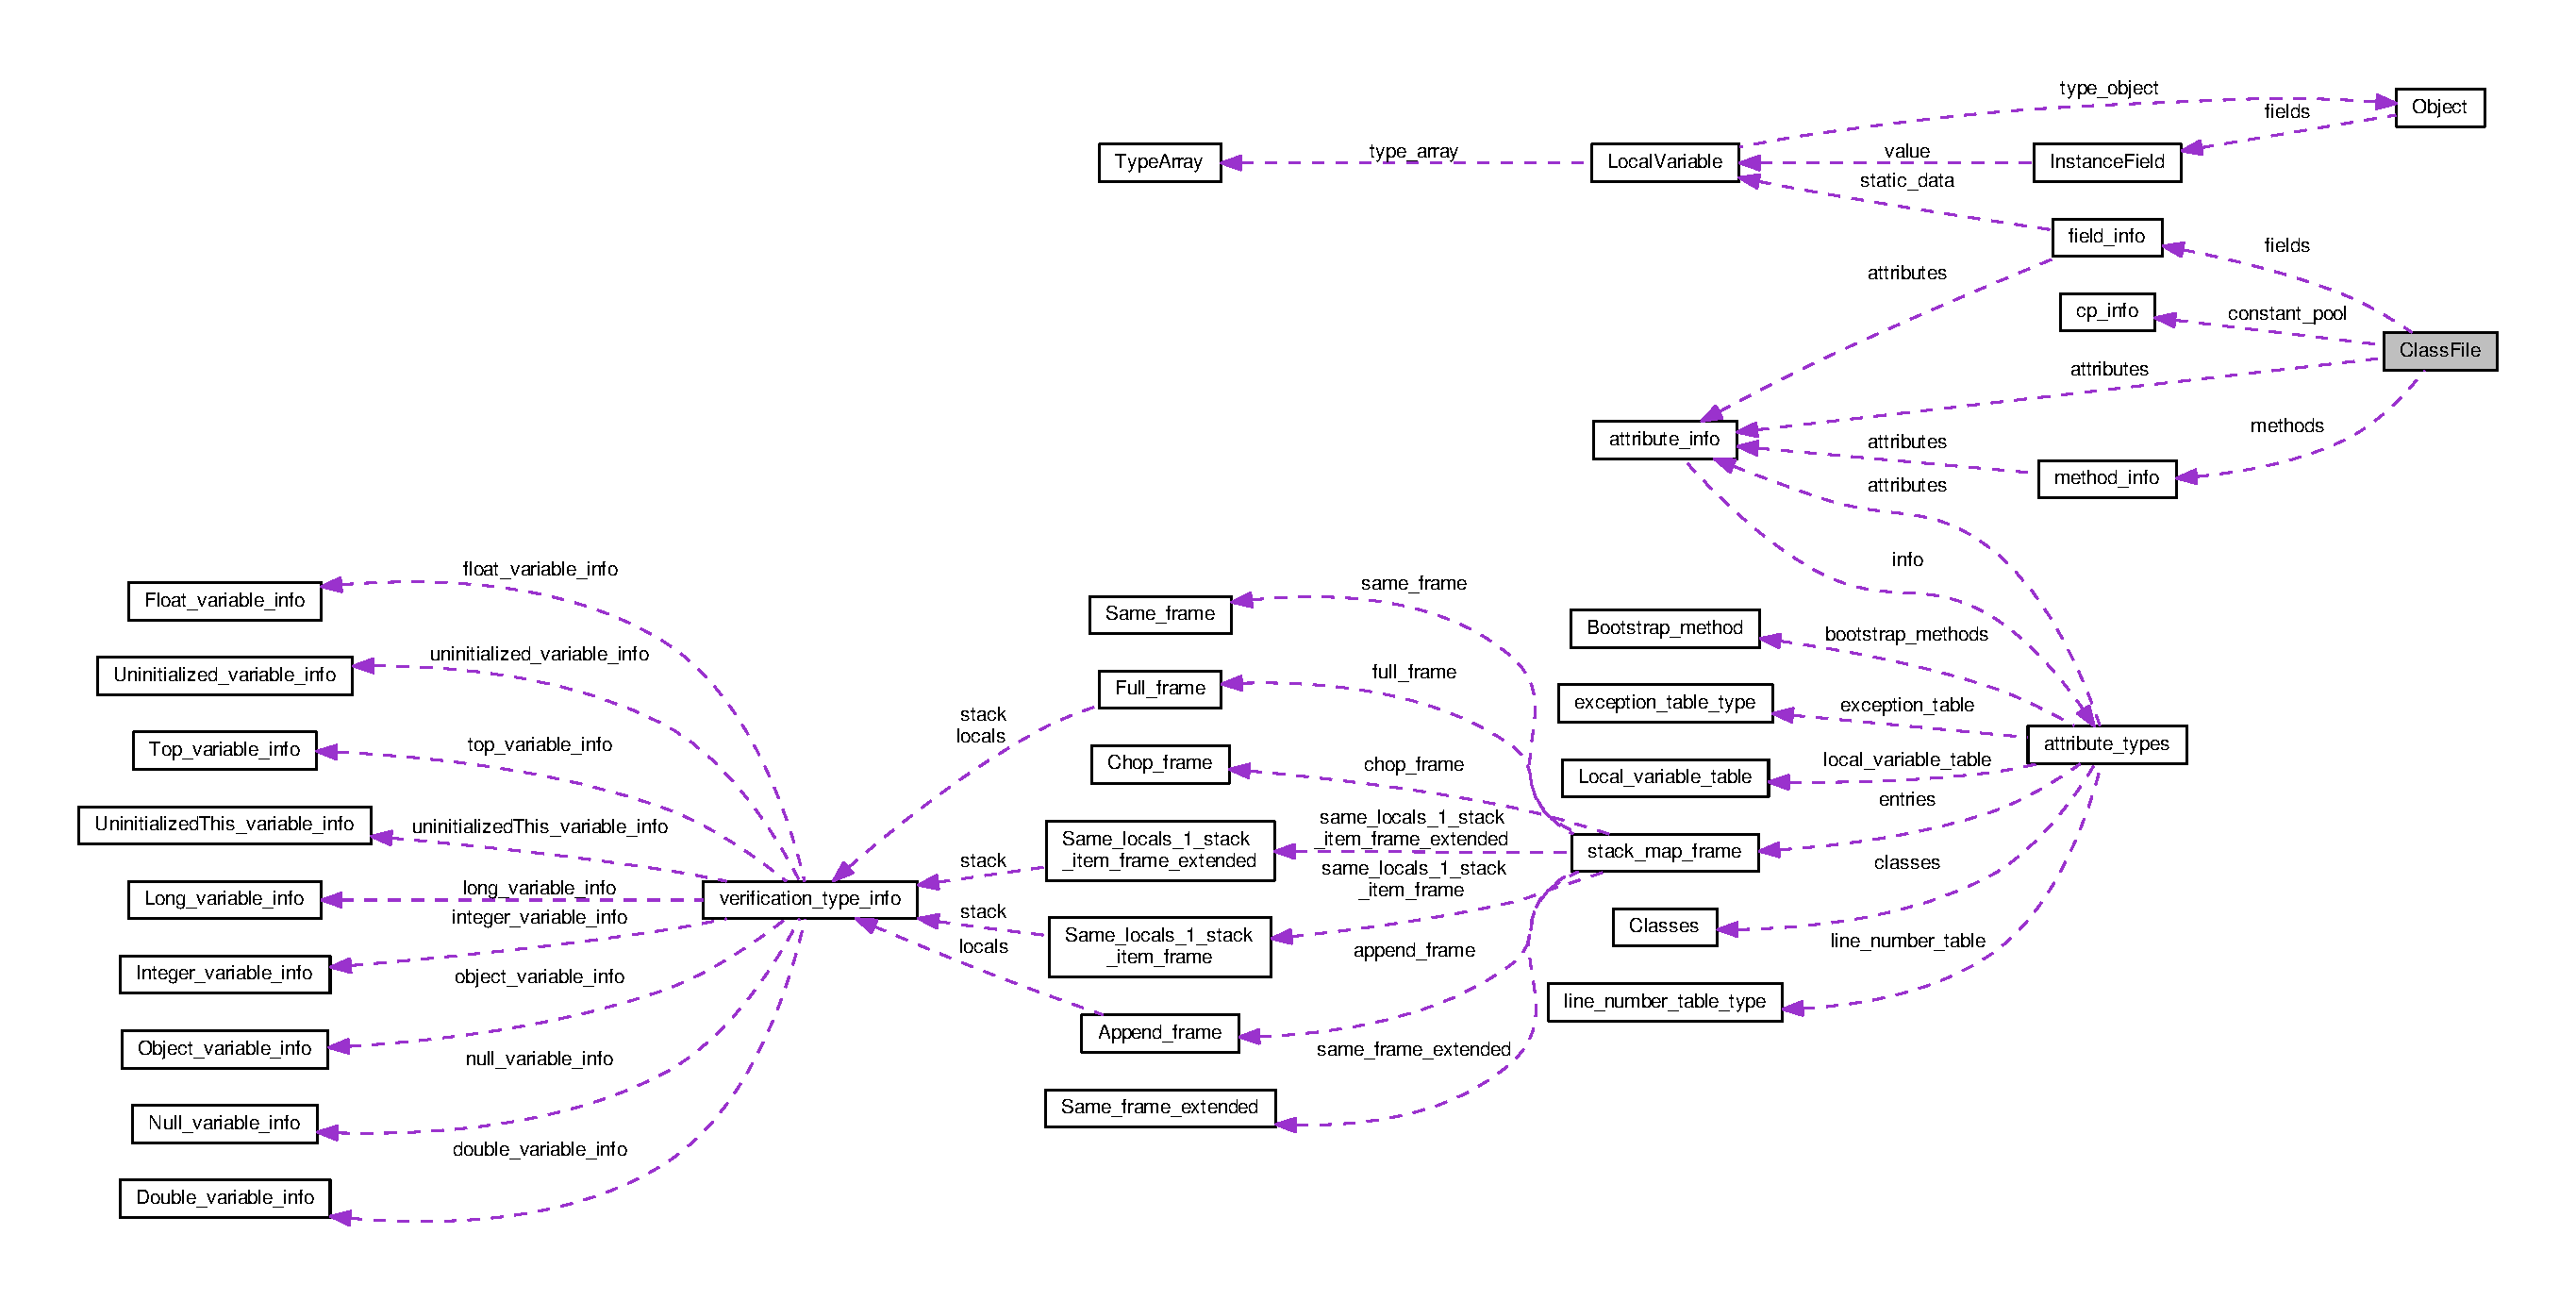
\includegraphics[width=350pt]{structClassFile__coll__graph}
\end{center}
\end{figure}
\subsection*{Public Attributes}
\begin{DoxyCompactItemize}
\item 
\hyperlink{structures_8h_ae391a1d79bb0c8cbc283f0283e3c098b}{u4} \hyperlink{structClassFile_a09085e9db513dae2f46da6e0a26c1b59}{magic}
\item 
\hyperlink{structures_8h_a55ef8d87fd202b8417704c089899c5b9}{u2} \hyperlink{structClassFile_af0db7b0ea01cb9cea2cee177ca81df09}{minor\+\_\+version}
\item 
\hyperlink{structures_8h_a55ef8d87fd202b8417704c089899c5b9}{u2} \hyperlink{structClassFile_abede9cb937e65072517d0ee6e26e2757}{major\+\_\+version}
\item 
\hyperlink{structures_8h_a55ef8d87fd202b8417704c089899c5b9}{u2} \hyperlink{structClassFile_ac8fdf5cccfd632da4fdb21ae63fffa7a}{constant\+\_\+pool\+\_\+count}
\item 
\hyperlink{structcp__info}{cp\+\_\+info} $\ast$ \hyperlink{structClassFile_a2309d843091aad79aed04ce92470a434}{constant\+\_\+pool}
\item 
\hyperlink{structures_8h_a55ef8d87fd202b8417704c089899c5b9}{u2} \hyperlink{structClassFile_ae88db578147f7ee0d6fc1aeacb341854}{access\+\_\+flags}
\item 
\hyperlink{structures_8h_a55ef8d87fd202b8417704c089899c5b9}{u2} \hyperlink{structClassFile_a2d33db0a560a71b94bc572dd1e4ec03a}{this\+\_\+class}
\item 
\hyperlink{structures_8h_a55ef8d87fd202b8417704c089899c5b9}{u2} \hyperlink{structClassFile_a5f6c11c0ccb02fd992b5c102725253ec}{super\+\_\+class}
\item 
\hyperlink{structures_8h_a55ef8d87fd202b8417704c089899c5b9}{u2} \hyperlink{structClassFile_a337fcb7da33d1b64631441115c7de305}{interfaces\+\_\+count}
\item 
\hyperlink{structures_8h_a55ef8d87fd202b8417704c089899c5b9}{u2} $\ast$ \hyperlink{structClassFile_af599de97e062c98966470f1590496425}{interfaces}
\item 
\hyperlink{structures_8h_a55ef8d87fd202b8417704c089899c5b9}{u2} \hyperlink{structClassFile_acea207ee523fbc16611d3cf436c390e0}{fields\+\_\+count}
\item 
\hyperlink{structfield__info}{field\+\_\+info} $\ast$ \hyperlink{structClassFile_aa324f88c75aa96c632f8c57d010aab0c}{fields}
\item 
\hyperlink{structures_8h_a55ef8d87fd202b8417704c089899c5b9}{u2} \hyperlink{structClassFile_aacfb45d4af64216324b1ae5269c870d5}{methods\+\_\+count}
\item 
\hyperlink{structmethod__info}{method\+\_\+info} $\ast$ \hyperlink{structClassFile_ad061f06cd709d10dbfbf82f443e43632}{methods}
\item 
\hyperlink{structures_8h_a55ef8d87fd202b8417704c089899c5b9}{u2} \hyperlink{structClassFile_a633c696fbe08e7e7906b2ab1e52f3d1b}{attributes\+\_\+count}
\item 
\hyperlink{structattribute__info}{attribute\+\_\+info} $\ast$ \hyperlink{structClassFile_a8bf809db8e1008f401dc3cda5e9cdb14}{attributes}
\end{DoxyCompactItemize}


\subsection{Detailed Description}
Struct que representa os campos do bytecode. 

Struct que representa o \hyperlink{structClassFile}{Class\+File}, para ser alocada pelo Class\+Loader e preenchida pela função \hyperlink{classfile_8c_a14c4d3f84dd03a43aca0a57bd530f3a2}{read\+\_\+class\+\_\+file()} 

\subsection{Member Data Documentation}
\index{Class\+File@{Class\+File}!access\+\_\+flags@{access\+\_\+flags}}
\index{access\+\_\+flags@{access\+\_\+flags}!Class\+File@{Class\+File}}
\subsubsection[{\texorpdfstring{access\+\_\+flags}{access_flags}}]{\setlength{\rightskip}{0pt plus 5cm}{\bf u2} Class\+File\+::access\+\_\+flags}\hypertarget{structClassFile_ae88db578147f7ee0d6fc1aeacb341854}{}\label{structClassFile_ae88db578147f7ee0d6fc1aeacb341854}
\index{Class\+File@{Class\+File}!attributes@{attributes}}
\index{attributes@{attributes}!Class\+File@{Class\+File}}
\subsubsection[{\texorpdfstring{attributes}{attributes}}]{\setlength{\rightskip}{0pt plus 5cm}{\bf attribute\+\_\+info}$\ast$ Class\+File\+::attributes}\hypertarget{structClassFile_a8bf809db8e1008f401dc3cda5e9cdb14}{}\label{structClassFile_a8bf809db8e1008f401dc3cda5e9cdb14}
\index{Class\+File@{Class\+File}!attributes\+\_\+count@{attributes\+\_\+count}}
\index{attributes\+\_\+count@{attributes\+\_\+count}!Class\+File@{Class\+File}}
\subsubsection[{\texorpdfstring{attributes\+\_\+count}{attributes_count}}]{\setlength{\rightskip}{0pt plus 5cm}{\bf u2} Class\+File\+::attributes\+\_\+count}\hypertarget{structClassFile_a633c696fbe08e7e7906b2ab1e52f3d1b}{}\label{structClassFile_a633c696fbe08e7e7906b2ab1e52f3d1b}
\index{Class\+File@{Class\+File}!constant\+\_\+pool@{constant\+\_\+pool}}
\index{constant\+\_\+pool@{constant\+\_\+pool}!Class\+File@{Class\+File}}
\subsubsection[{\texorpdfstring{constant\+\_\+pool}{constant_pool}}]{\setlength{\rightskip}{0pt plus 5cm}{\bf cp\+\_\+info}$\ast$ Class\+File\+::constant\+\_\+pool}\hypertarget{structClassFile_a2309d843091aad79aed04ce92470a434}{}\label{structClassFile_a2309d843091aad79aed04ce92470a434}
\index{Class\+File@{Class\+File}!constant\+\_\+pool\+\_\+count@{constant\+\_\+pool\+\_\+count}}
\index{constant\+\_\+pool\+\_\+count@{constant\+\_\+pool\+\_\+count}!Class\+File@{Class\+File}}
\subsubsection[{\texorpdfstring{constant\+\_\+pool\+\_\+count}{constant_pool_count}}]{\setlength{\rightskip}{0pt plus 5cm}{\bf u2} Class\+File\+::constant\+\_\+pool\+\_\+count}\hypertarget{structClassFile_ac8fdf5cccfd632da4fdb21ae63fffa7a}{}\label{structClassFile_ac8fdf5cccfd632da4fdb21ae63fffa7a}
\index{Class\+File@{Class\+File}!fields@{fields}}
\index{fields@{fields}!Class\+File@{Class\+File}}
\subsubsection[{\texorpdfstring{fields}{fields}}]{\setlength{\rightskip}{0pt plus 5cm}{\bf field\+\_\+info}$\ast$ Class\+File\+::fields}\hypertarget{structClassFile_aa324f88c75aa96c632f8c57d010aab0c}{}\label{structClassFile_aa324f88c75aa96c632f8c57d010aab0c}
\index{Class\+File@{Class\+File}!fields\+\_\+count@{fields\+\_\+count}}
\index{fields\+\_\+count@{fields\+\_\+count}!Class\+File@{Class\+File}}
\subsubsection[{\texorpdfstring{fields\+\_\+count}{fields_count}}]{\setlength{\rightskip}{0pt plus 5cm}{\bf u2} Class\+File\+::fields\+\_\+count}\hypertarget{structClassFile_acea207ee523fbc16611d3cf436c390e0}{}\label{structClassFile_acea207ee523fbc16611d3cf436c390e0}
\index{Class\+File@{Class\+File}!interfaces@{interfaces}}
\index{interfaces@{interfaces}!Class\+File@{Class\+File}}
\subsubsection[{\texorpdfstring{interfaces}{interfaces}}]{\setlength{\rightskip}{0pt plus 5cm}{\bf u2}$\ast$ Class\+File\+::interfaces}\hypertarget{structClassFile_af599de97e062c98966470f1590496425}{}\label{structClassFile_af599de97e062c98966470f1590496425}
\index{Class\+File@{Class\+File}!interfaces\+\_\+count@{interfaces\+\_\+count}}
\index{interfaces\+\_\+count@{interfaces\+\_\+count}!Class\+File@{Class\+File}}
\subsubsection[{\texorpdfstring{interfaces\+\_\+count}{interfaces_count}}]{\setlength{\rightskip}{0pt plus 5cm}{\bf u2} Class\+File\+::interfaces\+\_\+count}\hypertarget{structClassFile_a337fcb7da33d1b64631441115c7de305}{}\label{structClassFile_a337fcb7da33d1b64631441115c7de305}
\index{Class\+File@{Class\+File}!magic@{magic}}
\index{magic@{magic}!Class\+File@{Class\+File}}
\subsubsection[{\texorpdfstring{magic}{magic}}]{\setlength{\rightskip}{0pt plus 5cm}{\bf u4} Class\+File\+::magic}\hypertarget{structClassFile_a09085e9db513dae2f46da6e0a26c1b59}{}\label{structClassFile_a09085e9db513dae2f46da6e0a26c1b59}
\index{Class\+File@{Class\+File}!major\+\_\+version@{major\+\_\+version}}
\index{major\+\_\+version@{major\+\_\+version}!Class\+File@{Class\+File}}
\subsubsection[{\texorpdfstring{major\+\_\+version}{major_version}}]{\setlength{\rightskip}{0pt plus 5cm}{\bf u2} Class\+File\+::major\+\_\+version}\hypertarget{structClassFile_abede9cb937e65072517d0ee6e26e2757}{}\label{structClassFile_abede9cb937e65072517d0ee6e26e2757}
\index{Class\+File@{Class\+File}!methods@{methods}}
\index{methods@{methods}!Class\+File@{Class\+File}}
\subsubsection[{\texorpdfstring{methods}{methods}}]{\setlength{\rightskip}{0pt plus 5cm}{\bf method\+\_\+info}$\ast$ Class\+File\+::methods}\hypertarget{structClassFile_ad061f06cd709d10dbfbf82f443e43632}{}\label{structClassFile_ad061f06cd709d10dbfbf82f443e43632}
\index{Class\+File@{Class\+File}!methods\+\_\+count@{methods\+\_\+count}}
\index{methods\+\_\+count@{methods\+\_\+count}!Class\+File@{Class\+File}}
\subsubsection[{\texorpdfstring{methods\+\_\+count}{methods_count}}]{\setlength{\rightskip}{0pt plus 5cm}{\bf u2} Class\+File\+::methods\+\_\+count}\hypertarget{structClassFile_aacfb45d4af64216324b1ae5269c870d5}{}\label{structClassFile_aacfb45d4af64216324b1ae5269c870d5}
\index{Class\+File@{Class\+File}!minor\+\_\+version@{minor\+\_\+version}}
\index{minor\+\_\+version@{minor\+\_\+version}!Class\+File@{Class\+File}}
\subsubsection[{\texorpdfstring{minor\+\_\+version}{minor_version}}]{\setlength{\rightskip}{0pt plus 5cm}{\bf u2} Class\+File\+::minor\+\_\+version}\hypertarget{structClassFile_af0db7b0ea01cb9cea2cee177ca81df09}{}\label{structClassFile_af0db7b0ea01cb9cea2cee177ca81df09}
\index{Class\+File@{Class\+File}!super\+\_\+class@{super\+\_\+class}}
\index{super\+\_\+class@{super\+\_\+class}!Class\+File@{Class\+File}}
\subsubsection[{\texorpdfstring{super\+\_\+class}{super_class}}]{\setlength{\rightskip}{0pt plus 5cm}{\bf u2} Class\+File\+::super\+\_\+class}\hypertarget{structClassFile_a5f6c11c0ccb02fd992b5c102725253ec}{}\label{structClassFile_a5f6c11c0ccb02fd992b5c102725253ec}
\index{Class\+File@{Class\+File}!this\+\_\+class@{this\+\_\+class}}
\index{this\+\_\+class@{this\+\_\+class}!Class\+File@{Class\+File}}
\subsubsection[{\texorpdfstring{this\+\_\+class}{this_class}}]{\setlength{\rightskip}{0pt plus 5cm}{\bf u2} Class\+File\+::this\+\_\+class}\hypertarget{structClassFile_a2d33db0a560a71b94bc572dd1e4ec03a}{}\label{structClassFile_a2d33db0a560a71b94bc572dd1e4ec03a}


The documentation for this struct was generated from the following file\+:\begin{DoxyCompactItemize}
\item 
\hyperlink{structures_8h}{structures.\+h}\end{DoxyCompactItemize}

\hypertarget{structcp__info}{}\section{cp\+\_\+info Struct Reference}
\label{structcp__info}\index{cp\+\_\+info@{cp\+\_\+info}}


{\ttfamily \#include $<$structures.\+h$>$}

\subsection*{Public Attributes}
\begin{DoxyCompactItemize}
\item 
\hyperlink{structures_8h_a64f8055b64cf2a4c299c841130c5c938}{u1} \hyperlink{structcp__info_a045b8801a6e96a2a31d3b62ea684f141}{tag}
\item 
\begin{tabbing}
xx\=xx\=xx\=xx\=xx\=xx\=xx\=xx\=xx\=\kill
union \{\\
\>struct \{\\
\>\>\hyperlink{structures_8h_a55ef8d87fd202b8417704c089899c5b9}{u2} \hyperlink{structcp__info_a0b2c4677d0d56defd858fdc796caec87}{name\_index}\\
\>\} \hyperlink{structcp__info_a322117cc9b35710232212d96443b9c46}{Class}\\
\>struct \{\\
\>\>\hyperlink{structures_8h_a55ef8d87fd202b8417704c089899c5b9}{u2} \hyperlink{structcp__info_a1c7c3f3e2f9a620669b5f5cc51249ef8}{class\_index}\\
\>\>\hyperlink{structures_8h_a55ef8d87fd202b8417704c089899c5b9}{u2} \hyperlink{structcp__info_a1b947f3ff3eee58acf5500debf45848c}{name\_and\_type\_index}\\
\>\} \hyperlink{structcp__info_aee4742a1bbb698a449a95a88dfc6b4f9}{Fieldref}\\
\>struct \{\\
\>\>\hyperlink{structures_8h_a55ef8d87fd202b8417704c089899c5b9}{u2} \hyperlink{structcp__info_a1c7c3f3e2f9a620669b5f5cc51249ef8}{class\_index}\\
\>\>\hyperlink{structures_8h_a55ef8d87fd202b8417704c089899c5b9}{u2} \hyperlink{structcp__info_a1b947f3ff3eee58acf5500debf45848c}{name\_and\_type\_index}\\
\>\} \hyperlink{structcp__info_ae02638b6c90e9d24eae9c8bfc4b09f1c}{Methodref}\\
\>struct \{\\
\>\>\hyperlink{structures_8h_a55ef8d87fd202b8417704c089899c5b9}{u2} \hyperlink{structcp__info_a1c7c3f3e2f9a620669b5f5cc51249ef8}{class\_index}\\
\>\>\hyperlink{structures_8h_a55ef8d87fd202b8417704c089899c5b9}{u2} \hyperlink{structcp__info_a1b947f3ff3eee58acf5500debf45848c}{name\_and\_type\_index}\\
\>\} \hyperlink{structcp__info_a4bc2525cea570eff1133480f351ab833}{InterfaceMethodref}\\
\>struct \{\\
\>\>\hyperlink{structures_8h_a55ef8d87fd202b8417704c089899c5b9}{u2} \hyperlink{structcp__info_ae760e12a2ee01b0ace3d35170ca07981}{string\_index}\\
\>\} \hyperlink{structcp__info_a453cf965166c542ff75a14db651769e3}{String}\\
\>struct \{\\
\>\>\hyperlink{structures_8h_ae391a1d79bb0c8cbc283f0283e3c098b}{u4} \hyperlink{structcp__info_a4dcce18f4a19e8112079dc11dc2f5386}{bytes}\\
\>\} \hyperlink{structcp__info_ada2bb1a48d398e9ecaf3180eb82bbd32}{Integer}\\
\>struct \{\\
\>\>\hyperlink{structures_8h_ae391a1d79bb0c8cbc283f0283e3c098b}{u4} \hyperlink{structcp__info_a4dcce18f4a19e8112079dc11dc2f5386}{bytes}\\
\>\} \hyperlink{structcp__info_ae1a57be30f86f89552e556c01a186461}{Float}\\
\>struct \{\\
\>\>\hyperlink{structures_8h_ae391a1d79bb0c8cbc283f0283e3c098b}{u4} \hyperlink{structcp__info_a26996f9b4a0caab37c9cdbfd027eaed7}{high\_bytes}\\
\>\>\hyperlink{structures_8h_ae391a1d79bb0c8cbc283f0283e3c098b}{u4} \hyperlink{structcp__info_aff872b9dcff18e083ca9f73ef82ab14f}{low\_bytes}\\
\>\} \hyperlink{structcp__info_aaef6412a3f5c1011817df7889b13461d}{Long}\\
\>struct \{\\
\>\>\hyperlink{structures_8h_ae391a1d79bb0c8cbc283f0283e3c098b}{u4} \hyperlink{structcp__info_a26996f9b4a0caab37c9cdbfd027eaed7}{high\_bytes}\\
\>\>\hyperlink{structures_8h_ae391a1d79bb0c8cbc283f0283e3c098b}{u4} \hyperlink{structcp__info_aff872b9dcff18e083ca9f73ef82ab14f}{low\_bytes}\\
\>\} \hyperlink{structcp__info_ac501a57eed33b25313614096d0b2d80c}{Double}\\
\>struct \{\\
\>\>\hyperlink{structures_8h_a55ef8d87fd202b8417704c089899c5b9}{u2} \hyperlink{structcp__info_a0b2c4677d0d56defd858fdc796caec87}{name\_index}\\
\>\>\hyperlink{structures_8h_a55ef8d87fd202b8417704c089899c5b9}{u2} \hyperlink{structcp__info_a35ec31f117bf83ef9aef6100822f1141}{descriptor\_index}\\
\>\} \hyperlink{structcp__info_ac43e804549f01bed269b46ac2fd0efca}{NameAndType}\\
\>struct \{\\
\>\>\hyperlink{structures_8h_a55ef8d87fd202b8417704c089899c5b9}{u2} \hyperlink{structcp__info_a1df458be110c843ea49b8a8a4c9dfb91}{length}\\
\>\>\hyperlink{structures_8h_a64f8055b64cf2a4c299c841130c5c938}{u1} $\ast$ \hyperlink{structcp__info_a30f97eda54e30a923a217520316e9301}{bytes}\\
\>\} \hyperlink{structcp__info_af0b0a05e0079e3d1b0c99cd3c0e4463a}{Utf8}\\
\>struct \{\\
\>\>\hyperlink{structures_8h_a64f8055b64cf2a4c299c841130c5c938}{u1} \hyperlink{structcp__info_a13e5aa07b7aa482061b89f4d7379a2dd}{reference\_kind}\\
\>\>\hyperlink{structures_8h_a55ef8d87fd202b8417704c089899c5b9}{u2} \hyperlink{structcp__info_a946bbab9aa280d4e22194ef7b434166a}{reference\_index}\\
\>\} \hyperlink{structcp__info_a6a4f93d961e65bc33c079ba656b89884}{MethodHandle}\\
\>struct \{\\
\>\>\hyperlink{structures_8h_a55ef8d87fd202b8417704c089899c5b9}{u2} \hyperlink{structcp__info_a35ec31f117bf83ef9aef6100822f1141}{descriptor\_index}\\
\>\} \hyperlink{structcp__info_a2faf7cea4242acbc5f952567fdabfb72}{MethodType}\\
\>struct \{\\
\>\>\hyperlink{structures_8h_a55ef8d87fd202b8417704c089899c5b9}{u2} \hyperlink{structcp__info_abad11f89efc244065e72ec811f9dc929}{bootstrap\_method\_attr\_index}\\
\>\>\hyperlink{structures_8h_a55ef8d87fd202b8417704c089899c5b9}{u2} \hyperlink{structcp__info_a1b947f3ff3eee58acf5500debf45848c}{name\_and\_type\_index}\\
\>\} \hyperlink{structcp__info_a9f368f50ec505be7deadf4af55074cdd}{InvokeDynamic}\\
\}; \\

\end{tabbing}\end{DoxyCompactItemize}


\subsection{Detailed Description}
Struct para indicar o tipo de constant\+\_\+pool (tendo uma tag associada e mais atributos em função da constante)

Union\+: serve para alocar espaço pra maior struct 

\subsection{Member Data Documentation}
\subsubsection[{\texorpdfstring{"@5}{@5}}]{\setlength{\rightskip}{0pt plus 5cm}union \{ ... \} }\hypertarget{structcp__info_a0469358e891d5c89038d59f1807d00b2}{}\label{structcp__info_a0469358e891d5c89038d59f1807d00b2}
\index{cp\+\_\+info@{cp\+\_\+info}!bootstrap\+\_\+method\+\_\+attr\+\_\+index@{bootstrap\+\_\+method\+\_\+attr\+\_\+index}}
\index{bootstrap\+\_\+method\+\_\+attr\+\_\+index@{bootstrap\+\_\+method\+\_\+attr\+\_\+index}!cp\+\_\+info@{cp\+\_\+info}}
\subsubsection[{\texorpdfstring{bootstrap\+\_\+method\+\_\+attr\+\_\+index}{bootstrap_method_attr_index}}]{\setlength{\rightskip}{0pt plus 5cm}{\bf u2} cp\+\_\+info\+::bootstrap\+\_\+method\+\_\+attr\+\_\+index}\hypertarget{structcp__info_abad11f89efc244065e72ec811f9dc929}{}\label{structcp__info_abad11f89efc244065e72ec811f9dc929}
\index{cp\+\_\+info@{cp\+\_\+info}!bytes@{bytes}}
\index{bytes@{bytes}!cp\+\_\+info@{cp\+\_\+info}}
\subsubsection[{\texorpdfstring{bytes}{bytes}}]{\setlength{\rightskip}{0pt plus 5cm}{\bf u4} cp\+\_\+info\+::bytes}\hypertarget{structcp__info_a4dcce18f4a19e8112079dc11dc2f5386}{}\label{structcp__info_a4dcce18f4a19e8112079dc11dc2f5386}
\index{cp\+\_\+info@{cp\+\_\+info}!bytes@{bytes}}
\index{bytes@{bytes}!cp\+\_\+info@{cp\+\_\+info}}
\subsubsection[{\texorpdfstring{bytes}{bytes}}]{\setlength{\rightskip}{0pt plus 5cm}{\bf u1}$\ast$ cp\+\_\+info\+::bytes}\hypertarget{structcp__info_a30f97eda54e30a923a217520316e9301}{}\label{structcp__info_a30f97eda54e30a923a217520316e9301}
\index{cp\+\_\+info@{cp\+\_\+info}!Class@{Class}}
\index{Class@{Class}!cp\+\_\+info@{cp\+\_\+info}}
\subsubsection[{\texorpdfstring{Class}{Class}}]{\setlength{\rightskip}{0pt plus 5cm}struct \{ ... \}   cp\+\_\+info\+::\+Class}\hypertarget{structcp__info_a322117cc9b35710232212d96443b9c46}{}\label{structcp__info_a322117cc9b35710232212d96443b9c46}
\index{cp\+\_\+info@{cp\+\_\+info}!class\+\_\+index@{class\+\_\+index}}
\index{class\+\_\+index@{class\+\_\+index}!cp\+\_\+info@{cp\+\_\+info}}
\subsubsection[{\texorpdfstring{class\+\_\+index}{class_index}}]{\setlength{\rightskip}{0pt plus 5cm}{\bf u2} cp\+\_\+info\+::class\+\_\+index}\hypertarget{structcp__info_a1c7c3f3e2f9a620669b5f5cc51249ef8}{}\label{structcp__info_a1c7c3f3e2f9a620669b5f5cc51249ef8}
\index{cp\+\_\+info@{cp\+\_\+info}!descriptor\+\_\+index@{descriptor\+\_\+index}}
\index{descriptor\+\_\+index@{descriptor\+\_\+index}!cp\+\_\+info@{cp\+\_\+info}}
\subsubsection[{\texorpdfstring{descriptor\+\_\+index}{descriptor_index}}]{\setlength{\rightskip}{0pt plus 5cm}{\bf u2} cp\+\_\+info\+::descriptor\+\_\+index}\hypertarget{structcp__info_a35ec31f117bf83ef9aef6100822f1141}{}\label{structcp__info_a35ec31f117bf83ef9aef6100822f1141}
\index{cp\+\_\+info@{cp\+\_\+info}!Double@{Double}}
\index{Double@{Double}!cp\+\_\+info@{cp\+\_\+info}}
\subsubsection[{\texorpdfstring{Double}{Double}}]{\setlength{\rightskip}{0pt plus 5cm}struct \{ ... \}   cp\+\_\+info\+::\+Double}\hypertarget{structcp__info_ac501a57eed33b25313614096d0b2d80c}{}\label{structcp__info_ac501a57eed33b25313614096d0b2d80c}
\index{cp\+\_\+info@{cp\+\_\+info}!Fieldref@{Fieldref}}
\index{Fieldref@{Fieldref}!cp\+\_\+info@{cp\+\_\+info}}
\subsubsection[{\texorpdfstring{Fieldref}{Fieldref}}]{\setlength{\rightskip}{0pt plus 5cm}struct \{ ... \}   cp\+\_\+info\+::\+Fieldref}\hypertarget{structcp__info_aee4742a1bbb698a449a95a88dfc6b4f9}{}\label{structcp__info_aee4742a1bbb698a449a95a88dfc6b4f9}
\index{cp\+\_\+info@{cp\+\_\+info}!Float@{Float}}
\index{Float@{Float}!cp\+\_\+info@{cp\+\_\+info}}
\subsubsection[{\texorpdfstring{Float}{Float}}]{\setlength{\rightskip}{0pt plus 5cm}struct \{ ... \}   cp\+\_\+info\+::\+Float}\hypertarget{structcp__info_ae1a57be30f86f89552e556c01a186461}{}\label{structcp__info_ae1a57be30f86f89552e556c01a186461}
\index{cp\+\_\+info@{cp\+\_\+info}!high\+\_\+bytes@{high\+\_\+bytes}}
\index{high\+\_\+bytes@{high\+\_\+bytes}!cp\+\_\+info@{cp\+\_\+info}}
\subsubsection[{\texorpdfstring{high\+\_\+bytes}{high_bytes}}]{\setlength{\rightskip}{0pt plus 5cm}{\bf u4} cp\+\_\+info\+::high\+\_\+bytes}\hypertarget{structcp__info_a26996f9b4a0caab37c9cdbfd027eaed7}{}\label{structcp__info_a26996f9b4a0caab37c9cdbfd027eaed7}
\index{cp\+\_\+info@{cp\+\_\+info}!Integer@{Integer}}
\index{Integer@{Integer}!cp\+\_\+info@{cp\+\_\+info}}
\subsubsection[{\texorpdfstring{Integer}{Integer}}]{\setlength{\rightskip}{0pt plus 5cm}struct \{ ... \}   cp\+\_\+info\+::\+Integer}\hypertarget{structcp__info_ada2bb1a48d398e9ecaf3180eb82bbd32}{}\label{structcp__info_ada2bb1a48d398e9ecaf3180eb82bbd32}
\index{cp\+\_\+info@{cp\+\_\+info}!Interface\+Methodref@{Interface\+Methodref}}
\index{Interface\+Methodref@{Interface\+Methodref}!cp\+\_\+info@{cp\+\_\+info}}
\subsubsection[{\texorpdfstring{Interface\+Methodref}{InterfaceMethodref}}]{\setlength{\rightskip}{0pt plus 5cm}struct \{ ... \}   cp\+\_\+info\+::\+Interface\+Methodref}\hypertarget{structcp__info_a4bc2525cea570eff1133480f351ab833}{}\label{structcp__info_a4bc2525cea570eff1133480f351ab833}
\index{cp\+\_\+info@{cp\+\_\+info}!Invoke\+Dynamic@{Invoke\+Dynamic}}
\index{Invoke\+Dynamic@{Invoke\+Dynamic}!cp\+\_\+info@{cp\+\_\+info}}
\subsubsection[{\texorpdfstring{Invoke\+Dynamic}{InvokeDynamic}}]{\setlength{\rightskip}{0pt plus 5cm}struct \{ ... \}   cp\+\_\+info\+::\+Invoke\+Dynamic}\hypertarget{structcp__info_a9f368f50ec505be7deadf4af55074cdd}{}\label{structcp__info_a9f368f50ec505be7deadf4af55074cdd}
\index{cp\+\_\+info@{cp\+\_\+info}!length@{length}}
\index{length@{length}!cp\+\_\+info@{cp\+\_\+info}}
\subsubsection[{\texorpdfstring{length}{length}}]{\setlength{\rightskip}{0pt plus 5cm}{\bf u2} cp\+\_\+info\+::length}\hypertarget{structcp__info_a1df458be110c843ea49b8a8a4c9dfb91}{}\label{structcp__info_a1df458be110c843ea49b8a8a4c9dfb91}
\index{cp\+\_\+info@{cp\+\_\+info}!Long@{Long}}
\index{Long@{Long}!cp\+\_\+info@{cp\+\_\+info}}
\subsubsection[{\texorpdfstring{Long}{Long}}]{\setlength{\rightskip}{0pt plus 5cm}struct \{ ... \}   cp\+\_\+info\+::\+Long}\hypertarget{structcp__info_aaef6412a3f5c1011817df7889b13461d}{}\label{structcp__info_aaef6412a3f5c1011817df7889b13461d}
\index{cp\+\_\+info@{cp\+\_\+info}!low\+\_\+bytes@{low\+\_\+bytes}}
\index{low\+\_\+bytes@{low\+\_\+bytes}!cp\+\_\+info@{cp\+\_\+info}}
\subsubsection[{\texorpdfstring{low\+\_\+bytes}{low_bytes}}]{\setlength{\rightskip}{0pt plus 5cm}{\bf u4} cp\+\_\+info\+::low\+\_\+bytes}\hypertarget{structcp__info_aff872b9dcff18e083ca9f73ef82ab14f}{}\label{structcp__info_aff872b9dcff18e083ca9f73ef82ab14f}
\index{cp\+\_\+info@{cp\+\_\+info}!Method\+Handle@{Method\+Handle}}
\index{Method\+Handle@{Method\+Handle}!cp\+\_\+info@{cp\+\_\+info}}
\subsubsection[{\texorpdfstring{Method\+Handle}{MethodHandle}}]{\setlength{\rightskip}{0pt plus 5cm}struct \{ ... \}   cp\+\_\+info\+::\+Method\+Handle}\hypertarget{structcp__info_a6a4f93d961e65bc33c079ba656b89884}{}\label{structcp__info_a6a4f93d961e65bc33c079ba656b89884}
\index{cp\+\_\+info@{cp\+\_\+info}!Methodref@{Methodref}}
\index{Methodref@{Methodref}!cp\+\_\+info@{cp\+\_\+info}}
\subsubsection[{\texorpdfstring{Methodref}{Methodref}}]{\setlength{\rightskip}{0pt plus 5cm}struct \{ ... \}   cp\+\_\+info\+::\+Methodref}\hypertarget{structcp__info_ae02638b6c90e9d24eae9c8bfc4b09f1c}{}\label{structcp__info_ae02638b6c90e9d24eae9c8bfc4b09f1c}
\index{cp\+\_\+info@{cp\+\_\+info}!Method\+Type@{Method\+Type}}
\index{Method\+Type@{Method\+Type}!cp\+\_\+info@{cp\+\_\+info}}
\subsubsection[{\texorpdfstring{Method\+Type}{MethodType}}]{\setlength{\rightskip}{0pt plus 5cm}struct \{ ... \}   cp\+\_\+info\+::\+Method\+Type}\hypertarget{structcp__info_a2faf7cea4242acbc5f952567fdabfb72}{}\label{structcp__info_a2faf7cea4242acbc5f952567fdabfb72}
\index{cp\+\_\+info@{cp\+\_\+info}!name\+\_\+and\+\_\+type\+\_\+index@{name\+\_\+and\+\_\+type\+\_\+index}}
\index{name\+\_\+and\+\_\+type\+\_\+index@{name\+\_\+and\+\_\+type\+\_\+index}!cp\+\_\+info@{cp\+\_\+info}}
\subsubsection[{\texorpdfstring{name\+\_\+and\+\_\+type\+\_\+index}{name_and_type_index}}]{\setlength{\rightskip}{0pt plus 5cm}{\bf u2} cp\+\_\+info\+::name\+\_\+and\+\_\+type\+\_\+index}\hypertarget{structcp__info_a1b947f3ff3eee58acf5500debf45848c}{}\label{structcp__info_a1b947f3ff3eee58acf5500debf45848c}
\index{cp\+\_\+info@{cp\+\_\+info}!name\+\_\+index@{name\+\_\+index}}
\index{name\+\_\+index@{name\+\_\+index}!cp\+\_\+info@{cp\+\_\+info}}
\subsubsection[{\texorpdfstring{name\+\_\+index}{name_index}}]{\setlength{\rightskip}{0pt plus 5cm}{\bf u2} cp\+\_\+info\+::name\+\_\+index}\hypertarget{structcp__info_a0b2c4677d0d56defd858fdc796caec87}{}\label{structcp__info_a0b2c4677d0d56defd858fdc796caec87}
\index{cp\+\_\+info@{cp\+\_\+info}!Name\+And\+Type@{Name\+And\+Type}}
\index{Name\+And\+Type@{Name\+And\+Type}!cp\+\_\+info@{cp\+\_\+info}}
\subsubsection[{\texorpdfstring{Name\+And\+Type}{NameAndType}}]{\setlength{\rightskip}{0pt plus 5cm}struct \{ ... \}   cp\+\_\+info\+::\+Name\+And\+Type}\hypertarget{structcp__info_ac43e804549f01bed269b46ac2fd0efca}{}\label{structcp__info_ac43e804549f01bed269b46ac2fd0efca}
\index{cp\+\_\+info@{cp\+\_\+info}!reference\+\_\+index@{reference\+\_\+index}}
\index{reference\+\_\+index@{reference\+\_\+index}!cp\+\_\+info@{cp\+\_\+info}}
\subsubsection[{\texorpdfstring{reference\+\_\+index}{reference_index}}]{\setlength{\rightskip}{0pt plus 5cm}{\bf u2} cp\+\_\+info\+::reference\+\_\+index}\hypertarget{structcp__info_a946bbab9aa280d4e22194ef7b434166a}{}\label{structcp__info_a946bbab9aa280d4e22194ef7b434166a}
\index{cp\+\_\+info@{cp\+\_\+info}!reference\+\_\+kind@{reference\+\_\+kind}}
\index{reference\+\_\+kind@{reference\+\_\+kind}!cp\+\_\+info@{cp\+\_\+info}}
\subsubsection[{\texorpdfstring{reference\+\_\+kind}{reference_kind}}]{\setlength{\rightskip}{0pt plus 5cm}{\bf u1} cp\+\_\+info\+::reference\+\_\+kind}\hypertarget{structcp__info_a13e5aa07b7aa482061b89f4d7379a2dd}{}\label{structcp__info_a13e5aa07b7aa482061b89f4d7379a2dd}
\index{cp\+\_\+info@{cp\+\_\+info}!String@{String}}
\index{String@{String}!cp\+\_\+info@{cp\+\_\+info}}
\subsubsection[{\texorpdfstring{String}{String}}]{\setlength{\rightskip}{0pt plus 5cm}struct \{ ... \}   cp\+\_\+info\+::\+String}\hypertarget{structcp__info_a453cf965166c542ff75a14db651769e3}{}\label{structcp__info_a453cf965166c542ff75a14db651769e3}
\index{cp\+\_\+info@{cp\+\_\+info}!string\+\_\+index@{string\+\_\+index}}
\index{string\+\_\+index@{string\+\_\+index}!cp\+\_\+info@{cp\+\_\+info}}
\subsubsection[{\texorpdfstring{string\+\_\+index}{string_index}}]{\setlength{\rightskip}{0pt plus 5cm}{\bf u2} cp\+\_\+info\+::string\+\_\+index}\hypertarget{structcp__info_ae760e12a2ee01b0ace3d35170ca07981}{}\label{structcp__info_ae760e12a2ee01b0ace3d35170ca07981}
\index{cp\+\_\+info@{cp\+\_\+info}!tag@{tag}}
\index{tag@{tag}!cp\+\_\+info@{cp\+\_\+info}}
\subsubsection[{\texorpdfstring{tag}{tag}}]{\setlength{\rightskip}{0pt plus 5cm}{\bf u1} cp\+\_\+info\+::tag}\hypertarget{structcp__info_a045b8801a6e96a2a31d3b62ea684f141}{}\label{structcp__info_a045b8801a6e96a2a31d3b62ea684f141}
\index{cp\+\_\+info@{cp\+\_\+info}!Utf8@{Utf8}}
\index{Utf8@{Utf8}!cp\+\_\+info@{cp\+\_\+info}}
\subsubsection[{\texorpdfstring{Utf8}{Utf8}}]{\setlength{\rightskip}{0pt plus 5cm}struct \{ ... \}   cp\+\_\+info\+::\+Utf8}\hypertarget{structcp__info_af0b0a05e0079e3d1b0c99cd3c0e4463a}{}\label{structcp__info_af0b0a05e0079e3d1b0c99cd3c0e4463a}


The documentation for this struct was generated from the following file\+:\begin{DoxyCompactItemize}
\item 
\hyperlink{structures_8h}{structures.\+h}\end{DoxyCompactItemize}

\hypertarget{structDouble__variable__info}{}\section{Double\+\_\+variable\+\_\+info Struct Reference}
\label{structDouble__variable__info}\index{Double\+\_\+variable\+\_\+info@{Double\+\_\+variable\+\_\+info}}


{\ttfamily \#include $<$structures.\+h$>$}



The documentation for this struct was generated from the following file\+:\begin{DoxyCompactItemize}
\item 
\hyperlink{structures_8h}{structures.\+h}\end{DoxyCompactItemize}

\hypertarget{structexception__table__type}{}\section{exception\+\_\+table\+\_\+type Struct Reference}
\label{structexception__table__type}\index{exception\+\_\+table\+\_\+type@{exception\+\_\+table\+\_\+type}}


{\ttfamily \#include $<$structures.\+h$>$}

\subsection*{Public Attributes}
\begin{DoxyCompactItemize}
\item 
\hyperlink{structures_8h_a55ef8d87fd202b8417704c089899c5b9}{u2} \hyperlink{structexception__table__type_a71cf8eaa3d06b89818100df6405b266d}{start\+\_\+pc}
\item 
\hyperlink{structures_8h_a55ef8d87fd202b8417704c089899c5b9}{u2} \hyperlink{structexception__table__type_a796565865a227dc76b0dd7c78e3f8424}{end\+\_\+pc}
\item 
\hyperlink{structures_8h_a55ef8d87fd202b8417704c089899c5b9}{u2} \hyperlink{structexception__table__type_af1b56d902850a41f63b7271029946759}{handler\+\_\+pc}
\item 
\hyperlink{structures_8h_a55ef8d87fd202b8417704c089899c5b9}{u2} \hyperlink{structexception__table__type_a663fa7b2d1a468b29913fd92e006a5dc}{catch\+\_\+type}
\end{DoxyCompactItemize}


\subsection{Member Data Documentation}
\index{exception\+\_\+table\+\_\+type@{exception\+\_\+table\+\_\+type}!catch\+\_\+type@{catch\+\_\+type}}
\index{catch\+\_\+type@{catch\+\_\+type}!exception\+\_\+table\+\_\+type@{exception\+\_\+table\+\_\+type}}
\subsubsection[{\texorpdfstring{catch\+\_\+type}{catch_type}}]{\setlength{\rightskip}{0pt plus 5cm}{\bf u2} exception\+\_\+table\+\_\+type\+::catch\+\_\+type}\hypertarget{structexception__table__type_a663fa7b2d1a468b29913fd92e006a5dc}{}\label{structexception__table__type_a663fa7b2d1a468b29913fd92e006a5dc}
\index{exception\+\_\+table\+\_\+type@{exception\+\_\+table\+\_\+type}!end\+\_\+pc@{end\+\_\+pc}}
\index{end\+\_\+pc@{end\+\_\+pc}!exception\+\_\+table\+\_\+type@{exception\+\_\+table\+\_\+type}}
\subsubsection[{\texorpdfstring{end\+\_\+pc}{end_pc}}]{\setlength{\rightskip}{0pt plus 5cm}{\bf u2} exception\+\_\+table\+\_\+type\+::end\+\_\+pc}\hypertarget{structexception__table__type_a796565865a227dc76b0dd7c78e3f8424}{}\label{structexception__table__type_a796565865a227dc76b0dd7c78e3f8424}
\index{exception\+\_\+table\+\_\+type@{exception\+\_\+table\+\_\+type}!handler\+\_\+pc@{handler\+\_\+pc}}
\index{handler\+\_\+pc@{handler\+\_\+pc}!exception\+\_\+table\+\_\+type@{exception\+\_\+table\+\_\+type}}
\subsubsection[{\texorpdfstring{handler\+\_\+pc}{handler_pc}}]{\setlength{\rightskip}{0pt plus 5cm}{\bf u2} exception\+\_\+table\+\_\+type\+::handler\+\_\+pc}\hypertarget{structexception__table__type_af1b56d902850a41f63b7271029946759}{}\label{structexception__table__type_af1b56d902850a41f63b7271029946759}
\index{exception\+\_\+table\+\_\+type@{exception\+\_\+table\+\_\+type}!start\+\_\+pc@{start\+\_\+pc}}
\index{start\+\_\+pc@{start\+\_\+pc}!exception\+\_\+table\+\_\+type@{exception\+\_\+table\+\_\+type}}
\subsubsection[{\texorpdfstring{start\+\_\+pc}{start_pc}}]{\setlength{\rightskip}{0pt plus 5cm}{\bf u2} exception\+\_\+table\+\_\+type\+::start\+\_\+pc}\hypertarget{structexception__table__type_a71cf8eaa3d06b89818100df6405b266d}{}\label{structexception__table__type_a71cf8eaa3d06b89818100df6405b266d}


The documentation for this struct was generated from the following file\+:\begin{DoxyCompactItemize}
\item 
\hyperlink{structures_8h}{structures.\+h}\end{DoxyCompactItemize}

\hypertarget{structfield__info}{}\section{field\+\_\+info Struct Reference}
\label{structfield__info}\index{field\+\_\+info@{field\+\_\+info}}


{\ttfamily \#include $<$structures.\+h$>$}



Collaboration diagram for field\+\_\+info\+:
\nopagebreak
\begin{figure}[H]
\begin{center}
\leavevmode
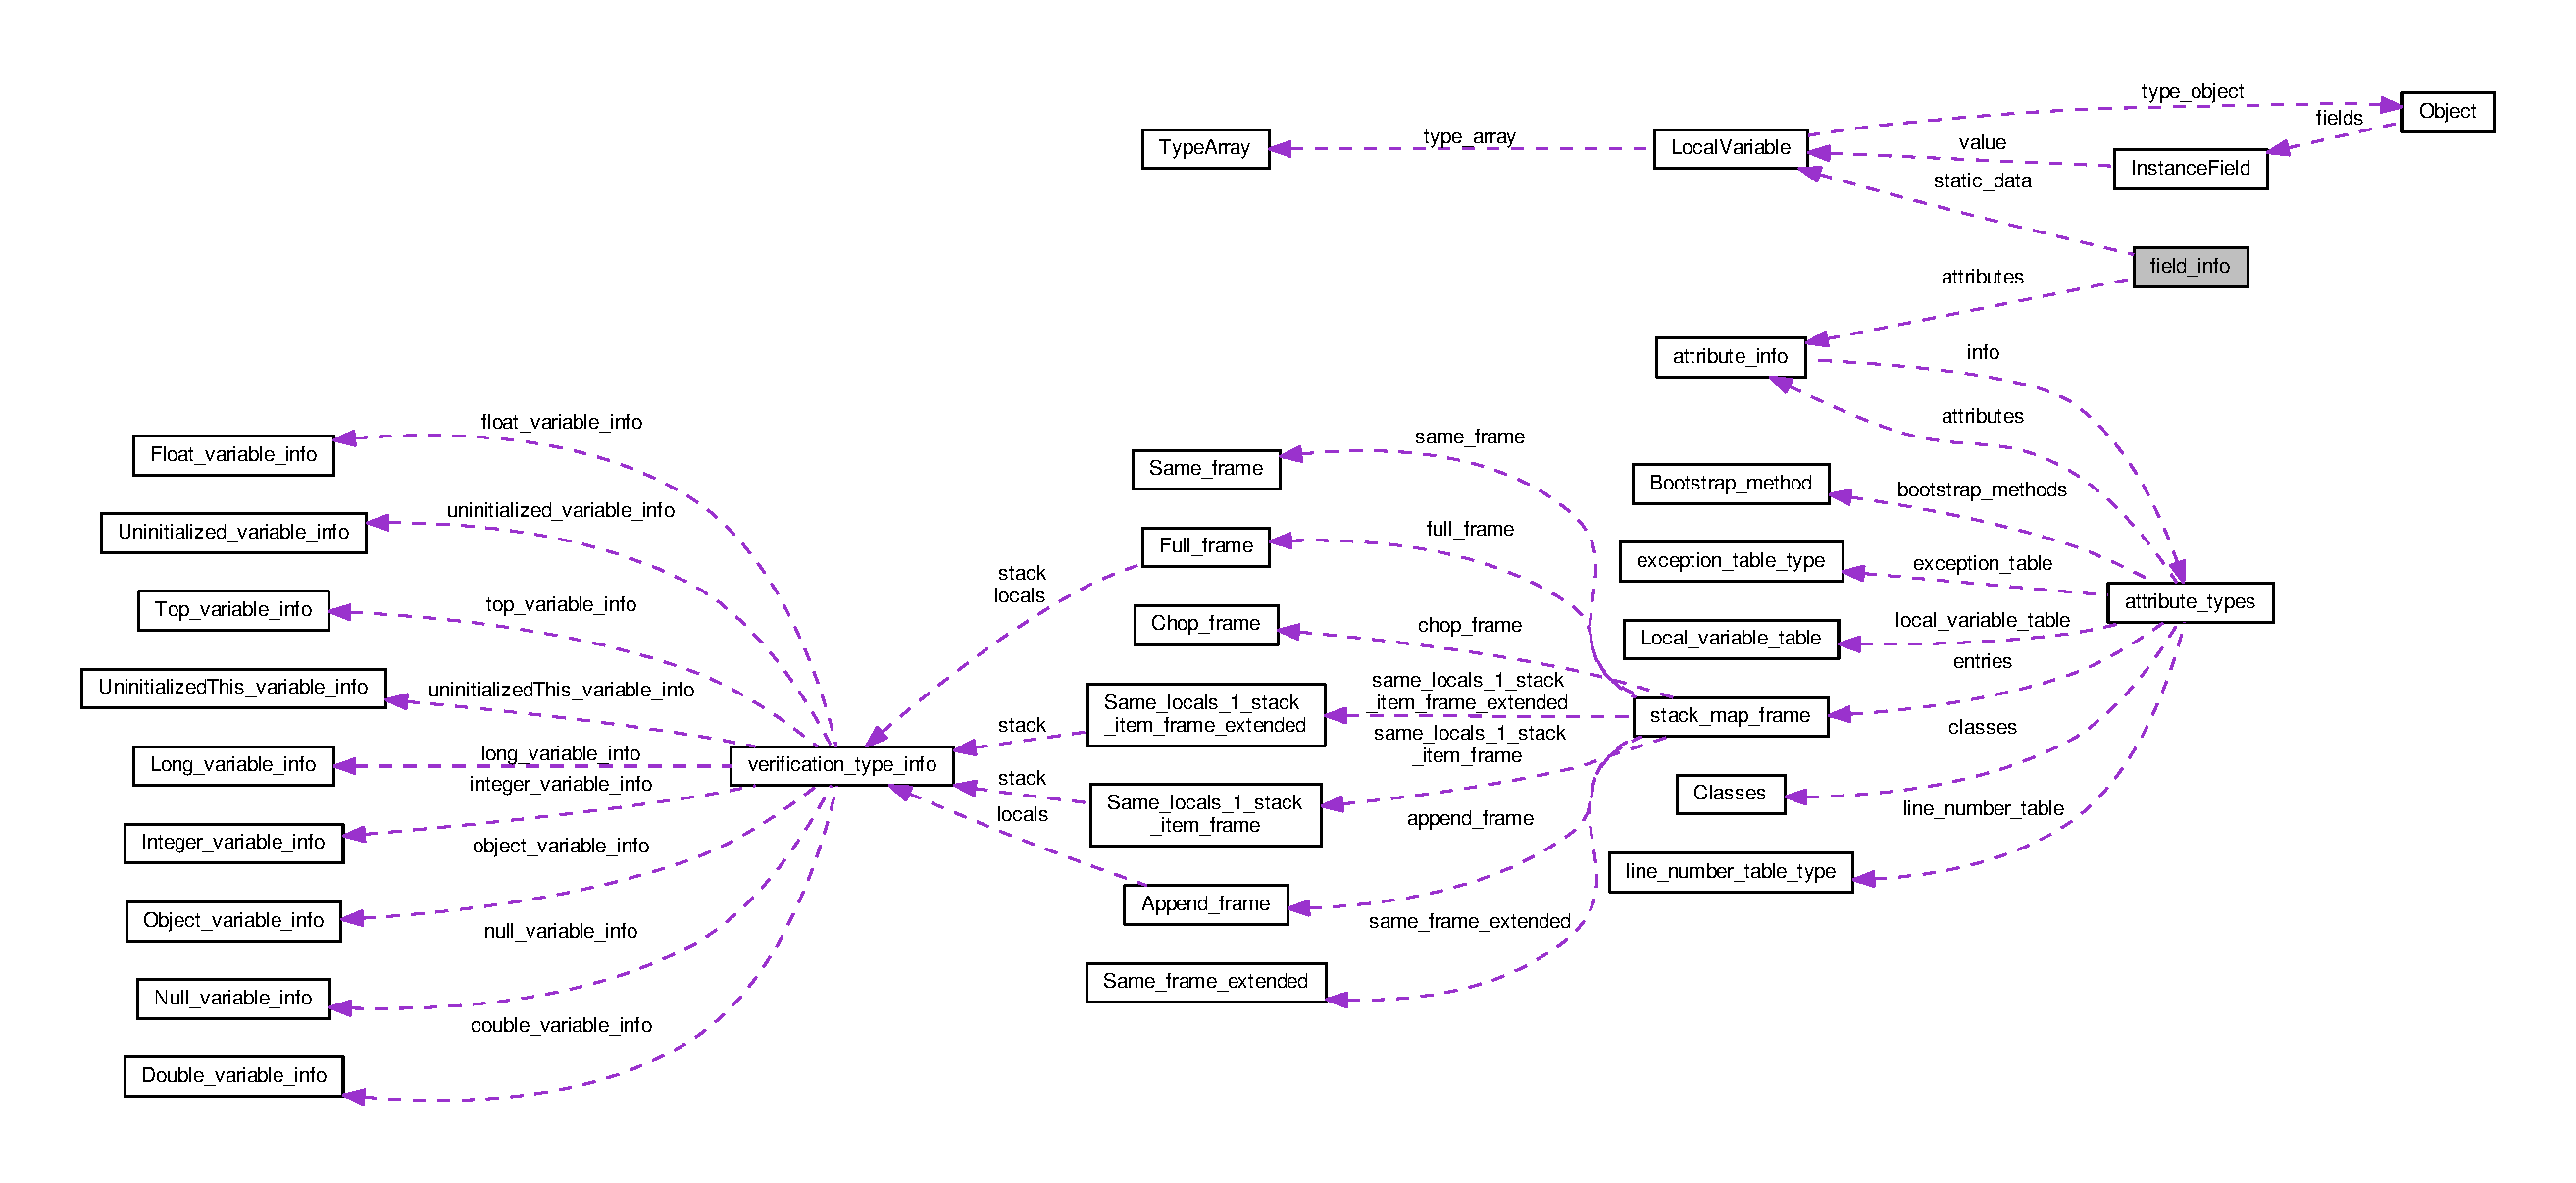
\includegraphics[width=350pt]{structfield__info__coll__graph}
\end{center}
\end{figure}
\subsection*{Public Attributes}
\begin{DoxyCompactItemize}
\item 
\hyperlink{structures_8h_a55ef8d87fd202b8417704c089899c5b9}{u2} \hyperlink{structfield__info_aa622dc9a5b5353d2f3eb2f416dacab4b}{access\+\_\+flags}
\item 
\hyperlink{structures_8h_a55ef8d87fd202b8417704c089899c5b9}{u2} \hyperlink{structfield__info_a425e3ae85badd81c67ef00acca85ad9e}{name\+\_\+index}
\item 
\hyperlink{structures_8h_a55ef8d87fd202b8417704c089899c5b9}{u2} \hyperlink{structfield__info_a12dd492b7fb1d61da1ac14938d97b07f}{descriptor\+\_\+index}
\item 
\hyperlink{structures_8h_a55ef8d87fd202b8417704c089899c5b9}{u2} \hyperlink{structfield__info_a83bfa4ff84a608e3dbd1c3968ebe1b80}{attributes\+\_\+count}
\item 
\hyperlink{structattribute__info}{attribute\+\_\+info} $\ast$ \hyperlink{structfield__info_afdda114944ae5eaae78c237f99257108}{attributes}
\item 
\hyperlink{structLocalVariable}{Local\+Variable} $\ast$ \hyperlink{structfield__info_a90fc91c18e08fe2325cdeded20ee4578}{static\+\_\+data}
\end{DoxyCompactItemize}


\subsection{Member Data Documentation}
\index{field\+\_\+info@{field\+\_\+info}!access\+\_\+flags@{access\+\_\+flags}}
\index{access\+\_\+flags@{access\+\_\+flags}!field\+\_\+info@{field\+\_\+info}}
\subsubsection[{\texorpdfstring{access\+\_\+flags}{access_flags}}]{\setlength{\rightskip}{0pt plus 5cm}{\bf u2} field\+\_\+info\+::access\+\_\+flags}\hypertarget{structfield__info_aa622dc9a5b5353d2f3eb2f416dacab4b}{}\label{structfield__info_aa622dc9a5b5353d2f3eb2f416dacab4b}
\index{field\+\_\+info@{field\+\_\+info}!attributes@{attributes}}
\index{attributes@{attributes}!field\+\_\+info@{field\+\_\+info}}
\subsubsection[{\texorpdfstring{attributes}{attributes}}]{\setlength{\rightskip}{0pt plus 5cm}{\bf attribute\+\_\+info}$\ast$ field\+\_\+info\+::attributes}\hypertarget{structfield__info_afdda114944ae5eaae78c237f99257108}{}\label{structfield__info_afdda114944ae5eaae78c237f99257108}
\index{field\+\_\+info@{field\+\_\+info}!attributes\+\_\+count@{attributes\+\_\+count}}
\index{attributes\+\_\+count@{attributes\+\_\+count}!field\+\_\+info@{field\+\_\+info}}
\subsubsection[{\texorpdfstring{attributes\+\_\+count}{attributes_count}}]{\setlength{\rightskip}{0pt plus 5cm}{\bf u2} field\+\_\+info\+::attributes\+\_\+count}\hypertarget{structfield__info_a83bfa4ff84a608e3dbd1c3968ebe1b80}{}\label{structfield__info_a83bfa4ff84a608e3dbd1c3968ebe1b80}
\index{field\+\_\+info@{field\+\_\+info}!descriptor\+\_\+index@{descriptor\+\_\+index}}
\index{descriptor\+\_\+index@{descriptor\+\_\+index}!field\+\_\+info@{field\+\_\+info}}
\subsubsection[{\texorpdfstring{descriptor\+\_\+index}{descriptor_index}}]{\setlength{\rightskip}{0pt plus 5cm}{\bf u2} field\+\_\+info\+::descriptor\+\_\+index}\hypertarget{structfield__info_a12dd492b7fb1d61da1ac14938d97b07f}{}\label{structfield__info_a12dd492b7fb1d61da1ac14938d97b07f}
\index{field\+\_\+info@{field\+\_\+info}!name\+\_\+index@{name\+\_\+index}}
\index{name\+\_\+index@{name\+\_\+index}!field\+\_\+info@{field\+\_\+info}}
\subsubsection[{\texorpdfstring{name\+\_\+index}{name_index}}]{\setlength{\rightskip}{0pt plus 5cm}{\bf u2} field\+\_\+info\+::name\+\_\+index}\hypertarget{structfield__info_a425e3ae85badd81c67ef00acca85ad9e}{}\label{structfield__info_a425e3ae85badd81c67ef00acca85ad9e}
\index{field\+\_\+info@{field\+\_\+info}!static\+\_\+data@{static\+\_\+data}}
\index{static\+\_\+data@{static\+\_\+data}!field\+\_\+info@{field\+\_\+info}}
\subsubsection[{\texorpdfstring{static\+\_\+data}{static_data}}]{\setlength{\rightskip}{0pt plus 5cm}{\bf Local\+Variable}$\ast$ field\+\_\+info\+::static\+\_\+data}\hypertarget{structfield__info_a90fc91c18e08fe2325cdeded20ee4578}{}\label{structfield__info_a90fc91c18e08fe2325cdeded20ee4578}


The documentation for this struct was generated from the following file\+:\begin{DoxyCompactItemize}
\item 
\hyperlink{structures_8h}{structures.\+h}\end{DoxyCompactItemize}

\hypertarget{structFloat__variable__info}{}\section{Float\+\_\+variable\+\_\+info Struct Reference}
\label{structFloat__variable__info}\index{Float\+\_\+variable\+\_\+info@{Float\+\_\+variable\+\_\+info}}


{\ttfamily \#include $<$structures.\+h$>$}



The documentation for this struct was generated from the following file\+:\begin{DoxyCompactItemize}
\item 
\hyperlink{structures_8h}{structures.\+h}\end{DoxyCompactItemize}

\hypertarget{structFrame}{}\section{Frame Struct Reference}
\label{structFrame}\index{Frame@{Frame}}


{\ttfamily \#include $<$frame.\+h$>$}



Collaboration diagram for Frame\+:
% FIG 0
\subsection*{Public Attributes}
\begin{DoxyCompactItemize}
\item 
\hyperlink{structures_8h_ae391a1d79bb0c8cbc283f0283e3c098b}{u4} \hyperlink{structFrame_ada6a6cf76d00cbadf43a86a686dd026c}{pc}
\item 
\hyperlink{structmethod__info}{method\+\_\+info} $\ast$ \hyperlink{structFrame_af0943cac72b53aa5aa67f3e7097430a1}{method}
\item 
\hyperlink{structcp__info}{cp\+\_\+info} $\ast$ \hyperlink{structFrame_ada1bd832b6f72f87a35d88c68b9a188a}{cp}
\item 
\hyperlink{structLocalVariable}{Local\+Variable} $\ast$ \hyperlink{structFrame_a1a3968ae645e9c154229a2631639ebd5}{local\+\_\+variables}
\item 
\hyperlink{structStackOperand}{Stack\+Operand} $\ast$ \hyperlink{structFrame_ab311fc7762ab460f039e58b024c4d229}{operands}
\item 
\hyperlink{structures_8h_a64f8055b64cf2a4c299c841130c5c938}{u1} $\ast$ \hyperlink{structFrame_ad3bdd8cc30352e62af5898b699d54c16}{bytecode}
\end{DoxyCompactItemize}


\subsection{Member Data Documentation}
\index{Frame@{Frame}!bytecode@{bytecode}}
\index{bytecode@{bytecode}!Frame@{Frame}}
\subsubsection[{\texorpdfstring{bytecode}{bytecode}}]{\setlength{\rightskip}{0pt plus 5cm}{\bf u1}$\ast$ Frame\+::bytecode}\hypertarget{structFrame_ad3bdd8cc30352e62af5898b699d54c16}{}\label{structFrame_ad3bdd8cc30352e62af5898b699d54c16}
\index{Frame@{Frame}!cp@{cp}}
\index{cp@{cp}!Frame@{Frame}}
\subsubsection[{\texorpdfstring{cp}{cp}}]{\setlength{\rightskip}{0pt plus 5cm}{\bf cp\+\_\+info}$\ast$ Frame\+::cp}\hypertarget{structFrame_ada1bd832b6f72f87a35d88c68b9a188a}{}\label{structFrame_ada1bd832b6f72f87a35d88c68b9a188a}
\index{Frame@{Frame}!local\+\_\+variables@{local\+\_\+variables}}
\index{local\+\_\+variables@{local\+\_\+variables}!Frame@{Frame}}
\subsubsection[{\texorpdfstring{local\+\_\+variables}{local_variables}}]{\setlength{\rightskip}{0pt plus 5cm}{\bf Local\+Variable}$\ast$ Frame\+::local\+\_\+variables}\hypertarget{structFrame_a1a3968ae645e9c154229a2631639ebd5}{}\label{structFrame_a1a3968ae645e9c154229a2631639ebd5}
\index{Frame@{Frame}!method@{method}}
\index{method@{method}!Frame@{Frame}}
\subsubsection[{\texorpdfstring{method}{method}}]{\setlength{\rightskip}{0pt plus 5cm}{\bf method\+\_\+info}$\ast$ Frame\+::method}\hypertarget{structFrame_af0943cac72b53aa5aa67f3e7097430a1}{}\label{structFrame_af0943cac72b53aa5aa67f3e7097430a1}
\index{Frame@{Frame}!operands@{operands}}
\index{operands@{operands}!Frame@{Frame}}
\subsubsection[{\texorpdfstring{operands}{operands}}]{\setlength{\rightskip}{0pt plus 5cm}{\bf Stack\+Operand}$\ast$ Frame\+::operands}\hypertarget{structFrame_ab311fc7762ab460f039e58b024c4d229}{}\label{structFrame_ab311fc7762ab460f039e58b024c4d229}
\index{Frame@{Frame}!pc@{pc}}
\index{pc@{pc}!Frame@{Frame}}
\subsubsection[{\texorpdfstring{pc}{pc}}]{\setlength{\rightskip}{0pt plus 5cm}{\bf u4} Frame\+::pc}\hypertarget{structFrame_ada6a6cf76d00cbadf43a86a686dd026c}{}\label{structFrame_ada6a6cf76d00cbadf43a86a686dd026c}


The documentation for this struct was generated from the following file\+:\begin{DoxyCompactItemize}
\item 
\hyperlink{frame_8h}{frame.\+h}\end{DoxyCompactItemize}

\hypertarget{structFull__frame}{}\section{Full\+\_\+frame Struct Reference}
\label{structFull__frame}\index{Full\+\_\+frame@{Full\+\_\+frame}}


{\ttfamily \#include $<$structures.\+h$>$}



Collaboration diagram for Full\+\_\+frame\+:
% FIG 0
\subsection*{Public Attributes}
\begin{DoxyCompactItemize}
\item 
\hyperlink{structures_8h_a55ef8d87fd202b8417704c089899c5b9}{u2} \hyperlink{structFull__frame_a2f561b5115209c671be0395a95a53dd5}{offset\+\_\+delta}
\item 
\hyperlink{structures_8h_a55ef8d87fd202b8417704c089899c5b9}{u2} \hyperlink{structFull__frame_a71a6efd7eaea7f6eb0ad1de7c70b4245}{number\+\_\+of\+\_\+locals}
\item 
\hyperlink{structverification__type__info}{verification\+\_\+type\+\_\+info} $\ast$ \hyperlink{structFull__frame_a12b01bc78373d145cbae4553a7c9b6a5}{locals}
\item 
\hyperlink{structures_8h_a55ef8d87fd202b8417704c089899c5b9}{u2} \hyperlink{structFull__frame_a11b6e1548b1ca3c416abc3fa6c3d3935}{number\+\_\+of\+\_\+stack\+\_\+items}
\item 
\hyperlink{structverification__type__info}{verification\+\_\+type\+\_\+info} $\ast$ \hyperlink{structFull__frame_a40ff4ea967461300e1ce8dbb51e28fa0}{stack}
\end{DoxyCompactItemize}


\subsection{Member Data Documentation}
\index{Full\+\_\+frame@{Full\+\_\+frame}!locals@{locals}}
\index{locals@{locals}!Full\+\_\+frame@{Full\+\_\+frame}}
\subsubsection[{\texorpdfstring{locals}{locals}}]{\setlength{\rightskip}{0pt plus 5cm}{\bf verification\+\_\+type\+\_\+info}$\ast$ Full\+\_\+frame\+::locals}\hypertarget{structFull__frame_a12b01bc78373d145cbae4553a7c9b6a5}{}\label{structFull__frame_a12b01bc78373d145cbae4553a7c9b6a5}
\index{Full\+\_\+frame@{Full\+\_\+frame}!number\+\_\+of\+\_\+locals@{number\+\_\+of\+\_\+locals}}
\index{number\+\_\+of\+\_\+locals@{number\+\_\+of\+\_\+locals}!Full\+\_\+frame@{Full\+\_\+frame}}
\subsubsection[{\texorpdfstring{number\+\_\+of\+\_\+locals}{number_of_locals}}]{\setlength{\rightskip}{0pt plus 5cm}{\bf u2} Full\+\_\+frame\+::number\+\_\+of\+\_\+locals}\hypertarget{structFull__frame_a71a6efd7eaea7f6eb0ad1de7c70b4245}{}\label{structFull__frame_a71a6efd7eaea7f6eb0ad1de7c70b4245}
\index{Full\+\_\+frame@{Full\+\_\+frame}!number\+\_\+of\+\_\+stack\+\_\+items@{number\+\_\+of\+\_\+stack\+\_\+items}}
\index{number\+\_\+of\+\_\+stack\+\_\+items@{number\+\_\+of\+\_\+stack\+\_\+items}!Full\+\_\+frame@{Full\+\_\+frame}}
\subsubsection[{\texorpdfstring{number\+\_\+of\+\_\+stack\+\_\+items}{number_of_stack_items}}]{\setlength{\rightskip}{0pt plus 5cm}{\bf u2} Full\+\_\+frame\+::number\+\_\+of\+\_\+stack\+\_\+items}\hypertarget{structFull__frame_a11b6e1548b1ca3c416abc3fa6c3d3935}{}\label{structFull__frame_a11b6e1548b1ca3c416abc3fa6c3d3935}
\index{Full\+\_\+frame@{Full\+\_\+frame}!offset\+\_\+delta@{offset\+\_\+delta}}
\index{offset\+\_\+delta@{offset\+\_\+delta}!Full\+\_\+frame@{Full\+\_\+frame}}
\subsubsection[{\texorpdfstring{offset\+\_\+delta}{offset_delta}}]{\setlength{\rightskip}{0pt plus 5cm}{\bf u2} Full\+\_\+frame\+::offset\+\_\+delta}\hypertarget{structFull__frame_a2f561b5115209c671be0395a95a53dd5}{}\label{structFull__frame_a2f561b5115209c671be0395a95a53dd5}
\index{Full\+\_\+frame@{Full\+\_\+frame}!stack@{stack}}
\index{stack@{stack}!Full\+\_\+frame@{Full\+\_\+frame}}
\subsubsection[{\texorpdfstring{stack}{stack}}]{\setlength{\rightskip}{0pt plus 5cm}{\bf verification\+\_\+type\+\_\+info}$\ast$ Full\+\_\+frame\+::stack}\hypertarget{structFull__frame_a40ff4ea967461300e1ce8dbb51e28fa0}{}\label{structFull__frame_a40ff4ea967461300e1ce8dbb51e28fa0}


The documentation for this struct was generated from the following file\+:\begin{DoxyCompactItemize}
\item 
\hyperlink{structures_8h}{structures.\+h}\end{DoxyCompactItemize}

\hypertarget{structInteger__variable__info}{}\section{Integer\+\_\+variable\+\_\+info Struct Reference}
\label{structInteger__variable__info}\index{Integer\+\_\+variable\+\_\+info@{Integer\+\_\+variable\+\_\+info}}


The documentation for this struct was generated from the following file\+:\begin{DoxyCompactItemize}
\item 
structures.\+h\end{DoxyCompactItemize}

\hypertarget{structJVM}{}\section{J\+VM Struct Reference}
\label{structJVM}\index{J\+VM@{J\+VM}}


{\ttfamily \#include $<$jvm.\+h$>$}

\subsection*{Public Attributes}
\begin{DoxyCompactItemize}
\item 
\hyperlink{structures_8h_ae391a1d79bb0c8cbc283f0283e3c098b}{u4} \hyperlink{structJVM_aeacbab6a3ba9b278832add772ad82a19}{pc}
\end{DoxyCompactItemize}


\subsection{Member Data Documentation}
\index{J\+VM@{J\+VM}!pc@{pc}}
\index{pc@{pc}!J\+VM@{J\+VM}}
\subsubsection[{\texorpdfstring{pc}{pc}}]{\setlength{\rightskip}{0pt plus 5cm}{\bf u4} J\+V\+M\+::pc}\hypertarget{structJVM_aeacbab6a3ba9b278832add772ad82a19}{}\label{structJVM_aeacbab6a3ba9b278832add772ad82a19}


The documentation for this struct was generated from the following file\+:\begin{DoxyCompactItemize}
\item 
\hyperlink{jvm_8h}{jvm.\+h}\end{DoxyCompactItemize}

\hypertarget{structline__number__table__type}{}\section{line\+\_\+number\+\_\+table\+\_\+type Struct Reference}
\label{structline__number__table__type}\index{line\+\_\+number\+\_\+table\+\_\+type@{line\+\_\+number\+\_\+table\+\_\+type}}


{\ttfamily \#include $<$structures.\+h$>$}

\subsection*{Public Attributes}
\begin{DoxyCompactItemize}
\item 
\hyperlink{structures_8h_a55ef8d87fd202b8417704c089899c5b9}{u2} \hyperlink{structline__number__table__type_ac0e263d3f0484fb8bea365e8b87398e1}{start\+\_\+pc}
\item 
\hyperlink{structures_8h_a55ef8d87fd202b8417704c089899c5b9}{u2} \hyperlink{structline__number__table__type_ac9f2fe3d86343b8eb013f969fa31314c}{line\+\_\+number}
\end{DoxyCompactItemize}


\subsection{Member Data Documentation}
\index{line\+\_\+number\+\_\+table\+\_\+type@{line\+\_\+number\+\_\+table\+\_\+type}!line\+\_\+number@{line\+\_\+number}}
\index{line\+\_\+number@{line\+\_\+number}!line\+\_\+number\+\_\+table\+\_\+type@{line\+\_\+number\+\_\+table\+\_\+type}}
\subsubsection[{\texorpdfstring{line\+\_\+number}{line_number}}]{\setlength{\rightskip}{0pt plus 5cm}{\bf u2} line\+\_\+number\+\_\+table\+\_\+type\+::line\+\_\+number}\hypertarget{structline__number__table__type_ac9f2fe3d86343b8eb013f969fa31314c}{}\label{structline__number__table__type_ac9f2fe3d86343b8eb013f969fa31314c}
\index{line\+\_\+number\+\_\+table\+\_\+type@{line\+\_\+number\+\_\+table\+\_\+type}!start\+\_\+pc@{start\+\_\+pc}}
\index{start\+\_\+pc@{start\+\_\+pc}!line\+\_\+number\+\_\+table\+\_\+type@{line\+\_\+number\+\_\+table\+\_\+type}}
\subsubsection[{\texorpdfstring{start\+\_\+pc}{start_pc}}]{\setlength{\rightskip}{0pt plus 5cm}{\bf u2} line\+\_\+number\+\_\+table\+\_\+type\+::start\+\_\+pc}\hypertarget{structline__number__table__type_ac0e263d3f0484fb8bea365e8b87398e1}{}\label{structline__number__table__type_ac0e263d3f0484fb8bea365e8b87398e1}


The documentation for this struct was generated from the following file\+:\begin{DoxyCompactItemize}
\item 
\hyperlink{structures_8h}{structures.\+h}\end{DoxyCompactItemize}

\hypertarget{structLocal__variable__table}{}\section{Local\+\_\+variable\+\_\+table Struct Reference}
\label{structLocal__variable__table}\index{Local\+\_\+variable\+\_\+table@{Local\+\_\+variable\+\_\+table}}
\subsection*{Public Attributes}
\begin{DoxyCompactItemize}
\item 
u2 {\bfseries start\+\_\+pc}\hypertarget{structLocal__variable__table_a857ab3f5a0d3a22f1eb7eccdd9c034e1}{}\label{structLocal__variable__table_a857ab3f5a0d3a22f1eb7eccdd9c034e1}

\item 
u2 {\bfseries length}\hypertarget{structLocal__variable__table_aa7ed2c337f001f6922abef82a7a2877b}{}\label{structLocal__variable__table_aa7ed2c337f001f6922abef82a7a2877b}

\item 
u2 {\bfseries name\+\_\+index}\hypertarget{structLocal__variable__table_ae14ab32d3cf126ede896ea6b1a7053a2}{}\label{structLocal__variable__table_ae14ab32d3cf126ede896ea6b1a7053a2}

\item 
u2 {\bfseries descriptor\+\_\+index}\hypertarget{structLocal__variable__table_ac30f0857c677e82b9665b709369adb5c}{}\label{structLocal__variable__table_ac30f0857c677e82b9665b709369adb5c}

\item 
u2 {\bfseries index}\hypertarget{structLocal__variable__table_aa9c60b3758f3edc8c4761af238e576a9}{}\label{structLocal__variable__table_aa9c60b3758f3edc8c4761af238e576a9}

\end{DoxyCompactItemize}


The documentation for this struct was generated from the following file\+:\begin{DoxyCompactItemize}
\item 
structures.\+h\end{DoxyCompactItemize}

\hypertarget{structLocalVariable}{}\section{Local\+Variable Struct Reference}
\label{structLocalVariable}\index{Local\+Variable@{Local\+Variable}}


{\ttfamily \#include $<$structures.\+h$>$}



Collaboration diagram for Local\+Variable\+:
% FIG 0
\subsection*{Public Attributes}
\begin{DoxyCompactItemize}
\item 
\hyperlink{structures_8h_a64f8055b64cf2a4c299c841130c5c938}{u1} \hyperlink{structLocalVariable_a05438f40d41a69cde0a4d50a37bf9420}{type}
\item 
\begin{tabbing}
xx\=xx\=xx\=xx\=xx\=xx\=xx\=xx\=xx\=\kill
union \{\\
\>\hyperlink{structures_8h_ae391a1d79bb0c8cbc283f0283e3c098b}{u4} \hyperlink{structLocalVariable_aee58138d840bf24f71cd8c4fd2f84db7}{value}\\
\>uint64\_t \hyperlink{structLocalVariable_af14e5709d8a7c9397571316821b9171b}{type\_long}\\
\>uint64\_t \hyperlink{structLocalVariable_a488dfde0ac92dbb3f2b4d56280771141}{type\_double}\\
\>\hyperlink{structTypeArray}{TypeArray} \hyperlink{structLocalVariable_a6905d4b07d1ff41deaa0189ae8761850}{type\_array}\\
\}; \\

\end{tabbing}\end{DoxyCompactItemize}


\subsection{Member Data Documentation}
\subsubsection[{\texorpdfstring{"@36}{@36}}]{\setlength{\rightskip}{0pt plus 5cm}union \{ ... \} }\hypertarget{structLocalVariable_a3570d34d2fed3081d2b7a21bb07cf290}{}\label{structLocalVariable_a3570d34d2fed3081d2b7a21bb07cf290}
\index{Local\+Variable@{Local\+Variable}!type@{type}}
\index{type@{type}!Local\+Variable@{Local\+Variable}}
\subsubsection[{\texorpdfstring{type}{type}}]{\setlength{\rightskip}{0pt plus 5cm}{\bf u1} Local\+Variable\+::type}\hypertarget{structLocalVariable_a05438f40d41a69cde0a4d50a37bf9420}{}\label{structLocalVariable_a05438f40d41a69cde0a4d50a37bf9420}
\index{Local\+Variable@{Local\+Variable}!type\+\_\+array@{type\+\_\+array}}
\index{type\+\_\+array@{type\+\_\+array}!Local\+Variable@{Local\+Variable}}
\subsubsection[{\texorpdfstring{type\+\_\+array}{type_array}}]{\setlength{\rightskip}{0pt plus 5cm}{\bf Type\+Array} Local\+Variable\+::type\+\_\+array}\hypertarget{structLocalVariable_a6905d4b07d1ff41deaa0189ae8761850}{}\label{structLocalVariable_a6905d4b07d1ff41deaa0189ae8761850}
\index{Local\+Variable@{Local\+Variable}!type\+\_\+double@{type\+\_\+double}}
\index{type\+\_\+double@{type\+\_\+double}!Local\+Variable@{Local\+Variable}}
\subsubsection[{\texorpdfstring{type\+\_\+double}{type_double}}]{\setlength{\rightskip}{0pt plus 5cm}uint64\+\_\+t Local\+Variable\+::type\+\_\+double}\hypertarget{structLocalVariable_a488dfde0ac92dbb3f2b4d56280771141}{}\label{structLocalVariable_a488dfde0ac92dbb3f2b4d56280771141}
\index{Local\+Variable@{Local\+Variable}!type\+\_\+long@{type\+\_\+long}}
\index{type\+\_\+long@{type\+\_\+long}!Local\+Variable@{Local\+Variable}}
\subsubsection[{\texorpdfstring{type\+\_\+long}{type_long}}]{\setlength{\rightskip}{0pt plus 5cm}uint64\+\_\+t Local\+Variable\+::type\+\_\+long}\hypertarget{structLocalVariable_af14e5709d8a7c9397571316821b9171b}{}\label{structLocalVariable_af14e5709d8a7c9397571316821b9171b}
\index{Local\+Variable@{Local\+Variable}!value@{value}}
\index{value@{value}!Local\+Variable@{Local\+Variable}}
\subsubsection[{\texorpdfstring{value}{value}}]{\setlength{\rightskip}{0pt plus 5cm}{\bf u4} Local\+Variable\+::value}\hypertarget{structLocalVariable_aee58138d840bf24f71cd8c4fd2f84db7}{}\label{structLocalVariable_aee58138d840bf24f71cd8c4fd2f84db7}


The documentation for this struct was generated from the following file\+:\begin{DoxyCompactItemize}
\item 
\hyperlink{structures_8h}{structures.\+h}\end{DoxyCompactItemize}

\hypertarget{structLong__variable__info}{}\section{Long\+\_\+variable\+\_\+info Struct Reference}
\label{structLong__variable__info}\index{Long\+\_\+variable\+\_\+info@{Long\+\_\+variable\+\_\+info}}


The documentation for this struct was generated from the following file\+:\begin{DoxyCompactItemize}
\item 
structures.\+h\end{DoxyCompactItemize}

\hypertarget{structMethod}{}\section{Method Struct Reference}
\label{structMethod}\index{Method@{Method}}


Collaboration diagram for Method\+:
% FIG 0
\subsection*{Public Attributes}
\begin{DoxyCompactItemize}
\item 
\hyperlink{structClassFile}{Class\+File} $\ast$ {\bfseries classes\+\_\+arr} \mbox{[}20\mbox{]}\hypertarget{structMethod_ace741cd234df7db5849ee2af75870b8c}{}\label{structMethod_ace741cd234df7db5849ee2af75870b8c}

\item 
u2 {\bfseries num\+\_\+classes}\hypertarget{structMethod_a40dccf4ca5a8d3a74798917a888be720}{}\label{structMethod_a40dccf4ca5a8d3a74798917a888be720}

\end{DoxyCompactItemize}


The documentation for this struct was generated from the following file\+:\begin{DoxyCompactItemize}
\item 
structures.\+h\end{DoxyCompactItemize}

\hypertarget{structmethod__info}{}\section{method\+\_\+info Struct Reference}
\label{structmethod__info}\index{method\+\_\+info@{method\+\_\+info}}


Collaboration diagram for method\+\_\+info\+:
% FIG 0
\subsection*{Public Attributes}
\begin{DoxyCompactItemize}
\item 
u2 {\bfseries access\+\_\+flags}\hypertarget{structmethod__info_a3b657027a141cdbc94ded28607c98be5}{}\label{structmethod__info_a3b657027a141cdbc94ded28607c98be5}

\item 
u2 {\bfseries name\+\_\+index}\hypertarget{structmethod__info_ab91d62d0658b77bba83f6bb685e3bbb9}{}\label{structmethod__info_ab91d62d0658b77bba83f6bb685e3bbb9}

\item 
u2 {\bfseries descriptor\+\_\+index}\hypertarget{structmethod__info_a7713103e0c8d060630ad62774fb9be37}{}\label{structmethod__info_a7713103e0c8d060630ad62774fb9be37}

\item 
u2 {\bfseries attributes\+\_\+count}\hypertarget{structmethod__info_ad9e5e1e2fc850806addadd6deab8565d}{}\label{structmethod__info_ad9e5e1e2fc850806addadd6deab8565d}

\item 
\hyperlink{structattribute__info}{attribute\+\_\+info} $\ast$ {\bfseries attributes}\hypertarget{structmethod__info_a8ce4caaa03680c91f548558a38647ad8}{}\label{structmethod__info_a8ce4caaa03680c91f548558a38647ad8}

\end{DoxyCompactItemize}


The documentation for this struct was generated from the following file\+:\begin{DoxyCompactItemize}
\item 
structures.\+h\end{DoxyCompactItemize}

\hypertarget{structNull__variable__info}{}\section{Null\+\_\+variable\+\_\+info Struct Reference}
\label{structNull__variable__info}\index{Null\+\_\+variable\+\_\+info@{Null\+\_\+variable\+\_\+info}}


The documentation for this struct was generated from the following file\+:\begin{DoxyCompactItemize}
\item 
structures.\+h\end{DoxyCompactItemize}

\hypertarget{structObject__variable__info}{}\section{Object\+\_\+variable\+\_\+info Struct Reference}
\label{structObject__variable__info}\index{Object\+\_\+variable\+\_\+info@{Object\+\_\+variable\+\_\+info}}
\subsection*{Public Attributes}
\begin{DoxyCompactItemize}
\item 
u2 {\bfseries cpool\+\_\+index}\hypertarget{structObject__variable__info_a0588843a5e59b67c1732ed9f6b5eb5a0}{}\label{structObject__variable__info_a0588843a5e59b67c1732ed9f6b5eb5a0}

\end{DoxyCompactItemize}


The documentation for this struct was generated from the following file\+:\begin{DoxyCompactItemize}
\item 
structures.\+h\end{DoxyCompactItemize}

\hypertarget{structop__code}{}\section{op\+\_\+code Struct Reference}
\label{structop__code}\index{op\+\_\+code@{op\+\_\+code}}


{\ttfamily \#include $<$instructions.\+h$>$}

\subsection*{Public Attributes}
\begin{DoxyCompactItemize}
\item 
uint8\+\_\+t \hyperlink{structop__code_adfbb2fc6e07e6fda7e392c0b6f6f64b6}{key}
\item 
char \hyperlink{structop__code_a0b74d91235a8b9f0a36710d68c2746d1}{value} \mbox{[}30\mbox{]}
\item 
uint8\+\_\+t \hyperlink{structop__code_ac059fd01f71776bebdc8fcccd44f7476}{arguments}
\item 
uint16\+\_\+t \hyperlink{structop__code_a8d28fff7d91873f58a4a12205dd0f8e0}{references}
\item 
void($\ast$ \hyperlink{structop__code_acd2c8c9ef3e72b9f110127c854620472}{eval} )(\hyperlink{structFrame}{Frame} $\ast$)
\end{DoxyCompactItemize}


\subsection{Member Data Documentation}
\index{op\+\_\+code@{op\+\_\+code}!arguments@{arguments}}
\index{arguments@{arguments}!op\+\_\+code@{op\+\_\+code}}
\subsubsection[{\texorpdfstring{arguments}{arguments}}]{\setlength{\rightskip}{0pt plus 5cm}uint8\+\_\+t op\+\_\+code\+::arguments}\hypertarget{structop__code_ac059fd01f71776bebdc8fcccd44f7476}{}\label{structop__code_ac059fd01f71776bebdc8fcccd44f7476}
\index{op\+\_\+code@{op\+\_\+code}!eval@{eval}}
\index{eval@{eval}!op\+\_\+code@{op\+\_\+code}}
\subsubsection[{\texorpdfstring{eval}{eval}}]{\setlength{\rightskip}{0pt plus 5cm}void($\ast$  op\+\_\+code\+::eval) ({\bf Frame} $\ast$)}\hypertarget{structop__code_acd2c8c9ef3e72b9f110127c854620472}{}\label{structop__code_acd2c8c9ef3e72b9f110127c854620472}
\index{op\+\_\+code@{op\+\_\+code}!key@{key}}
\index{key@{key}!op\+\_\+code@{op\+\_\+code}}
\subsubsection[{\texorpdfstring{key}{key}}]{\setlength{\rightskip}{0pt plus 5cm}uint8\+\_\+t op\+\_\+code\+::key}\hypertarget{structop__code_adfbb2fc6e07e6fda7e392c0b6f6f64b6}{}\label{structop__code_adfbb2fc6e07e6fda7e392c0b6f6f64b6}
\index{op\+\_\+code@{op\+\_\+code}!references@{references}}
\index{references@{references}!op\+\_\+code@{op\+\_\+code}}
\subsubsection[{\texorpdfstring{references}{references}}]{\setlength{\rightskip}{0pt plus 5cm}uint16\+\_\+t op\+\_\+code\+::references}\hypertarget{structop__code_a8d28fff7d91873f58a4a12205dd0f8e0}{}\label{structop__code_a8d28fff7d91873f58a4a12205dd0f8e0}
\index{op\+\_\+code@{op\+\_\+code}!value@{value}}
\index{value@{value}!op\+\_\+code@{op\+\_\+code}}
\subsubsection[{\texorpdfstring{value}{value}}]{\setlength{\rightskip}{0pt plus 5cm}char op\+\_\+code\+::value\mbox{[}30\mbox{]}}\hypertarget{structop__code_a0b74d91235a8b9f0a36710d68c2746d1}{}\label{structop__code_a0b74d91235a8b9f0a36710d68c2746d1}


The documentation for this struct was generated from the following file\+:\begin{DoxyCompactItemize}
\item 
\hyperlink{instructions_8h}{instructions.\+h}\end{DoxyCompactItemize}

\hypertarget{structSame__frame}{}\section{Same\+\_\+frame Struct Reference}
\label{structSame__frame}\index{Same\+\_\+frame@{Same\+\_\+frame}}


{\ttfamily \#include $<$structures.\+h$>$}



The documentation for this struct was generated from the following file\+:\begin{DoxyCompactItemize}
\item 
\hyperlink{structures_8h}{structures.\+h}\end{DoxyCompactItemize}

\hypertarget{structSame__frame__extended}{}\section{Same\+\_\+frame\+\_\+extended Struct Reference}
\label{structSame__frame__extended}\index{Same\+\_\+frame\+\_\+extended@{Same\+\_\+frame\+\_\+extended}}


{\ttfamily \#include $<$structures.\+h$>$}

\subsection*{Public Attributes}
\begin{DoxyCompactItemize}
\item 
\hyperlink{structures_8h_a55ef8d87fd202b8417704c089899c5b9}{u2} \hyperlink{structSame__frame__extended_a0305c6ff9d2d1e7b2290435c7de737c7}{offset\+\_\+delta}
\end{DoxyCompactItemize}


\subsection{Member Data Documentation}
\index{Same\+\_\+frame\+\_\+extended@{Same\+\_\+frame\+\_\+extended}!offset\+\_\+delta@{offset\+\_\+delta}}
\index{offset\+\_\+delta@{offset\+\_\+delta}!Same\+\_\+frame\+\_\+extended@{Same\+\_\+frame\+\_\+extended}}
\subsubsection[{\texorpdfstring{offset\+\_\+delta}{offset_delta}}]{\setlength{\rightskip}{0pt plus 5cm}{\bf u2} Same\+\_\+frame\+\_\+extended\+::offset\+\_\+delta}\hypertarget{structSame__frame__extended_a0305c6ff9d2d1e7b2290435c7de737c7}{}\label{structSame__frame__extended_a0305c6ff9d2d1e7b2290435c7de737c7}


The documentation for this struct was generated from the following file\+:\begin{DoxyCompactItemize}
\item 
\hyperlink{structures_8h}{structures.\+h}\end{DoxyCompactItemize}

\hypertarget{structSame__locals__1__stack__item__frame}{}\section{Same\+\_\+locals\+\_\+1\+\_\+stack\+\_\+item\+\_\+frame Struct Reference}
\label{structSame__locals__1__stack__item__frame}\index{Same\+\_\+locals\+\_\+1\+\_\+stack\+\_\+item\+\_\+frame@{Same\+\_\+locals\+\_\+1\+\_\+stack\+\_\+item\+\_\+frame}}


{\ttfamily \#include $<$structures.\+h$>$}



Collaboration diagram for Same\+\_\+locals\+\_\+1\+\_\+stack\+\_\+item\+\_\+frame\+:
\nopagebreak
\begin{figure}[H]
\begin{center}
\leavevmode
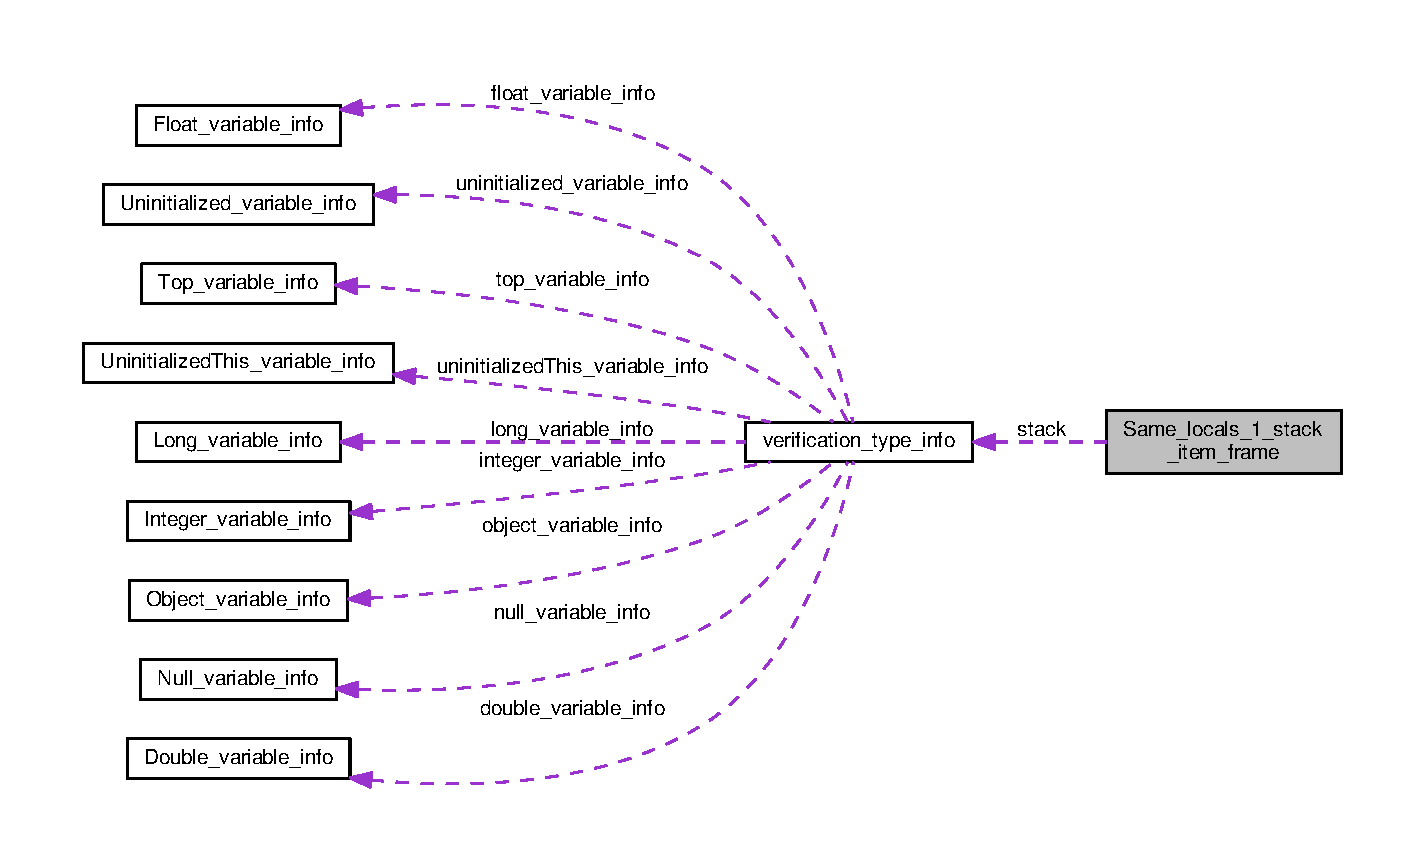
\includegraphics[width=350pt]{structSame__locals__1__stack__item__frame__coll__graph}
\end{center}
\end{figure}
\subsection*{Public Attributes}
\begin{DoxyCompactItemize}
\item 
\hyperlink{structverification__type__info}{verification\+\_\+type\+\_\+info} $\ast$ \hyperlink{structSame__locals__1__stack__item__frame_aea334c9e9f4e42aad07a6ec10a7f058a}{stack}
\end{DoxyCompactItemize}


\subsection{Member Data Documentation}
\index{Same\+\_\+locals\+\_\+1\+\_\+stack\+\_\+item\+\_\+frame@{Same\+\_\+locals\+\_\+1\+\_\+stack\+\_\+item\+\_\+frame}!stack@{stack}}
\index{stack@{stack}!Same\+\_\+locals\+\_\+1\+\_\+stack\+\_\+item\+\_\+frame@{Same\+\_\+locals\+\_\+1\+\_\+stack\+\_\+item\+\_\+frame}}
\subsubsection[{\texorpdfstring{stack}{stack}}]{\setlength{\rightskip}{0pt plus 5cm}{\bf verification\+\_\+type\+\_\+info}$\ast$ Same\+\_\+locals\+\_\+1\+\_\+stack\+\_\+item\+\_\+frame\+::stack}\hypertarget{structSame__locals__1__stack__item__frame_aea334c9e9f4e42aad07a6ec10a7f058a}{}\label{structSame__locals__1__stack__item__frame_aea334c9e9f4e42aad07a6ec10a7f058a}


The documentation for this struct was generated from the following file\+:\begin{DoxyCompactItemize}
\item 
\hyperlink{structures_8h}{structures.\+h}\end{DoxyCompactItemize}

\hypertarget{structSame__locals__1__stack__item__frame__extended}{}\section{Same\+\_\+locals\+\_\+1\+\_\+stack\+\_\+item\+\_\+frame\+\_\+extended Struct Reference}
\label{structSame__locals__1__stack__item__frame__extended}\index{Same\+\_\+locals\+\_\+1\+\_\+stack\+\_\+item\+\_\+frame\+\_\+extended@{Same\+\_\+locals\+\_\+1\+\_\+stack\+\_\+item\+\_\+frame\+\_\+extended}}


Collaboration diagram for Same\+\_\+locals\+\_\+1\+\_\+stack\+\_\+item\+\_\+frame\+\_\+extended\+:
% FIG 0
\subsection*{Public Attributes}
\begin{DoxyCompactItemize}
\item 
u2 {\bfseries offset\+\_\+delta}\hypertarget{structSame__locals__1__stack__item__frame__extended_af1fb0ce3ba68c6d6b49992b99a044235}{}\label{structSame__locals__1__stack__item__frame__extended_af1fb0ce3ba68c6d6b49992b99a044235}

\item 
\hyperlink{structverification__type__info}{verification\+\_\+type\+\_\+info} $\ast$ {\bfseries stack}\hypertarget{structSame__locals__1__stack__item__frame__extended_a7900584b7fadb413da796fbd30c1fa2b}{}\label{structSame__locals__1__stack__item__frame__extended_a7900584b7fadb413da796fbd30c1fa2b}

\end{DoxyCompactItemize}


The documentation for this struct was generated from the following file\+:\begin{DoxyCompactItemize}
\item 
structures.\+h\end{DoxyCompactItemize}

\hypertarget{structstack__map__frame}{}\section{stack\+\_\+map\+\_\+frame Struct Reference}
\label{structstack__map__frame}\index{stack\+\_\+map\+\_\+frame@{stack\+\_\+map\+\_\+frame}}


{\ttfamily \#include $<$structures.\+h$>$}



Collaboration diagram for stack\+\_\+map\+\_\+frame\+:
\nopagebreak
\begin{figure}[H]
\begin{center}
\leavevmode
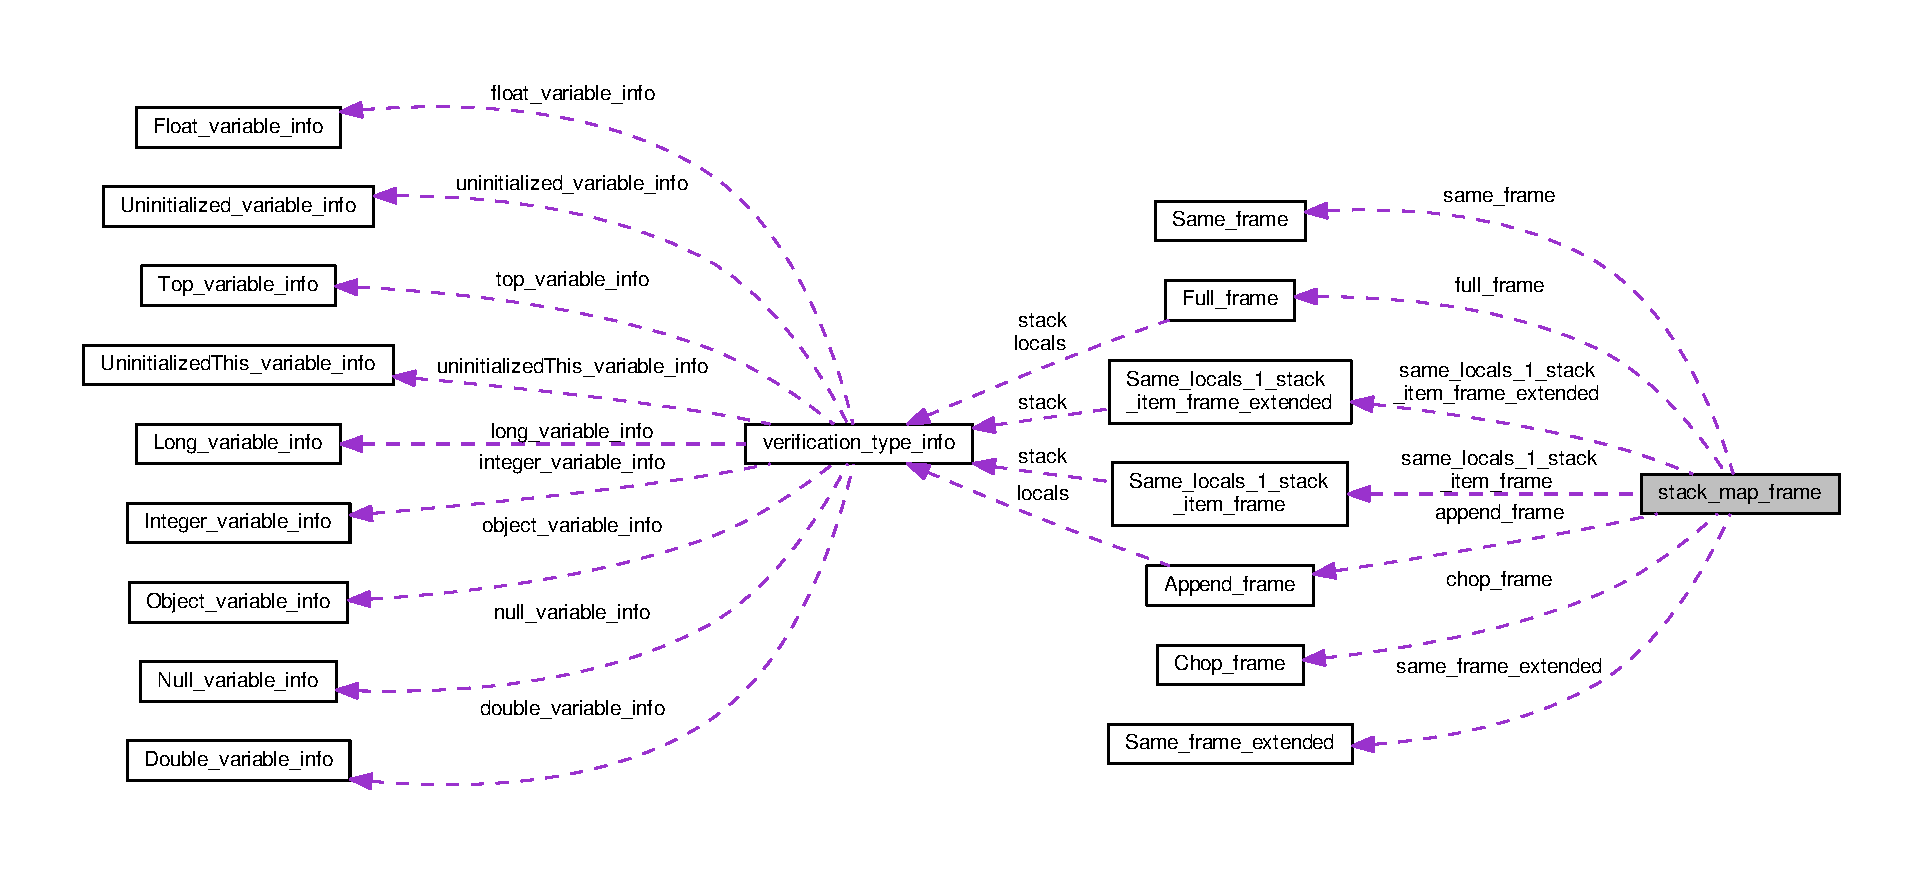
\includegraphics[width=350pt]{structstack__map__frame__coll__graph}
\end{center}
\end{figure}
\subsection*{Public Attributes}
\begin{DoxyCompactItemize}
\item 
\hyperlink{structures_8h_a64f8055b64cf2a4c299c841130c5c938}{u1} \hyperlink{structstack__map__frame_ae7d53e0f8daea6d5738a88ffb94e575c}{frame\+\_\+type}
\item 
\begin{tabbing}
xx\=xx\=xx\=xx\=xx\=xx\=xx\=xx\=xx\=\kill
union \{\\
\>\hyperlink{structSame__frame}{Same\_frame} \hyperlink{structstack__map__frame_a566369b2c76e233dc18856709be7d3dc}{same\_frame}\\
\>\hyperlink{structSame__locals__1__stack__item__frame}{Same\_locals\_1\_stack\_item\_frame} \hyperlink{structstack__map__frame_a4a73bdea158110c9c632ef657acdceed}{same\_locals\_1\_stack\_item\_frame}\\
\>\hyperlink{structSame__locals__1__stack__item__frame__extended}{Same\_locals\_1\_stack\_item\_frame\_extended} \hyperlink{structstack__map__frame_acb0262b85b6ddf629227b4e269107c4d}{same\_locals\_1\_stack\_item\_frame\_extended}\\
\>\hyperlink{structChop__frame}{Chop\_frame} \hyperlink{structstack__map__frame_a5240372d8b1af1775ee49050a515b9f2}{chop\_frame}\\
\>\hyperlink{structSame__frame__extended}{Same\_frame\_extended} \hyperlink{structstack__map__frame_a5fd4fb1c466520e7296b33ca512a844a}{same\_frame\_extended}\\
\>\hyperlink{structAppend__frame}{Append\_frame} \hyperlink{structstack__map__frame_ab412797c19922cdc0ac8fee59c59b49b}{append\_frame}\\
\>\hyperlink{structFull__frame}{Full\_frame} \hyperlink{structstack__map__frame_a6f51b3460b916cc6285c57efa37bf8e0}{full\_frame}\\
\}; \\

\end{tabbing}\end{DoxyCompactItemize}


\subsection{Member Data Documentation}
\subsubsection[{\texorpdfstring{"@23}{@23}}]{\setlength{\rightskip}{0pt plus 5cm}union \{ ... \} }\hypertarget{structstack__map__frame_a5c073aea2bad69d9058ef668105484da}{}\label{structstack__map__frame_a5c073aea2bad69d9058ef668105484da}
\index{stack\+\_\+map\+\_\+frame@{stack\+\_\+map\+\_\+frame}!append\+\_\+frame@{append\+\_\+frame}}
\index{append\+\_\+frame@{append\+\_\+frame}!stack\+\_\+map\+\_\+frame@{stack\+\_\+map\+\_\+frame}}
\subsubsection[{\texorpdfstring{append\+\_\+frame}{append_frame}}]{\setlength{\rightskip}{0pt plus 5cm}{\bf Append\+\_\+frame} stack\+\_\+map\+\_\+frame\+::append\+\_\+frame}\hypertarget{structstack__map__frame_ab412797c19922cdc0ac8fee59c59b49b}{}\label{structstack__map__frame_ab412797c19922cdc0ac8fee59c59b49b}
\index{stack\+\_\+map\+\_\+frame@{stack\+\_\+map\+\_\+frame}!chop\+\_\+frame@{chop\+\_\+frame}}
\index{chop\+\_\+frame@{chop\+\_\+frame}!stack\+\_\+map\+\_\+frame@{stack\+\_\+map\+\_\+frame}}
\subsubsection[{\texorpdfstring{chop\+\_\+frame}{chop_frame}}]{\setlength{\rightskip}{0pt plus 5cm}{\bf Chop\+\_\+frame} stack\+\_\+map\+\_\+frame\+::chop\+\_\+frame}\hypertarget{structstack__map__frame_a5240372d8b1af1775ee49050a515b9f2}{}\label{structstack__map__frame_a5240372d8b1af1775ee49050a515b9f2}
\index{stack\+\_\+map\+\_\+frame@{stack\+\_\+map\+\_\+frame}!frame\+\_\+type@{frame\+\_\+type}}
\index{frame\+\_\+type@{frame\+\_\+type}!stack\+\_\+map\+\_\+frame@{stack\+\_\+map\+\_\+frame}}
\subsubsection[{\texorpdfstring{frame\+\_\+type}{frame_type}}]{\setlength{\rightskip}{0pt plus 5cm}{\bf u1} stack\+\_\+map\+\_\+frame\+::frame\+\_\+type}\hypertarget{structstack__map__frame_ae7d53e0f8daea6d5738a88ffb94e575c}{}\label{structstack__map__frame_ae7d53e0f8daea6d5738a88ffb94e575c}
\index{stack\+\_\+map\+\_\+frame@{stack\+\_\+map\+\_\+frame}!full\+\_\+frame@{full\+\_\+frame}}
\index{full\+\_\+frame@{full\+\_\+frame}!stack\+\_\+map\+\_\+frame@{stack\+\_\+map\+\_\+frame}}
\subsubsection[{\texorpdfstring{full\+\_\+frame}{full_frame}}]{\setlength{\rightskip}{0pt plus 5cm}{\bf Full\+\_\+frame} stack\+\_\+map\+\_\+frame\+::full\+\_\+frame}\hypertarget{structstack__map__frame_a6f51b3460b916cc6285c57efa37bf8e0}{}\label{structstack__map__frame_a6f51b3460b916cc6285c57efa37bf8e0}
\index{stack\+\_\+map\+\_\+frame@{stack\+\_\+map\+\_\+frame}!same\+\_\+frame@{same\+\_\+frame}}
\index{same\+\_\+frame@{same\+\_\+frame}!stack\+\_\+map\+\_\+frame@{stack\+\_\+map\+\_\+frame}}
\subsubsection[{\texorpdfstring{same\+\_\+frame}{same_frame}}]{\setlength{\rightskip}{0pt plus 5cm}{\bf Same\+\_\+frame} stack\+\_\+map\+\_\+frame\+::same\+\_\+frame}\hypertarget{structstack__map__frame_a566369b2c76e233dc18856709be7d3dc}{}\label{structstack__map__frame_a566369b2c76e233dc18856709be7d3dc}
\index{stack\+\_\+map\+\_\+frame@{stack\+\_\+map\+\_\+frame}!same\+\_\+frame\+\_\+extended@{same\+\_\+frame\+\_\+extended}}
\index{same\+\_\+frame\+\_\+extended@{same\+\_\+frame\+\_\+extended}!stack\+\_\+map\+\_\+frame@{stack\+\_\+map\+\_\+frame}}
\subsubsection[{\texorpdfstring{same\+\_\+frame\+\_\+extended}{same_frame_extended}}]{\setlength{\rightskip}{0pt plus 5cm}{\bf Same\+\_\+frame\+\_\+extended} stack\+\_\+map\+\_\+frame\+::same\+\_\+frame\+\_\+extended}\hypertarget{structstack__map__frame_a5fd4fb1c466520e7296b33ca512a844a}{}\label{structstack__map__frame_a5fd4fb1c466520e7296b33ca512a844a}
\index{stack\+\_\+map\+\_\+frame@{stack\+\_\+map\+\_\+frame}!same\+\_\+locals\+\_\+1\+\_\+stack\+\_\+item\+\_\+frame@{same\+\_\+locals\+\_\+1\+\_\+stack\+\_\+item\+\_\+frame}}
\index{same\+\_\+locals\+\_\+1\+\_\+stack\+\_\+item\+\_\+frame@{same\+\_\+locals\+\_\+1\+\_\+stack\+\_\+item\+\_\+frame}!stack\+\_\+map\+\_\+frame@{stack\+\_\+map\+\_\+frame}}
\subsubsection[{\texorpdfstring{same\+\_\+locals\+\_\+1\+\_\+stack\+\_\+item\+\_\+frame}{same_locals_1_stack_item_frame}}]{\setlength{\rightskip}{0pt plus 5cm}{\bf Same\+\_\+locals\+\_\+1\+\_\+stack\+\_\+item\+\_\+frame} stack\+\_\+map\+\_\+frame\+::same\+\_\+locals\+\_\+1\+\_\+stack\+\_\+item\+\_\+frame}\hypertarget{structstack__map__frame_a4a73bdea158110c9c632ef657acdceed}{}\label{structstack__map__frame_a4a73bdea158110c9c632ef657acdceed}
\index{stack\+\_\+map\+\_\+frame@{stack\+\_\+map\+\_\+frame}!same\+\_\+locals\+\_\+1\+\_\+stack\+\_\+item\+\_\+frame\+\_\+extended@{same\+\_\+locals\+\_\+1\+\_\+stack\+\_\+item\+\_\+frame\+\_\+extended}}
\index{same\+\_\+locals\+\_\+1\+\_\+stack\+\_\+item\+\_\+frame\+\_\+extended@{same\+\_\+locals\+\_\+1\+\_\+stack\+\_\+item\+\_\+frame\+\_\+extended}!stack\+\_\+map\+\_\+frame@{stack\+\_\+map\+\_\+frame}}
\subsubsection[{\texorpdfstring{same\+\_\+locals\+\_\+1\+\_\+stack\+\_\+item\+\_\+frame\+\_\+extended}{same_locals_1_stack_item_frame_extended}}]{\setlength{\rightskip}{0pt plus 5cm}{\bf Same\+\_\+locals\+\_\+1\+\_\+stack\+\_\+item\+\_\+frame\+\_\+extended} stack\+\_\+map\+\_\+frame\+::same\+\_\+locals\+\_\+1\+\_\+stack\+\_\+item\+\_\+frame\+\_\+extended}\hypertarget{structstack__map__frame_acb0262b85b6ddf629227b4e269107c4d}{}\label{structstack__map__frame_acb0262b85b6ddf629227b4e269107c4d}


The documentation for this struct was generated from the following file\+:\begin{DoxyCompactItemize}
\item 
\hyperlink{structures_8h}{structures.\+h}\end{DoxyCompactItemize}

\hypertarget{structStackFrame}{}\section{Stack\+Frame Struct Reference}
\label{structStackFrame}\index{Stack\+Frame@{Stack\+Frame}}


{\ttfamily \#include $<$stack\+\_\+frame.\+h$>$}



Collaboration diagram for Stack\+Frame\+:
% FIG 0
\subsection*{Public Attributes}
\begin{DoxyCompactItemize}
\item 
\hyperlink{structFrame}{Frame} $\ast$ \hyperlink{structStackFrame_a344a354f24d9c4b6c805cd0a029100b9}{f}
\item 
struct \hyperlink{structStackFrame}{Stack\+Frame} $\ast$ \hyperlink{structStackFrame_aae670075795a607599420fd8b5181292}{pointer}
\item 
struct \hyperlink{structStackFrame}{Stack\+Frame} $\ast$ \hyperlink{structStackFrame_a9f0df83101cacbe812d0d4b3c6e08494}{top}
\end{DoxyCompactItemize}


\subsection{Member Data Documentation}
\index{Stack\+Frame@{Stack\+Frame}!f@{f}}
\index{f@{f}!Stack\+Frame@{Stack\+Frame}}
\subsubsection[{\texorpdfstring{f}{f}}]{\setlength{\rightskip}{0pt plus 5cm}{\bf Frame}$\ast$ Stack\+Frame\+::f}\hypertarget{structStackFrame_a344a354f24d9c4b6c805cd0a029100b9}{}\label{structStackFrame_a344a354f24d9c4b6c805cd0a029100b9}
\index{Stack\+Frame@{Stack\+Frame}!pointer@{pointer}}
\index{pointer@{pointer}!Stack\+Frame@{Stack\+Frame}}
\subsubsection[{\texorpdfstring{pointer}{pointer}}]{\setlength{\rightskip}{0pt plus 5cm}struct {\bf Stack\+Frame}$\ast$ Stack\+Frame\+::pointer}\hypertarget{structStackFrame_aae670075795a607599420fd8b5181292}{}\label{structStackFrame_aae670075795a607599420fd8b5181292}
\index{Stack\+Frame@{Stack\+Frame}!top@{top}}
\index{top@{top}!Stack\+Frame@{Stack\+Frame}}
\subsubsection[{\texorpdfstring{top}{top}}]{\setlength{\rightskip}{0pt plus 5cm}struct {\bf Stack\+Frame}$\ast$ Stack\+Frame\+::top}\hypertarget{structStackFrame_a9f0df83101cacbe812d0d4b3c6e08494}{}\label{structStackFrame_a9f0df83101cacbe812d0d4b3c6e08494}


The documentation for this struct was generated from the following file\+:\begin{DoxyCompactItemize}
\item 
\hyperlink{stack__frame_8h}{stack\+\_\+frame.\+h}\end{DoxyCompactItemize}

\hypertarget{structStackOperand}{}\section{Stack\+Operand Struct Reference}
\label{structStackOperand}\index{Stack\+Operand@{Stack\+Operand}}


Estrutura que representa um operando da pilha.  




{\ttfamily \#include $<$stack\+\_\+operands.\+h$>$}



Collaboration diagram for Stack\+Operand\+:
% FIG 0
\subsection*{Public Attributes}
\begin{DoxyCompactItemize}
\item 
\hyperlink{structLocalVariable}{Local\+Variable} $\ast$ \hyperlink{structStackOperand_ac2430d118d01240603507706e8a8adff}{f}
\item 
struct \hyperlink{structStackOperand}{Stack\+Operand} $\ast$ \hyperlink{structStackOperand_af4ad4c3c4e49be261c61b3856bc02b9f}{pointer}
\item 
struct \hyperlink{structStackOperand}{Stack\+Operand} $\ast$ \hyperlink{structStackOperand_a11a33c73ab08f65a14fb53af2308d052}{top}
\end{DoxyCompactItemize}


\subsection{Detailed Description}
Estrutura que representa um operando da pilha. 

Struct que implementa a pilha de operandos.

Possui um ponteiro para uma \hyperlink{structLocalVariable}{Local\+Variable} e um pointeiro para uma pilha de operandos. 

\subsection{Member Data Documentation}
\index{Stack\+Operand@{Stack\+Operand}!f@{f}}
\index{f@{f}!Stack\+Operand@{Stack\+Operand}}
\subsubsection[{\texorpdfstring{f}{f}}]{\setlength{\rightskip}{0pt plus 5cm}{\bf Local\+Variable}$\ast$ Stack\+Operand\+::f}\hypertarget{structStackOperand_ac2430d118d01240603507706e8a8adff}{}\label{structStackOperand_ac2430d118d01240603507706e8a8adff}
\index{Stack\+Operand@{Stack\+Operand}!pointer@{pointer}}
\index{pointer@{pointer}!Stack\+Operand@{Stack\+Operand}}
\subsubsection[{\texorpdfstring{pointer}{pointer}}]{\setlength{\rightskip}{0pt plus 5cm}struct {\bf Stack\+Operand}$\ast$ Stack\+Operand\+::pointer}\hypertarget{structStackOperand_af4ad4c3c4e49be261c61b3856bc02b9f}{}\label{structStackOperand_af4ad4c3c4e49be261c61b3856bc02b9f}
\index{Stack\+Operand@{Stack\+Operand}!top@{top}}
\index{top@{top}!Stack\+Operand@{Stack\+Operand}}
\subsubsection[{\texorpdfstring{top}{top}}]{\setlength{\rightskip}{0pt plus 5cm}struct {\bf Stack\+Operand}$\ast$ Stack\+Operand\+::top}\hypertarget{structStackOperand_a11a33c73ab08f65a14fb53af2308d052}{}\label{structStackOperand_a11a33c73ab08f65a14fb53af2308d052}


The documentation for this struct was generated from the following file\+:\begin{DoxyCompactItemize}
\item 
\hyperlink{stack__operands_8h}{stack\+\_\+operands.\+h}\end{DoxyCompactItemize}

\hypertarget{structTop__variable__info}{}\section{Top\+\_\+variable\+\_\+info Struct Reference}
\label{structTop__variable__info}\index{Top\+\_\+variable\+\_\+info@{Top\+\_\+variable\+\_\+info}}


{\ttfamily \#include $<$structures.\+h$>$}



The documentation for this struct was generated from the following file\+:\begin{DoxyCompactItemize}
\item 
\hyperlink{structures_8h}{structures.\+h}\end{DoxyCompactItemize}

\hypertarget{structTypeArray}{}\section{Type\+Array Struct Reference}
\label{structTypeArray}\index{Type\+Array@{Type\+Array}}


{\ttfamily \#include $<$structures.\+h$>$}

\subsection*{Public Attributes}
\begin{DoxyCompactItemize}
\item 
void $\ast$ \hyperlink{structTypeArray_a6126c1f56950b1821af98aa19d4c5cdc}{array}
\item 
\hyperlink{structures_8h_a55ef8d87fd202b8417704c089899c5b9}{u2} \hyperlink{structTypeArray_a51c37b7d51078be5f6f6dc83c58fdb22}{size}
\end{DoxyCompactItemize}


\subsection{Member Data Documentation}
\index{Type\+Array@{Type\+Array}!array@{array}}
\index{array@{array}!Type\+Array@{Type\+Array}}
\subsubsection[{\texorpdfstring{array}{array}}]{\setlength{\rightskip}{0pt plus 5cm}void$\ast$ Type\+Array\+::array}\hypertarget{structTypeArray_a6126c1f56950b1821af98aa19d4c5cdc}{}\label{structTypeArray_a6126c1f56950b1821af98aa19d4c5cdc}
\index{Type\+Array@{Type\+Array}!size@{size}}
\index{size@{size}!Type\+Array@{Type\+Array}}
\subsubsection[{\texorpdfstring{size}{size}}]{\setlength{\rightskip}{0pt plus 5cm}{\bf u2} Type\+Array\+::size}\hypertarget{structTypeArray_a51c37b7d51078be5f6f6dc83c58fdb22}{}\label{structTypeArray_a51c37b7d51078be5f6f6dc83c58fdb22}


The documentation for this struct was generated from the following file\+:\begin{DoxyCompactItemize}
\item 
\hyperlink{structures_8h}{structures.\+h}\end{DoxyCompactItemize}

\hypertarget{structUninitialized__variable__info}{}\section{Uninitialized\+\_\+variable\+\_\+info Struct Reference}
\label{structUninitialized__variable__info}\index{Uninitialized\+\_\+variable\+\_\+info@{Uninitialized\+\_\+variable\+\_\+info}}


{\ttfamily \#include $<$structures.\+h$>$}

\subsection*{Public Attributes}
\begin{DoxyCompactItemize}
\item 
\hyperlink{structures_8h_a55ef8d87fd202b8417704c089899c5b9}{u2} \hyperlink{structUninitialized__variable__info_aa80d6f40ad156843843eedf9b03f9add}{offset}
\end{DoxyCompactItemize}


\subsection{Member Data Documentation}
\index{Uninitialized\+\_\+variable\+\_\+info@{Uninitialized\+\_\+variable\+\_\+info}!offset@{offset}}
\index{offset@{offset}!Uninitialized\+\_\+variable\+\_\+info@{Uninitialized\+\_\+variable\+\_\+info}}
\subsubsection[{\texorpdfstring{offset}{offset}}]{\setlength{\rightskip}{0pt plus 5cm}{\bf u2} Uninitialized\+\_\+variable\+\_\+info\+::offset}\hypertarget{structUninitialized__variable__info_aa80d6f40ad156843843eedf9b03f9add}{}\label{structUninitialized__variable__info_aa80d6f40ad156843843eedf9b03f9add}


The documentation for this struct was generated from the following file\+:\begin{DoxyCompactItemize}
\item 
\hyperlink{structures_8h}{structures.\+h}\end{DoxyCompactItemize}

\hypertarget{structUninitializedThis__variable__info}{}\section{Uninitialized\+This\+\_\+variable\+\_\+info Struct Reference}
\label{structUninitializedThis__variable__info}\index{Uninitialized\+This\+\_\+variable\+\_\+info@{Uninitialized\+This\+\_\+variable\+\_\+info}}


{\ttfamily \#include $<$structures.\+h$>$}



The documentation for this struct was generated from the following file\+:\begin{DoxyCompactItemize}
\item 
\hyperlink{structures_8h}{structures.\+h}\end{DoxyCompactItemize}

\hypertarget{structverification__type__info}{}\section{verification\+\_\+type\+\_\+info Struct Reference}
\label{structverification__type__info}\index{verification\+\_\+type\+\_\+info@{verification\+\_\+type\+\_\+info}}


{\ttfamily \#include $<$structures.\+h$>$}



Collaboration diagram for verification\+\_\+type\+\_\+info\+:
% FIG 0
\subsection*{Public Attributes}
\begin{DoxyCompactItemize}
\item 
\hyperlink{structures_8h_a64f8055b64cf2a4c299c841130c5c938}{u1} \hyperlink{structverification__type__info_aeb9c72b398b4d3ce0863a916f973b05c}{tag}
\item 
\begin{tabbing}
xx\=xx\=xx\=xx\=xx\=xx\=xx\=xx\=xx\=\kill
union \{\\
\>\hyperlink{structTop__variable__info}{Top\_variable\_info} \hyperlink{structverification__type__info_aa9c08dabdcc9eb9cd6887ffc1b7acdb0}{top\_variable\_info}\\
\>\hyperlink{structInteger__variable__info}{Integer\_variable\_info} \hyperlink{structverification__type__info_aa0eb61689487e7851038e8e0ba37a6b6}{integer\_variable\_info}\\
\>\hyperlink{structFloat__variable__info}{Float\_variable\_info} \hyperlink{structverification__type__info_a73db385fdde1fdd46b6ff6386bf28320}{float\_variable\_info}\\
\>\hyperlink{structLong__variable__info}{Long\_variable\_info} \hyperlink{structverification__type__info_a2d890836853a27c0f4bff1b135b3d844}{long\_variable\_info}\\
\>\hyperlink{structDouble__variable__info}{Double\_variable\_info} \hyperlink{structverification__type__info_ac01c6db2b8dd5bfe47a98a2ec2528448}{double\_variable\_info}\\
\>\hyperlink{structNull__variable__info}{Null\_variable\_info} \hyperlink{structverification__type__info_a1f4205281e4346364160c3929783befc}{null\_variable\_info}\\
\>\hyperlink{structUninitializedThis__variable__info}{UninitializedThis\_variable\_info} \hyperlink{structverification__type__info_a40830fd30b55a46a26d9c209bba7b3a8}{uninitializedThis\_variable\_info}\\
\>\hyperlink{structObject__variable__info}{Object\_variable\_info} \hyperlink{structverification__type__info_a7efcdeee31cb5c174267bf13a7386f31}{object\_variable\_info}\\
\>\hyperlink{structUninitialized__variable__info}{Uninitialized\_variable\_info} \hyperlink{structverification__type__info_a036f3ae811e853852803f816c0d69933}{uninitialized\_variable\_info}\\
\}; \\

\end{tabbing}\end{DoxyCompactItemize}


\subsection{Member Data Documentation}
\subsubsection[{\texorpdfstring{"@21}{@21}}]{\setlength{\rightskip}{0pt plus 5cm}union \{ ... \} }\hypertarget{structverification__type__info_a742e5022806c973ace237c359897885c}{}\label{structverification__type__info_a742e5022806c973ace237c359897885c}
\index{verification\+\_\+type\+\_\+info@{verification\+\_\+type\+\_\+info}!double\+\_\+variable\+\_\+info@{double\+\_\+variable\+\_\+info}}
\index{double\+\_\+variable\+\_\+info@{double\+\_\+variable\+\_\+info}!verification\+\_\+type\+\_\+info@{verification\+\_\+type\+\_\+info}}
\subsubsection[{\texorpdfstring{double\+\_\+variable\+\_\+info}{double_variable_info}}]{\setlength{\rightskip}{0pt plus 5cm}{\bf Double\+\_\+variable\+\_\+info} verification\+\_\+type\+\_\+info\+::double\+\_\+variable\+\_\+info}\hypertarget{structverification__type__info_ac01c6db2b8dd5bfe47a98a2ec2528448}{}\label{structverification__type__info_ac01c6db2b8dd5bfe47a98a2ec2528448}
\index{verification\+\_\+type\+\_\+info@{verification\+\_\+type\+\_\+info}!float\+\_\+variable\+\_\+info@{float\+\_\+variable\+\_\+info}}
\index{float\+\_\+variable\+\_\+info@{float\+\_\+variable\+\_\+info}!verification\+\_\+type\+\_\+info@{verification\+\_\+type\+\_\+info}}
\subsubsection[{\texorpdfstring{float\+\_\+variable\+\_\+info}{float_variable_info}}]{\setlength{\rightskip}{0pt plus 5cm}{\bf Float\+\_\+variable\+\_\+info} verification\+\_\+type\+\_\+info\+::float\+\_\+variable\+\_\+info}\hypertarget{structverification__type__info_a73db385fdde1fdd46b6ff6386bf28320}{}\label{structverification__type__info_a73db385fdde1fdd46b6ff6386bf28320}
\index{verification\+\_\+type\+\_\+info@{verification\+\_\+type\+\_\+info}!integer\+\_\+variable\+\_\+info@{integer\+\_\+variable\+\_\+info}}
\index{integer\+\_\+variable\+\_\+info@{integer\+\_\+variable\+\_\+info}!verification\+\_\+type\+\_\+info@{verification\+\_\+type\+\_\+info}}
\subsubsection[{\texorpdfstring{integer\+\_\+variable\+\_\+info}{integer_variable_info}}]{\setlength{\rightskip}{0pt plus 5cm}{\bf Integer\+\_\+variable\+\_\+info} verification\+\_\+type\+\_\+info\+::integer\+\_\+variable\+\_\+info}\hypertarget{structverification__type__info_aa0eb61689487e7851038e8e0ba37a6b6}{}\label{structverification__type__info_aa0eb61689487e7851038e8e0ba37a6b6}
\index{verification\+\_\+type\+\_\+info@{verification\+\_\+type\+\_\+info}!long\+\_\+variable\+\_\+info@{long\+\_\+variable\+\_\+info}}
\index{long\+\_\+variable\+\_\+info@{long\+\_\+variable\+\_\+info}!verification\+\_\+type\+\_\+info@{verification\+\_\+type\+\_\+info}}
\subsubsection[{\texorpdfstring{long\+\_\+variable\+\_\+info}{long_variable_info}}]{\setlength{\rightskip}{0pt plus 5cm}{\bf Long\+\_\+variable\+\_\+info} verification\+\_\+type\+\_\+info\+::long\+\_\+variable\+\_\+info}\hypertarget{structverification__type__info_a2d890836853a27c0f4bff1b135b3d844}{}\label{structverification__type__info_a2d890836853a27c0f4bff1b135b3d844}
\index{verification\+\_\+type\+\_\+info@{verification\+\_\+type\+\_\+info}!null\+\_\+variable\+\_\+info@{null\+\_\+variable\+\_\+info}}
\index{null\+\_\+variable\+\_\+info@{null\+\_\+variable\+\_\+info}!verification\+\_\+type\+\_\+info@{verification\+\_\+type\+\_\+info}}
\subsubsection[{\texorpdfstring{null\+\_\+variable\+\_\+info}{null_variable_info}}]{\setlength{\rightskip}{0pt plus 5cm}{\bf Null\+\_\+variable\+\_\+info} verification\+\_\+type\+\_\+info\+::null\+\_\+variable\+\_\+info}\hypertarget{structverification__type__info_a1f4205281e4346364160c3929783befc}{}\label{structverification__type__info_a1f4205281e4346364160c3929783befc}
\index{verification\+\_\+type\+\_\+info@{verification\+\_\+type\+\_\+info}!object\+\_\+variable\+\_\+info@{object\+\_\+variable\+\_\+info}}
\index{object\+\_\+variable\+\_\+info@{object\+\_\+variable\+\_\+info}!verification\+\_\+type\+\_\+info@{verification\+\_\+type\+\_\+info}}
\subsubsection[{\texorpdfstring{object\+\_\+variable\+\_\+info}{object_variable_info}}]{\setlength{\rightskip}{0pt plus 5cm}{\bf Object\+\_\+variable\+\_\+info} verification\+\_\+type\+\_\+info\+::object\+\_\+variable\+\_\+info}\hypertarget{structverification__type__info_a7efcdeee31cb5c174267bf13a7386f31}{}\label{structverification__type__info_a7efcdeee31cb5c174267bf13a7386f31}
\index{verification\+\_\+type\+\_\+info@{verification\+\_\+type\+\_\+info}!tag@{tag}}
\index{tag@{tag}!verification\+\_\+type\+\_\+info@{verification\+\_\+type\+\_\+info}}
\subsubsection[{\texorpdfstring{tag}{tag}}]{\setlength{\rightskip}{0pt plus 5cm}{\bf u1} verification\+\_\+type\+\_\+info\+::tag}\hypertarget{structverification__type__info_aeb9c72b398b4d3ce0863a916f973b05c}{}\label{structverification__type__info_aeb9c72b398b4d3ce0863a916f973b05c}
\index{verification\+\_\+type\+\_\+info@{verification\+\_\+type\+\_\+info}!top\+\_\+variable\+\_\+info@{top\+\_\+variable\+\_\+info}}
\index{top\+\_\+variable\+\_\+info@{top\+\_\+variable\+\_\+info}!verification\+\_\+type\+\_\+info@{verification\+\_\+type\+\_\+info}}
\subsubsection[{\texorpdfstring{top\+\_\+variable\+\_\+info}{top_variable_info}}]{\setlength{\rightskip}{0pt plus 5cm}{\bf Top\+\_\+variable\+\_\+info} verification\+\_\+type\+\_\+info\+::top\+\_\+variable\+\_\+info}\hypertarget{structverification__type__info_aa9c08dabdcc9eb9cd6887ffc1b7acdb0}{}\label{structverification__type__info_aa9c08dabdcc9eb9cd6887ffc1b7acdb0}
\index{verification\+\_\+type\+\_\+info@{verification\+\_\+type\+\_\+info}!uninitialized\+\_\+variable\+\_\+info@{uninitialized\+\_\+variable\+\_\+info}}
\index{uninitialized\+\_\+variable\+\_\+info@{uninitialized\+\_\+variable\+\_\+info}!verification\+\_\+type\+\_\+info@{verification\+\_\+type\+\_\+info}}
\subsubsection[{\texorpdfstring{uninitialized\+\_\+variable\+\_\+info}{uninitialized_variable_info}}]{\setlength{\rightskip}{0pt plus 5cm}{\bf Uninitialized\+\_\+variable\+\_\+info} verification\+\_\+type\+\_\+info\+::uninitialized\+\_\+variable\+\_\+info}\hypertarget{structverification__type__info_a036f3ae811e853852803f816c0d69933}{}\label{structverification__type__info_a036f3ae811e853852803f816c0d69933}
\index{verification\+\_\+type\+\_\+info@{verification\+\_\+type\+\_\+info}!uninitialized\+This\+\_\+variable\+\_\+info@{uninitialized\+This\+\_\+variable\+\_\+info}}
\index{uninitialized\+This\+\_\+variable\+\_\+info@{uninitialized\+This\+\_\+variable\+\_\+info}!verification\+\_\+type\+\_\+info@{verification\+\_\+type\+\_\+info}}
\subsubsection[{\texorpdfstring{uninitialized\+This\+\_\+variable\+\_\+info}{uninitializedThis_variable_info}}]{\setlength{\rightskip}{0pt plus 5cm}{\bf Uninitialized\+This\+\_\+variable\+\_\+info} verification\+\_\+type\+\_\+info\+::uninitialized\+This\+\_\+variable\+\_\+info}\hypertarget{structverification__type__info_a40830fd30b55a46a26d9c209bba7b3a8}{}\label{structverification__type__info_a40830fd30b55a46a26d9c209bba7b3a8}


The documentation for this struct was generated from the following file\+:\begin{DoxyCompactItemize}
\item 
\hyperlink{structures_8h}{structures.\+h}\end{DoxyCompactItemize}

\chapter{File Documentation}
\hypertarget{Anotacoes_01das_01inst_8txt}{}\section{Anotacoes das inst.\+txt File Reference}
\label{Anotacoes_01das_01inst_8txt}\index{Anotacoes das inst.\+txt@{Anotacoes das inst.\+txt}}

\hypertarget{classfile_8c}{}\section{classfile.\+c File Reference}
\label{classfile_8c}\index{classfile.\+c@{classfile.\+c}}


Classfile functions  Funções de apoio e leitura do \hyperlink{structClassFile}{Class\+File} (bytecode)  


{\ttfamily \#include $<$stdio.\+h$>$}\\*
{\ttfamily \#include $<$stdlib.\+h$>$}\\*
{\ttfamily \#include \char`\"{}structures.\+h\char`\"{}}\\*
{\ttfamily \#include \char`\"{}classfile.\+h\char`\"{}}\\*
{\ttfamily \#include \char`\"{}instructions.\+h\char`\"{}}\\*
{\ttfamily \#include \char`\"{}string.\+h\char`\"{}}\\*
{\ttfamily \#include \char`\"{}interpreter.\+h\char`\"{}}\\*
Include dependency graph for classfile.\+c\+:
\nopagebreak
\begin{figure}[H]
\begin{center}
\leavevmode
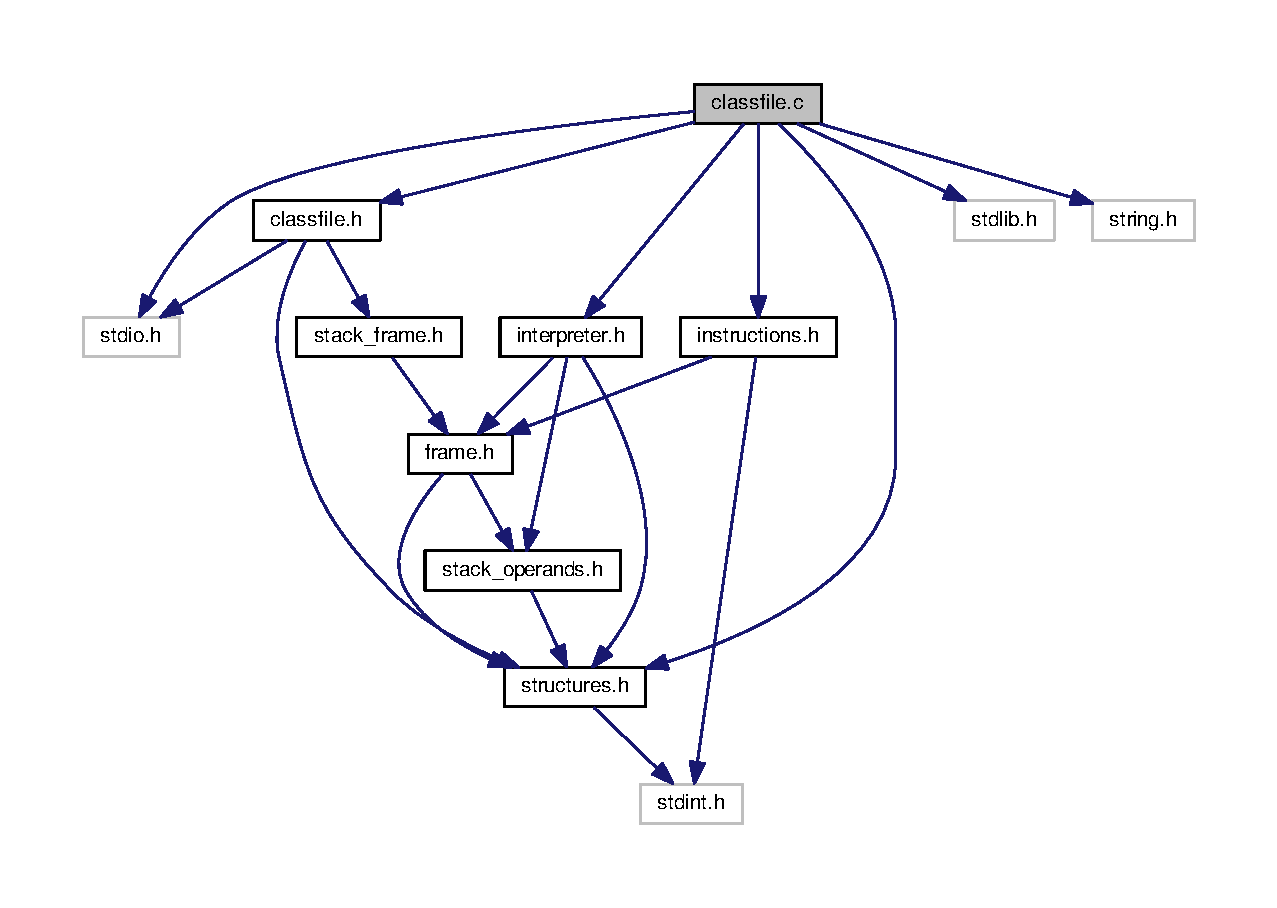
\includegraphics[width=350pt]{classfile_8c__incl}
\end{center}
\end{figure}
\subsection*{Functions}
\begin{DoxyCompactItemize}
\item 
\hyperlink{structures_8h_a64f8055b64cf2a4c299c841130c5c938}{u1} \hyperlink{classfile_8c_a13b463381f7cf580d002e6631c0c4ea8}{u1\+Read} (F\+I\+LE $\ast$file)
\begin{DoxyCompactList}\small\item\em Faz a leitura de 1 byte do arquivo .class fornecido no path. \end{DoxyCompactList}\item 
\hyperlink{structures_8h_a55ef8d87fd202b8417704c089899c5b9}{u2} \hyperlink{classfile_8c_aae51575c6f1d6ce808fbc88a3037c4ed}{u2\+Read} (F\+I\+LE $\ast$file)
\begin{DoxyCompactList}\small\item\em Faz a leitura de 2 bytes do arquivo .class fornecido no path. \end{DoxyCompactList}\item 
\hyperlink{structures_8h_ae391a1d79bb0c8cbc283f0283e3c098b}{u4} \hyperlink{classfile_8c_aad8c26a8aaff63010bb790df878f0950}{u4\+Read} (F\+I\+LE $\ast$file)
\begin{DoxyCompactList}\small\item\em Faz a leitura de 4 bytes do arquivo .class fornecido no path. \end{DoxyCompactList}\item 
char $\ast$ \hyperlink{classfile_8c_abbc0a67a74cf4718872b86f0a898575b}{print\+Version} (\hyperlink{structures_8h_a55ef8d87fd202b8417704c089899c5b9}{u2} version)
\begin{DoxyCompactList}\small\item\em Printa a versão do arquivo .class. \end{DoxyCompactList}\item 
char $\ast$ \hyperlink{classfile_8c_a77c5107c582c86dedb65853efabd9302}{read\+Utf8} (\hyperlink{structcp__info}{cp\+\_\+info} $\ast$cp, \hyperlink{structures_8h_a55ef8d87fd202b8417704c089899c5b9}{u2} index)
\begin{DoxyCompactList}\small\item\em Faz a leitua dos bytes no formato U\+T\+F-\/8. \end{DoxyCompactList}\item 
void \hyperlink{classfile_8c_aa73a2b8f66296e2fcdec5b6f029c1f88}{print\+Const\+Type} (\hyperlink{structures_8h_ae391a1d79bb0c8cbc283f0283e3c098b}{u4} high\+\_\+bytes, \hyperlink{structures_8h_ae391a1d79bb0c8cbc283f0283e3c098b}{u4} low\+\_\+bytes, \hyperlink{structures_8h_a64f8055b64cf2a4c299c841130c5c938}{u1} type)
\begin{DoxyCompactList}\small\item\em Printa o tipo C\+O\+N\+S\+T\+A\+NT. \end{DoxyCompactList}\item 
char $\ast$ \hyperlink{classfile_8c_aae8cbe5dd2db133b98988d9da5c5efe7}{print\+Type} (\hyperlink{structures_8h_a55ef8d87fd202b8417704c089899c5b9}{u2} type)
\begin{DoxyCompactList}\small\item\em Printa o tipo do objeto. \end{DoxyCompactList}\item 
char $\ast$ \hyperlink{classfile_8c_a5636f6173ac96d0316cd018b68b34034}{print\+Flag} (\hyperlink{structures_8h_a55ef8d87fd202b8417704c089899c5b9}{u2} type, \hyperlink{structures_8h_a64f8055b64cf2a4c299c841130c5c938}{u1} flag)
\begin{DoxyCompactList}\small\item\em Printa a flag correspondente ao tipo recebido. \end{DoxyCompactList}\item 
\hyperlink{structattribute__info}{attribute\+\_\+info} $\ast$ \hyperlink{classfile_8c_ab2c33d049c34b50ead32e4568387353c}{read\+Attributes} (\hyperlink{structcp__info}{cp\+\_\+info} $\ast$cp, \hyperlink{structures_8h_a55ef8d87fd202b8417704c089899c5b9}{u2} attr\+\_\+count, F\+I\+LE $\ast$fp)
\begin{DoxyCompactList}\small\item\em Lê os atributos do bytecode recebido. \end{DoxyCompactList}\item 
void \hyperlink{classfile_8c_ab694dc30480958e872cdf78b94b9cefa}{print\+Verification\+Type\+Info} (\hyperlink{structverification__type__info}{verification\+\_\+type\+\_\+info} $\ast$ver\+\_\+type, \hyperlink{structcp__info}{cp\+\_\+info} $\ast$cp, \hyperlink{structures_8h_a55ef8d87fd202b8417704c089899c5b9}{u2} verification\+\_\+type\+\_\+length)
\begin{DoxyCompactList}\small\item\em Printa o tipo a partir da tag. \end{DoxyCompactList}\item 
\hyperlink{structverification__type__info}{verification\+\_\+type\+\_\+info} $\ast$ \hyperlink{classfile_8c_add61e24daf8356973e908b3f1cfd5a24}{fill\+Verification\+Type\+Info} (F\+I\+LE $\ast$fp, \hyperlink{structures_8h_a55ef8d87fd202b8417704c089899c5b9}{u2} verification\+\_\+type\+\_\+length)
\begin{DoxyCompactList}\small\item\em Faz a leitura de 1 byre do arquivo .class fornecido no path. \end{DoxyCompactList}\item 
void \hyperlink{classfile_8c_a08affa1a8eb0fbd41df9e468f2c02321}{print\+Stack\+Map\+Table} (\hyperlink{structstack__map__frame}{stack\+\_\+map\+\_\+frame} $\ast$stack\+\_\+map, \hyperlink{structcp__info}{cp\+\_\+info} $\ast$cp, \hyperlink{structattribute__info}{attribute\+\_\+info} $\ast$attr)
\item 
\hyperlink{structstack__map__frame}{stack\+\_\+map\+\_\+frame} $\ast$ \hyperlink{classfile_8c_a1258b84eec00db8fee377fea434c49b1}{fill\+Stack\+Map\+Table} (\hyperlink{structattribute__info}{attribute\+\_\+info} $\ast$attr, F\+I\+LE $\ast$fp)
\item 
void \hyperlink{classfile_8c_ac72c096a138416b9909fe3e29417763e}{free\+Stack\+Map\+Table} (\hyperlink{structstack__map__frame}{stack\+\_\+map\+\_\+frame} $\ast$stack\+\_\+map, \hyperlink{structattribute__info}{attribute\+\_\+info} $\ast$attr)
\item 
void \hyperlink{classfile_8c_a3bfb911a1e769d93bb0e18492aab956b}{free\+Attributes} (\hyperlink{structattribute__info}{attribute\+\_\+info} $\ast$field, \hyperlink{structcp__info}{cp\+\_\+info} $\ast$cp, \hyperlink{structures_8h_a55ef8d87fd202b8417704c089899c5b9}{u2} attr\+\_\+count)
\begin{DoxyCompactList}\small\item\em Função utilizada para liberar a memória ocupada pelo classfile. \end{DoxyCompactList}\item 
void \hyperlink{classfile_8c_af82a9138759e74a734c2ba5db6077805}{print\+Attributes} (\hyperlink{structattribute__info}{attribute\+\_\+info} $\ast$field, \hyperlink{structcp__info}{cp\+\_\+info} $\ast$cp, \hyperlink{structures_8h_a55ef8d87fd202b8417704c089899c5b9}{u2} attr\+\_\+count)
\begin{DoxyCompactList}\small\item\em Printa os atributos de um classfile. \end{DoxyCompactList}\item 
void \hyperlink{classfile_8c_a8d5e46a5df7dfb965306e8a277783511}{eval\+Attributes} (\hyperlink{structattribute__info}{attribute\+\_\+info} $\ast$field, \hyperlink{structcp__info}{cp\+\_\+info} $\ast$cp, \hyperlink{structures_8h_a55ef8d87fd202b8417704c089899c5b9}{u2} attr\+\_\+count, \hyperlink{structClassFile}{Class\+File} $\ast$cf)
\begin{DoxyCompactList}\small\item\em todo\+: avalia os atributos do classfile. \end{DoxyCompactList}\item 
void \hyperlink{classfile_8c_a14c4d3f84dd03a43aca0a57bd530f3a2}{read\+\_\+class\+\_\+file} (\hyperlink{structClassFile}{Class\+File} $\ast$cf, char $\ast$file\+\_\+name)
\begin{DoxyCompactList}\small\item\em Faz a leitura do arquivo .class. \end{DoxyCompactList}\item 
void \hyperlink{classfile_8c_a774f5149d9c3dadc60b2c0ca012bf51d}{recursive\+\_\+print} (\hyperlink{structcp__info}{cp\+\_\+info} $\ast$cp, \hyperlink{structures_8h_a55ef8d87fd202b8417704c089899c5b9}{u2} index, char $\ast$str)
\begin{DoxyCompactList}\small\item\em Usa um índice para acessar a constant pool e printar recusrivamente os campos. \end{DoxyCompactList}\item 
char $\ast$ \hyperlink{classfile_8c_a580d63d9a7b152364691f69863dc7a4e}{rec\+\_\+method\+\_\+name} (\hyperlink{structcp__info}{cp\+\_\+info} $\ast$cp, \hyperlink{structures_8h_a55ef8d87fd202b8417704c089899c5b9}{u2} index)
\begin{DoxyCompactList}\small\item\em Usa um índice no constant pool para procurar o nome de um método recursivamente. \end{DoxyCompactList}\item 
char $\ast$ \hyperlink{classfile_8c_a09f80f214aa870612fcb23597bcfb4bc}{print\+\_\+reference} (\hyperlink{structcp__info}{cp\+\_\+info} $\ast$cp, \hyperlink{structures_8h_a55ef8d87fd202b8417704c089899c5b9}{u2} index)
\begin{DoxyCompactList}\small\item\em Usa um índice na constant pool para retorna uma referência no ponteiro global. \end{DoxyCompactList}\item 
char $\ast$ \hyperlink{classfile_8c_a627193785e98bc076b257c97ccd5892b}{ret\+\_\+method\+\_\+name} (\hyperlink{structcp__info}{cp\+\_\+info} $\ast$cp, \hyperlink{structures_8h_a55ef8d87fd202b8417704c089899c5b9}{u2} index)
\begin{DoxyCompactList}\small\item\em Retorna o nome de um método no ponteiro global. \end{DoxyCompactList}\item 
void \hyperlink{classfile_8c_a67e8b211dae28d036af3a55b698da993}{print\+\_\+class\+\_\+file} (\hyperlink{structClassFile}{Class\+File} $\ast$cf)
\begin{DoxyCompactList}\small\item\em Recebe um classfile como parâmetro e printa seu conteúdo de maneira organizada no terminal. (Utilizado pelo leitor/exibidor de bytecode). \end{DoxyCompactList}\item 
void \hyperlink{classfile_8c_a6a7ca9bbe1c17ec34271f8c898832ee0}{free\+\_\+class\+\_\+file} (\hyperlink{structClassFile}{Class\+File} $\ast$cf)
\begin{DoxyCompactList}\small\item\em Libera o classfile da memória. \end{DoxyCompactList}\item 
char $\ast$ \hyperlink{classfile_8c_af82954dceccc52fab4a547f79967244f}{remove\+Extension} (char $\ast$string)
\begin{DoxyCompactList}\small\item\em Remove exetensão de uma string para printar de maneira correta. \end{DoxyCompactList}\item 
char $\ast$ \hyperlink{classfile_8c_a50ab5cb2c7741908305afda2e2a0235a}{find\+Name\+File} (char $\ast$string)
\item 
void \hyperlink{classfile_8c_a55c80ae86c1c6d0666108a825df64a4b}{execute\+\_\+gvm} ()
\begin{DoxyCompactList}\small\item\em Função que busca pelo \hyperlink{structFrame}{Frame} no topo da pilha de frames e inicia a execução da \hyperlink{structJVM}{J\+VM}. Essa função é executada enquanto ainda há frames na pilha da \hyperlink{structJVM}{J\+VM}. \end{DoxyCompactList}\item 
\hyperlink{structmethod__info}{method\+\_\+info} $\ast$ \hyperlink{classfile_8c_a915037a0d75520090926e178259cf4bb}{find\+\_\+method} (\hyperlink{structClassFile}{Class\+File} $\ast$cf, char $\ast$method, char $\ast$method\+\_\+description)
\item 
\hyperlink{structures_8h_ae391a1d79bb0c8cbc283f0283e3c098b}{u4} \hyperlink{classfile_8c_abd0631a75f72632c5606e72f6d3f00ae}{Class\+Loader} (char $\ast$class\+\_\+name)
\begin{DoxyCompactList}\small\item\em Aloca espaço para o \hyperlink{structClassFile}{Class\+File} em memória e chama a função read\+\_\+class\+\_\+file para ler o \hyperlink{structClassFile}{Class\+File} recebido nas posições corretas. \end{DoxyCompactList}\item 
\hyperlink{structures_8h_a55ef8d87fd202b8417704c089899c5b9}{u2} \hyperlink{classfile_8c_a64bd697d9f3c3360d6c4edb38f8cdf60}{find\+\_\+class} (char $\ast$class\+\_\+name)
\begin{DoxyCompactList}\small\item\em Procura por cuma classe, e caso não consiga encontrá-\/la, carrega na memória usando a função Class\+Loader. \end{DoxyCompactList}\item 
\hyperlink{structfield__info}{field\+\_\+info} $\ast$ \hyperlink{classfile_8c_a0688afe113144b86408f83f83685db04}{find\+\_\+field} (\hyperlink{structClassFile}{Class\+File} $\ast$cf, char $\ast$field\+\_\+name, char $\ast$field\+\_\+desc)
\begin{DoxyCompactList}\small\item\em Procura por um field dentro do \hyperlink{structClassFile}{Class\+File}. \end{DoxyCompactList}\item 
void \hyperlink{classfile_8c_a39063f00cc6ccce0402e1a81f2f760af}{find\+\_\+clinit} (\hyperlink{structClassFile}{Class\+File} $\ast$cf)
\begin{DoxyCompactList}\small\item\em Procura por um init dentro do Classfile. \end{DoxyCompactList}\end{DoxyCompactItemize}


\subsection{Detailed Description}
Classfile functions  Funções de apoio e leitura do \hyperlink{structClassFile}{Class\+File} (bytecode) 



\subsection{Function Documentation}
\index{classfile.\+c@{classfile.\+c}!Class\+Loader@{Class\+Loader}}
\index{Class\+Loader@{Class\+Loader}!classfile.\+c@{classfile.\+c}}
\subsubsection[{\texorpdfstring{Class\+Loader(char $\ast$class\+\_\+name)}{ClassLoader(char *class_name)}}]{\setlength{\rightskip}{0pt plus 5cm}{\bf u4} Class\+Loader (
\begin{DoxyParamCaption}
\item[{char $\ast$}]{class\+\_\+name}
\end{DoxyParamCaption}
)}\hypertarget{classfile_8c_abd0631a75f72632c5606e72f6d3f00ae}{}\label{classfile_8c_abd0631a75f72632c5606e72f6d3f00ae}


Aloca espaço para o \hyperlink{structClassFile}{Class\+File} em memória e chama a função read\+\_\+class\+\_\+file para ler o \hyperlink{structClassFile}{Class\+File} recebido nas posições corretas. 



Here is the call graph for this function\+:
\nopagebreak
\begin{figure}[H]
\begin{center}
\leavevmode
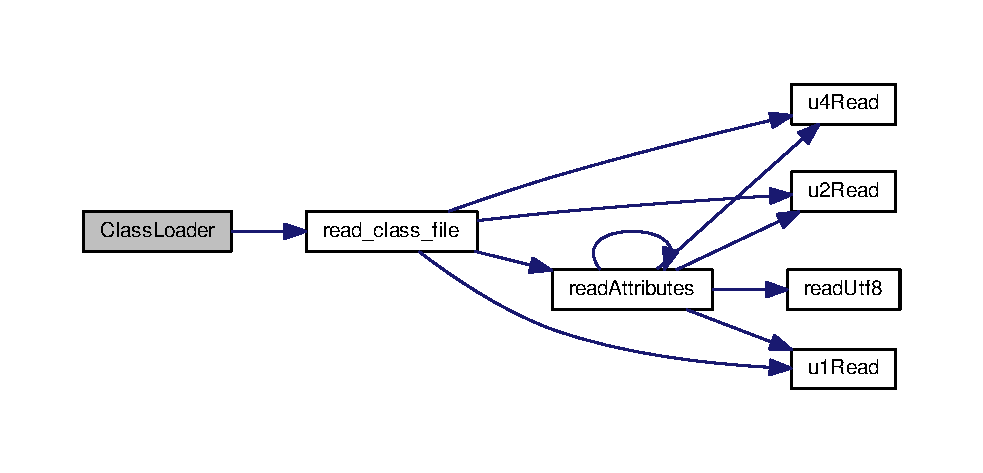
\includegraphics[width=350pt]{classfile_8c_abd0631a75f72632c5606e72f6d3f00ae_cgraph}
\end{center}
\end{figure}




Here is the caller graph for this function\+:
\nopagebreak
\begin{figure}[H]
\begin{center}
\leavevmode
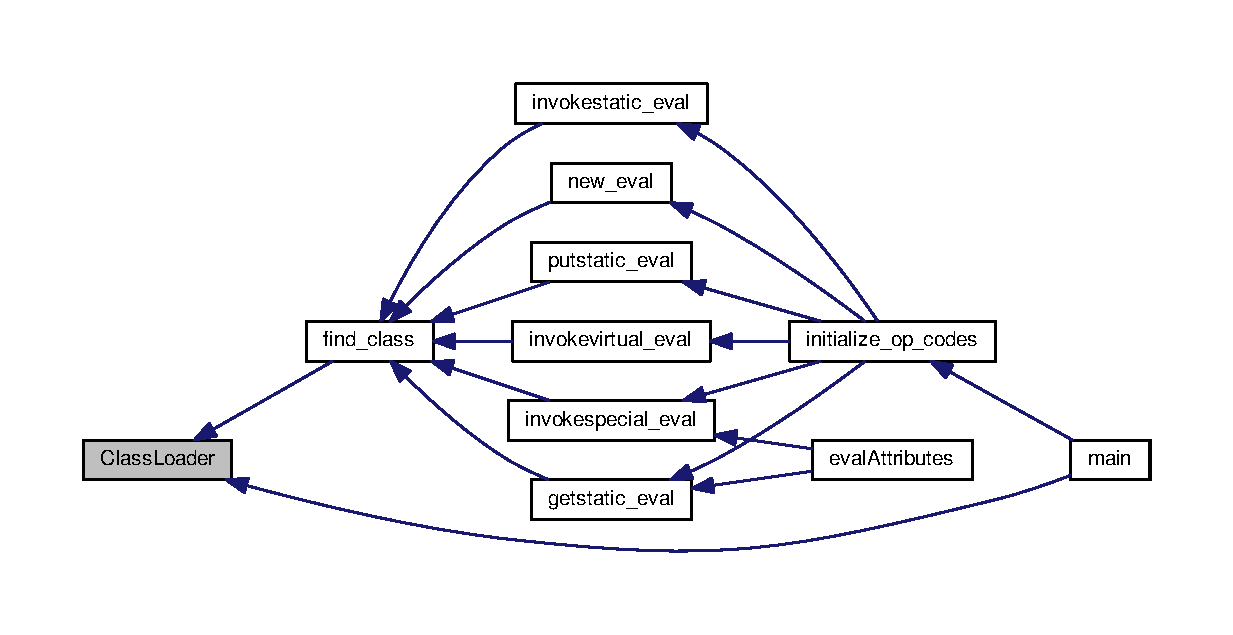
\includegraphics[width=350pt]{classfile_8c_abd0631a75f72632c5606e72f6d3f00ae_icgraph}
\end{center}
\end{figure}


\index{classfile.\+c@{classfile.\+c}!eval\+Attributes@{eval\+Attributes}}
\index{eval\+Attributes@{eval\+Attributes}!classfile.\+c@{classfile.\+c}}
\subsubsection[{\texorpdfstring{eval\+Attributes(attribute\+\_\+info $\ast$field, cp\+\_\+info $\ast$cp, u2 attr\+\_\+count, Class\+File $\ast$cf)}{evalAttributes(attribute_info *field, cp_info *cp, u2 attr_count, ClassFile *cf)}}]{\setlength{\rightskip}{0pt plus 5cm}void eval\+Attributes (
\begin{DoxyParamCaption}
\item[{{\bf attribute\+\_\+info} $\ast$}]{field, }
\item[{{\bf cp\+\_\+info} $\ast$}]{cp, }
\item[{{\bf u2}}]{attr\+\_\+count, }
\item[{{\bf Class\+File} $\ast$}]{cf}
\end{DoxyParamCaption}
)}\hypertarget{classfile_8c_a8d5e46a5df7dfb965306e8a277783511}{}\label{classfile_8c_a8d5e46a5df7dfb965306e8a277783511}


todo\+: avalia os atributos do classfile. 



Here is the call graph for this function\+:
\nopagebreak
\begin{figure}[H]
\begin{center}
\leavevmode
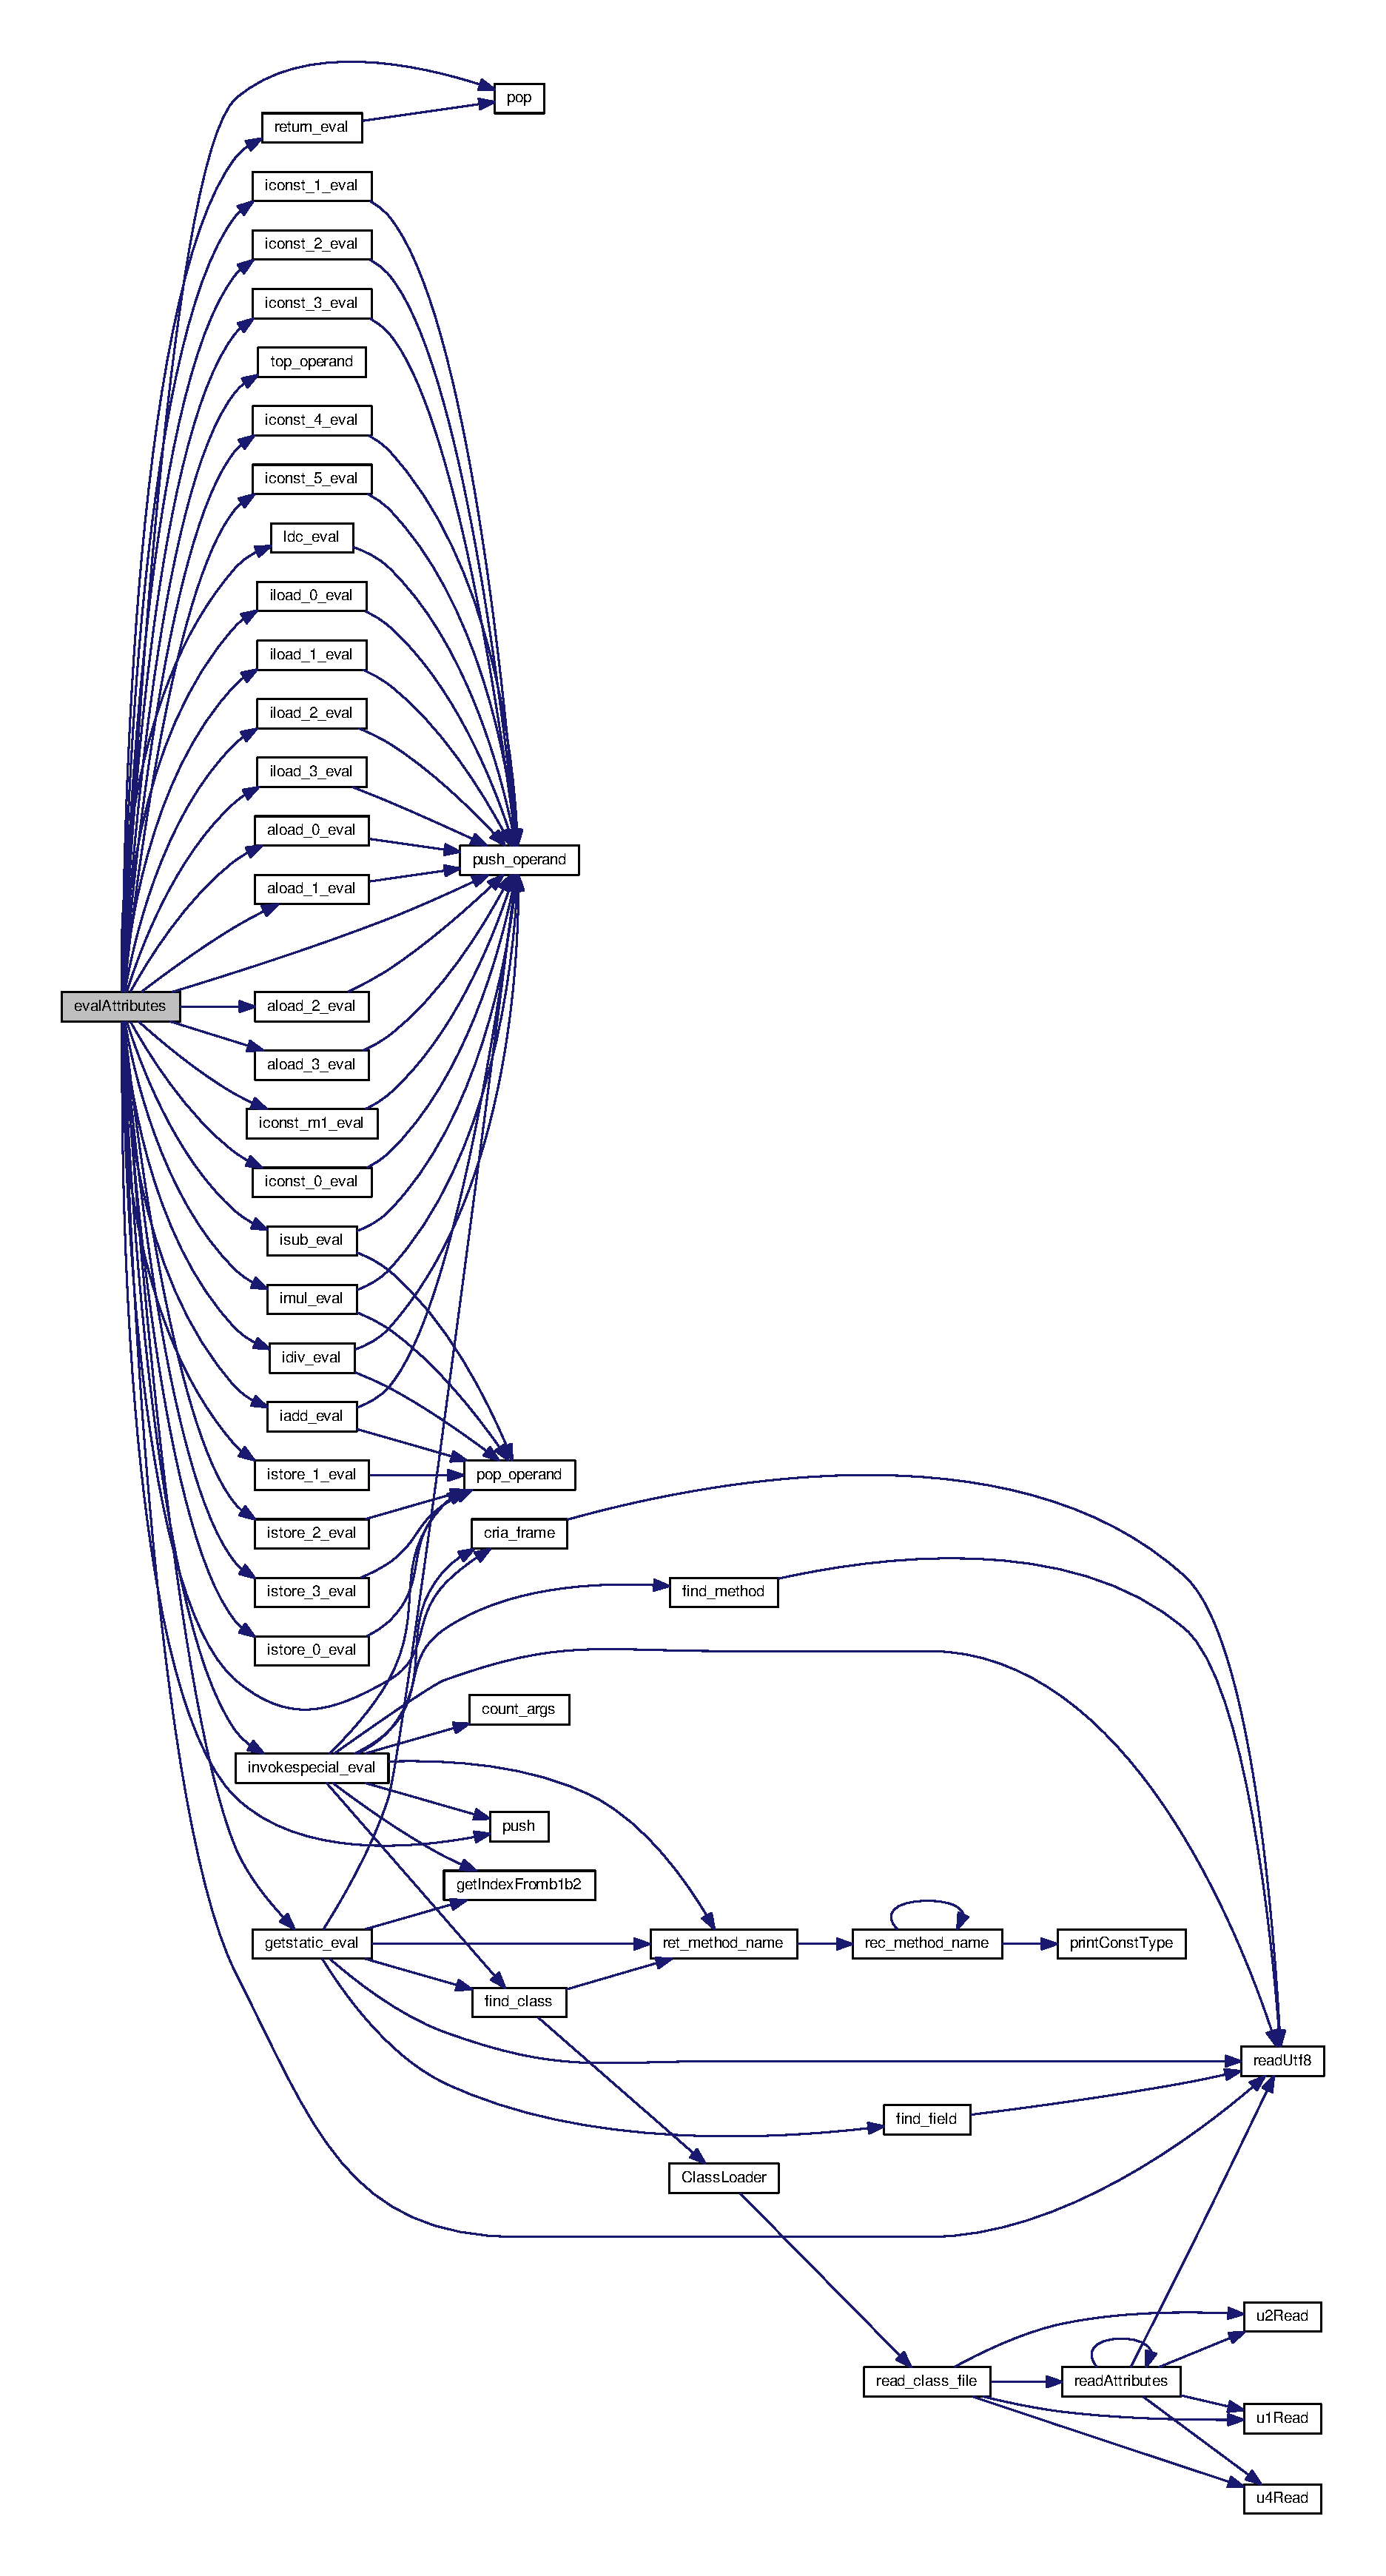
\includegraphics[height=550pt]{classfile_8c_a8d5e46a5df7dfb965306e8a277783511_cgraph}
\end{center}
\end{figure}


\index{classfile.\+c@{classfile.\+c}!execute\+\_\+gvm@{execute\+\_\+gvm}}
\index{execute\+\_\+gvm@{execute\+\_\+gvm}!classfile.\+c@{classfile.\+c}}
\subsubsection[{\texorpdfstring{execute\+\_\+gvm()}{execute_gvm()}}]{\setlength{\rightskip}{0pt plus 5cm}void execute\+\_\+gvm (
\begin{DoxyParamCaption}
{}
\end{DoxyParamCaption}
)}\hypertarget{classfile_8c_a55c80ae86c1c6d0666108a825df64a4b}{}\label{classfile_8c_a55c80ae86c1c6d0666108a825df64a4b}


Função que busca pelo \hyperlink{structFrame}{Frame} no topo da pilha de frames e inicia a execução da \hyperlink{structJVM}{J\+VM}. Essa função é executada enquanto ainda há frames na pilha da \hyperlink{structJVM}{J\+VM}. 



Here is the call graph for this function\+:
\nopagebreak
\begin{figure}[H]
\begin{center}
\leavevmode
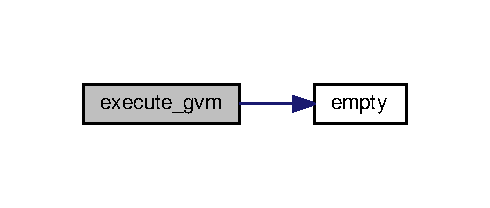
\includegraphics[width=235pt]{classfile_8c_a55c80ae86c1c6d0666108a825df64a4b_cgraph}
\end{center}
\end{figure}




Here is the caller graph for this function\+:
\nopagebreak
\begin{figure}[H]
\begin{center}
\leavevmode
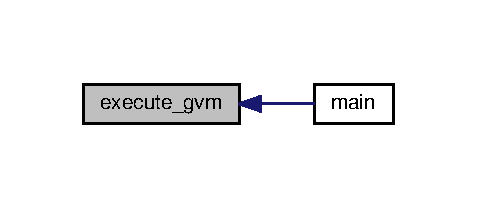
\includegraphics[width=229pt]{classfile_8c_a55c80ae86c1c6d0666108a825df64a4b_icgraph}
\end{center}
\end{figure}


\index{classfile.\+c@{classfile.\+c}!fill\+Stack\+Map\+Table@{fill\+Stack\+Map\+Table}}
\index{fill\+Stack\+Map\+Table@{fill\+Stack\+Map\+Table}!classfile.\+c@{classfile.\+c}}
\subsubsection[{\texorpdfstring{fill\+Stack\+Map\+Table(attribute\+\_\+info $\ast$attr, F\+I\+L\+E $\ast$fp)}{fillStackMapTable(attribute_info *attr, FILE *fp)}}]{\setlength{\rightskip}{0pt plus 5cm}{\bf stack\+\_\+map\+\_\+frame}$\ast$ fill\+Stack\+Map\+Table (
\begin{DoxyParamCaption}
\item[{{\bf attribute\+\_\+info} $\ast$}]{attr, }
\item[{F\+I\+LE $\ast$}]{fp}
\end{DoxyParamCaption}
)}\hypertarget{classfile_8c_a1258b84eec00db8fee377fea434c49b1}{}\label{classfile_8c_a1258b84eec00db8fee377fea434c49b1}


Here is the call graph for this function\+:
\nopagebreak
\begin{figure}[H]
\begin{center}
\leavevmode
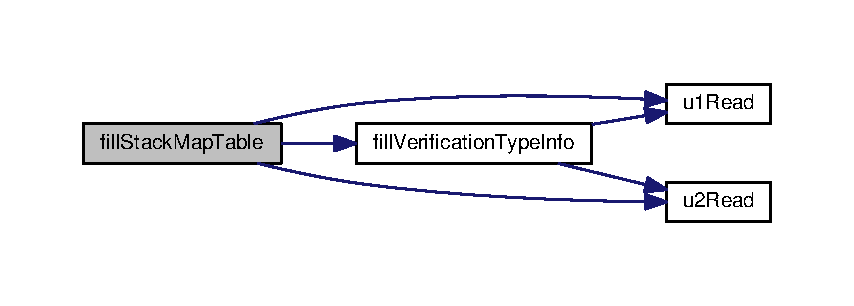
\includegraphics[width=350pt]{classfile_8c_a1258b84eec00db8fee377fea434c49b1_cgraph}
\end{center}
\end{figure}


\index{classfile.\+c@{classfile.\+c}!fill\+Verification\+Type\+Info@{fill\+Verification\+Type\+Info}}
\index{fill\+Verification\+Type\+Info@{fill\+Verification\+Type\+Info}!classfile.\+c@{classfile.\+c}}
\subsubsection[{\texorpdfstring{fill\+Verification\+Type\+Info(\+F\+I\+L\+E $\ast$fp, u2 verification\+\_\+type\+\_\+length)}{fillVerificationTypeInfo(FILE *fp, u2 verification_type_length)}}]{\setlength{\rightskip}{0pt plus 5cm}{\bf verification\+\_\+type\+\_\+info}$\ast$ fill\+Verification\+Type\+Info (
\begin{DoxyParamCaption}
\item[{F\+I\+LE $\ast$}]{fp, }
\item[{{\bf u2}}]{verification\+\_\+type\+\_\+length}
\end{DoxyParamCaption}
)}\hypertarget{classfile_8c_add61e24daf8356973e908b3f1cfd5a24}{}\label{classfile_8c_add61e24daf8356973e908b3f1cfd5a24}


Faz a leitura de 1 byre do arquivo .class fornecido no path. 



Here is the call graph for this function\+:
\nopagebreak
\begin{figure}[H]
\begin{center}
\leavevmode
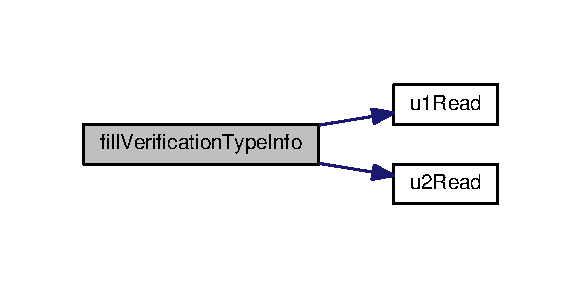
\includegraphics[width=279pt]{classfile_8c_add61e24daf8356973e908b3f1cfd5a24_cgraph}
\end{center}
\end{figure}




Here is the caller graph for this function\+:
\nopagebreak
\begin{figure}[H]
\begin{center}
\leavevmode
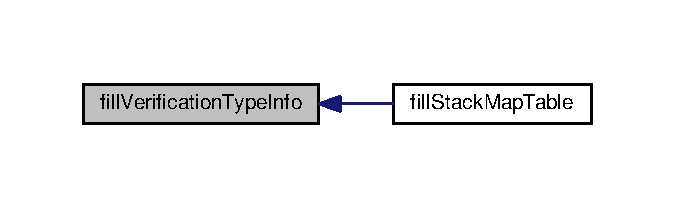
\includegraphics[width=324pt]{classfile_8c_add61e24daf8356973e908b3f1cfd5a24_icgraph}
\end{center}
\end{figure}


\index{classfile.\+c@{classfile.\+c}!find\+\_\+class@{find\+\_\+class}}
\index{find\+\_\+class@{find\+\_\+class}!classfile.\+c@{classfile.\+c}}
\subsubsection[{\texorpdfstring{find\+\_\+class(char $\ast$class\+\_\+name)}{find_class(char *class_name)}}]{\setlength{\rightskip}{0pt plus 5cm}{\bf u2} find\+\_\+class (
\begin{DoxyParamCaption}
\item[{char $\ast$}]{class\+\_\+name}
\end{DoxyParamCaption}
)}\hypertarget{classfile_8c_a64bd697d9f3c3360d6c4edb38f8cdf60}{}\label{classfile_8c_a64bd697d9f3c3360d6c4edb38f8cdf60}


Procura por cuma classe, e caso não consiga encontrá-\/la, carrega na memória usando a função Class\+Loader. 



Here is the call graph for this function\+:
\nopagebreak
\begin{figure}[H]
\begin{center}
\leavevmode
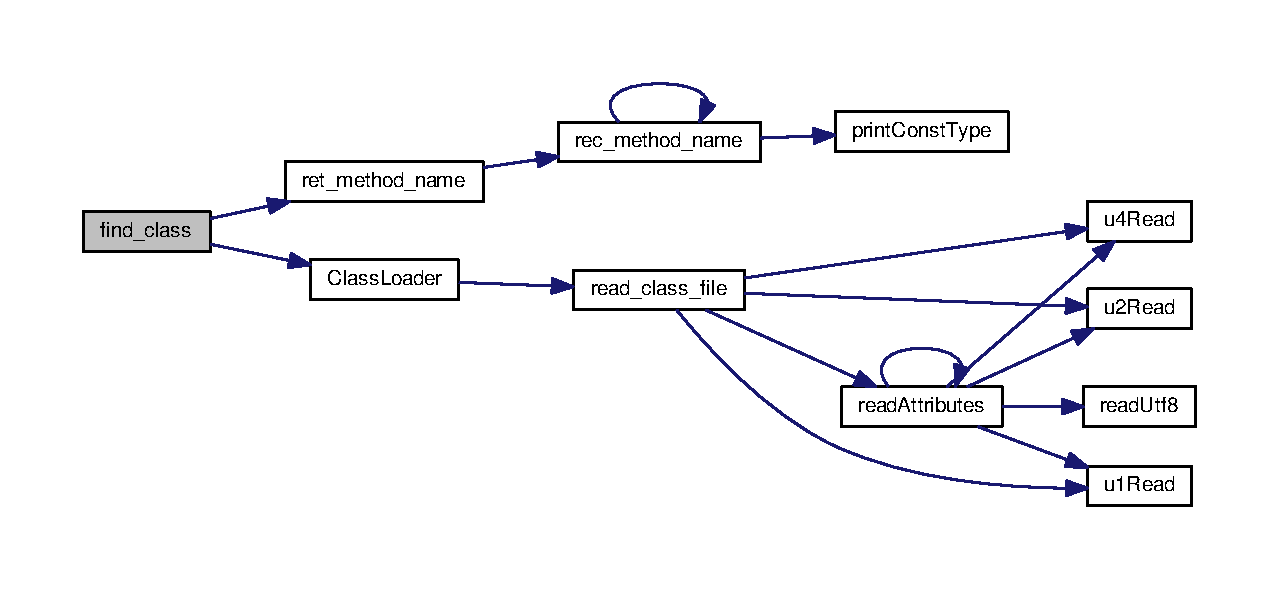
\includegraphics[width=350pt]{classfile_8c_a64bd697d9f3c3360d6c4edb38f8cdf60_cgraph}
\end{center}
\end{figure}




Here is the caller graph for this function\+:
\nopagebreak
\begin{figure}[H]
\begin{center}
\leavevmode
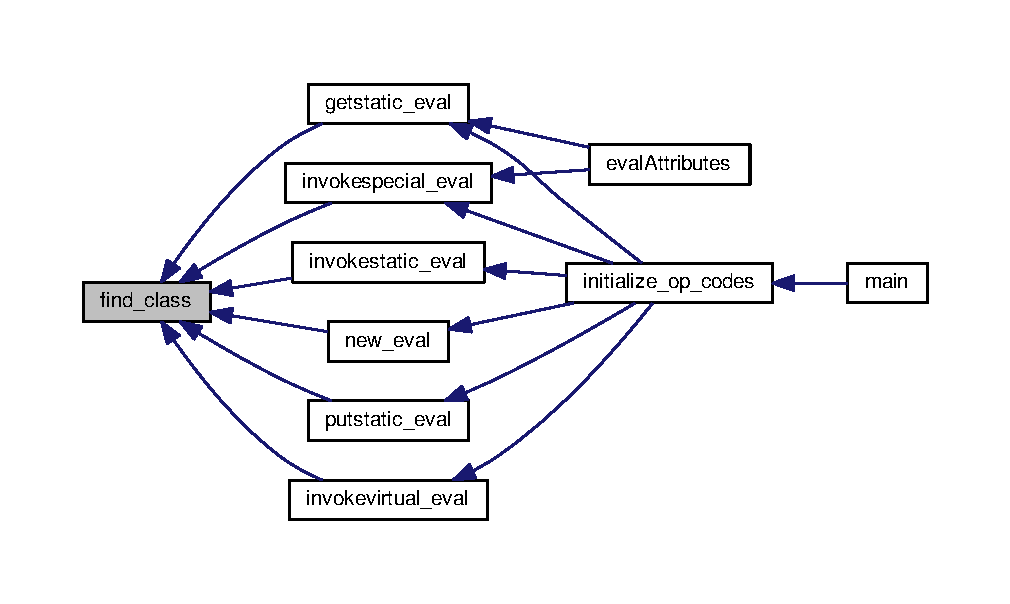
\includegraphics[width=350pt]{classfile_8c_a64bd697d9f3c3360d6c4edb38f8cdf60_icgraph}
\end{center}
\end{figure}


\index{classfile.\+c@{classfile.\+c}!find\+\_\+clinit@{find\+\_\+clinit}}
\index{find\+\_\+clinit@{find\+\_\+clinit}!classfile.\+c@{classfile.\+c}}
\subsubsection[{\texorpdfstring{find\+\_\+clinit(\+Class\+File $\ast$cf)}{find_clinit(ClassFile *cf)}}]{\setlength{\rightskip}{0pt plus 5cm}void find\+\_\+clinit (
\begin{DoxyParamCaption}
\item[{{\bf Class\+File} $\ast$}]{cf}
\end{DoxyParamCaption}
)}\hypertarget{classfile_8c_a39063f00cc6ccce0402e1a81f2f760af}{}\label{classfile_8c_a39063f00cc6ccce0402e1a81f2f760af}


Procura por um init dentro do Classfile. 



Here is the call graph for this function\+:
\nopagebreak
\begin{figure}[H]
\begin{center}
\leavevmode
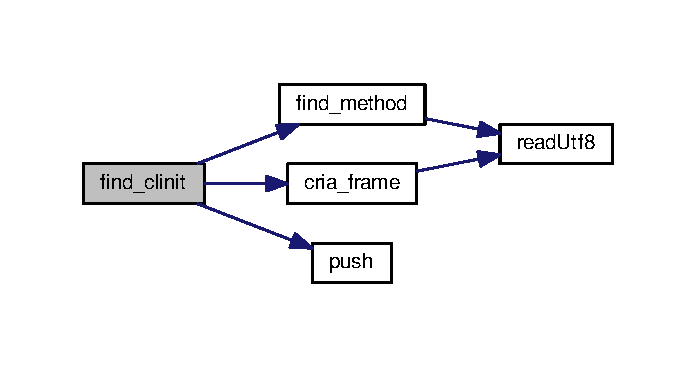
\includegraphics[width=334pt]{classfile_8c_a39063f00cc6ccce0402e1a81f2f760af_cgraph}
\end{center}
\end{figure}




Here is the caller graph for this function\+:
\nopagebreak
\begin{figure}[H]
\begin{center}
\leavevmode
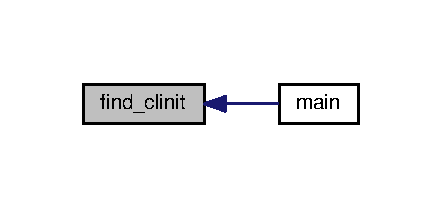
\includegraphics[width=212pt]{classfile_8c_a39063f00cc6ccce0402e1a81f2f760af_icgraph}
\end{center}
\end{figure}


\index{classfile.\+c@{classfile.\+c}!find\+\_\+field@{find\+\_\+field}}
\index{find\+\_\+field@{find\+\_\+field}!classfile.\+c@{classfile.\+c}}
\subsubsection[{\texorpdfstring{find\+\_\+field(\+Class\+File $\ast$cf, char $\ast$field\+\_\+name, char $\ast$field\+\_\+desc)}{find_field(ClassFile *cf, char *field_name, char *field_desc)}}]{\setlength{\rightskip}{0pt plus 5cm}{\bf field\+\_\+info}$\ast$ find\+\_\+field (
\begin{DoxyParamCaption}
\item[{{\bf Class\+File} $\ast$}]{cf, }
\item[{char $\ast$}]{field\+\_\+name, }
\item[{char $\ast$}]{field\+\_\+desc}
\end{DoxyParamCaption}
)}\hypertarget{classfile_8c_a0688afe113144b86408f83f83685db04}{}\label{classfile_8c_a0688afe113144b86408f83f83685db04}


Procura por um field dentro do \hyperlink{structClassFile}{Class\+File}. 



Here is the call graph for this function\+:
\nopagebreak
\begin{figure}[H]
\begin{center}
\leavevmode
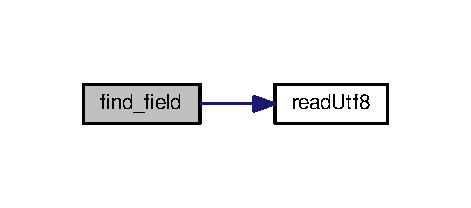
\includegraphics[width=226pt]{classfile_8c_a0688afe113144b86408f83f83685db04_cgraph}
\end{center}
\end{figure}




Here is the caller graph for this function\+:
\nopagebreak
\begin{figure}[H]
\begin{center}
\leavevmode
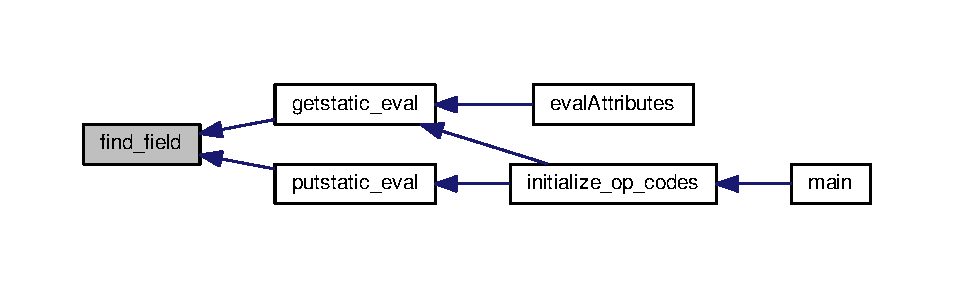
\includegraphics[width=350pt]{classfile_8c_a0688afe113144b86408f83f83685db04_icgraph}
\end{center}
\end{figure}


\index{classfile.\+c@{classfile.\+c}!find\+\_\+method@{find\+\_\+method}}
\index{find\+\_\+method@{find\+\_\+method}!classfile.\+c@{classfile.\+c}}
\subsubsection[{\texorpdfstring{find\+\_\+method(\+Class\+File $\ast$cf, char $\ast$method, char $\ast$method\+\_\+description)}{find_method(ClassFile *cf, char *method, char *method_description)}}]{\setlength{\rightskip}{0pt plus 5cm}{\bf method\+\_\+info}$\ast$ find\+\_\+method (
\begin{DoxyParamCaption}
\item[{{\bf Class\+File} $\ast$}]{cf, }
\item[{char $\ast$}]{method, }
\item[{char $\ast$}]{method\+\_\+description}
\end{DoxyParamCaption}
)}\hypertarget{classfile_8c_a915037a0d75520090926e178259cf4bb}{}\label{classfile_8c_a915037a0d75520090926e178259cf4bb}


Here is the call graph for this function\+:
\nopagebreak
\begin{figure}[H]
\begin{center}
\leavevmode
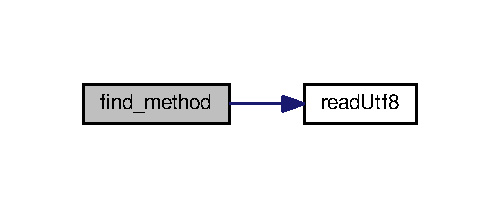
\includegraphics[width=240pt]{classfile_8c_a915037a0d75520090926e178259cf4bb_cgraph}
\end{center}
\end{figure}




Here is the caller graph for this function\+:
\nopagebreak
\begin{figure}[H]
\begin{center}
\leavevmode
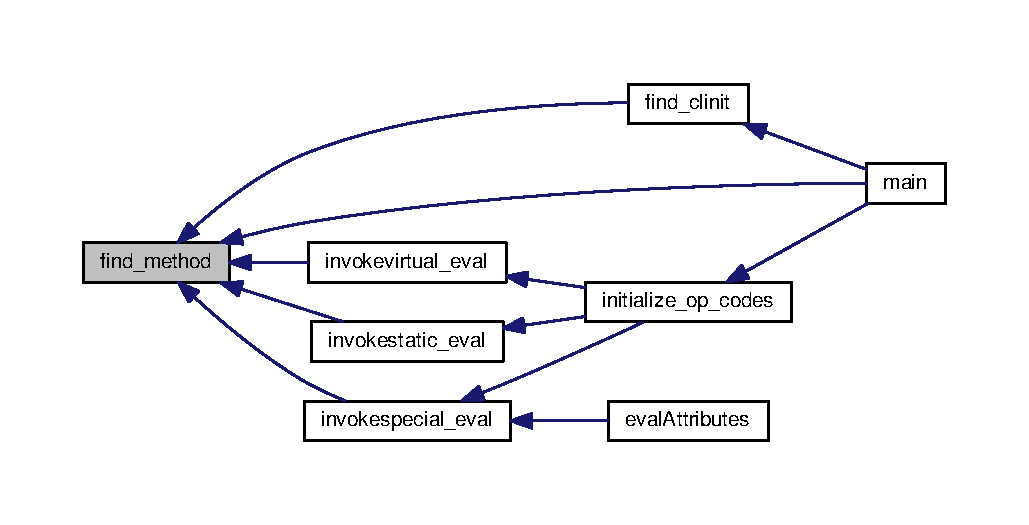
\includegraphics[width=350pt]{classfile_8c_a915037a0d75520090926e178259cf4bb_icgraph}
\end{center}
\end{figure}


\index{classfile.\+c@{classfile.\+c}!find\+Name\+File@{find\+Name\+File}}
\index{find\+Name\+File@{find\+Name\+File}!classfile.\+c@{classfile.\+c}}
\subsubsection[{\texorpdfstring{find\+Name\+File(char $\ast$string)}{findNameFile(char *string)}}]{\setlength{\rightskip}{0pt plus 5cm}char$\ast$ find\+Name\+File (
\begin{DoxyParamCaption}
\item[{char $\ast$}]{string}
\end{DoxyParamCaption}
)}\hypertarget{classfile_8c_a50ab5cb2c7741908305afda2e2a0235a}{}\label{classfile_8c_a50ab5cb2c7741908305afda2e2a0235a}


Here is the caller graph for this function\+:
\nopagebreak
\begin{figure}[H]
\begin{center}
\leavevmode
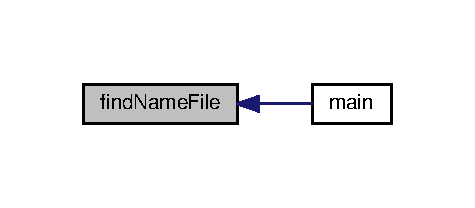
\includegraphics[width=228pt]{classfile_8c_a50ab5cb2c7741908305afda2e2a0235a_icgraph}
\end{center}
\end{figure}


\index{classfile.\+c@{classfile.\+c}!free\+\_\+class\+\_\+file@{free\+\_\+class\+\_\+file}}
\index{free\+\_\+class\+\_\+file@{free\+\_\+class\+\_\+file}!classfile.\+c@{classfile.\+c}}
\subsubsection[{\texorpdfstring{free\+\_\+class\+\_\+file(\+Class\+File $\ast$cf)}{free_class_file(ClassFile *cf)}}]{\setlength{\rightskip}{0pt plus 5cm}void free\+\_\+class\+\_\+file (
\begin{DoxyParamCaption}
\item[{{\bf Class\+File} $\ast$}]{cf}
\end{DoxyParamCaption}
)}\hypertarget{classfile_8c_a6a7ca9bbe1c17ec34271f8c898832ee0}{}\label{classfile_8c_a6a7ca9bbe1c17ec34271f8c898832ee0}


Libera o classfile da memória. 



Here is the call graph for this function\+:
\nopagebreak
\begin{figure}[H]
\begin{center}
\leavevmode
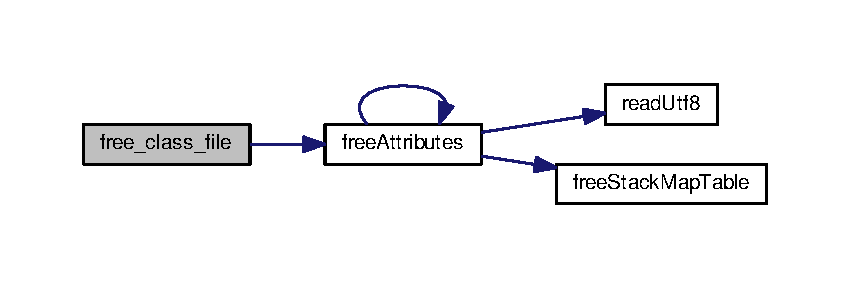
\includegraphics[width=350pt]{classfile_8c_a6a7ca9bbe1c17ec34271f8c898832ee0_cgraph}
\end{center}
\end{figure}




Here is the caller graph for this function\+:
\nopagebreak
\begin{figure}[H]
\begin{center}
\leavevmode
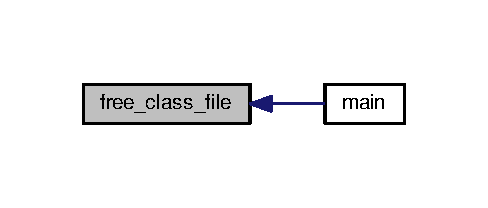
\includegraphics[width=234pt]{classfile_8c_a6a7ca9bbe1c17ec34271f8c898832ee0_icgraph}
\end{center}
\end{figure}


\index{classfile.\+c@{classfile.\+c}!free\+Attributes@{free\+Attributes}}
\index{free\+Attributes@{free\+Attributes}!classfile.\+c@{classfile.\+c}}
\subsubsection[{\texorpdfstring{free\+Attributes(attribute\+\_\+info $\ast$field, cp\+\_\+info $\ast$cp, u2 attr\+\_\+count)}{freeAttributes(attribute_info *field, cp_info *cp, u2 attr_count)}}]{\setlength{\rightskip}{0pt plus 5cm}void free\+Attributes (
\begin{DoxyParamCaption}
\item[{{\bf attribute\+\_\+info} $\ast$}]{field, }
\item[{{\bf cp\+\_\+info} $\ast$}]{cp, }
\item[{{\bf u2}}]{attr\+\_\+count}
\end{DoxyParamCaption}
)}\hypertarget{classfile_8c_a3bfb911a1e769d93bb0e18492aab956b}{}\label{classfile_8c_a3bfb911a1e769d93bb0e18492aab956b}


Função utilizada para liberar a memória ocupada pelo classfile. 



Here is the call graph for this function\+:
\nopagebreak
\begin{figure}[H]
\begin{center}
\leavevmode
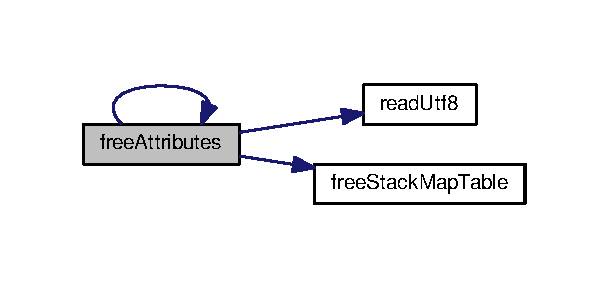
\includegraphics[width=292pt]{classfile_8c_a3bfb911a1e769d93bb0e18492aab956b_cgraph}
\end{center}
\end{figure}




Here is the caller graph for this function\+:
\nopagebreak
\begin{figure}[H]
\begin{center}
\leavevmode
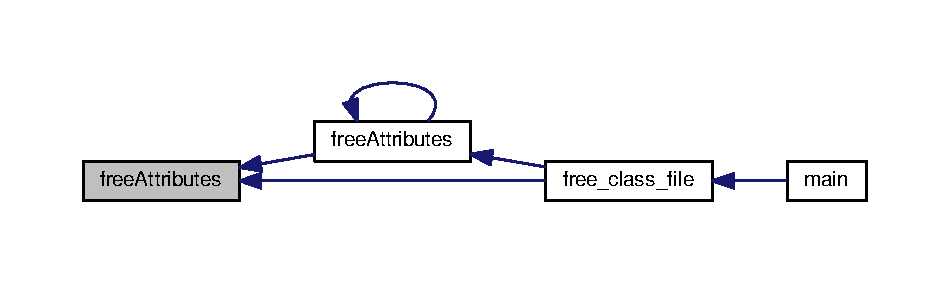
\includegraphics[width=350pt]{classfile_8c_a3bfb911a1e769d93bb0e18492aab956b_icgraph}
\end{center}
\end{figure}


\index{classfile.\+c@{classfile.\+c}!free\+Stack\+Map\+Table@{free\+Stack\+Map\+Table}}
\index{free\+Stack\+Map\+Table@{free\+Stack\+Map\+Table}!classfile.\+c@{classfile.\+c}}
\subsubsection[{\texorpdfstring{free\+Stack\+Map\+Table(stack\+\_\+map\+\_\+frame $\ast$stack\+\_\+map, attribute\+\_\+info $\ast$attr)}{freeStackMapTable(stack_map_frame *stack_map, attribute_info *attr)}}]{\setlength{\rightskip}{0pt plus 5cm}void free\+Stack\+Map\+Table (
\begin{DoxyParamCaption}
\item[{{\bf stack\+\_\+map\+\_\+frame} $\ast$}]{stack\+\_\+map, }
\item[{{\bf attribute\+\_\+info} $\ast$}]{attr}
\end{DoxyParamCaption}
)}\hypertarget{classfile_8c_ac72c096a138416b9909fe3e29417763e}{}\label{classfile_8c_ac72c096a138416b9909fe3e29417763e}


Here is the caller graph for this function\+:
\nopagebreak
\begin{figure}[H]
\begin{center}
\leavevmode
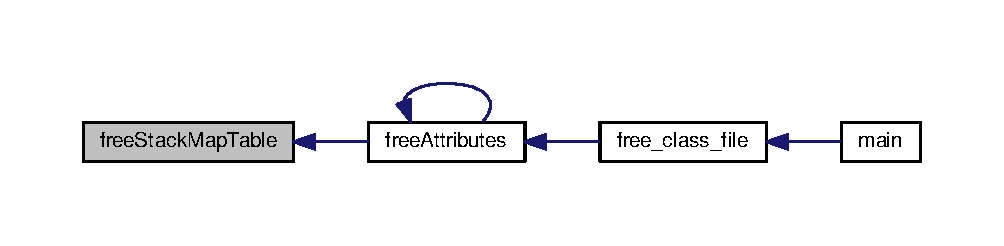
\includegraphics[width=350pt]{classfile_8c_ac72c096a138416b9909fe3e29417763e_icgraph}
\end{center}
\end{figure}


\index{classfile.\+c@{classfile.\+c}!print\+\_\+class\+\_\+file@{print\+\_\+class\+\_\+file}}
\index{print\+\_\+class\+\_\+file@{print\+\_\+class\+\_\+file}!classfile.\+c@{classfile.\+c}}
\subsubsection[{\texorpdfstring{print\+\_\+class\+\_\+file(\+Class\+File $\ast$cf)}{print_class_file(ClassFile *cf)}}]{\setlength{\rightskip}{0pt plus 5cm}void print\+\_\+class\+\_\+file (
\begin{DoxyParamCaption}
\item[{{\bf Class\+File} $\ast$}]{cf}
\end{DoxyParamCaption}
)}\hypertarget{classfile_8c_a67e8b211dae28d036af3a55b698da993}{}\label{classfile_8c_a67e8b211dae28d036af3a55b698da993}


Recebe um classfile como parâmetro e printa seu conteúdo de maneira organizada no terminal. (Utilizado pelo leitor/exibidor de bytecode). 



Here is the call graph for this function\+:
\nopagebreak
\begin{figure}[H]
\begin{center}
\leavevmode
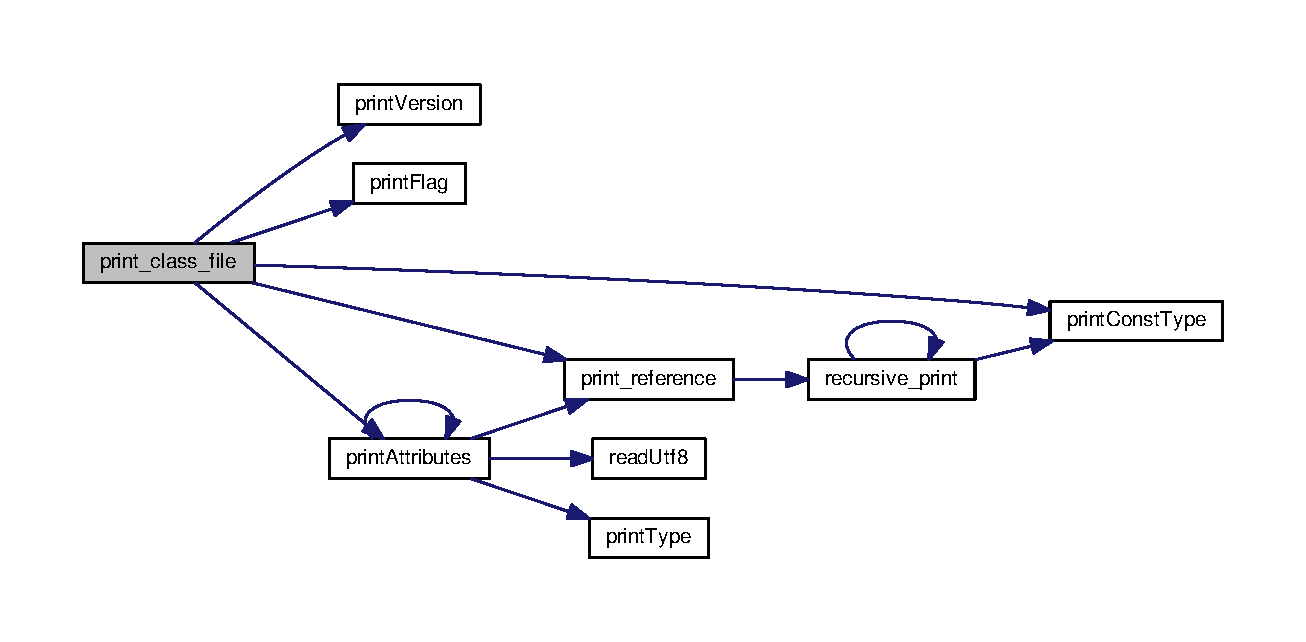
\includegraphics[width=350pt]{classfile_8c_a67e8b211dae28d036af3a55b698da993_cgraph}
\end{center}
\end{figure}




Here is the caller graph for this function\+:
\nopagebreak
\begin{figure}[H]
\begin{center}
\leavevmode
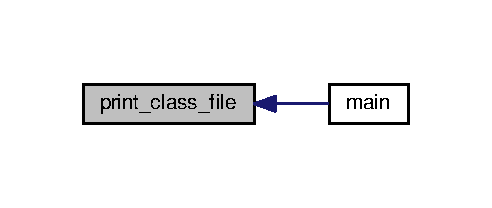
\includegraphics[width=236pt]{classfile_8c_a67e8b211dae28d036af3a55b698da993_icgraph}
\end{center}
\end{figure}


\index{classfile.\+c@{classfile.\+c}!print\+\_\+reference@{print\+\_\+reference}}
\index{print\+\_\+reference@{print\+\_\+reference}!classfile.\+c@{classfile.\+c}}
\subsubsection[{\texorpdfstring{print\+\_\+reference(cp\+\_\+info $\ast$cp, u2 index)}{print_reference(cp_info *cp, u2 index)}}]{\setlength{\rightskip}{0pt plus 5cm}char$\ast$ print\+\_\+reference (
\begin{DoxyParamCaption}
\item[{{\bf cp\+\_\+info} $\ast$}]{cp, }
\item[{{\bf u2}}]{index}
\end{DoxyParamCaption}
)}\hypertarget{classfile_8c_a09f80f214aa870612fcb23597bcfb4bc}{}\label{classfile_8c_a09f80f214aa870612fcb23597bcfb4bc}


Usa um índice na constant pool para retorna uma referência no ponteiro global. 



Here is the call graph for this function\+:
\nopagebreak
\begin{figure}[H]
\begin{center}
\leavevmode
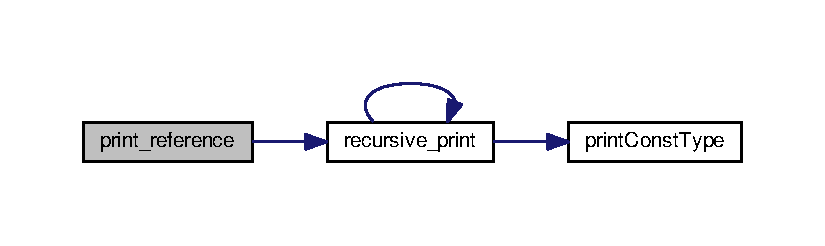
\includegraphics[width=350pt]{classfile_8c_a09f80f214aa870612fcb23597bcfb4bc_cgraph}
\end{center}
\end{figure}




Here is the caller graph for this function\+:
\nopagebreak
\begin{figure}[H]
\begin{center}
\leavevmode
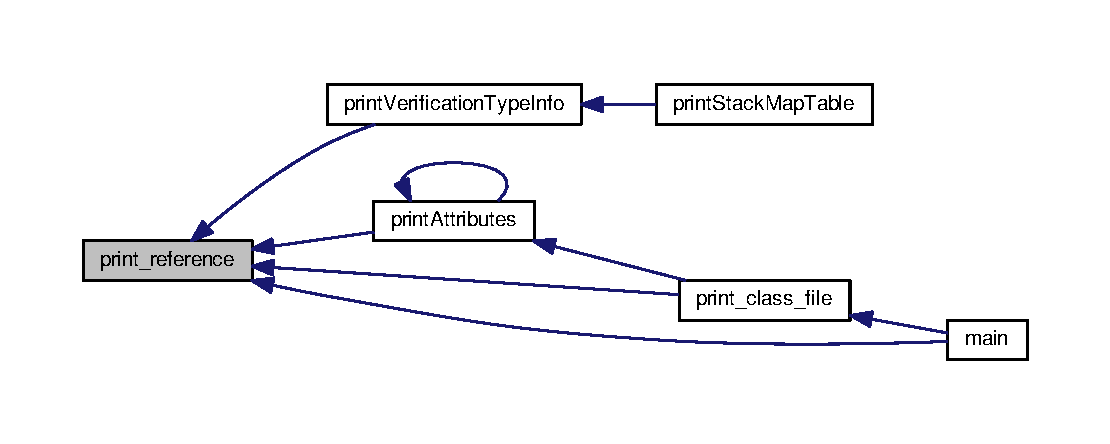
\includegraphics[width=350pt]{classfile_8c_a09f80f214aa870612fcb23597bcfb4bc_icgraph}
\end{center}
\end{figure}


\index{classfile.\+c@{classfile.\+c}!print\+Attributes@{print\+Attributes}}
\index{print\+Attributes@{print\+Attributes}!classfile.\+c@{classfile.\+c}}
\subsubsection[{\texorpdfstring{print\+Attributes(attribute\+\_\+info $\ast$field, cp\+\_\+info $\ast$cp, u2 attr\+\_\+count)}{printAttributes(attribute_info *field, cp_info *cp, u2 attr_count)}}]{\setlength{\rightskip}{0pt plus 5cm}void print\+Attributes (
\begin{DoxyParamCaption}
\item[{{\bf attribute\+\_\+info} $\ast$}]{field, }
\item[{{\bf cp\+\_\+info} $\ast$}]{cp, }
\item[{{\bf u2}}]{attr\+\_\+count}
\end{DoxyParamCaption}
)}\hypertarget{classfile_8c_af82a9138759e74a734c2ba5db6077805}{}\label{classfile_8c_af82a9138759e74a734c2ba5db6077805}


Printa os atributos de um classfile. 



Here is the call graph for this function\+:
\nopagebreak
\begin{figure}[H]
\begin{center}
\leavevmode
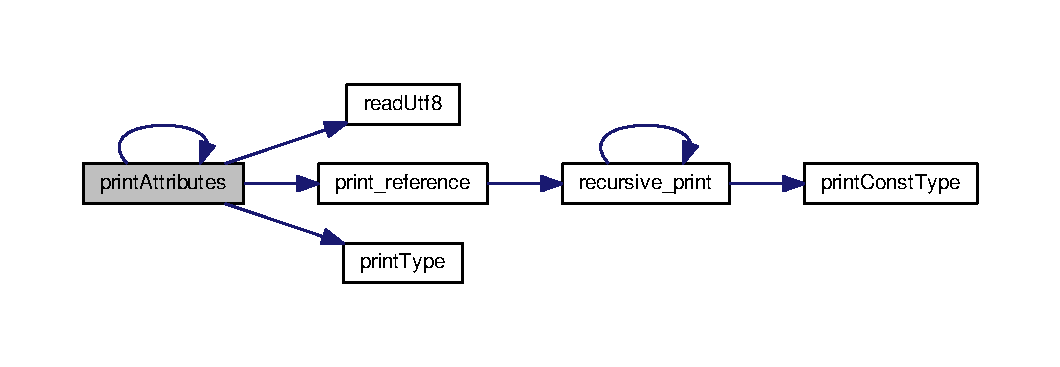
\includegraphics[width=350pt]{classfile_8c_af82a9138759e74a734c2ba5db6077805_cgraph}
\end{center}
\end{figure}




Here is the caller graph for this function\+:
\nopagebreak
\begin{figure}[H]
\begin{center}
\leavevmode
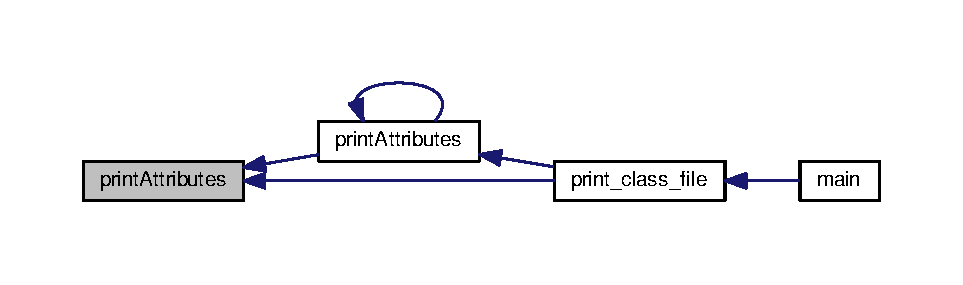
\includegraphics[width=350pt]{classfile_8c_af82a9138759e74a734c2ba5db6077805_icgraph}
\end{center}
\end{figure}


\index{classfile.\+c@{classfile.\+c}!print\+Const\+Type@{print\+Const\+Type}}
\index{print\+Const\+Type@{print\+Const\+Type}!classfile.\+c@{classfile.\+c}}
\subsubsection[{\texorpdfstring{print\+Const\+Type(u4 high\+\_\+bytes, u4 low\+\_\+bytes, u1 type)}{printConstType(u4 high_bytes, u4 low_bytes, u1 type)}}]{\setlength{\rightskip}{0pt plus 5cm}void print\+Const\+Type (
\begin{DoxyParamCaption}
\item[{{\bf u4}}]{high\+\_\+bytes, }
\item[{{\bf u4}}]{low\+\_\+bytes, }
\item[{{\bf u1}}]{type}
\end{DoxyParamCaption}
)}\hypertarget{classfile_8c_aa73a2b8f66296e2fcdec5b6f029c1f88}{}\label{classfile_8c_aa73a2b8f66296e2fcdec5b6f029c1f88}


Printa o tipo C\+O\+N\+S\+T\+A\+NT. 



Here is the caller graph for this function\+:
\nopagebreak
\begin{figure}[H]
\begin{center}
\leavevmode
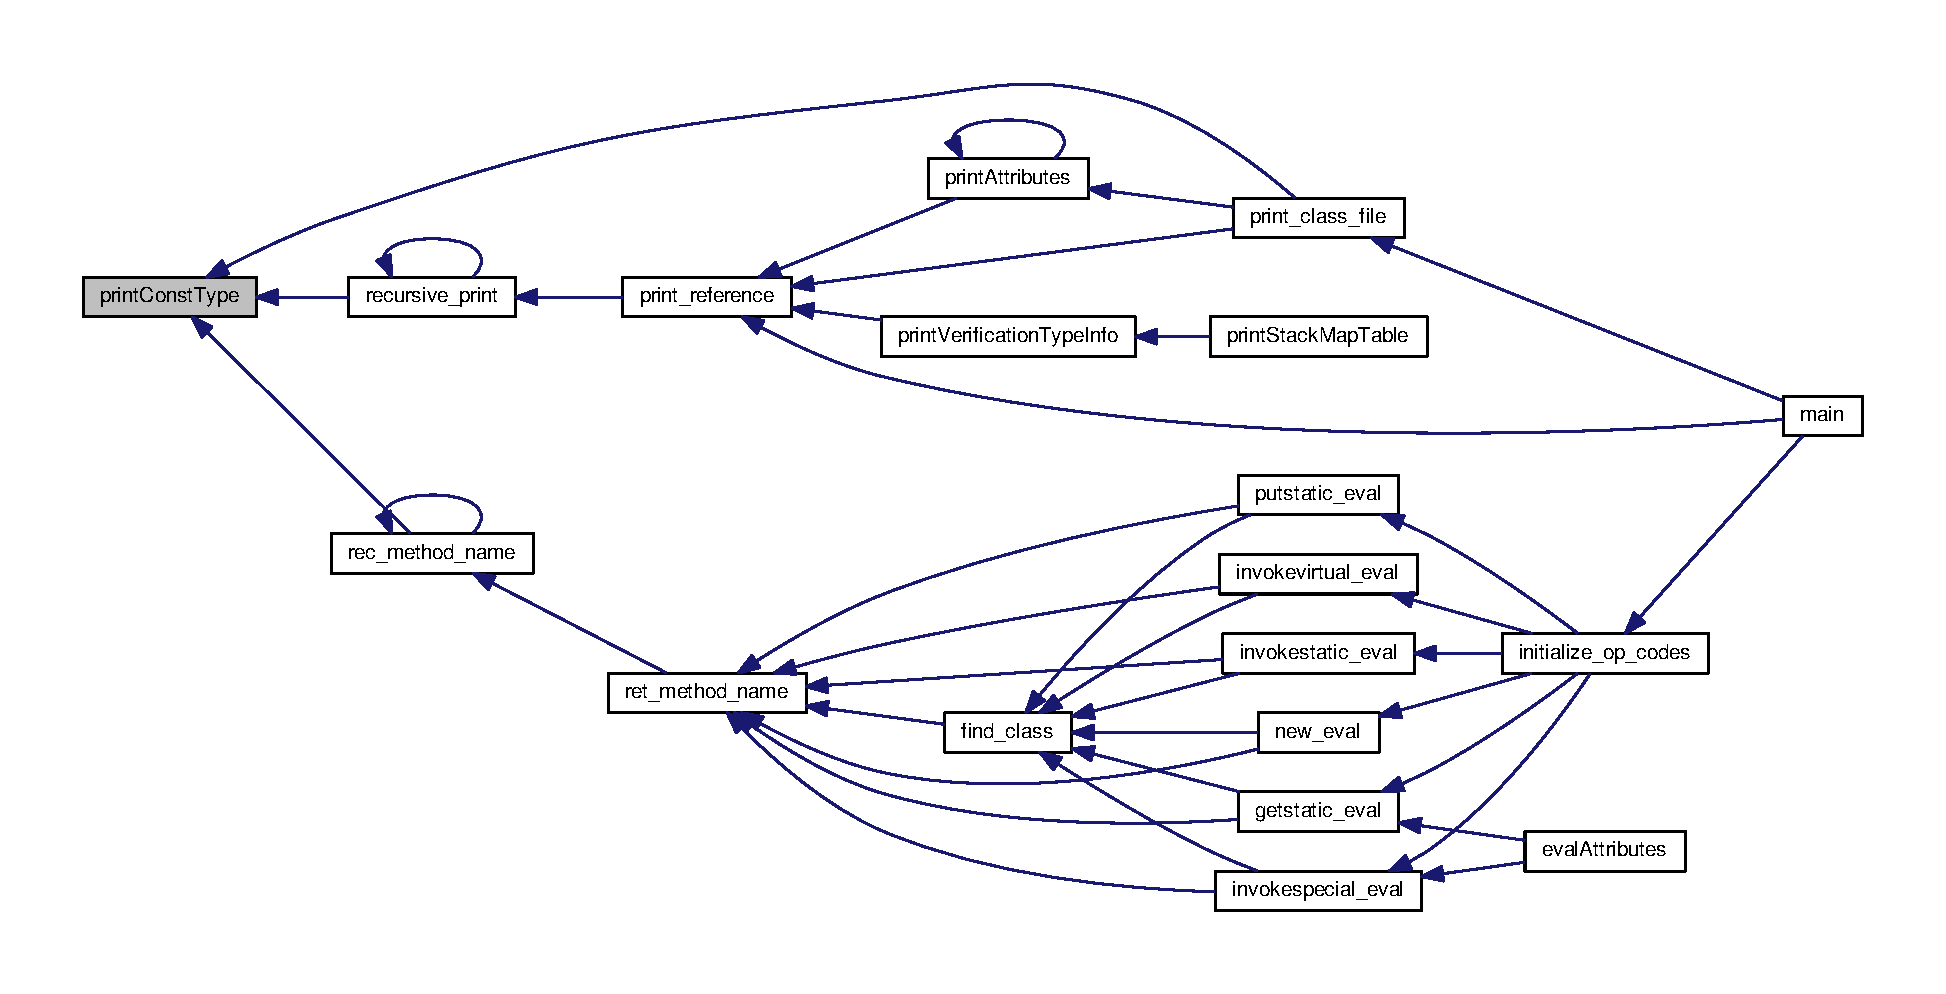
\includegraphics[width=350pt]{classfile_8c_aa73a2b8f66296e2fcdec5b6f029c1f88_icgraph}
\end{center}
\end{figure}


\index{classfile.\+c@{classfile.\+c}!print\+Flag@{print\+Flag}}
\index{print\+Flag@{print\+Flag}!classfile.\+c@{classfile.\+c}}
\subsubsection[{\texorpdfstring{print\+Flag(u2 type, u1 flag)}{printFlag(u2 type, u1 flag)}}]{\setlength{\rightskip}{0pt plus 5cm}char$\ast$ print\+Flag (
\begin{DoxyParamCaption}
\item[{{\bf u2}}]{type, }
\item[{{\bf u1}}]{flag}
\end{DoxyParamCaption}
)}\hypertarget{classfile_8c_a5636f6173ac96d0316cd018b68b34034}{}\label{classfile_8c_a5636f6173ac96d0316cd018b68b34034}


Printa a flag correspondente ao tipo recebido. 



Here is the caller graph for this function\+:
\nopagebreak
\begin{figure}[H]
\begin{center}
\leavevmode
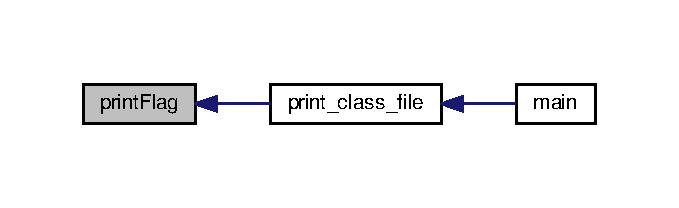
\includegraphics[width=326pt]{classfile_8c_a5636f6173ac96d0316cd018b68b34034_icgraph}
\end{center}
\end{figure}


\index{classfile.\+c@{classfile.\+c}!print\+Stack\+Map\+Table@{print\+Stack\+Map\+Table}}
\index{print\+Stack\+Map\+Table@{print\+Stack\+Map\+Table}!classfile.\+c@{classfile.\+c}}
\subsubsection[{\texorpdfstring{print\+Stack\+Map\+Table(stack\+\_\+map\+\_\+frame $\ast$stack\+\_\+map, cp\+\_\+info $\ast$cp, attribute\+\_\+info $\ast$attr)}{printStackMapTable(stack_map_frame *stack_map, cp_info *cp, attribute_info *attr)}}]{\setlength{\rightskip}{0pt plus 5cm}void print\+Stack\+Map\+Table (
\begin{DoxyParamCaption}
\item[{{\bf stack\+\_\+map\+\_\+frame} $\ast$}]{stack\+\_\+map, }
\item[{{\bf cp\+\_\+info} $\ast$}]{cp, }
\item[{{\bf attribute\+\_\+info} $\ast$}]{attr}
\end{DoxyParamCaption}
)}\hypertarget{classfile_8c_a08affa1a8eb0fbd41df9e468f2c02321}{}\label{classfile_8c_a08affa1a8eb0fbd41df9e468f2c02321}


Here is the call graph for this function\+:
\nopagebreak
\begin{figure}[H]
\begin{center}
\leavevmode
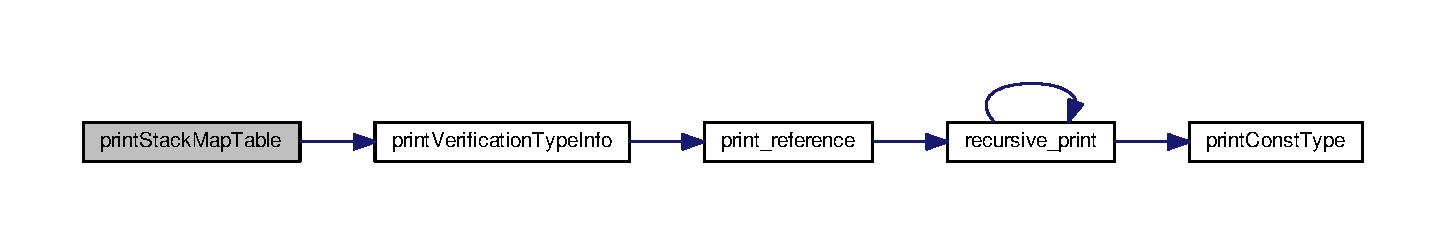
\includegraphics[width=350pt]{classfile_8c_a08affa1a8eb0fbd41df9e468f2c02321_cgraph}
\end{center}
\end{figure}


\index{classfile.\+c@{classfile.\+c}!print\+Type@{print\+Type}}
\index{print\+Type@{print\+Type}!classfile.\+c@{classfile.\+c}}
\subsubsection[{\texorpdfstring{print\+Type(u2 type)}{printType(u2 type)}}]{\setlength{\rightskip}{0pt plus 5cm}char$\ast$ print\+Type (
\begin{DoxyParamCaption}
\item[{{\bf u2}}]{type}
\end{DoxyParamCaption}
)}\hypertarget{classfile_8c_aae8cbe5dd2db133b98988d9da5c5efe7}{}\label{classfile_8c_aae8cbe5dd2db133b98988d9da5c5efe7}


Printa o tipo do objeto. 



Here is the caller graph for this function\+:
\nopagebreak
\begin{figure}[H]
\begin{center}
\leavevmode
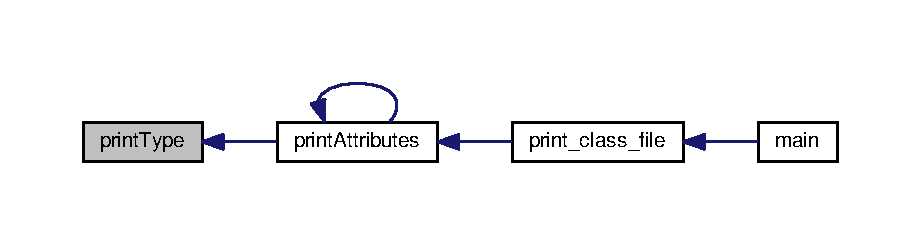
\includegraphics[width=350pt]{classfile_8c_aae8cbe5dd2db133b98988d9da5c5efe7_icgraph}
\end{center}
\end{figure}


\index{classfile.\+c@{classfile.\+c}!print\+Verification\+Type\+Info@{print\+Verification\+Type\+Info}}
\index{print\+Verification\+Type\+Info@{print\+Verification\+Type\+Info}!classfile.\+c@{classfile.\+c}}
\subsubsection[{\texorpdfstring{print\+Verification\+Type\+Info(verification\+\_\+type\+\_\+info $\ast$ver\+\_\+type, cp\+\_\+info $\ast$cp, u2 verification\+\_\+type\+\_\+length)}{printVerificationTypeInfo(verification_type_info *ver_type, cp_info *cp, u2 verification_type_length)}}]{\setlength{\rightskip}{0pt plus 5cm}void print\+Verification\+Type\+Info (
\begin{DoxyParamCaption}
\item[{{\bf verification\+\_\+type\+\_\+info} $\ast$}]{ver\+\_\+type, }
\item[{{\bf cp\+\_\+info} $\ast$}]{cp, }
\item[{{\bf u2}}]{verification\+\_\+type\+\_\+length}
\end{DoxyParamCaption}
)}\hypertarget{classfile_8c_ab694dc30480958e872cdf78b94b9cefa}{}\label{classfile_8c_ab694dc30480958e872cdf78b94b9cefa}


Printa o tipo a partir da tag. 



Here is the call graph for this function\+:
\nopagebreak
\begin{figure}[H]
\begin{center}
\leavevmode
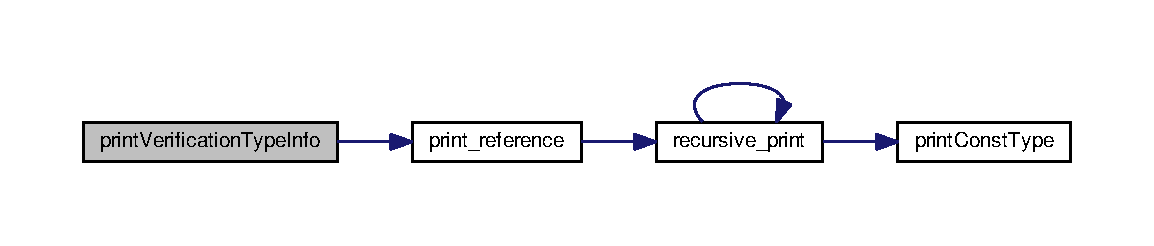
\includegraphics[width=350pt]{classfile_8c_ab694dc30480958e872cdf78b94b9cefa_cgraph}
\end{center}
\end{figure}




Here is the caller graph for this function\+:
\nopagebreak
\begin{figure}[H]
\begin{center}
\leavevmode
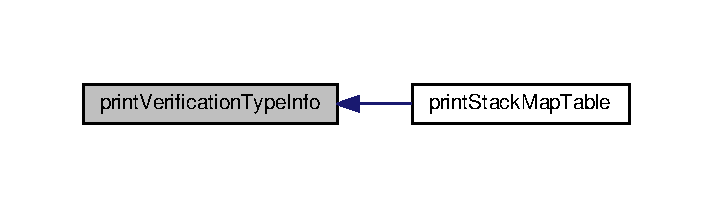
\includegraphics[width=342pt]{classfile_8c_ab694dc30480958e872cdf78b94b9cefa_icgraph}
\end{center}
\end{figure}


\index{classfile.\+c@{classfile.\+c}!print\+Version@{print\+Version}}
\index{print\+Version@{print\+Version}!classfile.\+c@{classfile.\+c}}
\subsubsection[{\texorpdfstring{print\+Version(u2 version)}{printVersion(u2 version)}}]{\setlength{\rightskip}{0pt plus 5cm}char$\ast$ print\+Version (
\begin{DoxyParamCaption}
\item[{{\bf u2}}]{version}
\end{DoxyParamCaption}
)}\hypertarget{classfile_8c_abbc0a67a74cf4718872b86f0a898575b}{}\label{classfile_8c_abbc0a67a74cf4718872b86f0a898575b}


Printa a versão do arquivo .class. 



Here is the caller graph for this function\+:
\nopagebreak
\begin{figure}[H]
\begin{center}
\leavevmode
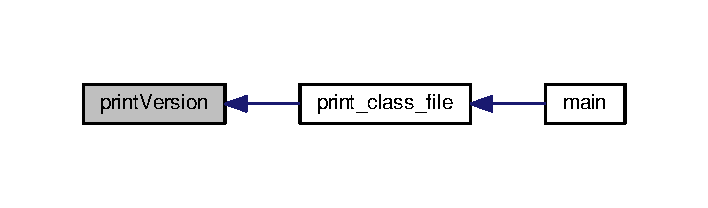
\includegraphics[width=340pt]{classfile_8c_abbc0a67a74cf4718872b86f0a898575b_icgraph}
\end{center}
\end{figure}


\index{classfile.\+c@{classfile.\+c}!read\+\_\+class\+\_\+file@{read\+\_\+class\+\_\+file}}
\index{read\+\_\+class\+\_\+file@{read\+\_\+class\+\_\+file}!classfile.\+c@{classfile.\+c}}
\subsubsection[{\texorpdfstring{read\+\_\+class\+\_\+file(\+Class\+File $\ast$cf, char $\ast$file\+\_\+name)}{read_class_file(ClassFile *cf, char *file_name)}}]{\setlength{\rightskip}{0pt plus 5cm}void read\+\_\+class\+\_\+file (
\begin{DoxyParamCaption}
\item[{{\bf Class\+File} $\ast$}]{cf, }
\item[{char $\ast$}]{file\+\_\+name}
\end{DoxyParamCaption}
)}\hypertarget{classfile_8c_a14c4d3f84dd03a43aca0a57bd530f3a2}{}\label{classfile_8c_a14c4d3f84dd03a43aca0a57bd530f3a2}


Faz a leitura do arquivo .class. 

Função principal de leitura. Recebe um ponteiro para uma struct do tipo \hyperlink{structcp__info}{cp\+\_\+info}, uma contagem do número de atributos e um ponteiro para o arquivo bytecodee raliza a leitura, byte a byte. 

Here is the call graph for this function\+:
\nopagebreak
\begin{figure}[H]
\begin{center}
\leavevmode
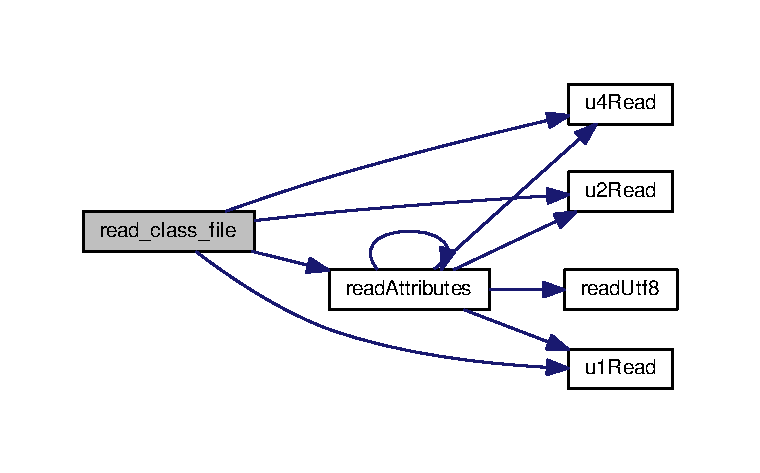
\includegraphics[width=350pt]{classfile_8c_a14c4d3f84dd03a43aca0a57bd530f3a2_cgraph}
\end{center}
\end{figure}




Here is the caller graph for this function\+:
\nopagebreak
\begin{figure}[H]
\begin{center}
\leavevmode
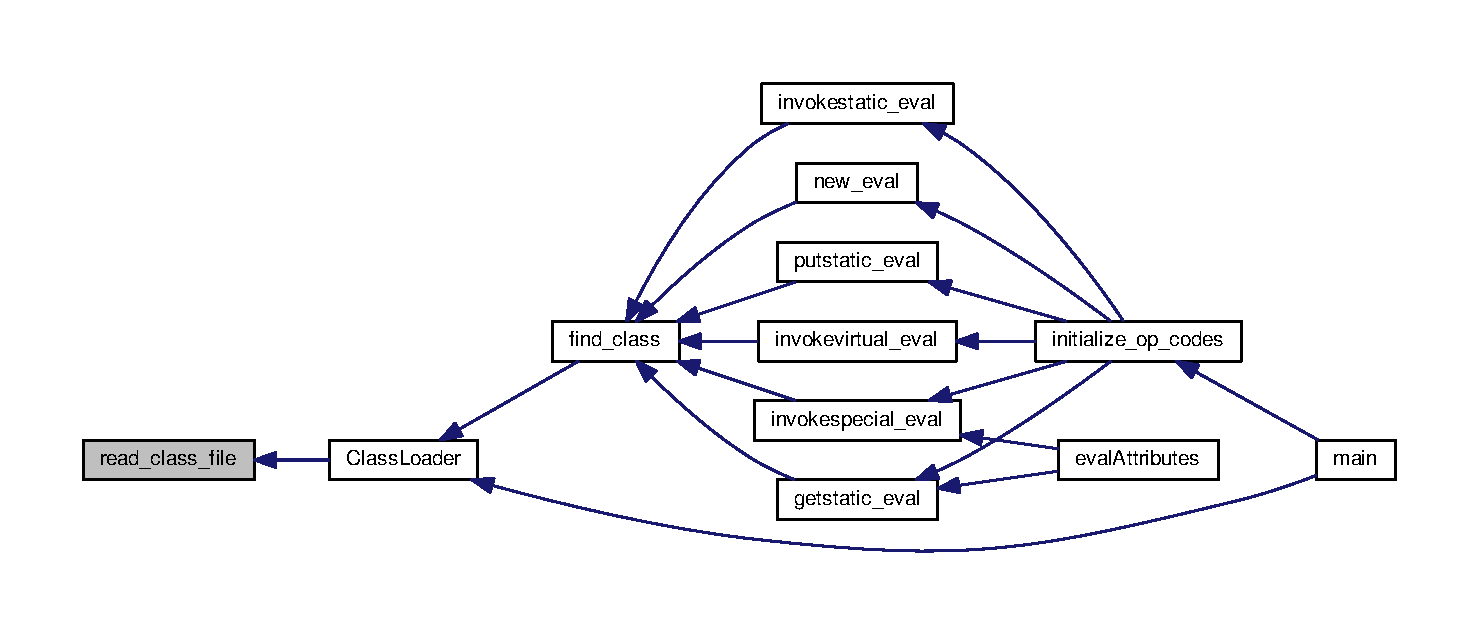
\includegraphics[width=350pt]{classfile_8c_a14c4d3f84dd03a43aca0a57bd530f3a2_icgraph}
\end{center}
\end{figure}


\index{classfile.\+c@{classfile.\+c}!read\+Attributes@{read\+Attributes}}
\index{read\+Attributes@{read\+Attributes}!classfile.\+c@{classfile.\+c}}
\subsubsection[{\texorpdfstring{read\+Attributes(cp\+\_\+info $\ast$cp, u2 attr\+\_\+count, F\+I\+L\+E $\ast$fp)}{readAttributes(cp_info *cp, u2 attr_count, FILE *fp)}}]{\setlength{\rightskip}{0pt plus 5cm}{\bf attribute\+\_\+info}$\ast$ read\+Attributes (
\begin{DoxyParamCaption}
\item[{{\bf cp\+\_\+info} $\ast$}]{cp, }
\item[{{\bf u2}}]{attr\+\_\+count, }
\item[{F\+I\+LE $\ast$}]{fp}
\end{DoxyParamCaption}
)}\hypertarget{classfile_8c_ab2c33d049c34b50ead32e4568387353c}{}\label{classfile_8c_ab2c33d049c34b50ead32e4568387353c}


Lê os atributos do bytecode recebido. 



Here is the call graph for this function\+:
\nopagebreak
\begin{figure}[H]
\begin{center}
\leavevmode
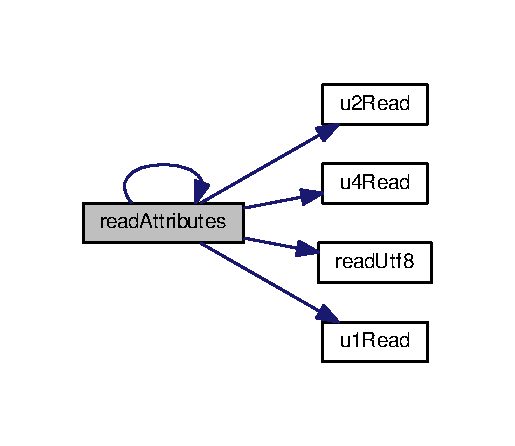
\includegraphics[width=247pt]{classfile_8c_ab2c33d049c34b50ead32e4568387353c_cgraph}
\end{center}
\end{figure}




Here is the caller graph for this function\+:
\nopagebreak
\begin{figure}[H]
\begin{center}
\leavevmode
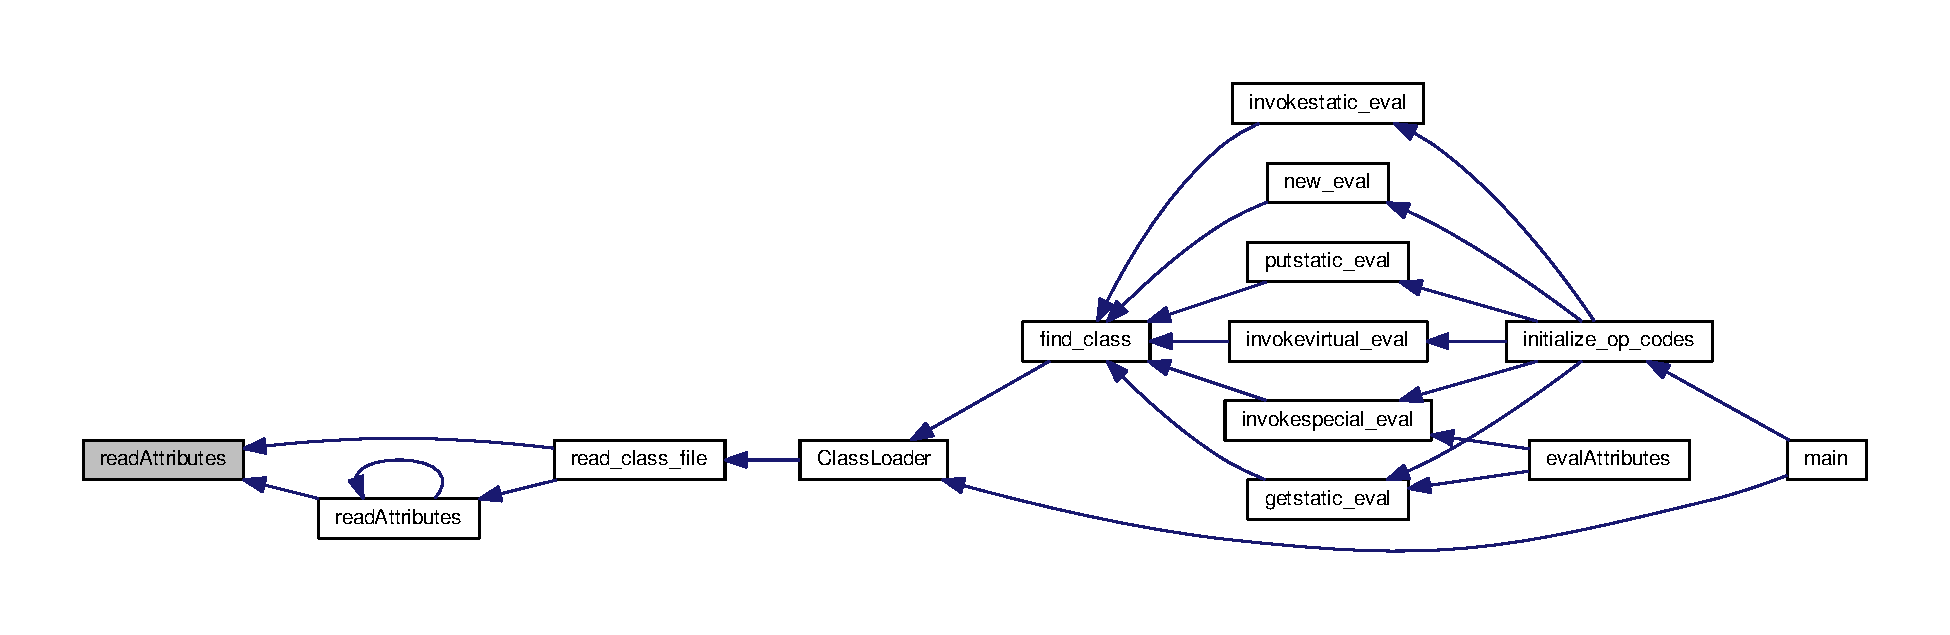
\includegraphics[width=350pt]{classfile_8c_ab2c33d049c34b50ead32e4568387353c_icgraph}
\end{center}
\end{figure}


\index{classfile.\+c@{classfile.\+c}!read\+Utf8@{read\+Utf8}}
\index{read\+Utf8@{read\+Utf8}!classfile.\+c@{classfile.\+c}}
\subsubsection[{\texorpdfstring{read\+Utf8(cp\+\_\+info $\ast$cp, u2 index)}{readUtf8(cp_info *cp, u2 index)}}]{\setlength{\rightskip}{0pt plus 5cm}char$\ast$ read\+Utf8 (
\begin{DoxyParamCaption}
\item[{{\bf cp\+\_\+info} $\ast$}]{cp, }
\item[{{\bf u2}}]{index}
\end{DoxyParamCaption}
)}\hypertarget{classfile_8c_a77c5107c582c86dedb65853efabd9302}{}\label{classfile_8c_a77c5107c582c86dedb65853efabd9302}


Faz a leitua dos bytes no formato U\+T\+F-\/8. 



Here is the caller graph for this function\+:
\nopagebreak
\begin{figure}[H]
\begin{center}
\leavevmode
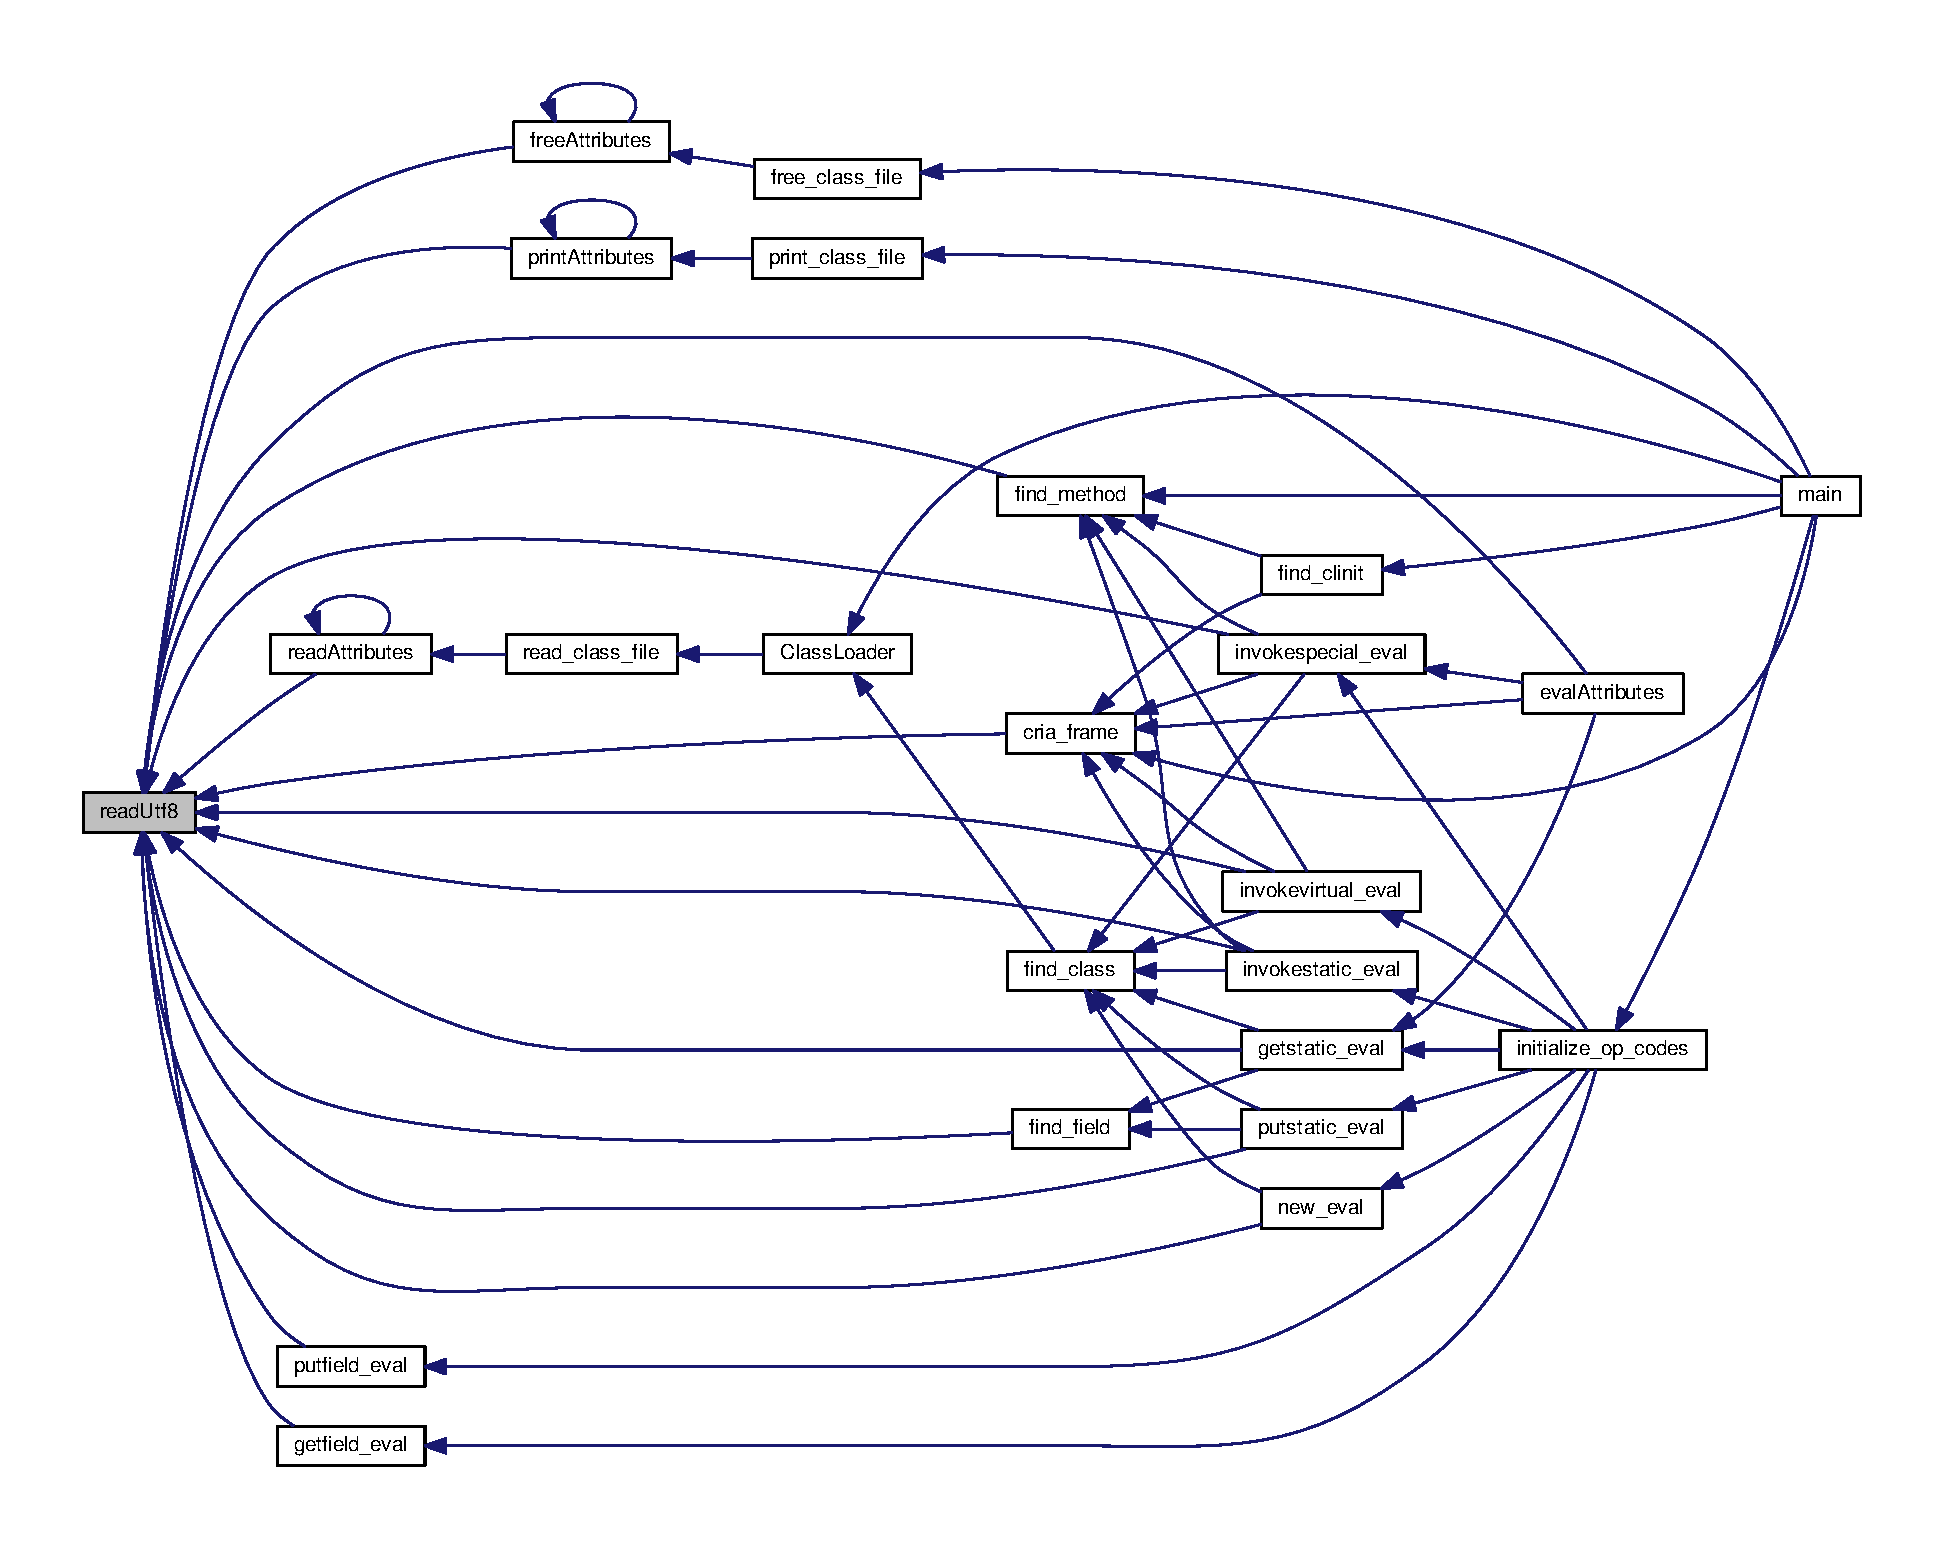
\includegraphics[width=350pt]{classfile_8c_a77c5107c582c86dedb65853efabd9302_icgraph}
\end{center}
\end{figure}


\index{classfile.\+c@{classfile.\+c}!rec\+\_\+method\+\_\+name@{rec\+\_\+method\+\_\+name}}
\index{rec\+\_\+method\+\_\+name@{rec\+\_\+method\+\_\+name}!classfile.\+c@{classfile.\+c}}
\subsubsection[{\texorpdfstring{rec\+\_\+method\+\_\+name(cp\+\_\+info $\ast$cp, u2 index)}{rec_method_name(cp_info *cp, u2 index)}}]{\setlength{\rightskip}{0pt plus 5cm}char$\ast$ rec\+\_\+method\+\_\+name (
\begin{DoxyParamCaption}
\item[{{\bf cp\+\_\+info} $\ast$}]{cp, }
\item[{{\bf u2}}]{index}
\end{DoxyParamCaption}
)}\hypertarget{classfile_8c_a580d63d9a7b152364691f69863dc7a4e}{}\label{classfile_8c_a580d63d9a7b152364691f69863dc7a4e}


Usa um índice no constant pool para procurar o nome de um método recursivamente. 



Here is the call graph for this function\+:
\nopagebreak
\begin{figure}[H]
\begin{center}
\leavevmode
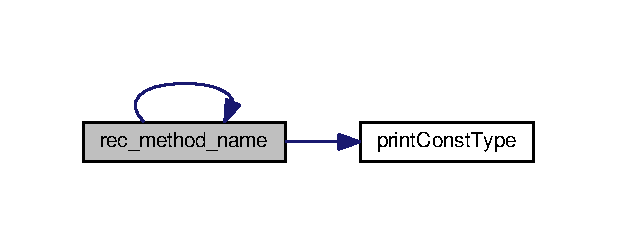
\includegraphics[width=296pt]{classfile_8c_a580d63d9a7b152364691f69863dc7a4e_cgraph}
\end{center}
\end{figure}




Here is the caller graph for this function\+:
\nopagebreak
\begin{figure}[H]
\begin{center}
\leavevmode
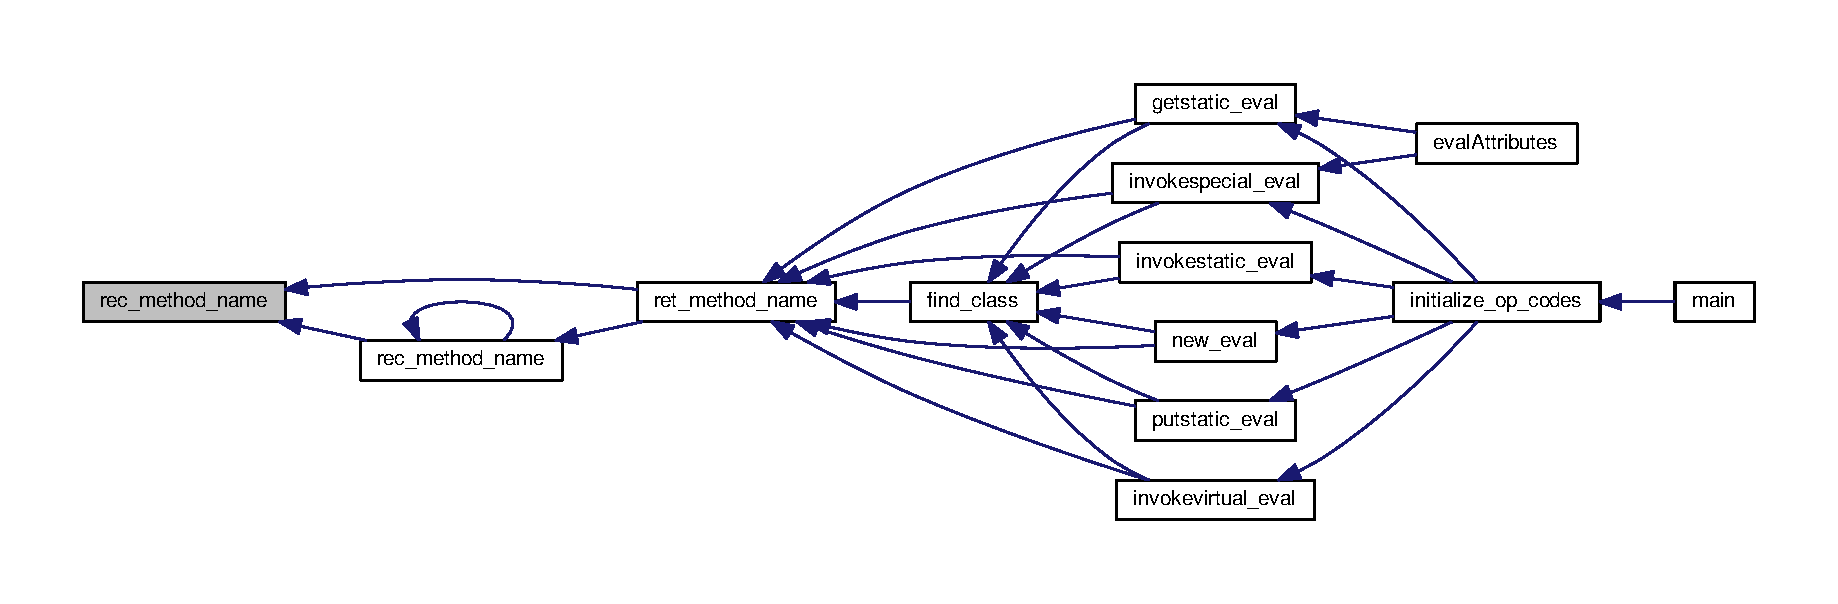
\includegraphics[width=350pt]{classfile_8c_a580d63d9a7b152364691f69863dc7a4e_icgraph}
\end{center}
\end{figure}


\index{classfile.\+c@{classfile.\+c}!recursive\+\_\+print@{recursive\+\_\+print}}
\index{recursive\+\_\+print@{recursive\+\_\+print}!classfile.\+c@{classfile.\+c}}
\subsubsection[{\texorpdfstring{recursive\+\_\+print(cp\+\_\+info $\ast$cp, u2 index, char $\ast$str)}{recursive_print(cp_info *cp, u2 index, char *str)}}]{\setlength{\rightskip}{0pt plus 5cm}void recursive\+\_\+print (
\begin{DoxyParamCaption}
\item[{{\bf cp\+\_\+info} $\ast$}]{cp, }
\item[{{\bf u2}}]{index, }
\item[{char $\ast$}]{str}
\end{DoxyParamCaption}
)}\hypertarget{classfile_8c_a774f5149d9c3dadc60b2c0ca012bf51d}{}\label{classfile_8c_a774f5149d9c3dadc60b2c0ca012bf51d}


Usa um índice para acessar a constant pool e printar recusrivamente os campos. 



Here is the call graph for this function\+:
\nopagebreak
\begin{figure}[H]
\begin{center}
\leavevmode
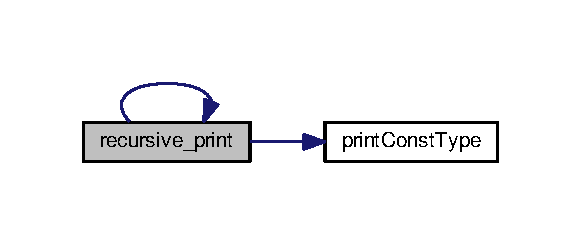
\includegraphics[width=279pt]{classfile_8c_a774f5149d9c3dadc60b2c0ca012bf51d_cgraph}
\end{center}
\end{figure}




Here is the caller graph for this function\+:
\nopagebreak
\begin{figure}[H]
\begin{center}
\leavevmode
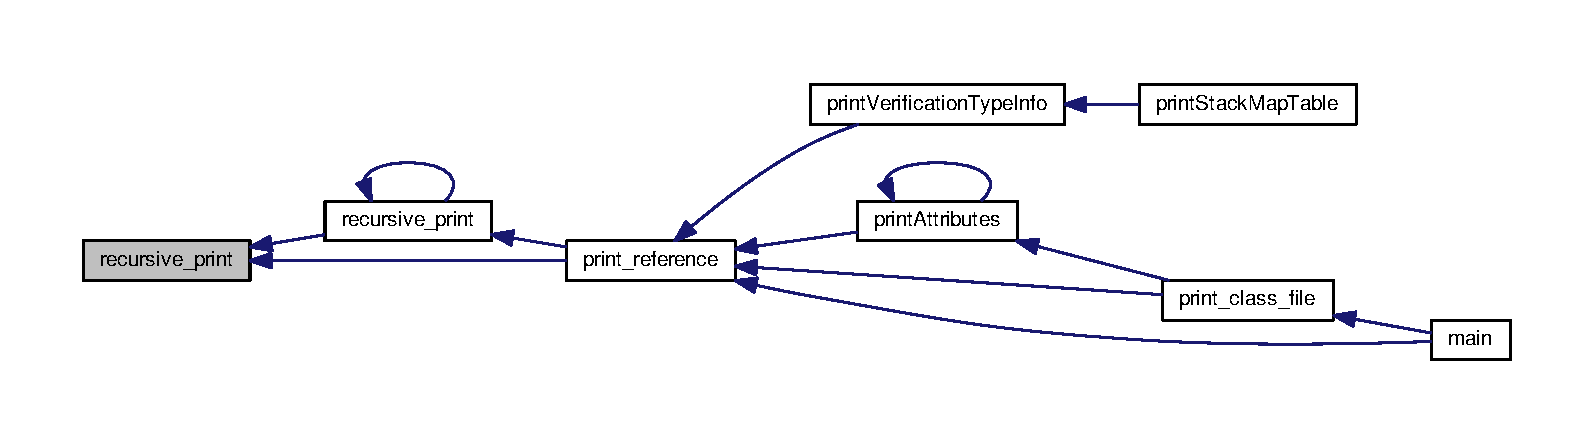
\includegraphics[width=350pt]{classfile_8c_a774f5149d9c3dadc60b2c0ca012bf51d_icgraph}
\end{center}
\end{figure}


\index{classfile.\+c@{classfile.\+c}!remove\+Extension@{remove\+Extension}}
\index{remove\+Extension@{remove\+Extension}!classfile.\+c@{classfile.\+c}}
\subsubsection[{\texorpdfstring{remove\+Extension(char $\ast$string)}{removeExtension(char *string)}}]{\setlength{\rightskip}{0pt plus 5cm}char$\ast$ remove\+Extension (
\begin{DoxyParamCaption}
\item[{char $\ast$}]{string}
\end{DoxyParamCaption}
)}\hypertarget{classfile_8c_af82954dceccc52fab4a547f79967244f}{}\label{classfile_8c_af82954dceccc52fab4a547f79967244f}


Remove exetensão de uma string para printar de maneira correta. 



Here is the caller graph for this function\+:
\nopagebreak
\begin{figure}[H]
\begin{center}
\leavevmode
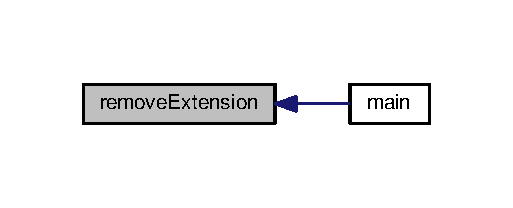
\includegraphics[width=246pt]{classfile_8c_af82954dceccc52fab4a547f79967244f_icgraph}
\end{center}
\end{figure}


\index{classfile.\+c@{classfile.\+c}!ret\+\_\+method\+\_\+name@{ret\+\_\+method\+\_\+name}}
\index{ret\+\_\+method\+\_\+name@{ret\+\_\+method\+\_\+name}!classfile.\+c@{classfile.\+c}}
\subsubsection[{\texorpdfstring{ret\+\_\+method\+\_\+name(cp\+\_\+info $\ast$cp, u2 index)}{ret_method_name(cp_info *cp, u2 index)}}]{\setlength{\rightskip}{0pt plus 5cm}char$\ast$ ret\+\_\+method\+\_\+name (
\begin{DoxyParamCaption}
\item[{{\bf cp\+\_\+info} $\ast$}]{cp, }
\item[{{\bf u2}}]{index}
\end{DoxyParamCaption}
)}\hypertarget{classfile_8c_a627193785e98bc076b257c97ccd5892b}{}\label{classfile_8c_a627193785e98bc076b257c97ccd5892b}


Retorna o nome de um método no ponteiro global. 



Here is the call graph for this function\+:
\nopagebreak
\begin{figure}[H]
\begin{center}
\leavevmode
\includegraphics[width=350pt]{classfile_8c_a627193785e98bc076b257c97ccd5892b_cgraph}
\end{center}
\end{figure}




Here is the caller graph for this function\+:
\nopagebreak
\begin{figure}[H]
\begin{center}
\leavevmode
\includegraphics[width=350pt]{classfile_8c_a627193785e98bc076b257c97ccd5892b_icgraph}
\end{center}
\end{figure}


\index{classfile.\+c@{classfile.\+c}!u1\+Read@{u1\+Read}}
\index{u1\+Read@{u1\+Read}!classfile.\+c@{classfile.\+c}}
\subsubsection[{\texorpdfstring{u1\+Read(\+F\+I\+L\+E $\ast$file)}{u1Read(FILE *file)}}]{\setlength{\rightskip}{0pt plus 5cm}{\bf u1} u1\+Read (
\begin{DoxyParamCaption}
\item[{F\+I\+LE $\ast$}]{file}
\end{DoxyParamCaption}
)}\hypertarget{classfile_8c_a13b463381f7cf580d002e6631c0c4ea8}{}\label{classfile_8c_a13b463381f7cf580d002e6631c0c4ea8}


Faz a leitura de 1 byte do arquivo .class fornecido no path. 



Here is the caller graph for this function\+:
\nopagebreak
\begin{figure}[H]
\begin{center}
\leavevmode
\includegraphics[width=350pt]{classfile_8c_a13b463381f7cf580d002e6631c0c4ea8_icgraph}
\end{center}
\end{figure}


\index{classfile.\+c@{classfile.\+c}!u2\+Read@{u2\+Read}}
\index{u2\+Read@{u2\+Read}!classfile.\+c@{classfile.\+c}}
\subsubsection[{\texorpdfstring{u2\+Read(\+F\+I\+L\+E $\ast$file)}{u2Read(FILE *file)}}]{\setlength{\rightskip}{0pt plus 5cm}{\bf u2} u2\+Read (
\begin{DoxyParamCaption}
\item[{F\+I\+LE $\ast$}]{file}
\end{DoxyParamCaption}
)}\hypertarget{classfile_8c_aae51575c6f1d6ce808fbc88a3037c4ed}{}\label{classfile_8c_aae51575c6f1d6ce808fbc88a3037c4ed}


Faz a leitura de 2 bytes do arquivo .class fornecido no path. 



Here is the caller graph for this function\+:
\nopagebreak
\begin{figure}[H]
\begin{center}
\leavevmode
\includegraphics[width=350pt]{classfile_8c_aae51575c6f1d6ce808fbc88a3037c4ed_icgraph}
\end{center}
\end{figure}


\index{classfile.\+c@{classfile.\+c}!u4\+Read@{u4\+Read}}
\index{u4\+Read@{u4\+Read}!classfile.\+c@{classfile.\+c}}
\subsubsection[{\texorpdfstring{u4\+Read(\+F\+I\+L\+E $\ast$file)}{u4Read(FILE *file)}}]{\setlength{\rightskip}{0pt plus 5cm}{\bf u4} u4\+Read (
\begin{DoxyParamCaption}
\item[{F\+I\+LE $\ast$}]{file}
\end{DoxyParamCaption}
)}\hypertarget{classfile_8c_aad8c26a8aaff63010bb790df878f0950}{}\label{classfile_8c_aad8c26a8aaff63010bb790df878f0950}


Faz a leitura de 4 bytes do arquivo .class fornecido no path. 



Here is the caller graph for this function\+:
\nopagebreak
\begin{figure}[H]
\begin{center}
\leavevmode
\includegraphics[width=350pt]{classfile_8c_aad8c26a8aaff63010bb790df878f0950_icgraph}
\end{center}
\end{figure}



\hypertarget{classfile_8h}{}\section{classfile.\+h File Reference}
\label{classfile_8h}\index{classfile.\+h@{classfile.\+h}}
{\ttfamily \#include $<$stdio.\+h$>$}\\*
{\ttfamily \#include \char`\"{}structures.\+h\char`\"{}}\\*
{\ttfamily \#include \char`\"{}stack\+\_\+frame.\+h\char`\"{}}\\*
Include dependency graph for classfile.\+h\+:
% FIG 0
This graph shows which files directly or indirectly include this file\+:
% FIG 1
\subsection*{Functions}
\begin{DoxyCompactItemize}
\item 
\hyperlink{structures_8h_a64f8055b64cf2a4c299c841130c5c938}{u1} \hyperlink{classfile_8h_a39801833579e32d1d5c844229c82cef1}{u1\+Read} (F\+I\+LE $\ast$)
\begin{DoxyCompactList}\small\item\em Faz a leitura de 1 byte do arquivo .class fornecido no path. \end{DoxyCompactList}\item 
\hyperlink{structures_8h_a55ef8d87fd202b8417704c089899c5b9}{u2} \hyperlink{classfile_8h_a88e62d36ef0e91dda130024e0b07dff2}{u2\+Read} (F\+I\+LE $\ast$)
\begin{DoxyCompactList}\small\item\em Faz a leitura de 2 bytes do arquivo .class fornecido no path. \end{DoxyCompactList}\item 
\hyperlink{structures_8h_ae391a1d79bb0c8cbc283f0283e3c098b}{u4} \hyperlink{classfile_8h_a53b3222e2a57ce27a8ad7a04a35f8f6e}{u4\+Read} (F\+I\+LE $\ast$)
\begin{DoxyCompactList}\small\item\em Faz a leitura de 4 bytes do arquivo .class fornecido no path. \end{DoxyCompactList}\item 
void \hyperlink{classfile_8h_a14c4d3f84dd03a43aca0a57bd530f3a2}{read\+\_\+class\+\_\+file} (\hyperlink{structClassFile}{Class\+File} $\ast$cf, char $\ast$file\+\_\+name)
\begin{DoxyCompactList}\small\item\em Faz a leitura do arquivo .class. \end{DoxyCompactList}\item 
void \hyperlink{classfile_8h_a67e8b211dae28d036af3a55b698da993}{print\+\_\+class\+\_\+file} (\hyperlink{structClassFile}{Class\+File} $\ast$cf)
\begin{DoxyCompactList}\small\item\em Recebe um classfile como parâmetro e printa seu conteúdo de maneira organizada no terminal. (Utilizado pelo leitor/exibidor de bytecode). \end{DoxyCompactList}\item 
void \hyperlink{classfile_8h_a6a7ca9bbe1c17ec34271f8c898832ee0}{free\+\_\+class\+\_\+file} (\hyperlink{structClassFile}{Class\+File} $\ast$cf)
\begin{DoxyCompactList}\small\item\em Libera o classfile da memória. \end{DoxyCompactList}\item 
char $\ast$ \hyperlink{classfile_8h_a77c5107c582c86dedb65853efabd9302}{read\+Utf8} (\hyperlink{structcp__info}{cp\+\_\+info} $\ast$cp, \hyperlink{structures_8h_a55ef8d87fd202b8417704c089899c5b9}{u2} index)
\begin{DoxyCompactList}\small\item\em Faz a leitua dos bytes no formato U\+T\+F-\/8. \end{DoxyCompactList}\item 
\hyperlink{structattribute__info}{attribute\+\_\+info} $\ast$ \hyperlink{classfile_8h_ab2c33d049c34b50ead32e4568387353c}{read\+Attributes} (\hyperlink{structcp__info}{cp\+\_\+info} $\ast$cp, \hyperlink{structures_8h_a55ef8d87fd202b8417704c089899c5b9}{u2} attr\+\_\+count, F\+I\+LE $\ast$fp)
\begin{DoxyCompactList}\small\item\em Lê os atributos do bytecode recebido. \end{DoxyCompactList}\item 
void \hyperlink{classfile_8h_af82a9138759e74a734c2ba5db6077805}{print\+Attributes} (\hyperlink{structattribute__info}{attribute\+\_\+info} $\ast$field, \hyperlink{structcp__info}{cp\+\_\+info} $\ast$cp, \hyperlink{structures_8h_a55ef8d87fd202b8417704c089899c5b9}{u2} attr\+\_\+count)
\begin{DoxyCompactList}\small\item\em Printa os atributos de um classfile. \end{DoxyCompactList}\item 
void \hyperlink{classfile_8h_a8d5e46a5df7dfb965306e8a277783511}{eval\+Attributes} (\hyperlink{structattribute__info}{attribute\+\_\+info} $\ast$field, \hyperlink{structcp__info}{cp\+\_\+info} $\ast$cp, \hyperlink{structures_8h_a55ef8d87fd202b8417704c089899c5b9}{u2} attr\+\_\+count, \hyperlink{structClassFile}{Class\+File} $\ast$cf)
\begin{DoxyCompactList}\small\item\em todo\+: avalia os atributos do classfile. \end{DoxyCompactList}\item 
void \hyperlink{classfile_8h_a774f5149d9c3dadc60b2c0ca012bf51d}{recursive\+\_\+print} (\hyperlink{structcp__info}{cp\+\_\+info} $\ast$cp, \hyperlink{structures_8h_a55ef8d87fd202b8417704c089899c5b9}{u2} index, char $\ast$str)
\begin{DoxyCompactList}\small\item\em Usa um índice para acessar a constant pool e printar recusrivamente os campos. \end{DoxyCompactList}\item 
void \hyperlink{classfile_8h_aa368bab42b5e8b5415b68d6910982ea2}{rec\+\_\+method\+\_\+name} (\hyperlink{structcp__info}{cp\+\_\+info} $\ast$cp, \hyperlink{structures_8h_a55ef8d87fd202b8417704c089899c5b9}{u2} index, char $\ast$str)
\begin{DoxyCompactList}\small\item\em Usa um índice no constant pool para procurar o nome de um método recursivamente. \end{DoxyCompactList}\item 
char $\ast$ \hyperlink{classfile_8h_a627193785e98bc076b257c97ccd5892b}{ret\+\_\+method\+\_\+name} (\hyperlink{structcp__info}{cp\+\_\+info} $\ast$cp, \hyperlink{structures_8h_a55ef8d87fd202b8417704c089899c5b9}{u2} index)
\begin{DoxyCompactList}\small\item\em Retorna o nome de um método no ponteiro global. \end{DoxyCompactList}\item 
char $\ast$ \hyperlink{classfile_8h_a09f80f214aa870612fcb23597bcfb4bc}{print\+\_\+reference} (\hyperlink{structcp__info}{cp\+\_\+info} $\ast$cp, \hyperlink{structures_8h_a55ef8d87fd202b8417704c089899c5b9}{u2} index)
\begin{DoxyCompactList}\small\item\em Usa um índice na constant pool para retorna uma referência no ponteiro global. \end{DoxyCompactList}\item 
\hyperlink{structverification__type__info}{verification\+\_\+type\+\_\+info} $\ast$ \hyperlink{classfile_8h_add61e24daf8356973e908b3f1cfd5a24}{fill\+Verification\+Type\+Info} (F\+I\+LE $\ast$fp, \hyperlink{structures_8h_a55ef8d87fd202b8417704c089899c5b9}{u2} verification\+\_\+type\+\_\+length)
\begin{DoxyCompactList}\small\item\em Faz a leitura de 1 byre do arquivo .class fornecido no path. \end{DoxyCompactList}\item 
\hyperlink{structstack__map__frame}{stack\+\_\+map\+\_\+frame} $\ast$ \hyperlink{classfile_8h_a1258b84eec00db8fee377fea434c49b1}{fill\+Stack\+Map\+Table} (\hyperlink{structattribute__info}{attribute\+\_\+info} $\ast$attr, F\+I\+LE $\ast$fp)
\item 
void \hyperlink{classfile_8h_a3bfb911a1e769d93bb0e18492aab956b}{free\+Attributes} (\hyperlink{structattribute__info}{attribute\+\_\+info} $\ast$field, \hyperlink{structcp__info}{cp\+\_\+info} $\ast$cp, \hyperlink{structures_8h_a55ef8d87fd202b8417704c089899c5b9}{u2} attr\+\_\+count)
\begin{DoxyCompactList}\small\item\em Função utilizada para liberar a memória ocupada pelo classfile. \end{DoxyCompactList}\item 
void \hyperlink{classfile_8h_ab694dc30480958e872cdf78b94b9cefa}{print\+Verification\+Type\+Info} (\hyperlink{structverification__type__info}{verification\+\_\+type\+\_\+info} $\ast$ver\+\_\+type, \hyperlink{structcp__info}{cp\+\_\+info} $\ast$cp, \hyperlink{structures_8h_a55ef8d87fd202b8417704c089899c5b9}{u2} verification\+\_\+type\+\_\+length)
\begin{DoxyCompactList}\small\item\em Printa o tipo a partir da tag. \end{DoxyCompactList}\item 
void \hyperlink{classfile_8h_a08affa1a8eb0fbd41df9e468f2c02321}{print\+Stack\+Map\+Table} (\hyperlink{structstack__map__frame}{stack\+\_\+map\+\_\+frame} $\ast$stack\+\_\+map, \hyperlink{structcp__info}{cp\+\_\+info} $\ast$cp, \hyperlink{structattribute__info}{attribute\+\_\+info} $\ast$attr)
\item 
void \hyperlink{classfile_8h_ac72c096a138416b9909fe3e29417763e}{free\+Stack\+Map\+Table} (\hyperlink{structstack__map__frame}{stack\+\_\+map\+\_\+frame} $\ast$stack\+\_\+map, \hyperlink{structattribute__info}{attribute\+\_\+info} $\ast$attr)
\item 
void \hyperlink{classfile_8h_aa73a2b8f66296e2fcdec5b6f029c1f88}{print\+Const\+Type} (\hyperlink{structures_8h_ae391a1d79bb0c8cbc283f0283e3c098b}{u4} high\+\_\+bytes, \hyperlink{structures_8h_ae391a1d79bb0c8cbc283f0283e3c098b}{u4} low\+\_\+bytes, \hyperlink{structures_8h_a64f8055b64cf2a4c299c841130c5c938}{u1} type)
\begin{DoxyCompactList}\small\item\em Printa o tipo C\+O\+N\+S\+T\+A\+NT. \end{DoxyCompactList}\item 
char $\ast$ \hyperlink{classfile_8h_a5636f6173ac96d0316cd018b68b34034}{print\+Flag} (\hyperlink{structures_8h_a55ef8d87fd202b8417704c089899c5b9}{u2} type, \hyperlink{structures_8h_a64f8055b64cf2a4c299c841130c5c938}{u1} flag)
\begin{DoxyCompactList}\small\item\em Printa a flag correspondente ao tipo recebido. \end{DoxyCompactList}\item 
char $\ast$ \hyperlink{classfile_8h_abbc0a67a74cf4718872b86f0a898575b}{print\+Version} (\hyperlink{structures_8h_a55ef8d87fd202b8417704c089899c5b9}{u2} version)
\begin{DoxyCompactList}\small\item\em Printa a versão do arquivo .class. \end{DoxyCompactList}\item 
char $\ast$ \hyperlink{classfile_8h_af82954dceccc52fab4a547f79967244f}{remove\+Extension} (char $\ast$string)
\begin{DoxyCompactList}\small\item\em Remove exetensão de uma string para printar de maneira correta. \end{DoxyCompactList}\item 
char $\ast$ \hyperlink{classfile_8h_a50ab5cb2c7741908305afda2e2a0235a}{find\+Name\+File} (char $\ast$string)
\item 
\hyperlink{structures_8h_ae391a1d79bb0c8cbc283f0283e3c098b}{u4} \hyperlink{classfile_8h_abd0631a75f72632c5606e72f6d3f00ae}{Class\+Loader} (char $\ast$class\+\_\+name)
\begin{DoxyCompactList}\small\item\em Aloca espaço para o \hyperlink{structClassFile}{Class\+File} em memória e chama a função read\+\_\+class\+\_\+file para ler o \hyperlink{structClassFile}{Class\+File} recebido nas posições corretas. \end{DoxyCompactList}\item 
void \hyperlink{classfile_8h_a55c80ae86c1c6d0666108a825df64a4b}{execute\+\_\+gvm} ()
\begin{DoxyCompactList}\small\item\em Função que busca pelo \hyperlink{structFrame}{Frame} no topo da pilha de frames e inicia a execução da \hyperlink{structJVM}{J\+VM}. Essa função é executada enquanto ainda há frames na pilha da \hyperlink{structJVM}{J\+VM}. \end{DoxyCompactList}\item 
\hyperlink{structmethod__info}{method\+\_\+info} $\ast$ \hyperlink{classfile_8h_acaf2255d12202a819c765194e5e51dba}{find\+\_\+method} (\hyperlink{structClassFile}{Class\+File} $\ast$cf, char $\ast$method)
\begin{DoxyCompactList}\small\item\em Procura por um método dentro do Classfile carregado em memória. \end{DoxyCompactList}\item 
\hyperlink{structures_8h_a55ef8d87fd202b8417704c089899c5b9}{u2} \hyperlink{classfile_8h_a64bd697d9f3c3360d6c4edb38f8cdf60}{find\+\_\+class} (char $\ast$class\+\_\+name)
\begin{DoxyCompactList}\small\item\em Procura por cuma classe, e caso não consiga encontrá-\/la, carrega na memória usando a função Class\+Loader. \end{DoxyCompactList}\item 
\hyperlink{structfield__info}{field\+\_\+info} $\ast$ \hyperlink{classfile_8h_a0688afe113144b86408f83f83685db04}{find\+\_\+field} (\hyperlink{structClassFile}{Class\+File} $\ast$cf, char $\ast$field\+\_\+name, char $\ast$field\+\_\+desc)
\begin{DoxyCompactList}\small\item\em Procura por um field dentro do \hyperlink{structClassFile}{Class\+File}. \end{DoxyCompactList}\item 
void \hyperlink{classfile_8h_a39063f00cc6ccce0402e1a81f2f760af}{find\+\_\+clinit} (\hyperlink{structClassFile}{Class\+File} $\ast$cf)
\begin{DoxyCompactList}\small\item\em Procura por um init dentro do Classfile. \end{DoxyCompactList}\end{DoxyCompactItemize}
\subsection*{Variables}
\begin{DoxyCompactItemize}
\item 
char $\ast$ \hyperlink{classfile_8h_a17dd988cd7a015cb95f53b4dcfd5842a}{G\+L\+O\+B\+A\+L\+\_\+ptr}
\item 
\hyperlink{structures_8h_a64f8055b64cf2a4c299c841130c5c938}{u1} \hyperlink{classfile_8h_aa38db19f7894f13a48f3f8c0b062549b}{code\+\_\+sep}
\item 
\hyperlink{structures_8h_a64f8055b64cf2a4c299c841130c5c938}{u1} \hyperlink{classfile_8h_a1aeea90933b6eec3bb962639e5e0b3fa}{name\+\_\+or\+\_\+type}
\item 
char $\ast$ \hyperlink{classfile_8h_a5ba9132e7f1a55a732182a4ae2b80cf7}{F\+I\+L\+E\+\_\+\+N\+A\+ME}
\item 
\hyperlink{structStackFrame}{Stack\+Frame} $\ast$ \hyperlink{classfile_8h_a15f64dbdb65ef3f2f338253004e88b99}{Jvm\+Stack}
\item 
\hyperlink{structMethod}{Method} \hyperlink{classfile_8h_aacaf45a8478861c2788165e9f0d24a3c}{Mem}
\end{DoxyCompactItemize}


\subsection{Function Documentation}
\index{classfile.\+h@{classfile.\+h}!Class\+Loader@{Class\+Loader}}
\index{Class\+Loader@{Class\+Loader}!classfile.\+h@{classfile.\+h}}
\subsubsection[{\texorpdfstring{Class\+Loader(char $\ast$class\+\_\+name)}{ClassLoader(char *class_name)}}]{\setlength{\rightskip}{0pt plus 5cm}{\bf u4} Class\+Loader (
\begin{DoxyParamCaption}
\item[{char $\ast$}]{class\+\_\+name}
\end{DoxyParamCaption}
)}\hypertarget{classfile_8h_abd0631a75f72632c5606e72f6d3f00ae}{}\label{classfile_8h_abd0631a75f72632c5606e72f6d3f00ae}


Aloca espaço para o \hyperlink{structClassFile}{Class\+File} em memória e chama a função read\+\_\+class\+\_\+file para ler o \hyperlink{structClassFile}{Class\+File} recebido nas posições corretas. 

\index{classfile.\+h@{classfile.\+h}!eval\+Attributes@{eval\+Attributes}}
\index{eval\+Attributes@{eval\+Attributes}!classfile.\+h@{classfile.\+h}}
\subsubsection[{\texorpdfstring{eval\+Attributes(attribute\+\_\+info $\ast$field, cp\+\_\+info $\ast$cp, u2 attr\+\_\+count, Class\+File $\ast$cf)}{evalAttributes(attribute_info *field, cp_info *cp, u2 attr_count, ClassFile *cf)}}]{\setlength{\rightskip}{0pt plus 5cm}void eval\+Attributes (
\begin{DoxyParamCaption}
\item[{{\bf attribute\+\_\+info} $\ast$}]{field, }
\item[{{\bf cp\+\_\+info} $\ast$}]{cp, }
\item[{{\bf u2}}]{attr\+\_\+count, }
\item[{{\bf Class\+File} $\ast$}]{cf}
\end{DoxyParamCaption}
)}\hypertarget{classfile_8h_a8d5e46a5df7dfb965306e8a277783511}{}\label{classfile_8h_a8d5e46a5df7dfb965306e8a277783511}


todo\+: avalia os atributos do classfile. 

\index{classfile.\+h@{classfile.\+h}!execute\+\_\+gvm@{execute\+\_\+gvm}}
\index{execute\+\_\+gvm@{execute\+\_\+gvm}!classfile.\+h@{classfile.\+h}}
\subsubsection[{\texorpdfstring{execute\+\_\+gvm()}{execute_gvm()}}]{\setlength{\rightskip}{0pt plus 5cm}void execute\+\_\+gvm (
\begin{DoxyParamCaption}
{}
\end{DoxyParamCaption}
)}\hypertarget{classfile_8h_a55c80ae86c1c6d0666108a825df64a4b}{}\label{classfile_8h_a55c80ae86c1c6d0666108a825df64a4b}


Função que busca pelo \hyperlink{structFrame}{Frame} no topo da pilha de frames e inicia a execução da \hyperlink{structJVM}{J\+VM}. Essa função é executada enquanto ainda há frames na pilha da \hyperlink{structJVM}{J\+VM}. 

\index{classfile.\+h@{classfile.\+h}!fill\+Stack\+Map\+Table@{fill\+Stack\+Map\+Table}}
\index{fill\+Stack\+Map\+Table@{fill\+Stack\+Map\+Table}!classfile.\+h@{classfile.\+h}}
\subsubsection[{\texorpdfstring{fill\+Stack\+Map\+Table(attribute\+\_\+info $\ast$attr, F\+I\+L\+E $\ast$fp)}{fillStackMapTable(attribute_info *attr, FILE *fp)}}]{\setlength{\rightskip}{0pt plus 5cm}{\bf stack\+\_\+map\+\_\+frame}$\ast$ fill\+Stack\+Map\+Table (
\begin{DoxyParamCaption}
\item[{{\bf attribute\+\_\+info} $\ast$}]{attr, }
\item[{F\+I\+LE $\ast$}]{fp}
\end{DoxyParamCaption}
)}\hypertarget{classfile_8h_a1258b84eec00db8fee377fea434c49b1}{}\label{classfile_8h_a1258b84eec00db8fee377fea434c49b1}
\index{classfile.\+h@{classfile.\+h}!fill\+Verification\+Type\+Info@{fill\+Verification\+Type\+Info}}
\index{fill\+Verification\+Type\+Info@{fill\+Verification\+Type\+Info}!classfile.\+h@{classfile.\+h}}
\subsubsection[{\texorpdfstring{fill\+Verification\+Type\+Info(\+F\+I\+L\+E $\ast$fp, u2 verification\+\_\+type\+\_\+length)}{fillVerificationTypeInfo(FILE *fp, u2 verification_type_length)}}]{\setlength{\rightskip}{0pt plus 5cm}{\bf verification\+\_\+type\+\_\+info}$\ast$ fill\+Verification\+Type\+Info (
\begin{DoxyParamCaption}
\item[{F\+I\+LE $\ast$}]{fp, }
\item[{{\bf u2}}]{verification\+\_\+type\+\_\+length}
\end{DoxyParamCaption}
)}\hypertarget{classfile_8h_add61e24daf8356973e908b3f1cfd5a24}{}\label{classfile_8h_add61e24daf8356973e908b3f1cfd5a24}


Faz a leitura de 1 byre do arquivo .class fornecido no path. 

\index{classfile.\+h@{classfile.\+h}!find\+\_\+class@{find\+\_\+class}}
\index{find\+\_\+class@{find\+\_\+class}!classfile.\+h@{classfile.\+h}}
\subsubsection[{\texorpdfstring{find\+\_\+class(char $\ast$class\+\_\+name)}{find_class(char *class_name)}}]{\setlength{\rightskip}{0pt plus 5cm}{\bf u2} find\+\_\+class (
\begin{DoxyParamCaption}
\item[{char $\ast$}]{class\+\_\+name}
\end{DoxyParamCaption}
)}\hypertarget{classfile_8h_a64bd697d9f3c3360d6c4edb38f8cdf60}{}\label{classfile_8h_a64bd697d9f3c3360d6c4edb38f8cdf60}


Procura por cuma classe, e caso não consiga encontrá-\/la, carrega na memória usando a função Class\+Loader. 

\index{classfile.\+h@{classfile.\+h}!find\+\_\+clinit@{find\+\_\+clinit}}
\index{find\+\_\+clinit@{find\+\_\+clinit}!classfile.\+h@{classfile.\+h}}
\subsubsection[{\texorpdfstring{find\+\_\+clinit(\+Class\+File $\ast$cf)}{find_clinit(ClassFile *cf)}}]{\setlength{\rightskip}{0pt plus 5cm}void find\+\_\+clinit (
\begin{DoxyParamCaption}
\item[{{\bf Class\+File} $\ast$}]{cf}
\end{DoxyParamCaption}
)}\hypertarget{classfile_8h_a39063f00cc6ccce0402e1a81f2f760af}{}\label{classfile_8h_a39063f00cc6ccce0402e1a81f2f760af}


Procura por um init dentro do Classfile. 

\index{classfile.\+h@{classfile.\+h}!find\+\_\+field@{find\+\_\+field}}
\index{find\+\_\+field@{find\+\_\+field}!classfile.\+h@{classfile.\+h}}
\subsubsection[{\texorpdfstring{find\+\_\+field(\+Class\+File $\ast$cf, char $\ast$field\+\_\+name, char $\ast$field\+\_\+desc)}{find_field(ClassFile *cf, char *field_name, char *field_desc)}}]{\setlength{\rightskip}{0pt plus 5cm}{\bf field\+\_\+info}$\ast$ find\+\_\+field (
\begin{DoxyParamCaption}
\item[{{\bf Class\+File} $\ast$}]{cf, }
\item[{char $\ast$}]{field\+\_\+name, }
\item[{char $\ast$}]{field\+\_\+desc}
\end{DoxyParamCaption}
)}\hypertarget{classfile_8h_a0688afe113144b86408f83f83685db04}{}\label{classfile_8h_a0688afe113144b86408f83f83685db04}


Procura por um field dentro do \hyperlink{structClassFile}{Class\+File}. 

\index{classfile.\+h@{classfile.\+h}!find\+\_\+method@{find\+\_\+method}}
\index{find\+\_\+method@{find\+\_\+method}!classfile.\+h@{classfile.\+h}}
\subsubsection[{\texorpdfstring{find\+\_\+method(\+Class\+File $\ast$cf, char $\ast$method)}{find_method(ClassFile *cf, char *method)}}]{\setlength{\rightskip}{0pt plus 5cm}{\bf method\+\_\+info}$\ast$ find\+\_\+method (
\begin{DoxyParamCaption}
\item[{{\bf Class\+File} $\ast$}]{cf, }
\item[{char $\ast$}]{method}
\end{DoxyParamCaption}
)}\hypertarget{classfile_8h_acaf2255d12202a819c765194e5e51dba}{}\label{classfile_8h_acaf2255d12202a819c765194e5e51dba}


Procura por um método dentro do Classfile carregado em memória. 

\index{classfile.\+h@{classfile.\+h}!find\+Name\+File@{find\+Name\+File}}
\index{find\+Name\+File@{find\+Name\+File}!classfile.\+h@{classfile.\+h}}
\subsubsection[{\texorpdfstring{find\+Name\+File(char $\ast$string)}{findNameFile(char *string)}}]{\setlength{\rightskip}{0pt plus 5cm}char$\ast$ find\+Name\+File (
\begin{DoxyParamCaption}
\item[{char $\ast$}]{string}
\end{DoxyParamCaption}
)}\hypertarget{classfile_8h_a50ab5cb2c7741908305afda2e2a0235a}{}\label{classfile_8h_a50ab5cb2c7741908305afda2e2a0235a}
\index{classfile.\+h@{classfile.\+h}!free\+\_\+class\+\_\+file@{free\+\_\+class\+\_\+file}}
\index{free\+\_\+class\+\_\+file@{free\+\_\+class\+\_\+file}!classfile.\+h@{classfile.\+h}}
\subsubsection[{\texorpdfstring{free\+\_\+class\+\_\+file(\+Class\+File $\ast$cf)}{free_class_file(ClassFile *cf)}}]{\setlength{\rightskip}{0pt plus 5cm}void free\+\_\+class\+\_\+file (
\begin{DoxyParamCaption}
\item[{{\bf Class\+File} $\ast$}]{cf}
\end{DoxyParamCaption}
)}\hypertarget{classfile_8h_a6a7ca9bbe1c17ec34271f8c898832ee0}{}\label{classfile_8h_a6a7ca9bbe1c17ec34271f8c898832ee0}


Libera o classfile da memória. 

\index{classfile.\+h@{classfile.\+h}!free\+Attributes@{free\+Attributes}}
\index{free\+Attributes@{free\+Attributes}!classfile.\+h@{classfile.\+h}}
\subsubsection[{\texorpdfstring{free\+Attributes(attribute\+\_\+info $\ast$field, cp\+\_\+info $\ast$cp, u2 attr\+\_\+count)}{freeAttributes(attribute_info *field, cp_info *cp, u2 attr_count)}}]{\setlength{\rightskip}{0pt plus 5cm}void free\+Attributes (
\begin{DoxyParamCaption}
\item[{{\bf attribute\+\_\+info} $\ast$}]{field, }
\item[{{\bf cp\+\_\+info} $\ast$}]{cp, }
\item[{{\bf u2}}]{attr\+\_\+count}
\end{DoxyParamCaption}
)}\hypertarget{classfile_8h_a3bfb911a1e769d93bb0e18492aab956b}{}\label{classfile_8h_a3bfb911a1e769d93bb0e18492aab956b}


Função utilizada para liberar a memória ocupada pelo classfile. 

\index{classfile.\+h@{classfile.\+h}!free\+Stack\+Map\+Table@{free\+Stack\+Map\+Table}}
\index{free\+Stack\+Map\+Table@{free\+Stack\+Map\+Table}!classfile.\+h@{classfile.\+h}}
\subsubsection[{\texorpdfstring{free\+Stack\+Map\+Table(stack\+\_\+map\+\_\+frame $\ast$stack\+\_\+map, attribute\+\_\+info $\ast$attr)}{freeStackMapTable(stack_map_frame *stack_map, attribute_info *attr)}}]{\setlength{\rightskip}{0pt plus 5cm}void free\+Stack\+Map\+Table (
\begin{DoxyParamCaption}
\item[{{\bf stack\+\_\+map\+\_\+frame} $\ast$}]{stack\+\_\+map, }
\item[{{\bf attribute\+\_\+info} $\ast$}]{attr}
\end{DoxyParamCaption}
)}\hypertarget{classfile_8h_ac72c096a138416b9909fe3e29417763e}{}\label{classfile_8h_ac72c096a138416b9909fe3e29417763e}
\index{classfile.\+h@{classfile.\+h}!print\+\_\+class\+\_\+file@{print\+\_\+class\+\_\+file}}
\index{print\+\_\+class\+\_\+file@{print\+\_\+class\+\_\+file}!classfile.\+h@{classfile.\+h}}
\subsubsection[{\texorpdfstring{print\+\_\+class\+\_\+file(\+Class\+File $\ast$cf)}{print_class_file(ClassFile *cf)}}]{\setlength{\rightskip}{0pt plus 5cm}void print\+\_\+class\+\_\+file (
\begin{DoxyParamCaption}
\item[{{\bf Class\+File} $\ast$}]{cf}
\end{DoxyParamCaption}
)}\hypertarget{classfile_8h_a67e8b211dae28d036af3a55b698da993}{}\label{classfile_8h_a67e8b211dae28d036af3a55b698da993}


Recebe um classfile como parâmetro e printa seu conteúdo de maneira organizada no terminal. (Utilizado pelo leitor/exibidor de bytecode). 

\index{classfile.\+h@{classfile.\+h}!print\+\_\+reference@{print\+\_\+reference}}
\index{print\+\_\+reference@{print\+\_\+reference}!classfile.\+h@{classfile.\+h}}
\subsubsection[{\texorpdfstring{print\+\_\+reference(cp\+\_\+info $\ast$cp, u2 index)}{print_reference(cp_info *cp, u2 index)}}]{\setlength{\rightskip}{0pt plus 5cm}char$\ast$ print\+\_\+reference (
\begin{DoxyParamCaption}
\item[{{\bf cp\+\_\+info} $\ast$}]{cp, }
\item[{{\bf u2}}]{index}
\end{DoxyParamCaption}
)}\hypertarget{classfile_8h_a09f80f214aa870612fcb23597bcfb4bc}{}\label{classfile_8h_a09f80f214aa870612fcb23597bcfb4bc}


Usa um índice na constant pool para retorna uma referência no ponteiro global. 

\index{classfile.\+h@{classfile.\+h}!print\+Attributes@{print\+Attributes}}
\index{print\+Attributes@{print\+Attributes}!classfile.\+h@{classfile.\+h}}
\subsubsection[{\texorpdfstring{print\+Attributes(attribute\+\_\+info $\ast$field, cp\+\_\+info $\ast$cp, u2 attr\+\_\+count)}{printAttributes(attribute_info *field, cp_info *cp, u2 attr_count)}}]{\setlength{\rightskip}{0pt plus 5cm}void print\+Attributes (
\begin{DoxyParamCaption}
\item[{{\bf attribute\+\_\+info} $\ast$}]{field, }
\item[{{\bf cp\+\_\+info} $\ast$}]{cp, }
\item[{{\bf u2}}]{attr\+\_\+count}
\end{DoxyParamCaption}
)}\hypertarget{classfile_8h_af82a9138759e74a734c2ba5db6077805}{}\label{classfile_8h_af82a9138759e74a734c2ba5db6077805}


Printa os atributos de um classfile. 

\index{classfile.\+h@{classfile.\+h}!print\+Const\+Type@{print\+Const\+Type}}
\index{print\+Const\+Type@{print\+Const\+Type}!classfile.\+h@{classfile.\+h}}
\subsubsection[{\texorpdfstring{print\+Const\+Type(u4 high\+\_\+bytes, u4 low\+\_\+bytes, u1 type)}{printConstType(u4 high_bytes, u4 low_bytes, u1 type)}}]{\setlength{\rightskip}{0pt plus 5cm}void print\+Const\+Type (
\begin{DoxyParamCaption}
\item[{{\bf u4}}]{high\+\_\+bytes, }
\item[{{\bf u4}}]{low\+\_\+bytes, }
\item[{{\bf u1}}]{type}
\end{DoxyParamCaption}
)}\hypertarget{classfile_8h_aa73a2b8f66296e2fcdec5b6f029c1f88}{}\label{classfile_8h_aa73a2b8f66296e2fcdec5b6f029c1f88}


Printa o tipo C\+O\+N\+S\+T\+A\+NT. 

\index{classfile.\+h@{classfile.\+h}!print\+Flag@{print\+Flag}}
\index{print\+Flag@{print\+Flag}!classfile.\+h@{classfile.\+h}}
\subsubsection[{\texorpdfstring{print\+Flag(u2 type, u1 flag)}{printFlag(u2 type, u1 flag)}}]{\setlength{\rightskip}{0pt plus 5cm}char$\ast$ print\+Flag (
\begin{DoxyParamCaption}
\item[{{\bf u2}}]{type, }
\item[{{\bf u1}}]{flag}
\end{DoxyParamCaption}
)}\hypertarget{classfile_8h_a5636f6173ac96d0316cd018b68b34034}{}\label{classfile_8h_a5636f6173ac96d0316cd018b68b34034}


Printa a flag correspondente ao tipo recebido. 

\index{classfile.\+h@{classfile.\+h}!print\+Stack\+Map\+Table@{print\+Stack\+Map\+Table}}
\index{print\+Stack\+Map\+Table@{print\+Stack\+Map\+Table}!classfile.\+h@{classfile.\+h}}
\subsubsection[{\texorpdfstring{print\+Stack\+Map\+Table(stack\+\_\+map\+\_\+frame $\ast$stack\+\_\+map, cp\+\_\+info $\ast$cp, attribute\+\_\+info $\ast$attr)}{printStackMapTable(stack_map_frame *stack_map, cp_info *cp, attribute_info *attr)}}]{\setlength{\rightskip}{0pt plus 5cm}void print\+Stack\+Map\+Table (
\begin{DoxyParamCaption}
\item[{{\bf stack\+\_\+map\+\_\+frame} $\ast$}]{stack\+\_\+map, }
\item[{{\bf cp\+\_\+info} $\ast$}]{cp, }
\item[{{\bf attribute\+\_\+info} $\ast$}]{attr}
\end{DoxyParamCaption}
)}\hypertarget{classfile_8h_a08affa1a8eb0fbd41df9e468f2c02321}{}\label{classfile_8h_a08affa1a8eb0fbd41df9e468f2c02321}
\index{classfile.\+h@{classfile.\+h}!print\+Verification\+Type\+Info@{print\+Verification\+Type\+Info}}
\index{print\+Verification\+Type\+Info@{print\+Verification\+Type\+Info}!classfile.\+h@{classfile.\+h}}
\subsubsection[{\texorpdfstring{print\+Verification\+Type\+Info(verification\+\_\+type\+\_\+info $\ast$ver\+\_\+type, cp\+\_\+info $\ast$cp, u2 verification\+\_\+type\+\_\+length)}{printVerificationTypeInfo(verification_type_info *ver_type, cp_info *cp, u2 verification_type_length)}}]{\setlength{\rightskip}{0pt plus 5cm}void print\+Verification\+Type\+Info (
\begin{DoxyParamCaption}
\item[{{\bf verification\+\_\+type\+\_\+info} $\ast$}]{ver\+\_\+type, }
\item[{{\bf cp\+\_\+info} $\ast$}]{cp, }
\item[{{\bf u2}}]{verification\+\_\+type\+\_\+length}
\end{DoxyParamCaption}
)}\hypertarget{classfile_8h_ab694dc30480958e872cdf78b94b9cefa}{}\label{classfile_8h_ab694dc30480958e872cdf78b94b9cefa}


Printa o tipo a partir da tag. 

\index{classfile.\+h@{classfile.\+h}!print\+Version@{print\+Version}}
\index{print\+Version@{print\+Version}!classfile.\+h@{classfile.\+h}}
\subsubsection[{\texorpdfstring{print\+Version(u2 version)}{printVersion(u2 version)}}]{\setlength{\rightskip}{0pt plus 5cm}char$\ast$ print\+Version (
\begin{DoxyParamCaption}
\item[{{\bf u2}}]{version}
\end{DoxyParamCaption}
)}\hypertarget{classfile_8h_abbc0a67a74cf4718872b86f0a898575b}{}\label{classfile_8h_abbc0a67a74cf4718872b86f0a898575b}


Printa a versão do arquivo .class. 

\index{classfile.\+h@{classfile.\+h}!read\+\_\+class\+\_\+file@{read\+\_\+class\+\_\+file}}
\index{read\+\_\+class\+\_\+file@{read\+\_\+class\+\_\+file}!classfile.\+h@{classfile.\+h}}
\subsubsection[{\texorpdfstring{read\+\_\+class\+\_\+file(\+Class\+File $\ast$cf, char $\ast$file\+\_\+name)}{read_class_file(ClassFile *cf, char *file_name)}}]{\setlength{\rightskip}{0pt plus 5cm}void read\+\_\+class\+\_\+file (
\begin{DoxyParamCaption}
\item[{{\bf Class\+File} $\ast$}]{cf, }
\item[{char $\ast$}]{file\+\_\+name}
\end{DoxyParamCaption}
)}\hypertarget{classfile_8h_a14c4d3f84dd03a43aca0a57bd530f3a2}{}\label{classfile_8h_a14c4d3f84dd03a43aca0a57bd530f3a2}


Faz a leitura do arquivo .class. 

Função principal de leitura. Recebe um ponteiro para uma struct do tipo \hyperlink{structcp__info}{cp\+\_\+info}, uma contagem do número de atributos e um ponteiro para o arquivo bytecodee raliza a leitura, byte a byte. \index{classfile.\+h@{classfile.\+h}!read\+Attributes@{read\+Attributes}}
\index{read\+Attributes@{read\+Attributes}!classfile.\+h@{classfile.\+h}}
\subsubsection[{\texorpdfstring{read\+Attributes(cp\+\_\+info $\ast$cp, u2 attr\+\_\+count, F\+I\+L\+E $\ast$fp)}{readAttributes(cp_info *cp, u2 attr_count, FILE *fp)}}]{\setlength{\rightskip}{0pt plus 5cm}{\bf attribute\+\_\+info}$\ast$ read\+Attributes (
\begin{DoxyParamCaption}
\item[{{\bf cp\+\_\+info} $\ast$}]{cp, }
\item[{{\bf u2}}]{attr\+\_\+count, }
\item[{F\+I\+LE $\ast$}]{fp}
\end{DoxyParamCaption}
)}\hypertarget{classfile_8h_ab2c33d049c34b50ead32e4568387353c}{}\label{classfile_8h_ab2c33d049c34b50ead32e4568387353c}


Lê os atributos do bytecode recebido. 

\index{classfile.\+h@{classfile.\+h}!read\+Utf8@{read\+Utf8}}
\index{read\+Utf8@{read\+Utf8}!classfile.\+h@{classfile.\+h}}
\subsubsection[{\texorpdfstring{read\+Utf8(cp\+\_\+info $\ast$cp, u2 index)}{readUtf8(cp_info *cp, u2 index)}}]{\setlength{\rightskip}{0pt plus 5cm}char$\ast$ read\+Utf8 (
\begin{DoxyParamCaption}
\item[{{\bf cp\+\_\+info} $\ast$}]{cp, }
\item[{{\bf u2}}]{index}
\end{DoxyParamCaption}
)}\hypertarget{classfile_8h_a77c5107c582c86dedb65853efabd9302}{}\label{classfile_8h_a77c5107c582c86dedb65853efabd9302}


Faz a leitua dos bytes no formato U\+T\+F-\/8. 

\index{classfile.\+h@{classfile.\+h}!rec\+\_\+method\+\_\+name@{rec\+\_\+method\+\_\+name}}
\index{rec\+\_\+method\+\_\+name@{rec\+\_\+method\+\_\+name}!classfile.\+h@{classfile.\+h}}
\subsubsection[{\texorpdfstring{rec\+\_\+method\+\_\+name(cp\+\_\+info $\ast$cp, u2 index, char $\ast$str)}{rec_method_name(cp_info *cp, u2 index, char *str)}}]{\setlength{\rightskip}{0pt plus 5cm}void rec\+\_\+method\+\_\+name (
\begin{DoxyParamCaption}
\item[{{\bf cp\+\_\+info} $\ast$}]{cp, }
\item[{{\bf u2}}]{index, }
\item[{char $\ast$}]{str}
\end{DoxyParamCaption}
)}\hypertarget{classfile_8h_aa368bab42b5e8b5415b68d6910982ea2}{}\label{classfile_8h_aa368bab42b5e8b5415b68d6910982ea2}


Usa um índice no constant pool para procurar o nome de um método recursivamente. 

\index{classfile.\+h@{classfile.\+h}!recursive\+\_\+print@{recursive\+\_\+print}}
\index{recursive\+\_\+print@{recursive\+\_\+print}!classfile.\+h@{classfile.\+h}}
\subsubsection[{\texorpdfstring{recursive\+\_\+print(cp\+\_\+info $\ast$cp, u2 index, char $\ast$str)}{recursive_print(cp_info *cp, u2 index, char *str)}}]{\setlength{\rightskip}{0pt plus 5cm}void recursive\+\_\+print (
\begin{DoxyParamCaption}
\item[{{\bf cp\+\_\+info} $\ast$}]{cp, }
\item[{{\bf u2}}]{index, }
\item[{char $\ast$}]{str}
\end{DoxyParamCaption}
)}\hypertarget{classfile_8h_a774f5149d9c3dadc60b2c0ca012bf51d}{}\label{classfile_8h_a774f5149d9c3dadc60b2c0ca012bf51d}


Usa um índice para acessar a constant pool e printar recusrivamente os campos. 

\index{classfile.\+h@{classfile.\+h}!remove\+Extension@{remove\+Extension}}
\index{remove\+Extension@{remove\+Extension}!classfile.\+h@{classfile.\+h}}
\subsubsection[{\texorpdfstring{remove\+Extension(char $\ast$string)}{removeExtension(char *string)}}]{\setlength{\rightskip}{0pt plus 5cm}char$\ast$ remove\+Extension (
\begin{DoxyParamCaption}
\item[{char $\ast$}]{string}
\end{DoxyParamCaption}
)}\hypertarget{classfile_8h_af82954dceccc52fab4a547f79967244f}{}\label{classfile_8h_af82954dceccc52fab4a547f79967244f}


Remove exetensão de uma string para printar de maneira correta. 

\index{classfile.\+h@{classfile.\+h}!ret\+\_\+method\+\_\+name@{ret\+\_\+method\+\_\+name}}
\index{ret\+\_\+method\+\_\+name@{ret\+\_\+method\+\_\+name}!classfile.\+h@{classfile.\+h}}
\subsubsection[{\texorpdfstring{ret\+\_\+method\+\_\+name(cp\+\_\+info $\ast$cp, u2 index)}{ret_method_name(cp_info *cp, u2 index)}}]{\setlength{\rightskip}{0pt plus 5cm}char$\ast$ ret\+\_\+method\+\_\+name (
\begin{DoxyParamCaption}
\item[{{\bf cp\+\_\+info} $\ast$}]{cp, }
\item[{{\bf u2}}]{index}
\end{DoxyParamCaption}
)}\hypertarget{classfile_8h_a627193785e98bc076b257c97ccd5892b}{}\label{classfile_8h_a627193785e98bc076b257c97ccd5892b}


Retorna o nome de um método no ponteiro global. 

\index{classfile.\+h@{classfile.\+h}!u1\+Read@{u1\+Read}}
\index{u1\+Read@{u1\+Read}!classfile.\+h@{classfile.\+h}}
\subsubsection[{\texorpdfstring{u1\+Read(\+F\+I\+L\+E $\ast$)}{u1Read(FILE *)}}]{\setlength{\rightskip}{0pt plus 5cm}{\bf u1} u1\+Read (
\begin{DoxyParamCaption}
\item[{F\+I\+LE $\ast$}]{}
\end{DoxyParamCaption}
)}\hypertarget{classfile_8h_a39801833579e32d1d5c844229c82cef1}{}\label{classfile_8h_a39801833579e32d1d5c844229c82cef1}


Faz a leitura de 1 byte do arquivo .class fornecido no path. 

\index{classfile.\+h@{classfile.\+h}!u2\+Read@{u2\+Read}}
\index{u2\+Read@{u2\+Read}!classfile.\+h@{classfile.\+h}}
\subsubsection[{\texorpdfstring{u2\+Read(\+F\+I\+L\+E $\ast$)}{u2Read(FILE *)}}]{\setlength{\rightskip}{0pt plus 5cm}{\bf u2} u2\+Read (
\begin{DoxyParamCaption}
\item[{F\+I\+LE $\ast$}]{}
\end{DoxyParamCaption}
)}\hypertarget{classfile_8h_a88e62d36ef0e91dda130024e0b07dff2}{}\label{classfile_8h_a88e62d36ef0e91dda130024e0b07dff2}


Faz a leitura de 2 bytes do arquivo .class fornecido no path. 

\index{classfile.\+h@{classfile.\+h}!u4\+Read@{u4\+Read}}
\index{u4\+Read@{u4\+Read}!classfile.\+h@{classfile.\+h}}
\subsubsection[{\texorpdfstring{u4\+Read(\+F\+I\+L\+E $\ast$)}{u4Read(FILE *)}}]{\setlength{\rightskip}{0pt plus 5cm}{\bf u4} u4\+Read (
\begin{DoxyParamCaption}
\item[{F\+I\+LE $\ast$}]{}
\end{DoxyParamCaption}
)}\hypertarget{classfile_8h_a53b3222e2a57ce27a8ad7a04a35f8f6e}{}\label{classfile_8h_a53b3222e2a57ce27a8ad7a04a35f8f6e}


Faz a leitura de 4 bytes do arquivo .class fornecido no path. 



\subsection{Variable Documentation}
\index{classfile.\+h@{classfile.\+h}!code\+\_\+sep@{code\+\_\+sep}}
\index{code\+\_\+sep@{code\+\_\+sep}!classfile.\+h@{classfile.\+h}}
\subsubsection[{\texorpdfstring{code\+\_\+sep}{code_sep}}]{\setlength{\rightskip}{0pt plus 5cm}{\bf u1} code\+\_\+sep}\hypertarget{classfile_8h_aa38db19f7894f13a48f3f8c0b062549b}{}\label{classfile_8h_aa38db19f7894f13a48f3f8c0b062549b}
\index{classfile.\+h@{classfile.\+h}!F\+I\+L\+E\+\_\+\+N\+A\+ME@{F\+I\+L\+E\+\_\+\+N\+A\+ME}}
\index{F\+I\+L\+E\+\_\+\+N\+A\+ME@{F\+I\+L\+E\+\_\+\+N\+A\+ME}!classfile.\+h@{classfile.\+h}}
\subsubsection[{\texorpdfstring{F\+I\+L\+E\+\_\+\+N\+A\+ME}{FILE_NAME}}]{\setlength{\rightskip}{0pt plus 5cm}char$\ast$ F\+I\+L\+E\+\_\+\+N\+A\+ME}\hypertarget{classfile_8h_a5ba9132e7f1a55a732182a4ae2b80cf7}{}\label{classfile_8h_a5ba9132e7f1a55a732182a4ae2b80cf7}
\index{classfile.\+h@{classfile.\+h}!G\+L\+O\+B\+A\+L\+\_\+ptr@{G\+L\+O\+B\+A\+L\+\_\+ptr}}
\index{G\+L\+O\+B\+A\+L\+\_\+ptr@{G\+L\+O\+B\+A\+L\+\_\+ptr}!classfile.\+h@{classfile.\+h}}
\subsubsection[{\texorpdfstring{G\+L\+O\+B\+A\+L\+\_\+ptr}{GLOBAL_ptr}}]{\setlength{\rightskip}{0pt plus 5cm}char$\ast$ G\+L\+O\+B\+A\+L\+\_\+ptr}\hypertarget{classfile_8h_a17dd988cd7a015cb95f53b4dcfd5842a}{}\label{classfile_8h_a17dd988cd7a015cb95f53b4dcfd5842a}
\index{classfile.\+h@{classfile.\+h}!Jvm\+Stack@{Jvm\+Stack}}
\index{Jvm\+Stack@{Jvm\+Stack}!classfile.\+h@{classfile.\+h}}
\subsubsection[{\texorpdfstring{Jvm\+Stack}{JvmStack}}]{\setlength{\rightskip}{0pt plus 5cm}{\bf Stack\+Frame}$\ast$ Jvm\+Stack}\hypertarget{classfile_8h_a15f64dbdb65ef3f2f338253004e88b99}{}\label{classfile_8h_a15f64dbdb65ef3f2f338253004e88b99}
\index{classfile.\+h@{classfile.\+h}!Mem@{Mem}}
\index{Mem@{Mem}!classfile.\+h@{classfile.\+h}}
\subsubsection[{\texorpdfstring{Mem}{Mem}}]{\setlength{\rightskip}{0pt plus 5cm}{\bf Method} Mem}\hypertarget{classfile_8h_aacaf45a8478861c2788165e9f0d24a3c}{}\label{classfile_8h_aacaf45a8478861c2788165e9f0d24a3c}
\index{classfile.\+h@{classfile.\+h}!name\+\_\+or\+\_\+type@{name\+\_\+or\+\_\+type}}
\index{name\+\_\+or\+\_\+type@{name\+\_\+or\+\_\+type}!classfile.\+h@{classfile.\+h}}
\subsubsection[{\texorpdfstring{name\+\_\+or\+\_\+type}{name_or_type}}]{\setlength{\rightskip}{0pt plus 5cm}{\bf u1} name\+\_\+or\+\_\+type}\hypertarget{classfile_8h_a1aeea90933b6eec3bb962639e5e0b3fa}{}\label{classfile_8h_a1aeea90933b6eec3bb962639e5e0b3fa}

\hypertarget{dOperations_8java}{}\section{d\+Operations.\+java File Reference}
\label{dOperations_8java}\index{d\+Operations.\+java@{d\+Operations.\+java}}
\subsection*{Classes}
\begin{DoxyCompactItemize}
\item 
class {\bfseries d\+Operations}
\end{DoxyCompactItemize}

\hypertarget{Fibonacci_8java}{}\section{Fibonacci.\+java File Reference}
\label{Fibonacci_8java}\index{Fibonacci.\+java@{Fibonacci.\+java}}
\subsection*{Classes}
\begin{DoxyCompactItemize}
\item 
class {\bfseries Fibonacci}
\end{DoxyCompactItemize}

\hypertarget{fOperations_8java}{}\section{f\+Operations.\+java File Reference}
\label{fOperations_8java}\index{f\+Operations.\+java@{f\+Operations.\+java}}
\subsection*{Classes}
\begin{DoxyCompactItemize}
\item 
class {\bfseries f\+Operations}
\end{DoxyCompactItemize}

\hypertarget{frame_8c}{}\section{frame.\+c File Reference}
\label{frame_8c}\index{frame.\+c@{frame.\+c}}
{\ttfamily \#include $<$stdlib.\+h$>$}\\*
{\ttfamily \#include $<$stdio.\+h$>$}\\*
{\ttfamily \#include $<$string.\+h$>$}\\*
{\ttfamily \#include \char`\"{}structures.\+h\char`\"{}}\\*
{\ttfamily \#include \char`\"{}classfile.\+h\char`\"{}}\\*
{\ttfamily \#include \char`\"{}frame.\+h\char`\"{}}\\*
Include dependency graph for frame.\+c\+:
% FIG 0
\subsection*{Functions}
\begin{DoxyCompactItemize}
\item 
\hyperlink{structFrame}{Frame} $\ast$ \hyperlink{frame_8c_a3def2e70c9f5507f4be53e969bd5c4b1}{cria\+\_\+frame} (\hyperlink{structcp__info}{cp\+\_\+info} $\ast$cp, \hyperlink{structmethod__info}{method\+\_\+info} $\ast$mi)
\end{DoxyCompactItemize}


\subsection{Function Documentation}
\index{frame.\+c@{frame.\+c}!cria\+\_\+frame@{cria\+\_\+frame}}
\index{cria\+\_\+frame@{cria\+\_\+frame}!frame.\+c@{frame.\+c}}
\subsubsection[{\texorpdfstring{cria\+\_\+frame(cp\+\_\+info $\ast$cp, method\+\_\+info $\ast$mi)}{cria_frame(cp_info *cp, method_info *mi)}}]{\setlength{\rightskip}{0pt plus 5cm}{\bf Frame}$\ast$ cria\+\_\+frame (
\begin{DoxyParamCaption}
\item[{{\bf cp\+\_\+info} $\ast$}]{cp, }
\item[{{\bf method\+\_\+info} $\ast$}]{mi}
\end{DoxyParamCaption}
)}\hypertarget{frame_8c_a3def2e70c9f5507f4be53e969bd5c4b1}{}\label{frame_8c_a3def2e70c9f5507f4be53e969bd5c4b1}

\hypertarget{frame_8h}{}\section{frame.\+h File Reference}
\label{frame_8h}\index{frame.\+h@{frame.\+h}}
{\ttfamily \#include \char`\"{}structures.\+h\char`\"{}}\\*
{\ttfamily \#include \char`\"{}stack\+\_\+operands.\+h\char`\"{}}\\*
Include dependency graph for frame.\+h\+:
% FIG 0
This graph shows which files directly or indirectly include this file\+:
% FIG 1
\subsection*{Classes}
\begin{DoxyCompactItemize}
\item 
struct \hyperlink{structFrame}{Frame}
\end{DoxyCompactItemize}
\subsection*{Functions}
\begin{DoxyCompactItemize}
\item 
\hyperlink{structFrame}{Frame} $\ast$ \hyperlink{frame_8h_a3def2e70c9f5507f4be53e969bd5c4b1}{cria\+\_\+frame} (\hyperlink{structcp__info}{cp\+\_\+info} $\ast$cp, \hyperlink{structmethod__info}{method\+\_\+info} $\ast$mi)
\end{DoxyCompactItemize}


\subsection{Function Documentation}
\index{frame.\+h@{frame.\+h}!cria\+\_\+frame@{cria\+\_\+frame}}
\index{cria\+\_\+frame@{cria\+\_\+frame}!frame.\+h@{frame.\+h}}
\subsubsection[{\texorpdfstring{cria\+\_\+frame(cp\+\_\+info $\ast$cp, method\+\_\+info $\ast$mi)}{cria_frame(cp_info *cp, method_info *mi)}}]{\setlength{\rightskip}{0pt plus 5cm}{\bf Frame}$\ast$ cria\+\_\+frame (
\begin{DoxyParamCaption}
\item[{{\bf cp\+\_\+info} $\ast$}]{cp, }
\item[{{\bf method\+\_\+info} $\ast$}]{mi}
\end{DoxyParamCaption}
)}\hypertarget{frame_8h_a3def2e70c9f5507f4be53e969bd5c4b1}{}\label{frame_8h_a3def2e70c9f5507f4be53e969bd5c4b1}

\hypertarget{HelloWord_8java}{}\section{Hello\+Word.\+java File Reference}
\label{HelloWord_8java}\index{Hello\+Word.\+java@{Hello\+Word.\+java}}
\subsection*{Classes}
\begin{DoxyCompactItemize}
\item 
class {\bfseries Hello\+Word}
\end{DoxyCompactItemize}

\hypertarget{HelloWorld1_8java}{}\section{Hello\+World1.\+java File Reference}
\label{HelloWorld1_8java}\index{Hello\+World1.\+java@{Hello\+World1.\+java}}
\subsection*{Classes}
\begin{DoxyCompactItemize}
\item 
class {\bfseries Hello\+World1}
\end{DoxyCompactItemize}

\hypertarget{helpers_8c}{}\section{helpers.\+c File Reference}
\label{helpers_8c}\index{helpers.\+c@{helpers.\+c}}


Helpers  Funções de apoio para a execução do interpretador da \hyperlink{structJVM}{J\+VM}.  


{\ttfamily \#include \char`\"{}helpers.\+h\char`\"{}}\\*
Include dependency graph for helpers.\+c\+:
% FIG 0
\subsection*{Macros}
\begin{DoxyCompactItemize}
\item 
\#define \hyperlink{helpers_8c_acfedd718d4c266f123465f00cf71ff62}{exponent}(x)~((x $<$$<$ 1) $>$$>$ 24)
\item 
\#define \hyperlink{helpers_8c_adcb1a9e037617c6ee479b7dfacc07310}{mantiss}(x)~((x $<$$<$ 9) $>$$>$ 9)
\item 
\#define \hyperlink{helpers_8c_aefc2e44cf72e886b8c4d510b98b52f0a}{signal}(x)~(x $>$$>$ 31)
\item 
\#define \hyperlink{helpers_8c_a090f14ffdcbafc67e95a268449a4c497}{expoent\+\_\+d}(x)~((x $<$$<$ 1) $>$$>$ 53)
\item 
\#define \hyperlink{helpers_8c_adc3e3fbe627ce0ce7046fdcda4d5189c}{mantiss\+\_\+d}(x)~((x $<$$<$ 12) $>$$>$ 12)
\item 
\#define \hyperlink{helpers_8c_aeabfee8ee0631a179fa2f4806e36c429}{signal\+\_\+d}(x)~(x $>$$>$ 63)
\end{DoxyCompactItemize}
\subsection*{Functions}
\begin{DoxyCompactItemize}
\item 
\hyperlink{structures_8h_a55ef8d87fd202b8417704c089899c5b9}{u2} \hyperlink{helpers_8c_a0a7debb62b7ecdf5d62fce5afb081b92}{get\+Index\+Fromb1b2} (\hyperlink{structFrame}{Frame} $\ast$f)
\begin{DoxyCompactList}\small\item\em Retorna um indice a partir de dois bytes. \end{DoxyCompactList}\item 
\hyperlink{structures_8h_ae391a1d79bb0c8cbc283f0283e3c098b}{u4} \hyperlink{helpers_8c_a4fd759b4559616dec03c8477fa4c2eb1}{convert\+Float\+To\+Bytes} (float $\ast$res)
\begin{DoxyCompactList}\small\item\em Converte um valor em float para um valor em bytes. \end{DoxyCompactList}\item 
uint64\+\_\+t \hyperlink{helpers_8c_ad32d227ebd8e73b12e9c827f545e87a2}{convert\+Double\+To\+Bytes} (double $\ast$res)
\begin{DoxyCompactList}\small\item\em Converte um valor do tipo double para bytes. \end{DoxyCompactList}\end{DoxyCompactItemize}


\subsection{Detailed Description}
Helpers  Funções de apoio para a execução do interpretador da \hyperlink{structJVM}{J\+VM}. 



\subsection{Macro Definition Documentation}
\index{helpers.\+c@{helpers.\+c}!expoent\+\_\+d@{expoent\+\_\+d}}
\index{expoent\+\_\+d@{expoent\+\_\+d}!helpers.\+c@{helpers.\+c}}
\subsubsection[{\texorpdfstring{expoent\+\_\+d}{expoent_d}}]{\setlength{\rightskip}{0pt plus 5cm}\#define expoent\+\_\+d(
\begin{DoxyParamCaption}
\item[{}]{x}
\end{DoxyParamCaption}
)~((x $<$$<$ 1) $>$$>$ 53)}\hypertarget{helpers_8c_a090f14ffdcbafc67e95a268449a4c497}{}\label{helpers_8c_a090f14ffdcbafc67e95a268449a4c497}
\index{helpers.\+c@{helpers.\+c}!exponent@{exponent}}
\index{exponent@{exponent}!helpers.\+c@{helpers.\+c}}
\subsubsection[{\texorpdfstring{exponent}{exponent}}]{\setlength{\rightskip}{0pt plus 5cm}\#define exponent(
\begin{DoxyParamCaption}
\item[{}]{x}
\end{DoxyParamCaption}
)~((x $<$$<$ 1) $>$$>$ 24)}\hypertarget{helpers_8c_acfedd718d4c266f123465f00cf71ff62}{}\label{helpers_8c_acfedd718d4c266f123465f00cf71ff62}
\index{helpers.\+c@{helpers.\+c}!mantiss@{mantiss}}
\index{mantiss@{mantiss}!helpers.\+c@{helpers.\+c}}
\subsubsection[{\texorpdfstring{mantiss}{mantiss}}]{\setlength{\rightskip}{0pt plus 5cm}\#define mantiss(
\begin{DoxyParamCaption}
\item[{}]{x}
\end{DoxyParamCaption}
)~((x $<$$<$ 9) $>$$>$ 9)}\hypertarget{helpers_8c_adcb1a9e037617c6ee479b7dfacc07310}{}\label{helpers_8c_adcb1a9e037617c6ee479b7dfacc07310}
\index{helpers.\+c@{helpers.\+c}!mantiss\+\_\+d@{mantiss\+\_\+d}}
\index{mantiss\+\_\+d@{mantiss\+\_\+d}!helpers.\+c@{helpers.\+c}}
\subsubsection[{\texorpdfstring{mantiss\+\_\+d}{mantiss_d}}]{\setlength{\rightskip}{0pt plus 5cm}\#define mantiss\+\_\+d(
\begin{DoxyParamCaption}
\item[{}]{x}
\end{DoxyParamCaption}
)~((x $<$$<$ 12) $>$$>$ 12)}\hypertarget{helpers_8c_adc3e3fbe627ce0ce7046fdcda4d5189c}{}\label{helpers_8c_adc3e3fbe627ce0ce7046fdcda4d5189c}
\index{helpers.\+c@{helpers.\+c}!signal@{signal}}
\index{signal@{signal}!helpers.\+c@{helpers.\+c}}
\subsubsection[{\texorpdfstring{signal}{signal}}]{\setlength{\rightskip}{0pt plus 5cm}\#define signal(
\begin{DoxyParamCaption}
\item[{}]{x}
\end{DoxyParamCaption}
)~(x $>$$>$ 31)}\hypertarget{helpers_8c_aefc2e44cf72e886b8c4d510b98b52f0a}{}\label{helpers_8c_aefc2e44cf72e886b8c4d510b98b52f0a}
\index{helpers.\+c@{helpers.\+c}!signal\+\_\+d@{signal\+\_\+d}}
\index{signal\+\_\+d@{signal\+\_\+d}!helpers.\+c@{helpers.\+c}}
\subsubsection[{\texorpdfstring{signal\+\_\+d}{signal_d}}]{\setlength{\rightskip}{0pt plus 5cm}\#define signal\+\_\+d(
\begin{DoxyParamCaption}
\item[{}]{x}
\end{DoxyParamCaption}
)~(x $>$$>$ 63)}\hypertarget{helpers_8c_aeabfee8ee0631a179fa2f4806e36c429}{}\label{helpers_8c_aeabfee8ee0631a179fa2f4806e36c429}


\subsection{Function Documentation}
\index{helpers.\+c@{helpers.\+c}!convert\+Double\+To\+Bytes@{convert\+Double\+To\+Bytes}}
\index{convert\+Double\+To\+Bytes@{convert\+Double\+To\+Bytes}!helpers.\+c@{helpers.\+c}}
\subsubsection[{\texorpdfstring{convert\+Double\+To\+Bytes(double $\ast$res)}{convertDoubleToBytes(double *res)}}]{\setlength{\rightskip}{0pt plus 5cm}uint64\+\_\+t convert\+Double\+To\+Bytes (
\begin{DoxyParamCaption}
\item[{double $\ast$}]{res}
\end{DoxyParamCaption}
)}\hypertarget{helpers_8c_ad32d227ebd8e73b12e9c827f545e87a2}{}\label{helpers_8c_ad32d227ebd8e73b12e9c827f545e87a2}


Converte um valor do tipo double para bytes. 

\index{helpers.\+c@{helpers.\+c}!convert\+Float\+To\+Bytes@{convert\+Float\+To\+Bytes}}
\index{convert\+Float\+To\+Bytes@{convert\+Float\+To\+Bytes}!helpers.\+c@{helpers.\+c}}
\subsubsection[{\texorpdfstring{convert\+Float\+To\+Bytes(float $\ast$res)}{convertFloatToBytes(float *res)}}]{\setlength{\rightskip}{0pt plus 5cm}{\bf u4} convert\+Float\+To\+Bytes (
\begin{DoxyParamCaption}
\item[{float $\ast$}]{res}
\end{DoxyParamCaption}
)}\hypertarget{helpers_8c_a4fd759b4559616dec03c8477fa4c2eb1}{}\label{helpers_8c_a4fd759b4559616dec03c8477fa4c2eb1}


Converte um valor em float para um valor em bytes. 

\index{helpers.\+c@{helpers.\+c}!get\+Index\+Fromb1b2@{get\+Index\+Fromb1b2}}
\index{get\+Index\+Fromb1b2@{get\+Index\+Fromb1b2}!helpers.\+c@{helpers.\+c}}
\subsubsection[{\texorpdfstring{get\+Index\+Fromb1b2(\+Frame $\ast$f)}{getIndexFromb1b2(Frame *f)}}]{\setlength{\rightskip}{0pt plus 5cm}{\bf u2} get\+Index\+Fromb1b2 (
\begin{DoxyParamCaption}
\item[{{\bf Frame} $\ast$}]{f}
\end{DoxyParamCaption}
)}\hypertarget{helpers_8c_a0a7debb62b7ecdf5d62fce5afb081b92}{}\label{helpers_8c_a0a7debb62b7ecdf5d62fce5afb081b92}


Retorna um indice a partir de dois bytes. 


\hypertarget{helpers_8h}{}\section{helpers.\+h File Reference}
\label{helpers_8h}\index{helpers.\+h@{helpers.\+h}}
{\ttfamily \#include $<$stdlib.\+h$>$}\\*
{\ttfamily \#include \char`\"{}structures.\+h\char`\"{}}\\*
{\ttfamily \#include \char`\"{}frame.\+h\char`\"{}}\\*
Include dependency graph for helpers.\+h\+:
% FIG 0
This graph shows which files directly or indirectly include this file\+:
% FIG 1
\subsection*{Functions}
\begin{DoxyCompactItemize}
\item 
\hyperlink{structures_8h_a55ef8d87fd202b8417704c089899c5b9}{u2} \hyperlink{helpers_8h_a0a7debb62b7ecdf5d62fce5afb081b92}{get\+Index\+Fromb1b2} (\hyperlink{structFrame}{Frame} $\ast$f)
\begin{DoxyCompactList}\small\item\em Retorna um indice a partir de dois bytes. \end{DoxyCompactList}\item 
\hyperlink{structures_8h_ae391a1d79bb0c8cbc283f0283e3c098b}{u4} \hyperlink{helpers_8h_a4fd759b4559616dec03c8477fa4c2eb1}{convert\+Float\+To\+Bytes} (float $\ast$res)
\begin{DoxyCompactList}\small\item\em Converte um valor em float para um valor em bytes. \end{DoxyCompactList}\item 
uint64\+\_\+t \hyperlink{helpers_8h_ad32d227ebd8e73b12e9c827f545e87a2}{convert\+Double\+To\+Bytes} (double $\ast$res)
\begin{DoxyCompactList}\small\item\em Converte um valor do tipo double para bytes. \end{DoxyCompactList}\end{DoxyCompactItemize}


\subsection{Function Documentation}
\index{helpers.\+h@{helpers.\+h}!convert\+Double\+To\+Bytes@{convert\+Double\+To\+Bytes}}
\index{convert\+Double\+To\+Bytes@{convert\+Double\+To\+Bytes}!helpers.\+h@{helpers.\+h}}
\subsubsection[{\texorpdfstring{convert\+Double\+To\+Bytes(double $\ast$res)}{convertDoubleToBytes(double *res)}}]{\setlength{\rightskip}{0pt plus 5cm}uint64\+\_\+t convert\+Double\+To\+Bytes (
\begin{DoxyParamCaption}
\item[{double $\ast$}]{res}
\end{DoxyParamCaption}
)}\hypertarget{helpers_8h_ad32d227ebd8e73b12e9c827f545e87a2}{}\label{helpers_8h_ad32d227ebd8e73b12e9c827f545e87a2}


Converte um valor do tipo double para bytes. 

\index{helpers.\+h@{helpers.\+h}!convert\+Float\+To\+Bytes@{convert\+Float\+To\+Bytes}}
\index{convert\+Float\+To\+Bytes@{convert\+Float\+To\+Bytes}!helpers.\+h@{helpers.\+h}}
\subsubsection[{\texorpdfstring{convert\+Float\+To\+Bytes(float $\ast$res)}{convertFloatToBytes(float *res)}}]{\setlength{\rightskip}{0pt plus 5cm}{\bf u4} convert\+Float\+To\+Bytes (
\begin{DoxyParamCaption}
\item[{float $\ast$}]{res}
\end{DoxyParamCaption}
)}\hypertarget{helpers_8h_a4fd759b4559616dec03c8477fa4c2eb1}{}\label{helpers_8h_a4fd759b4559616dec03c8477fa4c2eb1}


Converte um valor em float para um valor em bytes. 

\index{helpers.\+h@{helpers.\+h}!get\+Index\+Fromb1b2@{get\+Index\+Fromb1b2}}
\index{get\+Index\+Fromb1b2@{get\+Index\+Fromb1b2}!helpers.\+h@{helpers.\+h}}
\subsubsection[{\texorpdfstring{get\+Index\+Fromb1b2(\+Frame $\ast$f)}{getIndexFromb1b2(Frame *f)}}]{\setlength{\rightskip}{0pt plus 5cm}{\bf u2} get\+Index\+Fromb1b2 (
\begin{DoxyParamCaption}
\item[{{\bf Frame} $\ast$}]{f}
\end{DoxyParamCaption}
)}\hypertarget{helpers_8h_a0a7debb62b7ecdf5d62fce5afb081b92}{}\label{helpers_8h_a0a7debb62b7ecdf5d62fce5afb081b92}


Retorna um indice a partir de dois bytes. 


\hypertarget{instructions_8h}{}\section{instructions.\+h File Reference}
\label{instructions_8h}\index{instructions.\+h@{instructions.\+h}}
{\ttfamily \#include $<$stdint.\+h$>$}\\*
{\ttfamily \#include \char`\"{}frame.\+h\char`\"{}}\\*
Include dependency graph for instructions.\+h\+:
% FIG 0
This graph shows which files directly or indirectly include this file\+:
% FIG 1
\subsection*{Classes}
\begin{DoxyCompactItemize}
\item 
struct \hyperlink{structop__code}{op\+\_\+code}
\begin{DoxyCompactList}\small\item\em Estrutura de dados para facilitar o acesso ao \hyperlink{structop__code}{op\+\_\+code} das instruções durante a execução do interpretador. \end{DoxyCompactList}\end{DoxyCompactItemize}
\subsection*{Enumerations}
\begin{DoxyCompactItemize}
\item 
enum \{ \\*
\hyperlink{instructions_8h_a06fc87d81c62e9abb8790b6e5713c55ba6a8db248e0e6f06a8926e7e9603cd5e9}{newarray} = 188, 
\hyperlink{instructions_8h_a06fc87d81c62e9abb8790b6e5713c55ba1792b72c510eacc6406c3ec6fa29038a}{anewarray} = 189, 
\hyperlink{instructions_8h_a06fc87d81c62e9abb8790b6e5713c55ba1df6aaf4e9442d8b1272e6932537327a}{multianewarray} = 197, 
\hyperlink{instructions_8h_a06fc87d81c62e9abb8790b6e5713c55ba26ac73daf5f262390a6ba1443d0c720a}{checkcast} = 192, 
\\*
\hyperlink{instructions_8h_a06fc87d81c62e9abb8790b6e5713c55ba083d62b5bb07a34ebda72f50d32d7840}{getfield} = 180, 
\hyperlink{instructions_8h_a06fc87d81c62e9abb8790b6e5713c55bae76da9857e6b2a5e6d6b8ef690d333eb}{getstatic} = 178, 
\hyperlink{instructions_8h_a06fc87d81c62e9abb8790b6e5713c55ba7d50404eedc23ede3ebcb1b51b501842}{instanceofg} = 193, 
\hyperlink{instructions_8h_a06fc87d81c62e9abb8790b6e5713c55ba399e79d2b5fa88ee31064d00203b09fe}{invokedynamic} = 186, 
\\*
\hyperlink{instructions_8h_a06fc87d81c62e9abb8790b6e5713c55ba80174b008f2cd5fee3911076ae81e228}{invokeinterface} = 185, 
\hyperlink{instructions_8h_a06fc87d81c62e9abb8790b6e5713c55ba808231aae996fd71a149fff725642f98}{invokespecial} = 183, 
\hyperlink{instructions_8h_a06fc87d81c62e9abb8790b6e5713c55ba612d2d6b9b5c095695a1ebcc9f591bdc}{invokestatic} = 184, 
\hyperlink{instructions_8h_a06fc87d81c62e9abb8790b6e5713c55ba2583d540fcc9e3a51e4b940b735a9284}{invokevirtual} = 182, 
\\*
\hyperlink{instructions_8h_a06fc87d81c62e9abb8790b6e5713c55ba699d54d79640467f9c1e1e31651dd0ed}{ldc} = 18, 
\hyperlink{instructions_8h_a06fc87d81c62e9abb8790b6e5713c55ba2af3cf615623a5234960a653f0a291a7}{ldc\+\_\+w} = 19, 
\hyperlink{instructions_8h_a06fc87d81c62e9abb8790b6e5713c55bafa08e10b0acf38f073bdbdb9867d75c7}{ldc2\+\_\+w} = 20, 
\hyperlink{instructions_8h_a06fc87d81c62e9abb8790b6e5713c55baec34b0b90541576a22697631105dc847}{N\+EW} = 187, 
\\*
\hyperlink{instructions_8h_a06fc87d81c62e9abb8790b6e5713c55bad07a04c305298b3e39f8a4cf0744fb8c}{putfield} = 181, 
\hyperlink{instructions_8h_a06fc87d81c62e9abb8790b6e5713c55ba4224c3934fbb6ba8362e3eb2395c7ff9}{putstatic} = 179, 
\hyperlink{instructions_8h_a06fc87d81c62e9abb8790b6e5713c55ba7287fd9f74eaf3ffc93fffdf54de9165}{ifeq} = 153, 
\hyperlink{instructions_8h_a06fc87d81c62e9abb8790b6e5713c55ba26cdd5fa86326c323b3356e83d76c26d}{ifne} = 154, 
\\*
\hyperlink{instructions_8h_a06fc87d81c62e9abb8790b6e5713c55ba7ee66b7c0b721760377485b141d21f06}{iflt} = 155, 
\hyperlink{instructions_8h_a06fc87d81c62e9abb8790b6e5713c55ba3d404df3e915c997b76d82ac2816f69c}{ifge} = 156, 
\hyperlink{instructions_8h_a06fc87d81c62e9abb8790b6e5713c55baffc34242675922d04b7964ce5b135ee8}{ifgt} = 157, 
\hyperlink{instructions_8h_a06fc87d81c62e9abb8790b6e5713c55ba58dd06bc48e0372be8154ced5fa7c141}{ifle} = 158, 
\\*
\hyperlink{instructions_8h_a06fc87d81c62e9abb8790b6e5713c55ba8288bab3f7390a6cb96318d5c469af8e}{if\+\_\+icmpeq} = 159, 
\hyperlink{instructions_8h_a06fc87d81c62e9abb8790b6e5713c55bad5689e426d58a1c604f824b41814c946}{if\+\_\+icmpne} = 160, 
\hyperlink{instructions_8h_a06fc87d81c62e9abb8790b6e5713c55ba9e3003a006dae3c159e96e0cef58217f}{if\+\_\+icmplt} = 161, 
\hyperlink{instructions_8h_a06fc87d81c62e9abb8790b6e5713c55ba5a086e5c3a3019f69302c4b689a66e95}{if\+\_\+icmpge} = 162, 
\\*
\hyperlink{instructions_8h_a06fc87d81c62e9abb8790b6e5713c55ba5c076edab23d366c19ed40aa38a8fb36}{if\+\_\+icmpgt} = 163, 
\hyperlink{instructions_8h_a06fc87d81c62e9abb8790b6e5713c55ba67d553038afb13dde870deebe0ebdcc3}{if\+\_\+icmple} = 164, 
\hyperlink{instructions_8h_a06fc87d81c62e9abb8790b6e5713c55ba39d950d0f27c4e393b971249aa454b03}{if\+\_\+acmpeq} = 165, 
\hyperlink{instructions_8h_a06fc87d81c62e9abb8790b6e5713c55ba6881f24a67e9aef16b7446bd20f1e98f}{if\+\_\+acmpne} = 166, 
\\*
\hyperlink{instructions_8h_a06fc87d81c62e9abb8790b6e5713c55badf1256e4198172eedfbf12c770d11589}{G\+O\+TO} = 167, 
\hyperlink{instructions_8h_a06fc87d81c62e9abb8790b6e5713c55ba924f50ccafd39193f6751e8b61aef568}{jsr} = 168, 
\hyperlink{instructions_8h_a06fc87d81c62e9abb8790b6e5713c55babd6ddbe3310f6703b36fae4f5a26444f}{ifnonnull} = 199, 
\hyperlink{instructions_8h_a06fc87d81c62e9abb8790b6e5713c55badd6d42007d139025320be3763128aff0}{ifnull} = 198, 
\\*
\hyperlink{instructions_8h_a06fc87d81c62e9abb8790b6e5713c55ba083cba804dff6d007aae654e5b9ef655}{aload} = 25, 
\hyperlink{instructions_8h_a06fc87d81c62e9abb8790b6e5713c55ba73a8344343fd12fb6074b6c8d7564fb1}{aload\+\_\+0} = 42, 
\hyperlink{instructions_8h_a06fc87d81c62e9abb8790b6e5713c55bac3a421ab835d4a2b59f8892f79374284}{aload\+\_\+1} = 43, 
\hyperlink{instructions_8h_a06fc87d81c62e9abb8790b6e5713c55bace3ae920ba39fd1ca14c32927b96bef9}{aload\+\_\+2} = 44, 
\\*
\hyperlink{instructions_8h_a06fc87d81c62e9abb8790b6e5713c55ba2e3b02b418d4895ba8a60e911a029eef}{aload\+\_\+3} = 45, 
\hyperlink{instructions_8h_a06fc87d81c62e9abb8790b6e5713c55badc18648a3db2995e563636a41ad36340}{areturn} = 176, 
\hyperlink{instructions_8h_a06fc87d81c62e9abb8790b6e5713c55ba9a97fb20f5ff36205d94c72df2e62dde}{return\+\_\+original} = 177, 
\hyperlink{instructions_8h_a06fc87d81c62e9abb8790b6e5713c55bae7b0ecf96d2bf1ef455ba9488697c85a}{tableswitch} = 170, 
\\*
\hyperlink{instructions_8h_a06fc87d81c62e9abb8790b6e5713c55bacc321be87baf3cf4b6e0d4b569776156}{lookupswitch} = 171, 
\hyperlink{instructions_8h_a06fc87d81c62e9abb8790b6e5713c55bacf3cc7b9218abdf037d624446b916f67}{wide} = 196, 
\hyperlink{instructions_8h_a06fc87d81c62e9abb8790b6e5713c55ba947df06f627174c299830f76cf19a3c7}{iinc} = 132, 
\hyperlink{instructions_8h_a06fc87d81c62e9abb8790b6e5713c55bafd6c7d5aac2787536813938ae70e9f73}{bipush} = 0x10
 \}\begin{DoxyCompactList}\small\item\em Enum com informações dos opcodes da \hyperlink{structJVM}{J\+VM}. \end{DoxyCompactList}
\end{DoxyCompactItemize}
\subsection*{Functions}
\begin{DoxyCompactItemize}
\item 
void \hyperlink{instructions_8h_afc6e90df89f862010ce7c75d0663ea08}{initialize\+\_\+op\+\_\+codes} ()
\end{DoxyCompactItemize}
\subsection*{Variables}
\begin{DoxyCompactItemize}
\item 
\hyperlink{structop__code}{op\+\_\+code} \hyperlink{instructions_8h_a7037db4717b2292017d30ccec8c29b64}{op\+\_\+codes\+\_\+array} \mbox{[}300\mbox{]}
\item 
enum  \{ ... \}  \hyperlink{instructions_8h_ad80be7537d54389cd2647bb57b4cbf35}{instructions}
\begin{DoxyCompactList}\small\item\em Enum com informações dos opcodes da \hyperlink{structJVM}{J\+VM}. \end{DoxyCompactList}\end{DoxyCompactItemize}


\subsection{Enumeration Type Documentation}
\subsubsection[{\texorpdfstring{anonymous enum}{anonymous enum}}]{\setlength{\rightskip}{0pt plus 5cm}anonymous enum}\hypertarget{instructions_8h_a06fc87d81c62e9abb8790b6e5713c55b}{}\label{instructions_8h_a06fc87d81c62e9abb8790b6e5713c55b}


Enum com informações dos opcodes da \hyperlink{structJVM}{J\+VM}. 

\begin{Desc}
\item[Enumerator]\par
\begin{description}
\index{newarray@{newarray}!instructions.\+h@{instructions.\+h}}\index{instructions.\+h@{instructions.\+h}!newarray@{newarray}}\item[{\em 
newarray\hypertarget{instructions_8h_a06fc87d81c62e9abb8790b6e5713c55ba6a8db248e0e6f06a8926e7e9603cd5e9}{}\label{instructions_8h_a06fc87d81c62e9abb8790b6e5713c55ba6a8db248e0e6f06a8926e7e9603cd5e9}
}]\index{anewarray@{anewarray}!instructions.\+h@{instructions.\+h}}\index{instructions.\+h@{instructions.\+h}!anewarray@{anewarray}}\item[{\em 
anewarray\hypertarget{instructions_8h_a06fc87d81c62e9abb8790b6e5713c55ba1792b72c510eacc6406c3ec6fa29038a}{}\label{instructions_8h_a06fc87d81c62e9abb8790b6e5713c55ba1792b72c510eacc6406c3ec6fa29038a}
}]\index{multianewarray@{multianewarray}!instructions.\+h@{instructions.\+h}}\index{instructions.\+h@{instructions.\+h}!multianewarray@{multianewarray}}\item[{\em 
multianewarray\hypertarget{instructions_8h_a06fc87d81c62e9abb8790b6e5713c55ba1df6aaf4e9442d8b1272e6932537327a}{}\label{instructions_8h_a06fc87d81c62e9abb8790b6e5713c55ba1df6aaf4e9442d8b1272e6932537327a}
}]\index{checkcast@{checkcast}!instructions.\+h@{instructions.\+h}}\index{instructions.\+h@{instructions.\+h}!checkcast@{checkcast}}\item[{\em 
checkcast\hypertarget{instructions_8h_a06fc87d81c62e9abb8790b6e5713c55ba26ac73daf5f262390a6ba1443d0c720a}{}\label{instructions_8h_a06fc87d81c62e9abb8790b6e5713c55ba26ac73daf5f262390a6ba1443d0c720a}
}]\index{getfield@{getfield}!instructions.\+h@{instructions.\+h}}\index{instructions.\+h@{instructions.\+h}!getfield@{getfield}}\item[{\em 
getfield\hypertarget{instructions_8h_a06fc87d81c62e9abb8790b6e5713c55ba083d62b5bb07a34ebda72f50d32d7840}{}\label{instructions_8h_a06fc87d81c62e9abb8790b6e5713c55ba083d62b5bb07a34ebda72f50d32d7840}
}]\index{getstatic@{getstatic}!instructions.\+h@{instructions.\+h}}\index{instructions.\+h@{instructions.\+h}!getstatic@{getstatic}}\item[{\em 
getstatic\hypertarget{instructions_8h_a06fc87d81c62e9abb8790b6e5713c55bae76da9857e6b2a5e6d6b8ef690d333eb}{}\label{instructions_8h_a06fc87d81c62e9abb8790b6e5713c55bae76da9857e6b2a5e6d6b8ef690d333eb}
}]\index{instanceofg@{instanceofg}!instructions.\+h@{instructions.\+h}}\index{instructions.\+h@{instructions.\+h}!instanceofg@{instanceofg}}\item[{\em 
instanceofg\hypertarget{instructions_8h_a06fc87d81c62e9abb8790b6e5713c55ba7d50404eedc23ede3ebcb1b51b501842}{}\label{instructions_8h_a06fc87d81c62e9abb8790b6e5713c55ba7d50404eedc23ede3ebcb1b51b501842}
}]\index{invokedynamic@{invokedynamic}!instructions.\+h@{instructions.\+h}}\index{instructions.\+h@{instructions.\+h}!invokedynamic@{invokedynamic}}\item[{\em 
invokedynamic\hypertarget{instructions_8h_a06fc87d81c62e9abb8790b6e5713c55ba399e79d2b5fa88ee31064d00203b09fe}{}\label{instructions_8h_a06fc87d81c62e9abb8790b6e5713c55ba399e79d2b5fa88ee31064d00203b09fe}
}]\index{invokeinterface@{invokeinterface}!instructions.\+h@{instructions.\+h}}\index{instructions.\+h@{instructions.\+h}!invokeinterface@{invokeinterface}}\item[{\em 
invokeinterface\hypertarget{instructions_8h_a06fc87d81c62e9abb8790b6e5713c55ba80174b008f2cd5fee3911076ae81e228}{}\label{instructions_8h_a06fc87d81c62e9abb8790b6e5713c55ba80174b008f2cd5fee3911076ae81e228}
}]\index{invokespecial@{invokespecial}!instructions.\+h@{instructions.\+h}}\index{instructions.\+h@{instructions.\+h}!invokespecial@{invokespecial}}\item[{\em 
invokespecial\hypertarget{instructions_8h_a06fc87d81c62e9abb8790b6e5713c55ba808231aae996fd71a149fff725642f98}{}\label{instructions_8h_a06fc87d81c62e9abb8790b6e5713c55ba808231aae996fd71a149fff725642f98}
}]\index{invokestatic@{invokestatic}!instructions.\+h@{instructions.\+h}}\index{instructions.\+h@{instructions.\+h}!invokestatic@{invokestatic}}\item[{\em 
invokestatic\hypertarget{instructions_8h_a06fc87d81c62e9abb8790b6e5713c55ba612d2d6b9b5c095695a1ebcc9f591bdc}{}\label{instructions_8h_a06fc87d81c62e9abb8790b6e5713c55ba612d2d6b9b5c095695a1ebcc9f591bdc}
}]\index{invokevirtual@{invokevirtual}!instructions.\+h@{instructions.\+h}}\index{instructions.\+h@{instructions.\+h}!invokevirtual@{invokevirtual}}\item[{\em 
invokevirtual\hypertarget{instructions_8h_a06fc87d81c62e9abb8790b6e5713c55ba2583d540fcc9e3a51e4b940b735a9284}{}\label{instructions_8h_a06fc87d81c62e9abb8790b6e5713c55ba2583d540fcc9e3a51e4b940b735a9284}
}]\index{ldc@{ldc}!instructions.\+h@{instructions.\+h}}\index{instructions.\+h@{instructions.\+h}!ldc@{ldc}}\item[{\em 
ldc\hypertarget{instructions_8h_a06fc87d81c62e9abb8790b6e5713c55ba699d54d79640467f9c1e1e31651dd0ed}{}\label{instructions_8h_a06fc87d81c62e9abb8790b6e5713c55ba699d54d79640467f9c1e1e31651dd0ed}
}]\index{ldc\+\_\+w@{ldc\+\_\+w}!instructions.\+h@{instructions.\+h}}\index{instructions.\+h@{instructions.\+h}!ldc\+\_\+w@{ldc\+\_\+w}}\item[{\em 
ldc\+\_\+w\hypertarget{instructions_8h_a06fc87d81c62e9abb8790b6e5713c55ba2af3cf615623a5234960a653f0a291a7}{}\label{instructions_8h_a06fc87d81c62e9abb8790b6e5713c55ba2af3cf615623a5234960a653f0a291a7}
}]\index{ldc2\+\_\+w@{ldc2\+\_\+w}!instructions.\+h@{instructions.\+h}}\index{instructions.\+h@{instructions.\+h}!ldc2\+\_\+w@{ldc2\+\_\+w}}\item[{\em 
ldc2\+\_\+w\hypertarget{instructions_8h_a06fc87d81c62e9abb8790b6e5713c55bafa08e10b0acf38f073bdbdb9867d75c7}{}\label{instructions_8h_a06fc87d81c62e9abb8790b6e5713c55bafa08e10b0acf38f073bdbdb9867d75c7}
}]\index{N\+EW@{N\+EW}!instructions.\+h@{instructions.\+h}}\index{instructions.\+h@{instructions.\+h}!N\+EW@{N\+EW}}\item[{\em 
N\+EW\hypertarget{instructions_8h_a06fc87d81c62e9abb8790b6e5713c55baec34b0b90541576a22697631105dc847}{}\label{instructions_8h_a06fc87d81c62e9abb8790b6e5713c55baec34b0b90541576a22697631105dc847}
}]\index{putfield@{putfield}!instructions.\+h@{instructions.\+h}}\index{instructions.\+h@{instructions.\+h}!putfield@{putfield}}\item[{\em 
putfield\hypertarget{instructions_8h_a06fc87d81c62e9abb8790b6e5713c55bad07a04c305298b3e39f8a4cf0744fb8c}{}\label{instructions_8h_a06fc87d81c62e9abb8790b6e5713c55bad07a04c305298b3e39f8a4cf0744fb8c}
}]\index{putstatic@{putstatic}!instructions.\+h@{instructions.\+h}}\index{instructions.\+h@{instructions.\+h}!putstatic@{putstatic}}\item[{\em 
putstatic\hypertarget{instructions_8h_a06fc87d81c62e9abb8790b6e5713c55ba4224c3934fbb6ba8362e3eb2395c7ff9}{}\label{instructions_8h_a06fc87d81c62e9abb8790b6e5713c55ba4224c3934fbb6ba8362e3eb2395c7ff9}
}]\index{ifeq@{ifeq}!instructions.\+h@{instructions.\+h}}\index{instructions.\+h@{instructions.\+h}!ifeq@{ifeq}}\item[{\em 
ifeq\hypertarget{instructions_8h_a06fc87d81c62e9abb8790b6e5713c55ba7287fd9f74eaf3ffc93fffdf54de9165}{}\label{instructions_8h_a06fc87d81c62e9abb8790b6e5713c55ba7287fd9f74eaf3ffc93fffdf54de9165}
}]\index{ifne@{ifne}!instructions.\+h@{instructions.\+h}}\index{instructions.\+h@{instructions.\+h}!ifne@{ifne}}\item[{\em 
ifne\hypertarget{instructions_8h_a06fc87d81c62e9abb8790b6e5713c55ba26cdd5fa86326c323b3356e83d76c26d}{}\label{instructions_8h_a06fc87d81c62e9abb8790b6e5713c55ba26cdd5fa86326c323b3356e83d76c26d}
}]\index{iflt@{iflt}!instructions.\+h@{instructions.\+h}}\index{instructions.\+h@{instructions.\+h}!iflt@{iflt}}\item[{\em 
iflt\hypertarget{instructions_8h_a06fc87d81c62e9abb8790b6e5713c55ba7ee66b7c0b721760377485b141d21f06}{}\label{instructions_8h_a06fc87d81c62e9abb8790b6e5713c55ba7ee66b7c0b721760377485b141d21f06}
}]\index{ifge@{ifge}!instructions.\+h@{instructions.\+h}}\index{instructions.\+h@{instructions.\+h}!ifge@{ifge}}\item[{\em 
ifge\hypertarget{instructions_8h_a06fc87d81c62e9abb8790b6e5713c55ba3d404df3e915c997b76d82ac2816f69c}{}\label{instructions_8h_a06fc87d81c62e9abb8790b6e5713c55ba3d404df3e915c997b76d82ac2816f69c}
}]\index{ifgt@{ifgt}!instructions.\+h@{instructions.\+h}}\index{instructions.\+h@{instructions.\+h}!ifgt@{ifgt}}\item[{\em 
ifgt\hypertarget{instructions_8h_a06fc87d81c62e9abb8790b6e5713c55baffc34242675922d04b7964ce5b135ee8}{}\label{instructions_8h_a06fc87d81c62e9abb8790b6e5713c55baffc34242675922d04b7964ce5b135ee8}
}]\index{ifle@{ifle}!instructions.\+h@{instructions.\+h}}\index{instructions.\+h@{instructions.\+h}!ifle@{ifle}}\item[{\em 
ifle\hypertarget{instructions_8h_a06fc87d81c62e9abb8790b6e5713c55ba58dd06bc48e0372be8154ced5fa7c141}{}\label{instructions_8h_a06fc87d81c62e9abb8790b6e5713c55ba58dd06bc48e0372be8154ced5fa7c141}
}]\index{if\+\_\+icmpeq@{if\+\_\+icmpeq}!instructions.\+h@{instructions.\+h}}\index{instructions.\+h@{instructions.\+h}!if\+\_\+icmpeq@{if\+\_\+icmpeq}}\item[{\em 
if\+\_\+icmpeq\hypertarget{instructions_8h_a06fc87d81c62e9abb8790b6e5713c55ba8288bab3f7390a6cb96318d5c469af8e}{}\label{instructions_8h_a06fc87d81c62e9abb8790b6e5713c55ba8288bab3f7390a6cb96318d5c469af8e}
}]\index{if\+\_\+icmpne@{if\+\_\+icmpne}!instructions.\+h@{instructions.\+h}}\index{instructions.\+h@{instructions.\+h}!if\+\_\+icmpne@{if\+\_\+icmpne}}\item[{\em 
if\+\_\+icmpne\hypertarget{instructions_8h_a06fc87d81c62e9abb8790b6e5713c55bad5689e426d58a1c604f824b41814c946}{}\label{instructions_8h_a06fc87d81c62e9abb8790b6e5713c55bad5689e426d58a1c604f824b41814c946}
}]\index{if\+\_\+icmplt@{if\+\_\+icmplt}!instructions.\+h@{instructions.\+h}}\index{instructions.\+h@{instructions.\+h}!if\+\_\+icmplt@{if\+\_\+icmplt}}\item[{\em 
if\+\_\+icmplt\hypertarget{instructions_8h_a06fc87d81c62e9abb8790b6e5713c55ba9e3003a006dae3c159e96e0cef58217f}{}\label{instructions_8h_a06fc87d81c62e9abb8790b6e5713c55ba9e3003a006dae3c159e96e0cef58217f}
}]\index{if\+\_\+icmpge@{if\+\_\+icmpge}!instructions.\+h@{instructions.\+h}}\index{instructions.\+h@{instructions.\+h}!if\+\_\+icmpge@{if\+\_\+icmpge}}\item[{\em 
if\+\_\+icmpge\hypertarget{instructions_8h_a06fc87d81c62e9abb8790b6e5713c55ba5a086e5c3a3019f69302c4b689a66e95}{}\label{instructions_8h_a06fc87d81c62e9abb8790b6e5713c55ba5a086e5c3a3019f69302c4b689a66e95}
}]\index{if\+\_\+icmpgt@{if\+\_\+icmpgt}!instructions.\+h@{instructions.\+h}}\index{instructions.\+h@{instructions.\+h}!if\+\_\+icmpgt@{if\+\_\+icmpgt}}\item[{\em 
if\+\_\+icmpgt\hypertarget{instructions_8h_a06fc87d81c62e9abb8790b6e5713c55ba5c076edab23d366c19ed40aa38a8fb36}{}\label{instructions_8h_a06fc87d81c62e9abb8790b6e5713c55ba5c076edab23d366c19ed40aa38a8fb36}
}]\index{if\+\_\+icmple@{if\+\_\+icmple}!instructions.\+h@{instructions.\+h}}\index{instructions.\+h@{instructions.\+h}!if\+\_\+icmple@{if\+\_\+icmple}}\item[{\em 
if\+\_\+icmple\hypertarget{instructions_8h_a06fc87d81c62e9abb8790b6e5713c55ba67d553038afb13dde870deebe0ebdcc3}{}\label{instructions_8h_a06fc87d81c62e9abb8790b6e5713c55ba67d553038afb13dde870deebe0ebdcc3}
}]\index{if\+\_\+acmpeq@{if\+\_\+acmpeq}!instructions.\+h@{instructions.\+h}}\index{instructions.\+h@{instructions.\+h}!if\+\_\+acmpeq@{if\+\_\+acmpeq}}\item[{\em 
if\+\_\+acmpeq\hypertarget{instructions_8h_a06fc87d81c62e9abb8790b6e5713c55ba39d950d0f27c4e393b971249aa454b03}{}\label{instructions_8h_a06fc87d81c62e9abb8790b6e5713c55ba39d950d0f27c4e393b971249aa454b03}
}]\index{if\+\_\+acmpne@{if\+\_\+acmpne}!instructions.\+h@{instructions.\+h}}\index{instructions.\+h@{instructions.\+h}!if\+\_\+acmpne@{if\+\_\+acmpne}}\item[{\em 
if\+\_\+acmpne\hypertarget{instructions_8h_a06fc87d81c62e9abb8790b6e5713c55ba6881f24a67e9aef16b7446bd20f1e98f}{}\label{instructions_8h_a06fc87d81c62e9abb8790b6e5713c55ba6881f24a67e9aef16b7446bd20f1e98f}
}]\index{G\+O\+TO@{G\+O\+TO}!instructions.\+h@{instructions.\+h}}\index{instructions.\+h@{instructions.\+h}!G\+O\+TO@{G\+O\+TO}}\item[{\em 
G\+O\+TO\hypertarget{instructions_8h_a06fc87d81c62e9abb8790b6e5713c55badf1256e4198172eedfbf12c770d11589}{}\label{instructions_8h_a06fc87d81c62e9abb8790b6e5713c55badf1256e4198172eedfbf12c770d11589}
}]\index{jsr@{jsr}!instructions.\+h@{instructions.\+h}}\index{instructions.\+h@{instructions.\+h}!jsr@{jsr}}\item[{\em 
jsr\hypertarget{instructions_8h_a06fc87d81c62e9abb8790b6e5713c55ba924f50ccafd39193f6751e8b61aef568}{}\label{instructions_8h_a06fc87d81c62e9abb8790b6e5713c55ba924f50ccafd39193f6751e8b61aef568}
}]\index{ifnonnull@{ifnonnull}!instructions.\+h@{instructions.\+h}}\index{instructions.\+h@{instructions.\+h}!ifnonnull@{ifnonnull}}\item[{\em 
ifnonnull\hypertarget{instructions_8h_a06fc87d81c62e9abb8790b6e5713c55babd6ddbe3310f6703b36fae4f5a26444f}{}\label{instructions_8h_a06fc87d81c62e9abb8790b6e5713c55babd6ddbe3310f6703b36fae4f5a26444f}
}]\index{ifnull@{ifnull}!instructions.\+h@{instructions.\+h}}\index{instructions.\+h@{instructions.\+h}!ifnull@{ifnull}}\item[{\em 
ifnull\hypertarget{instructions_8h_a06fc87d81c62e9abb8790b6e5713c55badd6d42007d139025320be3763128aff0}{}\label{instructions_8h_a06fc87d81c62e9abb8790b6e5713c55badd6d42007d139025320be3763128aff0}
}]\index{aload@{aload}!instructions.\+h@{instructions.\+h}}\index{instructions.\+h@{instructions.\+h}!aload@{aload}}\item[{\em 
aload\hypertarget{instructions_8h_a06fc87d81c62e9abb8790b6e5713c55ba083cba804dff6d007aae654e5b9ef655}{}\label{instructions_8h_a06fc87d81c62e9abb8790b6e5713c55ba083cba804dff6d007aae654e5b9ef655}
}]\index{aload\+\_\+0@{aload\+\_\+0}!instructions.\+h@{instructions.\+h}}\index{instructions.\+h@{instructions.\+h}!aload\+\_\+0@{aload\+\_\+0}}\item[{\em 
aload\+\_\+0\hypertarget{instructions_8h_a06fc87d81c62e9abb8790b6e5713c55ba73a8344343fd12fb6074b6c8d7564fb1}{}\label{instructions_8h_a06fc87d81c62e9abb8790b6e5713c55ba73a8344343fd12fb6074b6c8d7564fb1}
}]\index{aload\+\_\+1@{aload\+\_\+1}!instructions.\+h@{instructions.\+h}}\index{instructions.\+h@{instructions.\+h}!aload\+\_\+1@{aload\+\_\+1}}\item[{\em 
aload\+\_\+1\hypertarget{instructions_8h_a06fc87d81c62e9abb8790b6e5713c55bac3a421ab835d4a2b59f8892f79374284}{}\label{instructions_8h_a06fc87d81c62e9abb8790b6e5713c55bac3a421ab835d4a2b59f8892f79374284}
}]\index{aload\+\_\+2@{aload\+\_\+2}!instructions.\+h@{instructions.\+h}}\index{instructions.\+h@{instructions.\+h}!aload\+\_\+2@{aload\+\_\+2}}\item[{\em 
aload\+\_\+2\hypertarget{instructions_8h_a06fc87d81c62e9abb8790b6e5713c55bace3ae920ba39fd1ca14c32927b96bef9}{}\label{instructions_8h_a06fc87d81c62e9abb8790b6e5713c55bace3ae920ba39fd1ca14c32927b96bef9}
}]\index{aload\+\_\+3@{aload\+\_\+3}!instructions.\+h@{instructions.\+h}}\index{instructions.\+h@{instructions.\+h}!aload\+\_\+3@{aload\+\_\+3}}\item[{\em 
aload\+\_\+3\hypertarget{instructions_8h_a06fc87d81c62e9abb8790b6e5713c55ba2e3b02b418d4895ba8a60e911a029eef}{}\label{instructions_8h_a06fc87d81c62e9abb8790b6e5713c55ba2e3b02b418d4895ba8a60e911a029eef}
}]\index{areturn@{areturn}!instructions.\+h@{instructions.\+h}}\index{instructions.\+h@{instructions.\+h}!areturn@{areturn}}\item[{\em 
areturn\hypertarget{instructions_8h_a06fc87d81c62e9abb8790b6e5713c55badc18648a3db2995e563636a41ad36340}{}\label{instructions_8h_a06fc87d81c62e9abb8790b6e5713c55badc18648a3db2995e563636a41ad36340}
}]\index{return\+\_\+original@{return\+\_\+original}!instructions.\+h@{instructions.\+h}}\index{instructions.\+h@{instructions.\+h}!return\+\_\+original@{return\+\_\+original}}\item[{\em 
return\+\_\+original\hypertarget{instructions_8h_a06fc87d81c62e9abb8790b6e5713c55ba9a97fb20f5ff36205d94c72df2e62dde}{}\label{instructions_8h_a06fc87d81c62e9abb8790b6e5713c55ba9a97fb20f5ff36205d94c72df2e62dde}
}]\index{tableswitch@{tableswitch}!instructions.\+h@{instructions.\+h}}\index{instructions.\+h@{instructions.\+h}!tableswitch@{tableswitch}}\item[{\em 
tableswitch\hypertarget{instructions_8h_a06fc87d81c62e9abb8790b6e5713c55bae7b0ecf96d2bf1ef455ba9488697c85a}{}\label{instructions_8h_a06fc87d81c62e9abb8790b6e5713c55bae7b0ecf96d2bf1ef455ba9488697c85a}
}]\index{lookupswitch@{lookupswitch}!instructions.\+h@{instructions.\+h}}\index{instructions.\+h@{instructions.\+h}!lookupswitch@{lookupswitch}}\item[{\em 
lookupswitch\hypertarget{instructions_8h_a06fc87d81c62e9abb8790b6e5713c55bacc321be87baf3cf4b6e0d4b569776156}{}\label{instructions_8h_a06fc87d81c62e9abb8790b6e5713c55bacc321be87baf3cf4b6e0d4b569776156}
}]\index{wide@{wide}!instructions.\+h@{instructions.\+h}}\index{instructions.\+h@{instructions.\+h}!wide@{wide}}\item[{\em 
wide\hypertarget{instructions_8h_a06fc87d81c62e9abb8790b6e5713c55bacf3cc7b9218abdf037d624446b916f67}{}\label{instructions_8h_a06fc87d81c62e9abb8790b6e5713c55bacf3cc7b9218abdf037d624446b916f67}
}]\index{iinc@{iinc}!instructions.\+h@{instructions.\+h}}\index{instructions.\+h@{instructions.\+h}!iinc@{iinc}}\item[{\em 
iinc\hypertarget{instructions_8h_a06fc87d81c62e9abb8790b6e5713c55ba947df06f627174c299830f76cf19a3c7}{}\label{instructions_8h_a06fc87d81c62e9abb8790b6e5713c55ba947df06f627174c299830f76cf19a3c7}
}]\index{bipush@{bipush}!instructions.\+h@{instructions.\+h}}\index{instructions.\+h@{instructions.\+h}!bipush@{bipush}}\item[{\em 
bipush\hypertarget{instructions_8h_a06fc87d81c62e9abb8790b6e5713c55bafd6c7d5aac2787536813938ae70e9f73}{}\label{instructions_8h_a06fc87d81c62e9abb8790b6e5713c55bafd6c7d5aac2787536813938ae70e9f73}
}]\end{description}
\end{Desc}


\subsection{Function Documentation}
\index{instructions.\+h@{instructions.\+h}!initialize\+\_\+op\+\_\+codes@{initialize\+\_\+op\+\_\+codes}}
\index{initialize\+\_\+op\+\_\+codes@{initialize\+\_\+op\+\_\+codes}!instructions.\+h@{instructions.\+h}}
\subsubsection[{\texorpdfstring{initialize\+\_\+op\+\_\+codes()}{initialize_op_codes()}}]{\setlength{\rightskip}{0pt plus 5cm}void initialize\+\_\+op\+\_\+codes (
\begin{DoxyParamCaption}
{}
\end{DoxyParamCaption}
)}\hypertarget{instructions_8h_afc6e90df89f862010ce7c75d0663ea08}{}\label{instructions_8h_afc6e90df89f862010ce7c75d0663ea08}


\subsection{Variable Documentation}
\index{instructions.\+h@{instructions.\+h}!instructions@{instructions}}
\index{instructions@{instructions}!instructions.\+h@{instructions.\+h}}
\subsubsection[{\texorpdfstring{instructions}{instructions}}]{\setlength{\rightskip}{0pt plus 5cm}enum \{ ... \}   instructions}\hypertarget{instructions_8h_ad80be7537d54389cd2647bb57b4cbf35}{}\label{instructions_8h_ad80be7537d54389cd2647bb57b4cbf35}


Enum com informações dos opcodes da \hyperlink{structJVM}{J\+VM}. 

\index{instructions.\+h@{instructions.\+h}!op\+\_\+codes\+\_\+array@{op\+\_\+codes\+\_\+array}}
\index{op\+\_\+codes\+\_\+array@{op\+\_\+codes\+\_\+array}!instructions.\+h@{instructions.\+h}}
\subsubsection[{\texorpdfstring{op\+\_\+codes\+\_\+array}{op_codes_array}}]{\setlength{\rightskip}{0pt plus 5cm}{\bf op\+\_\+code} op\+\_\+codes\+\_\+array\mbox{[}300\mbox{]}}\hypertarget{instructions_8h_a7037db4717b2292017d30ccec8c29b64}{}\label{instructions_8h_a7037db4717b2292017d30ccec8c29b64}

\hypertarget{interpreter_8c}{}\section{interpreter.\+c File Reference}
\label{interpreter_8c}\index{interpreter.\+c@{interpreter.\+c}}
{\ttfamily \#include $<$stdlib.\+h$>$}\\*
{\ttfamily \#include $<$string.\+h$>$}\\*
{\ttfamily \#include $<$stdio.\+h$>$}\\*
{\ttfamily \#include $<$math.\+h$>$}\\*
{\ttfamily \#include \char`\"{}structures.\+h\char`\"{}}\\*
{\ttfamily \#include \char`\"{}frame.\+h\char`\"{}}\\*
{\ttfamily \#include \char`\"{}stack\+\_\+operands.\+h\char`\"{}}\\*
{\ttfamily \#include \char`\"{}interpreter.\+h\char`\"{}}\\*
{\ttfamily \#include \char`\"{}stack\+\_\+frame.\+h\char`\"{}}\\*
{\ttfamily \#include \char`\"{}classfile.\+h\char`\"{}}\\*
{\ttfamily \#include \char`\"{}helpers.\+h\char`\"{}}\\*
Include dependency graph for interpreter.\+c\+:
% FIG 0
\subsection*{Macros}
\begin{DoxyCompactItemize}
\item 
\#define \hyperlink{interpreter_8c_acfedd718d4c266f123465f00cf71ff62}{exponent}(x)~((x $<$$<$ 1) $>$$>$ 24)
\item 
\#define \hyperlink{interpreter_8c_adcb1a9e037617c6ee479b7dfacc07310}{mantiss}(x)~((x $<$$<$ 9) $>$$>$ 9)
\item 
\#define \hyperlink{interpreter_8c_aefc2e44cf72e886b8c4d510b98b52f0a}{signal}(x)~(x $>$$>$ 31)
\end{DoxyCompactItemize}
\subsection*{Functions}
\begin{DoxyCompactItemize}
\item 
\hyperlink{structures_8h_a55ef8d87fd202b8417704c089899c5b9}{u2} \hyperlink{interpreter_8c_ad183a922695fe19bb310022deade7713}{count\+\_\+args} (char $\ast$method\+\_\+desc)
\item 
void \hyperlink{interpreter_8c_ae0f47d087cae7315fdae7003b9f35675}{nop\+\_\+eval} (\hyperlink{structFrame}{Frame} $\ast$f)
\item 
void \hyperlink{interpreter_8c_a97309f2ccaeac00f7db9086b80c57238}{aconst\+\_\+null\+\_\+eval} (\hyperlink{structFrame}{Frame} $\ast$f)
\item 
void \hyperlink{interpreter_8c_a2000556ea638eb54177a2a540f8815e2}{iconst\+\_\+m1\+\_\+eval} (\hyperlink{structFrame}{Frame} $\ast$f)
\item 
void \hyperlink{interpreter_8c_a4f0ee8e35303aabf08d39a205677a494}{iconst\+\_\+0\+\_\+eval} (\hyperlink{structFrame}{Frame} $\ast$f)
\item 
void \hyperlink{interpreter_8c_acc6da34d5edb7c5d0fb87442bc62f55b}{iconst\+\_\+1\+\_\+eval} (\hyperlink{structFrame}{Frame} $\ast$f)
\item 
void \hyperlink{interpreter_8c_a42908747b0fe9bd6485ab4ac36873889}{iconst\+\_\+2\+\_\+eval} (\hyperlink{structFrame}{Frame} $\ast$f)
\item 
void \hyperlink{interpreter_8c_aba2835621333a23ec418ac11b914e839}{iconst\+\_\+3\+\_\+eval} (\hyperlink{structFrame}{Frame} $\ast$f)
\item 
void \hyperlink{interpreter_8c_a7d04f7c0c1bde3cd3d6746386c1d591e}{iconst\+\_\+4\+\_\+eval} (\hyperlink{structFrame}{Frame} $\ast$f)
\item 
void \hyperlink{interpreter_8c_a2ffb9fcf1a7d5fa9cb7c3df6ecb52e30}{iconst\+\_\+5\+\_\+eval} (\hyperlink{structFrame}{Frame} $\ast$f)
\item 
void \hyperlink{interpreter_8c_a6eaba365c61fcf1c7dd2e5a34ca497b5}{lconst\+\_\+0\+\_\+eval} (\hyperlink{structFrame}{Frame} $\ast$f)
\item 
void \hyperlink{interpreter_8c_a1a8451077b8181c46953bd0e45accc74}{lconst\+\_\+1\+\_\+eval} (\hyperlink{structFrame}{Frame} $\ast$f)
\item 
void \hyperlink{interpreter_8c_a281e626fa22203772e764ebcb58f4a99}{fconst\+\_\+0\+\_\+eval} (\hyperlink{structFrame}{Frame} $\ast$f)
\item 
void \hyperlink{interpreter_8c_a7c4e0424726fb1e1924f0bb01aacad92}{fconst\+\_\+1\+\_\+eval} (\hyperlink{structFrame}{Frame} $\ast$f)
\item 
void \hyperlink{interpreter_8c_a03aeb5a5f4c2db83a5bfd1fd345ac27b}{fconst\+\_\+2\+\_\+eval} (\hyperlink{structFrame}{Frame} $\ast$f)
\item 
void \hyperlink{interpreter_8c_abfbbb12d7835ce8f03d1469056338900}{dconst\+\_\+0\+\_\+eval} (\hyperlink{structFrame}{Frame} $\ast$f)
\item 
void \hyperlink{interpreter_8c_a41b1ba86aa16582944cb6aa69d9435fc}{dconst\+\_\+1\+\_\+eval} (\hyperlink{structFrame}{Frame} $\ast$f)
\item 
void \hyperlink{interpreter_8c_a379829f37f5a8f1d4702459ed61d4f39}{bipush\+\_\+eval} (\hyperlink{structFrame}{Frame} $\ast$f)
\item 
void \hyperlink{interpreter_8c_a7451f76d808fa5e1a6e6e06965d3f28e}{sipush\+\_\+eval} (\hyperlink{structFrame}{Frame} $\ast$f)
\item 
void \hyperlink{interpreter_8c_acd79995d2b236b173d1139145c9ff5cc}{ldc\+\_\+eval} (\hyperlink{structFrame}{Frame} $\ast$f)
\item 
void \hyperlink{interpreter_8c_a8474736fe93c7d03dc81da0de115e54c}{ldc\+\_\+w\+\_\+eval} (\hyperlink{structFrame}{Frame} $\ast$f)
\item 
void \hyperlink{interpreter_8c_aa394a0c980f8e1f1abf3afb76d053b3f}{ldc2\+\_\+w\+\_\+eval} (\hyperlink{structFrame}{Frame} $\ast$f)
\item 
void \hyperlink{interpreter_8c_a4a92aa6c210467545fe992675c3bb4ba}{iload\+\_\+eval} (\hyperlink{structFrame}{Frame} $\ast$f)
\item 
void \hyperlink{interpreter_8c_a8c715b418cf1070f31e7b9b790b77157}{lload\+\_\+eval} (\hyperlink{structFrame}{Frame} $\ast$f)
\item 
void \hyperlink{interpreter_8c_a42b952c4eb092889a6097a50e89bccdc}{fload\+\_\+eval} (\hyperlink{structFrame}{Frame} $\ast$f)
\item 
void \hyperlink{interpreter_8c_a5d542cbe77997413ded76bb2f7ec1bd2}{dload\+\_\+eval} (\hyperlink{structFrame}{Frame} $\ast$f)
\item 
void \hyperlink{interpreter_8c_a13dcd5ff9b9f584a2e3ddc146b307a1d}{aload\+\_\+eval} (\hyperlink{structFrame}{Frame} $\ast$f)
\item 
void \hyperlink{interpreter_8c_ac02ee60c86eabd03b939a57a5da2e3c3}{iload\+\_\+0\+\_\+eval} (\hyperlink{structFrame}{Frame} $\ast$f)
\item 
void \hyperlink{interpreter_8c_ab936dcb1cb957f9cc264cea51cb9d0d9}{iload\+\_\+1\+\_\+eval} (\hyperlink{structFrame}{Frame} $\ast$f)
\item 
void \hyperlink{interpreter_8c_a367a2ebb1ece5a2bc8b101f340d855c7}{iload\+\_\+2\+\_\+eval} (\hyperlink{structFrame}{Frame} $\ast$f)
\item 
void \hyperlink{interpreter_8c_ad3008a2292b63121ca1814d85db735d4}{iload\+\_\+3\+\_\+eval} (\hyperlink{structFrame}{Frame} $\ast$f)
\item 
void \hyperlink{interpreter_8c_ad18afa4d36a2b5e8642ebf8dea11e471}{lload\+\_\+0\+\_\+eval} (\hyperlink{structFrame}{Frame} $\ast$f)
\item 
void \hyperlink{interpreter_8c_acbea18ef8e20863426a09b1e12a12dd8}{lload\+\_\+1\+\_\+eval} (\hyperlink{structFrame}{Frame} $\ast$f)
\item 
void \hyperlink{interpreter_8c_a157a4db86f3d3443ef16cba6e117e6e8}{lload\+\_\+2\+\_\+eval} (\hyperlink{structFrame}{Frame} $\ast$f)
\item 
void \hyperlink{interpreter_8c_a2966550f3c0256b3e10f6fc8221024fa}{lload\+\_\+3\+\_\+eval} (\hyperlink{structFrame}{Frame} $\ast$f)
\item 
void \hyperlink{interpreter_8c_aaa83fed3f05eacbfa5099b3e76d76a5f}{fload\+\_\+0\+\_\+eval} (\hyperlink{structFrame}{Frame} $\ast$f)
\item 
void \hyperlink{interpreter_8c_a5731a54bc35e57fe1b2ceff0f4503215}{fload\+\_\+1\+\_\+eval} (\hyperlink{structFrame}{Frame} $\ast$f)
\item 
void \hyperlink{interpreter_8c_a84bda045a6b4c5fa866b770defdff89c}{fload\+\_\+2\+\_\+eval} (\hyperlink{structFrame}{Frame} $\ast$f)
\item 
void \hyperlink{interpreter_8c_a86089b7a8f7f06db268c4c4af1c35817}{fload\+\_\+3\+\_\+eval} (\hyperlink{structFrame}{Frame} $\ast$f)
\item 
void \hyperlink{interpreter_8c_ad8e099e918bdf9186c51d964bc4eaa9f}{dload\+\_\+0\+\_\+eval} (\hyperlink{structFrame}{Frame} $\ast$f)
\item 
void \hyperlink{interpreter_8c_acee2f26bf3734af7cbb1174dfb92ad60}{dload\+\_\+1\+\_\+eval} (\hyperlink{structFrame}{Frame} $\ast$f)
\item 
void \hyperlink{interpreter_8c_aa300d5ba38a8869b96ef843e66c22865}{dload\+\_\+2\+\_\+eval} (\hyperlink{structFrame}{Frame} $\ast$f)
\item 
void \hyperlink{interpreter_8c_a0dce374b3125f1afb106f650f3eb73ec}{dload\+\_\+3\+\_\+eval} (\hyperlink{structFrame}{Frame} $\ast$f)
\item 
void \hyperlink{interpreter_8c_a2fb27d454dc430c05b37d1fb34580c38}{aload\+\_\+0\+\_\+eval} (\hyperlink{structFrame}{Frame} $\ast$f)
\item 
void \hyperlink{interpreter_8c_a40c6a9c78a190f589bad626d7ddaa6c2}{aload\+\_\+1\+\_\+eval} (\hyperlink{structFrame}{Frame} $\ast$f)
\item 
void \hyperlink{interpreter_8c_ae2716bbc4960196427b92fc07fc231d6}{aload\+\_\+2\+\_\+eval} (\hyperlink{structFrame}{Frame} $\ast$f)
\item 
void \hyperlink{interpreter_8c_a02f7e2da25439ab188aa0e103cc812b1}{aload\+\_\+3\+\_\+eval} (\hyperlink{structFrame}{Frame} $\ast$f)
\item 
void \hyperlink{interpreter_8c_a3ac49250d0e5dd45de541e4235f700b9}{iaload\+\_\+eval} (\hyperlink{structFrame}{Frame} $\ast$f)
\item 
void \hyperlink{interpreter_8c_aee51da0bdfac44d48a82839cc4c5f2d4}{laload\+\_\+eval} (\hyperlink{structFrame}{Frame} $\ast$f)
\item 
void \hyperlink{interpreter_8c_aa328b472c1f924f2df47de0c2551c745}{faload\+\_\+eval} (\hyperlink{structFrame}{Frame} $\ast$f)
\item 
void \hyperlink{interpreter_8c_ad78a0928a2674f1dd8dad62b39dd003d}{daload\+\_\+eval} (\hyperlink{structFrame}{Frame} $\ast$f)
\item 
void \hyperlink{interpreter_8c_aee3cc5b1ef59e03b8283ca21ce0f4580}{aaload\+\_\+eval} (\hyperlink{structFrame}{Frame} $\ast$f)
\item 
void \hyperlink{interpreter_8c_afca8f09cb8def918dd63ced5777a0101}{baload\+\_\+eval} (\hyperlink{structFrame}{Frame} $\ast$f)
\item 
void \hyperlink{interpreter_8c_afcff11acc39f4f4bdc87a99a514254c3}{caload\+\_\+eval} (\hyperlink{structFrame}{Frame} $\ast$f)
\item 
void \hyperlink{interpreter_8c_acf1bc87dde27a170e845f29f6521c125}{saload\+\_\+eval} (\hyperlink{structFrame}{Frame} $\ast$f)
\item 
void \hyperlink{interpreter_8c_a25967d7fe08574e2d3a55f56f154bf1b}{istore\+\_\+eval} (\hyperlink{structFrame}{Frame} $\ast$f)
\item 
void \hyperlink{interpreter_8c_a87e24977770235029b5cdbadd8a6db52}{lstore\+\_\+eval} (\hyperlink{structFrame}{Frame} $\ast$f)
\item 
void \hyperlink{interpreter_8c_a1b8d9f1112c43c345ff1ad9b6a4867d4}{fstore\+\_\+eval} (\hyperlink{structFrame}{Frame} $\ast$f)
\item 
void \hyperlink{interpreter_8c_ac99bcaf6442dab8adb785a5f85c8d022}{dstore\+\_\+eval} (\hyperlink{structFrame}{Frame} $\ast$f)
\item 
void \hyperlink{interpreter_8c_a0ab4649b64ffce50f522d12e96dcb829}{astore\+\_\+eval} (\hyperlink{structFrame}{Frame} $\ast$f)
\item 
void \hyperlink{interpreter_8c_aeeaf914920d00c56708def6a20e2dab0}{istore\+\_\+0\+\_\+eval} (\hyperlink{structFrame}{Frame} $\ast$f)
\item 
void \hyperlink{interpreter_8c_a048eec625fdd50195d0109507c77e4ea}{istore\+\_\+1\+\_\+eval} (\hyperlink{structFrame}{Frame} $\ast$f)
\item 
void \hyperlink{interpreter_8c_a76db61cd5d14052441c43eac6d7d8ccf}{istore\+\_\+2\+\_\+eval} (\hyperlink{structFrame}{Frame} $\ast$f)
\item 
void \hyperlink{interpreter_8c_a3f008d6e706a3033cbfd7e950f3c1312}{istore\+\_\+3\+\_\+eval} (\hyperlink{structFrame}{Frame} $\ast$f)
\item 
void \hyperlink{interpreter_8c_a9e9200d9e00ae41fca1e0e8cc456c9cb}{lstore\+\_\+0\+\_\+eval} (\hyperlink{structFrame}{Frame} $\ast$f)
\item 
void \hyperlink{interpreter_8c_a49f5615c24e06104b23b081cee01a0c2}{lstore\+\_\+1\+\_\+eval} (\hyperlink{structFrame}{Frame} $\ast$f)
\item 
void \hyperlink{interpreter_8c_ab73c6ab2763c904eaea635531f796f87}{lstore\+\_\+2\+\_\+eval} (\hyperlink{structFrame}{Frame} $\ast$f)
\item 
void \hyperlink{interpreter_8c_ad3c3d7a55d3ab335f44e16e466a33ec1}{lstore\+\_\+3\+\_\+eval} (\hyperlink{structFrame}{Frame} $\ast$f)
\item 
void \hyperlink{interpreter_8c_a109b9298ad1d184b693b2e287f5452b3}{fstore\+\_\+0\+\_\+eval} (\hyperlink{structFrame}{Frame} $\ast$f)
\item 
void \hyperlink{interpreter_8c_a5d0f77b3635bc4c988d3d25d8187bc55}{fstore\+\_\+1\+\_\+eval} (\hyperlink{structFrame}{Frame} $\ast$f)
\item 
void \hyperlink{interpreter_8c_abd8e6f1074a5fe34a23e6713e88b9173}{fstore\+\_\+2\+\_\+eval} (\hyperlink{structFrame}{Frame} $\ast$f)
\item 
void \hyperlink{interpreter_8c_af829c1b89eb27f5186143c683a8ae8e8}{fstore\+\_\+3\+\_\+eval} (\hyperlink{structFrame}{Frame} $\ast$f)
\item 
void \hyperlink{interpreter_8c_a6ed7127bb1a087b35565813ec67d6633}{dstore\+\_\+0\+\_\+eval} (\hyperlink{structFrame}{Frame} $\ast$f)
\item 
void \hyperlink{interpreter_8c_a98603159dd776e1482d2c21ad7cf37fe}{dstore\+\_\+1\+\_\+eval} (\hyperlink{structFrame}{Frame} $\ast$f)
\item 
void \hyperlink{interpreter_8c_ab76d80e523ade2b54753fb8ef925b5e7}{dstore\+\_\+2\+\_\+eval} (\hyperlink{structFrame}{Frame} $\ast$f)
\item 
void \hyperlink{interpreter_8c_a41241ee9a38abe381eda5c83d0ef1e97}{dstore\+\_\+3\+\_\+eval} (\hyperlink{structFrame}{Frame} $\ast$f)
\item 
void \hyperlink{interpreter_8c_acc40084c3ee3016c89a4dc32968e0878}{astore\+\_\+0\+\_\+eval} (\hyperlink{structFrame}{Frame} $\ast$f)
\item 
void \hyperlink{interpreter_8c_a46a09c0dae6679adf19ef3db39af3115}{astore\+\_\+1\+\_\+eval} (\hyperlink{structFrame}{Frame} $\ast$f)
\item 
void \hyperlink{interpreter_8c_a21102703532e3ab4949489c58b3423c1}{astore\+\_\+2\+\_\+eval} (\hyperlink{structFrame}{Frame} $\ast$f)
\item 
void \hyperlink{interpreter_8c_abca96938c8ca45d23dc0fb9502640238}{astore\+\_\+3\+\_\+eval} (\hyperlink{structFrame}{Frame} $\ast$f)
\item 
void \hyperlink{interpreter_8c_a8bdf50efd9e1154b6fc53e93b6371a7f}{iastore\+\_\+eval} (\hyperlink{structFrame}{Frame} $\ast$f)
\item 
void \hyperlink{interpreter_8c_ab914824b02fded51ec861751b2dfb5e8}{lastore\+\_\+eval} (\hyperlink{structFrame}{Frame} $\ast$f)
\item 
void \hyperlink{interpreter_8c_a65ada228bb83c1862528d58265150fd0}{fastore\+\_\+eval} (\hyperlink{structFrame}{Frame} $\ast$f)
\item 
void \hyperlink{interpreter_8c_ae610e0933372673437accffe28f80987}{dastore\+\_\+eval} (\hyperlink{structFrame}{Frame} $\ast$f)
\item 
void \hyperlink{interpreter_8c_a34e7491fd6724248a9bcd3625c7c6afe}{aastore\+\_\+eval} (\hyperlink{structFrame}{Frame} $\ast$f)
\item 
void \hyperlink{interpreter_8c_a4d85602d638f30b9ed4f7671aadaef8b}{bastore\+\_\+eval} (\hyperlink{structFrame}{Frame} $\ast$f)
\item 
void \hyperlink{interpreter_8c_a02d9ee1b0d6a3bb0bae2c07e4f57d581}{castore\+\_\+eval} (\hyperlink{structFrame}{Frame} $\ast$f)
\item 
void \hyperlink{interpreter_8c_a651a7663a1645b67266c61ddaea77f00}{sastore\+\_\+eval} (\hyperlink{structFrame}{Frame} $\ast$f)
\item 
void \hyperlink{interpreter_8c_a6144dfd938fa5d3b5b07d6f7f41b1edf}{pop\+\_\+eval} (\hyperlink{structFrame}{Frame} $\ast$f)
\item 
void \hyperlink{interpreter_8c_a1bdf23af92de3feafc1855050f4938e3}{pop2\+\_\+eval} (\hyperlink{structFrame}{Frame} $\ast$f)
\item 
void \hyperlink{interpreter_8c_aebd4ceff939bbd0b3f8cc61a8384a0a5}{dup\+\_\+eval} (\hyperlink{structFrame}{Frame} $\ast$f)
\item 
void \hyperlink{interpreter_8c_ad807cfe1198efc9476d76270383f8ddc}{dup\+\_\+x1\+\_\+eval} (\hyperlink{structFrame}{Frame} $\ast$f)
\item 
void \hyperlink{interpreter_8c_a0154aff24dc6e54bb28bdb5d676a648c}{dup\+\_\+x2\+\_\+eval} (\hyperlink{structFrame}{Frame} $\ast$f)
\item 
void \hyperlink{interpreter_8c_a92bb1d2a9b52732429bd750338a193e8}{dup2\+\_\+eval} (\hyperlink{structFrame}{Frame} $\ast$f)
\item 
void \hyperlink{interpreter_8c_a932864497fe49f4a53d19ff8ee04bc74}{dup2\+\_\+x1\+\_\+eval} (\hyperlink{structFrame}{Frame} $\ast$f)
\item 
void \hyperlink{interpreter_8c_abe8ab2be2e9b477b7537e463ff3b4432}{dup2\+\_\+x2\+\_\+eval} (\hyperlink{structFrame}{Frame} $\ast$f)
\item 
void \hyperlink{interpreter_8c_a7c2b5d09ecde6bb960efbaa307d82cf2}{swap\+\_\+eval} (\hyperlink{structFrame}{Frame} $\ast$f)
\item 
void \hyperlink{interpreter_8c_a4a42c73a7759c5b3482bf687dae5ae78}{iadd\+\_\+eval} (\hyperlink{structFrame}{Frame} $\ast$f)
\item 
void \hyperlink{interpreter_8c_aaa1f0d7d3ba082339a68fd17ec8c65c2}{ladd\+\_\+eval} (\hyperlink{structFrame}{Frame} $\ast$f)
\item 
void \hyperlink{interpreter_8c_ac63d71e21ebac05edbdef42a8423bf36}{fadd\+\_\+eval} (\hyperlink{structFrame}{Frame} $\ast$f)
\item 
void \hyperlink{interpreter_8c_a2345615fe996f847f4c11620d3dc0102}{dadd\+\_\+eval} (\hyperlink{structFrame}{Frame} $\ast$f)
\item 
void \hyperlink{interpreter_8c_a93c1d67e437472c250826d6848175d7c}{isub\+\_\+eval} (\hyperlink{structFrame}{Frame} $\ast$f)
\item 
void \hyperlink{interpreter_8c_ad40b21ac9381053368de122aaf8d433c}{lsub\+\_\+eval} (\hyperlink{structFrame}{Frame} $\ast$f)
\item 
void \hyperlink{interpreter_8c_a7caf93a01c73b3369a85b86f7446a6b2}{fsub\+\_\+eval} (\hyperlink{structFrame}{Frame} $\ast$f)
\item 
void \hyperlink{interpreter_8c_a5f9e56cc2463f5a879e9ae404d27c44d}{dsub\+\_\+eval} (\hyperlink{structFrame}{Frame} $\ast$f)
\item 
void \hyperlink{interpreter_8c_af023e21bb3b15838ba6d49e0c8f890af}{imul\+\_\+eval} (\hyperlink{structFrame}{Frame} $\ast$f)
\item 
void \hyperlink{interpreter_8c_a697db353716948fe5761f56ce64394ff}{lmul\+\_\+eval} (\hyperlink{structFrame}{Frame} $\ast$f)
\item 
void \hyperlink{interpreter_8c_a445cba7a20290ce583d41783283c6b6b}{fmul\+\_\+eval} (\hyperlink{structFrame}{Frame} $\ast$f)
\item 
void \hyperlink{interpreter_8c_a41521b91c28a88ed6a2b49ca751e8973}{dmul\+\_\+eval} (\hyperlink{structFrame}{Frame} $\ast$f)
\item 
void \hyperlink{interpreter_8c_a91c9bc1c437bf2667c6f7f5b39d7ed1a}{idiv\+\_\+eval} (\hyperlink{structFrame}{Frame} $\ast$f)
\item 
void \hyperlink{interpreter_8c_af78dc1404c20c12798c565be06fa5a5b}{ldiv\+\_\+eval} (\hyperlink{structFrame}{Frame} $\ast$f)
\item 
void \hyperlink{interpreter_8c_a807bff53732c9af30d8ba27af64b399e}{fdiv\+\_\+eval} (\hyperlink{structFrame}{Frame} $\ast$f)
\item 
void \hyperlink{interpreter_8c_a3055a0a05e20f5d4f1f91bb22dd90663}{ddiv\+\_\+eval} (\hyperlink{structFrame}{Frame} $\ast$f)
\item 
void \hyperlink{interpreter_8c_a075b54829a725901f7f31bf483be77cb}{irem\+\_\+eval} (\hyperlink{structFrame}{Frame} $\ast$f)
\item 
void \hyperlink{interpreter_8c_a1fd397d1acb8cb6a6c043cc827807ef8}{lrem\+\_\+eval} (\hyperlink{structFrame}{Frame} $\ast$f)
\item 
void \hyperlink{interpreter_8c_a83989c1e36e637a0bc1cceeb7ccc3d49}{frem\+\_\+eval} (\hyperlink{structFrame}{Frame} $\ast$f)
\item 
void \hyperlink{interpreter_8c_a013bf984ca7a9a93ab731c7c68cb46d0}{drem\+\_\+eval} (\hyperlink{structFrame}{Frame} $\ast$f)
\item 
void \hyperlink{interpreter_8c_a7c4392084aa9c2a8d6c445c8967e6cfa}{ineg\+\_\+eval} (\hyperlink{structFrame}{Frame} $\ast$f)
\item 
void \hyperlink{interpreter_8c_a77e9cc3335cbf6352292bafcad9bcd2c}{lneg\+\_\+eval} (\hyperlink{structFrame}{Frame} $\ast$f)
\item 
void \hyperlink{interpreter_8c_ad059eee4d375752baf9447533eda1d36}{fneg\+\_\+eval} (\hyperlink{structFrame}{Frame} $\ast$f)
\item 
void \hyperlink{interpreter_8c_adfc138f44b152ad16f8d91c5183f1d06}{dneg\+\_\+eval} (\hyperlink{structFrame}{Frame} $\ast$f)
\item 
void \hyperlink{interpreter_8c_ac3cf5d800e1fc0ea5f573838e5dff2dc}{ishl\+\_\+eval} (\hyperlink{structFrame}{Frame} $\ast$f)
\item 
void \hyperlink{interpreter_8c_aaf0290c2445f6af2e87a89fced77fd2e}{lshl\+\_\+eval} (\hyperlink{structFrame}{Frame} $\ast$f)
\item 
void \hyperlink{interpreter_8c_a501edd2b1c5621411d46b1b4487afb2e}{ishr\+\_\+eval} (\hyperlink{structFrame}{Frame} $\ast$f)
\item 
void \hyperlink{interpreter_8c_a902cde2bf74ec921f854f5a863ce98af}{lshr\+\_\+eval} (\hyperlink{structFrame}{Frame} $\ast$f)
\item 
void \hyperlink{interpreter_8c_afd2cf67b11b24c49c41ab380668bdf84}{iushr\+\_\+eval} (\hyperlink{structFrame}{Frame} $\ast$f)
\item 
void \hyperlink{interpreter_8c_a6d98a74919aa2de4ee919ca18e6133c3}{lushr\+\_\+eval} (\hyperlink{structFrame}{Frame} $\ast$f)
\item 
void \hyperlink{interpreter_8c_a16d197cd257b951680268280e05460d5}{iand\+\_\+eval} (\hyperlink{structFrame}{Frame} $\ast$f)
\item 
void \hyperlink{interpreter_8c_aa939118d5b0d74763278145ae393351a}{land\+\_\+eval} (\hyperlink{structFrame}{Frame} $\ast$f)
\item 
void \hyperlink{interpreter_8c_a70ad317c64a86bd669b05f6517298dfa}{ior\+\_\+eval} (\hyperlink{structFrame}{Frame} $\ast$f)
\item 
void \hyperlink{interpreter_8c_a983472af0c340d8d4842451160c40177}{lor\+\_\+eval} (\hyperlink{structFrame}{Frame} $\ast$f)
\item 
void \hyperlink{interpreter_8c_a106d69edd4196faefa2c1f50c2093aa1}{ixor\+\_\+eval} (\hyperlink{structFrame}{Frame} $\ast$f)
\item 
void \hyperlink{interpreter_8c_ae2058556a7f58449aba2ed897933175a}{lxor\+\_\+eval} (\hyperlink{structFrame}{Frame} $\ast$f)
\item 
void \hyperlink{interpreter_8c_a82075000d528aaaa5b0ac25a3ce90dfb}{iinc\+\_\+eval} (\hyperlink{structFrame}{Frame} $\ast$f)
\item 
void \hyperlink{interpreter_8c_a07ec68b6dcddf90956f57d0ca0627f9a}{i2l\+\_\+eval} (\hyperlink{structFrame}{Frame} $\ast$f)
\item 
void \hyperlink{interpreter_8c_a65defba32148f50483371ea904c7181e}{i2f\+\_\+eval} (\hyperlink{structFrame}{Frame} $\ast$f)
\item 
void \hyperlink{interpreter_8c_a0d34b781a99fd40a9a760df367bb3fd4}{i2d\+\_\+eval} (\hyperlink{structFrame}{Frame} $\ast$f)
\item 
void \hyperlink{interpreter_8c_a2ae1b0c405c28091728c223d2a00bd0e}{l2i\+\_\+eval} (\hyperlink{structFrame}{Frame} $\ast$f)
\item 
void \hyperlink{interpreter_8c_a0e0d6154ea81090bb40138e5af5c6748}{l2f\+\_\+eval} (\hyperlink{structFrame}{Frame} $\ast$f)
\item 
void \hyperlink{interpreter_8c_a45825ca10329e032b6760667bcab099f}{l2d\+\_\+eval} (\hyperlink{structFrame}{Frame} $\ast$f)
\item 
void \hyperlink{interpreter_8c_a47d3e157d0016c936d54d9757b5c1183}{f2i\+\_\+eval} (\hyperlink{structFrame}{Frame} $\ast$f)
\item 
void \hyperlink{interpreter_8c_ae7b07f1332bf3d12039eaf9bd6e28b0a}{f2l\+\_\+eval} (\hyperlink{structFrame}{Frame} $\ast$f)
\item 
void \hyperlink{interpreter_8c_aa04379de23f7d48ff8044b44f7bf2f8e}{f2d\+\_\+eval} (\hyperlink{structFrame}{Frame} $\ast$f)
\item 
void \hyperlink{interpreter_8c_a8fcc759056a2329cffa16915a6f60f66}{d2i\+\_\+eval} (\hyperlink{structFrame}{Frame} $\ast$f)
\item 
void \hyperlink{interpreter_8c_ae1109da8c6a2faf7eafe8f61ccdb880a}{d2l\+\_\+eval} (\hyperlink{structFrame}{Frame} $\ast$f)
\item 
void \hyperlink{interpreter_8c_ad6721983e16eb2abc0d3c654b10118ed}{d2f\+\_\+eval} (\hyperlink{structFrame}{Frame} $\ast$f)
\item 
void \hyperlink{interpreter_8c_a48628dc01eaa3575daca1b60f9c7405a}{i2b\+\_\+eval} (\hyperlink{structFrame}{Frame} $\ast$f)
\item 
void \hyperlink{interpreter_8c_aa5c0036575fd9ca53e796df72c9b8cb2}{i2c\+\_\+eval} (\hyperlink{structFrame}{Frame} $\ast$f)
\item 
void \hyperlink{interpreter_8c_a0ac0e8274c0e82ae5bf071b2c2040fa4}{i2s\+\_\+eval} (\hyperlink{structFrame}{Frame} $\ast$f)
\item 
void \hyperlink{interpreter_8c_a9fd041da0de30cf6c77d7bd94c25f0db}{lcmp\+\_\+eval} (\hyperlink{structFrame}{Frame} $\ast$f)
\item 
void \hyperlink{interpreter_8c_a59689f2c3f6ee6cfb13dd16f38c16aad}{fcmpl\+\_\+eval} (\hyperlink{structFrame}{Frame} $\ast$f)
\item 
void \hyperlink{interpreter_8c_ab0e502c94a0b707ee80849c4716ca799}{fcmpg\+\_\+eval} (\hyperlink{structFrame}{Frame} $\ast$f)
\item 
void \hyperlink{interpreter_8c_ad2d73fdd6a62fe5c5dc3e962aa8339c4}{dcmpl\+\_\+eval} (\hyperlink{structFrame}{Frame} $\ast$f)
\item 
void \hyperlink{interpreter_8c_a28d5c646325c2cf17fc201f69b3ec034}{dcmpg\+\_\+eval} (\hyperlink{structFrame}{Frame} $\ast$f)
\item 
void \hyperlink{interpreter_8c_a943fadd35755d959404779354fa00202}{ifeq\+\_\+eval} (\hyperlink{structFrame}{Frame} $\ast$f)
\item 
void \hyperlink{interpreter_8c_ab18ec26837c84b9bc03188605857e2b0}{ifne\+\_\+eval} (\hyperlink{structFrame}{Frame} $\ast$f)
\item 
void \hyperlink{interpreter_8c_a6a0a006646fb6951f7001aebd38d1787}{iflt\+\_\+eval} (\hyperlink{structFrame}{Frame} $\ast$f)
\item 
void \hyperlink{interpreter_8c_a9f761011ba94d1fdc15e6bcd1bf20595}{ifge\+\_\+eval} (\hyperlink{structFrame}{Frame} $\ast$f)
\item 
void \hyperlink{interpreter_8c_a0bed7e4b7604308e7cbcb1654b270940}{ifgt\+\_\+eval} (\hyperlink{structFrame}{Frame} $\ast$f)
\item 
void \hyperlink{interpreter_8c_af61d8f5853bf36579a4f00337964b505}{ifle\+\_\+eval} (\hyperlink{structFrame}{Frame} $\ast$f)
\item 
void \hyperlink{interpreter_8c_af9e392b8a8ac1e10d40da1b84fbca6f7}{if\+\_\+icmpeq\+\_\+eval} (\hyperlink{structFrame}{Frame} $\ast$f)
\item 
void \hyperlink{interpreter_8c_ade64c23a80d918af57f26b08f3c9d988}{if\+\_\+icmpne\+\_\+eval} (\hyperlink{structFrame}{Frame} $\ast$f)
\item 
void \hyperlink{interpreter_8c_af818ae28a9660c24fa09532b7ee34e98}{if\+\_\+icmplt\+\_\+eval} (\hyperlink{structFrame}{Frame} $\ast$f)
\item 
void \hyperlink{interpreter_8c_a1d21a13c54fc05cffa0b7e0cbc43ed67}{if\+\_\+icmpge\+\_\+eval} (\hyperlink{structFrame}{Frame} $\ast$f)
\item 
void \hyperlink{interpreter_8c_a0e5901740a215705de8b7ab29b10dc25}{if\+\_\+icmpgt\+\_\+eval} (\hyperlink{structFrame}{Frame} $\ast$f)
\item 
void \hyperlink{interpreter_8c_ae70889a82c1f10c5d5d88ef503135a1a}{if\+\_\+icmple\+\_\+eval} (\hyperlink{structFrame}{Frame} $\ast$f)
\item 
void \hyperlink{interpreter_8c_a7989c0ca87b10dbed2902c517ce1a589}{if\+\_\+acmpeq\+\_\+eval} (\hyperlink{structFrame}{Frame} $\ast$f)
\item 
void \hyperlink{interpreter_8c_a641f5b24d4a997a9aee60d4b71dcb261}{if\+\_\+acmpne\+\_\+eval} (\hyperlink{structFrame}{Frame} $\ast$f)
\item 
void \hyperlink{interpreter_8c_a767d8da493c3dbbc1bceffddc5c179f6}{goto\+\_\+eval} (\hyperlink{structFrame}{Frame} $\ast$f)
\item 
void \hyperlink{interpreter_8c_a0cdfb6eabf56923e3b14e4bde9589937}{jsr\+\_\+eval} (\hyperlink{structFrame}{Frame} $\ast$f)
\item 
void \hyperlink{interpreter_8c_af5b8405b510d6847b084bdb24815c0bd}{ret\+\_\+eval} (\hyperlink{structFrame}{Frame} $\ast$f)
\item 
void \hyperlink{interpreter_8c_ade202a54208038babd0387d3f6b09001}{tableswitch\+\_\+eval} (\hyperlink{structFrame}{Frame} $\ast$f)
\item 
void \hyperlink{interpreter_8c_aa2376ffaf508db250e03bb8138bb8053}{lookupswitch\+\_\+eval} (\hyperlink{structFrame}{Frame} $\ast$f)
\item 
void \hyperlink{interpreter_8c_aa1f1786954baed844640f13d997e6e0c}{ireturn\+\_\+eval} (\hyperlink{structFrame}{Frame} $\ast$f)
\item 
void \hyperlink{interpreter_8c_afa7835ff41f0f5054db356a887002470}{lreturn\+\_\+eval} (\hyperlink{structFrame}{Frame} $\ast$f)
\item 
void \hyperlink{interpreter_8c_a1da0bb3305b296a56621a5e609727ef0}{freturn\+\_\+eval} (\hyperlink{structFrame}{Frame} $\ast$f)
\item 
void \hyperlink{interpreter_8c_a5d4f402d9ca9b9313fdc828bd69c84ac}{dreturn\+\_\+eval} (\hyperlink{structFrame}{Frame} $\ast$f)
\item 
void \hyperlink{interpreter_8c_a7015e5e0d080177ac5e154968631b5cf}{areturn\+\_\+eval} (\hyperlink{structFrame}{Frame} $\ast$f)
\item 
void \hyperlink{interpreter_8c_ac58fcd542e2a43d21dfa67c308a195b5}{return\+\_\+eval} (\hyperlink{structFrame}{Frame} $\ast$f)
\item 
void \hyperlink{interpreter_8c_a0376f00366ddf07cdd7b30699c0ce9ea}{getstatic\+\_\+eval} (\hyperlink{structFrame}{Frame} $\ast$f)
\item 
void \hyperlink{interpreter_8c_ad5d8f4d22094dc598e3a241addeb1376}{putstatic\+\_\+eval} (\hyperlink{structFrame}{Frame} $\ast$f)
\item 
void \hyperlink{interpreter_8c_abf4aca113a8d8c00376d5ceb7c0814e7}{getfield\+\_\+eval} (\hyperlink{structFrame}{Frame} $\ast$f)
\item 
void \hyperlink{interpreter_8c_a7079c73a7d3b34d1e8c42f49c93faafa}{putfield\+\_\+eval} (\hyperlink{structFrame}{Frame} $\ast$f)
\item 
void \hyperlink{interpreter_8c_a68645b98a8ec61af8d928a18e1108e44}{invokevirtual\+\_\+eval} (\hyperlink{structFrame}{Frame} $\ast$f)
\item 
void \hyperlink{interpreter_8c_a0158225d2969a806067337bb3b7694b5}{invokespecial\+\_\+eval} (\hyperlink{structFrame}{Frame} $\ast$f)
\item 
void \hyperlink{interpreter_8c_a7945d7df3a93628695ba61a8d8a14315}{invokestatic\+\_\+eval} (\hyperlink{structFrame}{Frame} $\ast$f)
\item 
void \hyperlink{interpreter_8c_adb5e3380ec9627aede1ee3b49c6181d3}{invokeinterface\+\_\+eval} (\hyperlink{structFrame}{Frame} $\ast$f)
\item 
void \hyperlink{interpreter_8c_afdc70696bd1637c84a366993533629a5}{invokedynamic\+\_\+eval} (\hyperlink{structFrame}{Frame} $\ast$f)
\item 
void \hyperlink{interpreter_8c_a50ee7819621feec3fd084f946cf09cc3}{new\+\_\+eval} (\hyperlink{structFrame}{Frame} $\ast$f)
\item 
void \hyperlink{interpreter_8c_adbb88e6ef7de7203bae8367f8d928b42}{newarray\+\_\+eval} (\hyperlink{structFrame}{Frame} $\ast$f)
\item 
void \hyperlink{interpreter_8c_a0127145e10d89423bca80a21d2e8eb19}{anewarray\+\_\+eval} (\hyperlink{structFrame}{Frame} $\ast$f)
\item 
void \hyperlink{interpreter_8c_ad8593019a76af0212cf65bb8b854907f}{arraylength\+\_\+eval} (\hyperlink{structFrame}{Frame} $\ast$f)
\item 
void \hyperlink{interpreter_8c_a7a988f6ac7dd80499d6edb20baf109ca}{athrow\+\_\+eval} (\hyperlink{structFrame}{Frame} $\ast$f)
\item 
void \hyperlink{interpreter_8c_ac2e72965339c42d06888144db65589ec}{checkcast\+\_\+eval} (\hyperlink{structFrame}{Frame} $\ast$f)
\item 
void \hyperlink{interpreter_8c_ac3f747a5f2857c283d123278ce5a3293}{instanceof\+\_\+eval} (\hyperlink{structFrame}{Frame} $\ast$f)
\item 
void \hyperlink{interpreter_8c_a44a90292646fbfa14204fe2865c42cf9}{monitorenter\+\_\+eval} (\hyperlink{structFrame}{Frame} $\ast$f)
\item 
void \hyperlink{interpreter_8c_a57b4caee3f62b5b98d6e87a9fb67426d}{monitorexit\+\_\+eval} (\hyperlink{structFrame}{Frame} $\ast$f)
\item 
void \hyperlink{interpreter_8c_aa13e5cbef6a98e29eac28dfda0ba0e31}{wide\+\_\+eval} (\hyperlink{structFrame}{Frame} $\ast$f)
\item 
void \hyperlink{interpreter_8c_a140aaa330f0b6b55ab237db5e130c120}{multianewarray\+\_\+eval} (\hyperlink{structFrame}{Frame} $\ast$f)
\item 
void \hyperlink{interpreter_8c_aec3638f650a5342a71ba701f456d1895}{ifnull\+\_\+eval} (\hyperlink{structFrame}{Frame} $\ast$f)
\item 
void \hyperlink{interpreter_8c_a2005c84e868da0beaa7c4561ab005bde}{ifnonnull\+\_\+eval} (\hyperlink{structFrame}{Frame} $\ast$f)
\item 
void \hyperlink{interpreter_8c_ac905fd5ea8ec6738a4491cd6b688bc77}{goto\+\_\+w\+\_\+eval} (\hyperlink{structFrame}{Frame} $\ast$f)
\item 
void \hyperlink{interpreter_8c_ade33fb8530429c81082e0abc9f5cecc1}{jsr\+\_\+w\+\_\+eval} (\hyperlink{structFrame}{Frame} $\ast$f)
\item 
void \hyperlink{interpreter_8c_a9e25e1e24b936b22220dcc4639cdcf02}{breakpoint\+\_\+eval} (\hyperlink{structFrame}{Frame} $\ast$f)
\item 
void \hyperlink{interpreter_8c_a9c9331444c0854dfb6e2dae500e917a2}{impdep1\+\_\+eval} (\hyperlink{structFrame}{Frame} $\ast$f)
\item 
void \hyperlink{interpreter_8c_afcd40dc4c252f61bf9be7cd1280f6ecb}{impdep2\+\_\+eval} (\hyperlink{structFrame}{Frame} $\ast$f)
\end{DoxyCompactItemize}


\subsection{Macro Definition Documentation}
\index{interpreter.\+c@{interpreter.\+c}!exponent@{exponent}}
\index{exponent@{exponent}!interpreter.\+c@{interpreter.\+c}}
\subsubsection[{\texorpdfstring{exponent}{exponent}}]{\setlength{\rightskip}{0pt plus 5cm}\#define exponent(
\begin{DoxyParamCaption}
\item[{}]{x}
\end{DoxyParamCaption}
)~((x $<$$<$ 1) $>$$>$ 24)}\hypertarget{interpreter_8c_acfedd718d4c266f123465f00cf71ff62}{}\label{interpreter_8c_acfedd718d4c266f123465f00cf71ff62}
\index{interpreter.\+c@{interpreter.\+c}!mantiss@{mantiss}}
\index{mantiss@{mantiss}!interpreter.\+c@{interpreter.\+c}}
\subsubsection[{\texorpdfstring{mantiss}{mantiss}}]{\setlength{\rightskip}{0pt plus 5cm}\#define mantiss(
\begin{DoxyParamCaption}
\item[{}]{x}
\end{DoxyParamCaption}
)~((x $<$$<$ 9) $>$$>$ 9)}\hypertarget{interpreter_8c_adcb1a9e037617c6ee479b7dfacc07310}{}\label{interpreter_8c_adcb1a9e037617c6ee479b7dfacc07310}
\index{interpreter.\+c@{interpreter.\+c}!signal@{signal}}
\index{signal@{signal}!interpreter.\+c@{interpreter.\+c}}
\subsubsection[{\texorpdfstring{signal}{signal}}]{\setlength{\rightskip}{0pt plus 5cm}\#define signal(
\begin{DoxyParamCaption}
\item[{}]{x}
\end{DoxyParamCaption}
)~(x $>$$>$ 31)}\hypertarget{interpreter_8c_aefc2e44cf72e886b8c4d510b98b52f0a}{}\label{interpreter_8c_aefc2e44cf72e886b8c4d510b98b52f0a}


\subsection{Function Documentation}
\index{interpreter.\+c@{interpreter.\+c}!aaload\+\_\+eval@{aaload\+\_\+eval}}
\index{aaload\+\_\+eval@{aaload\+\_\+eval}!interpreter.\+c@{interpreter.\+c}}
\subsubsection[{\texorpdfstring{aaload\+\_\+eval(\+Frame $\ast$f)}{aaload_eval(Frame *f)}}]{\setlength{\rightskip}{0pt plus 5cm}void aaload\+\_\+eval (
\begin{DoxyParamCaption}
\item[{{\bf Frame} $\ast$}]{f}
\end{DoxyParamCaption}
)}\hypertarget{interpreter_8c_aee3cc5b1ef59e03b8283ca21ce0f4580}{}\label{interpreter_8c_aee3cc5b1ef59e03b8283ca21ce0f4580}
\index{interpreter.\+c@{interpreter.\+c}!aastore\+\_\+eval@{aastore\+\_\+eval}}
\index{aastore\+\_\+eval@{aastore\+\_\+eval}!interpreter.\+c@{interpreter.\+c}}
\subsubsection[{\texorpdfstring{aastore\+\_\+eval(\+Frame $\ast$f)}{aastore_eval(Frame *f)}}]{\setlength{\rightskip}{0pt plus 5cm}void aastore\+\_\+eval (
\begin{DoxyParamCaption}
\item[{{\bf Frame} $\ast$}]{f}
\end{DoxyParamCaption}
)}\hypertarget{interpreter_8c_a34e7491fd6724248a9bcd3625c7c6afe}{}\label{interpreter_8c_a34e7491fd6724248a9bcd3625c7c6afe}
\index{interpreter.\+c@{interpreter.\+c}!aconst\+\_\+null\+\_\+eval@{aconst\+\_\+null\+\_\+eval}}
\index{aconst\+\_\+null\+\_\+eval@{aconst\+\_\+null\+\_\+eval}!interpreter.\+c@{interpreter.\+c}}
\subsubsection[{\texorpdfstring{aconst\+\_\+null\+\_\+eval(\+Frame $\ast$f)}{aconst_null_eval(Frame *f)}}]{\setlength{\rightskip}{0pt plus 5cm}void aconst\+\_\+null\+\_\+eval (
\begin{DoxyParamCaption}
\item[{{\bf Frame} $\ast$}]{f}
\end{DoxyParamCaption}
)}\hypertarget{interpreter_8c_a97309f2ccaeac00f7db9086b80c57238}{}\label{interpreter_8c_a97309f2ccaeac00f7db9086b80c57238}
\index{interpreter.\+c@{interpreter.\+c}!aload\+\_\+0\+\_\+eval@{aload\+\_\+0\+\_\+eval}}
\index{aload\+\_\+0\+\_\+eval@{aload\+\_\+0\+\_\+eval}!interpreter.\+c@{interpreter.\+c}}
\subsubsection[{\texorpdfstring{aload\+\_\+0\+\_\+eval(\+Frame $\ast$f)}{aload_0_eval(Frame *f)}}]{\setlength{\rightskip}{0pt plus 5cm}void aload\+\_\+0\+\_\+eval (
\begin{DoxyParamCaption}
\item[{{\bf Frame} $\ast$}]{f}
\end{DoxyParamCaption}
)}\hypertarget{interpreter_8c_a2fb27d454dc430c05b37d1fb34580c38}{}\label{interpreter_8c_a2fb27d454dc430c05b37d1fb34580c38}
\index{interpreter.\+c@{interpreter.\+c}!aload\+\_\+1\+\_\+eval@{aload\+\_\+1\+\_\+eval}}
\index{aload\+\_\+1\+\_\+eval@{aload\+\_\+1\+\_\+eval}!interpreter.\+c@{interpreter.\+c}}
\subsubsection[{\texorpdfstring{aload\+\_\+1\+\_\+eval(\+Frame $\ast$f)}{aload_1_eval(Frame *f)}}]{\setlength{\rightskip}{0pt plus 5cm}void aload\+\_\+1\+\_\+eval (
\begin{DoxyParamCaption}
\item[{{\bf Frame} $\ast$}]{f}
\end{DoxyParamCaption}
)}\hypertarget{interpreter_8c_a40c6a9c78a190f589bad626d7ddaa6c2}{}\label{interpreter_8c_a40c6a9c78a190f589bad626d7ddaa6c2}
\index{interpreter.\+c@{interpreter.\+c}!aload\+\_\+2\+\_\+eval@{aload\+\_\+2\+\_\+eval}}
\index{aload\+\_\+2\+\_\+eval@{aload\+\_\+2\+\_\+eval}!interpreter.\+c@{interpreter.\+c}}
\subsubsection[{\texorpdfstring{aload\+\_\+2\+\_\+eval(\+Frame $\ast$f)}{aload_2_eval(Frame *f)}}]{\setlength{\rightskip}{0pt plus 5cm}void aload\+\_\+2\+\_\+eval (
\begin{DoxyParamCaption}
\item[{{\bf Frame} $\ast$}]{f}
\end{DoxyParamCaption}
)}\hypertarget{interpreter_8c_ae2716bbc4960196427b92fc07fc231d6}{}\label{interpreter_8c_ae2716bbc4960196427b92fc07fc231d6}
\index{interpreter.\+c@{interpreter.\+c}!aload\+\_\+3\+\_\+eval@{aload\+\_\+3\+\_\+eval}}
\index{aload\+\_\+3\+\_\+eval@{aload\+\_\+3\+\_\+eval}!interpreter.\+c@{interpreter.\+c}}
\subsubsection[{\texorpdfstring{aload\+\_\+3\+\_\+eval(\+Frame $\ast$f)}{aload_3_eval(Frame *f)}}]{\setlength{\rightskip}{0pt plus 5cm}void aload\+\_\+3\+\_\+eval (
\begin{DoxyParamCaption}
\item[{{\bf Frame} $\ast$}]{f}
\end{DoxyParamCaption}
)}\hypertarget{interpreter_8c_a02f7e2da25439ab188aa0e103cc812b1}{}\label{interpreter_8c_a02f7e2da25439ab188aa0e103cc812b1}
\index{interpreter.\+c@{interpreter.\+c}!aload\+\_\+eval@{aload\+\_\+eval}}
\index{aload\+\_\+eval@{aload\+\_\+eval}!interpreter.\+c@{interpreter.\+c}}
\subsubsection[{\texorpdfstring{aload\+\_\+eval(\+Frame $\ast$f)}{aload_eval(Frame *f)}}]{\setlength{\rightskip}{0pt plus 5cm}void aload\+\_\+eval (
\begin{DoxyParamCaption}
\item[{{\bf Frame} $\ast$}]{f}
\end{DoxyParamCaption}
)}\hypertarget{interpreter_8c_a13dcd5ff9b9f584a2e3ddc146b307a1d}{}\label{interpreter_8c_a13dcd5ff9b9f584a2e3ddc146b307a1d}
\index{interpreter.\+c@{interpreter.\+c}!anewarray\+\_\+eval@{anewarray\+\_\+eval}}
\index{anewarray\+\_\+eval@{anewarray\+\_\+eval}!interpreter.\+c@{interpreter.\+c}}
\subsubsection[{\texorpdfstring{anewarray\+\_\+eval(\+Frame $\ast$f)}{anewarray_eval(Frame *f)}}]{\setlength{\rightskip}{0pt plus 5cm}void anewarray\+\_\+eval (
\begin{DoxyParamCaption}
\item[{{\bf Frame} $\ast$}]{f}
\end{DoxyParamCaption}
)}\hypertarget{interpreter_8c_a0127145e10d89423bca80a21d2e8eb19}{}\label{interpreter_8c_a0127145e10d89423bca80a21d2e8eb19}
\index{interpreter.\+c@{interpreter.\+c}!areturn\+\_\+eval@{areturn\+\_\+eval}}
\index{areturn\+\_\+eval@{areturn\+\_\+eval}!interpreter.\+c@{interpreter.\+c}}
\subsubsection[{\texorpdfstring{areturn\+\_\+eval(\+Frame $\ast$f)}{areturn_eval(Frame *f)}}]{\setlength{\rightskip}{0pt plus 5cm}void areturn\+\_\+eval (
\begin{DoxyParamCaption}
\item[{{\bf Frame} $\ast$}]{f}
\end{DoxyParamCaption}
)}\hypertarget{interpreter_8c_a7015e5e0d080177ac5e154968631b5cf}{}\label{interpreter_8c_a7015e5e0d080177ac5e154968631b5cf}
\index{interpreter.\+c@{interpreter.\+c}!arraylength\+\_\+eval@{arraylength\+\_\+eval}}
\index{arraylength\+\_\+eval@{arraylength\+\_\+eval}!interpreter.\+c@{interpreter.\+c}}
\subsubsection[{\texorpdfstring{arraylength\+\_\+eval(\+Frame $\ast$f)}{arraylength_eval(Frame *f)}}]{\setlength{\rightskip}{0pt plus 5cm}void arraylength\+\_\+eval (
\begin{DoxyParamCaption}
\item[{{\bf Frame} $\ast$}]{f}
\end{DoxyParamCaption}
)}\hypertarget{interpreter_8c_ad8593019a76af0212cf65bb8b854907f}{}\label{interpreter_8c_ad8593019a76af0212cf65bb8b854907f}
\index{interpreter.\+c@{interpreter.\+c}!astore\+\_\+0\+\_\+eval@{astore\+\_\+0\+\_\+eval}}
\index{astore\+\_\+0\+\_\+eval@{astore\+\_\+0\+\_\+eval}!interpreter.\+c@{interpreter.\+c}}
\subsubsection[{\texorpdfstring{astore\+\_\+0\+\_\+eval(\+Frame $\ast$f)}{astore_0_eval(Frame *f)}}]{\setlength{\rightskip}{0pt plus 5cm}void astore\+\_\+0\+\_\+eval (
\begin{DoxyParamCaption}
\item[{{\bf Frame} $\ast$}]{f}
\end{DoxyParamCaption}
)}\hypertarget{interpreter_8c_acc40084c3ee3016c89a4dc32968e0878}{}\label{interpreter_8c_acc40084c3ee3016c89a4dc32968e0878}
\index{interpreter.\+c@{interpreter.\+c}!astore\+\_\+1\+\_\+eval@{astore\+\_\+1\+\_\+eval}}
\index{astore\+\_\+1\+\_\+eval@{astore\+\_\+1\+\_\+eval}!interpreter.\+c@{interpreter.\+c}}
\subsubsection[{\texorpdfstring{astore\+\_\+1\+\_\+eval(\+Frame $\ast$f)}{astore_1_eval(Frame *f)}}]{\setlength{\rightskip}{0pt plus 5cm}void astore\+\_\+1\+\_\+eval (
\begin{DoxyParamCaption}
\item[{{\bf Frame} $\ast$}]{f}
\end{DoxyParamCaption}
)}\hypertarget{interpreter_8c_a46a09c0dae6679adf19ef3db39af3115}{}\label{interpreter_8c_a46a09c0dae6679adf19ef3db39af3115}
\index{interpreter.\+c@{interpreter.\+c}!astore\+\_\+2\+\_\+eval@{astore\+\_\+2\+\_\+eval}}
\index{astore\+\_\+2\+\_\+eval@{astore\+\_\+2\+\_\+eval}!interpreter.\+c@{interpreter.\+c}}
\subsubsection[{\texorpdfstring{astore\+\_\+2\+\_\+eval(\+Frame $\ast$f)}{astore_2_eval(Frame *f)}}]{\setlength{\rightskip}{0pt plus 5cm}void astore\+\_\+2\+\_\+eval (
\begin{DoxyParamCaption}
\item[{{\bf Frame} $\ast$}]{f}
\end{DoxyParamCaption}
)}\hypertarget{interpreter_8c_a21102703532e3ab4949489c58b3423c1}{}\label{interpreter_8c_a21102703532e3ab4949489c58b3423c1}
\index{interpreter.\+c@{interpreter.\+c}!astore\+\_\+3\+\_\+eval@{astore\+\_\+3\+\_\+eval}}
\index{astore\+\_\+3\+\_\+eval@{astore\+\_\+3\+\_\+eval}!interpreter.\+c@{interpreter.\+c}}
\subsubsection[{\texorpdfstring{astore\+\_\+3\+\_\+eval(\+Frame $\ast$f)}{astore_3_eval(Frame *f)}}]{\setlength{\rightskip}{0pt plus 5cm}void astore\+\_\+3\+\_\+eval (
\begin{DoxyParamCaption}
\item[{{\bf Frame} $\ast$}]{f}
\end{DoxyParamCaption}
)}\hypertarget{interpreter_8c_abca96938c8ca45d23dc0fb9502640238}{}\label{interpreter_8c_abca96938c8ca45d23dc0fb9502640238}
\index{interpreter.\+c@{interpreter.\+c}!astore\+\_\+eval@{astore\+\_\+eval}}
\index{astore\+\_\+eval@{astore\+\_\+eval}!interpreter.\+c@{interpreter.\+c}}
\subsubsection[{\texorpdfstring{astore\+\_\+eval(\+Frame $\ast$f)}{astore_eval(Frame *f)}}]{\setlength{\rightskip}{0pt plus 5cm}void astore\+\_\+eval (
\begin{DoxyParamCaption}
\item[{{\bf Frame} $\ast$}]{f}
\end{DoxyParamCaption}
)}\hypertarget{interpreter_8c_a0ab4649b64ffce50f522d12e96dcb829}{}\label{interpreter_8c_a0ab4649b64ffce50f522d12e96dcb829}
\index{interpreter.\+c@{interpreter.\+c}!athrow\+\_\+eval@{athrow\+\_\+eval}}
\index{athrow\+\_\+eval@{athrow\+\_\+eval}!interpreter.\+c@{interpreter.\+c}}
\subsubsection[{\texorpdfstring{athrow\+\_\+eval(\+Frame $\ast$f)}{athrow_eval(Frame *f)}}]{\setlength{\rightskip}{0pt plus 5cm}void athrow\+\_\+eval (
\begin{DoxyParamCaption}
\item[{{\bf Frame} $\ast$}]{f}
\end{DoxyParamCaption}
)}\hypertarget{interpreter_8c_a7a988f6ac7dd80499d6edb20baf109ca}{}\label{interpreter_8c_a7a988f6ac7dd80499d6edb20baf109ca}
\index{interpreter.\+c@{interpreter.\+c}!baload\+\_\+eval@{baload\+\_\+eval}}
\index{baload\+\_\+eval@{baload\+\_\+eval}!interpreter.\+c@{interpreter.\+c}}
\subsubsection[{\texorpdfstring{baload\+\_\+eval(\+Frame $\ast$f)}{baload_eval(Frame *f)}}]{\setlength{\rightskip}{0pt plus 5cm}void baload\+\_\+eval (
\begin{DoxyParamCaption}
\item[{{\bf Frame} $\ast$}]{f}
\end{DoxyParamCaption}
)}\hypertarget{interpreter_8c_afca8f09cb8def918dd63ced5777a0101}{}\label{interpreter_8c_afca8f09cb8def918dd63ced5777a0101}
\index{interpreter.\+c@{interpreter.\+c}!bastore\+\_\+eval@{bastore\+\_\+eval}}
\index{bastore\+\_\+eval@{bastore\+\_\+eval}!interpreter.\+c@{interpreter.\+c}}
\subsubsection[{\texorpdfstring{bastore\+\_\+eval(\+Frame $\ast$f)}{bastore_eval(Frame *f)}}]{\setlength{\rightskip}{0pt plus 5cm}void bastore\+\_\+eval (
\begin{DoxyParamCaption}
\item[{{\bf Frame} $\ast$}]{f}
\end{DoxyParamCaption}
)}\hypertarget{interpreter_8c_a4d85602d638f30b9ed4f7671aadaef8b}{}\label{interpreter_8c_a4d85602d638f30b9ed4f7671aadaef8b}
\index{interpreter.\+c@{interpreter.\+c}!bipush\+\_\+eval@{bipush\+\_\+eval}}
\index{bipush\+\_\+eval@{bipush\+\_\+eval}!interpreter.\+c@{interpreter.\+c}}
\subsubsection[{\texorpdfstring{bipush\+\_\+eval(\+Frame $\ast$f)}{bipush_eval(Frame *f)}}]{\setlength{\rightskip}{0pt plus 5cm}void bipush\+\_\+eval (
\begin{DoxyParamCaption}
\item[{{\bf Frame} $\ast$}]{f}
\end{DoxyParamCaption}
)}\hypertarget{interpreter_8c_a379829f37f5a8f1d4702459ed61d4f39}{}\label{interpreter_8c_a379829f37f5a8f1d4702459ed61d4f39}
\index{interpreter.\+c@{interpreter.\+c}!breakpoint\+\_\+eval@{breakpoint\+\_\+eval}}
\index{breakpoint\+\_\+eval@{breakpoint\+\_\+eval}!interpreter.\+c@{interpreter.\+c}}
\subsubsection[{\texorpdfstring{breakpoint\+\_\+eval(\+Frame $\ast$f)}{breakpoint_eval(Frame *f)}}]{\setlength{\rightskip}{0pt plus 5cm}void breakpoint\+\_\+eval (
\begin{DoxyParamCaption}
\item[{{\bf Frame} $\ast$}]{f}
\end{DoxyParamCaption}
)}\hypertarget{interpreter_8c_a9e25e1e24b936b22220dcc4639cdcf02}{}\label{interpreter_8c_a9e25e1e24b936b22220dcc4639cdcf02}
\index{interpreter.\+c@{interpreter.\+c}!caload\+\_\+eval@{caload\+\_\+eval}}
\index{caload\+\_\+eval@{caload\+\_\+eval}!interpreter.\+c@{interpreter.\+c}}
\subsubsection[{\texorpdfstring{caload\+\_\+eval(\+Frame $\ast$f)}{caload_eval(Frame *f)}}]{\setlength{\rightskip}{0pt plus 5cm}void caload\+\_\+eval (
\begin{DoxyParamCaption}
\item[{{\bf Frame} $\ast$}]{f}
\end{DoxyParamCaption}
)}\hypertarget{interpreter_8c_afcff11acc39f4f4bdc87a99a514254c3}{}\label{interpreter_8c_afcff11acc39f4f4bdc87a99a514254c3}
\index{interpreter.\+c@{interpreter.\+c}!castore\+\_\+eval@{castore\+\_\+eval}}
\index{castore\+\_\+eval@{castore\+\_\+eval}!interpreter.\+c@{interpreter.\+c}}
\subsubsection[{\texorpdfstring{castore\+\_\+eval(\+Frame $\ast$f)}{castore_eval(Frame *f)}}]{\setlength{\rightskip}{0pt plus 5cm}void castore\+\_\+eval (
\begin{DoxyParamCaption}
\item[{{\bf Frame} $\ast$}]{f}
\end{DoxyParamCaption}
)}\hypertarget{interpreter_8c_a02d9ee1b0d6a3bb0bae2c07e4f57d581}{}\label{interpreter_8c_a02d9ee1b0d6a3bb0bae2c07e4f57d581}
\index{interpreter.\+c@{interpreter.\+c}!checkcast\+\_\+eval@{checkcast\+\_\+eval}}
\index{checkcast\+\_\+eval@{checkcast\+\_\+eval}!interpreter.\+c@{interpreter.\+c}}
\subsubsection[{\texorpdfstring{checkcast\+\_\+eval(\+Frame $\ast$f)}{checkcast_eval(Frame *f)}}]{\setlength{\rightskip}{0pt plus 5cm}void checkcast\+\_\+eval (
\begin{DoxyParamCaption}
\item[{{\bf Frame} $\ast$}]{f}
\end{DoxyParamCaption}
)}\hypertarget{interpreter_8c_ac2e72965339c42d06888144db65589ec}{}\label{interpreter_8c_ac2e72965339c42d06888144db65589ec}
\index{interpreter.\+c@{interpreter.\+c}!count\+\_\+args@{count\+\_\+args}}
\index{count\+\_\+args@{count\+\_\+args}!interpreter.\+c@{interpreter.\+c}}
\subsubsection[{\texorpdfstring{count\+\_\+args(char $\ast$method\+\_\+desc)}{count_args(char *method_desc)}}]{\setlength{\rightskip}{0pt plus 5cm}{\bf u2} count\+\_\+args (
\begin{DoxyParamCaption}
\item[{char $\ast$}]{method\+\_\+desc}
\end{DoxyParamCaption}
)}\hypertarget{interpreter_8c_ad183a922695fe19bb310022deade7713}{}\label{interpreter_8c_ad183a922695fe19bb310022deade7713}
\index{interpreter.\+c@{interpreter.\+c}!d2f\+\_\+eval@{d2f\+\_\+eval}}
\index{d2f\+\_\+eval@{d2f\+\_\+eval}!interpreter.\+c@{interpreter.\+c}}
\subsubsection[{\texorpdfstring{d2f\+\_\+eval(\+Frame $\ast$f)}{d2f_eval(Frame *f)}}]{\setlength{\rightskip}{0pt plus 5cm}void d2f\+\_\+eval (
\begin{DoxyParamCaption}
\item[{{\bf Frame} $\ast$}]{f}
\end{DoxyParamCaption}
)}\hypertarget{interpreter_8c_ad6721983e16eb2abc0d3c654b10118ed}{}\label{interpreter_8c_ad6721983e16eb2abc0d3c654b10118ed}
\index{interpreter.\+c@{interpreter.\+c}!d2i\+\_\+eval@{d2i\+\_\+eval}}
\index{d2i\+\_\+eval@{d2i\+\_\+eval}!interpreter.\+c@{interpreter.\+c}}
\subsubsection[{\texorpdfstring{d2i\+\_\+eval(\+Frame $\ast$f)}{d2i_eval(Frame *f)}}]{\setlength{\rightskip}{0pt plus 5cm}void d2i\+\_\+eval (
\begin{DoxyParamCaption}
\item[{{\bf Frame} $\ast$}]{f}
\end{DoxyParamCaption}
)}\hypertarget{interpreter_8c_a8fcc759056a2329cffa16915a6f60f66}{}\label{interpreter_8c_a8fcc759056a2329cffa16915a6f60f66}
\index{interpreter.\+c@{interpreter.\+c}!d2l\+\_\+eval@{d2l\+\_\+eval}}
\index{d2l\+\_\+eval@{d2l\+\_\+eval}!interpreter.\+c@{interpreter.\+c}}
\subsubsection[{\texorpdfstring{d2l\+\_\+eval(\+Frame $\ast$f)}{d2l_eval(Frame *f)}}]{\setlength{\rightskip}{0pt plus 5cm}void d2l\+\_\+eval (
\begin{DoxyParamCaption}
\item[{{\bf Frame} $\ast$}]{f}
\end{DoxyParamCaption}
)}\hypertarget{interpreter_8c_ae1109da8c6a2faf7eafe8f61ccdb880a}{}\label{interpreter_8c_ae1109da8c6a2faf7eafe8f61ccdb880a}
\index{interpreter.\+c@{interpreter.\+c}!dadd\+\_\+eval@{dadd\+\_\+eval}}
\index{dadd\+\_\+eval@{dadd\+\_\+eval}!interpreter.\+c@{interpreter.\+c}}
\subsubsection[{\texorpdfstring{dadd\+\_\+eval(\+Frame $\ast$f)}{dadd_eval(Frame *f)}}]{\setlength{\rightskip}{0pt plus 5cm}void dadd\+\_\+eval (
\begin{DoxyParamCaption}
\item[{{\bf Frame} $\ast$}]{f}
\end{DoxyParamCaption}
)}\hypertarget{interpreter_8c_a2345615fe996f847f4c11620d3dc0102}{}\label{interpreter_8c_a2345615fe996f847f4c11620d3dc0102}
\index{interpreter.\+c@{interpreter.\+c}!daload\+\_\+eval@{daload\+\_\+eval}}
\index{daload\+\_\+eval@{daload\+\_\+eval}!interpreter.\+c@{interpreter.\+c}}
\subsubsection[{\texorpdfstring{daload\+\_\+eval(\+Frame $\ast$f)}{daload_eval(Frame *f)}}]{\setlength{\rightskip}{0pt plus 5cm}void daload\+\_\+eval (
\begin{DoxyParamCaption}
\item[{{\bf Frame} $\ast$}]{f}
\end{DoxyParamCaption}
)}\hypertarget{interpreter_8c_ad78a0928a2674f1dd8dad62b39dd003d}{}\label{interpreter_8c_ad78a0928a2674f1dd8dad62b39dd003d}
\index{interpreter.\+c@{interpreter.\+c}!dastore\+\_\+eval@{dastore\+\_\+eval}}
\index{dastore\+\_\+eval@{dastore\+\_\+eval}!interpreter.\+c@{interpreter.\+c}}
\subsubsection[{\texorpdfstring{dastore\+\_\+eval(\+Frame $\ast$f)}{dastore_eval(Frame *f)}}]{\setlength{\rightskip}{0pt plus 5cm}void dastore\+\_\+eval (
\begin{DoxyParamCaption}
\item[{{\bf Frame} $\ast$}]{f}
\end{DoxyParamCaption}
)}\hypertarget{interpreter_8c_ae610e0933372673437accffe28f80987}{}\label{interpreter_8c_ae610e0933372673437accffe28f80987}
\index{interpreter.\+c@{interpreter.\+c}!dcmpg\+\_\+eval@{dcmpg\+\_\+eval}}
\index{dcmpg\+\_\+eval@{dcmpg\+\_\+eval}!interpreter.\+c@{interpreter.\+c}}
\subsubsection[{\texorpdfstring{dcmpg\+\_\+eval(\+Frame $\ast$f)}{dcmpg_eval(Frame *f)}}]{\setlength{\rightskip}{0pt plus 5cm}void dcmpg\+\_\+eval (
\begin{DoxyParamCaption}
\item[{{\bf Frame} $\ast$}]{f}
\end{DoxyParamCaption}
)}\hypertarget{interpreter_8c_a28d5c646325c2cf17fc201f69b3ec034}{}\label{interpreter_8c_a28d5c646325c2cf17fc201f69b3ec034}
\index{interpreter.\+c@{interpreter.\+c}!dcmpl\+\_\+eval@{dcmpl\+\_\+eval}}
\index{dcmpl\+\_\+eval@{dcmpl\+\_\+eval}!interpreter.\+c@{interpreter.\+c}}
\subsubsection[{\texorpdfstring{dcmpl\+\_\+eval(\+Frame $\ast$f)}{dcmpl_eval(Frame *f)}}]{\setlength{\rightskip}{0pt plus 5cm}void dcmpl\+\_\+eval (
\begin{DoxyParamCaption}
\item[{{\bf Frame} $\ast$}]{f}
\end{DoxyParamCaption}
)}\hypertarget{interpreter_8c_ad2d73fdd6a62fe5c5dc3e962aa8339c4}{}\label{interpreter_8c_ad2d73fdd6a62fe5c5dc3e962aa8339c4}
\index{interpreter.\+c@{interpreter.\+c}!dconst\+\_\+0\+\_\+eval@{dconst\+\_\+0\+\_\+eval}}
\index{dconst\+\_\+0\+\_\+eval@{dconst\+\_\+0\+\_\+eval}!interpreter.\+c@{interpreter.\+c}}
\subsubsection[{\texorpdfstring{dconst\+\_\+0\+\_\+eval(\+Frame $\ast$f)}{dconst_0_eval(Frame *f)}}]{\setlength{\rightskip}{0pt plus 5cm}void dconst\+\_\+0\+\_\+eval (
\begin{DoxyParamCaption}
\item[{{\bf Frame} $\ast$}]{f}
\end{DoxyParamCaption}
)}\hypertarget{interpreter_8c_abfbbb12d7835ce8f03d1469056338900}{}\label{interpreter_8c_abfbbb12d7835ce8f03d1469056338900}
\index{interpreter.\+c@{interpreter.\+c}!dconst\+\_\+1\+\_\+eval@{dconst\+\_\+1\+\_\+eval}}
\index{dconst\+\_\+1\+\_\+eval@{dconst\+\_\+1\+\_\+eval}!interpreter.\+c@{interpreter.\+c}}
\subsubsection[{\texorpdfstring{dconst\+\_\+1\+\_\+eval(\+Frame $\ast$f)}{dconst_1_eval(Frame *f)}}]{\setlength{\rightskip}{0pt plus 5cm}void dconst\+\_\+1\+\_\+eval (
\begin{DoxyParamCaption}
\item[{{\bf Frame} $\ast$}]{f}
\end{DoxyParamCaption}
)}\hypertarget{interpreter_8c_a41b1ba86aa16582944cb6aa69d9435fc}{}\label{interpreter_8c_a41b1ba86aa16582944cb6aa69d9435fc}
\index{interpreter.\+c@{interpreter.\+c}!ddiv\+\_\+eval@{ddiv\+\_\+eval}}
\index{ddiv\+\_\+eval@{ddiv\+\_\+eval}!interpreter.\+c@{interpreter.\+c}}
\subsubsection[{\texorpdfstring{ddiv\+\_\+eval(\+Frame $\ast$f)}{ddiv_eval(Frame *f)}}]{\setlength{\rightskip}{0pt plus 5cm}void ddiv\+\_\+eval (
\begin{DoxyParamCaption}
\item[{{\bf Frame} $\ast$}]{f}
\end{DoxyParamCaption}
)}\hypertarget{interpreter_8c_a3055a0a05e20f5d4f1f91bb22dd90663}{}\label{interpreter_8c_a3055a0a05e20f5d4f1f91bb22dd90663}
\index{interpreter.\+c@{interpreter.\+c}!dload\+\_\+0\+\_\+eval@{dload\+\_\+0\+\_\+eval}}
\index{dload\+\_\+0\+\_\+eval@{dload\+\_\+0\+\_\+eval}!interpreter.\+c@{interpreter.\+c}}
\subsubsection[{\texorpdfstring{dload\+\_\+0\+\_\+eval(\+Frame $\ast$f)}{dload_0_eval(Frame *f)}}]{\setlength{\rightskip}{0pt plus 5cm}void dload\+\_\+0\+\_\+eval (
\begin{DoxyParamCaption}
\item[{{\bf Frame} $\ast$}]{f}
\end{DoxyParamCaption}
)}\hypertarget{interpreter_8c_ad8e099e918bdf9186c51d964bc4eaa9f}{}\label{interpreter_8c_ad8e099e918bdf9186c51d964bc4eaa9f}
\index{interpreter.\+c@{interpreter.\+c}!dload\+\_\+1\+\_\+eval@{dload\+\_\+1\+\_\+eval}}
\index{dload\+\_\+1\+\_\+eval@{dload\+\_\+1\+\_\+eval}!interpreter.\+c@{interpreter.\+c}}
\subsubsection[{\texorpdfstring{dload\+\_\+1\+\_\+eval(\+Frame $\ast$f)}{dload_1_eval(Frame *f)}}]{\setlength{\rightskip}{0pt plus 5cm}void dload\+\_\+1\+\_\+eval (
\begin{DoxyParamCaption}
\item[{{\bf Frame} $\ast$}]{f}
\end{DoxyParamCaption}
)}\hypertarget{interpreter_8c_acee2f26bf3734af7cbb1174dfb92ad60}{}\label{interpreter_8c_acee2f26bf3734af7cbb1174dfb92ad60}
\index{interpreter.\+c@{interpreter.\+c}!dload\+\_\+2\+\_\+eval@{dload\+\_\+2\+\_\+eval}}
\index{dload\+\_\+2\+\_\+eval@{dload\+\_\+2\+\_\+eval}!interpreter.\+c@{interpreter.\+c}}
\subsubsection[{\texorpdfstring{dload\+\_\+2\+\_\+eval(\+Frame $\ast$f)}{dload_2_eval(Frame *f)}}]{\setlength{\rightskip}{0pt plus 5cm}void dload\+\_\+2\+\_\+eval (
\begin{DoxyParamCaption}
\item[{{\bf Frame} $\ast$}]{f}
\end{DoxyParamCaption}
)}\hypertarget{interpreter_8c_aa300d5ba38a8869b96ef843e66c22865}{}\label{interpreter_8c_aa300d5ba38a8869b96ef843e66c22865}
\index{interpreter.\+c@{interpreter.\+c}!dload\+\_\+3\+\_\+eval@{dload\+\_\+3\+\_\+eval}}
\index{dload\+\_\+3\+\_\+eval@{dload\+\_\+3\+\_\+eval}!interpreter.\+c@{interpreter.\+c}}
\subsubsection[{\texorpdfstring{dload\+\_\+3\+\_\+eval(\+Frame $\ast$f)}{dload_3_eval(Frame *f)}}]{\setlength{\rightskip}{0pt plus 5cm}void dload\+\_\+3\+\_\+eval (
\begin{DoxyParamCaption}
\item[{{\bf Frame} $\ast$}]{f}
\end{DoxyParamCaption}
)}\hypertarget{interpreter_8c_a0dce374b3125f1afb106f650f3eb73ec}{}\label{interpreter_8c_a0dce374b3125f1afb106f650f3eb73ec}
\index{interpreter.\+c@{interpreter.\+c}!dload\+\_\+eval@{dload\+\_\+eval}}
\index{dload\+\_\+eval@{dload\+\_\+eval}!interpreter.\+c@{interpreter.\+c}}
\subsubsection[{\texorpdfstring{dload\+\_\+eval(\+Frame $\ast$f)}{dload_eval(Frame *f)}}]{\setlength{\rightskip}{0pt plus 5cm}void dload\+\_\+eval (
\begin{DoxyParamCaption}
\item[{{\bf Frame} $\ast$}]{f}
\end{DoxyParamCaption}
)}\hypertarget{interpreter_8c_a5d542cbe77997413ded76bb2f7ec1bd2}{}\label{interpreter_8c_a5d542cbe77997413ded76bb2f7ec1bd2}
\index{interpreter.\+c@{interpreter.\+c}!dmul\+\_\+eval@{dmul\+\_\+eval}}
\index{dmul\+\_\+eval@{dmul\+\_\+eval}!interpreter.\+c@{interpreter.\+c}}
\subsubsection[{\texorpdfstring{dmul\+\_\+eval(\+Frame $\ast$f)}{dmul_eval(Frame *f)}}]{\setlength{\rightskip}{0pt plus 5cm}void dmul\+\_\+eval (
\begin{DoxyParamCaption}
\item[{{\bf Frame} $\ast$}]{f}
\end{DoxyParamCaption}
)}\hypertarget{interpreter_8c_a41521b91c28a88ed6a2b49ca751e8973}{}\label{interpreter_8c_a41521b91c28a88ed6a2b49ca751e8973}
\index{interpreter.\+c@{interpreter.\+c}!dneg\+\_\+eval@{dneg\+\_\+eval}}
\index{dneg\+\_\+eval@{dneg\+\_\+eval}!interpreter.\+c@{interpreter.\+c}}
\subsubsection[{\texorpdfstring{dneg\+\_\+eval(\+Frame $\ast$f)}{dneg_eval(Frame *f)}}]{\setlength{\rightskip}{0pt plus 5cm}void dneg\+\_\+eval (
\begin{DoxyParamCaption}
\item[{{\bf Frame} $\ast$}]{f}
\end{DoxyParamCaption}
)}\hypertarget{interpreter_8c_adfc138f44b152ad16f8d91c5183f1d06}{}\label{interpreter_8c_adfc138f44b152ad16f8d91c5183f1d06}
\index{interpreter.\+c@{interpreter.\+c}!drem\+\_\+eval@{drem\+\_\+eval}}
\index{drem\+\_\+eval@{drem\+\_\+eval}!interpreter.\+c@{interpreter.\+c}}
\subsubsection[{\texorpdfstring{drem\+\_\+eval(\+Frame $\ast$f)}{drem_eval(Frame *f)}}]{\setlength{\rightskip}{0pt plus 5cm}void drem\+\_\+eval (
\begin{DoxyParamCaption}
\item[{{\bf Frame} $\ast$}]{f}
\end{DoxyParamCaption}
)}\hypertarget{interpreter_8c_a013bf984ca7a9a93ab731c7c68cb46d0}{}\label{interpreter_8c_a013bf984ca7a9a93ab731c7c68cb46d0}
\index{interpreter.\+c@{interpreter.\+c}!dreturn\+\_\+eval@{dreturn\+\_\+eval}}
\index{dreturn\+\_\+eval@{dreturn\+\_\+eval}!interpreter.\+c@{interpreter.\+c}}
\subsubsection[{\texorpdfstring{dreturn\+\_\+eval(\+Frame $\ast$f)}{dreturn_eval(Frame *f)}}]{\setlength{\rightskip}{0pt plus 5cm}void dreturn\+\_\+eval (
\begin{DoxyParamCaption}
\item[{{\bf Frame} $\ast$}]{f}
\end{DoxyParamCaption}
)}\hypertarget{interpreter_8c_a5d4f402d9ca9b9313fdc828bd69c84ac}{}\label{interpreter_8c_a5d4f402d9ca9b9313fdc828bd69c84ac}
\index{interpreter.\+c@{interpreter.\+c}!dstore\+\_\+0\+\_\+eval@{dstore\+\_\+0\+\_\+eval}}
\index{dstore\+\_\+0\+\_\+eval@{dstore\+\_\+0\+\_\+eval}!interpreter.\+c@{interpreter.\+c}}
\subsubsection[{\texorpdfstring{dstore\+\_\+0\+\_\+eval(\+Frame $\ast$f)}{dstore_0_eval(Frame *f)}}]{\setlength{\rightskip}{0pt plus 5cm}void dstore\+\_\+0\+\_\+eval (
\begin{DoxyParamCaption}
\item[{{\bf Frame} $\ast$}]{f}
\end{DoxyParamCaption}
)}\hypertarget{interpreter_8c_a6ed7127bb1a087b35565813ec67d6633}{}\label{interpreter_8c_a6ed7127bb1a087b35565813ec67d6633}
\index{interpreter.\+c@{interpreter.\+c}!dstore\+\_\+1\+\_\+eval@{dstore\+\_\+1\+\_\+eval}}
\index{dstore\+\_\+1\+\_\+eval@{dstore\+\_\+1\+\_\+eval}!interpreter.\+c@{interpreter.\+c}}
\subsubsection[{\texorpdfstring{dstore\+\_\+1\+\_\+eval(\+Frame $\ast$f)}{dstore_1_eval(Frame *f)}}]{\setlength{\rightskip}{0pt plus 5cm}void dstore\+\_\+1\+\_\+eval (
\begin{DoxyParamCaption}
\item[{{\bf Frame} $\ast$}]{f}
\end{DoxyParamCaption}
)}\hypertarget{interpreter_8c_a98603159dd776e1482d2c21ad7cf37fe}{}\label{interpreter_8c_a98603159dd776e1482d2c21ad7cf37fe}
\index{interpreter.\+c@{interpreter.\+c}!dstore\+\_\+2\+\_\+eval@{dstore\+\_\+2\+\_\+eval}}
\index{dstore\+\_\+2\+\_\+eval@{dstore\+\_\+2\+\_\+eval}!interpreter.\+c@{interpreter.\+c}}
\subsubsection[{\texorpdfstring{dstore\+\_\+2\+\_\+eval(\+Frame $\ast$f)}{dstore_2_eval(Frame *f)}}]{\setlength{\rightskip}{0pt plus 5cm}void dstore\+\_\+2\+\_\+eval (
\begin{DoxyParamCaption}
\item[{{\bf Frame} $\ast$}]{f}
\end{DoxyParamCaption}
)}\hypertarget{interpreter_8c_ab76d80e523ade2b54753fb8ef925b5e7}{}\label{interpreter_8c_ab76d80e523ade2b54753fb8ef925b5e7}
\index{interpreter.\+c@{interpreter.\+c}!dstore\+\_\+3\+\_\+eval@{dstore\+\_\+3\+\_\+eval}}
\index{dstore\+\_\+3\+\_\+eval@{dstore\+\_\+3\+\_\+eval}!interpreter.\+c@{interpreter.\+c}}
\subsubsection[{\texorpdfstring{dstore\+\_\+3\+\_\+eval(\+Frame $\ast$f)}{dstore_3_eval(Frame *f)}}]{\setlength{\rightskip}{0pt plus 5cm}void dstore\+\_\+3\+\_\+eval (
\begin{DoxyParamCaption}
\item[{{\bf Frame} $\ast$}]{f}
\end{DoxyParamCaption}
)}\hypertarget{interpreter_8c_a41241ee9a38abe381eda5c83d0ef1e97}{}\label{interpreter_8c_a41241ee9a38abe381eda5c83d0ef1e97}
\index{interpreter.\+c@{interpreter.\+c}!dstore\+\_\+eval@{dstore\+\_\+eval}}
\index{dstore\+\_\+eval@{dstore\+\_\+eval}!interpreter.\+c@{interpreter.\+c}}
\subsubsection[{\texorpdfstring{dstore\+\_\+eval(\+Frame $\ast$f)}{dstore_eval(Frame *f)}}]{\setlength{\rightskip}{0pt plus 5cm}void dstore\+\_\+eval (
\begin{DoxyParamCaption}
\item[{{\bf Frame} $\ast$}]{f}
\end{DoxyParamCaption}
)}\hypertarget{interpreter_8c_ac99bcaf6442dab8adb785a5f85c8d022}{}\label{interpreter_8c_ac99bcaf6442dab8adb785a5f85c8d022}
\index{interpreter.\+c@{interpreter.\+c}!dsub\+\_\+eval@{dsub\+\_\+eval}}
\index{dsub\+\_\+eval@{dsub\+\_\+eval}!interpreter.\+c@{interpreter.\+c}}
\subsubsection[{\texorpdfstring{dsub\+\_\+eval(\+Frame $\ast$f)}{dsub_eval(Frame *f)}}]{\setlength{\rightskip}{0pt plus 5cm}void dsub\+\_\+eval (
\begin{DoxyParamCaption}
\item[{{\bf Frame} $\ast$}]{f}
\end{DoxyParamCaption}
)}\hypertarget{interpreter_8c_a5f9e56cc2463f5a879e9ae404d27c44d}{}\label{interpreter_8c_a5f9e56cc2463f5a879e9ae404d27c44d}
\index{interpreter.\+c@{interpreter.\+c}!dup2\+\_\+eval@{dup2\+\_\+eval}}
\index{dup2\+\_\+eval@{dup2\+\_\+eval}!interpreter.\+c@{interpreter.\+c}}
\subsubsection[{\texorpdfstring{dup2\+\_\+eval(\+Frame $\ast$f)}{dup2_eval(Frame *f)}}]{\setlength{\rightskip}{0pt plus 5cm}void dup2\+\_\+eval (
\begin{DoxyParamCaption}
\item[{{\bf Frame} $\ast$}]{f}
\end{DoxyParamCaption}
)}\hypertarget{interpreter_8c_a92bb1d2a9b52732429bd750338a193e8}{}\label{interpreter_8c_a92bb1d2a9b52732429bd750338a193e8}
\index{interpreter.\+c@{interpreter.\+c}!dup2\+\_\+x1\+\_\+eval@{dup2\+\_\+x1\+\_\+eval}}
\index{dup2\+\_\+x1\+\_\+eval@{dup2\+\_\+x1\+\_\+eval}!interpreter.\+c@{interpreter.\+c}}
\subsubsection[{\texorpdfstring{dup2\+\_\+x1\+\_\+eval(\+Frame $\ast$f)}{dup2_x1_eval(Frame *f)}}]{\setlength{\rightskip}{0pt plus 5cm}void dup2\+\_\+x1\+\_\+eval (
\begin{DoxyParamCaption}
\item[{{\bf Frame} $\ast$}]{f}
\end{DoxyParamCaption}
)}\hypertarget{interpreter_8c_a932864497fe49f4a53d19ff8ee04bc74}{}\label{interpreter_8c_a932864497fe49f4a53d19ff8ee04bc74}
\index{interpreter.\+c@{interpreter.\+c}!dup2\+\_\+x2\+\_\+eval@{dup2\+\_\+x2\+\_\+eval}}
\index{dup2\+\_\+x2\+\_\+eval@{dup2\+\_\+x2\+\_\+eval}!interpreter.\+c@{interpreter.\+c}}
\subsubsection[{\texorpdfstring{dup2\+\_\+x2\+\_\+eval(\+Frame $\ast$f)}{dup2_x2_eval(Frame *f)}}]{\setlength{\rightskip}{0pt plus 5cm}void dup2\+\_\+x2\+\_\+eval (
\begin{DoxyParamCaption}
\item[{{\bf Frame} $\ast$}]{f}
\end{DoxyParamCaption}
)}\hypertarget{interpreter_8c_abe8ab2be2e9b477b7537e463ff3b4432}{}\label{interpreter_8c_abe8ab2be2e9b477b7537e463ff3b4432}
\index{interpreter.\+c@{interpreter.\+c}!dup\+\_\+eval@{dup\+\_\+eval}}
\index{dup\+\_\+eval@{dup\+\_\+eval}!interpreter.\+c@{interpreter.\+c}}
\subsubsection[{\texorpdfstring{dup\+\_\+eval(\+Frame $\ast$f)}{dup_eval(Frame *f)}}]{\setlength{\rightskip}{0pt plus 5cm}void dup\+\_\+eval (
\begin{DoxyParamCaption}
\item[{{\bf Frame} $\ast$}]{f}
\end{DoxyParamCaption}
)}\hypertarget{interpreter_8c_aebd4ceff939bbd0b3f8cc61a8384a0a5}{}\label{interpreter_8c_aebd4ceff939bbd0b3f8cc61a8384a0a5}
\index{interpreter.\+c@{interpreter.\+c}!dup\+\_\+x1\+\_\+eval@{dup\+\_\+x1\+\_\+eval}}
\index{dup\+\_\+x1\+\_\+eval@{dup\+\_\+x1\+\_\+eval}!interpreter.\+c@{interpreter.\+c}}
\subsubsection[{\texorpdfstring{dup\+\_\+x1\+\_\+eval(\+Frame $\ast$f)}{dup_x1_eval(Frame *f)}}]{\setlength{\rightskip}{0pt plus 5cm}void dup\+\_\+x1\+\_\+eval (
\begin{DoxyParamCaption}
\item[{{\bf Frame} $\ast$}]{f}
\end{DoxyParamCaption}
)}\hypertarget{interpreter_8c_ad807cfe1198efc9476d76270383f8ddc}{}\label{interpreter_8c_ad807cfe1198efc9476d76270383f8ddc}
\index{interpreter.\+c@{interpreter.\+c}!dup\+\_\+x2\+\_\+eval@{dup\+\_\+x2\+\_\+eval}}
\index{dup\+\_\+x2\+\_\+eval@{dup\+\_\+x2\+\_\+eval}!interpreter.\+c@{interpreter.\+c}}
\subsubsection[{\texorpdfstring{dup\+\_\+x2\+\_\+eval(\+Frame $\ast$f)}{dup_x2_eval(Frame *f)}}]{\setlength{\rightskip}{0pt plus 5cm}void dup\+\_\+x2\+\_\+eval (
\begin{DoxyParamCaption}
\item[{{\bf Frame} $\ast$}]{f}
\end{DoxyParamCaption}
)}\hypertarget{interpreter_8c_a0154aff24dc6e54bb28bdb5d676a648c}{}\label{interpreter_8c_a0154aff24dc6e54bb28bdb5d676a648c}
\index{interpreter.\+c@{interpreter.\+c}!f2d\+\_\+eval@{f2d\+\_\+eval}}
\index{f2d\+\_\+eval@{f2d\+\_\+eval}!interpreter.\+c@{interpreter.\+c}}
\subsubsection[{\texorpdfstring{f2d\+\_\+eval(\+Frame $\ast$f)}{f2d_eval(Frame *f)}}]{\setlength{\rightskip}{0pt plus 5cm}void f2d\+\_\+eval (
\begin{DoxyParamCaption}
\item[{{\bf Frame} $\ast$}]{f}
\end{DoxyParamCaption}
)}\hypertarget{interpreter_8c_aa04379de23f7d48ff8044b44f7bf2f8e}{}\label{interpreter_8c_aa04379de23f7d48ff8044b44f7bf2f8e}
\index{interpreter.\+c@{interpreter.\+c}!f2i\+\_\+eval@{f2i\+\_\+eval}}
\index{f2i\+\_\+eval@{f2i\+\_\+eval}!interpreter.\+c@{interpreter.\+c}}
\subsubsection[{\texorpdfstring{f2i\+\_\+eval(\+Frame $\ast$f)}{f2i_eval(Frame *f)}}]{\setlength{\rightskip}{0pt plus 5cm}void f2i\+\_\+eval (
\begin{DoxyParamCaption}
\item[{{\bf Frame} $\ast$}]{f}
\end{DoxyParamCaption}
)}\hypertarget{interpreter_8c_a47d3e157d0016c936d54d9757b5c1183}{}\label{interpreter_8c_a47d3e157d0016c936d54d9757b5c1183}
\index{interpreter.\+c@{interpreter.\+c}!f2l\+\_\+eval@{f2l\+\_\+eval}}
\index{f2l\+\_\+eval@{f2l\+\_\+eval}!interpreter.\+c@{interpreter.\+c}}
\subsubsection[{\texorpdfstring{f2l\+\_\+eval(\+Frame $\ast$f)}{f2l_eval(Frame *f)}}]{\setlength{\rightskip}{0pt plus 5cm}void f2l\+\_\+eval (
\begin{DoxyParamCaption}
\item[{{\bf Frame} $\ast$}]{f}
\end{DoxyParamCaption}
)}\hypertarget{interpreter_8c_ae7b07f1332bf3d12039eaf9bd6e28b0a}{}\label{interpreter_8c_ae7b07f1332bf3d12039eaf9bd6e28b0a}
\index{interpreter.\+c@{interpreter.\+c}!fadd\+\_\+eval@{fadd\+\_\+eval}}
\index{fadd\+\_\+eval@{fadd\+\_\+eval}!interpreter.\+c@{interpreter.\+c}}
\subsubsection[{\texorpdfstring{fadd\+\_\+eval(\+Frame $\ast$f)}{fadd_eval(Frame *f)}}]{\setlength{\rightskip}{0pt plus 5cm}void fadd\+\_\+eval (
\begin{DoxyParamCaption}
\item[{{\bf Frame} $\ast$}]{f}
\end{DoxyParamCaption}
)}\hypertarget{interpreter_8c_ac63d71e21ebac05edbdef42a8423bf36}{}\label{interpreter_8c_ac63d71e21ebac05edbdef42a8423bf36}
\index{interpreter.\+c@{interpreter.\+c}!faload\+\_\+eval@{faload\+\_\+eval}}
\index{faload\+\_\+eval@{faload\+\_\+eval}!interpreter.\+c@{interpreter.\+c}}
\subsubsection[{\texorpdfstring{faload\+\_\+eval(\+Frame $\ast$f)}{faload_eval(Frame *f)}}]{\setlength{\rightskip}{0pt plus 5cm}void faload\+\_\+eval (
\begin{DoxyParamCaption}
\item[{{\bf Frame} $\ast$}]{f}
\end{DoxyParamCaption}
)}\hypertarget{interpreter_8c_aa328b472c1f924f2df47de0c2551c745}{}\label{interpreter_8c_aa328b472c1f924f2df47de0c2551c745}
\index{interpreter.\+c@{interpreter.\+c}!fastore\+\_\+eval@{fastore\+\_\+eval}}
\index{fastore\+\_\+eval@{fastore\+\_\+eval}!interpreter.\+c@{interpreter.\+c}}
\subsubsection[{\texorpdfstring{fastore\+\_\+eval(\+Frame $\ast$f)}{fastore_eval(Frame *f)}}]{\setlength{\rightskip}{0pt plus 5cm}void fastore\+\_\+eval (
\begin{DoxyParamCaption}
\item[{{\bf Frame} $\ast$}]{f}
\end{DoxyParamCaption}
)}\hypertarget{interpreter_8c_a65ada228bb83c1862528d58265150fd0}{}\label{interpreter_8c_a65ada228bb83c1862528d58265150fd0}
\index{interpreter.\+c@{interpreter.\+c}!fcmpg\+\_\+eval@{fcmpg\+\_\+eval}}
\index{fcmpg\+\_\+eval@{fcmpg\+\_\+eval}!interpreter.\+c@{interpreter.\+c}}
\subsubsection[{\texorpdfstring{fcmpg\+\_\+eval(\+Frame $\ast$f)}{fcmpg_eval(Frame *f)}}]{\setlength{\rightskip}{0pt plus 5cm}void fcmpg\+\_\+eval (
\begin{DoxyParamCaption}
\item[{{\bf Frame} $\ast$}]{f}
\end{DoxyParamCaption}
)}\hypertarget{interpreter_8c_ab0e502c94a0b707ee80849c4716ca799}{}\label{interpreter_8c_ab0e502c94a0b707ee80849c4716ca799}
\index{interpreter.\+c@{interpreter.\+c}!fcmpl\+\_\+eval@{fcmpl\+\_\+eval}}
\index{fcmpl\+\_\+eval@{fcmpl\+\_\+eval}!interpreter.\+c@{interpreter.\+c}}
\subsubsection[{\texorpdfstring{fcmpl\+\_\+eval(\+Frame $\ast$f)}{fcmpl_eval(Frame *f)}}]{\setlength{\rightskip}{0pt plus 5cm}void fcmpl\+\_\+eval (
\begin{DoxyParamCaption}
\item[{{\bf Frame} $\ast$}]{f}
\end{DoxyParamCaption}
)}\hypertarget{interpreter_8c_a59689f2c3f6ee6cfb13dd16f38c16aad}{}\label{interpreter_8c_a59689f2c3f6ee6cfb13dd16f38c16aad}
\index{interpreter.\+c@{interpreter.\+c}!fconst\+\_\+0\+\_\+eval@{fconst\+\_\+0\+\_\+eval}}
\index{fconst\+\_\+0\+\_\+eval@{fconst\+\_\+0\+\_\+eval}!interpreter.\+c@{interpreter.\+c}}
\subsubsection[{\texorpdfstring{fconst\+\_\+0\+\_\+eval(\+Frame $\ast$f)}{fconst_0_eval(Frame *f)}}]{\setlength{\rightskip}{0pt plus 5cm}void fconst\+\_\+0\+\_\+eval (
\begin{DoxyParamCaption}
\item[{{\bf Frame} $\ast$}]{f}
\end{DoxyParamCaption}
)}\hypertarget{interpreter_8c_a281e626fa22203772e764ebcb58f4a99}{}\label{interpreter_8c_a281e626fa22203772e764ebcb58f4a99}
\index{interpreter.\+c@{interpreter.\+c}!fconst\+\_\+1\+\_\+eval@{fconst\+\_\+1\+\_\+eval}}
\index{fconst\+\_\+1\+\_\+eval@{fconst\+\_\+1\+\_\+eval}!interpreter.\+c@{interpreter.\+c}}
\subsubsection[{\texorpdfstring{fconst\+\_\+1\+\_\+eval(\+Frame $\ast$f)}{fconst_1_eval(Frame *f)}}]{\setlength{\rightskip}{0pt plus 5cm}void fconst\+\_\+1\+\_\+eval (
\begin{DoxyParamCaption}
\item[{{\bf Frame} $\ast$}]{f}
\end{DoxyParamCaption}
)}\hypertarget{interpreter_8c_a7c4e0424726fb1e1924f0bb01aacad92}{}\label{interpreter_8c_a7c4e0424726fb1e1924f0bb01aacad92}
\index{interpreter.\+c@{interpreter.\+c}!fconst\+\_\+2\+\_\+eval@{fconst\+\_\+2\+\_\+eval}}
\index{fconst\+\_\+2\+\_\+eval@{fconst\+\_\+2\+\_\+eval}!interpreter.\+c@{interpreter.\+c}}
\subsubsection[{\texorpdfstring{fconst\+\_\+2\+\_\+eval(\+Frame $\ast$f)}{fconst_2_eval(Frame *f)}}]{\setlength{\rightskip}{0pt plus 5cm}void fconst\+\_\+2\+\_\+eval (
\begin{DoxyParamCaption}
\item[{{\bf Frame} $\ast$}]{f}
\end{DoxyParamCaption}
)}\hypertarget{interpreter_8c_a03aeb5a5f4c2db83a5bfd1fd345ac27b}{}\label{interpreter_8c_a03aeb5a5f4c2db83a5bfd1fd345ac27b}
\index{interpreter.\+c@{interpreter.\+c}!fdiv\+\_\+eval@{fdiv\+\_\+eval}}
\index{fdiv\+\_\+eval@{fdiv\+\_\+eval}!interpreter.\+c@{interpreter.\+c}}
\subsubsection[{\texorpdfstring{fdiv\+\_\+eval(\+Frame $\ast$f)}{fdiv_eval(Frame *f)}}]{\setlength{\rightskip}{0pt plus 5cm}void fdiv\+\_\+eval (
\begin{DoxyParamCaption}
\item[{{\bf Frame} $\ast$}]{f}
\end{DoxyParamCaption}
)}\hypertarget{interpreter_8c_a807bff53732c9af30d8ba27af64b399e}{}\label{interpreter_8c_a807bff53732c9af30d8ba27af64b399e}
\index{interpreter.\+c@{interpreter.\+c}!fload\+\_\+0\+\_\+eval@{fload\+\_\+0\+\_\+eval}}
\index{fload\+\_\+0\+\_\+eval@{fload\+\_\+0\+\_\+eval}!interpreter.\+c@{interpreter.\+c}}
\subsubsection[{\texorpdfstring{fload\+\_\+0\+\_\+eval(\+Frame $\ast$f)}{fload_0_eval(Frame *f)}}]{\setlength{\rightskip}{0pt plus 5cm}void fload\+\_\+0\+\_\+eval (
\begin{DoxyParamCaption}
\item[{{\bf Frame} $\ast$}]{f}
\end{DoxyParamCaption}
)}\hypertarget{interpreter_8c_aaa83fed3f05eacbfa5099b3e76d76a5f}{}\label{interpreter_8c_aaa83fed3f05eacbfa5099b3e76d76a5f}
\index{interpreter.\+c@{interpreter.\+c}!fload\+\_\+1\+\_\+eval@{fload\+\_\+1\+\_\+eval}}
\index{fload\+\_\+1\+\_\+eval@{fload\+\_\+1\+\_\+eval}!interpreter.\+c@{interpreter.\+c}}
\subsubsection[{\texorpdfstring{fload\+\_\+1\+\_\+eval(\+Frame $\ast$f)}{fload_1_eval(Frame *f)}}]{\setlength{\rightskip}{0pt plus 5cm}void fload\+\_\+1\+\_\+eval (
\begin{DoxyParamCaption}
\item[{{\bf Frame} $\ast$}]{f}
\end{DoxyParamCaption}
)}\hypertarget{interpreter_8c_a5731a54bc35e57fe1b2ceff0f4503215}{}\label{interpreter_8c_a5731a54bc35e57fe1b2ceff0f4503215}
\index{interpreter.\+c@{interpreter.\+c}!fload\+\_\+2\+\_\+eval@{fload\+\_\+2\+\_\+eval}}
\index{fload\+\_\+2\+\_\+eval@{fload\+\_\+2\+\_\+eval}!interpreter.\+c@{interpreter.\+c}}
\subsubsection[{\texorpdfstring{fload\+\_\+2\+\_\+eval(\+Frame $\ast$f)}{fload_2_eval(Frame *f)}}]{\setlength{\rightskip}{0pt plus 5cm}void fload\+\_\+2\+\_\+eval (
\begin{DoxyParamCaption}
\item[{{\bf Frame} $\ast$}]{f}
\end{DoxyParamCaption}
)}\hypertarget{interpreter_8c_a84bda045a6b4c5fa866b770defdff89c}{}\label{interpreter_8c_a84bda045a6b4c5fa866b770defdff89c}
\index{interpreter.\+c@{interpreter.\+c}!fload\+\_\+3\+\_\+eval@{fload\+\_\+3\+\_\+eval}}
\index{fload\+\_\+3\+\_\+eval@{fload\+\_\+3\+\_\+eval}!interpreter.\+c@{interpreter.\+c}}
\subsubsection[{\texorpdfstring{fload\+\_\+3\+\_\+eval(\+Frame $\ast$f)}{fload_3_eval(Frame *f)}}]{\setlength{\rightskip}{0pt plus 5cm}void fload\+\_\+3\+\_\+eval (
\begin{DoxyParamCaption}
\item[{{\bf Frame} $\ast$}]{f}
\end{DoxyParamCaption}
)}\hypertarget{interpreter_8c_a86089b7a8f7f06db268c4c4af1c35817}{}\label{interpreter_8c_a86089b7a8f7f06db268c4c4af1c35817}
\index{interpreter.\+c@{interpreter.\+c}!fload\+\_\+eval@{fload\+\_\+eval}}
\index{fload\+\_\+eval@{fload\+\_\+eval}!interpreter.\+c@{interpreter.\+c}}
\subsubsection[{\texorpdfstring{fload\+\_\+eval(\+Frame $\ast$f)}{fload_eval(Frame *f)}}]{\setlength{\rightskip}{0pt plus 5cm}void fload\+\_\+eval (
\begin{DoxyParamCaption}
\item[{{\bf Frame} $\ast$}]{f}
\end{DoxyParamCaption}
)}\hypertarget{interpreter_8c_a42b952c4eb092889a6097a50e89bccdc}{}\label{interpreter_8c_a42b952c4eb092889a6097a50e89bccdc}
\index{interpreter.\+c@{interpreter.\+c}!fmul\+\_\+eval@{fmul\+\_\+eval}}
\index{fmul\+\_\+eval@{fmul\+\_\+eval}!interpreter.\+c@{interpreter.\+c}}
\subsubsection[{\texorpdfstring{fmul\+\_\+eval(\+Frame $\ast$f)}{fmul_eval(Frame *f)}}]{\setlength{\rightskip}{0pt plus 5cm}void fmul\+\_\+eval (
\begin{DoxyParamCaption}
\item[{{\bf Frame} $\ast$}]{f}
\end{DoxyParamCaption}
)}\hypertarget{interpreter_8c_a445cba7a20290ce583d41783283c6b6b}{}\label{interpreter_8c_a445cba7a20290ce583d41783283c6b6b}
\index{interpreter.\+c@{interpreter.\+c}!fneg\+\_\+eval@{fneg\+\_\+eval}}
\index{fneg\+\_\+eval@{fneg\+\_\+eval}!interpreter.\+c@{interpreter.\+c}}
\subsubsection[{\texorpdfstring{fneg\+\_\+eval(\+Frame $\ast$f)}{fneg_eval(Frame *f)}}]{\setlength{\rightskip}{0pt plus 5cm}void fneg\+\_\+eval (
\begin{DoxyParamCaption}
\item[{{\bf Frame} $\ast$}]{f}
\end{DoxyParamCaption}
)}\hypertarget{interpreter_8c_ad059eee4d375752baf9447533eda1d36}{}\label{interpreter_8c_ad059eee4d375752baf9447533eda1d36}
\index{interpreter.\+c@{interpreter.\+c}!frem\+\_\+eval@{frem\+\_\+eval}}
\index{frem\+\_\+eval@{frem\+\_\+eval}!interpreter.\+c@{interpreter.\+c}}
\subsubsection[{\texorpdfstring{frem\+\_\+eval(\+Frame $\ast$f)}{frem_eval(Frame *f)}}]{\setlength{\rightskip}{0pt plus 5cm}void frem\+\_\+eval (
\begin{DoxyParamCaption}
\item[{{\bf Frame} $\ast$}]{f}
\end{DoxyParamCaption}
)}\hypertarget{interpreter_8c_a83989c1e36e637a0bc1cceeb7ccc3d49}{}\label{interpreter_8c_a83989c1e36e637a0bc1cceeb7ccc3d49}
\index{interpreter.\+c@{interpreter.\+c}!freturn\+\_\+eval@{freturn\+\_\+eval}}
\index{freturn\+\_\+eval@{freturn\+\_\+eval}!interpreter.\+c@{interpreter.\+c}}
\subsubsection[{\texorpdfstring{freturn\+\_\+eval(\+Frame $\ast$f)}{freturn_eval(Frame *f)}}]{\setlength{\rightskip}{0pt plus 5cm}void freturn\+\_\+eval (
\begin{DoxyParamCaption}
\item[{{\bf Frame} $\ast$}]{f}
\end{DoxyParamCaption}
)}\hypertarget{interpreter_8c_a1da0bb3305b296a56621a5e609727ef0}{}\label{interpreter_8c_a1da0bb3305b296a56621a5e609727ef0}
\index{interpreter.\+c@{interpreter.\+c}!fstore\+\_\+0\+\_\+eval@{fstore\+\_\+0\+\_\+eval}}
\index{fstore\+\_\+0\+\_\+eval@{fstore\+\_\+0\+\_\+eval}!interpreter.\+c@{interpreter.\+c}}
\subsubsection[{\texorpdfstring{fstore\+\_\+0\+\_\+eval(\+Frame $\ast$f)}{fstore_0_eval(Frame *f)}}]{\setlength{\rightskip}{0pt plus 5cm}void fstore\+\_\+0\+\_\+eval (
\begin{DoxyParamCaption}
\item[{{\bf Frame} $\ast$}]{f}
\end{DoxyParamCaption}
)}\hypertarget{interpreter_8c_a109b9298ad1d184b693b2e287f5452b3}{}\label{interpreter_8c_a109b9298ad1d184b693b2e287f5452b3}
\index{interpreter.\+c@{interpreter.\+c}!fstore\+\_\+1\+\_\+eval@{fstore\+\_\+1\+\_\+eval}}
\index{fstore\+\_\+1\+\_\+eval@{fstore\+\_\+1\+\_\+eval}!interpreter.\+c@{interpreter.\+c}}
\subsubsection[{\texorpdfstring{fstore\+\_\+1\+\_\+eval(\+Frame $\ast$f)}{fstore_1_eval(Frame *f)}}]{\setlength{\rightskip}{0pt plus 5cm}void fstore\+\_\+1\+\_\+eval (
\begin{DoxyParamCaption}
\item[{{\bf Frame} $\ast$}]{f}
\end{DoxyParamCaption}
)}\hypertarget{interpreter_8c_a5d0f77b3635bc4c988d3d25d8187bc55}{}\label{interpreter_8c_a5d0f77b3635bc4c988d3d25d8187bc55}
\index{interpreter.\+c@{interpreter.\+c}!fstore\+\_\+2\+\_\+eval@{fstore\+\_\+2\+\_\+eval}}
\index{fstore\+\_\+2\+\_\+eval@{fstore\+\_\+2\+\_\+eval}!interpreter.\+c@{interpreter.\+c}}
\subsubsection[{\texorpdfstring{fstore\+\_\+2\+\_\+eval(\+Frame $\ast$f)}{fstore_2_eval(Frame *f)}}]{\setlength{\rightskip}{0pt plus 5cm}void fstore\+\_\+2\+\_\+eval (
\begin{DoxyParamCaption}
\item[{{\bf Frame} $\ast$}]{f}
\end{DoxyParamCaption}
)}\hypertarget{interpreter_8c_abd8e6f1074a5fe34a23e6713e88b9173}{}\label{interpreter_8c_abd8e6f1074a5fe34a23e6713e88b9173}
\index{interpreter.\+c@{interpreter.\+c}!fstore\+\_\+3\+\_\+eval@{fstore\+\_\+3\+\_\+eval}}
\index{fstore\+\_\+3\+\_\+eval@{fstore\+\_\+3\+\_\+eval}!interpreter.\+c@{interpreter.\+c}}
\subsubsection[{\texorpdfstring{fstore\+\_\+3\+\_\+eval(\+Frame $\ast$f)}{fstore_3_eval(Frame *f)}}]{\setlength{\rightskip}{0pt plus 5cm}void fstore\+\_\+3\+\_\+eval (
\begin{DoxyParamCaption}
\item[{{\bf Frame} $\ast$}]{f}
\end{DoxyParamCaption}
)}\hypertarget{interpreter_8c_af829c1b89eb27f5186143c683a8ae8e8}{}\label{interpreter_8c_af829c1b89eb27f5186143c683a8ae8e8}
\index{interpreter.\+c@{interpreter.\+c}!fstore\+\_\+eval@{fstore\+\_\+eval}}
\index{fstore\+\_\+eval@{fstore\+\_\+eval}!interpreter.\+c@{interpreter.\+c}}
\subsubsection[{\texorpdfstring{fstore\+\_\+eval(\+Frame $\ast$f)}{fstore_eval(Frame *f)}}]{\setlength{\rightskip}{0pt plus 5cm}void fstore\+\_\+eval (
\begin{DoxyParamCaption}
\item[{{\bf Frame} $\ast$}]{f}
\end{DoxyParamCaption}
)}\hypertarget{interpreter_8c_a1b8d9f1112c43c345ff1ad9b6a4867d4}{}\label{interpreter_8c_a1b8d9f1112c43c345ff1ad9b6a4867d4}
\index{interpreter.\+c@{interpreter.\+c}!fsub\+\_\+eval@{fsub\+\_\+eval}}
\index{fsub\+\_\+eval@{fsub\+\_\+eval}!interpreter.\+c@{interpreter.\+c}}
\subsubsection[{\texorpdfstring{fsub\+\_\+eval(\+Frame $\ast$f)}{fsub_eval(Frame *f)}}]{\setlength{\rightskip}{0pt plus 5cm}void fsub\+\_\+eval (
\begin{DoxyParamCaption}
\item[{{\bf Frame} $\ast$}]{f}
\end{DoxyParamCaption}
)}\hypertarget{interpreter_8c_a7caf93a01c73b3369a85b86f7446a6b2}{}\label{interpreter_8c_a7caf93a01c73b3369a85b86f7446a6b2}
\index{interpreter.\+c@{interpreter.\+c}!getfield\+\_\+eval@{getfield\+\_\+eval}}
\index{getfield\+\_\+eval@{getfield\+\_\+eval}!interpreter.\+c@{interpreter.\+c}}
\subsubsection[{\texorpdfstring{getfield\+\_\+eval(\+Frame $\ast$f)}{getfield_eval(Frame *f)}}]{\setlength{\rightskip}{0pt plus 5cm}void getfield\+\_\+eval (
\begin{DoxyParamCaption}
\item[{{\bf Frame} $\ast$}]{f}
\end{DoxyParamCaption}
)}\hypertarget{interpreter_8c_abf4aca113a8d8c00376d5ceb7c0814e7}{}\label{interpreter_8c_abf4aca113a8d8c00376d5ceb7c0814e7}
\index{interpreter.\+c@{interpreter.\+c}!getstatic\+\_\+eval@{getstatic\+\_\+eval}}
\index{getstatic\+\_\+eval@{getstatic\+\_\+eval}!interpreter.\+c@{interpreter.\+c}}
\subsubsection[{\texorpdfstring{getstatic\+\_\+eval(\+Frame $\ast$f)}{getstatic_eval(Frame *f)}}]{\setlength{\rightskip}{0pt plus 5cm}void getstatic\+\_\+eval (
\begin{DoxyParamCaption}
\item[{{\bf Frame} $\ast$}]{f}
\end{DoxyParamCaption}
)}\hypertarget{interpreter_8c_a0376f00366ddf07cdd7b30699c0ce9ea}{}\label{interpreter_8c_a0376f00366ddf07cdd7b30699c0ce9ea}
\index{interpreter.\+c@{interpreter.\+c}!goto\+\_\+eval@{goto\+\_\+eval}}
\index{goto\+\_\+eval@{goto\+\_\+eval}!interpreter.\+c@{interpreter.\+c}}
\subsubsection[{\texorpdfstring{goto\+\_\+eval(\+Frame $\ast$f)}{goto_eval(Frame *f)}}]{\setlength{\rightskip}{0pt plus 5cm}void goto\+\_\+eval (
\begin{DoxyParamCaption}
\item[{{\bf Frame} $\ast$}]{f}
\end{DoxyParamCaption}
)}\hypertarget{interpreter_8c_a767d8da493c3dbbc1bceffddc5c179f6}{}\label{interpreter_8c_a767d8da493c3dbbc1bceffddc5c179f6}
\index{interpreter.\+c@{interpreter.\+c}!goto\+\_\+w\+\_\+eval@{goto\+\_\+w\+\_\+eval}}
\index{goto\+\_\+w\+\_\+eval@{goto\+\_\+w\+\_\+eval}!interpreter.\+c@{interpreter.\+c}}
\subsubsection[{\texorpdfstring{goto\+\_\+w\+\_\+eval(\+Frame $\ast$f)}{goto_w_eval(Frame *f)}}]{\setlength{\rightskip}{0pt plus 5cm}void goto\+\_\+w\+\_\+eval (
\begin{DoxyParamCaption}
\item[{{\bf Frame} $\ast$}]{f}
\end{DoxyParamCaption}
)}\hypertarget{interpreter_8c_ac905fd5ea8ec6738a4491cd6b688bc77}{}\label{interpreter_8c_ac905fd5ea8ec6738a4491cd6b688bc77}
\index{interpreter.\+c@{interpreter.\+c}!i2b\+\_\+eval@{i2b\+\_\+eval}}
\index{i2b\+\_\+eval@{i2b\+\_\+eval}!interpreter.\+c@{interpreter.\+c}}
\subsubsection[{\texorpdfstring{i2b\+\_\+eval(\+Frame $\ast$f)}{i2b_eval(Frame *f)}}]{\setlength{\rightskip}{0pt plus 5cm}void i2b\+\_\+eval (
\begin{DoxyParamCaption}
\item[{{\bf Frame} $\ast$}]{f}
\end{DoxyParamCaption}
)}\hypertarget{interpreter_8c_a48628dc01eaa3575daca1b60f9c7405a}{}\label{interpreter_8c_a48628dc01eaa3575daca1b60f9c7405a}
\index{interpreter.\+c@{interpreter.\+c}!i2c\+\_\+eval@{i2c\+\_\+eval}}
\index{i2c\+\_\+eval@{i2c\+\_\+eval}!interpreter.\+c@{interpreter.\+c}}
\subsubsection[{\texorpdfstring{i2c\+\_\+eval(\+Frame $\ast$f)}{i2c_eval(Frame *f)}}]{\setlength{\rightskip}{0pt plus 5cm}void i2c\+\_\+eval (
\begin{DoxyParamCaption}
\item[{{\bf Frame} $\ast$}]{f}
\end{DoxyParamCaption}
)}\hypertarget{interpreter_8c_aa5c0036575fd9ca53e796df72c9b8cb2}{}\label{interpreter_8c_aa5c0036575fd9ca53e796df72c9b8cb2}
\index{interpreter.\+c@{interpreter.\+c}!i2d\+\_\+eval@{i2d\+\_\+eval}}
\index{i2d\+\_\+eval@{i2d\+\_\+eval}!interpreter.\+c@{interpreter.\+c}}
\subsubsection[{\texorpdfstring{i2d\+\_\+eval(\+Frame $\ast$f)}{i2d_eval(Frame *f)}}]{\setlength{\rightskip}{0pt plus 5cm}void i2d\+\_\+eval (
\begin{DoxyParamCaption}
\item[{{\bf Frame} $\ast$}]{f}
\end{DoxyParamCaption}
)}\hypertarget{interpreter_8c_a0d34b781a99fd40a9a760df367bb3fd4}{}\label{interpreter_8c_a0d34b781a99fd40a9a760df367bb3fd4}
\index{interpreter.\+c@{interpreter.\+c}!i2f\+\_\+eval@{i2f\+\_\+eval}}
\index{i2f\+\_\+eval@{i2f\+\_\+eval}!interpreter.\+c@{interpreter.\+c}}
\subsubsection[{\texorpdfstring{i2f\+\_\+eval(\+Frame $\ast$f)}{i2f_eval(Frame *f)}}]{\setlength{\rightskip}{0pt plus 5cm}void i2f\+\_\+eval (
\begin{DoxyParamCaption}
\item[{{\bf Frame} $\ast$}]{f}
\end{DoxyParamCaption}
)}\hypertarget{interpreter_8c_a65defba32148f50483371ea904c7181e}{}\label{interpreter_8c_a65defba32148f50483371ea904c7181e}
\index{interpreter.\+c@{interpreter.\+c}!i2l\+\_\+eval@{i2l\+\_\+eval}}
\index{i2l\+\_\+eval@{i2l\+\_\+eval}!interpreter.\+c@{interpreter.\+c}}
\subsubsection[{\texorpdfstring{i2l\+\_\+eval(\+Frame $\ast$f)}{i2l_eval(Frame *f)}}]{\setlength{\rightskip}{0pt plus 5cm}void i2l\+\_\+eval (
\begin{DoxyParamCaption}
\item[{{\bf Frame} $\ast$}]{f}
\end{DoxyParamCaption}
)}\hypertarget{interpreter_8c_a07ec68b6dcddf90956f57d0ca0627f9a}{}\label{interpreter_8c_a07ec68b6dcddf90956f57d0ca0627f9a}
\index{interpreter.\+c@{interpreter.\+c}!i2s\+\_\+eval@{i2s\+\_\+eval}}
\index{i2s\+\_\+eval@{i2s\+\_\+eval}!interpreter.\+c@{interpreter.\+c}}
\subsubsection[{\texorpdfstring{i2s\+\_\+eval(\+Frame $\ast$f)}{i2s_eval(Frame *f)}}]{\setlength{\rightskip}{0pt plus 5cm}void i2s\+\_\+eval (
\begin{DoxyParamCaption}
\item[{{\bf Frame} $\ast$}]{f}
\end{DoxyParamCaption}
)}\hypertarget{interpreter_8c_a0ac0e8274c0e82ae5bf071b2c2040fa4}{}\label{interpreter_8c_a0ac0e8274c0e82ae5bf071b2c2040fa4}
\index{interpreter.\+c@{interpreter.\+c}!iadd\+\_\+eval@{iadd\+\_\+eval}}
\index{iadd\+\_\+eval@{iadd\+\_\+eval}!interpreter.\+c@{interpreter.\+c}}
\subsubsection[{\texorpdfstring{iadd\+\_\+eval(\+Frame $\ast$f)}{iadd_eval(Frame *f)}}]{\setlength{\rightskip}{0pt plus 5cm}void iadd\+\_\+eval (
\begin{DoxyParamCaption}
\item[{{\bf Frame} $\ast$}]{f}
\end{DoxyParamCaption}
)}\hypertarget{interpreter_8c_a4a42c73a7759c5b3482bf687dae5ae78}{}\label{interpreter_8c_a4a42c73a7759c5b3482bf687dae5ae78}
\index{interpreter.\+c@{interpreter.\+c}!iaload\+\_\+eval@{iaload\+\_\+eval}}
\index{iaload\+\_\+eval@{iaload\+\_\+eval}!interpreter.\+c@{interpreter.\+c}}
\subsubsection[{\texorpdfstring{iaload\+\_\+eval(\+Frame $\ast$f)}{iaload_eval(Frame *f)}}]{\setlength{\rightskip}{0pt plus 5cm}void iaload\+\_\+eval (
\begin{DoxyParamCaption}
\item[{{\bf Frame} $\ast$}]{f}
\end{DoxyParamCaption}
)}\hypertarget{interpreter_8c_a3ac49250d0e5dd45de541e4235f700b9}{}\label{interpreter_8c_a3ac49250d0e5dd45de541e4235f700b9}
\index{interpreter.\+c@{interpreter.\+c}!iand\+\_\+eval@{iand\+\_\+eval}}
\index{iand\+\_\+eval@{iand\+\_\+eval}!interpreter.\+c@{interpreter.\+c}}
\subsubsection[{\texorpdfstring{iand\+\_\+eval(\+Frame $\ast$f)}{iand_eval(Frame *f)}}]{\setlength{\rightskip}{0pt plus 5cm}void iand\+\_\+eval (
\begin{DoxyParamCaption}
\item[{{\bf Frame} $\ast$}]{f}
\end{DoxyParamCaption}
)}\hypertarget{interpreter_8c_a16d197cd257b951680268280e05460d5}{}\label{interpreter_8c_a16d197cd257b951680268280e05460d5}
\index{interpreter.\+c@{interpreter.\+c}!iastore\+\_\+eval@{iastore\+\_\+eval}}
\index{iastore\+\_\+eval@{iastore\+\_\+eval}!interpreter.\+c@{interpreter.\+c}}
\subsubsection[{\texorpdfstring{iastore\+\_\+eval(\+Frame $\ast$f)}{iastore_eval(Frame *f)}}]{\setlength{\rightskip}{0pt plus 5cm}void iastore\+\_\+eval (
\begin{DoxyParamCaption}
\item[{{\bf Frame} $\ast$}]{f}
\end{DoxyParamCaption}
)}\hypertarget{interpreter_8c_a8bdf50efd9e1154b6fc53e93b6371a7f}{}\label{interpreter_8c_a8bdf50efd9e1154b6fc53e93b6371a7f}
\index{interpreter.\+c@{interpreter.\+c}!iconst\+\_\+0\+\_\+eval@{iconst\+\_\+0\+\_\+eval}}
\index{iconst\+\_\+0\+\_\+eval@{iconst\+\_\+0\+\_\+eval}!interpreter.\+c@{interpreter.\+c}}
\subsubsection[{\texorpdfstring{iconst\+\_\+0\+\_\+eval(\+Frame $\ast$f)}{iconst_0_eval(Frame *f)}}]{\setlength{\rightskip}{0pt plus 5cm}void iconst\+\_\+0\+\_\+eval (
\begin{DoxyParamCaption}
\item[{{\bf Frame} $\ast$}]{f}
\end{DoxyParamCaption}
)}\hypertarget{interpreter_8c_a4f0ee8e35303aabf08d39a205677a494}{}\label{interpreter_8c_a4f0ee8e35303aabf08d39a205677a494}
\index{interpreter.\+c@{interpreter.\+c}!iconst\+\_\+1\+\_\+eval@{iconst\+\_\+1\+\_\+eval}}
\index{iconst\+\_\+1\+\_\+eval@{iconst\+\_\+1\+\_\+eval}!interpreter.\+c@{interpreter.\+c}}
\subsubsection[{\texorpdfstring{iconst\+\_\+1\+\_\+eval(\+Frame $\ast$f)}{iconst_1_eval(Frame *f)}}]{\setlength{\rightskip}{0pt plus 5cm}void iconst\+\_\+1\+\_\+eval (
\begin{DoxyParamCaption}
\item[{{\bf Frame} $\ast$}]{f}
\end{DoxyParamCaption}
)}\hypertarget{interpreter_8c_acc6da34d5edb7c5d0fb87442bc62f55b}{}\label{interpreter_8c_acc6da34d5edb7c5d0fb87442bc62f55b}
\index{interpreter.\+c@{interpreter.\+c}!iconst\+\_\+2\+\_\+eval@{iconst\+\_\+2\+\_\+eval}}
\index{iconst\+\_\+2\+\_\+eval@{iconst\+\_\+2\+\_\+eval}!interpreter.\+c@{interpreter.\+c}}
\subsubsection[{\texorpdfstring{iconst\+\_\+2\+\_\+eval(\+Frame $\ast$f)}{iconst_2_eval(Frame *f)}}]{\setlength{\rightskip}{0pt plus 5cm}void iconst\+\_\+2\+\_\+eval (
\begin{DoxyParamCaption}
\item[{{\bf Frame} $\ast$}]{f}
\end{DoxyParamCaption}
)}\hypertarget{interpreter_8c_a42908747b0fe9bd6485ab4ac36873889}{}\label{interpreter_8c_a42908747b0fe9bd6485ab4ac36873889}
\index{interpreter.\+c@{interpreter.\+c}!iconst\+\_\+3\+\_\+eval@{iconst\+\_\+3\+\_\+eval}}
\index{iconst\+\_\+3\+\_\+eval@{iconst\+\_\+3\+\_\+eval}!interpreter.\+c@{interpreter.\+c}}
\subsubsection[{\texorpdfstring{iconst\+\_\+3\+\_\+eval(\+Frame $\ast$f)}{iconst_3_eval(Frame *f)}}]{\setlength{\rightskip}{0pt plus 5cm}void iconst\+\_\+3\+\_\+eval (
\begin{DoxyParamCaption}
\item[{{\bf Frame} $\ast$}]{f}
\end{DoxyParamCaption}
)}\hypertarget{interpreter_8c_aba2835621333a23ec418ac11b914e839}{}\label{interpreter_8c_aba2835621333a23ec418ac11b914e839}
\index{interpreter.\+c@{interpreter.\+c}!iconst\+\_\+4\+\_\+eval@{iconst\+\_\+4\+\_\+eval}}
\index{iconst\+\_\+4\+\_\+eval@{iconst\+\_\+4\+\_\+eval}!interpreter.\+c@{interpreter.\+c}}
\subsubsection[{\texorpdfstring{iconst\+\_\+4\+\_\+eval(\+Frame $\ast$f)}{iconst_4_eval(Frame *f)}}]{\setlength{\rightskip}{0pt plus 5cm}void iconst\+\_\+4\+\_\+eval (
\begin{DoxyParamCaption}
\item[{{\bf Frame} $\ast$}]{f}
\end{DoxyParamCaption}
)}\hypertarget{interpreter_8c_a7d04f7c0c1bde3cd3d6746386c1d591e}{}\label{interpreter_8c_a7d04f7c0c1bde3cd3d6746386c1d591e}
\index{interpreter.\+c@{interpreter.\+c}!iconst\+\_\+5\+\_\+eval@{iconst\+\_\+5\+\_\+eval}}
\index{iconst\+\_\+5\+\_\+eval@{iconst\+\_\+5\+\_\+eval}!interpreter.\+c@{interpreter.\+c}}
\subsubsection[{\texorpdfstring{iconst\+\_\+5\+\_\+eval(\+Frame $\ast$f)}{iconst_5_eval(Frame *f)}}]{\setlength{\rightskip}{0pt plus 5cm}void iconst\+\_\+5\+\_\+eval (
\begin{DoxyParamCaption}
\item[{{\bf Frame} $\ast$}]{f}
\end{DoxyParamCaption}
)}\hypertarget{interpreter_8c_a2ffb9fcf1a7d5fa9cb7c3df6ecb52e30}{}\label{interpreter_8c_a2ffb9fcf1a7d5fa9cb7c3df6ecb52e30}
\index{interpreter.\+c@{interpreter.\+c}!iconst\+\_\+m1\+\_\+eval@{iconst\+\_\+m1\+\_\+eval}}
\index{iconst\+\_\+m1\+\_\+eval@{iconst\+\_\+m1\+\_\+eval}!interpreter.\+c@{interpreter.\+c}}
\subsubsection[{\texorpdfstring{iconst\+\_\+m1\+\_\+eval(\+Frame $\ast$f)}{iconst_m1_eval(Frame *f)}}]{\setlength{\rightskip}{0pt plus 5cm}void iconst\+\_\+m1\+\_\+eval (
\begin{DoxyParamCaption}
\item[{{\bf Frame} $\ast$}]{f}
\end{DoxyParamCaption}
)}\hypertarget{interpreter_8c_a2000556ea638eb54177a2a540f8815e2}{}\label{interpreter_8c_a2000556ea638eb54177a2a540f8815e2}
\index{interpreter.\+c@{interpreter.\+c}!idiv\+\_\+eval@{idiv\+\_\+eval}}
\index{idiv\+\_\+eval@{idiv\+\_\+eval}!interpreter.\+c@{interpreter.\+c}}
\subsubsection[{\texorpdfstring{idiv\+\_\+eval(\+Frame $\ast$f)}{idiv_eval(Frame *f)}}]{\setlength{\rightskip}{0pt plus 5cm}void idiv\+\_\+eval (
\begin{DoxyParamCaption}
\item[{{\bf Frame} $\ast$}]{f}
\end{DoxyParamCaption}
)}\hypertarget{interpreter_8c_a91c9bc1c437bf2667c6f7f5b39d7ed1a}{}\label{interpreter_8c_a91c9bc1c437bf2667c6f7f5b39d7ed1a}
\index{interpreter.\+c@{interpreter.\+c}!if\+\_\+acmpeq\+\_\+eval@{if\+\_\+acmpeq\+\_\+eval}}
\index{if\+\_\+acmpeq\+\_\+eval@{if\+\_\+acmpeq\+\_\+eval}!interpreter.\+c@{interpreter.\+c}}
\subsubsection[{\texorpdfstring{if\+\_\+acmpeq\+\_\+eval(\+Frame $\ast$f)}{if_acmpeq_eval(Frame *f)}}]{\setlength{\rightskip}{0pt plus 5cm}void if\+\_\+acmpeq\+\_\+eval (
\begin{DoxyParamCaption}
\item[{{\bf Frame} $\ast$}]{f}
\end{DoxyParamCaption}
)}\hypertarget{interpreter_8c_a7989c0ca87b10dbed2902c517ce1a589}{}\label{interpreter_8c_a7989c0ca87b10dbed2902c517ce1a589}
\index{interpreter.\+c@{interpreter.\+c}!if\+\_\+acmpne\+\_\+eval@{if\+\_\+acmpne\+\_\+eval}}
\index{if\+\_\+acmpne\+\_\+eval@{if\+\_\+acmpne\+\_\+eval}!interpreter.\+c@{interpreter.\+c}}
\subsubsection[{\texorpdfstring{if\+\_\+acmpne\+\_\+eval(\+Frame $\ast$f)}{if_acmpne_eval(Frame *f)}}]{\setlength{\rightskip}{0pt plus 5cm}void if\+\_\+acmpne\+\_\+eval (
\begin{DoxyParamCaption}
\item[{{\bf Frame} $\ast$}]{f}
\end{DoxyParamCaption}
)}\hypertarget{interpreter_8c_a641f5b24d4a997a9aee60d4b71dcb261}{}\label{interpreter_8c_a641f5b24d4a997a9aee60d4b71dcb261}
\index{interpreter.\+c@{interpreter.\+c}!if\+\_\+icmpeq\+\_\+eval@{if\+\_\+icmpeq\+\_\+eval}}
\index{if\+\_\+icmpeq\+\_\+eval@{if\+\_\+icmpeq\+\_\+eval}!interpreter.\+c@{interpreter.\+c}}
\subsubsection[{\texorpdfstring{if\+\_\+icmpeq\+\_\+eval(\+Frame $\ast$f)}{if_icmpeq_eval(Frame *f)}}]{\setlength{\rightskip}{0pt plus 5cm}void if\+\_\+icmpeq\+\_\+eval (
\begin{DoxyParamCaption}
\item[{{\bf Frame} $\ast$}]{f}
\end{DoxyParamCaption}
)}\hypertarget{interpreter_8c_af9e392b8a8ac1e10d40da1b84fbca6f7}{}\label{interpreter_8c_af9e392b8a8ac1e10d40da1b84fbca6f7}
\index{interpreter.\+c@{interpreter.\+c}!if\+\_\+icmpge\+\_\+eval@{if\+\_\+icmpge\+\_\+eval}}
\index{if\+\_\+icmpge\+\_\+eval@{if\+\_\+icmpge\+\_\+eval}!interpreter.\+c@{interpreter.\+c}}
\subsubsection[{\texorpdfstring{if\+\_\+icmpge\+\_\+eval(\+Frame $\ast$f)}{if_icmpge_eval(Frame *f)}}]{\setlength{\rightskip}{0pt plus 5cm}void if\+\_\+icmpge\+\_\+eval (
\begin{DoxyParamCaption}
\item[{{\bf Frame} $\ast$}]{f}
\end{DoxyParamCaption}
)}\hypertarget{interpreter_8c_a1d21a13c54fc05cffa0b7e0cbc43ed67}{}\label{interpreter_8c_a1d21a13c54fc05cffa0b7e0cbc43ed67}
\index{interpreter.\+c@{interpreter.\+c}!if\+\_\+icmpgt\+\_\+eval@{if\+\_\+icmpgt\+\_\+eval}}
\index{if\+\_\+icmpgt\+\_\+eval@{if\+\_\+icmpgt\+\_\+eval}!interpreter.\+c@{interpreter.\+c}}
\subsubsection[{\texorpdfstring{if\+\_\+icmpgt\+\_\+eval(\+Frame $\ast$f)}{if_icmpgt_eval(Frame *f)}}]{\setlength{\rightskip}{0pt plus 5cm}void if\+\_\+icmpgt\+\_\+eval (
\begin{DoxyParamCaption}
\item[{{\bf Frame} $\ast$}]{f}
\end{DoxyParamCaption}
)}\hypertarget{interpreter_8c_a0e5901740a215705de8b7ab29b10dc25}{}\label{interpreter_8c_a0e5901740a215705de8b7ab29b10dc25}
\index{interpreter.\+c@{interpreter.\+c}!if\+\_\+icmple\+\_\+eval@{if\+\_\+icmple\+\_\+eval}}
\index{if\+\_\+icmple\+\_\+eval@{if\+\_\+icmple\+\_\+eval}!interpreter.\+c@{interpreter.\+c}}
\subsubsection[{\texorpdfstring{if\+\_\+icmple\+\_\+eval(\+Frame $\ast$f)}{if_icmple_eval(Frame *f)}}]{\setlength{\rightskip}{0pt plus 5cm}void if\+\_\+icmple\+\_\+eval (
\begin{DoxyParamCaption}
\item[{{\bf Frame} $\ast$}]{f}
\end{DoxyParamCaption}
)}\hypertarget{interpreter_8c_ae70889a82c1f10c5d5d88ef503135a1a}{}\label{interpreter_8c_ae70889a82c1f10c5d5d88ef503135a1a}
\index{interpreter.\+c@{interpreter.\+c}!if\+\_\+icmplt\+\_\+eval@{if\+\_\+icmplt\+\_\+eval}}
\index{if\+\_\+icmplt\+\_\+eval@{if\+\_\+icmplt\+\_\+eval}!interpreter.\+c@{interpreter.\+c}}
\subsubsection[{\texorpdfstring{if\+\_\+icmplt\+\_\+eval(\+Frame $\ast$f)}{if_icmplt_eval(Frame *f)}}]{\setlength{\rightskip}{0pt plus 5cm}void if\+\_\+icmplt\+\_\+eval (
\begin{DoxyParamCaption}
\item[{{\bf Frame} $\ast$}]{f}
\end{DoxyParamCaption}
)}\hypertarget{interpreter_8c_af818ae28a9660c24fa09532b7ee34e98}{}\label{interpreter_8c_af818ae28a9660c24fa09532b7ee34e98}
\index{interpreter.\+c@{interpreter.\+c}!if\+\_\+icmpne\+\_\+eval@{if\+\_\+icmpne\+\_\+eval}}
\index{if\+\_\+icmpne\+\_\+eval@{if\+\_\+icmpne\+\_\+eval}!interpreter.\+c@{interpreter.\+c}}
\subsubsection[{\texorpdfstring{if\+\_\+icmpne\+\_\+eval(\+Frame $\ast$f)}{if_icmpne_eval(Frame *f)}}]{\setlength{\rightskip}{0pt plus 5cm}void if\+\_\+icmpne\+\_\+eval (
\begin{DoxyParamCaption}
\item[{{\bf Frame} $\ast$}]{f}
\end{DoxyParamCaption}
)}\hypertarget{interpreter_8c_ade64c23a80d918af57f26b08f3c9d988}{}\label{interpreter_8c_ade64c23a80d918af57f26b08f3c9d988}
\index{interpreter.\+c@{interpreter.\+c}!ifeq\+\_\+eval@{ifeq\+\_\+eval}}
\index{ifeq\+\_\+eval@{ifeq\+\_\+eval}!interpreter.\+c@{interpreter.\+c}}
\subsubsection[{\texorpdfstring{ifeq\+\_\+eval(\+Frame $\ast$f)}{ifeq_eval(Frame *f)}}]{\setlength{\rightskip}{0pt plus 5cm}void ifeq\+\_\+eval (
\begin{DoxyParamCaption}
\item[{{\bf Frame} $\ast$}]{f}
\end{DoxyParamCaption}
)}\hypertarget{interpreter_8c_a943fadd35755d959404779354fa00202}{}\label{interpreter_8c_a943fadd35755d959404779354fa00202}
\index{interpreter.\+c@{interpreter.\+c}!ifge\+\_\+eval@{ifge\+\_\+eval}}
\index{ifge\+\_\+eval@{ifge\+\_\+eval}!interpreter.\+c@{interpreter.\+c}}
\subsubsection[{\texorpdfstring{ifge\+\_\+eval(\+Frame $\ast$f)}{ifge_eval(Frame *f)}}]{\setlength{\rightskip}{0pt plus 5cm}void ifge\+\_\+eval (
\begin{DoxyParamCaption}
\item[{{\bf Frame} $\ast$}]{f}
\end{DoxyParamCaption}
)}\hypertarget{interpreter_8c_a9f761011ba94d1fdc15e6bcd1bf20595}{}\label{interpreter_8c_a9f761011ba94d1fdc15e6bcd1bf20595}
\index{interpreter.\+c@{interpreter.\+c}!ifgt\+\_\+eval@{ifgt\+\_\+eval}}
\index{ifgt\+\_\+eval@{ifgt\+\_\+eval}!interpreter.\+c@{interpreter.\+c}}
\subsubsection[{\texorpdfstring{ifgt\+\_\+eval(\+Frame $\ast$f)}{ifgt_eval(Frame *f)}}]{\setlength{\rightskip}{0pt plus 5cm}void ifgt\+\_\+eval (
\begin{DoxyParamCaption}
\item[{{\bf Frame} $\ast$}]{f}
\end{DoxyParamCaption}
)}\hypertarget{interpreter_8c_a0bed7e4b7604308e7cbcb1654b270940}{}\label{interpreter_8c_a0bed7e4b7604308e7cbcb1654b270940}
\index{interpreter.\+c@{interpreter.\+c}!ifle\+\_\+eval@{ifle\+\_\+eval}}
\index{ifle\+\_\+eval@{ifle\+\_\+eval}!interpreter.\+c@{interpreter.\+c}}
\subsubsection[{\texorpdfstring{ifle\+\_\+eval(\+Frame $\ast$f)}{ifle_eval(Frame *f)}}]{\setlength{\rightskip}{0pt plus 5cm}void ifle\+\_\+eval (
\begin{DoxyParamCaption}
\item[{{\bf Frame} $\ast$}]{f}
\end{DoxyParamCaption}
)}\hypertarget{interpreter_8c_af61d8f5853bf36579a4f00337964b505}{}\label{interpreter_8c_af61d8f5853bf36579a4f00337964b505}
\index{interpreter.\+c@{interpreter.\+c}!iflt\+\_\+eval@{iflt\+\_\+eval}}
\index{iflt\+\_\+eval@{iflt\+\_\+eval}!interpreter.\+c@{interpreter.\+c}}
\subsubsection[{\texorpdfstring{iflt\+\_\+eval(\+Frame $\ast$f)}{iflt_eval(Frame *f)}}]{\setlength{\rightskip}{0pt plus 5cm}void iflt\+\_\+eval (
\begin{DoxyParamCaption}
\item[{{\bf Frame} $\ast$}]{f}
\end{DoxyParamCaption}
)}\hypertarget{interpreter_8c_a6a0a006646fb6951f7001aebd38d1787}{}\label{interpreter_8c_a6a0a006646fb6951f7001aebd38d1787}
\index{interpreter.\+c@{interpreter.\+c}!ifne\+\_\+eval@{ifne\+\_\+eval}}
\index{ifne\+\_\+eval@{ifne\+\_\+eval}!interpreter.\+c@{interpreter.\+c}}
\subsubsection[{\texorpdfstring{ifne\+\_\+eval(\+Frame $\ast$f)}{ifne_eval(Frame *f)}}]{\setlength{\rightskip}{0pt plus 5cm}void ifne\+\_\+eval (
\begin{DoxyParamCaption}
\item[{{\bf Frame} $\ast$}]{f}
\end{DoxyParamCaption}
)}\hypertarget{interpreter_8c_ab18ec26837c84b9bc03188605857e2b0}{}\label{interpreter_8c_ab18ec26837c84b9bc03188605857e2b0}
\index{interpreter.\+c@{interpreter.\+c}!ifnonnull\+\_\+eval@{ifnonnull\+\_\+eval}}
\index{ifnonnull\+\_\+eval@{ifnonnull\+\_\+eval}!interpreter.\+c@{interpreter.\+c}}
\subsubsection[{\texorpdfstring{ifnonnull\+\_\+eval(\+Frame $\ast$f)}{ifnonnull_eval(Frame *f)}}]{\setlength{\rightskip}{0pt plus 5cm}void ifnonnull\+\_\+eval (
\begin{DoxyParamCaption}
\item[{{\bf Frame} $\ast$}]{f}
\end{DoxyParamCaption}
)}\hypertarget{interpreter_8c_a2005c84e868da0beaa7c4561ab005bde}{}\label{interpreter_8c_a2005c84e868da0beaa7c4561ab005bde}
\index{interpreter.\+c@{interpreter.\+c}!ifnull\+\_\+eval@{ifnull\+\_\+eval}}
\index{ifnull\+\_\+eval@{ifnull\+\_\+eval}!interpreter.\+c@{interpreter.\+c}}
\subsubsection[{\texorpdfstring{ifnull\+\_\+eval(\+Frame $\ast$f)}{ifnull_eval(Frame *f)}}]{\setlength{\rightskip}{0pt plus 5cm}void ifnull\+\_\+eval (
\begin{DoxyParamCaption}
\item[{{\bf Frame} $\ast$}]{f}
\end{DoxyParamCaption}
)}\hypertarget{interpreter_8c_aec3638f650a5342a71ba701f456d1895}{}\label{interpreter_8c_aec3638f650a5342a71ba701f456d1895}
\index{interpreter.\+c@{interpreter.\+c}!iinc\+\_\+eval@{iinc\+\_\+eval}}
\index{iinc\+\_\+eval@{iinc\+\_\+eval}!interpreter.\+c@{interpreter.\+c}}
\subsubsection[{\texorpdfstring{iinc\+\_\+eval(\+Frame $\ast$f)}{iinc_eval(Frame *f)}}]{\setlength{\rightskip}{0pt plus 5cm}void iinc\+\_\+eval (
\begin{DoxyParamCaption}
\item[{{\bf Frame} $\ast$}]{f}
\end{DoxyParamCaption}
)}\hypertarget{interpreter_8c_a82075000d528aaaa5b0ac25a3ce90dfb}{}\label{interpreter_8c_a82075000d528aaaa5b0ac25a3ce90dfb}
\index{interpreter.\+c@{interpreter.\+c}!iload\+\_\+0\+\_\+eval@{iload\+\_\+0\+\_\+eval}}
\index{iload\+\_\+0\+\_\+eval@{iload\+\_\+0\+\_\+eval}!interpreter.\+c@{interpreter.\+c}}
\subsubsection[{\texorpdfstring{iload\+\_\+0\+\_\+eval(\+Frame $\ast$f)}{iload_0_eval(Frame *f)}}]{\setlength{\rightskip}{0pt plus 5cm}void iload\+\_\+0\+\_\+eval (
\begin{DoxyParamCaption}
\item[{{\bf Frame} $\ast$}]{f}
\end{DoxyParamCaption}
)}\hypertarget{interpreter_8c_ac02ee60c86eabd03b939a57a5da2e3c3}{}\label{interpreter_8c_ac02ee60c86eabd03b939a57a5da2e3c3}
\index{interpreter.\+c@{interpreter.\+c}!iload\+\_\+1\+\_\+eval@{iload\+\_\+1\+\_\+eval}}
\index{iload\+\_\+1\+\_\+eval@{iload\+\_\+1\+\_\+eval}!interpreter.\+c@{interpreter.\+c}}
\subsubsection[{\texorpdfstring{iload\+\_\+1\+\_\+eval(\+Frame $\ast$f)}{iload_1_eval(Frame *f)}}]{\setlength{\rightskip}{0pt plus 5cm}void iload\+\_\+1\+\_\+eval (
\begin{DoxyParamCaption}
\item[{{\bf Frame} $\ast$}]{f}
\end{DoxyParamCaption}
)}\hypertarget{interpreter_8c_ab936dcb1cb957f9cc264cea51cb9d0d9}{}\label{interpreter_8c_ab936dcb1cb957f9cc264cea51cb9d0d9}
\index{interpreter.\+c@{interpreter.\+c}!iload\+\_\+2\+\_\+eval@{iload\+\_\+2\+\_\+eval}}
\index{iload\+\_\+2\+\_\+eval@{iload\+\_\+2\+\_\+eval}!interpreter.\+c@{interpreter.\+c}}
\subsubsection[{\texorpdfstring{iload\+\_\+2\+\_\+eval(\+Frame $\ast$f)}{iload_2_eval(Frame *f)}}]{\setlength{\rightskip}{0pt plus 5cm}void iload\+\_\+2\+\_\+eval (
\begin{DoxyParamCaption}
\item[{{\bf Frame} $\ast$}]{f}
\end{DoxyParamCaption}
)}\hypertarget{interpreter_8c_a367a2ebb1ece5a2bc8b101f340d855c7}{}\label{interpreter_8c_a367a2ebb1ece5a2bc8b101f340d855c7}
\index{interpreter.\+c@{interpreter.\+c}!iload\+\_\+3\+\_\+eval@{iload\+\_\+3\+\_\+eval}}
\index{iload\+\_\+3\+\_\+eval@{iload\+\_\+3\+\_\+eval}!interpreter.\+c@{interpreter.\+c}}
\subsubsection[{\texorpdfstring{iload\+\_\+3\+\_\+eval(\+Frame $\ast$f)}{iload_3_eval(Frame *f)}}]{\setlength{\rightskip}{0pt plus 5cm}void iload\+\_\+3\+\_\+eval (
\begin{DoxyParamCaption}
\item[{{\bf Frame} $\ast$}]{f}
\end{DoxyParamCaption}
)}\hypertarget{interpreter_8c_ad3008a2292b63121ca1814d85db735d4}{}\label{interpreter_8c_ad3008a2292b63121ca1814d85db735d4}
\index{interpreter.\+c@{interpreter.\+c}!iload\+\_\+eval@{iload\+\_\+eval}}
\index{iload\+\_\+eval@{iload\+\_\+eval}!interpreter.\+c@{interpreter.\+c}}
\subsubsection[{\texorpdfstring{iload\+\_\+eval(\+Frame $\ast$f)}{iload_eval(Frame *f)}}]{\setlength{\rightskip}{0pt plus 5cm}void iload\+\_\+eval (
\begin{DoxyParamCaption}
\item[{{\bf Frame} $\ast$}]{f}
\end{DoxyParamCaption}
)}\hypertarget{interpreter_8c_a4a92aa6c210467545fe992675c3bb4ba}{}\label{interpreter_8c_a4a92aa6c210467545fe992675c3bb4ba}
\index{interpreter.\+c@{interpreter.\+c}!impdep1\+\_\+eval@{impdep1\+\_\+eval}}
\index{impdep1\+\_\+eval@{impdep1\+\_\+eval}!interpreter.\+c@{interpreter.\+c}}
\subsubsection[{\texorpdfstring{impdep1\+\_\+eval(\+Frame $\ast$f)}{impdep1_eval(Frame *f)}}]{\setlength{\rightskip}{0pt plus 5cm}void impdep1\+\_\+eval (
\begin{DoxyParamCaption}
\item[{{\bf Frame} $\ast$}]{f}
\end{DoxyParamCaption}
)}\hypertarget{interpreter_8c_a9c9331444c0854dfb6e2dae500e917a2}{}\label{interpreter_8c_a9c9331444c0854dfb6e2dae500e917a2}
\index{interpreter.\+c@{interpreter.\+c}!impdep2\+\_\+eval@{impdep2\+\_\+eval}}
\index{impdep2\+\_\+eval@{impdep2\+\_\+eval}!interpreter.\+c@{interpreter.\+c}}
\subsubsection[{\texorpdfstring{impdep2\+\_\+eval(\+Frame $\ast$f)}{impdep2_eval(Frame *f)}}]{\setlength{\rightskip}{0pt plus 5cm}void impdep2\+\_\+eval (
\begin{DoxyParamCaption}
\item[{{\bf Frame} $\ast$}]{f}
\end{DoxyParamCaption}
)}\hypertarget{interpreter_8c_afcd40dc4c252f61bf9be7cd1280f6ecb}{}\label{interpreter_8c_afcd40dc4c252f61bf9be7cd1280f6ecb}
\index{interpreter.\+c@{interpreter.\+c}!imul\+\_\+eval@{imul\+\_\+eval}}
\index{imul\+\_\+eval@{imul\+\_\+eval}!interpreter.\+c@{interpreter.\+c}}
\subsubsection[{\texorpdfstring{imul\+\_\+eval(\+Frame $\ast$f)}{imul_eval(Frame *f)}}]{\setlength{\rightskip}{0pt plus 5cm}void imul\+\_\+eval (
\begin{DoxyParamCaption}
\item[{{\bf Frame} $\ast$}]{f}
\end{DoxyParamCaption}
)}\hypertarget{interpreter_8c_af023e21bb3b15838ba6d49e0c8f890af}{}\label{interpreter_8c_af023e21bb3b15838ba6d49e0c8f890af}
\index{interpreter.\+c@{interpreter.\+c}!ineg\+\_\+eval@{ineg\+\_\+eval}}
\index{ineg\+\_\+eval@{ineg\+\_\+eval}!interpreter.\+c@{interpreter.\+c}}
\subsubsection[{\texorpdfstring{ineg\+\_\+eval(\+Frame $\ast$f)}{ineg_eval(Frame *f)}}]{\setlength{\rightskip}{0pt plus 5cm}void ineg\+\_\+eval (
\begin{DoxyParamCaption}
\item[{{\bf Frame} $\ast$}]{f}
\end{DoxyParamCaption}
)}\hypertarget{interpreter_8c_a7c4392084aa9c2a8d6c445c8967e6cfa}{}\label{interpreter_8c_a7c4392084aa9c2a8d6c445c8967e6cfa}
\index{interpreter.\+c@{interpreter.\+c}!instanceof\+\_\+eval@{instanceof\+\_\+eval}}
\index{instanceof\+\_\+eval@{instanceof\+\_\+eval}!interpreter.\+c@{interpreter.\+c}}
\subsubsection[{\texorpdfstring{instanceof\+\_\+eval(\+Frame $\ast$f)}{instanceof_eval(Frame *f)}}]{\setlength{\rightskip}{0pt plus 5cm}void instanceof\+\_\+eval (
\begin{DoxyParamCaption}
\item[{{\bf Frame} $\ast$}]{f}
\end{DoxyParamCaption}
)}\hypertarget{interpreter_8c_ac3f747a5f2857c283d123278ce5a3293}{}\label{interpreter_8c_ac3f747a5f2857c283d123278ce5a3293}
\index{interpreter.\+c@{interpreter.\+c}!invokedynamic\+\_\+eval@{invokedynamic\+\_\+eval}}
\index{invokedynamic\+\_\+eval@{invokedynamic\+\_\+eval}!interpreter.\+c@{interpreter.\+c}}
\subsubsection[{\texorpdfstring{invokedynamic\+\_\+eval(\+Frame $\ast$f)}{invokedynamic_eval(Frame *f)}}]{\setlength{\rightskip}{0pt plus 5cm}void invokedynamic\+\_\+eval (
\begin{DoxyParamCaption}
\item[{{\bf Frame} $\ast$}]{f}
\end{DoxyParamCaption}
)}\hypertarget{interpreter_8c_afdc70696bd1637c84a366993533629a5}{}\label{interpreter_8c_afdc70696bd1637c84a366993533629a5}
\index{interpreter.\+c@{interpreter.\+c}!invokeinterface\+\_\+eval@{invokeinterface\+\_\+eval}}
\index{invokeinterface\+\_\+eval@{invokeinterface\+\_\+eval}!interpreter.\+c@{interpreter.\+c}}
\subsubsection[{\texorpdfstring{invokeinterface\+\_\+eval(\+Frame $\ast$f)}{invokeinterface_eval(Frame *f)}}]{\setlength{\rightskip}{0pt plus 5cm}void invokeinterface\+\_\+eval (
\begin{DoxyParamCaption}
\item[{{\bf Frame} $\ast$}]{f}
\end{DoxyParamCaption}
)}\hypertarget{interpreter_8c_adb5e3380ec9627aede1ee3b49c6181d3}{}\label{interpreter_8c_adb5e3380ec9627aede1ee3b49c6181d3}
\index{interpreter.\+c@{interpreter.\+c}!invokespecial\+\_\+eval@{invokespecial\+\_\+eval}}
\index{invokespecial\+\_\+eval@{invokespecial\+\_\+eval}!interpreter.\+c@{interpreter.\+c}}
\subsubsection[{\texorpdfstring{invokespecial\+\_\+eval(\+Frame $\ast$f)}{invokespecial_eval(Frame *f)}}]{\setlength{\rightskip}{0pt plus 5cm}void invokespecial\+\_\+eval (
\begin{DoxyParamCaption}
\item[{{\bf Frame} $\ast$}]{f}
\end{DoxyParamCaption}
)}\hypertarget{interpreter_8c_a0158225d2969a806067337bb3b7694b5}{}\label{interpreter_8c_a0158225d2969a806067337bb3b7694b5}
\index{interpreter.\+c@{interpreter.\+c}!invokestatic\+\_\+eval@{invokestatic\+\_\+eval}}
\index{invokestatic\+\_\+eval@{invokestatic\+\_\+eval}!interpreter.\+c@{interpreter.\+c}}
\subsubsection[{\texorpdfstring{invokestatic\+\_\+eval(\+Frame $\ast$f)}{invokestatic_eval(Frame *f)}}]{\setlength{\rightskip}{0pt plus 5cm}void invokestatic\+\_\+eval (
\begin{DoxyParamCaption}
\item[{{\bf Frame} $\ast$}]{f}
\end{DoxyParamCaption}
)}\hypertarget{interpreter_8c_a7945d7df3a93628695ba61a8d8a14315}{}\label{interpreter_8c_a7945d7df3a93628695ba61a8d8a14315}
\index{interpreter.\+c@{interpreter.\+c}!invokevirtual\+\_\+eval@{invokevirtual\+\_\+eval}}
\index{invokevirtual\+\_\+eval@{invokevirtual\+\_\+eval}!interpreter.\+c@{interpreter.\+c}}
\subsubsection[{\texorpdfstring{invokevirtual\+\_\+eval(\+Frame $\ast$f)}{invokevirtual_eval(Frame *f)}}]{\setlength{\rightskip}{0pt plus 5cm}void invokevirtual\+\_\+eval (
\begin{DoxyParamCaption}
\item[{{\bf Frame} $\ast$}]{f}
\end{DoxyParamCaption}
)}\hypertarget{interpreter_8c_a68645b98a8ec61af8d928a18e1108e44}{}\label{interpreter_8c_a68645b98a8ec61af8d928a18e1108e44}
\index{interpreter.\+c@{interpreter.\+c}!ior\+\_\+eval@{ior\+\_\+eval}}
\index{ior\+\_\+eval@{ior\+\_\+eval}!interpreter.\+c@{interpreter.\+c}}
\subsubsection[{\texorpdfstring{ior\+\_\+eval(\+Frame $\ast$f)}{ior_eval(Frame *f)}}]{\setlength{\rightskip}{0pt plus 5cm}void ior\+\_\+eval (
\begin{DoxyParamCaption}
\item[{{\bf Frame} $\ast$}]{f}
\end{DoxyParamCaption}
)}\hypertarget{interpreter_8c_a70ad317c64a86bd669b05f6517298dfa}{}\label{interpreter_8c_a70ad317c64a86bd669b05f6517298dfa}
\index{interpreter.\+c@{interpreter.\+c}!irem\+\_\+eval@{irem\+\_\+eval}}
\index{irem\+\_\+eval@{irem\+\_\+eval}!interpreter.\+c@{interpreter.\+c}}
\subsubsection[{\texorpdfstring{irem\+\_\+eval(\+Frame $\ast$f)}{irem_eval(Frame *f)}}]{\setlength{\rightskip}{0pt plus 5cm}void irem\+\_\+eval (
\begin{DoxyParamCaption}
\item[{{\bf Frame} $\ast$}]{f}
\end{DoxyParamCaption}
)}\hypertarget{interpreter_8c_a075b54829a725901f7f31bf483be77cb}{}\label{interpreter_8c_a075b54829a725901f7f31bf483be77cb}
\index{interpreter.\+c@{interpreter.\+c}!ireturn\+\_\+eval@{ireturn\+\_\+eval}}
\index{ireturn\+\_\+eval@{ireturn\+\_\+eval}!interpreter.\+c@{interpreter.\+c}}
\subsubsection[{\texorpdfstring{ireturn\+\_\+eval(\+Frame $\ast$f)}{ireturn_eval(Frame *f)}}]{\setlength{\rightskip}{0pt plus 5cm}void ireturn\+\_\+eval (
\begin{DoxyParamCaption}
\item[{{\bf Frame} $\ast$}]{f}
\end{DoxyParamCaption}
)}\hypertarget{interpreter_8c_aa1f1786954baed844640f13d997e6e0c}{}\label{interpreter_8c_aa1f1786954baed844640f13d997e6e0c}
\index{interpreter.\+c@{interpreter.\+c}!ishl\+\_\+eval@{ishl\+\_\+eval}}
\index{ishl\+\_\+eval@{ishl\+\_\+eval}!interpreter.\+c@{interpreter.\+c}}
\subsubsection[{\texorpdfstring{ishl\+\_\+eval(\+Frame $\ast$f)}{ishl_eval(Frame *f)}}]{\setlength{\rightskip}{0pt plus 5cm}void ishl\+\_\+eval (
\begin{DoxyParamCaption}
\item[{{\bf Frame} $\ast$}]{f}
\end{DoxyParamCaption}
)}\hypertarget{interpreter_8c_ac3cf5d800e1fc0ea5f573838e5dff2dc}{}\label{interpreter_8c_ac3cf5d800e1fc0ea5f573838e5dff2dc}
\index{interpreter.\+c@{interpreter.\+c}!ishr\+\_\+eval@{ishr\+\_\+eval}}
\index{ishr\+\_\+eval@{ishr\+\_\+eval}!interpreter.\+c@{interpreter.\+c}}
\subsubsection[{\texorpdfstring{ishr\+\_\+eval(\+Frame $\ast$f)}{ishr_eval(Frame *f)}}]{\setlength{\rightskip}{0pt plus 5cm}void ishr\+\_\+eval (
\begin{DoxyParamCaption}
\item[{{\bf Frame} $\ast$}]{f}
\end{DoxyParamCaption}
)}\hypertarget{interpreter_8c_a501edd2b1c5621411d46b1b4487afb2e}{}\label{interpreter_8c_a501edd2b1c5621411d46b1b4487afb2e}
\index{interpreter.\+c@{interpreter.\+c}!istore\+\_\+0\+\_\+eval@{istore\+\_\+0\+\_\+eval}}
\index{istore\+\_\+0\+\_\+eval@{istore\+\_\+0\+\_\+eval}!interpreter.\+c@{interpreter.\+c}}
\subsubsection[{\texorpdfstring{istore\+\_\+0\+\_\+eval(\+Frame $\ast$f)}{istore_0_eval(Frame *f)}}]{\setlength{\rightskip}{0pt plus 5cm}void istore\+\_\+0\+\_\+eval (
\begin{DoxyParamCaption}
\item[{{\bf Frame} $\ast$}]{f}
\end{DoxyParamCaption}
)}\hypertarget{interpreter_8c_aeeaf914920d00c56708def6a20e2dab0}{}\label{interpreter_8c_aeeaf914920d00c56708def6a20e2dab0}
\index{interpreter.\+c@{interpreter.\+c}!istore\+\_\+1\+\_\+eval@{istore\+\_\+1\+\_\+eval}}
\index{istore\+\_\+1\+\_\+eval@{istore\+\_\+1\+\_\+eval}!interpreter.\+c@{interpreter.\+c}}
\subsubsection[{\texorpdfstring{istore\+\_\+1\+\_\+eval(\+Frame $\ast$f)}{istore_1_eval(Frame *f)}}]{\setlength{\rightskip}{0pt plus 5cm}void istore\+\_\+1\+\_\+eval (
\begin{DoxyParamCaption}
\item[{{\bf Frame} $\ast$}]{f}
\end{DoxyParamCaption}
)}\hypertarget{interpreter_8c_a048eec625fdd50195d0109507c77e4ea}{}\label{interpreter_8c_a048eec625fdd50195d0109507c77e4ea}
\index{interpreter.\+c@{interpreter.\+c}!istore\+\_\+2\+\_\+eval@{istore\+\_\+2\+\_\+eval}}
\index{istore\+\_\+2\+\_\+eval@{istore\+\_\+2\+\_\+eval}!interpreter.\+c@{interpreter.\+c}}
\subsubsection[{\texorpdfstring{istore\+\_\+2\+\_\+eval(\+Frame $\ast$f)}{istore_2_eval(Frame *f)}}]{\setlength{\rightskip}{0pt plus 5cm}void istore\+\_\+2\+\_\+eval (
\begin{DoxyParamCaption}
\item[{{\bf Frame} $\ast$}]{f}
\end{DoxyParamCaption}
)}\hypertarget{interpreter_8c_a76db61cd5d14052441c43eac6d7d8ccf}{}\label{interpreter_8c_a76db61cd5d14052441c43eac6d7d8ccf}
\index{interpreter.\+c@{interpreter.\+c}!istore\+\_\+3\+\_\+eval@{istore\+\_\+3\+\_\+eval}}
\index{istore\+\_\+3\+\_\+eval@{istore\+\_\+3\+\_\+eval}!interpreter.\+c@{interpreter.\+c}}
\subsubsection[{\texorpdfstring{istore\+\_\+3\+\_\+eval(\+Frame $\ast$f)}{istore_3_eval(Frame *f)}}]{\setlength{\rightskip}{0pt plus 5cm}void istore\+\_\+3\+\_\+eval (
\begin{DoxyParamCaption}
\item[{{\bf Frame} $\ast$}]{f}
\end{DoxyParamCaption}
)}\hypertarget{interpreter_8c_a3f008d6e706a3033cbfd7e950f3c1312}{}\label{interpreter_8c_a3f008d6e706a3033cbfd7e950f3c1312}
\index{interpreter.\+c@{interpreter.\+c}!istore\+\_\+eval@{istore\+\_\+eval}}
\index{istore\+\_\+eval@{istore\+\_\+eval}!interpreter.\+c@{interpreter.\+c}}
\subsubsection[{\texorpdfstring{istore\+\_\+eval(\+Frame $\ast$f)}{istore_eval(Frame *f)}}]{\setlength{\rightskip}{0pt plus 5cm}void istore\+\_\+eval (
\begin{DoxyParamCaption}
\item[{{\bf Frame} $\ast$}]{f}
\end{DoxyParamCaption}
)}\hypertarget{interpreter_8c_a25967d7fe08574e2d3a55f56f154bf1b}{}\label{interpreter_8c_a25967d7fe08574e2d3a55f56f154bf1b}
\index{interpreter.\+c@{interpreter.\+c}!isub\+\_\+eval@{isub\+\_\+eval}}
\index{isub\+\_\+eval@{isub\+\_\+eval}!interpreter.\+c@{interpreter.\+c}}
\subsubsection[{\texorpdfstring{isub\+\_\+eval(\+Frame $\ast$f)}{isub_eval(Frame *f)}}]{\setlength{\rightskip}{0pt plus 5cm}void isub\+\_\+eval (
\begin{DoxyParamCaption}
\item[{{\bf Frame} $\ast$}]{f}
\end{DoxyParamCaption}
)}\hypertarget{interpreter_8c_a93c1d67e437472c250826d6848175d7c}{}\label{interpreter_8c_a93c1d67e437472c250826d6848175d7c}
\index{interpreter.\+c@{interpreter.\+c}!iushr\+\_\+eval@{iushr\+\_\+eval}}
\index{iushr\+\_\+eval@{iushr\+\_\+eval}!interpreter.\+c@{interpreter.\+c}}
\subsubsection[{\texorpdfstring{iushr\+\_\+eval(\+Frame $\ast$f)}{iushr_eval(Frame *f)}}]{\setlength{\rightskip}{0pt plus 5cm}void iushr\+\_\+eval (
\begin{DoxyParamCaption}
\item[{{\bf Frame} $\ast$}]{f}
\end{DoxyParamCaption}
)}\hypertarget{interpreter_8c_afd2cf67b11b24c49c41ab380668bdf84}{}\label{interpreter_8c_afd2cf67b11b24c49c41ab380668bdf84}
\index{interpreter.\+c@{interpreter.\+c}!ixor\+\_\+eval@{ixor\+\_\+eval}}
\index{ixor\+\_\+eval@{ixor\+\_\+eval}!interpreter.\+c@{interpreter.\+c}}
\subsubsection[{\texorpdfstring{ixor\+\_\+eval(\+Frame $\ast$f)}{ixor_eval(Frame *f)}}]{\setlength{\rightskip}{0pt plus 5cm}void ixor\+\_\+eval (
\begin{DoxyParamCaption}
\item[{{\bf Frame} $\ast$}]{f}
\end{DoxyParamCaption}
)}\hypertarget{interpreter_8c_a106d69edd4196faefa2c1f50c2093aa1}{}\label{interpreter_8c_a106d69edd4196faefa2c1f50c2093aa1}
\index{interpreter.\+c@{interpreter.\+c}!jsr\+\_\+eval@{jsr\+\_\+eval}}
\index{jsr\+\_\+eval@{jsr\+\_\+eval}!interpreter.\+c@{interpreter.\+c}}
\subsubsection[{\texorpdfstring{jsr\+\_\+eval(\+Frame $\ast$f)}{jsr_eval(Frame *f)}}]{\setlength{\rightskip}{0pt plus 5cm}void jsr\+\_\+eval (
\begin{DoxyParamCaption}
\item[{{\bf Frame} $\ast$}]{f}
\end{DoxyParamCaption}
)}\hypertarget{interpreter_8c_a0cdfb6eabf56923e3b14e4bde9589937}{}\label{interpreter_8c_a0cdfb6eabf56923e3b14e4bde9589937}
\index{interpreter.\+c@{interpreter.\+c}!jsr\+\_\+w\+\_\+eval@{jsr\+\_\+w\+\_\+eval}}
\index{jsr\+\_\+w\+\_\+eval@{jsr\+\_\+w\+\_\+eval}!interpreter.\+c@{interpreter.\+c}}
\subsubsection[{\texorpdfstring{jsr\+\_\+w\+\_\+eval(\+Frame $\ast$f)}{jsr_w_eval(Frame *f)}}]{\setlength{\rightskip}{0pt plus 5cm}void jsr\+\_\+w\+\_\+eval (
\begin{DoxyParamCaption}
\item[{{\bf Frame} $\ast$}]{f}
\end{DoxyParamCaption}
)}\hypertarget{interpreter_8c_ade33fb8530429c81082e0abc9f5cecc1}{}\label{interpreter_8c_ade33fb8530429c81082e0abc9f5cecc1}
\index{interpreter.\+c@{interpreter.\+c}!l2d\+\_\+eval@{l2d\+\_\+eval}}
\index{l2d\+\_\+eval@{l2d\+\_\+eval}!interpreter.\+c@{interpreter.\+c}}
\subsubsection[{\texorpdfstring{l2d\+\_\+eval(\+Frame $\ast$f)}{l2d_eval(Frame *f)}}]{\setlength{\rightskip}{0pt plus 5cm}void l2d\+\_\+eval (
\begin{DoxyParamCaption}
\item[{{\bf Frame} $\ast$}]{f}
\end{DoxyParamCaption}
)}\hypertarget{interpreter_8c_a45825ca10329e032b6760667bcab099f}{}\label{interpreter_8c_a45825ca10329e032b6760667bcab099f}
\index{interpreter.\+c@{interpreter.\+c}!l2f\+\_\+eval@{l2f\+\_\+eval}}
\index{l2f\+\_\+eval@{l2f\+\_\+eval}!interpreter.\+c@{interpreter.\+c}}
\subsubsection[{\texorpdfstring{l2f\+\_\+eval(\+Frame $\ast$f)}{l2f_eval(Frame *f)}}]{\setlength{\rightskip}{0pt plus 5cm}void l2f\+\_\+eval (
\begin{DoxyParamCaption}
\item[{{\bf Frame} $\ast$}]{f}
\end{DoxyParamCaption}
)}\hypertarget{interpreter_8c_a0e0d6154ea81090bb40138e5af5c6748}{}\label{interpreter_8c_a0e0d6154ea81090bb40138e5af5c6748}
\index{interpreter.\+c@{interpreter.\+c}!l2i\+\_\+eval@{l2i\+\_\+eval}}
\index{l2i\+\_\+eval@{l2i\+\_\+eval}!interpreter.\+c@{interpreter.\+c}}
\subsubsection[{\texorpdfstring{l2i\+\_\+eval(\+Frame $\ast$f)}{l2i_eval(Frame *f)}}]{\setlength{\rightskip}{0pt plus 5cm}void l2i\+\_\+eval (
\begin{DoxyParamCaption}
\item[{{\bf Frame} $\ast$}]{f}
\end{DoxyParamCaption}
)}\hypertarget{interpreter_8c_a2ae1b0c405c28091728c223d2a00bd0e}{}\label{interpreter_8c_a2ae1b0c405c28091728c223d2a00bd0e}
\index{interpreter.\+c@{interpreter.\+c}!ladd\+\_\+eval@{ladd\+\_\+eval}}
\index{ladd\+\_\+eval@{ladd\+\_\+eval}!interpreter.\+c@{interpreter.\+c}}
\subsubsection[{\texorpdfstring{ladd\+\_\+eval(\+Frame $\ast$f)}{ladd_eval(Frame *f)}}]{\setlength{\rightskip}{0pt plus 5cm}void ladd\+\_\+eval (
\begin{DoxyParamCaption}
\item[{{\bf Frame} $\ast$}]{f}
\end{DoxyParamCaption}
)}\hypertarget{interpreter_8c_aaa1f0d7d3ba082339a68fd17ec8c65c2}{}\label{interpreter_8c_aaa1f0d7d3ba082339a68fd17ec8c65c2}
\index{interpreter.\+c@{interpreter.\+c}!laload\+\_\+eval@{laload\+\_\+eval}}
\index{laload\+\_\+eval@{laload\+\_\+eval}!interpreter.\+c@{interpreter.\+c}}
\subsubsection[{\texorpdfstring{laload\+\_\+eval(\+Frame $\ast$f)}{laload_eval(Frame *f)}}]{\setlength{\rightskip}{0pt plus 5cm}void laload\+\_\+eval (
\begin{DoxyParamCaption}
\item[{{\bf Frame} $\ast$}]{f}
\end{DoxyParamCaption}
)}\hypertarget{interpreter_8c_aee51da0bdfac44d48a82839cc4c5f2d4}{}\label{interpreter_8c_aee51da0bdfac44d48a82839cc4c5f2d4}
\index{interpreter.\+c@{interpreter.\+c}!land\+\_\+eval@{land\+\_\+eval}}
\index{land\+\_\+eval@{land\+\_\+eval}!interpreter.\+c@{interpreter.\+c}}
\subsubsection[{\texorpdfstring{land\+\_\+eval(\+Frame $\ast$f)}{land_eval(Frame *f)}}]{\setlength{\rightskip}{0pt plus 5cm}void land\+\_\+eval (
\begin{DoxyParamCaption}
\item[{{\bf Frame} $\ast$}]{f}
\end{DoxyParamCaption}
)}\hypertarget{interpreter_8c_aa939118d5b0d74763278145ae393351a}{}\label{interpreter_8c_aa939118d5b0d74763278145ae393351a}
\index{interpreter.\+c@{interpreter.\+c}!lastore\+\_\+eval@{lastore\+\_\+eval}}
\index{lastore\+\_\+eval@{lastore\+\_\+eval}!interpreter.\+c@{interpreter.\+c}}
\subsubsection[{\texorpdfstring{lastore\+\_\+eval(\+Frame $\ast$f)}{lastore_eval(Frame *f)}}]{\setlength{\rightskip}{0pt plus 5cm}void lastore\+\_\+eval (
\begin{DoxyParamCaption}
\item[{{\bf Frame} $\ast$}]{f}
\end{DoxyParamCaption}
)}\hypertarget{interpreter_8c_ab914824b02fded51ec861751b2dfb5e8}{}\label{interpreter_8c_ab914824b02fded51ec861751b2dfb5e8}
\index{interpreter.\+c@{interpreter.\+c}!lcmp\+\_\+eval@{lcmp\+\_\+eval}}
\index{lcmp\+\_\+eval@{lcmp\+\_\+eval}!interpreter.\+c@{interpreter.\+c}}
\subsubsection[{\texorpdfstring{lcmp\+\_\+eval(\+Frame $\ast$f)}{lcmp_eval(Frame *f)}}]{\setlength{\rightskip}{0pt plus 5cm}void lcmp\+\_\+eval (
\begin{DoxyParamCaption}
\item[{{\bf Frame} $\ast$}]{f}
\end{DoxyParamCaption}
)}\hypertarget{interpreter_8c_a9fd041da0de30cf6c77d7bd94c25f0db}{}\label{interpreter_8c_a9fd041da0de30cf6c77d7bd94c25f0db}
\index{interpreter.\+c@{interpreter.\+c}!lconst\+\_\+0\+\_\+eval@{lconst\+\_\+0\+\_\+eval}}
\index{lconst\+\_\+0\+\_\+eval@{lconst\+\_\+0\+\_\+eval}!interpreter.\+c@{interpreter.\+c}}
\subsubsection[{\texorpdfstring{lconst\+\_\+0\+\_\+eval(\+Frame $\ast$f)}{lconst_0_eval(Frame *f)}}]{\setlength{\rightskip}{0pt plus 5cm}void lconst\+\_\+0\+\_\+eval (
\begin{DoxyParamCaption}
\item[{{\bf Frame} $\ast$}]{f}
\end{DoxyParamCaption}
)}\hypertarget{interpreter_8c_a6eaba365c61fcf1c7dd2e5a34ca497b5}{}\label{interpreter_8c_a6eaba365c61fcf1c7dd2e5a34ca497b5}
\index{interpreter.\+c@{interpreter.\+c}!lconst\+\_\+1\+\_\+eval@{lconst\+\_\+1\+\_\+eval}}
\index{lconst\+\_\+1\+\_\+eval@{lconst\+\_\+1\+\_\+eval}!interpreter.\+c@{interpreter.\+c}}
\subsubsection[{\texorpdfstring{lconst\+\_\+1\+\_\+eval(\+Frame $\ast$f)}{lconst_1_eval(Frame *f)}}]{\setlength{\rightskip}{0pt plus 5cm}void lconst\+\_\+1\+\_\+eval (
\begin{DoxyParamCaption}
\item[{{\bf Frame} $\ast$}]{f}
\end{DoxyParamCaption}
)}\hypertarget{interpreter_8c_a1a8451077b8181c46953bd0e45accc74}{}\label{interpreter_8c_a1a8451077b8181c46953bd0e45accc74}
\index{interpreter.\+c@{interpreter.\+c}!ldc2\+\_\+w\+\_\+eval@{ldc2\+\_\+w\+\_\+eval}}
\index{ldc2\+\_\+w\+\_\+eval@{ldc2\+\_\+w\+\_\+eval}!interpreter.\+c@{interpreter.\+c}}
\subsubsection[{\texorpdfstring{ldc2\+\_\+w\+\_\+eval(\+Frame $\ast$f)}{ldc2_w_eval(Frame *f)}}]{\setlength{\rightskip}{0pt plus 5cm}void ldc2\+\_\+w\+\_\+eval (
\begin{DoxyParamCaption}
\item[{{\bf Frame} $\ast$}]{f}
\end{DoxyParamCaption}
)}\hypertarget{interpreter_8c_aa394a0c980f8e1f1abf3afb76d053b3f}{}\label{interpreter_8c_aa394a0c980f8e1f1abf3afb76d053b3f}
\index{interpreter.\+c@{interpreter.\+c}!ldc\+\_\+eval@{ldc\+\_\+eval}}
\index{ldc\+\_\+eval@{ldc\+\_\+eval}!interpreter.\+c@{interpreter.\+c}}
\subsubsection[{\texorpdfstring{ldc\+\_\+eval(\+Frame $\ast$f)}{ldc_eval(Frame *f)}}]{\setlength{\rightskip}{0pt plus 5cm}void ldc\+\_\+eval (
\begin{DoxyParamCaption}
\item[{{\bf Frame} $\ast$}]{f}
\end{DoxyParamCaption}
)}\hypertarget{interpreter_8c_acd79995d2b236b173d1139145c9ff5cc}{}\label{interpreter_8c_acd79995d2b236b173d1139145c9ff5cc}
\index{interpreter.\+c@{interpreter.\+c}!ldc\+\_\+w\+\_\+eval@{ldc\+\_\+w\+\_\+eval}}
\index{ldc\+\_\+w\+\_\+eval@{ldc\+\_\+w\+\_\+eval}!interpreter.\+c@{interpreter.\+c}}
\subsubsection[{\texorpdfstring{ldc\+\_\+w\+\_\+eval(\+Frame $\ast$f)}{ldc_w_eval(Frame *f)}}]{\setlength{\rightskip}{0pt plus 5cm}void ldc\+\_\+w\+\_\+eval (
\begin{DoxyParamCaption}
\item[{{\bf Frame} $\ast$}]{f}
\end{DoxyParamCaption}
)}\hypertarget{interpreter_8c_a8474736fe93c7d03dc81da0de115e54c}{}\label{interpreter_8c_a8474736fe93c7d03dc81da0de115e54c}
\index{interpreter.\+c@{interpreter.\+c}!ldiv\+\_\+eval@{ldiv\+\_\+eval}}
\index{ldiv\+\_\+eval@{ldiv\+\_\+eval}!interpreter.\+c@{interpreter.\+c}}
\subsubsection[{\texorpdfstring{ldiv\+\_\+eval(\+Frame $\ast$f)}{ldiv_eval(Frame *f)}}]{\setlength{\rightskip}{0pt plus 5cm}void ldiv\+\_\+eval (
\begin{DoxyParamCaption}
\item[{{\bf Frame} $\ast$}]{f}
\end{DoxyParamCaption}
)}\hypertarget{interpreter_8c_af78dc1404c20c12798c565be06fa5a5b}{}\label{interpreter_8c_af78dc1404c20c12798c565be06fa5a5b}
\index{interpreter.\+c@{interpreter.\+c}!lload\+\_\+0\+\_\+eval@{lload\+\_\+0\+\_\+eval}}
\index{lload\+\_\+0\+\_\+eval@{lload\+\_\+0\+\_\+eval}!interpreter.\+c@{interpreter.\+c}}
\subsubsection[{\texorpdfstring{lload\+\_\+0\+\_\+eval(\+Frame $\ast$f)}{lload_0_eval(Frame *f)}}]{\setlength{\rightskip}{0pt plus 5cm}void lload\+\_\+0\+\_\+eval (
\begin{DoxyParamCaption}
\item[{{\bf Frame} $\ast$}]{f}
\end{DoxyParamCaption}
)}\hypertarget{interpreter_8c_ad18afa4d36a2b5e8642ebf8dea11e471}{}\label{interpreter_8c_ad18afa4d36a2b5e8642ebf8dea11e471}
\index{interpreter.\+c@{interpreter.\+c}!lload\+\_\+1\+\_\+eval@{lload\+\_\+1\+\_\+eval}}
\index{lload\+\_\+1\+\_\+eval@{lload\+\_\+1\+\_\+eval}!interpreter.\+c@{interpreter.\+c}}
\subsubsection[{\texorpdfstring{lload\+\_\+1\+\_\+eval(\+Frame $\ast$f)}{lload_1_eval(Frame *f)}}]{\setlength{\rightskip}{0pt plus 5cm}void lload\+\_\+1\+\_\+eval (
\begin{DoxyParamCaption}
\item[{{\bf Frame} $\ast$}]{f}
\end{DoxyParamCaption}
)}\hypertarget{interpreter_8c_acbea18ef8e20863426a09b1e12a12dd8}{}\label{interpreter_8c_acbea18ef8e20863426a09b1e12a12dd8}
\index{interpreter.\+c@{interpreter.\+c}!lload\+\_\+2\+\_\+eval@{lload\+\_\+2\+\_\+eval}}
\index{lload\+\_\+2\+\_\+eval@{lload\+\_\+2\+\_\+eval}!interpreter.\+c@{interpreter.\+c}}
\subsubsection[{\texorpdfstring{lload\+\_\+2\+\_\+eval(\+Frame $\ast$f)}{lload_2_eval(Frame *f)}}]{\setlength{\rightskip}{0pt plus 5cm}void lload\+\_\+2\+\_\+eval (
\begin{DoxyParamCaption}
\item[{{\bf Frame} $\ast$}]{f}
\end{DoxyParamCaption}
)}\hypertarget{interpreter_8c_a157a4db86f3d3443ef16cba6e117e6e8}{}\label{interpreter_8c_a157a4db86f3d3443ef16cba6e117e6e8}
\index{interpreter.\+c@{interpreter.\+c}!lload\+\_\+3\+\_\+eval@{lload\+\_\+3\+\_\+eval}}
\index{lload\+\_\+3\+\_\+eval@{lload\+\_\+3\+\_\+eval}!interpreter.\+c@{interpreter.\+c}}
\subsubsection[{\texorpdfstring{lload\+\_\+3\+\_\+eval(\+Frame $\ast$f)}{lload_3_eval(Frame *f)}}]{\setlength{\rightskip}{0pt plus 5cm}void lload\+\_\+3\+\_\+eval (
\begin{DoxyParamCaption}
\item[{{\bf Frame} $\ast$}]{f}
\end{DoxyParamCaption}
)}\hypertarget{interpreter_8c_a2966550f3c0256b3e10f6fc8221024fa}{}\label{interpreter_8c_a2966550f3c0256b3e10f6fc8221024fa}
\index{interpreter.\+c@{interpreter.\+c}!lload\+\_\+eval@{lload\+\_\+eval}}
\index{lload\+\_\+eval@{lload\+\_\+eval}!interpreter.\+c@{interpreter.\+c}}
\subsubsection[{\texorpdfstring{lload\+\_\+eval(\+Frame $\ast$f)}{lload_eval(Frame *f)}}]{\setlength{\rightskip}{0pt plus 5cm}void lload\+\_\+eval (
\begin{DoxyParamCaption}
\item[{{\bf Frame} $\ast$}]{f}
\end{DoxyParamCaption}
)}\hypertarget{interpreter_8c_a8c715b418cf1070f31e7b9b790b77157}{}\label{interpreter_8c_a8c715b418cf1070f31e7b9b790b77157}
\index{interpreter.\+c@{interpreter.\+c}!lmul\+\_\+eval@{lmul\+\_\+eval}}
\index{lmul\+\_\+eval@{lmul\+\_\+eval}!interpreter.\+c@{interpreter.\+c}}
\subsubsection[{\texorpdfstring{lmul\+\_\+eval(\+Frame $\ast$f)}{lmul_eval(Frame *f)}}]{\setlength{\rightskip}{0pt plus 5cm}void lmul\+\_\+eval (
\begin{DoxyParamCaption}
\item[{{\bf Frame} $\ast$}]{f}
\end{DoxyParamCaption}
)}\hypertarget{interpreter_8c_a697db353716948fe5761f56ce64394ff}{}\label{interpreter_8c_a697db353716948fe5761f56ce64394ff}
\index{interpreter.\+c@{interpreter.\+c}!lneg\+\_\+eval@{lneg\+\_\+eval}}
\index{lneg\+\_\+eval@{lneg\+\_\+eval}!interpreter.\+c@{interpreter.\+c}}
\subsubsection[{\texorpdfstring{lneg\+\_\+eval(\+Frame $\ast$f)}{lneg_eval(Frame *f)}}]{\setlength{\rightskip}{0pt plus 5cm}void lneg\+\_\+eval (
\begin{DoxyParamCaption}
\item[{{\bf Frame} $\ast$}]{f}
\end{DoxyParamCaption}
)}\hypertarget{interpreter_8c_a77e9cc3335cbf6352292bafcad9bcd2c}{}\label{interpreter_8c_a77e9cc3335cbf6352292bafcad9bcd2c}
\index{interpreter.\+c@{interpreter.\+c}!lookupswitch\+\_\+eval@{lookupswitch\+\_\+eval}}
\index{lookupswitch\+\_\+eval@{lookupswitch\+\_\+eval}!interpreter.\+c@{interpreter.\+c}}
\subsubsection[{\texorpdfstring{lookupswitch\+\_\+eval(\+Frame $\ast$f)}{lookupswitch_eval(Frame *f)}}]{\setlength{\rightskip}{0pt plus 5cm}void lookupswitch\+\_\+eval (
\begin{DoxyParamCaption}
\item[{{\bf Frame} $\ast$}]{f}
\end{DoxyParamCaption}
)}\hypertarget{interpreter_8c_aa2376ffaf508db250e03bb8138bb8053}{}\label{interpreter_8c_aa2376ffaf508db250e03bb8138bb8053}
\index{interpreter.\+c@{interpreter.\+c}!lor\+\_\+eval@{lor\+\_\+eval}}
\index{lor\+\_\+eval@{lor\+\_\+eval}!interpreter.\+c@{interpreter.\+c}}
\subsubsection[{\texorpdfstring{lor\+\_\+eval(\+Frame $\ast$f)}{lor_eval(Frame *f)}}]{\setlength{\rightskip}{0pt plus 5cm}void lor\+\_\+eval (
\begin{DoxyParamCaption}
\item[{{\bf Frame} $\ast$}]{f}
\end{DoxyParamCaption}
)}\hypertarget{interpreter_8c_a983472af0c340d8d4842451160c40177}{}\label{interpreter_8c_a983472af0c340d8d4842451160c40177}
\index{interpreter.\+c@{interpreter.\+c}!lrem\+\_\+eval@{lrem\+\_\+eval}}
\index{lrem\+\_\+eval@{lrem\+\_\+eval}!interpreter.\+c@{interpreter.\+c}}
\subsubsection[{\texorpdfstring{lrem\+\_\+eval(\+Frame $\ast$f)}{lrem_eval(Frame *f)}}]{\setlength{\rightskip}{0pt plus 5cm}void lrem\+\_\+eval (
\begin{DoxyParamCaption}
\item[{{\bf Frame} $\ast$}]{f}
\end{DoxyParamCaption}
)}\hypertarget{interpreter_8c_a1fd397d1acb8cb6a6c043cc827807ef8}{}\label{interpreter_8c_a1fd397d1acb8cb6a6c043cc827807ef8}
\index{interpreter.\+c@{interpreter.\+c}!lreturn\+\_\+eval@{lreturn\+\_\+eval}}
\index{lreturn\+\_\+eval@{lreturn\+\_\+eval}!interpreter.\+c@{interpreter.\+c}}
\subsubsection[{\texorpdfstring{lreturn\+\_\+eval(\+Frame $\ast$f)}{lreturn_eval(Frame *f)}}]{\setlength{\rightskip}{0pt plus 5cm}void lreturn\+\_\+eval (
\begin{DoxyParamCaption}
\item[{{\bf Frame} $\ast$}]{f}
\end{DoxyParamCaption}
)}\hypertarget{interpreter_8c_afa7835ff41f0f5054db356a887002470}{}\label{interpreter_8c_afa7835ff41f0f5054db356a887002470}
\index{interpreter.\+c@{interpreter.\+c}!lshl\+\_\+eval@{lshl\+\_\+eval}}
\index{lshl\+\_\+eval@{lshl\+\_\+eval}!interpreter.\+c@{interpreter.\+c}}
\subsubsection[{\texorpdfstring{lshl\+\_\+eval(\+Frame $\ast$f)}{lshl_eval(Frame *f)}}]{\setlength{\rightskip}{0pt plus 5cm}void lshl\+\_\+eval (
\begin{DoxyParamCaption}
\item[{{\bf Frame} $\ast$}]{f}
\end{DoxyParamCaption}
)}\hypertarget{interpreter_8c_aaf0290c2445f6af2e87a89fced77fd2e}{}\label{interpreter_8c_aaf0290c2445f6af2e87a89fced77fd2e}
\index{interpreter.\+c@{interpreter.\+c}!lshr\+\_\+eval@{lshr\+\_\+eval}}
\index{lshr\+\_\+eval@{lshr\+\_\+eval}!interpreter.\+c@{interpreter.\+c}}
\subsubsection[{\texorpdfstring{lshr\+\_\+eval(\+Frame $\ast$f)}{lshr_eval(Frame *f)}}]{\setlength{\rightskip}{0pt plus 5cm}void lshr\+\_\+eval (
\begin{DoxyParamCaption}
\item[{{\bf Frame} $\ast$}]{f}
\end{DoxyParamCaption}
)}\hypertarget{interpreter_8c_a902cde2bf74ec921f854f5a863ce98af}{}\label{interpreter_8c_a902cde2bf74ec921f854f5a863ce98af}
\index{interpreter.\+c@{interpreter.\+c}!lstore\+\_\+0\+\_\+eval@{lstore\+\_\+0\+\_\+eval}}
\index{lstore\+\_\+0\+\_\+eval@{lstore\+\_\+0\+\_\+eval}!interpreter.\+c@{interpreter.\+c}}
\subsubsection[{\texorpdfstring{lstore\+\_\+0\+\_\+eval(\+Frame $\ast$f)}{lstore_0_eval(Frame *f)}}]{\setlength{\rightskip}{0pt plus 5cm}void lstore\+\_\+0\+\_\+eval (
\begin{DoxyParamCaption}
\item[{{\bf Frame} $\ast$}]{f}
\end{DoxyParamCaption}
)}\hypertarget{interpreter_8c_a9e9200d9e00ae41fca1e0e8cc456c9cb}{}\label{interpreter_8c_a9e9200d9e00ae41fca1e0e8cc456c9cb}
\index{interpreter.\+c@{interpreter.\+c}!lstore\+\_\+1\+\_\+eval@{lstore\+\_\+1\+\_\+eval}}
\index{lstore\+\_\+1\+\_\+eval@{lstore\+\_\+1\+\_\+eval}!interpreter.\+c@{interpreter.\+c}}
\subsubsection[{\texorpdfstring{lstore\+\_\+1\+\_\+eval(\+Frame $\ast$f)}{lstore_1_eval(Frame *f)}}]{\setlength{\rightskip}{0pt plus 5cm}void lstore\+\_\+1\+\_\+eval (
\begin{DoxyParamCaption}
\item[{{\bf Frame} $\ast$}]{f}
\end{DoxyParamCaption}
)}\hypertarget{interpreter_8c_a49f5615c24e06104b23b081cee01a0c2}{}\label{interpreter_8c_a49f5615c24e06104b23b081cee01a0c2}
\index{interpreter.\+c@{interpreter.\+c}!lstore\+\_\+2\+\_\+eval@{lstore\+\_\+2\+\_\+eval}}
\index{lstore\+\_\+2\+\_\+eval@{lstore\+\_\+2\+\_\+eval}!interpreter.\+c@{interpreter.\+c}}
\subsubsection[{\texorpdfstring{lstore\+\_\+2\+\_\+eval(\+Frame $\ast$f)}{lstore_2_eval(Frame *f)}}]{\setlength{\rightskip}{0pt plus 5cm}void lstore\+\_\+2\+\_\+eval (
\begin{DoxyParamCaption}
\item[{{\bf Frame} $\ast$}]{f}
\end{DoxyParamCaption}
)}\hypertarget{interpreter_8c_ab73c6ab2763c904eaea635531f796f87}{}\label{interpreter_8c_ab73c6ab2763c904eaea635531f796f87}
\index{interpreter.\+c@{interpreter.\+c}!lstore\+\_\+3\+\_\+eval@{lstore\+\_\+3\+\_\+eval}}
\index{lstore\+\_\+3\+\_\+eval@{lstore\+\_\+3\+\_\+eval}!interpreter.\+c@{interpreter.\+c}}
\subsubsection[{\texorpdfstring{lstore\+\_\+3\+\_\+eval(\+Frame $\ast$f)}{lstore_3_eval(Frame *f)}}]{\setlength{\rightskip}{0pt plus 5cm}void lstore\+\_\+3\+\_\+eval (
\begin{DoxyParamCaption}
\item[{{\bf Frame} $\ast$}]{f}
\end{DoxyParamCaption}
)}\hypertarget{interpreter_8c_ad3c3d7a55d3ab335f44e16e466a33ec1}{}\label{interpreter_8c_ad3c3d7a55d3ab335f44e16e466a33ec1}
\index{interpreter.\+c@{interpreter.\+c}!lstore\+\_\+eval@{lstore\+\_\+eval}}
\index{lstore\+\_\+eval@{lstore\+\_\+eval}!interpreter.\+c@{interpreter.\+c}}
\subsubsection[{\texorpdfstring{lstore\+\_\+eval(\+Frame $\ast$f)}{lstore_eval(Frame *f)}}]{\setlength{\rightskip}{0pt plus 5cm}void lstore\+\_\+eval (
\begin{DoxyParamCaption}
\item[{{\bf Frame} $\ast$}]{f}
\end{DoxyParamCaption}
)}\hypertarget{interpreter_8c_a87e24977770235029b5cdbadd8a6db52}{}\label{interpreter_8c_a87e24977770235029b5cdbadd8a6db52}
\index{interpreter.\+c@{interpreter.\+c}!lsub\+\_\+eval@{lsub\+\_\+eval}}
\index{lsub\+\_\+eval@{lsub\+\_\+eval}!interpreter.\+c@{interpreter.\+c}}
\subsubsection[{\texorpdfstring{lsub\+\_\+eval(\+Frame $\ast$f)}{lsub_eval(Frame *f)}}]{\setlength{\rightskip}{0pt plus 5cm}void lsub\+\_\+eval (
\begin{DoxyParamCaption}
\item[{{\bf Frame} $\ast$}]{f}
\end{DoxyParamCaption}
)}\hypertarget{interpreter_8c_ad40b21ac9381053368de122aaf8d433c}{}\label{interpreter_8c_ad40b21ac9381053368de122aaf8d433c}
\index{interpreter.\+c@{interpreter.\+c}!lushr\+\_\+eval@{lushr\+\_\+eval}}
\index{lushr\+\_\+eval@{lushr\+\_\+eval}!interpreter.\+c@{interpreter.\+c}}
\subsubsection[{\texorpdfstring{lushr\+\_\+eval(\+Frame $\ast$f)}{lushr_eval(Frame *f)}}]{\setlength{\rightskip}{0pt plus 5cm}void lushr\+\_\+eval (
\begin{DoxyParamCaption}
\item[{{\bf Frame} $\ast$}]{f}
\end{DoxyParamCaption}
)}\hypertarget{interpreter_8c_a6d98a74919aa2de4ee919ca18e6133c3}{}\label{interpreter_8c_a6d98a74919aa2de4ee919ca18e6133c3}
\index{interpreter.\+c@{interpreter.\+c}!lxor\+\_\+eval@{lxor\+\_\+eval}}
\index{lxor\+\_\+eval@{lxor\+\_\+eval}!interpreter.\+c@{interpreter.\+c}}
\subsubsection[{\texorpdfstring{lxor\+\_\+eval(\+Frame $\ast$f)}{lxor_eval(Frame *f)}}]{\setlength{\rightskip}{0pt plus 5cm}void lxor\+\_\+eval (
\begin{DoxyParamCaption}
\item[{{\bf Frame} $\ast$}]{f}
\end{DoxyParamCaption}
)}\hypertarget{interpreter_8c_ae2058556a7f58449aba2ed897933175a}{}\label{interpreter_8c_ae2058556a7f58449aba2ed897933175a}
\index{interpreter.\+c@{interpreter.\+c}!monitorenter\+\_\+eval@{monitorenter\+\_\+eval}}
\index{monitorenter\+\_\+eval@{monitorenter\+\_\+eval}!interpreter.\+c@{interpreter.\+c}}
\subsubsection[{\texorpdfstring{monitorenter\+\_\+eval(\+Frame $\ast$f)}{monitorenter_eval(Frame *f)}}]{\setlength{\rightskip}{0pt plus 5cm}void monitorenter\+\_\+eval (
\begin{DoxyParamCaption}
\item[{{\bf Frame} $\ast$}]{f}
\end{DoxyParamCaption}
)}\hypertarget{interpreter_8c_a44a90292646fbfa14204fe2865c42cf9}{}\label{interpreter_8c_a44a90292646fbfa14204fe2865c42cf9}
\index{interpreter.\+c@{interpreter.\+c}!monitorexit\+\_\+eval@{monitorexit\+\_\+eval}}
\index{monitorexit\+\_\+eval@{monitorexit\+\_\+eval}!interpreter.\+c@{interpreter.\+c}}
\subsubsection[{\texorpdfstring{monitorexit\+\_\+eval(\+Frame $\ast$f)}{monitorexit_eval(Frame *f)}}]{\setlength{\rightskip}{0pt plus 5cm}void monitorexit\+\_\+eval (
\begin{DoxyParamCaption}
\item[{{\bf Frame} $\ast$}]{f}
\end{DoxyParamCaption}
)}\hypertarget{interpreter_8c_a57b4caee3f62b5b98d6e87a9fb67426d}{}\label{interpreter_8c_a57b4caee3f62b5b98d6e87a9fb67426d}
\index{interpreter.\+c@{interpreter.\+c}!multianewarray\+\_\+eval@{multianewarray\+\_\+eval}}
\index{multianewarray\+\_\+eval@{multianewarray\+\_\+eval}!interpreter.\+c@{interpreter.\+c}}
\subsubsection[{\texorpdfstring{multianewarray\+\_\+eval(\+Frame $\ast$f)}{multianewarray_eval(Frame *f)}}]{\setlength{\rightskip}{0pt plus 5cm}void multianewarray\+\_\+eval (
\begin{DoxyParamCaption}
\item[{{\bf Frame} $\ast$}]{f}
\end{DoxyParamCaption}
)}\hypertarget{interpreter_8c_a140aaa330f0b6b55ab237db5e130c120}{}\label{interpreter_8c_a140aaa330f0b6b55ab237db5e130c120}
\index{interpreter.\+c@{interpreter.\+c}!new\+\_\+eval@{new\+\_\+eval}}
\index{new\+\_\+eval@{new\+\_\+eval}!interpreter.\+c@{interpreter.\+c}}
\subsubsection[{\texorpdfstring{new\+\_\+eval(\+Frame $\ast$f)}{new_eval(Frame *f)}}]{\setlength{\rightskip}{0pt plus 5cm}void new\+\_\+eval (
\begin{DoxyParamCaption}
\item[{{\bf Frame} $\ast$}]{f}
\end{DoxyParamCaption}
)}\hypertarget{interpreter_8c_a50ee7819621feec3fd084f946cf09cc3}{}\label{interpreter_8c_a50ee7819621feec3fd084f946cf09cc3}
\index{interpreter.\+c@{interpreter.\+c}!newarray\+\_\+eval@{newarray\+\_\+eval}}
\index{newarray\+\_\+eval@{newarray\+\_\+eval}!interpreter.\+c@{interpreter.\+c}}
\subsubsection[{\texorpdfstring{newarray\+\_\+eval(\+Frame $\ast$f)}{newarray_eval(Frame *f)}}]{\setlength{\rightskip}{0pt plus 5cm}void newarray\+\_\+eval (
\begin{DoxyParamCaption}
\item[{{\bf Frame} $\ast$}]{f}
\end{DoxyParamCaption}
)}\hypertarget{interpreter_8c_adbb88e6ef7de7203bae8367f8d928b42}{}\label{interpreter_8c_adbb88e6ef7de7203bae8367f8d928b42}
\index{interpreter.\+c@{interpreter.\+c}!nop\+\_\+eval@{nop\+\_\+eval}}
\index{nop\+\_\+eval@{nop\+\_\+eval}!interpreter.\+c@{interpreter.\+c}}
\subsubsection[{\texorpdfstring{nop\+\_\+eval(\+Frame $\ast$f)}{nop_eval(Frame *f)}}]{\setlength{\rightskip}{0pt plus 5cm}void nop\+\_\+eval (
\begin{DoxyParamCaption}
\item[{{\bf Frame} $\ast$}]{f}
\end{DoxyParamCaption}
)}\hypertarget{interpreter_8c_ae0f47d087cae7315fdae7003b9f35675}{}\label{interpreter_8c_ae0f47d087cae7315fdae7003b9f35675}
\index{interpreter.\+c@{interpreter.\+c}!pop2\+\_\+eval@{pop2\+\_\+eval}}
\index{pop2\+\_\+eval@{pop2\+\_\+eval}!interpreter.\+c@{interpreter.\+c}}
\subsubsection[{\texorpdfstring{pop2\+\_\+eval(\+Frame $\ast$f)}{pop2_eval(Frame *f)}}]{\setlength{\rightskip}{0pt plus 5cm}void pop2\+\_\+eval (
\begin{DoxyParamCaption}
\item[{{\bf Frame} $\ast$}]{f}
\end{DoxyParamCaption}
)}\hypertarget{interpreter_8c_a1bdf23af92de3feafc1855050f4938e3}{}\label{interpreter_8c_a1bdf23af92de3feafc1855050f4938e3}
\index{interpreter.\+c@{interpreter.\+c}!pop\+\_\+eval@{pop\+\_\+eval}}
\index{pop\+\_\+eval@{pop\+\_\+eval}!interpreter.\+c@{interpreter.\+c}}
\subsubsection[{\texorpdfstring{pop\+\_\+eval(\+Frame $\ast$f)}{pop_eval(Frame *f)}}]{\setlength{\rightskip}{0pt plus 5cm}void pop\+\_\+eval (
\begin{DoxyParamCaption}
\item[{{\bf Frame} $\ast$}]{f}
\end{DoxyParamCaption}
)}\hypertarget{interpreter_8c_a6144dfd938fa5d3b5b07d6f7f41b1edf}{}\label{interpreter_8c_a6144dfd938fa5d3b5b07d6f7f41b1edf}
\index{interpreter.\+c@{interpreter.\+c}!putfield\+\_\+eval@{putfield\+\_\+eval}}
\index{putfield\+\_\+eval@{putfield\+\_\+eval}!interpreter.\+c@{interpreter.\+c}}
\subsubsection[{\texorpdfstring{putfield\+\_\+eval(\+Frame $\ast$f)}{putfield_eval(Frame *f)}}]{\setlength{\rightskip}{0pt plus 5cm}void putfield\+\_\+eval (
\begin{DoxyParamCaption}
\item[{{\bf Frame} $\ast$}]{f}
\end{DoxyParamCaption}
)}\hypertarget{interpreter_8c_a7079c73a7d3b34d1e8c42f49c93faafa}{}\label{interpreter_8c_a7079c73a7d3b34d1e8c42f49c93faafa}
\index{interpreter.\+c@{interpreter.\+c}!putstatic\+\_\+eval@{putstatic\+\_\+eval}}
\index{putstatic\+\_\+eval@{putstatic\+\_\+eval}!interpreter.\+c@{interpreter.\+c}}
\subsubsection[{\texorpdfstring{putstatic\+\_\+eval(\+Frame $\ast$f)}{putstatic_eval(Frame *f)}}]{\setlength{\rightskip}{0pt plus 5cm}void putstatic\+\_\+eval (
\begin{DoxyParamCaption}
\item[{{\bf Frame} $\ast$}]{f}
\end{DoxyParamCaption}
)}\hypertarget{interpreter_8c_ad5d8f4d22094dc598e3a241addeb1376}{}\label{interpreter_8c_ad5d8f4d22094dc598e3a241addeb1376}
\index{interpreter.\+c@{interpreter.\+c}!ret\+\_\+eval@{ret\+\_\+eval}}
\index{ret\+\_\+eval@{ret\+\_\+eval}!interpreter.\+c@{interpreter.\+c}}
\subsubsection[{\texorpdfstring{ret\+\_\+eval(\+Frame $\ast$f)}{ret_eval(Frame *f)}}]{\setlength{\rightskip}{0pt plus 5cm}void ret\+\_\+eval (
\begin{DoxyParamCaption}
\item[{{\bf Frame} $\ast$}]{f}
\end{DoxyParamCaption}
)}\hypertarget{interpreter_8c_af5b8405b510d6847b084bdb24815c0bd}{}\label{interpreter_8c_af5b8405b510d6847b084bdb24815c0bd}
\index{interpreter.\+c@{interpreter.\+c}!return\+\_\+eval@{return\+\_\+eval}}
\index{return\+\_\+eval@{return\+\_\+eval}!interpreter.\+c@{interpreter.\+c}}
\subsubsection[{\texorpdfstring{return\+\_\+eval(\+Frame $\ast$f)}{return_eval(Frame *f)}}]{\setlength{\rightskip}{0pt plus 5cm}void return\+\_\+eval (
\begin{DoxyParamCaption}
\item[{{\bf Frame} $\ast$}]{f}
\end{DoxyParamCaption}
)}\hypertarget{interpreter_8c_ac58fcd542e2a43d21dfa67c308a195b5}{}\label{interpreter_8c_ac58fcd542e2a43d21dfa67c308a195b5}
\index{interpreter.\+c@{interpreter.\+c}!saload\+\_\+eval@{saload\+\_\+eval}}
\index{saload\+\_\+eval@{saload\+\_\+eval}!interpreter.\+c@{interpreter.\+c}}
\subsubsection[{\texorpdfstring{saload\+\_\+eval(\+Frame $\ast$f)}{saload_eval(Frame *f)}}]{\setlength{\rightskip}{0pt plus 5cm}void saload\+\_\+eval (
\begin{DoxyParamCaption}
\item[{{\bf Frame} $\ast$}]{f}
\end{DoxyParamCaption}
)}\hypertarget{interpreter_8c_acf1bc87dde27a170e845f29f6521c125}{}\label{interpreter_8c_acf1bc87dde27a170e845f29f6521c125}
\index{interpreter.\+c@{interpreter.\+c}!sastore\+\_\+eval@{sastore\+\_\+eval}}
\index{sastore\+\_\+eval@{sastore\+\_\+eval}!interpreter.\+c@{interpreter.\+c}}
\subsubsection[{\texorpdfstring{sastore\+\_\+eval(\+Frame $\ast$f)}{sastore_eval(Frame *f)}}]{\setlength{\rightskip}{0pt plus 5cm}void sastore\+\_\+eval (
\begin{DoxyParamCaption}
\item[{{\bf Frame} $\ast$}]{f}
\end{DoxyParamCaption}
)}\hypertarget{interpreter_8c_a651a7663a1645b67266c61ddaea77f00}{}\label{interpreter_8c_a651a7663a1645b67266c61ddaea77f00}
\index{interpreter.\+c@{interpreter.\+c}!sipush\+\_\+eval@{sipush\+\_\+eval}}
\index{sipush\+\_\+eval@{sipush\+\_\+eval}!interpreter.\+c@{interpreter.\+c}}
\subsubsection[{\texorpdfstring{sipush\+\_\+eval(\+Frame $\ast$f)}{sipush_eval(Frame *f)}}]{\setlength{\rightskip}{0pt plus 5cm}void sipush\+\_\+eval (
\begin{DoxyParamCaption}
\item[{{\bf Frame} $\ast$}]{f}
\end{DoxyParamCaption}
)}\hypertarget{interpreter_8c_a7451f76d808fa5e1a6e6e06965d3f28e}{}\label{interpreter_8c_a7451f76d808fa5e1a6e6e06965d3f28e}
\index{interpreter.\+c@{interpreter.\+c}!swap\+\_\+eval@{swap\+\_\+eval}}
\index{swap\+\_\+eval@{swap\+\_\+eval}!interpreter.\+c@{interpreter.\+c}}
\subsubsection[{\texorpdfstring{swap\+\_\+eval(\+Frame $\ast$f)}{swap_eval(Frame *f)}}]{\setlength{\rightskip}{0pt plus 5cm}void swap\+\_\+eval (
\begin{DoxyParamCaption}
\item[{{\bf Frame} $\ast$}]{f}
\end{DoxyParamCaption}
)}\hypertarget{interpreter_8c_a7c2b5d09ecde6bb960efbaa307d82cf2}{}\label{interpreter_8c_a7c2b5d09ecde6bb960efbaa307d82cf2}
\index{interpreter.\+c@{interpreter.\+c}!tableswitch\+\_\+eval@{tableswitch\+\_\+eval}}
\index{tableswitch\+\_\+eval@{tableswitch\+\_\+eval}!interpreter.\+c@{interpreter.\+c}}
\subsubsection[{\texorpdfstring{tableswitch\+\_\+eval(\+Frame $\ast$f)}{tableswitch_eval(Frame *f)}}]{\setlength{\rightskip}{0pt plus 5cm}void tableswitch\+\_\+eval (
\begin{DoxyParamCaption}
\item[{{\bf Frame} $\ast$}]{f}
\end{DoxyParamCaption}
)}\hypertarget{interpreter_8c_ade202a54208038babd0387d3f6b09001}{}\label{interpreter_8c_ade202a54208038babd0387d3f6b09001}
\index{interpreter.\+c@{interpreter.\+c}!wide\+\_\+eval@{wide\+\_\+eval}}
\index{wide\+\_\+eval@{wide\+\_\+eval}!interpreter.\+c@{interpreter.\+c}}
\subsubsection[{\texorpdfstring{wide\+\_\+eval(\+Frame $\ast$f)}{wide_eval(Frame *f)}}]{\setlength{\rightskip}{0pt plus 5cm}void wide\+\_\+eval (
\begin{DoxyParamCaption}
\item[{{\bf Frame} $\ast$}]{f}
\end{DoxyParamCaption}
)}\hypertarget{interpreter_8c_aa13e5cbef6a98e29eac28dfda0ba0e31}{}\label{interpreter_8c_aa13e5cbef6a98e29eac28dfda0ba0e31}

\hypertarget{interpreter_8h}{}\section{interpreter.\+h File Reference}
\label{interpreter_8h}\index{interpreter.\+h@{interpreter.\+h}}
{\ttfamily \#include \char`\"{}structures.\+h\char`\"{}}\\*
{\ttfamily \#include \char`\"{}frame.\+h\char`\"{}}\\*
{\ttfamily \#include \char`\"{}stack\+\_\+operands.\+h\char`\"{}}\\*
Include dependency graph for interpreter.\+h\+:
% FIG 0
This graph shows which files directly or indirectly include this file\+:
% FIG 1
\subsection*{Functions}
\begin{DoxyCompactItemize}
\item 
int \hyperlink{interpreter_8h_a911e17e0e121cda83ff45322647b9dcf}{resolve\+Method} (\hyperlink{structcp__info}{cp\+\_\+info} $\ast$cp, \hyperlink{structures_8h_a55ef8d87fd202b8417704c089899c5b9}{u2} indice\+\_\+cp, \hyperlink{structures_8h_a64f8055b64cf2a4c299c841130c5c938}{u1} interface)
\item 
\hyperlink{structClassFile}{Class\+File} $\ast$ \hyperlink{interpreter_8h_a5a213249cd6689fa4a6d9a668fdae5dd}{resolve\+Class} (char $\ast$class\+\_\+name)
\item 
void \hyperlink{interpreter_8h_ae0f47d087cae7315fdae7003b9f35675}{nop\+\_\+eval} (\hyperlink{structFrame}{Frame} $\ast$f)
\begin{DoxyCompactList}\small\item\em Implementação da instrução nop, que não faz nada. \end{DoxyCompactList}\item 
void \hyperlink{interpreter_8h_a97309f2ccaeac00f7db9086b80c57238}{aconst\+\_\+null\+\_\+eval} (\hyperlink{structFrame}{Frame} $\ast$f)
\begin{DoxyCompactList}\small\item\em Realiza um push N\+U\+LL na pilha de operandos. \end{DoxyCompactList}\item 
void \hyperlink{interpreter_8h_a2000556ea638eb54177a2a540f8815e2}{iconst\+\_\+m1\+\_\+eval} (\hyperlink{structFrame}{Frame} $\ast$f)
\begin{DoxyCompactList}\small\item\em Realiza um push de um int constante para a pilha de operandos. \end{DoxyCompactList}\item 
void \hyperlink{interpreter_8h_a4f0ee8e35303aabf08d39a205677a494}{iconst\+\_\+0\+\_\+eval} (\hyperlink{structFrame}{Frame} $\ast$f)
\begin{DoxyCompactList}\small\item\em Coloca o inteiro constante 0 na pilha de operandos. \end{DoxyCompactList}\item 
void \hyperlink{interpreter_8h_acc6da34d5edb7c5d0fb87442bc62f55b}{iconst\+\_\+1\+\_\+eval} (\hyperlink{structFrame}{Frame} $\ast$f)
\begin{DoxyCompactList}\small\item\em Coloca o inteiro constante 1 na pilha de operandos. \end{DoxyCompactList}\item 
void \hyperlink{interpreter_8h_a42908747b0fe9bd6485ab4ac36873889}{iconst\+\_\+2\+\_\+eval} (\hyperlink{structFrame}{Frame} $\ast$f)
\begin{DoxyCompactList}\small\item\em Coloca o inteiro constante 2 na pilha de operandos. \end{DoxyCompactList}\item 
void \hyperlink{interpreter_8h_aba2835621333a23ec418ac11b914e839}{iconst\+\_\+3\+\_\+eval} (\hyperlink{structFrame}{Frame} $\ast$f)
\begin{DoxyCompactList}\small\item\em Coloca o inteiro constante 3 na pilha de operandos. \end{DoxyCompactList}\item 
void \hyperlink{interpreter_8h_a7d04f7c0c1bde3cd3d6746386c1d591e}{iconst\+\_\+4\+\_\+eval} (\hyperlink{structFrame}{Frame} $\ast$f)
\begin{DoxyCompactList}\small\item\em Coloca o inteiro constante 4 na pilha de operandos. \end{DoxyCompactList}\item 
void \hyperlink{interpreter_8h_a2ffb9fcf1a7d5fa9cb7c3df6ecb52e30}{iconst\+\_\+5\+\_\+eval} (\hyperlink{structFrame}{Frame} $\ast$f)
\begin{DoxyCompactList}\small\item\em Coloca o inteiro constante 5 na pilha de operandos. \end{DoxyCompactList}\item 
void \hyperlink{interpreter_8h_a6eaba365c61fcf1c7dd2e5a34ca497b5}{lconst\+\_\+0\+\_\+eval} (\hyperlink{structFrame}{Frame} $\ast$f)
\begin{DoxyCompactList}\small\item\em Coloca um long de valor constante 0 no topo da pilha de operandos. \end{DoxyCompactList}\item 
void \hyperlink{interpreter_8h_a1a8451077b8181c46953bd0e45accc74}{lconst\+\_\+1\+\_\+eval} (\hyperlink{structFrame}{Frame} $\ast$f)
\begin{DoxyCompactList}\small\item\em Coloca um long de valor constante 1 no topo da pilha de operandos. \end{DoxyCompactList}\item 
void \hyperlink{interpreter_8h_a281e626fa22203772e764ebcb58f4a99}{fconst\+\_\+0\+\_\+eval} (\hyperlink{structFrame}{Frame} $\ast$f)
\begin{DoxyCompactList}\small\item\em Coloca um float constante 0 no topo da pilha de operandos. \end{DoxyCompactList}\item 
void \hyperlink{interpreter_8h_a7c4e0424726fb1e1924f0bb01aacad92}{fconst\+\_\+1\+\_\+eval} (\hyperlink{structFrame}{Frame} $\ast$f)
\begin{DoxyCompactList}\small\item\em Coloca um float constante 1 no topo da pilha de operandos. \end{DoxyCompactList}\item 
void \hyperlink{interpreter_8h_a03aeb5a5f4c2db83a5bfd1fd345ac27b}{fconst\+\_\+2\+\_\+eval} (\hyperlink{structFrame}{Frame} $\ast$f)
\begin{DoxyCompactList}\small\item\em Coloca um float constante 2 no topo da pilha de operandos. \end{DoxyCompactList}\item 
void \hyperlink{interpreter_8h_abfbbb12d7835ce8f03d1469056338900}{dconst\+\_\+0\+\_\+eval} (\hyperlink{structFrame}{Frame} $\ast$f)
\begin{DoxyCompactList}\small\item\em Coloca um double constante 0 no topo da pilha de operandos. \end{DoxyCompactList}\item 
void \hyperlink{interpreter_8h_a41b1ba86aa16582944cb6aa69d9435fc}{dconst\+\_\+1\+\_\+eval} (\hyperlink{structFrame}{Frame} $\ast$f)
\begin{DoxyCompactList}\small\item\em Coloca um double constante 1 no topo da pilha de operandos. \end{DoxyCompactList}\item 
void \hyperlink{interpreter_8h_a379829f37f5a8f1d4702459ed61d4f39}{bipush\+\_\+eval} (\hyperlink{structFrame}{Frame} $\ast$f)
\begin{DoxyCompactList}\small\item\em Coloca um byte na pilha de operandos. \end{DoxyCompactList}\item 
void \hyperlink{interpreter_8h_a7451f76d808fa5e1a6e6e06965d3f28e}{sipush\+\_\+eval} (\hyperlink{structFrame}{Frame} $\ast$f)
\begin{DoxyCompactList}\small\item\em Faz um push na pilha de operandos de um valor do tipo short. \end{DoxyCompactList}\item 
void \hyperlink{interpreter_8h_acd79995d2b236b173d1139145c9ff5cc}{ldc\+\_\+eval} (\hyperlink{structFrame}{Frame} $\ast$f)
\begin{DoxyCompactList}\small\item\em Realiza o push de um item da constant pool. \end{DoxyCompactList}\item 
void \hyperlink{interpreter_8h_a8474736fe93c7d03dc81da0de115e54c}{ldc\+\_\+w\+\_\+eval} (\hyperlink{structFrame}{Frame} $\ast$f)
\item 
void \hyperlink{interpreter_8h_aa394a0c980f8e1f1abf3afb76d053b3f}{ldc2\+\_\+w\+\_\+eval} (\hyperlink{structFrame}{Frame} $\ast$f)
\begin{DoxyCompactList}\small\item\em Faz um push na pilha de operandos de um long ou double da constant pool. \end{DoxyCompactList}\item 
void \hyperlink{interpreter_8h_a4a92aa6c210467545fe992675c3bb4ba}{iload\+\_\+eval} (\hyperlink{structFrame}{Frame} $\ast$f)
\begin{DoxyCompactList}\small\item\em Carrega um inteiro vindo do vetor de variáveis locais -\/ índice sem sinal. \end{DoxyCompactList}\item 
void \hyperlink{interpreter_8h_a8c715b418cf1070f31e7b9b790b77157}{lload\+\_\+eval} (\hyperlink{structFrame}{Frame} $\ast$f)
\begin{DoxyCompactList}\small\item\em Load de um long vindo do vetor de variáveis locais -\/ índice sem sinal. \end{DoxyCompactList}\item 
void \hyperlink{interpreter_8h_a42b952c4eb092889a6097a50e89bccdc}{fload\+\_\+eval} (\hyperlink{structFrame}{Frame} $\ast$f)
\begin{DoxyCompactList}\small\item\em Carrega um float vindo do vetor de variáveis locais -\/ índice sem sinal. \end{DoxyCompactList}\item 
void \hyperlink{interpreter_8h_a5d542cbe77997413ded76bb2f7ec1bd2}{dload\+\_\+eval} (\hyperlink{structFrame}{Frame} $\ast$f)
\begin{DoxyCompactList}\small\item\em Carrega um double vindo do vetor de variáveis locais -\/ índice sem sinal. \end{DoxyCompactList}\item 
void \hyperlink{interpreter_8h_a13dcd5ff9b9f584a2e3ddc146b307a1d}{aload\+\_\+eval} (\hyperlink{structFrame}{Frame} $\ast$f)
\item 
void \hyperlink{interpreter_8h_ac02ee60c86eabd03b939a57a5da2e3c3}{iload\+\_\+0\+\_\+eval} (\hyperlink{structFrame}{Frame} $\ast$f)
\item 
void \hyperlink{interpreter_8h_ab936dcb1cb957f9cc264cea51cb9d0d9}{iload\+\_\+1\+\_\+eval} (\hyperlink{structFrame}{Frame} $\ast$f)
\item 
void \hyperlink{interpreter_8h_a367a2ebb1ece5a2bc8b101f340d855c7}{iload\+\_\+2\+\_\+eval} (\hyperlink{structFrame}{Frame} $\ast$f)
\item 
void \hyperlink{interpreter_8h_ad3008a2292b63121ca1814d85db735d4}{iload\+\_\+3\+\_\+eval} (\hyperlink{structFrame}{Frame} $\ast$f)
\item 
void \hyperlink{interpreter_8h_ad18afa4d36a2b5e8642ebf8dea11e471}{lload\+\_\+0\+\_\+eval} (\hyperlink{structFrame}{Frame} $\ast$f)
\item 
void \hyperlink{interpreter_8h_acbea18ef8e20863426a09b1e12a12dd8}{lload\+\_\+1\+\_\+eval} (\hyperlink{structFrame}{Frame} $\ast$f)
\item 
void \hyperlink{interpreter_8h_a157a4db86f3d3443ef16cba6e117e6e8}{lload\+\_\+2\+\_\+eval} (\hyperlink{structFrame}{Frame} $\ast$f)
\item 
void \hyperlink{interpreter_8h_a2966550f3c0256b3e10f6fc8221024fa}{lload\+\_\+3\+\_\+eval} (\hyperlink{structFrame}{Frame} $\ast$f)
\item 
void \hyperlink{interpreter_8h_aaa83fed3f05eacbfa5099b3e76d76a5f}{fload\+\_\+0\+\_\+eval} (\hyperlink{structFrame}{Frame} $\ast$f)
\item 
void \hyperlink{interpreter_8h_a5731a54bc35e57fe1b2ceff0f4503215}{fload\+\_\+1\+\_\+eval} (\hyperlink{structFrame}{Frame} $\ast$f)
\item 
void \hyperlink{interpreter_8h_a84bda045a6b4c5fa866b770defdff89c}{fload\+\_\+2\+\_\+eval} (\hyperlink{structFrame}{Frame} $\ast$f)
\item 
void \hyperlink{interpreter_8h_a86089b7a8f7f06db268c4c4af1c35817}{fload\+\_\+3\+\_\+eval} (\hyperlink{structFrame}{Frame} $\ast$f)
\item 
void \hyperlink{interpreter_8h_ad8e099e918bdf9186c51d964bc4eaa9f}{dload\+\_\+0\+\_\+eval} (\hyperlink{structFrame}{Frame} $\ast$f)
\item 
void \hyperlink{interpreter_8h_acee2f26bf3734af7cbb1174dfb92ad60}{dload\+\_\+1\+\_\+eval} (\hyperlink{structFrame}{Frame} $\ast$f)
\item 
void \hyperlink{interpreter_8h_aa300d5ba38a8869b96ef843e66c22865}{dload\+\_\+2\+\_\+eval} (\hyperlink{structFrame}{Frame} $\ast$f)
\item 
void \hyperlink{interpreter_8h_a0dce374b3125f1afb106f650f3eb73ec}{dload\+\_\+3\+\_\+eval} (\hyperlink{structFrame}{Frame} $\ast$f)
\item 
void \hyperlink{interpreter_8h_a2fb27d454dc430c05b37d1fb34580c38}{aload\+\_\+0\+\_\+eval} (\hyperlink{structFrame}{Frame} $\ast$f)
\item 
void \hyperlink{interpreter_8h_a40c6a9c78a190f589bad626d7ddaa6c2}{aload\+\_\+1\+\_\+eval} (\hyperlink{structFrame}{Frame} $\ast$f)
\item 
void \hyperlink{interpreter_8h_ae2716bbc4960196427b92fc07fc231d6}{aload\+\_\+2\+\_\+eval} (\hyperlink{structFrame}{Frame} $\ast$f)
\item 
void \hyperlink{interpreter_8h_a02f7e2da25439ab188aa0e103cc812b1}{aload\+\_\+3\+\_\+eval} (\hyperlink{structFrame}{Frame} $\ast$f)
\item 
void \hyperlink{interpreter_8h_a3ac49250d0e5dd45de541e4235f700b9}{iaload\+\_\+eval} (\hyperlink{structFrame}{Frame} $\ast$f)
\item 
void \hyperlink{interpreter_8h_aee51da0bdfac44d48a82839cc4c5f2d4}{laload\+\_\+eval} (\hyperlink{structFrame}{Frame} $\ast$f)
\item 
void \hyperlink{interpreter_8h_aa328b472c1f924f2df47de0c2551c745}{faload\+\_\+eval} (\hyperlink{structFrame}{Frame} $\ast$f)
\item 
void \hyperlink{interpreter_8h_ad78a0928a2674f1dd8dad62b39dd003d}{daload\+\_\+eval} (\hyperlink{structFrame}{Frame} $\ast$f)
\item 
void \hyperlink{interpreter_8h_aee3cc5b1ef59e03b8283ca21ce0f4580}{aaload\+\_\+eval} (\hyperlink{structFrame}{Frame} $\ast$f)
\item 
void \hyperlink{interpreter_8h_afca8f09cb8def918dd63ced5777a0101}{baload\+\_\+eval} (\hyperlink{structFrame}{Frame} $\ast$f)
\item 
void \hyperlink{interpreter_8h_afcff11acc39f4f4bdc87a99a514254c3}{caload\+\_\+eval} (\hyperlink{structFrame}{Frame} $\ast$f)
\item 
void \hyperlink{interpreter_8h_acf1bc87dde27a170e845f29f6521c125}{saload\+\_\+eval} (\hyperlink{structFrame}{Frame} $\ast$f)
\item 
void \hyperlink{interpreter_8h_a25967d7fe08574e2d3a55f56f154bf1b}{istore\+\_\+eval} (\hyperlink{structFrame}{Frame} $\ast$f)
\item 
void \hyperlink{interpreter_8h_a87e24977770235029b5cdbadd8a6db52}{lstore\+\_\+eval} (\hyperlink{structFrame}{Frame} $\ast$f)
\item 
void \hyperlink{interpreter_8h_a1b8d9f1112c43c345ff1ad9b6a4867d4}{fstore\+\_\+eval} (\hyperlink{structFrame}{Frame} $\ast$f)
\item 
void \hyperlink{interpreter_8h_ac99bcaf6442dab8adb785a5f85c8d022}{dstore\+\_\+eval} (\hyperlink{structFrame}{Frame} $\ast$f)
\item 
void \hyperlink{interpreter_8h_a0ab4649b64ffce50f522d12e96dcb829}{astore\+\_\+eval} (\hyperlink{structFrame}{Frame} $\ast$f)
\item 
void \hyperlink{interpreter_8h_aeeaf914920d00c56708def6a20e2dab0}{istore\+\_\+0\+\_\+eval} (\hyperlink{structFrame}{Frame} $\ast$f)
\item 
void \hyperlink{interpreter_8h_a048eec625fdd50195d0109507c77e4ea}{istore\+\_\+1\+\_\+eval} (\hyperlink{structFrame}{Frame} $\ast$f)
\item 
void \hyperlink{interpreter_8h_a76db61cd5d14052441c43eac6d7d8ccf}{istore\+\_\+2\+\_\+eval} (\hyperlink{structFrame}{Frame} $\ast$f)
\item 
void \hyperlink{interpreter_8h_a3f008d6e706a3033cbfd7e950f3c1312}{istore\+\_\+3\+\_\+eval} (\hyperlink{structFrame}{Frame} $\ast$f)
\item 
void \hyperlink{interpreter_8h_a9e9200d9e00ae41fca1e0e8cc456c9cb}{lstore\+\_\+0\+\_\+eval} (\hyperlink{structFrame}{Frame} $\ast$f)
\item 
void \hyperlink{interpreter_8h_a49f5615c24e06104b23b081cee01a0c2}{lstore\+\_\+1\+\_\+eval} (\hyperlink{structFrame}{Frame} $\ast$f)
\item 
void \hyperlink{interpreter_8h_ab73c6ab2763c904eaea635531f796f87}{lstore\+\_\+2\+\_\+eval} (\hyperlink{structFrame}{Frame} $\ast$f)
\item 
void \hyperlink{interpreter_8h_ad3c3d7a55d3ab335f44e16e466a33ec1}{lstore\+\_\+3\+\_\+eval} (\hyperlink{structFrame}{Frame} $\ast$f)
\item 
void \hyperlink{interpreter_8h_a109b9298ad1d184b693b2e287f5452b3}{fstore\+\_\+0\+\_\+eval} (\hyperlink{structFrame}{Frame} $\ast$f)
\item 
void \hyperlink{interpreter_8h_a5d0f77b3635bc4c988d3d25d8187bc55}{fstore\+\_\+1\+\_\+eval} (\hyperlink{structFrame}{Frame} $\ast$f)
\item 
void \hyperlink{interpreter_8h_abd8e6f1074a5fe34a23e6713e88b9173}{fstore\+\_\+2\+\_\+eval} (\hyperlink{structFrame}{Frame} $\ast$f)
\item 
void \hyperlink{interpreter_8h_af829c1b89eb27f5186143c683a8ae8e8}{fstore\+\_\+3\+\_\+eval} (\hyperlink{structFrame}{Frame} $\ast$f)
\item 
void \hyperlink{interpreter_8h_a6ed7127bb1a087b35565813ec67d6633}{dstore\+\_\+0\+\_\+eval} (\hyperlink{structFrame}{Frame} $\ast$f)
\item 
void \hyperlink{interpreter_8h_a98603159dd776e1482d2c21ad7cf37fe}{dstore\+\_\+1\+\_\+eval} (\hyperlink{structFrame}{Frame} $\ast$f)
\item 
void \hyperlink{interpreter_8h_ab76d80e523ade2b54753fb8ef925b5e7}{dstore\+\_\+2\+\_\+eval} (\hyperlink{structFrame}{Frame} $\ast$f)
\item 
void \hyperlink{interpreter_8h_a41241ee9a38abe381eda5c83d0ef1e97}{dstore\+\_\+3\+\_\+eval} (\hyperlink{structFrame}{Frame} $\ast$f)
\item 
void \hyperlink{interpreter_8h_acc40084c3ee3016c89a4dc32968e0878}{astore\+\_\+0\+\_\+eval} (\hyperlink{structFrame}{Frame} $\ast$f)
\item 
void \hyperlink{interpreter_8h_a46a09c0dae6679adf19ef3db39af3115}{astore\+\_\+1\+\_\+eval} (\hyperlink{structFrame}{Frame} $\ast$f)
\item 
void \hyperlink{interpreter_8h_a21102703532e3ab4949489c58b3423c1}{astore\+\_\+2\+\_\+eval} (\hyperlink{structFrame}{Frame} $\ast$f)
\item 
void \hyperlink{interpreter_8h_abca96938c8ca45d23dc0fb9502640238}{astore\+\_\+3\+\_\+eval} (\hyperlink{structFrame}{Frame} $\ast$f)
\item 
void \hyperlink{interpreter_8h_a8bdf50efd9e1154b6fc53e93b6371a7f}{iastore\+\_\+eval} (\hyperlink{structFrame}{Frame} $\ast$f)
\item 
void \hyperlink{interpreter_8h_ab914824b02fded51ec861751b2dfb5e8}{lastore\+\_\+eval} (\hyperlink{structFrame}{Frame} $\ast$f)
\item 
void \hyperlink{interpreter_8h_a65ada228bb83c1862528d58265150fd0}{fastore\+\_\+eval} (\hyperlink{structFrame}{Frame} $\ast$f)
\item 
void \hyperlink{interpreter_8h_ae610e0933372673437accffe28f80987}{dastore\+\_\+eval} (\hyperlink{structFrame}{Frame} $\ast$f)
\item 
void \hyperlink{interpreter_8h_a34e7491fd6724248a9bcd3625c7c6afe}{aastore\+\_\+eval} (\hyperlink{structFrame}{Frame} $\ast$f)
\item 
void \hyperlink{interpreter_8h_a4d85602d638f30b9ed4f7671aadaef8b}{bastore\+\_\+eval} (\hyperlink{structFrame}{Frame} $\ast$f)
\item 
void \hyperlink{interpreter_8h_a02d9ee1b0d6a3bb0bae2c07e4f57d581}{castore\+\_\+eval} (\hyperlink{structFrame}{Frame} $\ast$f)
\item 
void \hyperlink{interpreter_8h_a651a7663a1645b67266c61ddaea77f00}{sastore\+\_\+eval} (\hyperlink{structFrame}{Frame} $\ast$f)
\item 
void \hyperlink{interpreter_8h_a6144dfd938fa5d3b5b07d6f7f41b1edf}{pop\+\_\+eval} (\hyperlink{structFrame}{Frame} $\ast$f)
\item 
void \hyperlink{interpreter_8h_a1bdf23af92de3feafc1855050f4938e3}{pop2\+\_\+eval} (\hyperlink{structFrame}{Frame} $\ast$f)
\item 
void \hyperlink{interpreter_8h_aebd4ceff939bbd0b3f8cc61a8384a0a5}{dup\+\_\+eval} (\hyperlink{structFrame}{Frame} $\ast$f)
\item 
void \hyperlink{interpreter_8h_ad807cfe1198efc9476d76270383f8ddc}{dup\+\_\+x1\+\_\+eval} (\hyperlink{structFrame}{Frame} $\ast$f)
\item 
void \hyperlink{interpreter_8h_a0154aff24dc6e54bb28bdb5d676a648c}{dup\+\_\+x2\+\_\+eval} (\hyperlink{structFrame}{Frame} $\ast$f)
\item 
void \hyperlink{interpreter_8h_a92bb1d2a9b52732429bd750338a193e8}{dup2\+\_\+eval} (\hyperlink{structFrame}{Frame} $\ast$f)
\item 
void \hyperlink{interpreter_8h_a932864497fe49f4a53d19ff8ee04bc74}{dup2\+\_\+x1\+\_\+eval} (\hyperlink{structFrame}{Frame} $\ast$f)
\item 
void \hyperlink{interpreter_8h_abe8ab2be2e9b477b7537e463ff3b4432}{dup2\+\_\+x2\+\_\+eval} (\hyperlink{structFrame}{Frame} $\ast$f)
\item 
void \hyperlink{interpreter_8h_a7c2b5d09ecde6bb960efbaa307d82cf2}{swap\+\_\+eval} (\hyperlink{structFrame}{Frame} $\ast$f)
\item 
void \hyperlink{interpreter_8h_a4a42c73a7759c5b3482bf687dae5ae78}{iadd\+\_\+eval} (\hyperlink{structFrame}{Frame} $\ast$f)
\item 
void \hyperlink{interpreter_8h_aaa1f0d7d3ba082339a68fd17ec8c65c2}{ladd\+\_\+eval} (\hyperlink{structFrame}{Frame} $\ast$f)
\item 
void \hyperlink{interpreter_8h_ac63d71e21ebac05edbdef42a8423bf36}{fadd\+\_\+eval} (\hyperlink{structFrame}{Frame} $\ast$f)
\item 
void \hyperlink{interpreter_8h_a2345615fe996f847f4c11620d3dc0102}{dadd\+\_\+eval} (\hyperlink{structFrame}{Frame} $\ast$f)
\item 
void \hyperlink{interpreter_8h_a93c1d67e437472c250826d6848175d7c}{isub\+\_\+eval} (\hyperlink{structFrame}{Frame} $\ast$f)
\item 
void \hyperlink{interpreter_8h_ad40b21ac9381053368de122aaf8d433c}{lsub\+\_\+eval} (\hyperlink{structFrame}{Frame} $\ast$f)
\item 
void \hyperlink{interpreter_8h_a7caf93a01c73b3369a85b86f7446a6b2}{fsub\+\_\+eval} (\hyperlink{structFrame}{Frame} $\ast$f)
\item 
void \hyperlink{interpreter_8h_a5f9e56cc2463f5a879e9ae404d27c44d}{dsub\+\_\+eval} (\hyperlink{structFrame}{Frame} $\ast$f)
\item 
void \hyperlink{interpreter_8h_af023e21bb3b15838ba6d49e0c8f890af}{imul\+\_\+eval} (\hyperlink{structFrame}{Frame} $\ast$f)
\item 
void \hyperlink{interpreter_8h_a697db353716948fe5761f56ce64394ff}{lmul\+\_\+eval} (\hyperlink{structFrame}{Frame} $\ast$f)
\item 
void \hyperlink{interpreter_8h_a445cba7a20290ce583d41783283c6b6b}{fmul\+\_\+eval} (\hyperlink{structFrame}{Frame} $\ast$f)
\item 
void \hyperlink{interpreter_8h_a41521b91c28a88ed6a2b49ca751e8973}{dmul\+\_\+eval} (\hyperlink{structFrame}{Frame} $\ast$f)
\item 
void \hyperlink{interpreter_8h_a91c9bc1c437bf2667c6f7f5b39d7ed1a}{idiv\+\_\+eval} (\hyperlink{structFrame}{Frame} $\ast$f)
\item 
void \hyperlink{interpreter_8h_af78dc1404c20c12798c565be06fa5a5b}{ldiv\+\_\+eval} (\hyperlink{structFrame}{Frame} $\ast$f)
\item 
void \hyperlink{interpreter_8h_a807bff53732c9af30d8ba27af64b399e}{fdiv\+\_\+eval} (\hyperlink{structFrame}{Frame} $\ast$f)
\item 
void \hyperlink{interpreter_8h_a3055a0a05e20f5d4f1f91bb22dd90663}{ddiv\+\_\+eval} (\hyperlink{structFrame}{Frame} $\ast$f)
\item 
void \hyperlink{interpreter_8h_a075b54829a725901f7f31bf483be77cb}{irem\+\_\+eval} (\hyperlink{structFrame}{Frame} $\ast$f)
\item 
void \hyperlink{interpreter_8h_a1fd397d1acb8cb6a6c043cc827807ef8}{lrem\+\_\+eval} (\hyperlink{structFrame}{Frame} $\ast$f)
\item 
void \hyperlink{interpreter_8h_a83989c1e36e637a0bc1cceeb7ccc3d49}{frem\+\_\+eval} (\hyperlink{structFrame}{Frame} $\ast$f)
\item 
void \hyperlink{interpreter_8h_a013bf984ca7a9a93ab731c7c68cb46d0}{drem\+\_\+eval} (\hyperlink{structFrame}{Frame} $\ast$f)
\item 
void \hyperlink{interpreter_8h_a7c4392084aa9c2a8d6c445c8967e6cfa}{ineg\+\_\+eval} (\hyperlink{structFrame}{Frame} $\ast$f)
\item 
void \hyperlink{interpreter_8h_a77e9cc3335cbf6352292bafcad9bcd2c}{lneg\+\_\+eval} (\hyperlink{structFrame}{Frame} $\ast$f)
\item 
void \hyperlink{interpreter_8h_ad059eee4d375752baf9447533eda1d36}{fneg\+\_\+eval} (\hyperlink{structFrame}{Frame} $\ast$f)
\item 
void \hyperlink{interpreter_8h_adfc138f44b152ad16f8d91c5183f1d06}{dneg\+\_\+eval} (\hyperlink{structFrame}{Frame} $\ast$f)
\item 
void \hyperlink{interpreter_8h_ac3cf5d800e1fc0ea5f573838e5dff2dc}{ishl\+\_\+eval} (\hyperlink{structFrame}{Frame} $\ast$f)
\item 
void \hyperlink{interpreter_8h_aaf0290c2445f6af2e87a89fced77fd2e}{lshl\+\_\+eval} (\hyperlink{structFrame}{Frame} $\ast$f)
\item 
void \hyperlink{interpreter_8h_a501edd2b1c5621411d46b1b4487afb2e}{ishr\+\_\+eval} (\hyperlink{structFrame}{Frame} $\ast$f)
\item 
void \hyperlink{interpreter_8h_a902cde2bf74ec921f854f5a863ce98af}{lshr\+\_\+eval} (\hyperlink{structFrame}{Frame} $\ast$f)
\item 
void \hyperlink{interpreter_8h_afd2cf67b11b24c49c41ab380668bdf84}{iushr\+\_\+eval} (\hyperlink{structFrame}{Frame} $\ast$f)
\item 
void \hyperlink{interpreter_8h_a6d98a74919aa2de4ee919ca18e6133c3}{lushr\+\_\+eval} (\hyperlink{structFrame}{Frame} $\ast$f)
\item 
void \hyperlink{interpreter_8h_a16d197cd257b951680268280e05460d5}{iand\+\_\+eval} (\hyperlink{structFrame}{Frame} $\ast$f)
\item 
void \hyperlink{interpreter_8h_aa939118d5b0d74763278145ae393351a}{land\+\_\+eval} (\hyperlink{structFrame}{Frame} $\ast$f)
\item 
void \hyperlink{interpreter_8h_a70ad317c64a86bd669b05f6517298dfa}{ior\+\_\+eval} (\hyperlink{structFrame}{Frame} $\ast$f)
\item 
void \hyperlink{interpreter_8h_a983472af0c340d8d4842451160c40177}{lor\+\_\+eval} (\hyperlink{structFrame}{Frame} $\ast$f)
\item 
void \hyperlink{interpreter_8h_a106d69edd4196faefa2c1f50c2093aa1}{ixor\+\_\+eval} (\hyperlink{structFrame}{Frame} $\ast$f)
\item 
void \hyperlink{interpreter_8h_ae2058556a7f58449aba2ed897933175a}{lxor\+\_\+eval} (\hyperlink{structFrame}{Frame} $\ast$f)
\item 
void \hyperlink{interpreter_8h_a82075000d528aaaa5b0ac25a3ce90dfb}{iinc\+\_\+eval} (\hyperlink{structFrame}{Frame} $\ast$f)
\item 
void \hyperlink{interpreter_8h_a07ec68b6dcddf90956f57d0ca0627f9a}{i2l\+\_\+eval} (\hyperlink{structFrame}{Frame} $\ast$f)
\item 
void \hyperlink{interpreter_8h_a65defba32148f50483371ea904c7181e}{i2f\+\_\+eval} (\hyperlink{structFrame}{Frame} $\ast$f)
\item 
void \hyperlink{interpreter_8h_a0d34b781a99fd40a9a760df367bb3fd4}{i2d\+\_\+eval} (\hyperlink{structFrame}{Frame} $\ast$f)
\item 
void \hyperlink{interpreter_8h_a2ae1b0c405c28091728c223d2a00bd0e}{l2i\+\_\+eval} (\hyperlink{structFrame}{Frame} $\ast$f)
\item 
void \hyperlink{interpreter_8h_a0e0d6154ea81090bb40138e5af5c6748}{l2f\+\_\+eval} (\hyperlink{structFrame}{Frame} $\ast$f)
\item 
void \hyperlink{interpreter_8h_a45825ca10329e032b6760667bcab099f}{l2d\+\_\+eval} (\hyperlink{structFrame}{Frame} $\ast$f)
\item 
void \hyperlink{interpreter_8h_a47d3e157d0016c936d54d9757b5c1183}{f2i\+\_\+eval} (\hyperlink{structFrame}{Frame} $\ast$f)
\item 
void \hyperlink{interpreter_8h_ae7b07f1332bf3d12039eaf9bd6e28b0a}{f2l\+\_\+eval} (\hyperlink{structFrame}{Frame} $\ast$f)
\item 
void \hyperlink{interpreter_8h_aa04379de23f7d48ff8044b44f7bf2f8e}{f2d\+\_\+eval} (\hyperlink{structFrame}{Frame} $\ast$f)
\item 
void \hyperlink{interpreter_8h_a8fcc759056a2329cffa16915a6f60f66}{d2i\+\_\+eval} (\hyperlink{structFrame}{Frame} $\ast$f)
\item 
void \hyperlink{interpreter_8h_ae1109da8c6a2faf7eafe8f61ccdb880a}{d2l\+\_\+eval} (\hyperlink{structFrame}{Frame} $\ast$f)
\item 
void \hyperlink{interpreter_8h_ad6721983e16eb2abc0d3c654b10118ed}{d2f\+\_\+eval} (\hyperlink{structFrame}{Frame} $\ast$f)
\item 
void \hyperlink{interpreter_8h_a48628dc01eaa3575daca1b60f9c7405a}{i2b\+\_\+eval} (\hyperlink{structFrame}{Frame} $\ast$f)
\item 
void \hyperlink{interpreter_8h_aa5c0036575fd9ca53e796df72c9b8cb2}{i2c\+\_\+eval} (\hyperlink{structFrame}{Frame} $\ast$f)
\item 
void \hyperlink{interpreter_8h_a0ac0e8274c0e82ae5bf071b2c2040fa4}{i2s\+\_\+eval} (\hyperlink{structFrame}{Frame} $\ast$f)
\item 
void \hyperlink{interpreter_8h_a9fd041da0de30cf6c77d7bd94c25f0db}{lcmp\+\_\+eval} (\hyperlink{structFrame}{Frame} $\ast$f)
\item 
void \hyperlink{interpreter_8h_a59689f2c3f6ee6cfb13dd16f38c16aad}{fcmpl\+\_\+eval} (\hyperlink{structFrame}{Frame} $\ast$f)
\item 
void \hyperlink{interpreter_8h_ab0e502c94a0b707ee80849c4716ca799}{fcmpg\+\_\+eval} (\hyperlink{structFrame}{Frame} $\ast$f)
\item 
void \hyperlink{interpreter_8h_ad2d73fdd6a62fe5c5dc3e962aa8339c4}{dcmpl\+\_\+eval} (\hyperlink{structFrame}{Frame} $\ast$f)
\item 
void \hyperlink{interpreter_8h_a28d5c646325c2cf17fc201f69b3ec034}{dcmpg\+\_\+eval} (\hyperlink{structFrame}{Frame} $\ast$f)
\item 
void \hyperlink{interpreter_8h_a943fadd35755d959404779354fa00202}{ifeq\+\_\+eval} (\hyperlink{structFrame}{Frame} $\ast$f)
\item 
void \hyperlink{interpreter_8h_ab18ec26837c84b9bc03188605857e2b0}{ifne\+\_\+eval} (\hyperlink{structFrame}{Frame} $\ast$f)
\item 
void \hyperlink{interpreter_8h_a6a0a006646fb6951f7001aebd38d1787}{iflt\+\_\+eval} (\hyperlink{structFrame}{Frame} $\ast$f)
\item 
void \hyperlink{interpreter_8h_a9f761011ba94d1fdc15e6bcd1bf20595}{ifge\+\_\+eval} (\hyperlink{structFrame}{Frame} $\ast$f)
\item 
void \hyperlink{interpreter_8h_a0bed7e4b7604308e7cbcb1654b270940}{ifgt\+\_\+eval} (\hyperlink{structFrame}{Frame} $\ast$f)
\item 
void \hyperlink{interpreter_8h_af61d8f5853bf36579a4f00337964b505}{ifle\+\_\+eval} (\hyperlink{structFrame}{Frame} $\ast$f)
\item 
void \hyperlink{interpreter_8h_af9e392b8a8ac1e10d40da1b84fbca6f7}{if\+\_\+icmpeq\+\_\+eval} (\hyperlink{structFrame}{Frame} $\ast$f)
\item 
void \hyperlink{interpreter_8h_ade64c23a80d918af57f26b08f3c9d988}{if\+\_\+icmpne\+\_\+eval} (\hyperlink{structFrame}{Frame} $\ast$f)
\item 
void \hyperlink{interpreter_8h_af818ae28a9660c24fa09532b7ee34e98}{if\+\_\+icmplt\+\_\+eval} (\hyperlink{structFrame}{Frame} $\ast$f)
\item 
void \hyperlink{interpreter_8h_a1d21a13c54fc05cffa0b7e0cbc43ed67}{if\+\_\+icmpge\+\_\+eval} (\hyperlink{structFrame}{Frame} $\ast$f)
\item 
void \hyperlink{interpreter_8h_a0e5901740a215705de8b7ab29b10dc25}{if\+\_\+icmpgt\+\_\+eval} (\hyperlink{structFrame}{Frame} $\ast$f)
\item 
void \hyperlink{interpreter_8h_ae70889a82c1f10c5d5d88ef503135a1a}{if\+\_\+icmple\+\_\+eval} (\hyperlink{structFrame}{Frame} $\ast$f)
\item 
void \hyperlink{interpreter_8h_a7989c0ca87b10dbed2902c517ce1a589}{if\+\_\+acmpeq\+\_\+eval} (\hyperlink{structFrame}{Frame} $\ast$f)
\item 
void \hyperlink{interpreter_8h_a641f5b24d4a997a9aee60d4b71dcb261}{if\+\_\+acmpne\+\_\+eval} (\hyperlink{structFrame}{Frame} $\ast$f)
\item 
void \hyperlink{interpreter_8h_a767d8da493c3dbbc1bceffddc5c179f6}{goto\+\_\+eval} (\hyperlink{structFrame}{Frame} $\ast$f)
\item 
void \hyperlink{interpreter_8h_a0cdfb6eabf56923e3b14e4bde9589937}{jsr\+\_\+eval} (\hyperlink{structFrame}{Frame} $\ast$f)
\item 
void \hyperlink{interpreter_8h_af5b8405b510d6847b084bdb24815c0bd}{ret\+\_\+eval} (\hyperlink{structFrame}{Frame} $\ast$f)
\item 
void \hyperlink{interpreter_8h_ade202a54208038babd0387d3f6b09001}{tableswitch\+\_\+eval} (\hyperlink{structFrame}{Frame} $\ast$f)
\item 
void \hyperlink{interpreter_8h_aa2376ffaf508db250e03bb8138bb8053}{lookupswitch\+\_\+eval} (\hyperlink{structFrame}{Frame} $\ast$f)
\item 
void \hyperlink{interpreter_8h_aa1f1786954baed844640f13d997e6e0c}{ireturn\+\_\+eval} (\hyperlink{structFrame}{Frame} $\ast$f)
\item 
void \hyperlink{interpreter_8h_afa7835ff41f0f5054db356a887002470}{lreturn\+\_\+eval} (\hyperlink{structFrame}{Frame} $\ast$f)
\item 
void \hyperlink{interpreter_8h_a1da0bb3305b296a56621a5e609727ef0}{freturn\+\_\+eval} (\hyperlink{structFrame}{Frame} $\ast$f)
\item 
void \hyperlink{interpreter_8h_a5d4f402d9ca9b9313fdc828bd69c84ac}{dreturn\+\_\+eval} (\hyperlink{structFrame}{Frame} $\ast$f)
\item 
void \hyperlink{interpreter_8h_a7015e5e0d080177ac5e154968631b5cf}{areturn\+\_\+eval} (\hyperlink{structFrame}{Frame} $\ast$f)
\item 
void \hyperlink{interpreter_8h_ac58fcd542e2a43d21dfa67c308a195b5}{return\+\_\+eval} (\hyperlink{structFrame}{Frame} $\ast$f)
\item 
void \hyperlink{interpreter_8h_a0376f00366ddf07cdd7b30699c0ce9ea}{getstatic\+\_\+eval} (\hyperlink{structFrame}{Frame} $\ast$f)
\item 
void \hyperlink{interpreter_8h_ad5d8f4d22094dc598e3a241addeb1376}{putstatic\+\_\+eval} (\hyperlink{structFrame}{Frame} $\ast$f)
\item 
void \hyperlink{interpreter_8h_abf4aca113a8d8c00376d5ceb7c0814e7}{getfield\+\_\+eval} (\hyperlink{structFrame}{Frame} $\ast$f)
\item 
void \hyperlink{interpreter_8h_a7079c73a7d3b34d1e8c42f49c93faafa}{putfield\+\_\+eval} (\hyperlink{structFrame}{Frame} $\ast$f)
\item 
void \hyperlink{interpreter_8h_a68645b98a8ec61af8d928a18e1108e44}{invokevirtual\+\_\+eval} (\hyperlink{structFrame}{Frame} $\ast$f)
\item 
void \hyperlink{interpreter_8h_a0158225d2969a806067337bb3b7694b5}{invokespecial\+\_\+eval} (\hyperlink{structFrame}{Frame} $\ast$f)
\item 
void \hyperlink{interpreter_8h_a7945d7df3a93628695ba61a8d8a14315}{invokestatic\+\_\+eval} (\hyperlink{structFrame}{Frame} $\ast$f)
\item 
void \hyperlink{interpreter_8h_adb5e3380ec9627aede1ee3b49c6181d3}{invokeinterface\+\_\+eval} (\hyperlink{structFrame}{Frame} $\ast$f)
\item 
void \hyperlink{interpreter_8h_afdc70696bd1637c84a366993533629a5}{invokedynamic\+\_\+eval} (\hyperlink{structFrame}{Frame} $\ast$f)
\item 
void \hyperlink{interpreter_8h_a50ee7819621feec3fd084f946cf09cc3}{new\+\_\+eval} (\hyperlink{structFrame}{Frame} $\ast$f)
\item 
void \hyperlink{interpreter_8h_adbb88e6ef7de7203bae8367f8d928b42}{newarray\+\_\+eval} (\hyperlink{structFrame}{Frame} $\ast$f)
\item 
void \hyperlink{interpreter_8h_a0127145e10d89423bca80a21d2e8eb19}{anewarray\+\_\+eval} (\hyperlink{structFrame}{Frame} $\ast$f)
\item 
void \hyperlink{interpreter_8h_ad8593019a76af0212cf65bb8b854907f}{arraylength\+\_\+eval} (\hyperlink{structFrame}{Frame} $\ast$f)
\item 
void \hyperlink{interpreter_8h_a7a988f6ac7dd80499d6edb20baf109ca}{athrow\+\_\+eval} (\hyperlink{structFrame}{Frame} $\ast$f)
\item 
void \hyperlink{interpreter_8h_ac2e72965339c42d06888144db65589ec}{checkcast\+\_\+eval} (\hyperlink{structFrame}{Frame} $\ast$f)
\item 
void \hyperlink{interpreter_8h_ac3f747a5f2857c283d123278ce5a3293}{instanceof\+\_\+eval} (\hyperlink{structFrame}{Frame} $\ast$f)
\item 
void \hyperlink{interpreter_8h_a44a90292646fbfa14204fe2865c42cf9}{monitorenter\+\_\+eval} (\hyperlink{structFrame}{Frame} $\ast$f)
\item 
void \hyperlink{interpreter_8h_a57b4caee3f62b5b98d6e87a9fb67426d}{monitorexit\+\_\+eval} (\hyperlink{structFrame}{Frame} $\ast$f)
\item 
void \hyperlink{interpreter_8h_aa13e5cbef6a98e29eac28dfda0ba0e31}{wide\+\_\+eval} (\hyperlink{structFrame}{Frame} $\ast$f)
\item 
void \hyperlink{interpreter_8h_a140aaa330f0b6b55ab237db5e130c120}{multianewarray\+\_\+eval} (\hyperlink{structFrame}{Frame} $\ast$f)
\item 
void \hyperlink{interpreter_8h_aec3638f650a5342a71ba701f456d1895}{ifnull\+\_\+eval} (\hyperlink{structFrame}{Frame} $\ast$f)
\item 
void \hyperlink{interpreter_8h_a2005c84e868da0beaa7c4561ab005bde}{ifnonnull\+\_\+eval} (\hyperlink{structFrame}{Frame} $\ast$f)
\item 
void \hyperlink{interpreter_8h_ac905fd5ea8ec6738a4491cd6b688bc77}{goto\+\_\+w\+\_\+eval} (\hyperlink{structFrame}{Frame} $\ast$f)
\item 
void \hyperlink{interpreter_8h_ade33fb8530429c81082e0abc9f5cecc1}{jsr\+\_\+w\+\_\+eval} (\hyperlink{structFrame}{Frame} $\ast$f)
\item 
void \hyperlink{interpreter_8h_a9e25e1e24b936b22220dcc4639cdcf02}{breakpoint\+\_\+eval} (\hyperlink{structFrame}{Frame} $\ast$f)
\item 
void \hyperlink{interpreter_8h_a9c9331444c0854dfb6e2dae500e917a2}{impdep1\+\_\+eval} (\hyperlink{structFrame}{Frame} $\ast$f)
\item 
void \hyperlink{interpreter_8h_afcd40dc4c252f61bf9be7cd1280f6ecb}{impdep2\+\_\+eval} (\hyperlink{structFrame}{Frame} $\ast$f)
\end{DoxyCompactItemize}


\subsection{Function Documentation}
\index{interpreter.\+h@{interpreter.\+h}!aaload\+\_\+eval@{aaload\+\_\+eval}}
\index{aaload\+\_\+eval@{aaload\+\_\+eval}!interpreter.\+h@{interpreter.\+h}}
\subsubsection[{\texorpdfstring{aaload\+\_\+eval(\+Frame $\ast$f)}{aaload_eval(Frame *f)}}]{\setlength{\rightskip}{0pt plus 5cm}void aaload\+\_\+eval (
\begin{DoxyParamCaption}
\item[{{\bf Frame} $\ast$}]{f}
\end{DoxyParamCaption}
)}\hypertarget{interpreter_8h_aee3cc5b1ef59e03b8283ca21ce0f4580}{}\label{interpreter_8h_aee3cc5b1ef59e03b8283ca21ce0f4580}
\index{interpreter.\+h@{interpreter.\+h}!aastore\+\_\+eval@{aastore\+\_\+eval}}
\index{aastore\+\_\+eval@{aastore\+\_\+eval}!interpreter.\+h@{interpreter.\+h}}
\subsubsection[{\texorpdfstring{aastore\+\_\+eval(\+Frame $\ast$f)}{aastore_eval(Frame *f)}}]{\setlength{\rightskip}{0pt plus 5cm}void aastore\+\_\+eval (
\begin{DoxyParamCaption}
\item[{{\bf Frame} $\ast$}]{f}
\end{DoxyParamCaption}
)}\hypertarget{interpreter_8h_a34e7491fd6724248a9bcd3625c7c6afe}{}\label{interpreter_8h_a34e7491fd6724248a9bcd3625c7c6afe}
\index{interpreter.\+h@{interpreter.\+h}!aconst\+\_\+null\+\_\+eval@{aconst\+\_\+null\+\_\+eval}}
\index{aconst\+\_\+null\+\_\+eval@{aconst\+\_\+null\+\_\+eval}!interpreter.\+h@{interpreter.\+h}}
\subsubsection[{\texorpdfstring{aconst\+\_\+null\+\_\+eval(\+Frame $\ast$f)}{aconst_null_eval(Frame *f)}}]{\setlength{\rightskip}{0pt plus 5cm}void aconst\+\_\+null\+\_\+eval (
\begin{DoxyParamCaption}
\item[{{\bf Frame} $\ast$}]{f}
\end{DoxyParamCaption}
)}\hypertarget{interpreter_8h_a97309f2ccaeac00f7db9086b80c57238}{}\label{interpreter_8h_a97309f2ccaeac00f7db9086b80c57238}


Realiza um push N\+U\+LL na pilha de operandos. 

\index{interpreter.\+h@{interpreter.\+h}!aload\+\_\+0\+\_\+eval@{aload\+\_\+0\+\_\+eval}}
\index{aload\+\_\+0\+\_\+eval@{aload\+\_\+0\+\_\+eval}!interpreter.\+h@{interpreter.\+h}}
\subsubsection[{\texorpdfstring{aload\+\_\+0\+\_\+eval(\+Frame $\ast$f)}{aload_0_eval(Frame *f)}}]{\setlength{\rightskip}{0pt plus 5cm}void aload\+\_\+0\+\_\+eval (
\begin{DoxyParamCaption}
\item[{{\bf Frame} $\ast$}]{f}
\end{DoxyParamCaption}
)}\hypertarget{interpreter_8h_a2fb27d454dc430c05b37d1fb34580c38}{}\label{interpreter_8h_a2fb27d454dc430c05b37d1fb34580c38}
\index{interpreter.\+h@{interpreter.\+h}!aload\+\_\+1\+\_\+eval@{aload\+\_\+1\+\_\+eval}}
\index{aload\+\_\+1\+\_\+eval@{aload\+\_\+1\+\_\+eval}!interpreter.\+h@{interpreter.\+h}}
\subsubsection[{\texorpdfstring{aload\+\_\+1\+\_\+eval(\+Frame $\ast$f)}{aload_1_eval(Frame *f)}}]{\setlength{\rightskip}{0pt plus 5cm}void aload\+\_\+1\+\_\+eval (
\begin{DoxyParamCaption}
\item[{{\bf Frame} $\ast$}]{f}
\end{DoxyParamCaption}
)}\hypertarget{interpreter_8h_a40c6a9c78a190f589bad626d7ddaa6c2}{}\label{interpreter_8h_a40c6a9c78a190f589bad626d7ddaa6c2}
\index{interpreter.\+h@{interpreter.\+h}!aload\+\_\+2\+\_\+eval@{aload\+\_\+2\+\_\+eval}}
\index{aload\+\_\+2\+\_\+eval@{aload\+\_\+2\+\_\+eval}!interpreter.\+h@{interpreter.\+h}}
\subsubsection[{\texorpdfstring{aload\+\_\+2\+\_\+eval(\+Frame $\ast$f)}{aload_2_eval(Frame *f)}}]{\setlength{\rightskip}{0pt plus 5cm}void aload\+\_\+2\+\_\+eval (
\begin{DoxyParamCaption}
\item[{{\bf Frame} $\ast$}]{f}
\end{DoxyParamCaption}
)}\hypertarget{interpreter_8h_ae2716bbc4960196427b92fc07fc231d6}{}\label{interpreter_8h_ae2716bbc4960196427b92fc07fc231d6}
\index{interpreter.\+h@{interpreter.\+h}!aload\+\_\+3\+\_\+eval@{aload\+\_\+3\+\_\+eval}}
\index{aload\+\_\+3\+\_\+eval@{aload\+\_\+3\+\_\+eval}!interpreter.\+h@{interpreter.\+h}}
\subsubsection[{\texorpdfstring{aload\+\_\+3\+\_\+eval(\+Frame $\ast$f)}{aload_3_eval(Frame *f)}}]{\setlength{\rightskip}{0pt plus 5cm}void aload\+\_\+3\+\_\+eval (
\begin{DoxyParamCaption}
\item[{{\bf Frame} $\ast$}]{f}
\end{DoxyParamCaption}
)}\hypertarget{interpreter_8h_a02f7e2da25439ab188aa0e103cc812b1}{}\label{interpreter_8h_a02f7e2da25439ab188aa0e103cc812b1}
\index{interpreter.\+h@{interpreter.\+h}!aload\+\_\+eval@{aload\+\_\+eval}}
\index{aload\+\_\+eval@{aload\+\_\+eval}!interpreter.\+h@{interpreter.\+h}}
\subsubsection[{\texorpdfstring{aload\+\_\+eval(\+Frame $\ast$f)}{aload_eval(Frame *f)}}]{\setlength{\rightskip}{0pt plus 5cm}void aload\+\_\+eval (
\begin{DoxyParamCaption}
\item[{{\bf Frame} $\ast$}]{f}
\end{DoxyParamCaption}
)}\hypertarget{interpreter_8h_a13dcd5ff9b9f584a2e3ddc146b307a1d}{}\label{interpreter_8h_a13dcd5ff9b9f584a2e3ddc146b307a1d}
\index{interpreter.\+h@{interpreter.\+h}!anewarray\+\_\+eval@{anewarray\+\_\+eval}}
\index{anewarray\+\_\+eval@{anewarray\+\_\+eval}!interpreter.\+h@{interpreter.\+h}}
\subsubsection[{\texorpdfstring{anewarray\+\_\+eval(\+Frame $\ast$f)}{anewarray_eval(Frame *f)}}]{\setlength{\rightskip}{0pt plus 5cm}void anewarray\+\_\+eval (
\begin{DoxyParamCaption}
\item[{{\bf Frame} $\ast$}]{f}
\end{DoxyParamCaption}
)}\hypertarget{interpreter_8h_a0127145e10d89423bca80a21d2e8eb19}{}\label{interpreter_8h_a0127145e10d89423bca80a21d2e8eb19}
\index{interpreter.\+h@{interpreter.\+h}!areturn\+\_\+eval@{areturn\+\_\+eval}}
\index{areturn\+\_\+eval@{areturn\+\_\+eval}!interpreter.\+h@{interpreter.\+h}}
\subsubsection[{\texorpdfstring{areturn\+\_\+eval(\+Frame $\ast$f)}{areturn_eval(Frame *f)}}]{\setlength{\rightskip}{0pt plus 5cm}void areturn\+\_\+eval (
\begin{DoxyParamCaption}
\item[{{\bf Frame} $\ast$}]{f}
\end{DoxyParamCaption}
)}\hypertarget{interpreter_8h_a7015e5e0d080177ac5e154968631b5cf}{}\label{interpreter_8h_a7015e5e0d080177ac5e154968631b5cf}
\index{interpreter.\+h@{interpreter.\+h}!arraylength\+\_\+eval@{arraylength\+\_\+eval}}
\index{arraylength\+\_\+eval@{arraylength\+\_\+eval}!interpreter.\+h@{interpreter.\+h}}
\subsubsection[{\texorpdfstring{arraylength\+\_\+eval(\+Frame $\ast$f)}{arraylength_eval(Frame *f)}}]{\setlength{\rightskip}{0pt plus 5cm}void arraylength\+\_\+eval (
\begin{DoxyParamCaption}
\item[{{\bf Frame} $\ast$}]{f}
\end{DoxyParamCaption}
)}\hypertarget{interpreter_8h_ad8593019a76af0212cf65bb8b854907f}{}\label{interpreter_8h_ad8593019a76af0212cf65bb8b854907f}
\index{interpreter.\+h@{interpreter.\+h}!astore\+\_\+0\+\_\+eval@{astore\+\_\+0\+\_\+eval}}
\index{astore\+\_\+0\+\_\+eval@{astore\+\_\+0\+\_\+eval}!interpreter.\+h@{interpreter.\+h}}
\subsubsection[{\texorpdfstring{astore\+\_\+0\+\_\+eval(\+Frame $\ast$f)}{astore_0_eval(Frame *f)}}]{\setlength{\rightskip}{0pt plus 5cm}void astore\+\_\+0\+\_\+eval (
\begin{DoxyParamCaption}
\item[{{\bf Frame} $\ast$}]{f}
\end{DoxyParamCaption}
)}\hypertarget{interpreter_8h_acc40084c3ee3016c89a4dc32968e0878}{}\label{interpreter_8h_acc40084c3ee3016c89a4dc32968e0878}
\index{interpreter.\+h@{interpreter.\+h}!astore\+\_\+1\+\_\+eval@{astore\+\_\+1\+\_\+eval}}
\index{astore\+\_\+1\+\_\+eval@{astore\+\_\+1\+\_\+eval}!interpreter.\+h@{interpreter.\+h}}
\subsubsection[{\texorpdfstring{astore\+\_\+1\+\_\+eval(\+Frame $\ast$f)}{astore_1_eval(Frame *f)}}]{\setlength{\rightskip}{0pt plus 5cm}void astore\+\_\+1\+\_\+eval (
\begin{DoxyParamCaption}
\item[{{\bf Frame} $\ast$}]{f}
\end{DoxyParamCaption}
)}\hypertarget{interpreter_8h_a46a09c0dae6679adf19ef3db39af3115}{}\label{interpreter_8h_a46a09c0dae6679adf19ef3db39af3115}
\index{interpreter.\+h@{interpreter.\+h}!astore\+\_\+2\+\_\+eval@{astore\+\_\+2\+\_\+eval}}
\index{astore\+\_\+2\+\_\+eval@{astore\+\_\+2\+\_\+eval}!interpreter.\+h@{interpreter.\+h}}
\subsubsection[{\texorpdfstring{astore\+\_\+2\+\_\+eval(\+Frame $\ast$f)}{astore_2_eval(Frame *f)}}]{\setlength{\rightskip}{0pt plus 5cm}void astore\+\_\+2\+\_\+eval (
\begin{DoxyParamCaption}
\item[{{\bf Frame} $\ast$}]{f}
\end{DoxyParamCaption}
)}\hypertarget{interpreter_8h_a21102703532e3ab4949489c58b3423c1}{}\label{interpreter_8h_a21102703532e3ab4949489c58b3423c1}
\index{interpreter.\+h@{interpreter.\+h}!astore\+\_\+3\+\_\+eval@{astore\+\_\+3\+\_\+eval}}
\index{astore\+\_\+3\+\_\+eval@{astore\+\_\+3\+\_\+eval}!interpreter.\+h@{interpreter.\+h}}
\subsubsection[{\texorpdfstring{astore\+\_\+3\+\_\+eval(\+Frame $\ast$f)}{astore_3_eval(Frame *f)}}]{\setlength{\rightskip}{0pt plus 5cm}void astore\+\_\+3\+\_\+eval (
\begin{DoxyParamCaption}
\item[{{\bf Frame} $\ast$}]{f}
\end{DoxyParamCaption}
)}\hypertarget{interpreter_8h_abca96938c8ca45d23dc0fb9502640238}{}\label{interpreter_8h_abca96938c8ca45d23dc0fb9502640238}
\index{interpreter.\+h@{interpreter.\+h}!astore\+\_\+eval@{astore\+\_\+eval}}
\index{astore\+\_\+eval@{astore\+\_\+eval}!interpreter.\+h@{interpreter.\+h}}
\subsubsection[{\texorpdfstring{astore\+\_\+eval(\+Frame $\ast$f)}{astore_eval(Frame *f)}}]{\setlength{\rightskip}{0pt plus 5cm}void astore\+\_\+eval (
\begin{DoxyParamCaption}
\item[{{\bf Frame} $\ast$}]{f}
\end{DoxyParamCaption}
)}\hypertarget{interpreter_8h_a0ab4649b64ffce50f522d12e96dcb829}{}\label{interpreter_8h_a0ab4649b64ffce50f522d12e96dcb829}
\index{interpreter.\+h@{interpreter.\+h}!athrow\+\_\+eval@{athrow\+\_\+eval}}
\index{athrow\+\_\+eval@{athrow\+\_\+eval}!interpreter.\+h@{interpreter.\+h}}
\subsubsection[{\texorpdfstring{athrow\+\_\+eval(\+Frame $\ast$f)}{athrow_eval(Frame *f)}}]{\setlength{\rightskip}{0pt plus 5cm}void athrow\+\_\+eval (
\begin{DoxyParamCaption}
\item[{{\bf Frame} $\ast$}]{f}
\end{DoxyParamCaption}
)}\hypertarget{interpreter_8h_a7a988f6ac7dd80499d6edb20baf109ca}{}\label{interpreter_8h_a7a988f6ac7dd80499d6edb20baf109ca}
\index{interpreter.\+h@{interpreter.\+h}!baload\+\_\+eval@{baload\+\_\+eval}}
\index{baload\+\_\+eval@{baload\+\_\+eval}!interpreter.\+h@{interpreter.\+h}}
\subsubsection[{\texorpdfstring{baload\+\_\+eval(\+Frame $\ast$f)}{baload_eval(Frame *f)}}]{\setlength{\rightskip}{0pt plus 5cm}void baload\+\_\+eval (
\begin{DoxyParamCaption}
\item[{{\bf Frame} $\ast$}]{f}
\end{DoxyParamCaption}
)}\hypertarget{interpreter_8h_afca8f09cb8def918dd63ced5777a0101}{}\label{interpreter_8h_afca8f09cb8def918dd63ced5777a0101}
\index{interpreter.\+h@{interpreter.\+h}!bastore\+\_\+eval@{bastore\+\_\+eval}}
\index{bastore\+\_\+eval@{bastore\+\_\+eval}!interpreter.\+h@{interpreter.\+h}}
\subsubsection[{\texorpdfstring{bastore\+\_\+eval(\+Frame $\ast$f)}{bastore_eval(Frame *f)}}]{\setlength{\rightskip}{0pt plus 5cm}void bastore\+\_\+eval (
\begin{DoxyParamCaption}
\item[{{\bf Frame} $\ast$}]{f}
\end{DoxyParamCaption}
)}\hypertarget{interpreter_8h_a4d85602d638f30b9ed4f7671aadaef8b}{}\label{interpreter_8h_a4d85602d638f30b9ed4f7671aadaef8b}
\index{interpreter.\+h@{interpreter.\+h}!bipush\+\_\+eval@{bipush\+\_\+eval}}
\index{bipush\+\_\+eval@{bipush\+\_\+eval}!interpreter.\+h@{interpreter.\+h}}
\subsubsection[{\texorpdfstring{bipush\+\_\+eval(\+Frame $\ast$f)}{bipush_eval(Frame *f)}}]{\setlength{\rightskip}{0pt plus 5cm}void bipush\+\_\+eval (
\begin{DoxyParamCaption}
\item[{{\bf Frame} $\ast$}]{f}
\end{DoxyParamCaption}
)}\hypertarget{interpreter_8h_a379829f37f5a8f1d4702459ed61d4f39}{}\label{interpreter_8h_a379829f37f5a8f1d4702459ed61d4f39}


Coloca um byte na pilha de operandos. 

Faz um push na pilha de operandos de um byte. O byte tem seu sinal extendido para um valor int. \index{interpreter.\+h@{interpreter.\+h}!breakpoint\+\_\+eval@{breakpoint\+\_\+eval}}
\index{breakpoint\+\_\+eval@{breakpoint\+\_\+eval}!interpreter.\+h@{interpreter.\+h}}
\subsubsection[{\texorpdfstring{breakpoint\+\_\+eval(\+Frame $\ast$f)}{breakpoint_eval(Frame *f)}}]{\setlength{\rightskip}{0pt plus 5cm}void breakpoint\+\_\+eval (
\begin{DoxyParamCaption}
\item[{{\bf Frame} $\ast$}]{f}
\end{DoxyParamCaption}
)}\hypertarget{interpreter_8h_a9e25e1e24b936b22220dcc4639cdcf02}{}\label{interpreter_8h_a9e25e1e24b936b22220dcc4639cdcf02}
\index{interpreter.\+h@{interpreter.\+h}!caload\+\_\+eval@{caload\+\_\+eval}}
\index{caload\+\_\+eval@{caload\+\_\+eval}!interpreter.\+h@{interpreter.\+h}}
\subsubsection[{\texorpdfstring{caload\+\_\+eval(\+Frame $\ast$f)}{caload_eval(Frame *f)}}]{\setlength{\rightskip}{0pt plus 5cm}void caload\+\_\+eval (
\begin{DoxyParamCaption}
\item[{{\bf Frame} $\ast$}]{f}
\end{DoxyParamCaption}
)}\hypertarget{interpreter_8h_afcff11acc39f4f4bdc87a99a514254c3}{}\label{interpreter_8h_afcff11acc39f4f4bdc87a99a514254c3}
\index{interpreter.\+h@{interpreter.\+h}!castore\+\_\+eval@{castore\+\_\+eval}}
\index{castore\+\_\+eval@{castore\+\_\+eval}!interpreter.\+h@{interpreter.\+h}}
\subsubsection[{\texorpdfstring{castore\+\_\+eval(\+Frame $\ast$f)}{castore_eval(Frame *f)}}]{\setlength{\rightskip}{0pt plus 5cm}void castore\+\_\+eval (
\begin{DoxyParamCaption}
\item[{{\bf Frame} $\ast$}]{f}
\end{DoxyParamCaption}
)}\hypertarget{interpreter_8h_a02d9ee1b0d6a3bb0bae2c07e4f57d581}{}\label{interpreter_8h_a02d9ee1b0d6a3bb0bae2c07e4f57d581}
\index{interpreter.\+h@{interpreter.\+h}!checkcast\+\_\+eval@{checkcast\+\_\+eval}}
\index{checkcast\+\_\+eval@{checkcast\+\_\+eval}!interpreter.\+h@{interpreter.\+h}}
\subsubsection[{\texorpdfstring{checkcast\+\_\+eval(\+Frame $\ast$f)}{checkcast_eval(Frame *f)}}]{\setlength{\rightskip}{0pt plus 5cm}void checkcast\+\_\+eval (
\begin{DoxyParamCaption}
\item[{{\bf Frame} $\ast$}]{f}
\end{DoxyParamCaption}
)}\hypertarget{interpreter_8h_ac2e72965339c42d06888144db65589ec}{}\label{interpreter_8h_ac2e72965339c42d06888144db65589ec}
\index{interpreter.\+h@{interpreter.\+h}!d2f\+\_\+eval@{d2f\+\_\+eval}}
\index{d2f\+\_\+eval@{d2f\+\_\+eval}!interpreter.\+h@{interpreter.\+h}}
\subsubsection[{\texorpdfstring{d2f\+\_\+eval(\+Frame $\ast$f)}{d2f_eval(Frame *f)}}]{\setlength{\rightskip}{0pt plus 5cm}void d2f\+\_\+eval (
\begin{DoxyParamCaption}
\item[{{\bf Frame} $\ast$}]{f}
\end{DoxyParamCaption}
)}\hypertarget{interpreter_8h_ad6721983e16eb2abc0d3c654b10118ed}{}\label{interpreter_8h_ad6721983e16eb2abc0d3c654b10118ed}
\index{interpreter.\+h@{interpreter.\+h}!d2i\+\_\+eval@{d2i\+\_\+eval}}
\index{d2i\+\_\+eval@{d2i\+\_\+eval}!interpreter.\+h@{interpreter.\+h}}
\subsubsection[{\texorpdfstring{d2i\+\_\+eval(\+Frame $\ast$f)}{d2i_eval(Frame *f)}}]{\setlength{\rightskip}{0pt plus 5cm}void d2i\+\_\+eval (
\begin{DoxyParamCaption}
\item[{{\bf Frame} $\ast$}]{f}
\end{DoxyParamCaption}
)}\hypertarget{interpreter_8h_a8fcc759056a2329cffa16915a6f60f66}{}\label{interpreter_8h_a8fcc759056a2329cffa16915a6f60f66}
\index{interpreter.\+h@{interpreter.\+h}!d2l\+\_\+eval@{d2l\+\_\+eval}}
\index{d2l\+\_\+eval@{d2l\+\_\+eval}!interpreter.\+h@{interpreter.\+h}}
\subsubsection[{\texorpdfstring{d2l\+\_\+eval(\+Frame $\ast$f)}{d2l_eval(Frame *f)}}]{\setlength{\rightskip}{0pt plus 5cm}void d2l\+\_\+eval (
\begin{DoxyParamCaption}
\item[{{\bf Frame} $\ast$}]{f}
\end{DoxyParamCaption}
)}\hypertarget{interpreter_8h_ae1109da8c6a2faf7eafe8f61ccdb880a}{}\label{interpreter_8h_ae1109da8c6a2faf7eafe8f61ccdb880a}
\index{interpreter.\+h@{interpreter.\+h}!dadd\+\_\+eval@{dadd\+\_\+eval}}
\index{dadd\+\_\+eval@{dadd\+\_\+eval}!interpreter.\+h@{interpreter.\+h}}
\subsubsection[{\texorpdfstring{dadd\+\_\+eval(\+Frame $\ast$f)}{dadd_eval(Frame *f)}}]{\setlength{\rightskip}{0pt plus 5cm}void dadd\+\_\+eval (
\begin{DoxyParamCaption}
\item[{{\bf Frame} $\ast$}]{f}
\end{DoxyParamCaption}
)}\hypertarget{interpreter_8h_a2345615fe996f847f4c11620d3dc0102}{}\label{interpreter_8h_a2345615fe996f847f4c11620d3dc0102}
\index{interpreter.\+h@{interpreter.\+h}!daload\+\_\+eval@{daload\+\_\+eval}}
\index{daload\+\_\+eval@{daload\+\_\+eval}!interpreter.\+h@{interpreter.\+h}}
\subsubsection[{\texorpdfstring{daload\+\_\+eval(\+Frame $\ast$f)}{daload_eval(Frame *f)}}]{\setlength{\rightskip}{0pt plus 5cm}void daload\+\_\+eval (
\begin{DoxyParamCaption}
\item[{{\bf Frame} $\ast$}]{f}
\end{DoxyParamCaption}
)}\hypertarget{interpreter_8h_ad78a0928a2674f1dd8dad62b39dd003d}{}\label{interpreter_8h_ad78a0928a2674f1dd8dad62b39dd003d}
\index{interpreter.\+h@{interpreter.\+h}!dastore\+\_\+eval@{dastore\+\_\+eval}}
\index{dastore\+\_\+eval@{dastore\+\_\+eval}!interpreter.\+h@{interpreter.\+h}}
\subsubsection[{\texorpdfstring{dastore\+\_\+eval(\+Frame $\ast$f)}{dastore_eval(Frame *f)}}]{\setlength{\rightskip}{0pt plus 5cm}void dastore\+\_\+eval (
\begin{DoxyParamCaption}
\item[{{\bf Frame} $\ast$}]{f}
\end{DoxyParamCaption}
)}\hypertarget{interpreter_8h_ae610e0933372673437accffe28f80987}{}\label{interpreter_8h_ae610e0933372673437accffe28f80987}
\index{interpreter.\+h@{interpreter.\+h}!dcmpg\+\_\+eval@{dcmpg\+\_\+eval}}
\index{dcmpg\+\_\+eval@{dcmpg\+\_\+eval}!interpreter.\+h@{interpreter.\+h}}
\subsubsection[{\texorpdfstring{dcmpg\+\_\+eval(\+Frame $\ast$f)}{dcmpg_eval(Frame *f)}}]{\setlength{\rightskip}{0pt plus 5cm}void dcmpg\+\_\+eval (
\begin{DoxyParamCaption}
\item[{{\bf Frame} $\ast$}]{f}
\end{DoxyParamCaption}
)}\hypertarget{interpreter_8h_a28d5c646325c2cf17fc201f69b3ec034}{}\label{interpreter_8h_a28d5c646325c2cf17fc201f69b3ec034}
\index{interpreter.\+h@{interpreter.\+h}!dcmpl\+\_\+eval@{dcmpl\+\_\+eval}}
\index{dcmpl\+\_\+eval@{dcmpl\+\_\+eval}!interpreter.\+h@{interpreter.\+h}}
\subsubsection[{\texorpdfstring{dcmpl\+\_\+eval(\+Frame $\ast$f)}{dcmpl_eval(Frame *f)}}]{\setlength{\rightskip}{0pt plus 5cm}void dcmpl\+\_\+eval (
\begin{DoxyParamCaption}
\item[{{\bf Frame} $\ast$}]{f}
\end{DoxyParamCaption}
)}\hypertarget{interpreter_8h_ad2d73fdd6a62fe5c5dc3e962aa8339c4}{}\label{interpreter_8h_ad2d73fdd6a62fe5c5dc3e962aa8339c4}
\index{interpreter.\+h@{interpreter.\+h}!dconst\+\_\+0\+\_\+eval@{dconst\+\_\+0\+\_\+eval}}
\index{dconst\+\_\+0\+\_\+eval@{dconst\+\_\+0\+\_\+eval}!interpreter.\+h@{interpreter.\+h}}
\subsubsection[{\texorpdfstring{dconst\+\_\+0\+\_\+eval(\+Frame $\ast$f)}{dconst_0_eval(Frame *f)}}]{\setlength{\rightskip}{0pt plus 5cm}void dconst\+\_\+0\+\_\+eval (
\begin{DoxyParamCaption}
\item[{{\bf Frame} $\ast$}]{f}
\end{DoxyParamCaption}
)}\hypertarget{interpreter_8h_abfbbb12d7835ce8f03d1469056338900}{}\label{interpreter_8h_abfbbb12d7835ce8f03d1469056338900}


Coloca um double constante 0 no topo da pilha de operandos. 

\index{interpreter.\+h@{interpreter.\+h}!dconst\+\_\+1\+\_\+eval@{dconst\+\_\+1\+\_\+eval}}
\index{dconst\+\_\+1\+\_\+eval@{dconst\+\_\+1\+\_\+eval}!interpreter.\+h@{interpreter.\+h}}
\subsubsection[{\texorpdfstring{dconst\+\_\+1\+\_\+eval(\+Frame $\ast$f)}{dconst_1_eval(Frame *f)}}]{\setlength{\rightskip}{0pt plus 5cm}void dconst\+\_\+1\+\_\+eval (
\begin{DoxyParamCaption}
\item[{{\bf Frame} $\ast$}]{f}
\end{DoxyParamCaption}
)}\hypertarget{interpreter_8h_a41b1ba86aa16582944cb6aa69d9435fc}{}\label{interpreter_8h_a41b1ba86aa16582944cb6aa69d9435fc}


Coloca um double constante 1 no topo da pilha de operandos. 

\index{interpreter.\+h@{interpreter.\+h}!ddiv\+\_\+eval@{ddiv\+\_\+eval}}
\index{ddiv\+\_\+eval@{ddiv\+\_\+eval}!interpreter.\+h@{interpreter.\+h}}
\subsubsection[{\texorpdfstring{ddiv\+\_\+eval(\+Frame $\ast$f)}{ddiv_eval(Frame *f)}}]{\setlength{\rightskip}{0pt plus 5cm}void ddiv\+\_\+eval (
\begin{DoxyParamCaption}
\item[{{\bf Frame} $\ast$}]{f}
\end{DoxyParamCaption}
)}\hypertarget{interpreter_8h_a3055a0a05e20f5d4f1f91bb22dd90663}{}\label{interpreter_8h_a3055a0a05e20f5d4f1f91bb22dd90663}
\index{interpreter.\+h@{interpreter.\+h}!dload\+\_\+0\+\_\+eval@{dload\+\_\+0\+\_\+eval}}
\index{dload\+\_\+0\+\_\+eval@{dload\+\_\+0\+\_\+eval}!interpreter.\+h@{interpreter.\+h}}
\subsubsection[{\texorpdfstring{dload\+\_\+0\+\_\+eval(\+Frame $\ast$f)}{dload_0_eval(Frame *f)}}]{\setlength{\rightskip}{0pt plus 5cm}void dload\+\_\+0\+\_\+eval (
\begin{DoxyParamCaption}
\item[{{\bf Frame} $\ast$}]{f}
\end{DoxyParamCaption}
)}\hypertarget{interpreter_8h_ad8e099e918bdf9186c51d964bc4eaa9f}{}\label{interpreter_8h_ad8e099e918bdf9186c51d964bc4eaa9f}
\index{interpreter.\+h@{interpreter.\+h}!dload\+\_\+1\+\_\+eval@{dload\+\_\+1\+\_\+eval}}
\index{dload\+\_\+1\+\_\+eval@{dload\+\_\+1\+\_\+eval}!interpreter.\+h@{interpreter.\+h}}
\subsubsection[{\texorpdfstring{dload\+\_\+1\+\_\+eval(\+Frame $\ast$f)}{dload_1_eval(Frame *f)}}]{\setlength{\rightskip}{0pt plus 5cm}void dload\+\_\+1\+\_\+eval (
\begin{DoxyParamCaption}
\item[{{\bf Frame} $\ast$}]{f}
\end{DoxyParamCaption}
)}\hypertarget{interpreter_8h_acee2f26bf3734af7cbb1174dfb92ad60}{}\label{interpreter_8h_acee2f26bf3734af7cbb1174dfb92ad60}
\index{interpreter.\+h@{interpreter.\+h}!dload\+\_\+2\+\_\+eval@{dload\+\_\+2\+\_\+eval}}
\index{dload\+\_\+2\+\_\+eval@{dload\+\_\+2\+\_\+eval}!interpreter.\+h@{interpreter.\+h}}
\subsubsection[{\texorpdfstring{dload\+\_\+2\+\_\+eval(\+Frame $\ast$f)}{dload_2_eval(Frame *f)}}]{\setlength{\rightskip}{0pt plus 5cm}void dload\+\_\+2\+\_\+eval (
\begin{DoxyParamCaption}
\item[{{\bf Frame} $\ast$}]{f}
\end{DoxyParamCaption}
)}\hypertarget{interpreter_8h_aa300d5ba38a8869b96ef843e66c22865}{}\label{interpreter_8h_aa300d5ba38a8869b96ef843e66c22865}
\index{interpreter.\+h@{interpreter.\+h}!dload\+\_\+3\+\_\+eval@{dload\+\_\+3\+\_\+eval}}
\index{dload\+\_\+3\+\_\+eval@{dload\+\_\+3\+\_\+eval}!interpreter.\+h@{interpreter.\+h}}
\subsubsection[{\texorpdfstring{dload\+\_\+3\+\_\+eval(\+Frame $\ast$f)}{dload_3_eval(Frame *f)}}]{\setlength{\rightskip}{0pt plus 5cm}void dload\+\_\+3\+\_\+eval (
\begin{DoxyParamCaption}
\item[{{\bf Frame} $\ast$}]{f}
\end{DoxyParamCaption}
)}\hypertarget{interpreter_8h_a0dce374b3125f1afb106f650f3eb73ec}{}\label{interpreter_8h_a0dce374b3125f1afb106f650f3eb73ec}
\index{interpreter.\+h@{interpreter.\+h}!dload\+\_\+eval@{dload\+\_\+eval}}
\index{dload\+\_\+eval@{dload\+\_\+eval}!interpreter.\+h@{interpreter.\+h}}
\subsubsection[{\texorpdfstring{dload\+\_\+eval(\+Frame $\ast$f)}{dload_eval(Frame *f)}}]{\setlength{\rightskip}{0pt plus 5cm}void dload\+\_\+eval (
\begin{DoxyParamCaption}
\item[{{\bf Frame} $\ast$}]{f}
\end{DoxyParamCaption}
)}\hypertarget{interpreter_8h_a5d542cbe77997413ded76bb2f7ec1bd2}{}\label{interpreter_8h_a5d542cbe77997413ded76bb2f7ec1bd2}


Carrega um double vindo do vetor de variáveis locais -\/ índice sem sinal. 

\index{interpreter.\+h@{interpreter.\+h}!dmul\+\_\+eval@{dmul\+\_\+eval}}
\index{dmul\+\_\+eval@{dmul\+\_\+eval}!interpreter.\+h@{interpreter.\+h}}
\subsubsection[{\texorpdfstring{dmul\+\_\+eval(\+Frame $\ast$f)}{dmul_eval(Frame *f)}}]{\setlength{\rightskip}{0pt plus 5cm}void dmul\+\_\+eval (
\begin{DoxyParamCaption}
\item[{{\bf Frame} $\ast$}]{f}
\end{DoxyParamCaption}
)}\hypertarget{interpreter_8h_a41521b91c28a88ed6a2b49ca751e8973}{}\label{interpreter_8h_a41521b91c28a88ed6a2b49ca751e8973}
\index{interpreter.\+h@{interpreter.\+h}!dneg\+\_\+eval@{dneg\+\_\+eval}}
\index{dneg\+\_\+eval@{dneg\+\_\+eval}!interpreter.\+h@{interpreter.\+h}}
\subsubsection[{\texorpdfstring{dneg\+\_\+eval(\+Frame $\ast$f)}{dneg_eval(Frame *f)}}]{\setlength{\rightskip}{0pt plus 5cm}void dneg\+\_\+eval (
\begin{DoxyParamCaption}
\item[{{\bf Frame} $\ast$}]{f}
\end{DoxyParamCaption}
)}\hypertarget{interpreter_8h_adfc138f44b152ad16f8d91c5183f1d06}{}\label{interpreter_8h_adfc138f44b152ad16f8d91c5183f1d06}
\index{interpreter.\+h@{interpreter.\+h}!drem\+\_\+eval@{drem\+\_\+eval}}
\index{drem\+\_\+eval@{drem\+\_\+eval}!interpreter.\+h@{interpreter.\+h}}
\subsubsection[{\texorpdfstring{drem\+\_\+eval(\+Frame $\ast$f)}{drem_eval(Frame *f)}}]{\setlength{\rightskip}{0pt plus 5cm}void drem\+\_\+eval (
\begin{DoxyParamCaption}
\item[{{\bf Frame} $\ast$}]{f}
\end{DoxyParamCaption}
)}\hypertarget{interpreter_8h_a013bf984ca7a9a93ab731c7c68cb46d0}{}\label{interpreter_8h_a013bf984ca7a9a93ab731c7c68cb46d0}
\index{interpreter.\+h@{interpreter.\+h}!dreturn\+\_\+eval@{dreturn\+\_\+eval}}
\index{dreturn\+\_\+eval@{dreturn\+\_\+eval}!interpreter.\+h@{interpreter.\+h}}
\subsubsection[{\texorpdfstring{dreturn\+\_\+eval(\+Frame $\ast$f)}{dreturn_eval(Frame *f)}}]{\setlength{\rightskip}{0pt plus 5cm}void dreturn\+\_\+eval (
\begin{DoxyParamCaption}
\item[{{\bf Frame} $\ast$}]{f}
\end{DoxyParamCaption}
)}\hypertarget{interpreter_8h_a5d4f402d9ca9b9313fdc828bd69c84ac}{}\label{interpreter_8h_a5d4f402d9ca9b9313fdc828bd69c84ac}
\index{interpreter.\+h@{interpreter.\+h}!dstore\+\_\+0\+\_\+eval@{dstore\+\_\+0\+\_\+eval}}
\index{dstore\+\_\+0\+\_\+eval@{dstore\+\_\+0\+\_\+eval}!interpreter.\+h@{interpreter.\+h}}
\subsubsection[{\texorpdfstring{dstore\+\_\+0\+\_\+eval(\+Frame $\ast$f)}{dstore_0_eval(Frame *f)}}]{\setlength{\rightskip}{0pt plus 5cm}void dstore\+\_\+0\+\_\+eval (
\begin{DoxyParamCaption}
\item[{{\bf Frame} $\ast$}]{f}
\end{DoxyParamCaption}
)}\hypertarget{interpreter_8h_a6ed7127bb1a087b35565813ec67d6633}{}\label{interpreter_8h_a6ed7127bb1a087b35565813ec67d6633}
\index{interpreter.\+h@{interpreter.\+h}!dstore\+\_\+1\+\_\+eval@{dstore\+\_\+1\+\_\+eval}}
\index{dstore\+\_\+1\+\_\+eval@{dstore\+\_\+1\+\_\+eval}!interpreter.\+h@{interpreter.\+h}}
\subsubsection[{\texorpdfstring{dstore\+\_\+1\+\_\+eval(\+Frame $\ast$f)}{dstore_1_eval(Frame *f)}}]{\setlength{\rightskip}{0pt plus 5cm}void dstore\+\_\+1\+\_\+eval (
\begin{DoxyParamCaption}
\item[{{\bf Frame} $\ast$}]{f}
\end{DoxyParamCaption}
)}\hypertarget{interpreter_8h_a98603159dd776e1482d2c21ad7cf37fe}{}\label{interpreter_8h_a98603159dd776e1482d2c21ad7cf37fe}
\index{interpreter.\+h@{interpreter.\+h}!dstore\+\_\+2\+\_\+eval@{dstore\+\_\+2\+\_\+eval}}
\index{dstore\+\_\+2\+\_\+eval@{dstore\+\_\+2\+\_\+eval}!interpreter.\+h@{interpreter.\+h}}
\subsubsection[{\texorpdfstring{dstore\+\_\+2\+\_\+eval(\+Frame $\ast$f)}{dstore_2_eval(Frame *f)}}]{\setlength{\rightskip}{0pt plus 5cm}void dstore\+\_\+2\+\_\+eval (
\begin{DoxyParamCaption}
\item[{{\bf Frame} $\ast$}]{f}
\end{DoxyParamCaption}
)}\hypertarget{interpreter_8h_ab76d80e523ade2b54753fb8ef925b5e7}{}\label{interpreter_8h_ab76d80e523ade2b54753fb8ef925b5e7}
\index{interpreter.\+h@{interpreter.\+h}!dstore\+\_\+3\+\_\+eval@{dstore\+\_\+3\+\_\+eval}}
\index{dstore\+\_\+3\+\_\+eval@{dstore\+\_\+3\+\_\+eval}!interpreter.\+h@{interpreter.\+h}}
\subsubsection[{\texorpdfstring{dstore\+\_\+3\+\_\+eval(\+Frame $\ast$f)}{dstore_3_eval(Frame *f)}}]{\setlength{\rightskip}{0pt plus 5cm}void dstore\+\_\+3\+\_\+eval (
\begin{DoxyParamCaption}
\item[{{\bf Frame} $\ast$}]{f}
\end{DoxyParamCaption}
)}\hypertarget{interpreter_8h_a41241ee9a38abe381eda5c83d0ef1e97}{}\label{interpreter_8h_a41241ee9a38abe381eda5c83d0ef1e97}
\index{interpreter.\+h@{interpreter.\+h}!dstore\+\_\+eval@{dstore\+\_\+eval}}
\index{dstore\+\_\+eval@{dstore\+\_\+eval}!interpreter.\+h@{interpreter.\+h}}
\subsubsection[{\texorpdfstring{dstore\+\_\+eval(\+Frame $\ast$f)}{dstore_eval(Frame *f)}}]{\setlength{\rightskip}{0pt plus 5cm}void dstore\+\_\+eval (
\begin{DoxyParamCaption}
\item[{{\bf Frame} $\ast$}]{f}
\end{DoxyParamCaption}
)}\hypertarget{interpreter_8h_ac99bcaf6442dab8adb785a5f85c8d022}{}\label{interpreter_8h_ac99bcaf6442dab8adb785a5f85c8d022}
\index{interpreter.\+h@{interpreter.\+h}!dsub\+\_\+eval@{dsub\+\_\+eval}}
\index{dsub\+\_\+eval@{dsub\+\_\+eval}!interpreter.\+h@{interpreter.\+h}}
\subsubsection[{\texorpdfstring{dsub\+\_\+eval(\+Frame $\ast$f)}{dsub_eval(Frame *f)}}]{\setlength{\rightskip}{0pt plus 5cm}void dsub\+\_\+eval (
\begin{DoxyParamCaption}
\item[{{\bf Frame} $\ast$}]{f}
\end{DoxyParamCaption}
)}\hypertarget{interpreter_8h_a5f9e56cc2463f5a879e9ae404d27c44d}{}\label{interpreter_8h_a5f9e56cc2463f5a879e9ae404d27c44d}
\index{interpreter.\+h@{interpreter.\+h}!dup2\+\_\+eval@{dup2\+\_\+eval}}
\index{dup2\+\_\+eval@{dup2\+\_\+eval}!interpreter.\+h@{interpreter.\+h}}
\subsubsection[{\texorpdfstring{dup2\+\_\+eval(\+Frame $\ast$f)}{dup2_eval(Frame *f)}}]{\setlength{\rightskip}{0pt plus 5cm}void dup2\+\_\+eval (
\begin{DoxyParamCaption}
\item[{{\bf Frame} $\ast$}]{f}
\end{DoxyParamCaption}
)}\hypertarget{interpreter_8h_a92bb1d2a9b52732429bd750338a193e8}{}\label{interpreter_8h_a92bb1d2a9b52732429bd750338a193e8}
\index{interpreter.\+h@{interpreter.\+h}!dup2\+\_\+x1\+\_\+eval@{dup2\+\_\+x1\+\_\+eval}}
\index{dup2\+\_\+x1\+\_\+eval@{dup2\+\_\+x1\+\_\+eval}!interpreter.\+h@{interpreter.\+h}}
\subsubsection[{\texorpdfstring{dup2\+\_\+x1\+\_\+eval(\+Frame $\ast$f)}{dup2_x1_eval(Frame *f)}}]{\setlength{\rightskip}{0pt plus 5cm}void dup2\+\_\+x1\+\_\+eval (
\begin{DoxyParamCaption}
\item[{{\bf Frame} $\ast$}]{f}
\end{DoxyParamCaption}
)}\hypertarget{interpreter_8h_a932864497fe49f4a53d19ff8ee04bc74}{}\label{interpreter_8h_a932864497fe49f4a53d19ff8ee04bc74}
\index{interpreter.\+h@{interpreter.\+h}!dup2\+\_\+x2\+\_\+eval@{dup2\+\_\+x2\+\_\+eval}}
\index{dup2\+\_\+x2\+\_\+eval@{dup2\+\_\+x2\+\_\+eval}!interpreter.\+h@{interpreter.\+h}}
\subsubsection[{\texorpdfstring{dup2\+\_\+x2\+\_\+eval(\+Frame $\ast$f)}{dup2_x2_eval(Frame *f)}}]{\setlength{\rightskip}{0pt plus 5cm}void dup2\+\_\+x2\+\_\+eval (
\begin{DoxyParamCaption}
\item[{{\bf Frame} $\ast$}]{f}
\end{DoxyParamCaption}
)}\hypertarget{interpreter_8h_abe8ab2be2e9b477b7537e463ff3b4432}{}\label{interpreter_8h_abe8ab2be2e9b477b7537e463ff3b4432}
\index{interpreter.\+h@{interpreter.\+h}!dup\+\_\+eval@{dup\+\_\+eval}}
\index{dup\+\_\+eval@{dup\+\_\+eval}!interpreter.\+h@{interpreter.\+h}}
\subsubsection[{\texorpdfstring{dup\+\_\+eval(\+Frame $\ast$f)}{dup_eval(Frame *f)}}]{\setlength{\rightskip}{0pt plus 5cm}void dup\+\_\+eval (
\begin{DoxyParamCaption}
\item[{{\bf Frame} $\ast$}]{f}
\end{DoxyParamCaption}
)}\hypertarget{interpreter_8h_aebd4ceff939bbd0b3f8cc61a8384a0a5}{}\label{interpreter_8h_aebd4ceff939bbd0b3f8cc61a8384a0a5}
\index{interpreter.\+h@{interpreter.\+h}!dup\+\_\+x1\+\_\+eval@{dup\+\_\+x1\+\_\+eval}}
\index{dup\+\_\+x1\+\_\+eval@{dup\+\_\+x1\+\_\+eval}!interpreter.\+h@{interpreter.\+h}}
\subsubsection[{\texorpdfstring{dup\+\_\+x1\+\_\+eval(\+Frame $\ast$f)}{dup_x1_eval(Frame *f)}}]{\setlength{\rightskip}{0pt plus 5cm}void dup\+\_\+x1\+\_\+eval (
\begin{DoxyParamCaption}
\item[{{\bf Frame} $\ast$}]{f}
\end{DoxyParamCaption}
)}\hypertarget{interpreter_8h_ad807cfe1198efc9476d76270383f8ddc}{}\label{interpreter_8h_ad807cfe1198efc9476d76270383f8ddc}
\index{interpreter.\+h@{interpreter.\+h}!dup\+\_\+x2\+\_\+eval@{dup\+\_\+x2\+\_\+eval}}
\index{dup\+\_\+x2\+\_\+eval@{dup\+\_\+x2\+\_\+eval}!interpreter.\+h@{interpreter.\+h}}
\subsubsection[{\texorpdfstring{dup\+\_\+x2\+\_\+eval(\+Frame $\ast$f)}{dup_x2_eval(Frame *f)}}]{\setlength{\rightskip}{0pt plus 5cm}void dup\+\_\+x2\+\_\+eval (
\begin{DoxyParamCaption}
\item[{{\bf Frame} $\ast$}]{f}
\end{DoxyParamCaption}
)}\hypertarget{interpreter_8h_a0154aff24dc6e54bb28bdb5d676a648c}{}\label{interpreter_8h_a0154aff24dc6e54bb28bdb5d676a648c}
\index{interpreter.\+h@{interpreter.\+h}!f2d\+\_\+eval@{f2d\+\_\+eval}}
\index{f2d\+\_\+eval@{f2d\+\_\+eval}!interpreter.\+h@{interpreter.\+h}}
\subsubsection[{\texorpdfstring{f2d\+\_\+eval(\+Frame $\ast$f)}{f2d_eval(Frame *f)}}]{\setlength{\rightskip}{0pt plus 5cm}void f2d\+\_\+eval (
\begin{DoxyParamCaption}
\item[{{\bf Frame} $\ast$}]{f}
\end{DoxyParamCaption}
)}\hypertarget{interpreter_8h_aa04379de23f7d48ff8044b44f7bf2f8e}{}\label{interpreter_8h_aa04379de23f7d48ff8044b44f7bf2f8e}
\index{interpreter.\+h@{interpreter.\+h}!f2i\+\_\+eval@{f2i\+\_\+eval}}
\index{f2i\+\_\+eval@{f2i\+\_\+eval}!interpreter.\+h@{interpreter.\+h}}
\subsubsection[{\texorpdfstring{f2i\+\_\+eval(\+Frame $\ast$f)}{f2i_eval(Frame *f)}}]{\setlength{\rightskip}{0pt plus 5cm}void f2i\+\_\+eval (
\begin{DoxyParamCaption}
\item[{{\bf Frame} $\ast$}]{f}
\end{DoxyParamCaption}
)}\hypertarget{interpreter_8h_a47d3e157d0016c936d54d9757b5c1183}{}\label{interpreter_8h_a47d3e157d0016c936d54d9757b5c1183}
\index{interpreter.\+h@{interpreter.\+h}!f2l\+\_\+eval@{f2l\+\_\+eval}}
\index{f2l\+\_\+eval@{f2l\+\_\+eval}!interpreter.\+h@{interpreter.\+h}}
\subsubsection[{\texorpdfstring{f2l\+\_\+eval(\+Frame $\ast$f)}{f2l_eval(Frame *f)}}]{\setlength{\rightskip}{0pt plus 5cm}void f2l\+\_\+eval (
\begin{DoxyParamCaption}
\item[{{\bf Frame} $\ast$}]{f}
\end{DoxyParamCaption}
)}\hypertarget{interpreter_8h_ae7b07f1332bf3d12039eaf9bd6e28b0a}{}\label{interpreter_8h_ae7b07f1332bf3d12039eaf9bd6e28b0a}
\index{interpreter.\+h@{interpreter.\+h}!fadd\+\_\+eval@{fadd\+\_\+eval}}
\index{fadd\+\_\+eval@{fadd\+\_\+eval}!interpreter.\+h@{interpreter.\+h}}
\subsubsection[{\texorpdfstring{fadd\+\_\+eval(\+Frame $\ast$f)}{fadd_eval(Frame *f)}}]{\setlength{\rightskip}{0pt plus 5cm}void fadd\+\_\+eval (
\begin{DoxyParamCaption}
\item[{{\bf Frame} $\ast$}]{f}
\end{DoxyParamCaption}
)}\hypertarget{interpreter_8h_ac63d71e21ebac05edbdef42a8423bf36}{}\label{interpreter_8h_ac63d71e21ebac05edbdef42a8423bf36}
\index{interpreter.\+h@{interpreter.\+h}!faload\+\_\+eval@{faload\+\_\+eval}}
\index{faload\+\_\+eval@{faload\+\_\+eval}!interpreter.\+h@{interpreter.\+h}}
\subsubsection[{\texorpdfstring{faload\+\_\+eval(\+Frame $\ast$f)}{faload_eval(Frame *f)}}]{\setlength{\rightskip}{0pt plus 5cm}void faload\+\_\+eval (
\begin{DoxyParamCaption}
\item[{{\bf Frame} $\ast$}]{f}
\end{DoxyParamCaption}
)}\hypertarget{interpreter_8h_aa328b472c1f924f2df47de0c2551c745}{}\label{interpreter_8h_aa328b472c1f924f2df47de0c2551c745}
\index{interpreter.\+h@{interpreter.\+h}!fastore\+\_\+eval@{fastore\+\_\+eval}}
\index{fastore\+\_\+eval@{fastore\+\_\+eval}!interpreter.\+h@{interpreter.\+h}}
\subsubsection[{\texorpdfstring{fastore\+\_\+eval(\+Frame $\ast$f)}{fastore_eval(Frame *f)}}]{\setlength{\rightskip}{0pt plus 5cm}void fastore\+\_\+eval (
\begin{DoxyParamCaption}
\item[{{\bf Frame} $\ast$}]{f}
\end{DoxyParamCaption}
)}\hypertarget{interpreter_8h_a65ada228bb83c1862528d58265150fd0}{}\label{interpreter_8h_a65ada228bb83c1862528d58265150fd0}
\index{interpreter.\+h@{interpreter.\+h}!fcmpg\+\_\+eval@{fcmpg\+\_\+eval}}
\index{fcmpg\+\_\+eval@{fcmpg\+\_\+eval}!interpreter.\+h@{interpreter.\+h}}
\subsubsection[{\texorpdfstring{fcmpg\+\_\+eval(\+Frame $\ast$f)}{fcmpg_eval(Frame *f)}}]{\setlength{\rightskip}{0pt plus 5cm}void fcmpg\+\_\+eval (
\begin{DoxyParamCaption}
\item[{{\bf Frame} $\ast$}]{f}
\end{DoxyParamCaption}
)}\hypertarget{interpreter_8h_ab0e502c94a0b707ee80849c4716ca799}{}\label{interpreter_8h_ab0e502c94a0b707ee80849c4716ca799}
\index{interpreter.\+h@{interpreter.\+h}!fcmpl\+\_\+eval@{fcmpl\+\_\+eval}}
\index{fcmpl\+\_\+eval@{fcmpl\+\_\+eval}!interpreter.\+h@{interpreter.\+h}}
\subsubsection[{\texorpdfstring{fcmpl\+\_\+eval(\+Frame $\ast$f)}{fcmpl_eval(Frame *f)}}]{\setlength{\rightskip}{0pt plus 5cm}void fcmpl\+\_\+eval (
\begin{DoxyParamCaption}
\item[{{\bf Frame} $\ast$}]{f}
\end{DoxyParamCaption}
)}\hypertarget{interpreter_8h_a59689f2c3f6ee6cfb13dd16f38c16aad}{}\label{interpreter_8h_a59689f2c3f6ee6cfb13dd16f38c16aad}
\index{interpreter.\+h@{interpreter.\+h}!fconst\+\_\+0\+\_\+eval@{fconst\+\_\+0\+\_\+eval}}
\index{fconst\+\_\+0\+\_\+eval@{fconst\+\_\+0\+\_\+eval}!interpreter.\+h@{interpreter.\+h}}
\subsubsection[{\texorpdfstring{fconst\+\_\+0\+\_\+eval(\+Frame $\ast$f)}{fconst_0_eval(Frame *f)}}]{\setlength{\rightskip}{0pt plus 5cm}void fconst\+\_\+0\+\_\+eval (
\begin{DoxyParamCaption}
\item[{{\bf Frame} $\ast$}]{f}
\end{DoxyParamCaption}
)}\hypertarget{interpreter_8h_a281e626fa22203772e764ebcb58f4a99}{}\label{interpreter_8h_a281e626fa22203772e764ebcb58f4a99}


Coloca um float constante 0 no topo da pilha de operandos. 

\index{interpreter.\+h@{interpreter.\+h}!fconst\+\_\+1\+\_\+eval@{fconst\+\_\+1\+\_\+eval}}
\index{fconst\+\_\+1\+\_\+eval@{fconst\+\_\+1\+\_\+eval}!interpreter.\+h@{interpreter.\+h}}
\subsubsection[{\texorpdfstring{fconst\+\_\+1\+\_\+eval(\+Frame $\ast$f)}{fconst_1_eval(Frame *f)}}]{\setlength{\rightskip}{0pt plus 5cm}void fconst\+\_\+1\+\_\+eval (
\begin{DoxyParamCaption}
\item[{{\bf Frame} $\ast$}]{f}
\end{DoxyParamCaption}
)}\hypertarget{interpreter_8h_a7c4e0424726fb1e1924f0bb01aacad92}{}\label{interpreter_8h_a7c4e0424726fb1e1924f0bb01aacad92}


Coloca um float constante 1 no topo da pilha de operandos. 

\index{interpreter.\+h@{interpreter.\+h}!fconst\+\_\+2\+\_\+eval@{fconst\+\_\+2\+\_\+eval}}
\index{fconst\+\_\+2\+\_\+eval@{fconst\+\_\+2\+\_\+eval}!interpreter.\+h@{interpreter.\+h}}
\subsubsection[{\texorpdfstring{fconst\+\_\+2\+\_\+eval(\+Frame $\ast$f)}{fconst_2_eval(Frame *f)}}]{\setlength{\rightskip}{0pt plus 5cm}void fconst\+\_\+2\+\_\+eval (
\begin{DoxyParamCaption}
\item[{{\bf Frame} $\ast$}]{f}
\end{DoxyParamCaption}
)}\hypertarget{interpreter_8h_a03aeb5a5f4c2db83a5bfd1fd345ac27b}{}\label{interpreter_8h_a03aeb5a5f4c2db83a5bfd1fd345ac27b}


Coloca um float constante 2 no topo da pilha de operandos. 

\index{interpreter.\+h@{interpreter.\+h}!fdiv\+\_\+eval@{fdiv\+\_\+eval}}
\index{fdiv\+\_\+eval@{fdiv\+\_\+eval}!interpreter.\+h@{interpreter.\+h}}
\subsubsection[{\texorpdfstring{fdiv\+\_\+eval(\+Frame $\ast$f)}{fdiv_eval(Frame *f)}}]{\setlength{\rightskip}{0pt plus 5cm}void fdiv\+\_\+eval (
\begin{DoxyParamCaption}
\item[{{\bf Frame} $\ast$}]{f}
\end{DoxyParamCaption}
)}\hypertarget{interpreter_8h_a807bff53732c9af30d8ba27af64b399e}{}\label{interpreter_8h_a807bff53732c9af30d8ba27af64b399e}
\index{interpreter.\+h@{interpreter.\+h}!fload\+\_\+0\+\_\+eval@{fload\+\_\+0\+\_\+eval}}
\index{fload\+\_\+0\+\_\+eval@{fload\+\_\+0\+\_\+eval}!interpreter.\+h@{interpreter.\+h}}
\subsubsection[{\texorpdfstring{fload\+\_\+0\+\_\+eval(\+Frame $\ast$f)}{fload_0_eval(Frame *f)}}]{\setlength{\rightskip}{0pt plus 5cm}void fload\+\_\+0\+\_\+eval (
\begin{DoxyParamCaption}
\item[{{\bf Frame} $\ast$}]{f}
\end{DoxyParamCaption}
)}\hypertarget{interpreter_8h_aaa83fed3f05eacbfa5099b3e76d76a5f}{}\label{interpreter_8h_aaa83fed3f05eacbfa5099b3e76d76a5f}
\index{interpreter.\+h@{interpreter.\+h}!fload\+\_\+1\+\_\+eval@{fload\+\_\+1\+\_\+eval}}
\index{fload\+\_\+1\+\_\+eval@{fload\+\_\+1\+\_\+eval}!interpreter.\+h@{interpreter.\+h}}
\subsubsection[{\texorpdfstring{fload\+\_\+1\+\_\+eval(\+Frame $\ast$f)}{fload_1_eval(Frame *f)}}]{\setlength{\rightskip}{0pt plus 5cm}void fload\+\_\+1\+\_\+eval (
\begin{DoxyParamCaption}
\item[{{\bf Frame} $\ast$}]{f}
\end{DoxyParamCaption}
)}\hypertarget{interpreter_8h_a5731a54bc35e57fe1b2ceff0f4503215}{}\label{interpreter_8h_a5731a54bc35e57fe1b2ceff0f4503215}
\index{interpreter.\+h@{interpreter.\+h}!fload\+\_\+2\+\_\+eval@{fload\+\_\+2\+\_\+eval}}
\index{fload\+\_\+2\+\_\+eval@{fload\+\_\+2\+\_\+eval}!interpreter.\+h@{interpreter.\+h}}
\subsubsection[{\texorpdfstring{fload\+\_\+2\+\_\+eval(\+Frame $\ast$f)}{fload_2_eval(Frame *f)}}]{\setlength{\rightskip}{0pt plus 5cm}void fload\+\_\+2\+\_\+eval (
\begin{DoxyParamCaption}
\item[{{\bf Frame} $\ast$}]{f}
\end{DoxyParamCaption}
)}\hypertarget{interpreter_8h_a84bda045a6b4c5fa866b770defdff89c}{}\label{interpreter_8h_a84bda045a6b4c5fa866b770defdff89c}
\index{interpreter.\+h@{interpreter.\+h}!fload\+\_\+3\+\_\+eval@{fload\+\_\+3\+\_\+eval}}
\index{fload\+\_\+3\+\_\+eval@{fload\+\_\+3\+\_\+eval}!interpreter.\+h@{interpreter.\+h}}
\subsubsection[{\texorpdfstring{fload\+\_\+3\+\_\+eval(\+Frame $\ast$f)}{fload_3_eval(Frame *f)}}]{\setlength{\rightskip}{0pt plus 5cm}void fload\+\_\+3\+\_\+eval (
\begin{DoxyParamCaption}
\item[{{\bf Frame} $\ast$}]{f}
\end{DoxyParamCaption}
)}\hypertarget{interpreter_8h_a86089b7a8f7f06db268c4c4af1c35817}{}\label{interpreter_8h_a86089b7a8f7f06db268c4c4af1c35817}
\index{interpreter.\+h@{interpreter.\+h}!fload\+\_\+eval@{fload\+\_\+eval}}
\index{fload\+\_\+eval@{fload\+\_\+eval}!interpreter.\+h@{interpreter.\+h}}
\subsubsection[{\texorpdfstring{fload\+\_\+eval(\+Frame $\ast$f)}{fload_eval(Frame *f)}}]{\setlength{\rightskip}{0pt plus 5cm}void fload\+\_\+eval (
\begin{DoxyParamCaption}
\item[{{\bf Frame} $\ast$}]{f}
\end{DoxyParamCaption}
)}\hypertarget{interpreter_8h_a42b952c4eb092889a6097a50e89bccdc}{}\label{interpreter_8h_a42b952c4eb092889a6097a50e89bccdc}


Carrega um float vindo do vetor de variáveis locais -\/ índice sem sinal. 

\index{interpreter.\+h@{interpreter.\+h}!fmul\+\_\+eval@{fmul\+\_\+eval}}
\index{fmul\+\_\+eval@{fmul\+\_\+eval}!interpreter.\+h@{interpreter.\+h}}
\subsubsection[{\texorpdfstring{fmul\+\_\+eval(\+Frame $\ast$f)}{fmul_eval(Frame *f)}}]{\setlength{\rightskip}{0pt plus 5cm}void fmul\+\_\+eval (
\begin{DoxyParamCaption}
\item[{{\bf Frame} $\ast$}]{f}
\end{DoxyParamCaption}
)}\hypertarget{interpreter_8h_a445cba7a20290ce583d41783283c6b6b}{}\label{interpreter_8h_a445cba7a20290ce583d41783283c6b6b}
\index{interpreter.\+h@{interpreter.\+h}!fneg\+\_\+eval@{fneg\+\_\+eval}}
\index{fneg\+\_\+eval@{fneg\+\_\+eval}!interpreter.\+h@{interpreter.\+h}}
\subsubsection[{\texorpdfstring{fneg\+\_\+eval(\+Frame $\ast$f)}{fneg_eval(Frame *f)}}]{\setlength{\rightskip}{0pt plus 5cm}void fneg\+\_\+eval (
\begin{DoxyParamCaption}
\item[{{\bf Frame} $\ast$}]{f}
\end{DoxyParamCaption}
)}\hypertarget{interpreter_8h_ad059eee4d375752baf9447533eda1d36}{}\label{interpreter_8h_ad059eee4d375752baf9447533eda1d36}
\index{interpreter.\+h@{interpreter.\+h}!frem\+\_\+eval@{frem\+\_\+eval}}
\index{frem\+\_\+eval@{frem\+\_\+eval}!interpreter.\+h@{interpreter.\+h}}
\subsubsection[{\texorpdfstring{frem\+\_\+eval(\+Frame $\ast$f)}{frem_eval(Frame *f)}}]{\setlength{\rightskip}{0pt plus 5cm}void frem\+\_\+eval (
\begin{DoxyParamCaption}
\item[{{\bf Frame} $\ast$}]{f}
\end{DoxyParamCaption}
)}\hypertarget{interpreter_8h_a83989c1e36e637a0bc1cceeb7ccc3d49}{}\label{interpreter_8h_a83989c1e36e637a0bc1cceeb7ccc3d49}
\index{interpreter.\+h@{interpreter.\+h}!freturn\+\_\+eval@{freturn\+\_\+eval}}
\index{freturn\+\_\+eval@{freturn\+\_\+eval}!interpreter.\+h@{interpreter.\+h}}
\subsubsection[{\texorpdfstring{freturn\+\_\+eval(\+Frame $\ast$f)}{freturn_eval(Frame *f)}}]{\setlength{\rightskip}{0pt plus 5cm}void freturn\+\_\+eval (
\begin{DoxyParamCaption}
\item[{{\bf Frame} $\ast$}]{f}
\end{DoxyParamCaption}
)}\hypertarget{interpreter_8h_a1da0bb3305b296a56621a5e609727ef0}{}\label{interpreter_8h_a1da0bb3305b296a56621a5e609727ef0}
\index{interpreter.\+h@{interpreter.\+h}!fstore\+\_\+0\+\_\+eval@{fstore\+\_\+0\+\_\+eval}}
\index{fstore\+\_\+0\+\_\+eval@{fstore\+\_\+0\+\_\+eval}!interpreter.\+h@{interpreter.\+h}}
\subsubsection[{\texorpdfstring{fstore\+\_\+0\+\_\+eval(\+Frame $\ast$f)}{fstore_0_eval(Frame *f)}}]{\setlength{\rightskip}{0pt plus 5cm}void fstore\+\_\+0\+\_\+eval (
\begin{DoxyParamCaption}
\item[{{\bf Frame} $\ast$}]{f}
\end{DoxyParamCaption}
)}\hypertarget{interpreter_8h_a109b9298ad1d184b693b2e287f5452b3}{}\label{interpreter_8h_a109b9298ad1d184b693b2e287f5452b3}
\index{interpreter.\+h@{interpreter.\+h}!fstore\+\_\+1\+\_\+eval@{fstore\+\_\+1\+\_\+eval}}
\index{fstore\+\_\+1\+\_\+eval@{fstore\+\_\+1\+\_\+eval}!interpreter.\+h@{interpreter.\+h}}
\subsubsection[{\texorpdfstring{fstore\+\_\+1\+\_\+eval(\+Frame $\ast$f)}{fstore_1_eval(Frame *f)}}]{\setlength{\rightskip}{0pt plus 5cm}void fstore\+\_\+1\+\_\+eval (
\begin{DoxyParamCaption}
\item[{{\bf Frame} $\ast$}]{f}
\end{DoxyParamCaption}
)}\hypertarget{interpreter_8h_a5d0f77b3635bc4c988d3d25d8187bc55}{}\label{interpreter_8h_a5d0f77b3635bc4c988d3d25d8187bc55}
\index{interpreter.\+h@{interpreter.\+h}!fstore\+\_\+2\+\_\+eval@{fstore\+\_\+2\+\_\+eval}}
\index{fstore\+\_\+2\+\_\+eval@{fstore\+\_\+2\+\_\+eval}!interpreter.\+h@{interpreter.\+h}}
\subsubsection[{\texorpdfstring{fstore\+\_\+2\+\_\+eval(\+Frame $\ast$f)}{fstore_2_eval(Frame *f)}}]{\setlength{\rightskip}{0pt plus 5cm}void fstore\+\_\+2\+\_\+eval (
\begin{DoxyParamCaption}
\item[{{\bf Frame} $\ast$}]{f}
\end{DoxyParamCaption}
)}\hypertarget{interpreter_8h_abd8e6f1074a5fe34a23e6713e88b9173}{}\label{interpreter_8h_abd8e6f1074a5fe34a23e6713e88b9173}
\index{interpreter.\+h@{interpreter.\+h}!fstore\+\_\+3\+\_\+eval@{fstore\+\_\+3\+\_\+eval}}
\index{fstore\+\_\+3\+\_\+eval@{fstore\+\_\+3\+\_\+eval}!interpreter.\+h@{interpreter.\+h}}
\subsubsection[{\texorpdfstring{fstore\+\_\+3\+\_\+eval(\+Frame $\ast$f)}{fstore_3_eval(Frame *f)}}]{\setlength{\rightskip}{0pt plus 5cm}void fstore\+\_\+3\+\_\+eval (
\begin{DoxyParamCaption}
\item[{{\bf Frame} $\ast$}]{f}
\end{DoxyParamCaption}
)}\hypertarget{interpreter_8h_af829c1b89eb27f5186143c683a8ae8e8}{}\label{interpreter_8h_af829c1b89eb27f5186143c683a8ae8e8}
\index{interpreter.\+h@{interpreter.\+h}!fstore\+\_\+eval@{fstore\+\_\+eval}}
\index{fstore\+\_\+eval@{fstore\+\_\+eval}!interpreter.\+h@{interpreter.\+h}}
\subsubsection[{\texorpdfstring{fstore\+\_\+eval(\+Frame $\ast$f)}{fstore_eval(Frame *f)}}]{\setlength{\rightskip}{0pt plus 5cm}void fstore\+\_\+eval (
\begin{DoxyParamCaption}
\item[{{\bf Frame} $\ast$}]{f}
\end{DoxyParamCaption}
)}\hypertarget{interpreter_8h_a1b8d9f1112c43c345ff1ad9b6a4867d4}{}\label{interpreter_8h_a1b8d9f1112c43c345ff1ad9b6a4867d4}
\index{interpreter.\+h@{interpreter.\+h}!fsub\+\_\+eval@{fsub\+\_\+eval}}
\index{fsub\+\_\+eval@{fsub\+\_\+eval}!interpreter.\+h@{interpreter.\+h}}
\subsubsection[{\texorpdfstring{fsub\+\_\+eval(\+Frame $\ast$f)}{fsub_eval(Frame *f)}}]{\setlength{\rightskip}{0pt plus 5cm}void fsub\+\_\+eval (
\begin{DoxyParamCaption}
\item[{{\bf Frame} $\ast$}]{f}
\end{DoxyParamCaption}
)}\hypertarget{interpreter_8h_a7caf93a01c73b3369a85b86f7446a6b2}{}\label{interpreter_8h_a7caf93a01c73b3369a85b86f7446a6b2}
\index{interpreter.\+h@{interpreter.\+h}!getfield\+\_\+eval@{getfield\+\_\+eval}}
\index{getfield\+\_\+eval@{getfield\+\_\+eval}!interpreter.\+h@{interpreter.\+h}}
\subsubsection[{\texorpdfstring{getfield\+\_\+eval(\+Frame $\ast$f)}{getfield_eval(Frame *f)}}]{\setlength{\rightskip}{0pt plus 5cm}void getfield\+\_\+eval (
\begin{DoxyParamCaption}
\item[{{\bf Frame} $\ast$}]{f}
\end{DoxyParamCaption}
)}\hypertarget{interpreter_8h_abf4aca113a8d8c00376d5ceb7c0814e7}{}\label{interpreter_8h_abf4aca113a8d8c00376d5ceb7c0814e7}
\index{interpreter.\+h@{interpreter.\+h}!getstatic\+\_\+eval@{getstatic\+\_\+eval}}
\index{getstatic\+\_\+eval@{getstatic\+\_\+eval}!interpreter.\+h@{interpreter.\+h}}
\subsubsection[{\texorpdfstring{getstatic\+\_\+eval(\+Frame $\ast$f)}{getstatic_eval(Frame *f)}}]{\setlength{\rightskip}{0pt plus 5cm}void getstatic\+\_\+eval (
\begin{DoxyParamCaption}
\item[{{\bf Frame} $\ast$}]{f}
\end{DoxyParamCaption}
)}\hypertarget{interpreter_8h_a0376f00366ddf07cdd7b30699c0ce9ea}{}\label{interpreter_8h_a0376f00366ddf07cdd7b30699c0ce9ea}
\index{interpreter.\+h@{interpreter.\+h}!goto\+\_\+eval@{goto\+\_\+eval}}
\index{goto\+\_\+eval@{goto\+\_\+eval}!interpreter.\+h@{interpreter.\+h}}
\subsubsection[{\texorpdfstring{goto\+\_\+eval(\+Frame $\ast$f)}{goto_eval(Frame *f)}}]{\setlength{\rightskip}{0pt plus 5cm}void goto\+\_\+eval (
\begin{DoxyParamCaption}
\item[{{\bf Frame} $\ast$}]{f}
\end{DoxyParamCaption}
)}\hypertarget{interpreter_8h_a767d8da493c3dbbc1bceffddc5c179f6}{}\label{interpreter_8h_a767d8da493c3dbbc1bceffddc5c179f6}
\index{interpreter.\+h@{interpreter.\+h}!goto\+\_\+w\+\_\+eval@{goto\+\_\+w\+\_\+eval}}
\index{goto\+\_\+w\+\_\+eval@{goto\+\_\+w\+\_\+eval}!interpreter.\+h@{interpreter.\+h}}
\subsubsection[{\texorpdfstring{goto\+\_\+w\+\_\+eval(\+Frame $\ast$f)}{goto_w_eval(Frame *f)}}]{\setlength{\rightskip}{0pt plus 5cm}void goto\+\_\+w\+\_\+eval (
\begin{DoxyParamCaption}
\item[{{\bf Frame} $\ast$}]{f}
\end{DoxyParamCaption}
)}\hypertarget{interpreter_8h_ac905fd5ea8ec6738a4491cd6b688bc77}{}\label{interpreter_8h_ac905fd5ea8ec6738a4491cd6b688bc77}
\index{interpreter.\+h@{interpreter.\+h}!i2b\+\_\+eval@{i2b\+\_\+eval}}
\index{i2b\+\_\+eval@{i2b\+\_\+eval}!interpreter.\+h@{interpreter.\+h}}
\subsubsection[{\texorpdfstring{i2b\+\_\+eval(\+Frame $\ast$f)}{i2b_eval(Frame *f)}}]{\setlength{\rightskip}{0pt plus 5cm}void i2b\+\_\+eval (
\begin{DoxyParamCaption}
\item[{{\bf Frame} $\ast$}]{f}
\end{DoxyParamCaption}
)}\hypertarget{interpreter_8h_a48628dc01eaa3575daca1b60f9c7405a}{}\label{interpreter_8h_a48628dc01eaa3575daca1b60f9c7405a}
\index{interpreter.\+h@{interpreter.\+h}!i2c\+\_\+eval@{i2c\+\_\+eval}}
\index{i2c\+\_\+eval@{i2c\+\_\+eval}!interpreter.\+h@{interpreter.\+h}}
\subsubsection[{\texorpdfstring{i2c\+\_\+eval(\+Frame $\ast$f)}{i2c_eval(Frame *f)}}]{\setlength{\rightskip}{0pt plus 5cm}void i2c\+\_\+eval (
\begin{DoxyParamCaption}
\item[{{\bf Frame} $\ast$}]{f}
\end{DoxyParamCaption}
)}\hypertarget{interpreter_8h_aa5c0036575fd9ca53e796df72c9b8cb2}{}\label{interpreter_8h_aa5c0036575fd9ca53e796df72c9b8cb2}
\index{interpreter.\+h@{interpreter.\+h}!i2d\+\_\+eval@{i2d\+\_\+eval}}
\index{i2d\+\_\+eval@{i2d\+\_\+eval}!interpreter.\+h@{interpreter.\+h}}
\subsubsection[{\texorpdfstring{i2d\+\_\+eval(\+Frame $\ast$f)}{i2d_eval(Frame *f)}}]{\setlength{\rightskip}{0pt plus 5cm}void i2d\+\_\+eval (
\begin{DoxyParamCaption}
\item[{{\bf Frame} $\ast$}]{f}
\end{DoxyParamCaption}
)}\hypertarget{interpreter_8h_a0d34b781a99fd40a9a760df367bb3fd4}{}\label{interpreter_8h_a0d34b781a99fd40a9a760df367bb3fd4}
\index{interpreter.\+h@{interpreter.\+h}!i2f\+\_\+eval@{i2f\+\_\+eval}}
\index{i2f\+\_\+eval@{i2f\+\_\+eval}!interpreter.\+h@{interpreter.\+h}}
\subsubsection[{\texorpdfstring{i2f\+\_\+eval(\+Frame $\ast$f)}{i2f_eval(Frame *f)}}]{\setlength{\rightskip}{0pt plus 5cm}void i2f\+\_\+eval (
\begin{DoxyParamCaption}
\item[{{\bf Frame} $\ast$}]{f}
\end{DoxyParamCaption}
)}\hypertarget{interpreter_8h_a65defba32148f50483371ea904c7181e}{}\label{interpreter_8h_a65defba32148f50483371ea904c7181e}
\index{interpreter.\+h@{interpreter.\+h}!i2l\+\_\+eval@{i2l\+\_\+eval}}
\index{i2l\+\_\+eval@{i2l\+\_\+eval}!interpreter.\+h@{interpreter.\+h}}
\subsubsection[{\texorpdfstring{i2l\+\_\+eval(\+Frame $\ast$f)}{i2l_eval(Frame *f)}}]{\setlength{\rightskip}{0pt plus 5cm}void i2l\+\_\+eval (
\begin{DoxyParamCaption}
\item[{{\bf Frame} $\ast$}]{f}
\end{DoxyParamCaption}
)}\hypertarget{interpreter_8h_a07ec68b6dcddf90956f57d0ca0627f9a}{}\label{interpreter_8h_a07ec68b6dcddf90956f57d0ca0627f9a}
\index{interpreter.\+h@{interpreter.\+h}!i2s\+\_\+eval@{i2s\+\_\+eval}}
\index{i2s\+\_\+eval@{i2s\+\_\+eval}!interpreter.\+h@{interpreter.\+h}}
\subsubsection[{\texorpdfstring{i2s\+\_\+eval(\+Frame $\ast$f)}{i2s_eval(Frame *f)}}]{\setlength{\rightskip}{0pt plus 5cm}void i2s\+\_\+eval (
\begin{DoxyParamCaption}
\item[{{\bf Frame} $\ast$}]{f}
\end{DoxyParamCaption}
)}\hypertarget{interpreter_8h_a0ac0e8274c0e82ae5bf071b2c2040fa4}{}\label{interpreter_8h_a0ac0e8274c0e82ae5bf071b2c2040fa4}
\index{interpreter.\+h@{interpreter.\+h}!iadd\+\_\+eval@{iadd\+\_\+eval}}
\index{iadd\+\_\+eval@{iadd\+\_\+eval}!interpreter.\+h@{interpreter.\+h}}
\subsubsection[{\texorpdfstring{iadd\+\_\+eval(\+Frame $\ast$f)}{iadd_eval(Frame *f)}}]{\setlength{\rightskip}{0pt plus 5cm}void iadd\+\_\+eval (
\begin{DoxyParamCaption}
\item[{{\bf Frame} $\ast$}]{f}
\end{DoxyParamCaption}
)}\hypertarget{interpreter_8h_a4a42c73a7759c5b3482bf687dae5ae78}{}\label{interpreter_8h_a4a42c73a7759c5b3482bf687dae5ae78}
\index{interpreter.\+h@{interpreter.\+h}!iaload\+\_\+eval@{iaload\+\_\+eval}}
\index{iaload\+\_\+eval@{iaload\+\_\+eval}!interpreter.\+h@{interpreter.\+h}}
\subsubsection[{\texorpdfstring{iaload\+\_\+eval(\+Frame $\ast$f)}{iaload_eval(Frame *f)}}]{\setlength{\rightskip}{0pt plus 5cm}void iaload\+\_\+eval (
\begin{DoxyParamCaption}
\item[{{\bf Frame} $\ast$}]{f}
\end{DoxyParamCaption}
)}\hypertarget{interpreter_8h_a3ac49250d0e5dd45de541e4235f700b9}{}\label{interpreter_8h_a3ac49250d0e5dd45de541e4235f700b9}
\index{interpreter.\+h@{interpreter.\+h}!iand\+\_\+eval@{iand\+\_\+eval}}
\index{iand\+\_\+eval@{iand\+\_\+eval}!interpreter.\+h@{interpreter.\+h}}
\subsubsection[{\texorpdfstring{iand\+\_\+eval(\+Frame $\ast$f)}{iand_eval(Frame *f)}}]{\setlength{\rightskip}{0pt plus 5cm}void iand\+\_\+eval (
\begin{DoxyParamCaption}
\item[{{\bf Frame} $\ast$}]{f}
\end{DoxyParamCaption}
)}\hypertarget{interpreter_8h_a16d197cd257b951680268280e05460d5}{}\label{interpreter_8h_a16d197cd257b951680268280e05460d5}
\index{interpreter.\+h@{interpreter.\+h}!iastore\+\_\+eval@{iastore\+\_\+eval}}
\index{iastore\+\_\+eval@{iastore\+\_\+eval}!interpreter.\+h@{interpreter.\+h}}
\subsubsection[{\texorpdfstring{iastore\+\_\+eval(\+Frame $\ast$f)}{iastore_eval(Frame *f)}}]{\setlength{\rightskip}{0pt plus 5cm}void iastore\+\_\+eval (
\begin{DoxyParamCaption}
\item[{{\bf Frame} $\ast$}]{f}
\end{DoxyParamCaption}
)}\hypertarget{interpreter_8h_a8bdf50efd9e1154b6fc53e93b6371a7f}{}\label{interpreter_8h_a8bdf50efd9e1154b6fc53e93b6371a7f}
\index{interpreter.\+h@{interpreter.\+h}!iconst\+\_\+0\+\_\+eval@{iconst\+\_\+0\+\_\+eval}}
\index{iconst\+\_\+0\+\_\+eval@{iconst\+\_\+0\+\_\+eval}!interpreter.\+h@{interpreter.\+h}}
\subsubsection[{\texorpdfstring{iconst\+\_\+0\+\_\+eval(\+Frame $\ast$f)}{iconst_0_eval(Frame *f)}}]{\setlength{\rightskip}{0pt plus 5cm}void iconst\+\_\+0\+\_\+eval (
\begin{DoxyParamCaption}
\item[{{\bf Frame} $\ast$}]{f}
\end{DoxyParamCaption}
)}\hypertarget{interpreter_8h_a4f0ee8e35303aabf08d39a205677a494}{}\label{interpreter_8h_a4f0ee8e35303aabf08d39a205677a494}


Coloca o inteiro constante 0 na pilha de operandos. 

\index{interpreter.\+h@{interpreter.\+h}!iconst\+\_\+1\+\_\+eval@{iconst\+\_\+1\+\_\+eval}}
\index{iconst\+\_\+1\+\_\+eval@{iconst\+\_\+1\+\_\+eval}!interpreter.\+h@{interpreter.\+h}}
\subsubsection[{\texorpdfstring{iconst\+\_\+1\+\_\+eval(\+Frame $\ast$f)}{iconst_1_eval(Frame *f)}}]{\setlength{\rightskip}{0pt plus 5cm}void iconst\+\_\+1\+\_\+eval (
\begin{DoxyParamCaption}
\item[{{\bf Frame} $\ast$}]{f}
\end{DoxyParamCaption}
)}\hypertarget{interpreter_8h_acc6da34d5edb7c5d0fb87442bc62f55b}{}\label{interpreter_8h_acc6da34d5edb7c5d0fb87442bc62f55b}


Coloca o inteiro constante 1 na pilha de operandos. 

\index{interpreter.\+h@{interpreter.\+h}!iconst\+\_\+2\+\_\+eval@{iconst\+\_\+2\+\_\+eval}}
\index{iconst\+\_\+2\+\_\+eval@{iconst\+\_\+2\+\_\+eval}!interpreter.\+h@{interpreter.\+h}}
\subsubsection[{\texorpdfstring{iconst\+\_\+2\+\_\+eval(\+Frame $\ast$f)}{iconst_2_eval(Frame *f)}}]{\setlength{\rightskip}{0pt plus 5cm}void iconst\+\_\+2\+\_\+eval (
\begin{DoxyParamCaption}
\item[{{\bf Frame} $\ast$}]{f}
\end{DoxyParamCaption}
)}\hypertarget{interpreter_8h_a42908747b0fe9bd6485ab4ac36873889}{}\label{interpreter_8h_a42908747b0fe9bd6485ab4ac36873889}


Coloca o inteiro constante 2 na pilha de operandos. 

\index{interpreter.\+h@{interpreter.\+h}!iconst\+\_\+3\+\_\+eval@{iconst\+\_\+3\+\_\+eval}}
\index{iconst\+\_\+3\+\_\+eval@{iconst\+\_\+3\+\_\+eval}!interpreter.\+h@{interpreter.\+h}}
\subsubsection[{\texorpdfstring{iconst\+\_\+3\+\_\+eval(\+Frame $\ast$f)}{iconst_3_eval(Frame *f)}}]{\setlength{\rightskip}{0pt plus 5cm}void iconst\+\_\+3\+\_\+eval (
\begin{DoxyParamCaption}
\item[{{\bf Frame} $\ast$}]{f}
\end{DoxyParamCaption}
)}\hypertarget{interpreter_8h_aba2835621333a23ec418ac11b914e839}{}\label{interpreter_8h_aba2835621333a23ec418ac11b914e839}


Coloca o inteiro constante 3 na pilha de operandos. 

\index{interpreter.\+h@{interpreter.\+h}!iconst\+\_\+4\+\_\+eval@{iconst\+\_\+4\+\_\+eval}}
\index{iconst\+\_\+4\+\_\+eval@{iconst\+\_\+4\+\_\+eval}!interpreter.\+h@{interpreter.\+h}}
\subsubsection[{\texorpdfstring{iconst\+\_\+4\+\_\+eval(\+Frame $\ast$f)}{iconst_4_eval(Frame *f)}}]{\setlength{\rightskip}{0pt plus 5cm}void iconst\+\_\+4\+\_\+eval (
\begin{DoxyParamCaption}
\item[{{\bf Frame} $\ast$}]{f}
\end{DoxyParamCaption}
)}\hypertarget{interpreter_8h_a7d04f7c0c1bde3cd3d6746386c1d591e}{}\label{interpreter_8h_a7d04f7c0c1bde3cd3d6746386c1d591e}


Coloca o inteiro constante 4 na pilha de operandos. 

\index{interpreter.\+h@{interpreter.\+h}!iconst\+\_\+5\+\_\+eval@{iconst\+\_\+5\+\_\+eval}}
\index{iconst\+\_\+5\+\_\+eval@{iconst\+\_\+5\+\_\+eval}!interpreter.\+h@{interpreter.\+h}}
\subsubsection[{\texorpdfstring{iconst\+\_\+5\+\_\+eval(\+Frame $\ast$f)}{iconst_5_eval(Frame *f)}}]{\setlength{\rightskip}{0pt plus 5cm}void iconst\+\_\+5\+\_\+eval (
\begin{DoxyParamCaption}
\item[{{\bf Frame} $\ast$}]{f}
\end{DoxyParamCaption}
)}\hypertarget{interpreter_8h_a2ffb9fcf1a7d5fa9cb7c3df6ecb52e30}{}\label{interpreter_8h_a2ffb9fcf1a7d5fa9cb7c3df6ecb52e30}


Coloca o inteiro constante 5 na pilha de operandos. 

\index{interpreter.\+h@{interpreter.\+h}!iconst\+\_\+m1\+\_\+eval@{iconst\+\_\+m1\+\_\+eval}}
\index{iconst\+\_\+m1\+\_\+eval@{iconst\+\_\+m1\+\_\+eval}!interpreter.\+h@{interpreter.\+h}}
\subsubsection[{\texorpdfstring{iconst\+\_\+m1\+\_\+eval(\+Frame $\ast$f)}{iconst_m1_eval(Frame *f)}}]{\setlength{\rightskip}{0pt plus 5cm}void iconst\+\_\+m1\+\_\+eval (
\begin{DoxyParamCaption}
\item[{{\bf Frame} $\ast$}]{f}
\end{DoxyParamCaption}
)}\hypertarget{interpreter_8h_a2000556ea638eb54177a2a540f8815e2}{}\label{interpreter_8h_a2000556ea638eb54177a2a540f8815e2}


Realiza um push de um int constante para a pilha de operandos. 

\index{interpreter.\+h@{interpreter.\+h}!idiv\+\_\+eval@{idiv\+\_\+eval}}
\index{idiv\+\_\+eval@{idiv\+\_\+eval}!interpreter.\+h@{interpreter.\+h}}
\subsubsection[{\texorpdfstring{idiv\+\_\+eval(\+Frame $\ast$f)}{idiv_eval(Frame *f)}}]{\setlength{\rightskip}{0pt plus 5cm}void idiv\+\_\+eval (
\begin{DoxyParamCaption}
\item[{{\bf Frame} $\ast$}]{f}
\end{DoxyParamCaption}
)}\hypertarget{interpreter_8h_a91c9bc1c437bf2667c6f7f5b39d7ed1a}{}\label{interpreter_8h_a91c9bc1c437bf2667c6f7f5b39d7ed1a}
\index{interpreter.\+h@{interpreter.\+h}!if\+\_\+acmpeq\+\_\+eval@{if\+\_\+acmpeq\+\_\+eval}}
\index{if\+\_\+acmpeq\+\_\+eval@{if\+\_\+acmpeq\+\_\+eval}!interpreter.\+h@{interpreter.\+h}}
\subsubsection[{\texorpdfstring{if\+\_\+acmpeq\+\_\+eval(\+Frame $\ast$f)}{if_acmpeq_eval(Frame *f)}}]{\setlength{\rightskip}{0pt plus 5cm}void if\+\_\+acmpeq\+\_\+eval (
\begin{DoxyParamCaption}
\item[{{\bf Frame} $\ast$}]{f}
\end{DoxyParamCaption}
)}\hypertarget{interpreter_8h_a7989c0ca87b10dbed2902c517ce1a589}{}\label{interpreter_8h_a7989c0ca87b10dbed2902c517ce1a589}
\index{interpreter.\+h@{interpreter.\+h}!if\+\_\+acmpne\+\_\+eval@{if\+\_\+acmpne\+\_\+eval}}
\index{if\+\_\+acmpne\+\_\+eval@{if\+\_\+acmpne\+\_\+eval}!interpreter.\+h@{interpreter.\+h}}
\subsubsection[{\texorpdfstring{if\+\_\+acmpne\+\_\+eval(\+Frame $\ast$f)}{if_acmpne_eval(Frame *f)}}]{\setlength{\rightskip}{0pt plus 5cm}void if\+\_\+acmpne\+\_\+eval (
\begin{DoxyParamCaption}
\item[{{\bf Frame} $\ast$}]{f}
\end{DoxyParamCaption}
)}\hypertarget{interpreter_8h_a641f5b24d4a997a9aee60d4b71dcb261}{}\label{interpreter_8h_a641f5b24d4a997a9aee60d4b71dcb261}
\index{interpreter.\+h@{interpreter.\+h}!if\+\_\+icmpeq\+\_\+eval@{if\+\_\+icmpeq\+\_\+eval}}
\index{if\+\_\+icmpeq\+\_\+eval@{if\+\_\+icmpeq\+\_\+eval}!interpreter.\+h@{interpreter.\+h}}
\subsubsection[{\texorpdfstring{if\+\_\+icmpeq\+\_\+eval(\+Frame $\ast$f)}{if_icmpeq_eval(Frame *f)}}]{\setlength{\rightskip}{0pt plus 5cm}void if\+\_\+icmpeq\+\_\+eval (
\begin{DoxyParamCaption}
\item[{{\bf Frame} $\ast$}]{f}
\end{DoxyParamCaption}
)}\hypertarget{interpreter_8h_af9e392b8a8ac1e10d40da1b84fbca6f7}{}\label{interpreter_8h_af9e392b8a8ac1e10d40da1b84fbca6f7}
\index{interpreter.\+h@{interpreter.\+h}!if\+\_\+icmpge\+\_\+eval@{if\+\_\+icmpge\+\_\+eval}}
\index{if\+\_\+icmpge\+\_\+eval@{if\+\_\+icmpge\+\_\+eval}!interpreter.\+h@{interpreter.\+h}}
\subsubsection[{\texorpdfstring{if\+\_\+icmpge\+\_\+eval(\+Frame $\ast$f)}{if_icmpge_eval(Frame *f)}}]{\setlength{\rightskip}{0pt plus 5cm}void if\+\_\+icmpge\+\_\+eval (
\begin{DoxyParamCaption}
\item[{{\bf Frame} $\ast$}]{f}
\end{DoxyParamCaption}
)}\hypertarget{interpreter_8h_a1d21a13c54fc05cffa0b7e0cbc43ed67}{}\label{interpreter_8h_a1d21a13c54fc05cffa0b7e0cbc43ed67}
\index{interpreter.\+h@{interpreter.\+h}!if\+\_\+icmpgt\+\_\+eval@{if\+\_\+icmpgt\+\_\+eval}}
\index{if\+\_\+icmpgt\+\_\+eval@{if\+\_\+icmpgt\+\_\+eval}!interpreter.\+h@{interpreter.\+h}}
\subsubsection[{\texorpdfstring{if\+\_\+icmpgt\+\_\+eval(\+Frame $\ast$f)}{if_icmpgt_eval(Frame *f)}}]{\setlength{\rightskip}{0pt plus 5cm}void if\+\_\+icmpgt\+\_\+eval (
\begin{DoxyParamCaption}
\item[{{\bf Frame} $\ast$}]{f}
\end{DoxyParamCaption}
)}\hypertarget{interpreter_8h_a0e5901740a215705de8b7ab29b10dc25}{}\label{interpreter_8h_a0e5901740a215705de8b7ab29b10dc25}
\index{interpreter.\+h@{interpreter.\+h}!if\+\_\+icmple\+\_\+eval@{if\+\_\+icmple\+\_\+eval}}
\index{if\+\_\+icmple\+\_\+eval@{if\+\_\+icmple\+\_\+eval}!interpreter.\+h@{interpreter.\+h}}
\subsubsection[{\texorpdfstring{if\+\_\+icmple\+\_\+eval(\+Frame $\ast$f)}{if_icmple_eval(Frame *f)}}]{\setlength{\rightskip}{0pt plus 5cm}void if\+\_\+icmple\+\_\+eval (
\begin{DoxyParamCaption}
\item[{{\bf Frame} $\ast$}]{f}
\end{DoxyParamCaption}
)}\hypertarget{interpreter_8h_ae70889a82c1f10c5d5d88ef503135a1a}{}\label{interpreter_8h_ae70889a82c1f10c5d5d88ef503135a1a}
\index{interpreter.\+h@{interpreter.\+h}!if\+\_\+icmplt\+\_\+eval@{if\+\_\+icmplt\+\_\+eval}}
\index{if\+\_\+icmplt\+\_\+eval@{if\+\_\+icmplt\+\_\+eval}!interpreter.\+h@{interpreter.\+h}}
\subsubsection[{\texorpdfstring{if\+\_\+icmplt\+\_\+eval(\+Frame $\ast$f)}{if_icmplt_eval(Frame *f)}}]{\setlength{\rightskip}{0pt plus 5cm}void if\+\_\+icmplt\+\_\+eval (
\begin{DoxyParamCaption}
\item[{{\bf Frame} $\ast$}]{f}
\end{DoxyParamCaption}
)}\hypertarget{interpreter_8h_af818ae28a9660c24fa09532b7ee34e98}{}\label{interpreter_8h_af818ae28a9660c24fa09532b7ee34e98}
\index{interpreter.\+h@{interpreter.\+h}!if\+\_\+icmpne\+\_\+eval@{if\+\_\+icmpne\+\_\+eval}}
\index{if\+\_\+icmpne\+\_\+eval@{if\+\_\+icmpne\+\_\+eval}!interpreter.\+h@{interpreter.\+h}}
\subsubsection[{\texorpdfstring{if\+\_\+icmpne\+\_\+eval(\+Frame $\ast$f)}{if_icmpne_eval(Frame *f)}}]{\setlength{\rightskip}{0pt plus 5cm}void if\+\_\+icmpne\+\_\+eval (
\begin{DoxyParamCaption}
\item[{{\bf Frame} $\ast$}]{f}
\end{DoxyParamCaption}
)}\hypertarget{interpreter_8h_ade64c23a80d918af57f26b08f3c9d988}{}\label{interpreter_8h_ade64c23a80d918af57f26b08f3c9d988}
\index{interpreter.\+h@{interpreter.\+h}!ifeq\+\_\+eval@{ifeq\+\_\+eval}}
\index{ifeq\+\_\+eval@{ifeq\+\_\+eval}!interpreter.\+h@{interpreter.\+h}}
\subsubsection[{\texorpdfstring{ifeq\+\_\+eval(\+Frame $\ast$f)}{ifeq_eval(Frame *f)}}]{\setlength{\rightskip}{0pt plus 5cm}void ifeq\+\_\+eval (
\begin{DoxyParamCaption}
\item[{{\bf Frame} $\ast$}]{f}
\end{DoxyParamCaption}
)}\hypertarget{interpreter_8h_a943fadd35755d959404779354fa00202}{}\label{interpreter_8h_a943fadd35755d959404779354fa00202}
\index{interpreter.\+h@{interpreter.\+h}!ifge\+\_\+eval@{ifge\+\_\+eval}}
\index{ifge\+\_\+eval@{ifge\+\_\+eval}!interpreter.\+h@{interpreter.\+h}}
\subsubsection[{\texorpdfstring{ifge\+\_\+eval(\+Frame $\ast$f)}{ifge_eval(Frame *f)}}]{\setlength{\rightskip}{0pt plus 5cm}void ifge\+\_\+eval (
\begin{DoxyParamCaption}
\item[{{\bf Frame} $\ast$}]{f}
\end{DoxyParamCaption}
)}\hypertarget{interpreter_8h_a9f761011ba94d1fdc15e6bcd1bf20595}{}\label{interpreter_8h_a9f761011ba94d1fdc15e6bcd1bf20595}
\index{interpreter.\+h@{interpreter.\+h}!ifgt\+\_\+eval@{ifgt\+\_\+eval}}
\index{ifgt\+\_\+eval@{ifgt\+\_\+eval}!interpreter.\+h@{interpreter.\+h}}
\subsubsection[{\texorpdfstring{ifgt\+\_\+eval(\+Frame $\ast$f)}{ifgt_eval(Frame *f)}}]{\setlength{\rightskip}{0pt plus 5cm}void ifgt\+\_\+eval (
\begin{DoxyParamCaption}
\item[{{\bf Frame} $\ast$}]{f}
\end{DoxyParamCaption}
)}\hypertarget{interpreter_8h_a0bed7e4b7604308e7cbcb1654b270940}{}\label{interpreter_8h_a0bed7e4b7604308e7cbcb1654b270940}
\index{interpreter.\+h@{interpreter.\+h}!ifle\+\_\+eval@{ifle\+\_\+eval}}
\index{ifle\+\_\+eval@{ifle\+\_\+eval}!interpreter.\+h@{interpreter.\+h}}
\subsubsection[{\texorpdfstring{ifle\+\_\+eval(\+Frame $\ast$f)}{ifle_eval(Frame *f)}}]{\setlength{\rightskip}{0pt plus 5cm}void ifle\+\_\+eval (
\begin{DoxyParamCaption}
\item[{{\bf Frame} $\ast$}]{f}
\end{DoxyParamCaption}
)}\hypertarget{interpreter_8h_af61d8f5853bf36579a4f00337964b505}{}\label{interpreter_8h_af61d8f5853bf36579a4f00337964b505}
\index{interpreter.\+h@{interpreter.\+h}!iflt\+\_\+eval@{iflt\+\_\+eval}}
\index{iflt\+\_\+eval@{iflt\+\_\+eval}!interpreter.\+h@{interpreter.\+h}}
\subsubsection[{\texorpdfstring{iflt\+\_\+eval(\+Frame $\ast$f)}{iflt_eval(Frame *f)}}]{\setlength{\rightskip}{0pt plus 5cm}void iflt\+\_\+eval (
\begin{DoxyParamCaption}
\item[{{\bf Frame} $\ast$}]{f}
\end{DoxyParamCaption}
)}\hypertarget{interpreter_8h_a6a0a006646fb6951f7001aebd38d1787}{}\label{interpreter_8h_a6a0a006646fb6951f7001aebd38d1787}
\index{interpreter.\+h@{interpreter.\+h}!ifne\+\_\+eval@{ifne\+\_\+eval}}
\index{ifne\+\_\+eval@{ifne\+\_\+eval}!interpreter.\+h@{interpreter.\+h}}
\subsubsection[{\texorpdfstring{ifne\+\_\+eval(\+Frame $\ast$f)}{ifne_eval(Frame *f)}}]{\setlength{\rightskip}{0pt plus 5cm}void ifne\+\_\+eval (
\begin{DoxyParamCaption}
\item[{{\bf Frame} $\ast$}]{f}
\end{DoxyParamCaption}
)}\hypertarget{interpreter_8h_ab18ec26837c84b9bc03188605857e2b0}{}\label{interpreter_8h_ab18ec26837c84b9bc03188605857e2b0}
\index{interpreter.\+h@{interpreter.\+h}!ifnonnull\+\_\+eval@{ifnonnull\+\_\+eval}}
\index{ifnonnull\+\_\+eval@{ifnonnull\+\_\+eval}!interpreter.\+h@{interpreter.\+h}}
\subsubsection[{\texorpdfstring{ifnonnull\+\_\+eval(\+Frame $\ast$f)}{ifnonnull_eval(Frame *f)}}]{\setlength{\rightskip}{0pt plus 5cm}void ifnonnull\+\_\+eval (
\begin{DoxyParamCaption}
\item[{{\bf Frame} $\ast$}]{f}
\end{DoxyParamCaption}
)}\hypertarget{interpreter_8h_a2005c84e868da0beaa7c4561ab005bde}{}\label{interpreter_8h_a2005c84e868da0beaa7c4561ab005bde}
\index{interpreter.\+h@{interpreter.\+h}!ifnull\+\_\+eval@{ifnull\+\_\+eval}}
\index{ifnull\+\_\+eval@{ifnull\+\_\+eval}!interpreter.\+h@{interpreter.\+h}}
\subsubsection[{\texorpdfstring{ifnull\+\_\+eval(\+Frame $\ast$f)}{ifnull_eval(Frame *f)}}]{\setlength{\rightskip}{0pt plus 5cm}void ifnull\+\_\+eval (
\begin{DoxyParamCaption}
\item[{{\bf Frame} $\ast$}]{f}
\end{DoxyParamCaption}
)}\hypertarget{interpreter_8h_aec3638f650a5342a71ba701f456d1895}{}\label{interpreter_8h_aec3638f650a5342a71ba701f456d1895}
\index{interpreter.\+h@{interpreter.\+h}!iinc\+\_\+eval@{iinc\+\_\+eval}}
\index{iinc\+\_\+eval@{iinc\+\_\+eval}!interpreter.\+h@{interpreter.\+h}}
\subsubsection[{\texorpdfstring{iinc\+\_\+eval(\+Frame $\ast$f)}{iinc_eval(Frame *f)}}]{\setlength{\rightskip}{0pt plus 5cm}void iinc\+\_\+eval (
\begin{DoxyParamCaption}
\item[{{\bf Frame} $\ast$}]{f}
\end{DoxyParamCaption}
)}\hypertarget{interpreter_8h_a82075000d528aaaa5b0ac25a3ce90dfb}{}\label{interpreter_8h_a82075000d528aaaa5b0ac25a3ce90dfb}
\index{interpreter.\+h@{interpreter.\+h}!iload\+\_\+0\+\_\+eval@{iload\+\_\+0\+\_\+eval}}
\index{iload\+\_\+0\+\_\+eval@{iload\+\_\+0\+\_\+eval}!interpreter.\+h@{interpreter.\+h}}
\subsubsection[{\texorpdfstring{iload\+\_\+0\+\_\+eval(\+Frame $\ast$f)}{iload_0_eval(Frame *f)}}]{\setlength{\rightskip}{0pt plus 5cm}void iload\+\_\+0\+\_\+eval (
\begin{DoxyParamCaption}
\item[{{\bf Frame} $\ast$}]{f}
\end{DoxyParamCaption}
)}\hypertarget{interpreter_8h_ac02ee60c86eabd03b939a57a5da2e3c3}{}\label{interpreter_8h_ac02ee60c86eabd03b939a57a5da2e3c3}
\index{interpreter.\+h@{interpreter.\+h}!iload\+\_\+1\+\_\+eval@{iload\+\_\+1\+\_\+eval}}
\index{iload\+\_\+1\+\_\+eval@{iload\+\_\+1\+\_\+eval}!interpreter.\+h@{interpreter.\+h}}
\subsubsection[{\texorpdfstring{iload\+\_\+1\+\_\+eval(\+Frame $\ast$f)}{iload_1_eval(Frame *f)}}]{\setlength{\rightskip}{0pt plus 5cm}void iload\+\_\+1\+\_\+eval (
\begin{DoxyParamCaption}
\item[{{\bf Frame} $\ast$}]{f}
\end{DoxyParamCaption}
)}\hypertarget{interpreter_8h_ab936dcb1cb957f9cc264cea51cb9d0d9}{}\label{interpreter_8h_ab936dcb1cb957f9cc264cea51cb9d0d9}
\index{interpreter.\+h@{interpreter.\+h}!iload\+\_\+2\+\_\+eval@{iload\+\_\+2\+\_\+eval}}
\index{iload\+\_\+2\+\_\+eval@{iload\+\_\+2\+\_\+eval}!interpreter.\+h@{interpreter.\+h}}
\subsubsection[{\texorpdfstring{iload\+\_\+2\+\_\+eval(\+Frame $\ast$f)}{iload_2_eval(Frame *f)}}]{\setlength{\rightskip}{0pt plus 5cm}void iload\+\_\+2\+\_\+eval (
\begin{DoxyParamCaption}
\item[{{\bf Frame} $\ast$}]{f}
\end{DoxyParamCaption}
)}\hypertarget{interpreter_8h_a367a2ebb1ece5a2bc8b101f340d855c7}{}\label{interpreter_8h_a367a2ebb1ece5a2bc8b101f340d855c7}
\index{interpreter.\+h@{interpreter.\+h}!iload\+\_\+3\+\_\+eval@{iload\+\_\+3\+\_\+eval}}
\index{iload\+\_\+3\+\_\+eval@{iload\+\_\+3\+\_\+eval}!interpreter.\+h@{interpreter.\+h}}
\subsubsection[{\texorpdfstring{iload\+\_\+3\+\_\+eval(\+Frame $\ast$f)}{iload_3_eval(Frame *f)}}]{\setlength{\rightskip}{0pt plus 5cm}void iload\+\_\+3\+\_\+eval (
\begin{DoxyParamCaption}
\item[{{\bf Frame} $\ast$}]{f}
\end{DoxyParamCaption}
)}\hypertarget{interpreter_8h_ad3008a2292b63121ca1814d85db735d4}{}\label{interpreter_8h_ad3008a2292b63121ca1814d85db735d4}
\index{interpreter.\+h@{interpreter.\+h}!iload\+\_\+eval@{iload\+\_\+eval}}
\index{iload\+\_\+eval@{iload\+\_\+eval}!interpreter.\+h@{interpreter.\+h}}
\subsubsection[{\texorpdfstring{iload\+\_\+eval(\+Frame $\ast$f)}{iload_eval(Frame *f)}}]{\setlength{\rightskip}{0pt plus 5cm}void iload\+\_\+eval (
\begin{DoxyParamCaption}
\item[{{\bf Frame} $\ast$}]{f}
\end{DoxyParamCaption}
)}\hypertarget{interpreter_8h_a4a92aa6c210467545fe992675c3bb4ba}{}\label{interpreter_8h_a4a92aa6c210467545fe992675c3bb4ba}


Carrega um inteiro vindo do vetor de variáveis locais -\/ índice sem sinal. 

\index{interpreter.\+h@{interpreter.\+h}!impdep1\+\_\+eval@{impdep1\+\_\+eval}}
\index{impdep1\+\_\+eval@{impdep1\+\_\+eval}!interpreter.\+h@{interpreter.\+h}}
\subsubsection[{\texorpdfstring{impdep1\+\_\+eval(\+Frame $\ast$f)}{impdep1_eval(Frame *f)}}]{\setlength{\rightskip}{0pt plus 5cm}void impdep1\+\_\+eval (
\begin{DoxyParamCaption}
\item[{{\bf Frame} $\ast$}]{f}
\end{DoxyParamCaption}
)}\hypertarget{interpreter_8h_a9c9331444c0854dfb6e2dae500e917a2}{}\label{interpreter_8h_a9c9331444c0854dfb6e2dae500e917a2}
\index{interpreter.\+h@{interpreter.\+h}!impdep2\+\_\+eval@{impdep2\+\_\+eval}}
\index{impdep2\+\_\+eval@{impdep2\+\_\+eval}!interpreter.\+h@{interpreter.\+h}}
\subsubsection[{\texorpdfstring{impdep2\+\_\+eval(\+Frame $\ast$f)}{impdep2_eval(Frame *f)}}]{\setlength{\rightskip}{0pt plus 5cm}void impdep2\+\_\+eval (
\begin{DoxyParamCaption}
\item[{{\bf Frame} $\ast$}]{f}
\end{DoxyParamCaption}
)}\hypertarget{interpreter_8h_afcd40dc4c252f61bf9be7cd1280f6ecb}{}\label{interpreter_8h_afcd40dc4c252f61bf9be7cd1280f6ecb}
\index{interpreter.\+h@{interpreter.\+h}!imul\+\_\+eval@{imul\+\_\+eval}}
\index{imul\+\_\+eval@{imul\+\_\+eval}!interpreter.\+h@{interpreter.\+h}}
\subsubsection[{\texorpdfstring{imul\+\_\+eval(\+Frame $\ast$f)}{imul_eval(Frame *f)}}]{\setlength{\rightskip}{0pt plus 5cm}void imul\+\_\+eval (
\begin{DoxyParamCaption}
\item[{{\bf Frame} $\ast$}]{f}
\end{DoxyParamCaption}
)}\hypertarget{interpreter_8h_af023e21bb3b15838ba6d49e0c8f890af}{}\label{interpreter_8h_af023e21bb3b15838ba6d49e0c8f890af}
\index{interpreter.\+h@{interpreter.\+h}!ineg\+\_\+eval@{ineg\+\_\+eval}}
\index{ineg\+\_\+eval@{ineg\+\_\+eval}!interpreter.\+h@{interpreter.\+h}}
\subsubsection[{\texorpdfstring{ineg\+\_\+eval(\+Frame $\ast$f)}{ineg_eval(Frame *f)}}]{\setlength{\rightskip}{0pt plus 5cm}void ineg\+\_\+eval (
\begin{DoxyParamCaption}
\item[{{\bf Frame} $\ast$}]{f}
\end{DoxyParamCaption}
)}\hypertarget{interpreter_8h_a7c4392084aa9c2a8d6c445c8967e6cfa}{}\label{interpreter_8h_a7c4392084aa9c2a8d6c445c8967e6cfa}
\index{interpreter.\+h@{interpreter.\+h}!instanceof\+\_\+eval@{instanceof\+\_\+eval}}
\index{instanceof\+\_\+eval@{instanceof\+\_\+eval}!interpreter.\+h@{interpreter.\+h}}
\subsubsection[{\texorpdfstring{instanceof\+\_\+eval(\+Frame $\ast$f)}{instanceof_eval(Frame *f)}}]{\setlength{\rightskip}{0pt plus 5cm}void instanceof\+\_\+eval (
\begin{DoxyParamCaption}
\item[{{\bf Frame} $\ast$}]{f}
\end{DoxyParamCaption}
)}\hypertarget{interpreter_8h_ac3f747a5f2857c283d123278ce5a3293}{}\label{interpreter_8h_ac3f747a5f2857c283d123278ce5a3293}
\index{interpreter.\+h@{interpreter.\+h}!invokedynamic\+\_\+eval@{invokedynamic\+\_\+eval}}
\index{invokedynamic\+\_\+eval@{invokedynamic\+\_\+eval}!interpreter.\+h@{interpreter.\+h}}
\subsubsection[{\texorpdfstring{invokedynamic\+\_\+eval(\+Frame $\ast$f)}{invokedynamic_eval(Frame *f)}}]{\setlength{\rightskip}{0pt plus 5cm}void invokedynamic\+\_\+eval (
\begin{DoxyParamCaption}
\item[{{\bf Frame} $\ast$}]{f}
\end{DoxyParamCaption}
)}\hypertarget{interpreter_8h_afdc70696bd1637c84a366993533629a5}{}\label{interpreter_8h_afdc70696bd1637c84a366993533629a5}
\index{interpreter.\+h@{interpreter.\+h}!invokeinterface\+\_\+eval@{invokeinterface\+\_\+eval}}
\index{invokeinterface\+\_\+eval@{invokeinterface\+\_\+eval}!interpreter.\+h@{interpreter.\+h}}
\subsubsection[{\texorpdfstring{invokeinterface\+\_\+eval(\+Frame $\ast$f)}{invokeinterface_eval(Frame *f)}}]{\setlength{\rightskip}{0pt plus 5cm}void invokeinterface\+\_\+eval (
\begin{DoxyParamCaption}
\item[{{\bf Frame} $\ast$}]{f}
\end{DoxyParamCaption}
)}\hypertarget{interpreter_8h_adb5e3380ec9627aede1ee3b49c6181d3}{}\label{interpreter_8h_adb5e3380ec9627aede1ee3b49c6181d3}
\index{interpreter.\+h@{interpreter.\+h}!invokespecial\+\_\+eval@{invokespecial\+\_\+eval}}
\index{invokespecial\+\_\+eval@{invokespecial\+\_\+eval}!interpreter.\+h@{interpreter.\+h}}
\subsubsection[{\texorpdfstring{invokespecial\+\_\+eval(\+Frame $\ast$f)}{invokespecial_eval(Frame *f)}}]{\setlength{\rightskip}{0pt plus 5cm}void invokespecial\+\_\+eval (
\begin{DoxyParamCaption}
\item[{{\bf Frame} $\ast$}]{f}
\end{DoxyParamCaption}
)}\hypertarget{interpreter_8h_a0158225d2969a806067337bb3b7694b5}{}\label{interpreter_8h_a0158225d2969a806067337bb3b7694b5}
\index{interpreter.\+h@{interpreter.\+h}!invokestatic\+\_\+eval@{invokestatic\+\_\+eval}}
\index{invokestatic\+\_\+eval@{invokestatic\+\_\+eval}!interpreter.\+h@{interpreter.\+h}}
\subsubsection[{\texorpdfstring{invokestatic\+\_\+eval(\+Frame $\ast$f)}{invokestatic_eval(Frame *f)}}]{\setlength{\rightskip}{0pt plus 5cm}void invokestatic\+\_\+eval (
\begin{DoxyParamCaption}
\item[{{\bf Frame} $\ast$}]{f}
\end{DoxyParamCaption}
)}\hypertarget{interpreter_8h_a7945d7df3a93628695ba61a8d8a14315}{}\label{interpreter_8h_a7945d7df3a93628695ba61a8d8a14315}
\index{interpreter.\+h@{interpreter.\+h}!invokevirtual\+\_\+eval@{invokevirtual\+\_\+eval}}
\index{invokevirtual\+\_\+eval@{invokevirtual\+\_\+eval}!interpreter.\+h@{interpreter.\+h}}
\subsubsection[{\texorpdfstring{invokevirtual\+\_\+eval(\+Frame $\ast$f)}{invokevirtual_eval(Frame *f)}}]{\setlength{\rightskip}{0pt plus 5cm}void invokevirtual\+\_\+eval (
\begin{DoxyParamCaption}
\item[{{\bf Frame} $\ast$}]{f}
\end{DoxyParamCaption}
)}\hypertarget{interpreter_8h_a68645b98a8ec61af8d928a18e1108e44}{}\label{interpreter_8h_a68645b98a8ec61af8d928a18e1108e44}
\index{interpreter.\+h@{interpreter.\+h}!ior\+\_\+eval@{ior\+\_\+eval}}
\index{ior\+\_\+eval@{ior\+\_\+eval}!interpreter.\+h@{interpreter.\+h}}
\subsubsection[{\texorpdfstring{ior\+\_\+eval(\+Frame $\ast$f)}{ior_eval(Frame *f)}}]{\setlength{\rightskip}{0pt plus 5cm}void ior\+\_\+eval (
\begin{DoxyParamCaption}
\item[{{\bf Frame} $\ast$}]{f}
\end{DoxyParamCaption}
)}\hypertarget{interpreter_8h_a70ad317c64a86bd669b05f6517298dfa}{}\label{interpreter_8h_a70ad317c64a86bd669b05f6517298dfa}
\index{interpreter.\+h@{interpreter.\+h}!irem\+\_\+eval@{irem\+\_\+eval}}
\index{irem\+\_\+eval@{irem\+\_\+eval}!interpreter.\+h@{interpreter.\+h}}
\subsubsection[{\texorpdfstring{irem\+\_\+eval(\+Frame $\ast$f)}{irem_eval(Frame *f)}}]{\setlength{\rightskip}{0pt plus 5cm}void irem\+\_\+eval (
\begin{DoxyParamCaption}
\item[{{\bf Frame} $\ast$}]{f}
\end{DoxyParamCaption}
)}\hypertarget{interpreter_8h_a075b54829a725901f7f31bf483be77cb}{}\label{interpreter_8h_a075b54829a725901f7f31bf483be77cb}
\index{interpreter.\+h@{interpreter.\+h}!ireturn\+\_\+eval@{ireturn\+\_\+eval}}
\index{ireturn\+\_\+eval@{ireturn\+\_\+eval}!interpreter.\+h@{interpreter.\+h}}
\subsubsection[{\texorpdfstring{ireturn\+\_\+eval(\+Frame $\ast$f)}{ireturn_eval(Frame *f)}}]{\setlength{\rightskip}{0pt plus 5cm}void ireturn\+\_\+eval (
\begin{DoxyParamCaption}
\item[{{\bf Frame} $\ast$}]{f}
\end{DoxyParamCaption}
)}\hypertarget{interpreter_8h_aa1f1786954baed844640f13d997e6e0c}{}\label{interpreter_8h_aa1f1786954baed844640f13d997e6e0c}
\index{interpreter.\+h@{interpreter.\+h}!ishl\+\_\+eval@{ishl\+\_\+eval}}
\index{ishl\+\_\+eval@{ishl\+\_\+eval}!interpreter.\+h@{interpreter.\+h}}
\subsubsection[{\texorpdfstring{ishl\+\_\+eval(\+Frame $\ast$f)}{ishl_eval(Frame *f)}}]{\setlength{\rightskip}{0pt plus 5cm}void ishl\+\_\+eval (
\begin{DoxyParamCaption}
\item[{{\bf Frame} $\ast$}]{f}
\end{DoxyParamCaption}
)}\hypertarget{interpreter_8h_ac3cf5d800e1fc0ea5f573838e5dff2dc}{}\label{interpreter_8h_ac3cf5d800e1fc0ea5f573838e5dff2dc}
\index{interpreter.\+h@{interpreter.\+h}!ishr\+\_\+eval@{ishr\+\_\+eval}}
\index{ishr\+\_\+eval@{ishr\+\_\+eval}!interpreter.\+h@{interpreter.\+h}}
\subsubsection[{\texorpdfstring{ishr\+\_\+eval(\+Frame $\ast$f)}{ishr_eval(Frame *f)}}]{\setlength{\rightskip}{0pt plus 5cm}void ishr\+\_\+eval (
\begin{DoxyParamCaption}
\item[{{\bf Frame} $\ast$}]{f}
\end{DoxyParamCaption}
)}\hypertarget{interpreter_8h_a501edd2b1c5621411d46b1b4487afb2e}{}\label{interpreter_8h_a501edd2b1c5621411d46b1b4487afb2e}
\index{interpreter.\+h@{interpreter.\+h}!istore\+\_\+0\+\_\+eval@{istore\+\_\+0\+\_\+eval}}
\index{istore\+\_\+0\+\_\+eval@{istore\+\_\+0\+\_\+eval}!interpreter.\+h@{interpreter.\+h}}
\subsubsection[{\texorpdfstring{istore\+\_\+0\+\_\+eval(\+Frame $\ast$f)}{istore_0_eval(Frame *f)}}]{\setlength{\rightskip}{0pt plus 5cm}void istore\+\_\+0\+\_\+eval (
\begin{DoxyParamCaption}
\item[{{\bf Frame} $\ast$}]{f}
\end{DoxyParamCaption}
)}\hypertarget{interpreter_8h_aeeaf914920d00c56708def6a20e2dab0}{}\label{interpreter_8h_aeeaf914920d00c56708def6a20e2dab0}
\index{interpreter.\+h@{interpreter.\+h}!istore\+\_\+1\+\_\+eval@{istore\+\_\+1\+\_\+eval}}
\index{istore\+\_\+1\+\_\+eval@{istore\+\_\+1\+\_\+eval}!interpreter.\+h@{interpreter.\+h}}
\subsubsection[{\texorpdfstring{istore\+\_\+1\+\_\+eval(\+Frame $\ast$f)}{istore_1_eval(Frame *f)}}]{\setlength{\rightskip}{0pt plus 5cm}void istore\+\_\+1\+\_\+eval (
\begin{DoxyParamCaption}
\item[{{\bf Frame} $\ast$}]{f}
\end{DoxyParamCaption}
)}\hypertarget{interpreter_8h_a048eec625fdd50195d0109507c77e4ea}{}\label{interpreter_8h_a048eec625fdd50195d0109507c77e4ea}
\index{interpreter.\+h@{interpreter.\+h}!istore\+\_\+2\+\_\+eval@{istore\+\_\+2\+\_\+eval}}
\index{istore\+\_\+2\+\_\+eval@{istore\+\_\+2\+\_\+eval}!interpreter.\+h@{interpreter.\+h}}
\subsubsection[{\texorpdfstring{istore\+\_\+2\+\_\+eval(\+Frame $\ast$f)}{istore_2_eval(Frame *f)}}]{\setlength{\rightskip}{0pt plus 5cm}void istore\+\_\+2\+\_\+eval (
\begin{DoxyParamCaption}
\item[{{\bf Frame} $\ast$}]{f}
\end{DoxyParamCaption}
)}\hypertarget{interpreter_8h_a76db61cd5d14052441c43eac6d7d8ccf}{}\label{interpreter_8h_a76db61cd5d14052441c43eac6d7d8ccf}
\index{interpreter.\+h@{interpreter.\+h}!istore\+\_\+3\+\_\+eval@{istore\+\_\+3\+\_\+eval}}
\index{istore\+\_\+3\+\_\+eval@{istore\+\_\+3\+\_\+eval}!interpreter.\+h@{interpreter.\+h}}
\subsubsection[{\texorpdfstring{istore\+\_\+3\+\_\+eval(\+Frame $\ast$f)}{istore_3_eval(Frame *f)}}]{\setlength{\rightskip}{0pt plus 5cm}void istore\+\_\+3\+\_\+eval (
\begin{DoxyParamCaption}
\item[{{\bf Frame} $\ast$}]{f}
\end{DoxyParamCaption}
)}\hypertarget{interpreter_8h_a3f008d6e706a3033cbfd7e950f3c1312}{}\label{interpreter_8h_a3f008d6e706a3033cbfd7e950f3c1312}
\index{interpreter.\+h@{interpreter.\+h}!istore\+\_\+eval@{istore\+\_\+eval}}
\index{istore\+\_\+eval@{istore\+\_\+eval}!interpreter.\+h@{interpreter.\+h}}
\subsubsection[{\texorpdfstring{istore\+\_\+eval(\+Frame $\ast$f)}{istore_eval(Frame *f)}}]{\setlength{\rightskip}{0pt plus 5cm}void istore\+\_\+eval (
\begin{DoxyParamCaption}
\item[{{\bf Frame} $\ast$}]{f}
\end{DoxyParamCaption}
)}\hypertarget{interpreter_8h_a25967d7fe08574e2d3a55f56f154bf1b}{}\label{interpreter_8h_a25967d7fe08574e2d3a55f56f154bf1b}
\index{interpreter.\+h@{interpreter.\+h}!isub\+\_\+eval@{isub\+\_\+eval}}
\index{isub\+\_\+eval@{isub\+\_\+eval}!interpreter.\+h@{interpreter.\+h}}
\subsubsection[{\texorpdfstring{isub\+\_\+eval(\+Frame $\ast$f)}{isub_eval(Frame *f)}}]{\setlength{\rightskip}{0pt plus 5cm}void isub\+\_\+eval (
\begin{DoxyParamCaption}
\item[{{\bf Frame} $\ast$}]{f}
\end{DoxyParamCaption}
)}\hypertarget{interpreter_8h_a93c1d67e437472c250826d6848175d7c}{}\label{interpreter_8h_a93c1d67e437472c250826d6848175d7c}
\index{interpreter.\+h@{interpreter.\+h}!iushr\+\_\+eval@{iushr\+\_\+eval}}
\index{iushr\+\_\+eval@{iushr\+\_\+eval}!interpreter.\+h@{interpreter.\+h}}
\subsubsection[{\texorpdfstring{iushr\+\_\+eval(\+Frame $\ast$f)}{iushr_eval(Frame *f)}}]{\setlength{\rightskip}{0pt plus 5cm}void iushr\+\_\+eval (
\begin{DoxyParamCaption}
\item[{{\bf Frame} $\ast$}]{f}
\end{DoxyParamCaption}
)}\hypertarget{interpreter_8h_afd2cf67b11b24c49c41ab380668bdf84}{}\label{interpreter_8h_afd2cf67b11b24c49c41ab380668bdf84}
\index{interpreter.\+h@{interpreter.\+h}!ixor\+\_\+eval@{ixor\+\_\+eval}}
\index{ixor\+\_\+eval@{ixor\+\_\+eval}!interpreter.\+h@{interpreter.\+h}}
\subsubsection[{\texorpdfstring{ixor\+\_\+eval(\+Frame $\ast$f)}{ixor_eval(Frame *f)}}]{\setlength{\rightskip}{0pt plus 5cm}void ixor\+\_\+eval (
\begin{DoxyParamCaption}
\item[{{\bf Frame} $\ast$}]{f}
\end{DoxyParamCaption}
)}\hypertarget{interpreter_8h_a106d69edd4196faefa2c1f50c2093aa1}{}\label{interpreter_8h_a106d69edd4196faefa2c1f50c2093aa1}
\index{interpreter.\+h@{interpreter.\+h}!jsr\+\_\+eval@{jsr\+\_\+eval}}
\index{jsr\+\_\+eval@{jsr\+\_\+eval}!interpreter.\+h@{interpreter.\+h}}
\subsubsection[{\texorpdfstring{jsr\+\_\+eval(\+Frame $\ast$f)}{jsr_eval(Frame *f)}}]{\setlength{\rightskip}{0pt plus 5cm}void jsr\+\_\+eval (
\begin{DoxyParamCaption}
\item[{{\bf Frame} $\ast$}]{f}
\end{DoxyParamCaption}
)}\hypertarget{interpreter_8h_a0cdfb6eabf56923e3b14e4bde9589937}{}\label{interpreter_8h_a0cdfb6eabf56923e3b14e4bde9589937}
\index{interpreter.\+h@{interpreter.\+h}!jsr\+\_\+w\+\_\+eval@{jsr\+\_\+w\+\_\+eval}}
\index{jsr\+\_\+w\+\_\+eval@{jsr\+\_\+w\+\_\+eval}!interpreter.\+h@{interpreter.\+h}}
\subsubsection[{\texorpdfstring{jsr\+\_\+w\+\_\+eval(\+Frame $\ast$f)}{jsr_w_eval(Frame *f)}}]{\setlength{\rightskip}{0pt plus 5cm}void jsr\+\_\+w\+\_\+eval (
\begin{DoxyParamCaption}
\item[{{\bf Frame} $\ast$}]{f}
\end{DoxyParamCaption}
)}\hypertarget{interpreter_8h_ade33fb8530429c81082e0abc9f5cecc1}{}\label{interpreter_8h_ade33fb8530429c81082e0abc9f5cecc1}
\index{interpreter.\+h@{interpreter.\+h}!l2d\+\_\+eval@{l2d\+\_\+eval}}
\index{l2d\+\_\+eval@{l2d\+\_\+eval}!interpreter.\+h@{interpreter.\+h}}
\subsubsection[{\texorpdfstring{l2d\+\_\+eval(\+Frame $\ast$f)}{l2d_eval(Frame *f)}}]{\setlength{\rightskip}{0pt plus 5cm}void l2d\+\_\+eval (
\begin{DoxyParamCaption}
\item[{{\bf Frame} $\ast$}]{f}
\end{DoxyParamCaption}
)}\hypertarget{interpreter_8h_a45825ca10329e032b6760667bcab099f}{}\label{interpreter_8h_a45825ca10329e032b6760667bcab099f}
\index{interpreter.\+h@{interpreter.\+h}!l2f\+\_\+eval@{l2f\+\_\+eval}}
\index{l2f\+\_\+eval@{l2f\+\_\+eval}!interpreter.\+h@{interpreter.\+h}}
\subsubsection[{\texorpdfstring{l2f\+\_\+eval(\+Frame $\ast$f)}{l2f_eval(Frame *f)}}]{\setlength{\rightskip}{0pt plus 5cm}void l2f\+\_\+eval (
\begin{DoxyParamCaption}
\item[{{\bf Frame} $\ast$}]{f}
\end{DoxyParamCaption}
)}\hypertarget{interpreter_8h_a0e0d6154ea81090bb40138e5af5c6748}{}\label{interpreter_8h_a0e0d6154ea81090bb40138e5af5c6748}
\index{interpreter.\+h@{interpreter.\+h}!l2i\+\_\+eval@{l2i\+\_\+eval}}
\index{l2i\+\_\+eval@{l2i\+\_\+eval}!interpreter.\+h@{interpreter.\+h}}
\subsubsection[{\texorpdfstring{l2i\+\_\+eval(\+Frame $\ast$f)}{l2i_eval(Frame *f)}}]{\setlength{\rightskip}{0pt plus 5cm}void l2i\+\_\+eval (
\begin{DoxyParamCaption}
\item[{{\bf Frame} $\ast$}]{f}
\end{DoxyParamCaption}
)}\hypertarget{interpreter_8h_a2ae1b0c405c28091728c223d2a00bd0e}{}\label{interpreter_8h_a2ae1b0c405c28091728c223d2a00bd0e}
\index{interpreter.\+h@{interpreter.\+h}!ladd\+\_\+eval@{ladd\+\_\+eval}}
\index{ladd\+\_\+eval@{ladd\+\_\+eval}!interpreter.\+h@{interpreter.\+h}}
\subsubsection[{\texorpdfstring{ladd\+\_\+eval(\+Frame $\ast$f)}{ladd_eval(Frame *f)}}]{\setlength{\rightskip}{0pt plus 5cm}void ladd\+\_\+eval (
\begin{DoxyParamCaption}
\item[{{\bf Frame} $\ast$}]{f}
\end{DoxyParamCaption}
)}\hypertarget{interpreter_8h_aaa1f0d7d3ba082339a68fd17ec8c65c2}{}\label{interpreter_8h_aaa1f0d7d3ba082339a68fd17ec8c65c2}
\index{interpreter.\+h@{interpreter.\+h}!laload\+\_\+eval@{laload\+\_\+eval}}
\index{laload\+\_\+eval@{laload\+\_\+eval}!interpreter.\+h@{interpreter.\+h}}
\subsubsection[{\texorpdfstring{laload\+\_\+eval(\+Frame $\ast$f)}{laload_eval(Frame *f)}}]{\setlength{\rightskip}{0pt plus 5cm}void laload\+\_\+eval (
\begin{DoxyParamCaption}
\item[{{\bf Frame} $\ast$}]{f}
\end{DoxyParamCaption}
)}\hypertarget{interpreter_8h_aee51da0bdfac44d48a82839cc4c5f2d4}{}\label{interpreter_8h_aee51da0bdfac44d48a82839cc4c5f2d4}
\index{interpreter.\+h@{interpreter.\+h}!land\+\_\+eval@{land\+\_\+eval}}
\index{land\+\_\+eval@{land\+\_\+eval}!interpreter.\+h@{interpreter.\+h}}
\subsubsection[{\texorpdfstring{land\+\_\+eval(\+Frame $\ast$f)}{land_eval(Frame *f)}}]{\setlength{\rightskip}{0pt plus 5cm}void land\+\_\+eval (
\begin{DoxyParamCaption}
\item[{{\bf Frame} $\ast$}]{f}
\end{DoxyParamCaption}
)}\hypertarget{interpreter_8h_aa939118d5b0d74763278145ae393351a}{}\label{interpreter_8h_aa939118d5b0d74763278145ae393351a}
\index{interpreter.\+h@{interpreter.\+h}!lastore\+\_\+eval@{lastore\+\_\+eval}}
\index{lastore\+\_\+eval@{lastore\+\_\+eval}!interpreter.\+h@{interpreter.\+h}}
\subsubsection[{\texorpdfstring{lastore\+\_\+eval(\+Frame $\ast$f)}{lastore_eval(Frame *f)}}]{\setlength{\rightskip}{0pt plus 5cm}void lastore\+\_\+eval (
\begin{DoxyParamCaption}
\item[{{\bf Frame} $\ast$}]{f}
\end{DoxyParamCaption}
)}\hypertarget{interpreter_8h_ab914824b02fded51ec861751b2dfb5e8}{}\label{interpreter_8h_ab914824b02fded51ec861751b2dfb5e8}
\index{interpreter.\+h@{interpreter.\+h}!lcmp\+\_\+eval@{lcmp\+\_\+eval}}
\index{lcmp\+\_\+eval@{lcmp\+\_\+eval}!interpreter.\+h@{interpreter.\+h}}
\subsubsection[{\texorpdfstring{lcmp\+\_\+eval(\+Frame $\ast$f)}{lcmp_eval(Frame *f)}}]{\setlength{\rightskip}{0pt plus 5cm}void lcmp\+\_\+eval (
\begin{DoxyParamCaption}
\item[{{\bf Frame} $\ast$}]{f}
\end{DoxyParamCaption}
)}\hypertarget{interpreter_8h_a9fd041da0de30cf6c77d7bd94c25f0db}{}\label{interpreter_8h_a9fd041da0de30cf6c77d7bd94c25f0db}
\index{interpreter.\+h@{interpreter.\+h}!lconst\+\_\+0\+\_\+eval@{lconst\+\_\+0\+\_\+eval}}
\index{lconst\+\_\+0\+\_\+eval@{lconst\+\_\+0\+\_\+eval}!interpreter.\+h@{interpreter.\+h}}
\subsubsection[{\texorpdfstring{lconst\+\_\+0\+\_\+eval(\+Frame $\ast$f)}{lconst_0_eval(Frame *f)}}]{\setlength{\rightskip}{0pt plus 5cm}void lconst\+\_\+0\+\_\+eval (
\begin{DoxyParamCaption}
\item[{{\bf Frame} $\ast$}]{f}
\end{DoxyParamCaption}
)}\hypertarget{interpreter_8h_a6eaba365c61fcf1c7dd2e5a34ca497b5}{}\label{interpreter_8h_a6eaba365c61fcf1c7dd2e5a34ca497b5}


Coloca um long de valor constante 0 no topo da pilha de operandos. 

\index{interpreter.\+h@{interpreter.\+h}!lconst\+\_\+1\+\_\+eval@{lconst\+\_\+1\+\_\+eval}}
\index{lconst\+\_\+1\+\_\+eval@{lconst\+\_\+1\+\_\+eval}!interpreter.\+h@{interpreter.\+h}}
\subsubsection[{\texorpdfstring{lconst\+\_\+1\+\_\+eval(\+Frame $\ast$f)}{lconst_1_eval(Frame *f)}}]{\setlength{\rightskip}{0pt plus 5cm}void lconst\+\_\+1\+\_\+eval (
\begin{DoxyParamCaption}
\item[{{\bf Frame} $\ast$}]{f}
\end{DoxyParamCaption}
)}\hypertarget{interpreter_8h_a1a8451077b8181c46953bd0e45accc74}{}\label{interpreter_8h_a1a8451077b8181c46953bd0e45accc74}


Coloca um long de valor constante 1 no topo da pilha de operandos. 

\index{interpreter.\+h@{interpreter.\+h}!ldc2\+\_\+w\+\_\+eval@{ldc2\+\_\+w\+\_\+eval}}
\index{ldc2\+\_\+w\+\_\+eval@{ldc2\+\_\+w\+\_\+eval}!interpreter.\+h@{interpreter.\+h}}
\subsubsection[{\texorpdfstring{ldc2\+\_\+w\+\_\+eval(\+Frame $\ast$f)}{ldc2_w_eval(Frame *f)}}]{\setlength{\rightskip}{0pt plus 5cm}void ldc2\+\_\+w\+\_\+eval (
\begin{DoxyParamCaption}
\item[{{\bf Frame} $\ast$}]{f}
\end{DoxyParamCaption}
)}\hypertarget{interpreter_8h_aa394a0c980f8e1f1abf3afb76d053b3f}{}\label{interpreter_8h_aa394a0c980f8e1f1abf3afb76d053b3f}


Faz um push na pilha de operandos de um long ou double da constant pool. 

Recebe dois bytes e os junta em um intermediário de 16 bits, os quais são usados como índice na constant pool. O valor numérico naquela posição da constant pool é colocado na pilha de operandos. \index{interpreter.\+h@{interpreter.\+h}!ldc\+\_\+eval@{ldc\+\_\+eval}}
\index{ldc\+\_\+eval@{ldc\+\_\+eval}!interpreter.\+h@{interpreter.\+h}}
\subsubsection[{\texorpdfstring{ldc\+\_\+eval(\+Frame $\ast$f)}{ldc_eval(Frame *f)}}]{\setlength{\rightskip}{0pt plus 5cm}void ldc\+\_\+eval (
\begin{DoxyParamCaption}
\item[{{\bf Frame} $\ast$}]{f}
\end{DoxyParamCaption}
)}\hypertarget{interpreter_8h_acd79995d2b236b173d1139145c9ff5cc}{}\label{interpreter_8h_acd79995d2b236b173d1139145c9ff5cc}


Realiza o push de um item da constant pool. 

O índice de acesso a constant pool deve ser de categoria 1. Caso seja int ou float, seu valor é levado à cp como int, ou float Caso seja String, então a referência value para aquela instância é levada a op\+\_\+stack Caso seja uma referência para uma classe, é retornada uma referência para a class Object \mbox{[}0\mbox{]} \index{interpreter.\+h@{interpreter.\+h}!ldc\+\_\+w\+\_\+eval@{ldc\+\_\+w\+\_\+eval}}
\index{ldc\+\_\+w\+\_\+eval@{ldc\+\_\+w\+\_\+eval}!interpreter.\+h@{interpreter.\+h}}
\subsubsection[{\texorpdfstring{ldc\+\_\+w\+\_\+eval(\+Frame $\ast$f)}{ldc_w_eval(Frame *f)}}]{\setlength{\rightskip}{0pt plus 5cm}void ldc\+\_\+w\+\_\+eval (
\begin{DoxyParamCaption}
\item[{{\bf Frame} $\ast$}]{f}
\end{DoxyParamCaption}
)}\hypertarget{interpreter_8h_a8474736fe93c7d03dc81da0de115e54c}{}\label{interpreter_8h_a8474736fe93c7d03dc81da0de115e54c}
\index{interpreter.\+h@{interpreter.\+h}!ldiv\+\_\+eval@{ldiv\+\_\+eval}}
\index{ldiv\+\_\+eval@{ldiv\+\_\+eval}!interpreter.\+h@{interpreter.\+h}}
\subsubsection[{\texorpdfstring{ldiv\+\_\+eval(\+Frame $\ast$f)}{ldiv_eval(Frame *f)}}]{\setlength{\rightskip}{0pt plus 5cm}void ldiv\+\_\+eval (
\begin{DoxyParamCaption}
\item[{{\bf Frame} $\ast$}]{f}
\end{DoxyParamCaption}
)}\hypertarget{interpreter_8h_af78dc1404c20c12798c565be06fa5a5b}{}\label{interpreter_8h_af78dc1404c20c12798c565be06fa5a5b}
\index{interpreter.\+h@{interpreter.\+h}!lload\+\_\+0\+\_\+eval@{lload\+\_\+0\+\_\+eval}}
\index{lload\+\_\+0\+\_\+eval@{lload\+\_\+0\+\_\+eval}!interpreter.\+h@{interpreter.\+h}}
\subsubsection[{\texorpdfstring{lload\+\_\+0\+\_\+eval(\+Frame $\ast$f)}{lload_0_eval(Frame *f)}}]{\setlength{\rightskip}{0pt plus 5cm}void lload\+\_\+0\+\_\+eval (
\begin{DoxyParamCaption}
\item[{{\bf Frame} $\ast$}]{f}
\end{DoxyParamCaption}
)}\hypertarget{interpreter_8h_ad18afa4d36a2b5e8642ebf8dea11e471}{}\label{interpreter_8h_ad18afa4d36a2b5e8642ebf8dea11e471}
\index{interpreter.\+h@{interpreter.\+h}!lload\+\_\+1\+\_\+eval@{lload\+\_\+1\+\_\+eval}}
\index{lload\+\_\+1\+\_\+eval@{lload\+\_\+1\+\_\+eval}!interpreter.\+h@{interpreter.\+h}}
\subsubsection[{\texorpdfstring{lload\+\_\+1\+\_\+eval(\+Frame $\ast$f)}{lload_1_eval(Frame *f)}}]{\setlength{\rightskip}{0pt plus 5cm}void lload\+\_\+1\+\_\+eval (
\begin{DoxyParamCaption}
\item[{{\bf Frame} $\ast$}]{f}
\end{DoxyParamCaption}
)}\hypertarget{interpreter_8h_acbea18ef8e20863426a09b1e12a12dd8}{}\label{interpreter_8h_acbea18ef8e20863426a09b1e12a12dd8}
\index{interpreter.\+h@{interpreter.\+h}!lload\+\_\+2\+\_\+eval@{lload\+\_\+2\+\_\+eval}}
\index{lload\+\_\+2\+\_\+eval@{lload\+\_\+2\+\_\+eval}!interpreter.\+h@{interpreter.\+h}}
\subsubsection[{\texorpdfstring{lload\+\_\+2\+\_\+eval(\+Frame $\ast$f)}{lload_2_eval(Frame *f)}}]{\setlength{\rightskip}{0pt plus 5cm}void lload\+\_\+2\+\_\+eval (
\begin{DoxyParamCaption}
\item[{{\bf Frame} $\ast$}]{f}
\end{DoxyParamCaption}
)}\hypertarget{interpreter_8h_a157a4db86f3d3443ef16cba6e117e6e8}{}\label{interpreter_8h_a157a4db86f3d3443ef16cba6e117e6e8}
\index{interpreter.\+h@{interpreter.\+h}!lload\+\_\+3\+\_\+eval@{lload\+\_\+3\+\_\+eval}}
\index{lload\+\_\+3\+\_\+eval@{lload\+\_\+3\+\_\+eval}!interpreter.\+h@{interpreter.\+h}}
\subsubsection[{\texorpdfstring{lload\+\_\+3\+\_\+eval(\+Frame $\ast$f)}{lload_3_eval(Frame *f)}}]{\setlength{\rightskip}{0pt plus 5cm}void lload\+\_\+3\+\_\+eval (
\begin{DoxyParamCaption}
\item[{{\bf Frame} $\ast$}]{f}
\end{DoxyParamCaption}
)}\hypertarget{interpreter_8h_a2966550f3c0256b3e10f6fc8221024fa}{}\label{interpreter_8h_a2966550f3c0256b3e10f6fc8221024fa}
\index{interpreter.\+h@{interpreter.\+h}!lload\+\_\+eval@{lload\+\_\+eval}}
\index{lload\+\_\+eval@{lload\+\_\+eval}!interpreter.\+h@{interpreter.\+h}}
\subsubsection[{\texorpdfstring{lload\+\_\+eval(\+Frame $\ast$f)}{lload_eval(Frame *f)}}]{\setlength{\rightskip}{0pt plus 5cm}void lload\+\_\+eval (
\begin{DoxyParamCaption}
\item[{{\bf Frame} $\ast$}]{f}
\end{DoxyParamCaption}
)}\hypertarget{interpreter_8h_a8c715b418cf1070f31e7b9b790b77157}{}\label{interpreter_8h_a8c715b418cf1070f31e7b9b790b77157}


Load de um long vindo do vetor de variáveis locais -\/ índice sem sinal. 

\index{interpreter.\+h@{interpreter.\+h}!lmul\+\_\+eval@{lmul\+\_\+eval}}
\index{lmul\+\_\+eval@{lmul\+\_\+eval}!interpreter.\+h@{interpreter.\+h}}
\subsubsection[{\texorpdfstring{lmul\+\_\+eval(\+Frame $\ast$f)}{lmul_eval(Frame *f)}}]{\setlength{\rightskip}{0pt plus 5cm}void lmul\+\_\+eval (
\begin{DoxyParamCaption}
\item[{{\bf Frame} $\ast$}]{f}
\end{DoxyParamCaption}
)}\hypertarget{interpreter_8h_a697db353716948fe5761f56ce64394ff}{}\label{interpreter_8h_a697db353716948fe5761f56ce64394ff}
\index{interpreter.\+h@{interpreter.\+h}!lneg\+\_\+eval@{lneg\+\_\+eval}}
\index{lneg\+\_\+eval@{lneg\+\_\+eval}!interpreter.\+h@{interpreter.\+h}}
\subsubsection[{\texorpdfstring{lneg\+\_\+eval(\+Frame $\ast$f)}{lneg_eval(Frame *f)}}]{\setlength{\rightskip}{0pt plus 5cm}void lneg\+\_\+eval (
\begin{DoxyParamCaption}
\item[{{\bf Frame} $\ast$}]{f}
\end{DoxyParamCaption}
)}\hypertarget{interpreter_8h_a77e9cc3335cbf6352292bafcad9bcd2c}{}\label{interpreter_8h_a77e9cc3335cbf6352292bafcad9bcd2c}
\index{interpreter.\+h@{interpreter.\+h}!lookupswitch\+\_\+eval@{lookupswitch\+\_\+eval}}
\index{lookupswitch\+\_\+eval@{lookupswitch\+\_\+eval}!interpreter.\+h@{interpreter.\+h}}
\subsubsection[{\texorpdfstring{lookupswitch\+\_\+eval(\+Frame $\ast$f)}{lookupswitch_eval(Frame *f)}}]{\setlength{\rightskip}{0pt plus 5cm}void lookupswitch\+\_\+eval (
\begin{DoxyParamCaption}
\item[{{\bf Frame} $\ast$}]{f}
\end{DoxyParamCaption}
)}\hypertarget{interpreter_8h_aa2376ffaf508db250e03bb8138bb8053}{}\label{interpreter_8h_aa2376ffaf508db250e03bb8138bb8053}
\index{interpreter.\+h@{interpreter.\+h}!lor\+\_\+eval@{lor\+\_\+eval}}
\index{lor\+\_\+eval@{lor\+\_\+eval}!interpreter.\+h@{interpreter.\+h}}
\subsubsection[{\texorpdfstring{lor\+\_\+eval(\+Frame $\ast$f)}{lor_eval(Frame *f)}}]{\setlength{\rightskip}{0pt plus 5cm}void lor\+\_\+eval (
\begin{DoxyParamCaption}
\item[{{\bf Frame} $\ast$}]{f}
\end{DoxyParamCaption}
)}\hypertarget{interpreter_8h_a983472af0c340d8d4842451160c40177}{}\label{interpreter_8h_a983472af0c340d8d4842451160c40177}
\index{interpreter.\+h@{interpreter.\+h}!lrem\+\_\+eval@{lrem\+\_\+eval}}
\index{lrem\+\_\+eval@{lrem\+\_\+eval}!interpreter.\+h@{interpreter.\+h}}
\subsubsection[{\texorpdfstring{lrem\+\_\+eval(\+Frame $\ast$f)}{lrem_eval(Frame *f)}}]{\setlength{\rightskip}{0pt plus 5cm}void lrem\+\_\+eval (
\begin{DoxyParamCaption}
\item[{{\bf Frame} $\ast$}]{f}
\end{DoxyParamCaption}
)}\hypertarget{interpreter_8h_a1fd397d1acb8cb6a6c043cc827807ef8}{}\label{interpreter_8h_a1fd397d1acb8cb6a6c043cc827807ef8}
\index{interpreter.\+h@{interpreter.\+h}!lreturn\+\_\+eval@{lreturn\+\_\+eval}}
\index{lreturn\+\_\+eval@{lreturn\+\_\+eval}!interpreter.\+h@{interpreter.\+h}}
\subsubsection[{\texorpdfstring{lreturn\+\_\+eval(\+Frame $\ast$f)}{lreturn_eval(Frame *f)}}]{\setlength{\rightskip}{0pt plus 5cm}void lreturn\+\_\+eval (
\begin{DoxyParamCaption}
\item[{{\bf Frame} $\ast$}]{f}
\end{DoxyParamCaption}
)}\hypertarget{interpreter_8h_afa7835ff41f0f5054db356a887002470}{}\label{interpreter_8h_afa7835ff41f0f5054db356a887002470}
\index{interpreter.\+h@{interpreter.\+h}!lshl\+\_\+eval@{lshl\+\_\+eval}}
\index{lshl\+\_\+eval@{lshl\+\_\+eval}!interpreter.\+h@{interpreter.\+h}}
\subsubsection[{\texorpdfstring{lshl\+\_\+eval(\+Frame $\ast$f)}{lshl_eval(Frame *f)}}]{\setlength{\rightskip}{0pt plus 5cm}void lshl\+\_\+eval (
\begin{DoxyParamCaption}
\item[{{\bf Frame} $\ast$}]{f}
\end{DoxyParamCaption}
)}\hypertarget{interpreter_8h_aaf0290c2445f6af2e87a89fced77fd2e}{}\label{interpreter_8h_aaf0290c2445f6af2e87a89fced77fd2e}
\index{interpreter.\+h@{interpreter.\+h}!lshr\+\_\+eval@{lshr\+\_\+eval}}
\index{lshr\+\_\+eval@{lshr\+\_\+eval}!interpreter.\+h@{interpreter.\+h}}
\subsubsection[{\texorpdfstring{lshr\+\_\+eval(\+Frame $\ast$f)}{lshr_eval(Frame *f)}}]{\setlength{\rightskip}{0pt plus 5cm}void lshr\+\_\+eval (
\begin{DoxyParamCaption}
\item[{{\bf Frame} $\ast$}]{f}
\end{DoxyParamCaption}
)}\hypertarget{interpreter_8h_a902cde2bf74ec921f854f5a863ce98af}{}\label{interpreter_8h_a902cde2bf74ec921f854f5a863ce98af}
\index{interpreter.\+h@{interpreter.\+h}!lstore\+\_\+0\+\_\+eval@{lstore\+\_\+0\+\_\+eval}}
\index{lstore\+\_\+0\+\_\+eval@{lstore\+\_\+0\+\_\+eval}!interpreter.\+h@{interpreter.\+h}}
\subsubsection[{\texorpdfstring{lstore\+\_\+0\+\_\+eval(\+Frame $\ast$f)}{lstore_0_eval(Frame *f)}}]{\setlength{\rightskip}{0pt plus 5cm}void lstore\+\_\+0\+\_\+eval (
\begin{DoxyParamCaption}
\item[{{\bf Frame} $\ast$}]{f}
\end{DoxyParamCaption}
)}\hypertarget{interpreter_8h_a9e9200d9e00ae41fca1e0e8cc456c9cb}{}\label{interpreter_8h_a9e9200d9e00ae41fca1e0e8cc456c9cb}
\index{interpreter.\+h@{interpreter.\+h}!lstore\+\_\+1\+\_\+eval@{lstore\+\_\+1\+\_\+eval}}
\index{lstore\+\_\+1\+\_\+eval@{lstore\+\_\+1\+\_\+eval}!interpreter.\+h@{interpreter.\+h}}
\subsubsection[{\texorpdfstring{lstore\+\_\+1\+\_\+eval(\+Frame $\ast$f)}{lstore_1_eval(Frame *f)}}]{\setlength{\rightskip}{0pt plus 5cm}void lstore\+\_\+1\+\_\+eval (
\begin{DoxyParamCaption}
\item[{{\bf Frame} $\ast$}]{f}
\end{DoxyParamCaption}
)}\hypertarget{interpreter_8h_a49f5615c24e06104b23b081cee01a0c2}{}\label{interpreter_8h_a49f5615c24e06104b23b081cee01a0c2}
\index{interpreter.\+h@{interpreter.\+h}!lstore\+\_\+2\+\_\+eval@{lstore\+\_\+2\+\_\+eval}}
\index{lstore\+\_\+2\+\_\+eval@{lstore\+\_\+2\+\_\+eval}!interpreter.\+h@{interpreter.\+h}}
\subsubsection[{\texorpdfstring{lstore\+\_\+2\+\_\+eval(\+Frame $\ast$f)}{lstore_2_eval(Frame *f)}}]{\setlength{\rightskip}{0pt plus 5cm}void lstore\+\_\+2\+\_\+eval (
\begin{DoxyParamCaption}
\item[{{\bf Frame} $\ast$}]{f}
\end{DoxyParamCaption}
)}\hypertarget{interpreter_8h_ab73c6ab2763c904eaea635531f796f87}{}\label{interpreter_8h_ab73c6ab2763c904eaea635531f796f87}
\index{interpreter.\+h@{interpreter.\+h}!lstore\+\_\+3\+\_\+eval@{lstore\+\_\+3\+\_\+eval}}
\index{lstore\+\_\+3\+\_\+eval@{lstore\+\_\+3\+\_\+eval}!interpreter.\+h@{interpreter.\+h}}
\subsubsection[{\texorpdfstring{lstore\+\_\+3\+\_\+eval(\+Frame $\ast$f)}{lstore_3_eval(Frame *f)}}]{\setlength{\rightskip}{0pt plus 5cm}void lstore\+\_\+3\+\_\+eval (
\begin{DoxyParamCaption}
\item[{{\bf Frame} $\ast$}]{f}
\end{DoxyParamCaption}
)}\hypertarget{interpreter_8h_ad3c3d7a55d3ab335f44e16e466a33ec1}{}\label{interpreter_8h_ad3c3d7a55d3ab335f44e16e466a33ec1}
\index{interpreter.\+h@{interpreter.\+h}!lstore\+\_\+eval@{lstore\+\_\+eval}}
\index{lstore\+\_\+eval@{lstore\+\_\+eval}!interpreter.\+h@{interpreter.\+h}}
\subsubsection[{\texorpdfstring{lstore\+\_\+eval(\+Frame $\ast$f)}{lstore_eval(Frame *f)}}]{\setlength{\rightskip}{0pt plus 5cm}void lstore\+\_\+eval (
\begin{DoxyParamCaption}
\item[{{\bf Frame} $\ast$}]{f}
\end{DoxyParamCaption}
)}\hypertarget{interpreter_8h_a87e24977770235029b5cdbadd8a6db52}{}\label{interpreter_8h_a87e24977770235029b5cdbadd8a6db52}
\index{interpreter.\+h@{interpreter.\+h}!lsub\+\_\+eval@{lsub\+\_\+eval}}
\index{lsub\+\_\+eval@{lsub\+\_\+eval}!interpreter.\+h@{interpreter.\+h}}
\subsubsection[{\texorpdfstring{lsub\+\_\+eval(\+Frame $\ast$f)}{lsub_eval(Frame *f)}}]{\setlength{\rightskip}{0pt plus 5cm}void lsub\+\_\+eval (
\begin{DoxyParamCaption}
\item[{{\bf Frame} $\ast$}]{f}
\end{DoxyParamCaption}
)}\hypertarget{interpreter_8h_ad40b21ac9381053368de122aaf8d433c}{}\label{interpreter_8h_ad40b21ac9381053368de122aaf8d433c}
\index{interpreter.\+h@{interpreter.\+h}!lushr\+\_\+eval@{lushr\+\_\+eval}}
\index{lushr\+\_\+eval@{lushr\+\_\+eval}!interpreter.\+h@{interpreter.\+h}}
\subsubsection[{\texorpdfstring{lushr\+\_\+eval(\+Frame $\ast$f)}{lushr_eval(Frame *f)}}]{\setlength{\rightskip}{0pt plus 5cm}void lushr\+\_\+eval (
\begin{DoxyParamCaption}
\item[{{\bf Frame} $\ast$}]{f}
\end{DoxyParamCaption}
)}\hypertarget{interpreter_8h_a6d98a74919aa2de4ee919ca18e6133c3}{}\label{interpreter_8h_a6d98a74919aa2de4ee919ca18e6133c3}
\index{interpreter.\+h@{interpreter.\+h}!lxor\+\_\+eval@{lxor\+\_\+eval}}
\index{lxor\+\_\+eval@{lxor\+\_\+eval}!interpreter.\+h@{interpreter.\+h}}
\subsubsection[{\texorpdfstring{lxor\+\_\+eval(\+Frame $\ast$f)}{lxor_eval(Frame *f)}}]{\setlength{\rightskip}{0pt plus 5cm}void lxor\+\_\+eval (
\begin{DoxyParamCaption}
\item[{{\bf Frame} $\ast$}]{f}
\end{DoxyParamCaption}
)}\hypertarget{interpreter_8h_ae2058556a7f58449aba2ed897933175a}{}\label{interpreter_8h_ae2058556a7f58449aba2ed897933175a}
\index{interpreter.\+h@{interpreter.\+h}!monitorenter\+\_\+eval@{monitorenter\+\_\+eval}}
\index{monitorenter\+\_\+eval@{monitorenter\+\_\+eval}!interpreter.\+h@{interpreter.\+h}}
\subsubsection[{\texorpdfstring{monitorenter\+\_\+eval(\+Frame $\ast$f)}{monitorenter_eval(Frame *f)}}]{\setlength{\rightskip}{0pt plus 5cm}void monitorenter\+\_\+eval (
\begin{DoxyParamCaption}
\item[{{\bf Frame} $\ast$}]{f}
\end{DoxyParamCaption}
)}\hypertarget{interpreter_8h_a44a90292646fbfa14204fe2865c42cf9}{}\label{interpreter_8h_a44a90292646fbfa14204fe2865c42cf9}
\index{interpreter.\+h@{interpreter.\+h}!monitorexit\+\_\+eval@{monitorexit\+\_\+eval}}
\index{monitorexit\+\_\+eval@{monitorexit\+\_\+eval}!interpreter.\+h@{interpreter.\+h}}
\subsubsection[{\texorpdfstring{monitorexit\+\_\+eval(\+Frame $\ast$f)}{monitorexit_eval(Frame *f)}}]{\setlength{\rightskip}{0pt plus 5cm}void monitorexit\+\_\+eval (
\begin{DoxyParamCaption}
\item[{{\bf Frame} $\ast$}]{f}
\end{DoxyParamCaption}
)}\hypertarget{interpreter_8h_a57b4caee3f62b5b98d6e87a9fb67426d}{}\label{interpreter_8h_a57b4caee3f62b5b98d6e87a9fb67426d}
\index{interpreter.\+h@{interpreter.\+h}!multianewarray\+\_\+eval@{multianewarray\+\_\+eval}}
\index{multianewarray\+\_\+eval@{multianewarray\+\_\+eval}!interpreter.\+h@{interpreter.\+h}}
\subsubsection[{\texorpdfstring{multianewarray\+\_\+eval(\+Frame $\ast$f)}{multianewarray_eval(Frame *f)}}]{\setlength{\rightskip}{0pt plus 5cm}void multianewarray\+\_\+eval (
\begin{DoxyParamCaption}
\item[{{\bf Frame} $\ast$}]{f}
\end{DoxyParamCaption}
)}\hypertarget{interpreter_8h_a140aaa330f0b6b55ab237db5e130c120}{}\label{interpreter_8h_a140aaa330f0b6b55ab237db5e130c120}
\index{interpreter.\+h@{interpreter.\+h}!new\+\_\+eval@{new\+\_\+eval}}
\index{new\+\_\+eval@{new\+\_\+eval}!interpreter.\+h@{interpreter.\+h}}
\subsubsection[{\texorpdfstring{new\+\_\+eval(\+Frame $\ast$f)}{new_eval(Frame *f)}}]{\setlength{\rightskip}{0pt plus 5cm}void new\+\_\+eval (
\begin{DoxyParamCaption}
\item[{{\bf Frame} $\ast$}]{f}
\end{DoxyParamCaption}
)}\hypertarget{interpreter_8h_a50ee7819621feec3fd084f946cf09cc3}{}\label{interpreter_8h_a50ee7819621feec3fd084f946cf09cc3}
\index{interpreter.\+h@{interpreter.\+h}!newarray\+\_\+eval@{newarray\+\_\+eval}}
\index{newarray\+\_\+eval@{newarray\+\_\+eval}!interpreter.\+h@{interpreter.\+h}}
\subsubsection[{\texorpdfstring{newarray\+\_\+eval(\+Frame $\ast$f)}{newarray_eval(Frame *f)}}]{\setlength{\rightskip}{0pt plus 5cm}void newarray\+\_\+eval (
\begin{DoxyParamCaption}
\item[{{\bf Frame} $\ast$}]{f}
\end{DoxyParamCaption}
)}\hypertarget{interpreter_8h_adbb88e6ef7de7203bae8367f8d928b42}{}\label{interpreter_8h_adbb88e6ef7de7203bae8367f8d928b42}
\index{interpreter.\+h@{interpreter.\+h}!nop\+\_\+eval@{nop\+\_\+eval}}
\index{nop\+\_\+eval@{nop\+\_\+eval}!interpreter.\+h@{interpreter.\+h}}
\subsubsection[{\texorpdfstring{nop\+\_\+eval(\+Frame $\ast$f)}{nop_eval(Frame *f)}}]{\setlength{\rightskip}{0pt plus 5cm}void nop\+\_\+eval (
\begin{DoxyParamCaption}
\item[{{\bf Frame} $\ast$}]{f}
\end{DoxyParamCaption}
)}\hypertarget{interpreter_8h_ae0f47d087cae7315fdae7003b9f35675}{}\label{interpreter_8h_ae0f47d087cae7315fdae7003b9f35675}


Implementação da instrução nop, que não faz nada. 

\index{interpreter.\+h@{interpreter.\+h}!pop2\+\_\+eval@{pop2\+\_\+eval}}
\index{pop2\+\_\+eval@{pop2\+\_\+eval}!interpreter.\+h@{interpreter.\+h}}
\subsubsection[{\texorpdfstring{pop2\+\_\+eval(\+Frame $\ast$f)}{pop2_eval(Frame *f)}}]{\setlength{\rightskip}{0pt plus 5cm}void pop2\+\_\+eval (
\begin{DoxyParamCaption}
\item[{{\bf Frame} $\ast$}]{f}
\end{DoxyParamCaption}
)}\hypertarget{interpreter_8h_a1bdf23af92de3feafc1855050f4938e3}{}\label{interpreter_8h_a1bdf23af92de3feafc1855050f4938e3}
\index{interpreter.\+h@{interpreter.\+h}!pop\+\_\+eval@{pop\+\_\+eval}}
\index{pop\+\_\+eval@{pop\+\_\+eval}!interpreter.\+h@{interpreter.\+h}}
\subsubsection[{\texorpdfstring{pop\+\_\+eval(\+Frame $\ast$f)}{pop_eval(Frame *f)}}]{\setlength{\rightskip}{0pt plus 5cm}void pop\+\_\+eval (
\begin{DoxyParamCaption}
\item[{{\bf Frame} $\ast$}]{f}
\end{DoxyParamCaption}
)}\hypertarget{interpreter_8h_a6144dfd938fa5d3b5b07d6f7f41b1edf}{}\label{interpreter_8h_a6144dfd938fa5d3b5b07d6f7f41b1edf}
\index{interpreter.\+h@{interpreter.\+h}!putfield\+\_\+eval@{putfield\+\_\+eval}}
\index{putfield\+\_\+eval@{putfield\+\_\+eval}!interpreter.\+h@{interpreter.\+h}}
\subsubsection[{\texorpdfstring{putfield\+\_\+eval(\+Frame $\ast$f)}{putfield_eval(Frame *f)}}]{\setlength{\rightskip}{0pt plus 5cm}void putfield\+\_\+eval (
\begin{DoxyParamCaption}
\item[{{\bf Frame} $\ast$}]{f}
\end{DoxyParamCaption}
)}\hypertarget{interpreter_8h_a7079c73a7d3b34d1e8c42f49c93faafa}{}\label{interpreter_8h_a7079c73a7d3b34d1e8c42f49c93faafa}
\index{interpreter.\+h@{interpreter.\+h}!putstatic\+\_\+eval@{putstatic\+\_\+eval}}
\index{putstatic\+\_\+eval@{putstatic\+\_\+eval}!interpreter.\+h@{interpreter.\+h}}
\subsubsection[{\texorpdfstring{putstatic\+\_\+eval(\+Frame $\ast$f)}{putstatic_eval(Frame *f)}}]{\setlength{\rightskip}{0pt plus 5cm}void putstatic\+\_\+eval (
\begin{DoxyParamCaption}
\item[{{\bf Frame} $\ast$}]{f}
\end{DoxyParamCaption}
)}\hypertarget{interpreter_8h_ad5d8f4d22094dc598e3a241addeb1376}{}\label{interpreter_8h_ad5d8f4d22094dc598e3a241addeb1376}
\index{interpreter.\+h@{interpreter.\+h}!resolve\+Class@{resolve\+Class}}
\index{resolve\+Class@{resolve\+Class}!interpreter.\+h@{interpreter.\+h}}
\subsubsection[{\texorpdfstring{resolve\+Class(char $\ast$class\+\_\+name)}{resolveClass(char *class_name)}}]{\setlength{\rightskip}{0pt plus 5cm}{\bf Class\+File}$\ast$ resolve\+Class (
\begin{DoxyParamCaption}
\item[{char $\ast$}]{class\+\_\+name}
\end{DoxyParamCaption}
)}\hypertarget{interpreter_8h_a5a213249cd6689fa4a6d9a668fdae5dd}{}\label{interpreter_8h_a5a213249cd6689fa4a6d9a668fdae5dd}
\index{interpreter.\+h@{interpreter.\+h}!resolve\+Method@{resolve\+Method}}
\index{resolve\+Method@{resolve\+Method}!interpreter.\+h@{interpreter.\+h}}
\subsubsection[{\texorpdfstring{resolve\+Method(cp\+\_\+info $\ast$cp, u2 indice\+\_\+cp, u1 interface)}{resolveMethod(cp_info *cp, u2 indice_cp, u1 interface)}}]{\setlength{\rightskip}{0pt plus 5cm}int resolve\+Method (
\begin{DoxyParamCaption}
\item[{{\bf cp\+\_\+info} $\ast$}]{cp, }
\item[{{\bf u2}}]{indice\+\_\+cp, }
\item[{{\bf u1}}]{interface}
\end{DoxyParamCaption}
)}\hypertarget{interpreter_8h_a911e17e0e121cda83ff45322647b9dcf}{}\label{interpreter_8h_a911e17e0e121cda83ff45322647b9dcf}
\index{interpreter.\+h@{interpreter.\+h}!ret\+\_\+eval@{ret\+\_\+eval}}
\index{ret\+\_\+eval@{ret\+\_\+eval}!interpreter.\+h@{interpreter.\+h}}
\subsubsection[{\texorpdfstring{ret\+\_\+eval(\+Frame $\ast$f)}{ret_eval(Frame *f)}}]{\setlength{\rightskip}{0pt plus 5cm}void ret\+\_\+eval (
\begin{DoxyParamCaption}
\item[{{\bf Frame} $\ast$}]{f}
\end{DoxyParamCaption}
)}\hypertarget{interpreter_8h_af5b8405b510d6847b084bdb24815c0bd}{}\label{interpreter_8h_af5b8405b510d6847b084bdb24815c0bd}
\index{interpreter.\+h@{interpreter.\+h}!return\+\_\+eval@{return\+\_\+eval}}
\index{return\+\_\+eval@{return\+\_\+eval}!interpreter.\+h@{interpreter.\+h}}
\subsubsection[{\texorpdfstring{return\+\_\+eval(\+Frame $\ast$f)}{return_eval(Frame *f)}}]{\setlength{\rightskip}{0pt plus 5cm}void return\+\_\+eval (
\begin{DoxyParamCaption}
\item[{{\bf Frame} $\ast$}]{f}
\end{DoxyParamCaption}
)}\hypertarget{interpreter_8h_ac58fcd542e2a43d21dfa67c308a195b5}{}\label{interpreter_8h_ac58fcd542e2a43d21dfa67c308a195b5}
\index{interpreter.\+h@{interpreter.\+h}!saload\+\_\+eval@{saload\+\_\+eval}}
\index{saload\+\_\+eval@{saload\+\_\+eval}!interpreter.\+h@{interpreter.\+h}}
\subsubsection[{\texorpdfstring{saload\+\_\+eval(\+Frame $\ast$f)}{saload_eval(Frame *f)}}]{\setlength{\rightskip}{0pt plus 5cm}void saload\+\_\+eval (
\begin{DoxyParamCaption}
\item[{{\bf Frame} $\ast$}]{f}
\end{DoxyParamCaption}
)}\hypertarget{interpreter_8h_acf1bc87dde27a170e845f29f6521c125}{}\label{interpreter_8h_acf1bc87dde27a170e845f29f6521c125}
\index{interpreter.\+h@{interpreter.\+h}!sastore\+\_\+eval@{sastore\+\_\+eval}}
\index{sastore\+\_\+eval@{sastore\+\_\+eval}!interpreter.\+h@{interpreter.\+h}}
\subsubsection[{\texorpdfstring{sastore\+\_\+eval(\+Frame $\ast$f)}{sastore_eval(Frame *f)}}]{\setlength{\rightskip}{0pt plus 5cm}void sastore\+\_\+eval (
\begin{DoxyParamCaption}
\item[{{\bf Frame} $\ast$}]{f}
\end{DoxyParamCaption}
)}\hypertarget{interpreter_8h_a651a7663a1645b67266c61ddaea77f00}{}\label{interpreter_8h_a651a7663a1645b67266c61ddaea77f00}
\index{interpreter.\+h@{interpreter.\+h}!sipush\+\_\+eval@{sipush\+\_\+eval}}
\index{sipush\+\_\+eval@{sipush\+\_\+eval}!interpreter.\+h@{interpreter.\+h}}
\subsubsection[{\texorpdfstring{sipush\+\_\+eval(\+Frame $\ast$f)}{sipush_eval(Frame *f)}}]{\setlength{\rightskip}{0pt plus 5cm}void sipush\+\_\+eval (
\begin{DoxyParamCaption}
\item[{{\bf Frame} $\ast$}]{f}
\end{DoxyParamCaption}
)}\hypertarget{interpreter_8h_a7451f76d808fa5e1a6e6e06965d3f28e}{}\label{interpreter_8h_a7451f76d808fa5e1a6e6e06965d3f28e}


Faz um push na pilha de operandos de um valor do tipo short. 

Recebe dois bytes e os junta em um intermediário de 16 bits, para futuramente extender seu sinal e dar push para a pilha de operandos. \index{interpreter.\+h@{interpreter.\+h}!swap\+\_\+eval@{swap\+\_\+eval}}
\index{swap\+\_\+eval@{swap\+\_\+eval}!interpreter.\+h@{interpreter.\+h}}
\subsubsection[{\texorpdfstring{swap\+\_\+eval(\+Frame $\ast$f)}{swap_eval(Frame *f)}}]{\setlength{\rightskip}{0pt plus 5cm}void swap\+\_\+eval (
\begin{DoxyParamCaption}
\item[{{\bf Frame} $\ast$}]{f}
\end{DoxyParamCaption}
)}\hypertarget{interpreter_8h_a7c2b5d09ecde6bb960efbaa307d82cf2}{}\label{interpreter_8h_a7c2b5d09ecde6bb960efbaa307d82cf2}
\index{interpreter.\+h@{interpreter.\+h}!tableswitch\+\_\+eval@{tableswitch\+\_\+eval}}
\index{tableswitch\+\_\+eval@{tableswitch\+\_\+eval}!interpreter.\+h@{interpreter.\+h}}
\subsubsection[{\texorpdfstring{tableswitch\+\_\+eval(\+Frame $\ast$f)}{tableswitch_eval(Frame *f)}}]{\setlength{\rightskip}{0pt plus 5cm}void tableswitch\+\_\+eval (
\begin{DoxyParamCaption}
\item[{{\bf Frame} $\ast$}]{f}
\end{DoxyParamCaption}
)}\hypertarget{interpreter_8h_ade202a54208038babd0387d3f6b09001}{}\label{interpreter_8h_ade202a54208038babd0387d3f6b09001}
\index{interpreter.\+h@{interpreter.\+h}!wide\+\_\+eval@{wide\+\_\+eval}}
\index{wide\+\_\+eval@{wide\+\_\+eval}!interpreter.\+h@{interpreter.\+h}}
\subsubsection[{\texorpdfstring{wide\+\_\+eval(\+Frame $\ast$f)}{wide_eval(Frame *f)}}]{\setlength{\rightskip}{0pt plus 5cm}void wide\+\_\+eval (
\begin{DoxyParamCaption}
\item[{{\bf Frame} $\ast$}]{f}
\end{DoxyParamCaption}
)}\hypertarget{interpreter_8h_aa13e5cbef6a98e29eac28dfda0ba0e31}{}\label{interpreter_8h_aa13e5cbef6a98e29eac28dfda0ba0e31}

\hypertarget{iOperations_8java}{}\section{i\+Operations.\+java File Reference}
\label{iOperations_8java}\index{i\+Operations.\+java@{i\+Operations.\+java}}
\subsection*{Classes}
\begin{DoxyCompactItemize}
\item 
class {\bfseries i\+Operations}
\end{DoxyCompactItemize}

\hypertarget{jvm_8h}{}\section{jvm.\+h File Reference}
\label{jvm_8h}\index{jvm.\+h@{jvm.\+h}}
{\ttfamily \#include \char`\"{}structures.\+h\char`\"{}}\\*
{\ttfamily \#include \char`\"{}stack\+\_\+frame.\+h\char`\"{}}\\*
Include dependency graph for jvm.\+h\+:
\nopagebreak
\begin{figure}[H]
\begin{center}
\leavevmode
\includegraphics[width=236pt]{jvm_8h__incl}
\end{center}
\end{figure}
\subsection*{Classes}
\begin{DoxyCompactItemize}
\item 
struct \hyperlink{structJVM}{J\+VM}
\end{DoxyCompactItemize}

\hypertarget{lOperations_8java}{}\section{l\+Operations.\+java File Reference}
\label{lOperations_8java}\index{l\+Operations.\+java@{l\+Operations.\+java}}
\subsection*{Classes}
\begin{DoxyCompactItemize}
\item 
class {\bfseries l\+Operations}
\end{DoxyCompactItemize}

\hypertarget{main_8c}{}\section{main.\+c File Reference}
\label{main_8c}\index{main.\+c@{main.\+c}}
{\ttfamily \#include $<$stdint.\+h$>$}\\*
{\ttfamily \#include $<$stdlib.\+h$>$}\\*
{\ttfamily \#include $<$stdio.\+h$>$}\\*
{\ttfamily \#include $<$string.\+h$>$}\\*
{\ttfamily \#include \char`\"{}structures.\+h\char`\"{}}\\*
{\ttfamily \#include \char`\"{}instructions.\+h\char`\"{}}\\*
{\ttfamily \#include \char`\"{}stack\+\_\+frame.\+h\char`\"{}}\\*
{\ttfamily \#include \char`\"{}interpreter.\+h\char`\"{}}\\*
{\ttfamily \#include \char`\"{}frame.\+h\char`\"{}}\\*
{\ttfamily \#include \char`\"{}classfile.\+h\char`\"{}}\\*
Include dependency graph for main.\+c\+:
\nopagebreak
\begin{figure}[H]
\begin{center}
\leavevmode
\includegraphics[width=350pt]{main_8c__incl}
\end{center}
\end{figure}
\subsection*{Functions}
\begin{DoxyCompactItemize}
\item 
int \hyperlink{main_8c_a0ddf1224851353fc92bfbff6f499fa97}{main} (int argc, char $\ast$argv\mbox{[}$\,$\mbox{]})
\end{DoxyCompactItemize}
\subsection*{Variables}
\begin{DoxyCompactItemize}
\item 
char $\ast$ \hyperlink{main_8c_a17dd988cd7a015cb95f53b4dcfd5842a}{G\+L\+O\+B\+A\+L\+\_\+ptr}
\item 
\hyperlink{structClassFile}{Class\+File} $\ast$ \hyperlink{main_8c_ae33e7c4068cbc1cc6d0ce68a87642485}{G\+L\+O\+B\+A\+L\+\_\+\+C\+L\+A\+SS}
\item 
\hyperlink{structures_8h_a64f8055b64cf2a4c299c841130c5c938}{u1} \hyperlink{main_8c_aa38db19f7894f13a48f3f8c0b062549b}{code\+\_\+sep} = 0
\item 
\hyperlink{structures_8h_a64f8055b64cf2a4c299c841130c5c938}{u1} \hyperlink{main_8c_a1aeea90933b6eec3bb962639e5e0b3fa}{name\+\_\+or\+\_\+type}
\item 
char $\ast$ \hyperlink{main_8c_a5ba9132e7f1a55a732182a4ae2b80cf7}{F\+I\+L\+E\+\_\+\+N\+A\+ME}
\item 
\hyperlink{structStackFrame}{Stack\+Frame} $\ast$ \hyperlink{main_8c_a15f64dbdb65ef3f2f338253004e88b99}{Jvm\+Stack}
\item 
\hyperlink{structMethod}{Method} \hyperlink{main_8c_aacaf45a8478861c2788165e9f0d24a3c}{Mem}
\item 
char $\ast$ \hyperlink{main_8c_a9ff2c57ead44ec66c113197fa71ab268}{P\+A\+TH}
\end{DoxyCompactItemize}


\subsection{Function Documentation}
\index{main.\+c@{main.\+c}!main@{main}}
\index{main@{main}!main.\+c@{main.\+c}}
\subsubsection[{\texorpdfstring{main(int argc, char $\ast$argv[])}{main(int argc, char *argv[])}}]{\setlength{\rightskip}{0pt plus 5cm}int main (
\begin{DoxyParamCaption}
\item[{int}]{argc, }
\item[{char $\ast$}]{argv\mbox{[}$\,$\mbox{]}}
\end{DoxyParamCaption}
)}\hypertarget{main_8c_a0ddf1224851353fc92bfbff6f499fa97}{}\label{main_8c_a0ddf1224851353fc92bfbff6f499fa97}


Here is the call graph for this function\+:
\nopagebreak
\begin{figure}[H]
\begin{center}
\leavevmode
\includegraphics[height=550pt]{main_8c_a0ddf1224851353fc92bfbff6f499fa97_cgraph}
\end{center}
\end{figure}




\subsection{Variable Documentation}
\index{main.\+c@{main.\+c}!code\+\_\+sep@{code\+\_\+sep}}
\index{code\+\_\+sep@{code\+\_\+sep}!main.\+c@{main.\+c}}
\subsubsection[{\texorpdfstring{code\+\_\+sep}{code_sep}}]{\setlength{\rightskip}{0pt plus 5cm}{\bf u1} code\+\_\+sep = 0}\hypertarget{main_8c_aa38db19f7894f13a48f3f8c0b062549b}{}\label{main_8c_aa38db19f7894f13a48f3f8c0b062549b}
\index{main.\+c@{main.\+c}!F\+I\+L\+E\+\_\+\+N\+A\+ME@{F\+I\+L\+E\+\_\+\+N\+A\+ME}}
\index{F\+I\+L\+E\+\_\+\+N\+A\+ME@{F\+I\+L\+E\+\_\+\+N\+A\+ME}!main.\+c@{main.\+c}}
\subsubsection[{\texorpdfstring{F\+I\+L\+E\+\_\+\+N\+A\+ME}{FILE_NAME}}]{\setlength{\rightskip}{0pt plus 5cm}char$\ast$ F\+I\+L\+E\+\_\+\+N\+A\+ME}\hypertarget{main_8c_a5ba9132e7f1a55a732182a4ae2b80cf7}{}\label{main_8c_a5ba9132e7f1a55a732182a4ae2b80cf7}
\index{main.\+c@{main.\+c}!G\+L\+O\+B\+A\+L\+\_\+\+C\+L\+A\+SS@{G\+L\+O\+B\+A\+L\+\_\+\+C\+L\+A\+SS}}
\index{G\+L\+O\+B\+A\+L\+\_\+\+C\+L\+A\+SS@{G\+L\+O\+B\+A\+L\+\_\+\+C\+L\+A\+SS}!main.\+c@{main.\+c}}
\subsubsection[{\texorpdfstring{G\+L\+O\+B\+A\+L\+\_\+\+C\+L\+A\+SS}{GLOBAL_CLASS}}]{\setlength{\rightskip}{0pt plus 5cm}{\bf Class\+File}$\ast$ G\+L\+O\+B\+A\+L\+\_\+\+C\+L\+A\+SS}\hypertarget{main_8c_ae33e7c4068cbc1cc6d0ce68a87642485}{}\label{main_8c_ae33e7c4068cbc1cc6d0ce68a87642485}
\index{main.\+c@{main.\+c}!G\+L\+O\+B\+A\+L\+\_\+ptr@{G\+L\+O\+B\+A\+L\+\_\+ptr}}
\index{G\+L\+O\+B\+A\+L\+\_\+ptr@{G\+L\+O\+B\+A\+L\+\_\+ptr}!main.\+c@{main.\+c}}
\subsubsection[{\texorpdfstring{G\+L\+O\+B\+A\+L\+\_\+ptr}{GLOBAL_ptr}}]{\setlength{\rightskip}{0pt plus 5cm}char$\ast$ G\+L\+O\+B\+A\+L\+\_\+ptr}\hypertarget{main_8c_a17dd988cd7a015cb95f53b4dcfd5842a}{}\label{main_8c_a17dd988cd7a015cb95f53b4dcfd5842a}
\index{main.\+c@{main.\+c}!Jvm\+Stack@{Jvm\+Stack}}
\index{Jvm\+Stack@{Jvm\+Stack}!main.\+c@{main.\+c}}
\subsubsection[{\texorpdfstring{Jvm\+Stack}{JvmStack}}]{\setlength{\rightskip}{0pt plus 5cm}{\bf Stack\+Frame}$\ast$ Jvm\+Stack}\hypertarget{main_8c_a15f64dbdb65ef3f2f338253004e88b99}{}\label{main_8c_a15f64dbdb65ef3f2f338253004e88b99}
\index{main.\+c@{main.\+c}!Mem@{Mem}}
\index{Mem@{Mem}!main.\+c@{main.\+c}}
\subsubsection[{\texorpdfstring{Mem}{Mem}}]{\setlength{\rightskip}{0pt plus 5cm}{\bf Method} Mem}\hypertarget{main_8c_aacaf45a8478861c2788165e9f0d24a3c}{}\label{main_8c_aacaf45a8478861c2788165e9f0d24a3c}
\index{main.\+c@{main.\+c}!name\+\_\+or\+\_\+type@{name\+\_\+or\+\_\+type}}
\index{name\+\_\+or\+\_\+type@{name\+\_\+or\+\_\+type}!main.\+c@{main.\+c}}
\subsubsection[{\texorpdfstring{name\+\_\+or\+\_\+type}{name_or_type}}]{\setlength{\rightskip}{0pt plus 5cm}{\bf u1} name\+\_\+or\+\_\+type}\hypertarget{main_8c_a1aeea90933b6eec3bb962639e5e0b3fa}{}\label{main_8c_a1aeea90933b6eec3bb962639e5e0b3fa}
\index{main.\+c@{main.\+c}!P\+A\+TH@{P\+A\+TH}}
\index{P\+A\+TH@{P\+A\+TH}!main.\+c@{main.\+c}}
\subsubsection[{\texorpdfstring{P\+A\+TH}{PATH}}]{\setlength{\rightskip}{0pt plus 5cm}char$\ast$ P\+A\+TH}\hypertarget{main_8c_a9ff2c57ead44ec66c113197fa71ab268}{}\label{main_8c_a9ff2c57ead44ec66c113197fa71ab268}

\hypertarget{op__codes__initializer_8c}{}\section{op\+\_\+codes\+\_\+initializer.\+c File Reference}
\label{op__codes__initializer_8c}\index{op\+\_\+codes\+\_\+initializer.\+c@{op\+\_\+codes\+\_\+initializer.\+c}}
{\ttfamily \#include $<$stdlib.\+h$>$}\\*
{\ttfamily \#include $<$stdio.\+h$>$}\\*
{\ttfamily \#include $<$string.\+h$>$}\\*
{\ttfamily \#include \char`\"{}instructions.\+h\char`\"{}}\\*
{\ttfamily \#include \char`\"{}interpreter.\+h\char`\"{}}\\*
Include dependency graph for op\+\_\+codes\+\_\+initializer.\+c\+:
\nopagebreak
\begin{figure}[H]
\begin{center}
\leavevmode
\includegraphics[width=350pt]{op__codes__initializer_8c__incl}
\end{center}
\end{figure}
\subsection*{Functions}
\begin{DoxyCompactItemize}
\item 
void \hyperlink{op__codes__initializer_8c_afc6e90df89f862010ce7c75d0663ea08}{initialize\+\_\+op\+\_\+codes} ()
\end{DoxyCompactItemize}
\subsection*{Variables}
\begin{DoxyCompactItemize}
\item 
\hyperlink{structop__code}{op\+\_\+code} \hyperlink{op__codes__initializer_8c_a7037db4717b2292017d30ccec8c29b64}{op\+\_\+codes\+\_\+array} \mbox{[}300\mbox{]}
\end{DoxyCompactItemize}


\subsection{Function Documentation}
\index{op\+\_\+codes\+\_\+initializer.\+c@{op\+\_\+codes\+\_\+initializer.\+c}!initialize\+\_\+op\+\_\+codes@{initialize\+\_\+op\+\_\+codes}}
\index{initialize\+\_\+op\+\_\+codes@{initialize\+\_\+op\+\_\+codes}!op\+\_\+codes\+\_\+initializer.\+c@{op\+\_\+codes\+\_\+initializer.\+c}}
\subsubsection[{\texorpdfstring{initialize\+\_\+op\+\_\+codes()}{initialize_op_codes()}}]{\setlength{\rightskip}{0pt plus 5cm}void initialize\+\_\+op\+\_\+codes (
\begin{DoxyParamCaption}
{}
\end{DoxyParamCaption}
)}\hypertarget{op__codes__initializer_8c_afc6e90df89f862010ce7c75d0663ea08}{}\label{op__codes__initializer_8c_afc6e90df89f862010ce7c75d0663ea08}


Here is the caller graph for this function\+:
\nopagebreak
\begin{figure}[H]
\begin{center}
\leavevmode
\includegraphics[width=253pt]{op__codes__initializer_8c_afc6e90df89f862010ce7c75d0663ea08_icgraph}
\end{center}
\end{figure}




\subsection{Variable Documentation}
\index{op\+\_\+codes\+\_\+initializer.\+c@{op\+\_\+codes\+\_\+initializer.\+c}!op\+\_\+codes\+\_\+array@{op\+\_\+codes\+\_\+array}}
\index{op\+\_\+codes\+\_\+array@{op\+\_\+codes\+\_\+array}!op\+\_\+codes\+\_\+initializer.\+c@{op\+\_\+codes\+\_\+initializer.\+c}}
\subsubsection[{\texorpdfstring{op\+\_\+codes\+\_\+array}{op_codes_array}}]{\setlength{\rightskip}{0pt plus 5cm}{\bf op\+\_\+code} op\+\_\+codes\+\_\+array\mbox{[}300\mbox{]}}\hypertarget{op__codes__initializer_8c_a7037db4717b2292017d30ccec8c29b64}{}\label{op__codes__initializer_8c_a7037db4717b2292017d30ccec8c29b64}

\hypertarget{README_8md}{}\section{R\+E\+A\+D\+M\+E.\+md File Reference}
\label{README_8md}\index{R\+E\+A\+D\+M\+E.\+md@{R\+E\+A\+D\+M\+E.\+md}}

\hypertarget{stack__frame_8c}{}\section{stack\+\_\+frame.\+c File Reference}
\label{stack__frame_8c}\index{stack\+\_\+frame.\+c@{stack\+\_\+frame.\+c}}
{\ttfamily \#include $<$stdlib.\+h$>$}\\*
{\ttfamily \#include \char`\"{}stack\+\_\+frame.\+h\char`\"{}}\\*
{\ttfamily \#include \char`\"{}frame.\+h\char`\"{}}\\*
Include dependency graph for stack\+\_\+frame.\+c\+:
% FIG 0
\subsection*{Functions}
\begin{DoxyCompactItemize}
\item 
\hyperlink{structFrame}{Frame} $\ast$ \hyperlink{stack__frame_8c_a420b7f43dadaf2cf35fef826faca9a22}{pop} ()
\item 
void \hyperlink{stack__frame_8c_a9449cf29b3fcf4b4e6d6ea496a63c61b}{push} (\hyperlink{structFrame}{Frame} $\ast$frame)
\item 
\hyperlink{structFrame}{Frame} $\ast$ \hyperlink{stack__frame_8c_aab3f5154c34897bf92794a175bf6d4cb}{top} ()
\item 
void \hyperlink{stack__frame_8c_a02fd73d861ef2e4aabb38c0c9ff82947}{init} ()
\item 
void \hyperlink{stack__frame_8c_a4bb1325b53dcb653e95a7935165c3b0e}{print\+\_\+stack} ()
\item 
int \hyperlink{stack__frame_8c_a946d97bd0b6c21223b5b220ca34c7ab1}{empty} ()
\end{DoxyCompactItemize}


\subsection{Function Documentation}
\index{stack\+\_\+frame.\+c@{stack\+\_\+frame.\+c}!empty@{empty}}
\index{empty@{empty}!stack\+\_\+frame.\+c@{stack\+\_\+frame.\+c}}
\subsubsection[{\texorpdfstring{empty()}{empty()}}]{\setlength{\rightskip}{0pt plus 5cm}int empty (
\begin{DoxyParamCaption}
{}
\end{DoxyParamCaption}
)}\hypertarget{stack__frame_8c_a946d97bd0b6c21223b5b220ca34c7ab1}{}\label{stack__frame_8c_a946d97bd0b6c21223b5b220ca34c7ab1}
\index{stack\+\_\+frame.\+c@{stack\+\_\+frame.\+c}!init@{init}}
\index{init@{init}!stack\+\_\+frame.\+c@{stack\+\_\+frame.\+c}}
\subsubsection[{\texorpdfstring{init()}{init()}}]{\setlength{\rightskip}{0pt plus 5cm}void init (
\begin{DoxyParamCaption}
{}
\end{DoxyParamCaption}
)}\hypertarget{stack__frame_8c_a02fd73d861ef2e4aabb38c0c9ff82947}{}\label{stack__frame_8c_a02fd73d861ef2e4aabb38c0c9ff82947}
\index{stack\+\_\+frame.\+c@{stack\+\_\+frame.\+c}!pop@{pop}}
\index{pop@{pop}!stack\+\_\+frame.\+c@{stack\+\_\+frame.\+c}}
\subsubsection[{\texorpdfstring{pop()}{pop()}}]{\setlength{\rightskip}{0pt plus 5cm}{\bf Frame}$\ast$ pop (
\begin{DoxyParamCaption}
{}
\end{DoxyParamCaption}
)}\hypertarget{stack__frame_8c_a420b7f43dadaf2cf35fef826faca9a22}{}\label{stack__frame_8c_a420b7f43dadaf2cf35fef826faca9a22}
\index{stack\+\_\+frame.\+c@{stack\+\_\+frame.\+c}!print\+\_\+stack@{print\+\_\+stack}}
\index{print\+\_\+stack@{print\+\_\+stack}!stack\+\_\+frame.\+c@{stack\+\_\+frame.\+c}}
\subsubsection[{\texorpdfstring{print\+\_\+stack()}{print_stack()}}]{\setlength{\rightskip}{0pt plus 5cm}void print\+\_\+stack (
\begin{DoxyParamCaption}
{}
\end{DoxyParamCaption}
)}\hypertarget{stack__frame_8c_a4bb1325b53dcb653e95a7935165c3b0e}{}\label{stack__frame_8c_a4bb1325b53dcb653e95a7935165c3b0e}
\index{stack\+\_\+frame.\+c@{stack\+\_\+frame.\+c}!push@{push}}
\index{push@{push}!stack\+\_\+frame.\+c@{stack\+\_\+frame.\+c}}
\subsubsection[{\texorpdfstring{push(\+Frame $\ast$frame)}{push(Frame *frame)}}]{\setlength{\rightskip}{0pt plus 5cm}void push (
\begin{DoxyParamCaption}
\item[{{\bf Frame} $\ast$}]{frame}
\end{DoxyParamCaption}
)}\hypertarget{stack__frame_8c_a9449cf29b3fcf4b4e6d6ea496a63c61b}{}\label{stack__frame_8c_a9449cf29b3fcf4b4e6d6ea496a63c61b}
\index{stack\+\_\+frame.\+c@{stack\+\_\+frame.\+c}!top@{top}}
\index{top@{top}!stack\+\_\+frame.\+c@{stack\+\_\+frame.\+c}}
\subsubsection[{\texorpdfstring{top()}{top()}}]{\setlength{\rightskip}{0pt plus 5cm}{\bf Frame}$\ast$ top (
\begin{DoxyParamCaption}
{}
\end{DoxyParamCaption}
)}\hypertarget{stack__frame_8c_aab3f5154c34897bf92794a175bf6d4cb}{}\label{stack__frame_8c_aab3f5154c34897bf92794a175bf6d4cb}

\hypertarget{stack__frame_8h}{}\section{stack\+\_\+frame.\+h File Reference}
\label{stack__frame_8h}\index{stack\+\_\+frame.\+h@{stack\+\_\+frame.\+h}}
{\ttfamily \#include \char`\"{}frame.\+h\char`\"{}}\\*
Include dependency graph for stack\+\_\+frame.\+h\+:
% FIG 0
This graph shows which files directly or indirectly include this file\+:
% FIG 1
\subsection*{Classes}
\begin{DoxyCompactItemize}
\item 
struct \hyperlink{structStackFrame}{Stack\+Frame}
\item 
struct \hyperlink{structStackFrame}{Stack\+Frame}
\end{DoxyCompactItemize}
\subsection*{Typedefs}
\begin{DoxyCompactItemize}
\item 
typedef struct \hyperlink{structStackFrame}{Stack\+Frame} \hyperlink{stack__frame_8h_ac3cae008fc0bc76bc06c36ec0ec6cfb1}{Node\+Frame}
\end{DoxyCompactItemize}
\subsection*{Functions}
\begin{DoxyCompactItemize}
\item 
\hyperlink{structFrame}{Frame} $\ast$ \hyperlink{stack__frame_8h_a420b7f43dadaf2cf35fef826faca9a22}{pop} ()
\begin{DoxyCompactList}\small\item\em Retira o último item na pilha de Frames e o retorna para o chamador. \end{DoxyCompactList}\item 
void \hyperlink{stack__frame_8h_a9449cf29b3fcf4b4e6d6ea496a63c61b}{push} (\hyperlink{structFrame}{Frame} $\ast$frame)
\begin{DoxyCompactList}\small\item\em Adiciona um novo \hyperlink{structFrame}{Frame} na pilha de frames. \end{DoxyCompactList}\item 
\hyperlink{structFrame}{Frame} $\ast$ \hyperlink{stack__frame_8h_aab3f5154c34897bf92794a175bf6d4cb}{top} ()
\begin{DoxyCompactList}\small\item\em Retorna o \hyperlink{structFrame}{Frame} que está no topo da pilha. \end{DoxyCompactList}\item 
void \hyperlink{stack__frame_8h_a02fd73d861ef2e4aabb38c0c9ff82947}{init} ()
\begin{DoxyCompactList}\small\item\em Aloca espaço para a pilha de frames. \end{DoxyCompactList}\item 
void \hyperlink{stack__frame_8h_a4bb1325b53dcb653e95a7935165c3b0e}{print\+\_\+stack} ()
\item 
int \hyperlink{stack__frame_8h_a946d97bd0b6c21223b5b220ca34c7ab1}{empty} ()
\begin{DoxyCompactList}\small\item\em Retorna verdadeiro caso a pilha de Frames esteja vazia. \end{DoxyCompactList}\end{DoxyCompactItemize}
\subsection*{Variables}
\begin{DoxyCompactItemize}
\item 
\hyperlink{structStackFrame}{Stack\+Frame} $\ast$ \hyperlink{stack__frame_8h_a15f64dbdb65ef3f2f338253004e88b99}{Jvm\+Stack}
\end{DoxyCompactItemize}


\subsection{Typedef Documentation}
\index{stack\+\_\+frame.\+h@{stack\+\_\+frame.\+h}!Node\+Frame@{Node\+Frame}}
\index{Node\+Frame@{Node\+Frame}!stack\+\_\+frame.\+h@{stack\+\_\+frame.\+h}}
\subsubsection[{\texorpdfstring{Node\+Frame}{NodeFrame}}]{\setlength{\rightskip}{0pt plus 5cm}typedef struct {\bf Stack\+Frame}  {\bf Node\+Frame}}\hypertarget{stack__frame_8h_ac3cae008fc0bc76bc06c36ec0ec6cfb1}{}\label{stack__frame_8h_ac3cae008fc0bc76bc06c36ec0ec6cfb1}


\subsection{Function Documentation}
\index{stack\+\_\+frame.\+h@{stack\+\_\+frame.\+h}!empty@{empty}}
\index{empty@{empty}!stack\+\_\+frame.\+h@{stack\+\_\+frame.\+h}}
\subsubsection[{\texorpdfstring{empty()}{empty()}}]{\setlength{\rightskip}{0pt plus 5cm}int empty (
\begin{DoxyParamCaption}
{}
\end{DoxyParamCaption}
)}\hypertarget{stack__frame_8h_a946d97bd0b6c21223b5b220ca34c7ab1}{}\label{stack__frame_8h_a946d97bd0b6c21223b5b220ca34c7ab1}


Retorna verdadeiro caso a pilha de Frames esteja vazia. 

\index{stack\+\_\+frame.\+h@{stack\+\_\+frame.\+h}!init@{init}}
\index{init@{init}!stack\+\_\+frame.\+h@{stack\+\_\+frame.\+h}}
\subsubsection[{\texorpdfstring{init()}{init()}}]{\setlength{\rightskip}{0pt plus 5cm}void init (
\begin{DoxyParamCaption}
{}
\end{DoxyParamCaption}
)}\hypertarget{stack__frame_8h_a02fd73d861ef2e4aabb38c0c9ff82947}{}\label{stack__frame_8h_a02fd73d861ef2e4aabb38c0c9ff82947}


Aloca espaço para a pilha de frames. 

\index{stack\+\_\+frame.\+h@{stack\+\_\+frame.\+h}!pop@{pop}}
\index{pop@{pop}!stack\+\_\+frame.\+h@{stack\+\_\+frame.\+h}}
\subsubsection[{\texorpdfstring{pop()}{pop()}}]{\setlength{\rightskip}{0pt plus 5cm}{\bf Frame}$\ast$ pop (
\begin{DoxyParamCaption}
{}
\end{DoxyParamCaption}
)}\hypertarget{stack__frame_8h_a420b7f43dadaf2cf35fef826faca9a22}{}\label{stack__frame_8h_a420b7f43dadaf2cf35fef826faca9a22}


Retira o último item na pilha de Frames e o retorna para o chamador. 

\index{stack\+\_\+frame.\+h@{stack\+\_\+frame.\+h}!print\+\_\+stack@{print\+\_\+stack}}
\index{print\+\_\+stack@{print\+\_\+stack}!stack\+\_\+frame.\+h@{stack\+\_\+frame.\+h}}
\subsubsection[{\texorpdfstring{print\+\_\+stack()}{print_stack()}}]{\setlength{\rightskip}{0pt plus 5cm}void print\+\_\+stack (
\begin{DoxyParamCaption}
{}
\end{DoxyParamCaption}
)}\hypertarget{stack__frame_8h_a4bb1325b53dcb653e95a7935165c3b0e}{}\label{stack__frame_8h_a4bb1325b53dcb653e95a7935165c3b0e}
\index{stack\+\_\+frame.\+h@{stack\+\_\+frame.\+h}!push@{push}}
\index{push@{push}!stack\+\_\+frame.\+h@{stack\+\_\+frame.\+h}}
\subsubsection[{\texorpdfstring{push(\+Frame $\ast$frame)}{push(Frame *frame)}}]{\setlength{\rightskip}{0pt plus 5cm}void push (
\begin{DoxyParamCaption}
\item[{{\bf Frame} $\ast$}]{frame}
\end{DoxyParamCaption}
)}\hypertarget{stack__frame_8h_a9449cf29b3fcf4b4e6d6ea496a63c61b}{}\label{stack__frame_8h_a9449cf29b3fcf4b4e6d6ea496a63c61b}


Adiciona um novo \hyperlink{structFrame}{Frame} na pilha de frames. 

\index{stack\+\_\+frame.\+h@{stack\+\_\+frame.\+h}!top@{top}}
\index{top@{top}!stack\+\_\+frame.\+h@{stack\+\_\+frame.\+h}}
\subsubsection[{\texorpdfstring{top()}{top()}}]{\setlength{\rightskip}{0pt plus 5cm}{\bf Frame}$\ast$ top (
\begin{DoxyParamCaption}
{}
\end{DoxyParamCaption}
)}\hypertarget{stack__frame_8h_aab3f5154c34897bf92794a175bf6d4cb}{}\label{stack__frame_8h_aab3f5154c34897bf92794a175bf6d4cb}


Retorna o \hyperlink{structFrame}{Frame} que está no topo da pilha. 



\subsection{Variable Documentation}
\index{stack\+\_\+frame.\+h@{stack\+\_\+frame.\+h}!Jvm\+Stack@{Jvm\+Stack}}
\index{Jvm\+Stack@{Jvm\+Stack}!stack\+\_\+frame.\+h@{stack\+\_\+frame.\+h}}
\subsubsection[{\texorpdfstring{Jvm\+Stack}{JvmStack}}]{\setlength{\rightskip}{0pt plus 5cm}{\bf Stack\+Frame}$\ast$ Jvm\+Stack}\hypertarget{stack__frame_8h_a15f64dbdb65ef3f2f338253004e88b99}{}\label{stack__frame_8h_a15f64dbdb65ef3f2f338253004e88b99}

\hypertarget{stack__operands_8c}{}\section{stack\+\_\+operands.\+c File Reference}
\label{stack__operands_8c}\index{stack\+\_\+operands.\+c@{stack\+\_\+operands.\+c}}


Funções de gerenciamento da pilha de operandos.  Contém as implementações das funções de gerenciamento para a pilha de operandos da \hyperlink{structJVM}{J\+VM}.  


{\ttfamily \#include $<$stdlib.\+h$>$}\\*
{\ttfamily \#include $<$stdio.\+h$>$}\\*
{\ttfamily \#include \char`\"{}structures.\+h\char`\"{}}\\*
{\ttfamily \#include \char`\"{}stack\+\_\+operands.\+h\char`\"{}}\\*
Include dependency graph for stack\+\_\+operands.\+c\+:
\nopagebreak
\begin{figure}[H]
\begin{center}
\leavevmode
\includegraphics[width=342pt]{stack__operands_8c__incl}
\end{center}
\end{figure}
\subsection*{Functions}
\begin{DoxyCompactItemize}
\item 
void \hyperlink{stack__operands_8c_ad8a84e049ef9881ced4324970f42fb2d}{push\+\_\+operand} (\hyperlink{structLocalVariable}{Local\+Variable} $\ast$operand, \hyperlink{structStackOperand}{Stack\+Operand} $\ast$stack\+\_\+operand)
\begin{DoxyCompactList}\small\item\em Adiciona um novo operando dentro da pilha de operandos do \hyperlink{structFrame}{Frame}. \end{DoxyCompactList}\item 
\hyperlink{structLocalVariable}{Local\+Variable} $\ast$ \hyperlink{stack__operands_8c_ad25a96b2568a831e2358b36ffd9badfa}{pop\+\_\+operand} (\hyperlink{structStackOperand}{Stack\+Operand} $\ast$stack\+\_\+operand)
\begin{DoxyCompactList}\small\item\em Retira o topo da pilha de operandos e retorna para o chamador. \end{DoxyCompactList}\item 
\hyperlink{structLocalVariable}{Local\+Variable} $\ast$ \hyperlink{stack__operands_8c_a93503085017543eef1171f1d98fe24d8}{top\+\_\+operand} (\hyperlink{structStackOperand}{Stack\+Operand} $\ast$stack\+\_\+operand)
\begin{DoxyCompactList}\small\item\em Retorna o topo da pilha de operandos. \end{DoxyCompactList}\end{DoxyCompactItemize}


\subsection{Detailed Description}
Funções de gerenciamento da pilha de operandos.  Contém as implementações das funções de gerenciamento para a pilha de operandos da \hyperlink{structJVM}{J\+VM}. 



\subsection{Function Documentation}
\index{stack\+\_\+operands.\+c@{stack\+\_\+operands.\+c}!pop\+\_\+operand@{pop\+\_\+operand}}
\index{pop\+\_\+operand@{pop\+\_\+operand}!stack\+\_\+operands.\+c@{stack\+\_\+operands.\+c}}
\subsubsection[{\texorpdfstring{pop\+\_\+operand(\+Stack\+Operand $\ast$stack\+\_\+operand)}{pop_operand(StackOperand *stack_operand)}}]{\setlength{\rightskip}{0pt plus 5cm}{\bf Local\+Variable}$\ast$ pop\+\_\+operand (
\begin{DoxyParamCaption}
\item[{{\bf Stack\+Operand} $\ast$}]{stack\+\_\+operand}
\end{DoxyParamCaption}
)}\hypertarget{stack__operands_8c_ad25a96b2568a831e2358b36ffd9badfa}{}\label{stack__operands_8c_ad25a96b2568a831e2358b36ffd9badfa}


Retira o topo da pilha de operandos e retorna para o chamador. 

\index{stack\+\_\+operands.\+c@{stack\+\_\+operands.\+c}!push\+\_\+operand@{push\+\_\+operand}}
\index{push\+\_\+operand@{push\+\_\+operand}!stack\+\_\+operands.\+c@{stack\+\_\+operands.\+c}}
\subsubsection[{\texorpdfstring{push\+\_\+operand(\+Local\+Variable $\ast$operand, Stack\+Operand $\ast$stack\+\_\+operand)}{push_operand(LocalVariable *operand, StackOperand *stack_operand)}}]{\setlength{\rightskip}{0pt plus 5cm}void push\+\_\+operand (
\begin{DoxyParamCaption}
\item[{{\bf Local\+Variable} $\ast$}]{operand, }
\item[{{\bf Stack\+Operand} $\ast$}]{stack\+\_\+operand}
\end{DoxyParamCaption}
)}\hypertarget{stack__operands_8c_ad8a84e049ef9881ced4324970f42fb2d}{}\label{stack__operands_8c_ad8a84e049ef9881ced4324970f42fb2d}


Adiciona um novo operando dentro da pilha de operandos do \hyperlink{structFrame}{Frame}. 

\index{stack\+\_\+operands.\+c@{stack\+\_\+operands.\+c}!top\+\_\+operand@{top\+\_\+operand}}
\index{top\+\_\+operand@{top\+\_\+operand}!stack\+\_\+operands.\+c@{stack\+\_\+operands.\+c}}
\subsubsection[{\texorpdfstring{top\+\_\+operand(\+Stack\+Operand $\ast$stack\+\_\+operand)}{top_operand(StackOperand *stack_operand)}}]{\setlength{\rightskip}{0pt plus 5cm}{\bf Local\+Variable}$\ast$ top\+\_\+operand (
\begin{DoxyParamCaption}
\item[{{\bf Stack\+Operand} $\ast$}]{stack\+\_\+operand}
\end{DoxyParamCaption}
)}\hypertarget{stack__operands_8c_a93503085017543eef1171f1d98fe24d8}{}\label{stack__operands_8c_a93503085017543eef1171f1d98fe24d8}


Retorna o topo da pilha de operandos. 



Here is the caller graph for this function\+:
\nopagebreak
\begin{figure}[H]
\begin{center}
\leavevmode
\includegraphics[width=263pt]{stack__operands_8c_a93503085017543eef1171f1d98fe24d8_icgraph}
\end{center}
\end{figure}



\hypertarget{stack__operands_8h}{}\section{stack\+\_\+operands.\+h File Reference}
\label{stack__operands_8h}\index{stack\+\_\+operands.\+h@{stack\+\_\+operands.\+h}}


Implementação das structs de pilha de operandos.  Contém as implementações das estruturas de pilha que serão usadas pela \hyperlink{structJVM}{J\+VM}.  


{\ttfamily \#include \char`\"{}structures.\+h\char`\"{}}\\*
Include dependency graph for stack\+\_\+operands.\+h\+:
% FIG 0
This graph shows which files directly or indirectly include this file\+:
% FIG 1
\subsection*{Classes}
\begin{DoxyCompactItemize}
\item 
struct \hyperlink{structStackOperand}{Stack\+Operand}
\begin{DoxyCompactList}\small\item\em Estrutura que representa um operando da pilha. \end{DoxyCompactList}\item 
struct \hyperlink{structStackOperand}{Stack\+Operand}
\begin{DoxyCompactList}\small\item\em Estrutura que representa um operando da pilha. \end{DoxyCompactList}\end{DoxyCompactItemize}
\subsection*{Typedefs}
\begin{DoxyCompactItemize}
\item 
typedef struct \hyperlink{structStackOperand}{Stack\+Operand} \hyperlink{stack__operands_8h_a414156d7562d42dfe1ad10aa2733731b}{Operand}
\begin{DoxyCompactList}\small\item\em Estrutura que representa um operando da pilha. \end{DoxyCompactList}\end{DoxyCompactItemize}
\subsection*{Functions}
\begin{DoxyCompactItemize}
\item 
\hyperlink{structLocalVariable}{Local\+Variable} $\ast$ \hyperlink{stack__operands_8h_ad25a96b2568a831e2358b36ffd9badfa}{pop\+\_\+operand} (\hyperlink{structStackOperand}{Stack\+Operand} $\ast$stack\+\_\+operand)
\begin{DoxyCompactList}\small\item\em Retira o topo da pilha de operandos e retorna para o chamador. \end{DoxyCompactList}\item 
void \hyperlink{stack__operands_8h_a9b8fdbdd132ce76d3351627cc4c4a0c4}{push\+\_\+operand} (\hyperlink{structLocalVariable}{Local\+Variable} $\ast$operand, \hyperlink{structStackOperand}{Stack\+Operand} $\ast$operands)
\begin{DoxyCompactList}\small\item\em Adiciona um novo operando dentro da pilha de operandos do \hyperlink{structFrame}{Frame}. \end{DoxyCompactList}\item 
\hyperlink{structLocalVariable}{Local\+Variable} $\ast$ \hyperlink{stack__operands_8h_a93503085017543eef1171f1d98fe24d8}{top\+\_\+operand} (\hyperlink{structStackOperand}{Stack\+Operand} $\ast$stack\+\_\+operand)
\begin{DoxyCompactList}\small\item\em Retorna o topo da pilha de operandos. \end{DoxyCompactList}\item 
void \hyperlink{stack__operands_8h_a02fd73d861ef2e4aabb38c0c9ff82947}{init} ()
\begin{DoxyCompactList}\small\item\em Aloca espaço para a pilha de frames. \end{DoxyCompactList}\item 
void \hyperlink{stack__operands_8h_a4bb1325b53dcb653e95a7935165c3b0e}{print\+\_\+stack} ()
\end{DoxyCompactItemize}


\subsection{Detailed Description}
Implementação das structs de pilha de operandos.  Contém as implementações das estruturas de pilha que serão usadas pela \hyperlink{structJVM}{J\+VM}. 



\subsection{Typedef Documentation}
\index{stack\+\_\+operands.\+h@{stack\+\_\+operands.\+h}!Operand@{Operand}}
\index{Operand@{Operand}!stack\+\_\+operands.\+h@{stack\+\_\+operands.\+h}}
\subsubsection[{\texorpdfstring{Operand}{Operand}}]{\setlength{\rightskip}{0pt plus 5cm}typedef struct {\bf Stack\+Operand}  {\bf Operand}}\hypertarget{stack__operands_8h_a414156d7562d42dfe1ad10aa2733731b}{}\label{stack__operands_8h_a414156d7562d42dfe1ad10aa2733731b}


Estrutura que representa um operando da pilha. 

Possui um ponteiro para uma \hyperlink{structLocalVariable}{Local\+Variable} e um pointeiro para uma pilha de operandos. 

\subsection{Function Documentation}
\index{stack\+\_\+operands.\+h@{stack\+\_\+operands.\+h}!init@{init}}
\index{init@{init}!stack\+\_\+operands.\+h@{stack\+\_\+operands.\+h}}
\subsubsection[{\texorpdfstring{init()}{init()}}]{\setlength{\rightskip}{0pt plus 5cm}void init (
\begin{DoxyParamCaption}
{}
\end{DoxyParamCaption}
)}\hypertarget{stack__operands_8h_a02fd73d861ef2e4aabb38c0c9ff82947}{}\label{stack__operands_8h_a02fd73d861ef2e4aabb38c0c9ff82947}


Aloca espaço para a pilha de frames. 

\index{stack\+\_\+operands.\+h@{stack\+\_\+operands.\+h}!pop\+\_\+operand@{pop\+\_\+operand}}
\index{pop\+\_\+operand@{pop\+\_\+operand}!stack\+\_\+operands.\+h@{stack\+\_\+operands.\+h}}
\subsubsection[{\texorpdfstring{pop\+\_\+operand(\+Stack\+Operand $\ast$stack\+\_\+operand)}{pop_operand(StackOperand *stack_operand)}}]{\setlength{\rightskip}{0pt plus 5cm}{\bf Local\+Variable}$\ast$ pop\+\_\+operand (
\begin{DoxyParamCaption}
\item[{{\bf Stack\+Operand} $\ast$}]{stack\+\_\+operand}
\end{DoxyParamCaption}
)}\hypertarget{stack__operands_8h_ad25a96b2568a831e2358b36ffd9badfa}{}\label{stack__operands_8h_ad25a96b2568a831e2358b36ffd9badfa}


Retira o topo da pilha de operandos e retorna para o chamador. 

\index{stack\+\_\+operands.\+h@{stack\+\_\+operands.\+h}!print\+\_\+stack@{print\+\_\+stack}}
\index{print\+\_\+stack@{print\+\_\+stack}!stack\+\_\+operands.\+h@{stack\+\_\+operands.\+h}}
\subsubsection[{\texorpdfstring{print\+\_\+stack()}{print_stack()}}]{\setlength{\rightskip}{0pt plus 5cm}void print\+\_\+stack (
\begin{DoxyParamCaption}
{}
\end{DoxyParamCaption}
)}\hypertarget{stack__operands_8h_a4bb1325b53dcb653e95a7935165c3b0e}{}\label{stack__operands_8h_a4bb1325b53dcb653e95a7935165c3b0e}
\index{stack\+\_\+operands.\+h@{stack\+\_\+operands.\+h}!push\+\_\+operand@{push\+\_\+operand}}
\index{push\+\_\+operand@{push\+\_\+operand}!stack\+\_\+operands.\+h@{stack\+\_\+operands.\+h}}
\subsubsection[{\texorpdfstring{push\+\_\+operand(\+Local\+Variable $\ast$operand, Stack\+Operand $\ast$operands)}{push_operand(LocalVariable *operand, StackOperand *operands)}}]{\setlength{\rightskip}{0pt plus 5cm}void push\+\_\+operand (
\begin{DoxyParamCaption}
\item[{{\bf Local\+Variable} $\ast$}]{operand, }
\item[{{\bf Stack\+Operand} $\ast$}]{operands}
\end{DoxyParamCaption}
)}\hypertarget{stack__operands_8h_a9b8fdbdd132ce76d3351627cc4c4a0c4}{}\label{stack__operands_8h_a9b8fdbdd132ce76d3351627cc4c4a0c4}


Adiciona um novo operando dentro da pilha de operandos do \hyperlink{structFrame}{Frame}. 

\index{stack\+\_\+operands.\+h@{stack\+\_\+operands.\+h}!top\+\_\+operand@{top\+\_\+operand}}
\index{top\+\_\+operand@{top\+\_\+operand}!stack\+\_\+operands.\+h@{stack\+\_\+operands.\+h}}
\subsubsection[{\texorpdfstring{top\+\_\+operand(\+Stack\+Operand $\ast$stack\+\_\+operand)}{top_operand(StackOperand *stack_operand)}}]{\setlength{\rightskip}{0pt plus 5cm}{\bf Local\+Variable}$\ast$ top\+\_\+operand (
\begin{DoxyParamCaption}
\item[{{\bf Stack\+Operand} $\ast$}]{stack\+\_\+operand}
\end{DoxyParamCaption}
)}\hypertarget{stack__operands_8h_a93503085017543eef1171f1d98fe24d8}{}\label{stack__operands_8h_a93503085017543eef1171f1d98fe24d8}


Retorna o topo da pilha de operandos. 


\hypertarget{structures_8h}{}\section{structures.\+h File Reference}
\label{structures_8h}\index{structures.\+h@{structures.\+h}}
{\ttfamily \#include $<$stdint.\+h$>$}\\*
Include dependency graph for structures.\+h\+:
% FIG 0
This graph shows which files directly or indirectly include this file\+:
% FIG 1
\subsection*{Classes}
\begin{DoxyCompactItemize}
\item 
struct \hyperlink{structcp__info}{cp\+\_\+info}
\item 
struct \hyperlink{structline__number__table__type}{line\+\_\+number\+\_\+table\+\_\+type}
\item 
struct \hyperlink{structexception__table__type}{exception\+\_\+table\+\_\+type}
\item 
struct \hyperlink{structTop__variable__info}{Top\+\_\+variable\+\_\+info}
\item 
struct \hyperlink{structInteger__variable__info}{Integer\+\_\+variable\+\_\+info}
\item 
struct \hyperlink{structFloat__variable__info}{Float\+\_\+variable\+\_\+info}
\item 
struct \hyperlink{structNull__variable__info}{Null\+\_\+variable\+\_\+info}
\item 
struct \hyperlink{structUninitializedThis__variable__info}{Uninitialized\+This\+\_\+variable\+\_\+info}
\item 
struct \hyperlink{structObject__variable__info}{Object\+\_\+variable\+\_\+info}
\item 
struct \hyperlink{structUninitialized__variable__info}{Uninitialized\+\_\+variable\+\_\+info}
\item 
struct \hyperlink{structLong__variable__info}{Long\+\_\+variable\+\_\+info}
\item 
struct \hyperlink{structDouble__variable__info}{Double\+\_\+variable\+\_\+info}
\item 
struct \hyperlink{structverification__type__info}{verification\+\_\+type\+\_\+info}
\item 
struct \hyperlink{structSame__frame}{Same\+\_\+frame}
\item 
struct \hyperlink{structSame__locals__1__stack__item__frame}{Same\+\_\+locals\+\_\+1\+\_\+stack\+\_\+item\+\_\+frame}
\item 
struct \hyperlink{structSame__locals__1__stack__item__frame__extended}{Same\+\_\+locals\+\_\+1\+\_\+stack\+\_\+item\+\_\+frame\+\_\+extended}
\item 
struct \hyperlink{structChop__frame}{Chop\+\_\+frame}
\item 
struct \hyperlink{structSame__frame__extended}{Same\+\_\+frame\+\_\+extended}
\item 
struct \hyperlink{structAppend__frame}{Append\+\_\+frame}
\item 
struct \hyperlink{structFull__frame}{Full\+\_\+frame}
\item 
struct \hyperlink{structstack__map__frame}{stack\+\_\+map\+\_\+frame}
\item 
struct \hyperlink{structBootstrap__method}{Bootstrap\+\_\+method}
\item 
struct \hyperlink{structClasses}{Classes}
\item 
struct \hyperlink{structLocal__variable__table}{Local\+\_\+variable\+\_\+table}
\item 
union \hyperlink{unionattribute__types}{attribute\+\_\+types}
\item 
struct \hyperlink{structattribute__info}{attribute\+\_\+info}
\item 
struct \hyperlink{structmethod__info}{method\+\_\+info}
\item 
struct \hyperlink{structfield__info}{field\+\_\+info}
\item 
struct \hyperlink{structTypeArray}{Type\+Array}
\item 
struct \hyperlink{structLocalVariable}{Local\+Variable}
\item 
struct \hyperlink{structClassFile}{Class\+File}
\item 
struct \hyperlink{structMethod}{Method}
\end{DoxyCompactItemize}
\subsection*{Macros}
\begin{DoxyCompactItemize}
\item 
\#define \hyperlink{structures_8h_a64f8055b64cf2a4c299c841130c5c938}{u1}~uint8\+\_\+t
\item 
\#define \hyperlink{structures_8h_a55ef8d87fd202b8417704c089899c5b9}{u2}~uint16\+\_\+t
\item 
\#define \hyperlink{structures_8h_ae391a1d79bb0c8cbc283f0283e3c098b}{u4}~uint32\+\_\+t
\end{DoxyCompactItemize}
\subsection*{Typedefs}
\begin{DoxyCompactItemize}
\item 
typedef struct \hyperlink{structattribute__info}{attribute\+\_\+info} \hyperlink{structures_8h_a7b1e7b81c7ca3b550a1973f2d8672950}{attribute\+\_\+info}
\item 
typedef struct \hyperlink{structLocalVariable}{Local\+Variable} \hyperlink{structures_8h_a29f5dc15373c5e6c5e55315327476c4e}{Local\+Variable}
\end{DoxyCompactItemize}
\subsection*{Enumerations}
\begin{DoxyCompactItemize}
\item 
enum \{ \\*
\hyperlink{structures_8h_adf764cbdea00d65edcd07bb9953ad2b7a0c47012a59af298b394855447822a7e3}{C\+O\+N\+S\+T\+A\+N\+T\+\_\+\+Class} = 7, 
\hyperlink{structures_8h_adf764cbdea00d65edcd07bb9953ad2b7a6f435c620d73f5e9366149665dc8ec6e}{C\+O\+N\+S\+T\+A\+N\+T\+\_\+\+Fieldref} = 9, 
\hyperlink{structures_8h_adf764cbdea00d65edcd07bb9953ad2b7a74af7140e84140c938fbf89e0c33eea8}{C\+O\+N\+S\+T\+A\+N\+T\+\_\+\+Methodref} = 10, 
\hyperlink{structures_8h_adf764cbdea00d65edcd07bb9953ad2b7a49962b9b17bc2ab27647a398b8083828}{C\+O\+N\+S\+T\+A\+N\+T\+\_\+\+Interface\+Methodref} = 11, 
\\*
\hyperlink{structures_8h_adf764cbdea00d65edcd07bb9953ad2b7a2c4493d41b4f7ff5cf9f2846e1bb92e0}{C\+O\+N\+S\+T\+A\+N\+T\+\_\+\+String} = 8, 
\hyperlink{structures_8h_adf764cbdea00d65edcd07bb9953ad2b7a211cf9d5f5f1416862052d4671ad440f}{C\+O\+N\+S\+T\+A\+N\+T\+\_\+\+Integer} = 3, 
\hyperlink{structures_8h_adf764cbdea00d65edcd07bb9953ad2b7aaef0ceec2622d1d49b45fbe54e406f21}{C\+O\+N\+S\+T\+A\+N\+T\+\_\+\+Float} = 4, 
\hyperlink{structures_8h_adf764cbdea00d65edcd07bb9953ad2b7a1d98ddfe1f9abb18cf43bc2c1b74bdd5}{C\+O\+N\+S\+T\+A\+N\+T\+\_\+\+Long} = 5, 
\\*
\hyperlink{structures_8h_adf764cbdea00d65edcd07bb9953ad2b7a728b77a24433c54f6c8a0f613e50a2c5}{C\+O\+N\+S\+T\+A\+N\+T\+\_\+\+Double} = 6, 
\hyperlink{structures_8h_adf764cbdea00d65edcd07bb9953ad2b7a80805f21212baf2079b2ab767e2ab061}{C\+O\+N\+S\+T\+A\+N\+T\+\_\+\+Name\+And\+Type} = 12, 
\hyperlink{structures_8h_adf764cbdea00d65edcd07bb9953ad2b7a4100a823f09e364338e42951035432ed}{C\+O\+N\+S\+T\+A\+N\+T\+\_\+\+Utf8} = 1, 
\hyperlink{structures_8h_adf764cbdea00d65edcd07bb9953ad2b7ac9fdca41420c578c73fadfa67d4ae26a}{C\+O\+N\+S\+T\+A\+N\+T\+\_\+\+Method\+Handle} = 15, 
\\*
\hyperlink{structures_8h_adf764cbdea00d65edcd07bb9953ad2b7a52dbe317b7b19ea9d13a8b185842d245}{C\+O\+N\+S\+T\+A\+N\+T\+\_\+\+Method\+Type} = 16, 
\hyperlink{structures_8h_adf764cbdea00d65edcd07bb9953ad2b7a914abae8d35d480c7856e97ca4fc00e0}{C\+O\+N\+S\+T\+A\+N\+T\+\_\+\+Invoke\+Dynamic} = 18
 \}
\item 
enum \{ \\*
\hyperlink{structures_8h_a99fb83031ce9923c84392b4e92f956b5abb2e4660927970307626910bc6f3a8cd}{I\+T\+E\+M\+\_\+\+Top}, 
\hyperlink{structures_8h_a99fb83031ce9923c84392b4e92f956b5a2e12b2a91396d0b66412fe85f26581cb}{I\+T\+E\+M\+\_\+\+Integer}, 
\hyperlink{structures_8h_a99fb83031ce9923c84392b4e92f956b5abb528067375a23991d536f996c34c8d1}{I\+T\+E\+M\+\_\+\+Float}, 
\hyperlink{structures_8h_a99fb83031ce9923c84392b4e92f956b5a7772043e8b4e8c8231fc431b7b99fbcc}{I\+T\+E\+M\+\_\+\+Double}, 
\\*
\hyperlink{structures_8h_a99fb83031ce9923c84392b4e92f956b5ae364f6765646b5d8e3ea40b6dda00508}{I\+T\+E\+M\+\_\+\+Long}, 
\hyperlink{structures_8h_a99fb83031ce9923c84392b4e92f956b5a72236037126a816b77270a6f584521d1}{I\+T\+E\+M\+\_\+\+Null}, 
\hyperlink{structures_8h_a99fb83031ce9923c84392b4e92f956b5ad36a38b2b024545c5de43f0186280974}{I\+T\+E\+M\+\_\+\+Uninitialized\+This}, 
\hyperlink{structures_8h_a99fb83031ce9923c84392b4e92f956b5afca39cd4e5e8d1c0f941c4f226663728}{I\+T\+E\+M\+\_\+\+Object}, 
\\*
\hyperlink{structures_8h_a99fb83031ce9923c84392b4e92f956b5a472e0823d46af583fa2dc0d60cb7d85d}{I\+T\+E\+M\+\_\+\+Uninitialized}
 \}
\item 
enum \{ \\*
\hyperlink{structures_8h_abc6126af1d45847bc59afa0aa3216b04ae9a41de21d41da1b2f4195dd8829d6e3}{T\+\_\+\+B\+O\+O\+L\+E\+AN} = 4, 
\hyperlink{structures_8h_abc6126af1d45847bc59afa0aa3216b04afc1d9070a444ece92960119b8b6d71b3}{T\+\_\+\+C\+H\+AR} = 5, 
\hyperlink{structures_8h_abc6126af1d45847bc59afa0aa3216b04afa49937803703ecf8a7c66d2457041d4}{T\+\_\+\+F\+L\+O\+AT} = 6, 
\hyperlink{structures_8h_abc6126af1d45847bc59afa0aa3216b04a875b555dccbb4f76c01f6d3b64cb23be}{T\+\_\+\+D\+O\+U\+B\+LE} = 7, 
\\*
\hyperlink{structures_8h_abc6126af1d45847bc59afa0aa3216b04a62be7e90fa01bd88b476e0bebdae6bb1}{T\+\_\+\+B\+Y\+TE} = 8, 
\hyperlink{structures_8h_abc6126af1d45847bc59afa0aa3216b04af6e1ea54f8e10a8fc777843afc797c22}{T\+\_\+\+S\+H\+O\+RT} = 9, 
\hyperlink{structures_8h_abc6126af1d45847bc59afa0aa3216b04aa30cbb0eb56b7263a35f9d6643e12c83}{T\+\_\+\+I\+NT} = 10, 
\hyperlink{structures_8h_abc6126af1d45847bc59afa0aa3216b04a1f8887255ce9ce523e5c497f14d9d842}{T\+\_\+\+L\+O\+NG} = 11
 \}
\end{DoxyCompactItemize}
\subsection*{Variables}
\begin{DoxyCompactItemize}
\item 
char $\ast$ \hyperlink{structures_8h_a17dd988cd7a015cb95f53b4dcfd5842a}{G\+L\+O\+B\+A\+L\+\_\+ptr}
\item 
enum  \{ ... \}  \hyperlink{structures_8h_a114eb3fd8a0627af63075745a5e5d765}{pool\+\_\+tags}
\item 
\hyperlink{structClassFile}{Class\+File} $\ast$ \hyperlink{structures_8h_ae33e7c4068cbc1cc6d0ce68a87642485}{G\+L\+O\+B\+A\+L\+\_\+\+C\+L\+A\+SS}
\end{DoxyCompactItemize}


\subsection{Macro Definition Documentation}
\index{structures.\+h@{structures.\+h}!u1@{u1}}
\index{u1@{u1}!structures.\+h@{structures.\+h}}
\subsubsection[{\texorpdfstring{u1}{u1}}]{\setlength{\rightskip}{0pt plus 5cm}\#define u1~uint8\+\_\+t}\hypertarget{structures_8h_a64f8055b64cf2a4c299c841130c5c938}{}\label{structures_8h_a64f8055b64cf2a4c299c841130c5c938}
\index{structures.\+h@{structures.\+h}!u2@{u2}}
\index{u2@{u2}!structures.\+h@{structures.\+h}}
\subsubsection[{\texorpdfstring{u2}{u2}}]{\setlength{\rightskip}{0pt plus 5cm}\#define u2~uint16\+\_\+t}\hypertarget{structures_8h_a55ef8d87fd202b8417704c089899c5b9}{}\label{structures_8h_a55ef8d87fd202b8417704c089899c5b9}
\index{structures.\+h@{structures.\+h}!u4@{u4}}
\index{u4@{u4}!structures.\+h@{structures.\+h}}
\subsubsection[{\texorpdfstring{u4}{u4}}]{\setlength{\rightskip}{0pt plus 5cm}\#define u4~uint32\+\_\+t}\hypertarget{structures_8h_ae391a1d79bb0c8cbc283f0283e3c098b}{}\label{structures_8h_ae391a1d79bb0c8cbc283f0283e3c098b}


\subsection{Typedef Documentation}
\index{structures.\+h@{structures.\+h}!attribute\+\_\+info@{attribute\+\_\+info}}
\index{attribute\+\_\+info@{attribute\+\_\+info}!structures.\+h@{structures.\+h}}
\subsubsection[{\texorpdfstring{attribute\+\_\+info}{attribute_info}}]{\setlength{\rightskip}{0pt plus 5cm}typedef struct {\bf attribute\+\_\+info} {\bf attribute\+\_\+info}}\hypertarget{structures_8h_a7b1e7b81c7ca3b550a1973f2d8672950}{}\label{structures_8h_a7b1e7b81c7ca3b550a1973f2d8672950}
\index{structures.\+h@{structures.\+h}!Local\+Variable@{Local\+Variable}}
\index{Local\+Variable@{Local\+Variable}!structures.\+h@{structures.\+h}}
\subsubsection[{\texorpdfstring{Local\+Variable}{LocalVariable}}]{\setlength{\rightskip}{0pt plus 5cm}typedef struct {\bf Local\+Variable} {\bf Local\+Variable}}\hypertarget{structures_8h_a29f5dc15373c5e6c5e55315327476c4e}{}\label{structures_8h_a29f5dc15373c5e6c5e55315327476c4e}


\subsection{Enumeration Type Documentation}
\subsubsection[{\texorpdfstring{anonymous enum}{anonymous enum}}]{\setlength{\rightskip}{0pt plus 5cm}anonymous enum}\hypertarget{structures_8h_adf764cbdea00d65edcd07bb9953ad2b7}{}\label{structures_8h_adf764cbdea00d65edcd07bb9953ad2b7}
Tabela contendo o valor para cada tag da constante (tipo id) \begin{Desc}
\item[Enumerator]\par
\begin{description}
\index{C\+O\+N\+S\+T\+A\+N\+T\+\_\+\+Class@{C\+O\+N\+S\+T\+A\+N\+T\+\_\+\+Class}!structures.\+h@{structures.\+h}}\index{structures.\+h@{structures.\+h}!C\+O\+N\+S\+T\+A\+N\+T\+\_\+\+Class@{C\+O\+N\+S\+T\+A\+N\+T\+\_\+\+Class}}\item[{\em 
C\+O\+N\+S\+T\+A\+N\+T\+\_\+\+Class\hypertarget{structures_8h_adf764cbdea00d65edcd07bb9953ad2b7a0c47012a59af298b394855447822a7e3}{}\label{structures_8h_adf764cbdea00d65edcd07bb9953ad2b7a0c47012a59af298b394855447822a7e3}
}]\index{C\+O\+N\+S\+T\+A\+N\+T\+\_\+\+Fieldref@{C\+O\+N\+S\+T\+A\+N\+T\+\_\+\+Fieldref}!structures.\+h@{structures.\+h}}\index{structures.\+h@{structures.\+h}!C\+O\+N\+S\+T\+A\+N\+T\+\_\+\+Fieldref@{C\+O\+N\+S\+T\+A\+N\+T\+\_\+\+Fieldref}}\item[{\em 
C\+O\+N\+S\+T\+A\+N\+T\+\_\+\+Fieldref\hypertarget{structures_8h_adf764cbdea00d65edcd07bb9953ad2b7a6f435c620d73f5e9366149665dc8ec6e}{}\label{structures_8h_adf764cbdea00d65edcd07bb9953ad2b7a6f435c620d73f5e9366149665dc8ec6e}
}]\index{C\+O\+N\+S\+T\+A\+N\+T\+\_\+\+Methodref@{C\+O\+N\+S\+T\+A\+N\+T\+\_\+\+Methodref}!structures.\+h@{structures.\+h}}\index{structures.\+h@{structures.\+h}!C\+O\+N\+S\+T\+A\+N\+T\+\_\+\+Methodref@{C\+O\+N\+S\+T\+A\+N\+T\+\_\+\+Methodref}}\item[{\em 
C\+O\+N\+S\+T\+A\+N\+T\+\_\+\+Methodref\hypertarget{structures_8h_adf764cbdea00d65edcd07bb9953ad2b7a74af7140e84140c938fbf89e0c33eea8}{}\label{structures_8h_adf764cbdea00d65edcd07bb9953ad2b7a74af7140e84140c938fbf89e0c33eea8}
}]\index{C\+O\+N\+S\+T\+A\+N\+T\+\_\+\+Interface\+Methodref@{C\+O\+N\+S\+T\+A\+N\+T\+\_\+\+Interface\+Methodref}!structures.\+h@{structures.\+h}}\index{structures.\+h@{structures.\+h}!C\+O\+N\+S\+T\+A\+N\+T\+\_\+\+Interface\+Methodref@{C\+O\+N\+S\+T\+A\+N\+T\+\_\+\+Interface\+Methodref}}\item[{\em 
C\+O\+N\+S\+T\+A\+N\+T\+\_\+\+Interface\+Methodref\hypertarget{structures_8h_adf764cbdea00d65edcd07bb9953ad2b7a49962b9b17bc2ab27647a398b8083828}{}\label{structures_8h_adf764cbdea00d65edcd07bb9953ad2b7a49962b9b17bc2ab27647a398b8083828}
}]\index{C\+O\+N\+S\+T\+A\+N\+T\+\_\+\+String@{C\+O\+N\+S\+T\+A\+N\+T\+\_\+\+String}!structures.\+h@{structures.\+h}}\index{structures.\+h@{structures.\+h}!C\+O\+N\+S\+T\+A\+N\+T\+\_\+\+String@{C\+O\+N\+S\+T\+A\+N\+T\+\_\+\+String}}\item[{\em 
C\+O\+N\+S\+T\+A\+N\+T\+\_\+\+String\hypertarget{structures_8h_adf764cbdea00d65edcd07bb9953ad2b7a2c4493d41b4f7ff5cf9f2846e1bb92e0}{}\label{structures_8h_adf764cbdea00d65edcd07bb9953ad2b7a2c4493d41b4f7ff5cf9f2846e1bb92e0}
}]\index{C\+O\+N\+S\+T\+A\+N\+T\+\_\+\+Integer@{C\+O\+N\+S\+T\+A\+N\+T\+\_\+\+Integer}!structures.\+h@{structures.\+h}}\index{structures.\+h@{structures.\+h}!C\+O\+N\+S\+T\+A\+N\+T\+\_\+\+Integer@{C\+O\+N\+S\+T\+A\+N\+T\+\_\+\+Integer}}\item[{\em 
C\+O\+N\+S\+T\+A\+N\+T\+\_\+\+Integer\hypertarget{structures_8h_adf764cbdea00d65edcd07bb9953ad2b7a211cf9d5f5f1416862052d4671ad440f}{}\label{structures_8h_adf764cbdea00d65edcd07bb9953ad2b7a211cf9d5f5f1416862052d4671ad440f}
}]\index{C\+O\+N\+S\+T\+A\+N\+T\+\_\+\+Float@{C\+O\+N\+S\+T\+A\+N\+T\+\_\+\+Float}!structures.\+h@{structures.\+h}}\index{structures.\+h@{structures.\+h}!C\+O\+N\+S\+T\+A\+N\+T\+\_\+\+Float@{C\+O\+N\+S\+T\+A\+N\+T\+\_\+\+Float}}\item[{\em 
C\+O\+N\+S\+T\+A\+N\+T\+\_\+\+Float\hypertarget{structures_8h_adf764cbdea00d65edcd07bb9953ad2b7aaef0ceec2622d1d49b45fbe54e406f21}{}\label{structures_8h_adf764cbdea00d65edcd07bb9953ad2b7aaef0ceec2622d1d49b45fbe54e406f21}
}]\index{C\+O\+N\+S\+T\+A\+N\+T\+\_\+\+Long@{C\+O\+N\+S\+T\+A\+N\+T\+\_\+\+Long}!structures.\+h@{structures.\+h}}\index{structures.\+h@{structures.\+h}!C\+O\+N\+S\+T\+A\+N\+T\+\_\+\+Long@{C\+O\+N\+S\+T\+A\+N\+T\+\_\+\+Long}}\item[{\em 
C\+O\+N\+S\+T\+A\+N\+T\+\_\+\+Long\hypertarget{structures_8h_adf764cbdea00d65edcd07bb9953ad2b7a1d98ddfe1f9abb18cf43bc2c1b74bdd5}{}\label{structures_8h_adf764cbdea00d65edcd07bb9953ad2b7a1d98ddfe1f9abb18cf43bc2c1b74bdd5}
}]\index{C\+O\+N\+S\+T\+A\+N\+T\+\_\+\+Double@{C\+O\+N\+S\+T\+A\+N\+T\+\_\+\+Double}!structures.\+h@{structures.\+h}}\index{structures.\+h@{structures.\+h}!C\+O\+N\+S\+T\+A\+N\+T\+\_\+\+Double@{C\+O\+N\+S\+T\+A\+N\+T\+\_\+\+Double}}\item[{\em 
C\+O\+N\+S\+T\+A\+N\+T\+\_\+\+Double\hypertarget{structures_8h_adf764cbdea00d65edcd07bb9953ad2b7a728b77a24433c54f6c8a0f613e50a2c5}{}\label{structures_8h_adf764cbdea00d65edcd07bb9953ad2b7a728b77a24433c54f6c8a0f613e50a2c5}
}]\index{C\+O\+N\+S\+T\+A\+N\+T\+\_\+\+Name\+And\+Type@{C\+O\+N\+S\+T\+A\+N\+T\+\_\+\+Name\+And\+Type}!structures.\+h@{structures.\+h}}\index{structures.\+h@{structures.\+h}!C\+O\+N\+S\+T\+A\+N\+T\+\_\+\+Name\+And\+Type@{C\+O\+N\+S\+T\+A\+N\+T\+\_\+\+Name\+And\+Type}}\item[{\em 
C\+O\+N\+S\+T\+A\+N\+T\+\_\+\+Name\+And\+Type\hypertarget{structures_8h_adf764cbdea00d65edcd07bb9953ad2b7a80805f21212baf2079b2ab767e2ab061}{}\label{structures_8h_adf764cbdea00d65edcd07bb9953ad2b7a80805f21212baf2079b2ab767e2ab061}
}]\index{C\+O\+N\+S\+T\+A\+N\+T\+\_\+\+Utf8@{C\+O\+N\+S\+T\+A\+N\+T\+\_\+\+Utf8}!structures.\+h@{structures.\+h}}\index{structures.\+h@{structures.\+h}!C\+O\+N\+S\+T\+A\+N\+T\+\_\+\+Utf8@{C\+O\+N\+S\+T\+A\+N\+T\+\_\+\+Utf8}}\item[{\em 
C\+O\+N\+S\+T\+A\+N\+T\+\_\+\+Utf8\hypertarget{structures_8h_adf764cbdea00d65edcd07bb9953ad2b7a4100a823f09e364338e42951035432ed}{}\label{structures_8h_adf764cbdea00d65edcd07bb9953ad2b7a4100a823f09e364338e42951035432ed}
}]\index{C\+O\+N\+S\+T\+A\+N\+T\+\_\+\+Method\+Handle@{C\+O\+N\+S\+T\+A\+N\+T\+\_\+\+Method\+Handle}!structures.\+h@{structures.\+h}}\index{structures.\+h@{structures.\+h}!C\+O\+N\+S\+T\+A\+N\+T\+\_\+\+Method\+Handle@{C\+O\+N\+S\+T\+A\+N\+T\+\_\+\+Method\+Handle}}\item[{\em 
C\+O\+N\+S\+T\+A\+N\+T\+\_\+\+Method\+Handle\hypertarget{structures_8h_adf764cbdea00d65edcd07bb9953ad2b7ac9fdca41420c578c73fadfa67d4ae26a}{}\label{structures_8h_adf764cbdea00d65edcd07bb9953ad2b7ac9fdca41420c578c73fadfa67d4ae26a}
}]\index{C\+O\+N\+S\+T\+A\+N\+T\+\_\+\+Method\+Type@{C\+O\+N\+S\+T\+A\+N\+T\+\_\+\+Method\+Type}!structures.\+h@{structures.\+h}}\index{structures.\+h@{structures.\+h}!C\+O\+N\+S\+T\+A\+N\+T\+\_\+\+Method\+Type@{C\+O\+N\+S\+T\+A\+N\+T\+\_\+\+Method\+Type}}\item[{\em 
C\+O\+N\+S\+T\+A\+N\+T\+\_\+\+Method\+Type\hypertarget{structures_8h_adf764cbdea00d65edcd07bb9953ad2b7a52dbe317b7b19ea9d13a8b185842d245}{}\label{structures_8h_adf764cbdea00d65edcd07bb9953ad2b7a52dbe317b7b19ea9d13a8b185842d245}
}]\index{C\+O\+N\+S\+T\+A\+N\+T\+\_\+\+Invoke\+Dynamic@{C\+O\+N\+S\+T\+A\+N\+T\+\_\+\+Invoke\+Dynamic}!structures.\+h@{structures.\+h}}\index{structures.\+h@{structures.\+h}!C\+O\+N\+S\+T\+A\+N\+T\+\_\+\+Invoke\+Dynamic@{C\+O\+N\+S\+T\+A\+N\+T\+\_\+\+Invoke\+Dynamic}}\item[{\em 
C\+O\+N\+S\+T\+A\+N\+T\+\_\+\+Invoke\+Dynamic\hypertarget{structures_8h_adf764cbdea00d65edcd07bb9953ad2b7a914abae8d35d480c7856e97ca4fc00e0}{}\label{structures_8h_adf764cbdea00d65edcd07bb9953ad2b7a914abae8d35d480c7856e97ca4fc00e0}
}]\end{description}
\end{Desc}
\subsubsection[{\texorpdfstring{anonymous enum}{anonymous enum}}]{\setlength{\rightskip}{0pt plus 5cm}anonymous enum}\hypertarget{structures_8h_a99fb83031ce9923c84392b4e92f956b5}{}\label{structures_8h_a99fb83031ce9923c84392b4e92f956b5}
\begin{Desc}
\item[Enumerator]\par
\begin{description}
\index{I\+T\+E\+M\+\_\+\+Top@{I\+T\+E\+M\+\_\+\+Top}!structures.\+h@{structures.\+h}}\index{structures.\+h@{structures.\+h}!I\+T\+E\+M\+\_\+\+Top@{I\+T\+E\+M\+\_\+\+Top}}\item[{\em 
I\+T\+E\+M\+\_\+\+Top\hypertarget{structures_8h_a99fb83031ce9923c84392b4e92f956b5abb2e4660927970307626910bc6f3a8cd}{}\label{structures_8h_a99fb83031ce9923c84392b4e92f956b5abb2e4660927970307626910bc6f3a8cd}
}]\index{I\+T\+E\+M\+\_\+\+Integer@{I\+T\+E\+M\+\_\+\+Integer}!structures.\+h@{structures.\+h}}\index{structures.\+h@{structures.\+h}!I\+T\+E\+M\+\_\+\+Integer@{I\+T\+E\+M\+\_\+\+Integer}}\item[{\em 
I\+T\+E\+M\+\_\+\+Integer\hypertarget{structures_8h_a99fb83031ce9923c84392b4e92f956b5a2e12b2a91396d0b66412fe85f26581cb}{}\label{structures_8h_a99fb83031ce9923c84392b4e92f956b5a2e12b2a91396d0b66412fe85f26581cb}
}]\index{I\+T\+E\+M\+\_\+\+Float@{I\+T\+E\+M\+\_\+\+Float}!structures.\+h@{structures.\+h}}\index{structures.\+h@{structures.\+h}!I\+T\+E\+M\+\_\+\+Float@{I\+T\+E\+M\+\_\+\+Float}}\item[{\em 
I\+T\+E\+M\+\_\+\+Float\hypertarget{structures_8h_a99fb83031ce9923c84392b4e92f956b5abb528067375a23991d536f996c34c8d1}{}\label{structures_8h_a99fb83031ce9923c84392b4e92f956b5abb528067375a23991d536f996c34c8d1}
}]\index{I\+T\+E\+M\+\_\+\+Double@{I\+T\+E\+M\+\_\+\+Double}!structures.\+h@{structures.\+h}}\index{structures.\+h@{structures.\+h}!I\+T\+E\+M\+\_\+\+Double@{I\+T\+E\+M\+\_\+\+Double}}\item[{\em 
I\+T\+E\+M\+\_\+\+Double\hypertarget{structures_8h_a99fb83031ce9923c84392b4e92f956b5a7772043e8b4e8c8231fc431b7b99fbcc}{}\label{structures_8h_a99fb83031ce9923c84392b4e92f956b5a7772043e8b4e8c8231fc431b7b99fbcc}
}]\index{I\+T\+E\+M\+\_\+\+Long@{I\+T\+E\+M\+\_\+\+Long}!structures.\+h@{structures.\+h}}\index{structures.\+h@{structures.\+h}!I\+T\+E\+M\+\_\+\+Long@{I\+T\+E\+M\+\_\+\+Long}}\item[{\em 
I\+T\+E\+M\+\_\+\+Long\hypertarget{structures_8h_a99fb83031ce9923c84392b4e92f956b5ae364f6765646b5d8e3ea40b6dda00508}{}\label{structures_8h_a99fb83031ce9923c84392b4e92f956b5ae364f6765646b5d8e3ea40b6dda00508}
}]\index{I\+T\+E\+M\+\_\+\+Null@{I\+T\+E\+M\+\_\+\+Null}!structures.\+h@{structures.\+h}}\index{structures.\+h@{structures.\+h}!I\+T\+E\+M\+\_\+\+Null@{I\+T\+E\+M\+\_\+\+Null}}\item[{\em 
I\+T\+E\+M\+\_\+\+Null\hypertarget{structures_8h_a99fb83031ce9923c84392b4e92f956b5a72236037126a816b77270a6f584521d1}{}\label{structures_8h_a99fb83031ce9923c84392b4e92f956b5a72236037126a816b77270a6f584521d1}
}]\index{I\+T\+E\+M\+\_\+\+Uninitialized\+This@{I\+T\+E\+M\+\_\+\+Uninitialized\+This}!structures.\+h@{structures.\+h}}\index{structures.\+h@{structures.\+h}!I\+T\+E\+M\+\_\+\+Uninitialized\+This@{I\+T\+E\+M\+\_\+\+Uninitialized\+This}}\item[{\em 
I\+T\+E\+M\+\_\+\+Uninitialized\+This\hypertarget{structures_8h_a99fb83031ce9923c84392b4e92f956b5ad36a38b2b024545c5de43f0186280974}{}\label{structures_8h_a99fb83031ce9923c84392b4e92f956b5ad36a38b2b024545c5de43f0186280974}
}]\index{I\+T\+E\+M\+\_\+\+Object@{I\+T\+E\+M\+\_\+\+Object}!structures.\+h@{structures.\+h}}\index{structures.\+h@{structures.\+h}!I\+T\+E\+M\+\_\+\+Object@{I\+T\+E\+M\+\_\+\+Object}}\item[{\em 
I\+T\+E\+M\+\_\+\+Object\hypertarget{structures_8h_a99fb83031ce9923c84392b4e92f956b5afca39cd4e5e8d1c0f941c4f226663728}{}\label{structures_8h_a99fb83031ce9923c84392b4e92f956b5afca39cd4e5e8d1c0f941c4f226663728}
}]\index{I\+T\+E\+M\+\_\+\+Uninitialized@{I\+T\+E\+M\+\_\+\+Uninitialized}!structures.\+h@{structures.\+h}}\index{structures.\+h@{structures.\+h}!I\+T\+E\+M\+\_\+\+Uninitialized@{I\+T\+E\+M\+\_\+\+Uninitialized}}\item[{\em 
I\+T\+E\+M\+\_\+\+Uninitialized\hypertarget{structures_8h_a99fb83031ce9923c84392b4e92f956b5a472e0823d46af583fa2dc0d60cb7d85d}{}\label{structures_8h_a99fb83031ce9923c84392b4e92f956b5a472e0823d46af583fa2dc0d60cb7d85d}
}]\end{description}
\end{Desc}
\subsubsection[{\texorpdfstring{anonymous enum}{anonymous enum}}]{\setlength{\rightskip}{0pt plus 5cm}anonymous enum}\hypertarget{structures_8h_abc6126af1d45847bc59afa0aa3216b04}{}\label{structures_8h_abc6126af1d45847bc59afa0aa3216b04}
\begin{Desc}
\item[Enumerator]\par
\begin{description}
\index{T\+\_\+\+B\+O\+O\+L\+E\+AN@{T\+\_\+\+B\+O\+O\+L\+E\+AN}!structures.\+h@{structures.\+h}}\index{structures.\+h@{structures.\+h}!T\+\_\+\+B\+O\+O\+L\+E\+AN@{T\+\_\+\+B\+O\+O\+L\+E\+AN}}\item[{\em 
T\+\_\+\+B\+O\+O\+L\+E\+AN\hypertarget{structures_8h_abc6126af1d45847bc59afa0aa3216b04ae9a41de21d41da1b2f4195dd8829d6e3}{}\label{structures_8h_abc6126af1d45847bc59afa0aa3216b04ae9a41de21d41da1b2f4195dd8829d6e3}
}]\index{T\+\_\+\+C\+H\+AR@{T\+\_\+\+C\+H\+AR}!structures.\+h@{structures.\+h}}\index{structures.\+h@{structures.\+h}!T\+\_\+\+C\+H\+AR@{T\+\_\+\+C\+H\+AR}}\item[{\em 
T\+\_\+\+C\+H\+AR\hypertarget{structures_8h_abc6126af1d45847bc59afa0aa3216b04afc1d9070a444ece92960119b8b6d71b3}{}\label{structures_8h_abc6126af1d45847bc59afa0aa3216b04afc1d9070a444ece92960119b8b6d71b3}
}]\index{T\+\_\+\+F\+L\+O\+AT@{T\+\_\+\+F\+L\+O\+AT}!structures.\+h@{structures.\+h}}\index{structures.\+h@{structures.\+h}!T\+\_\+\+F\+L\+O\+AT@{T\+\_\+\+F\+L\+O\+AT}}\item[{\em 
T\+\_\+\+F\+L\+O\+AT\hypertarget{structures_8h_abc6126af1d45847bc59afa0aa3216b04afa49937803703ecf8a7c66d2457041d4}{}\label{structures_8h_abc6126af1d45847bc59afa0aa3216b04afa49937803703ecf8a7c66d2457041d4}
}]\index{T\+\_\+\+D\+O\+U\+B\+LE@{T\+\_\+\+D\+O\+U\+B\+LE}!structures.\+h@{structures.\+h}}\index{structures.\+h@{structures.\+h}!T\+\_\+\+D\+O\+U\+B\+LE@{T\+\_\+\+D\+O\+U\+B\+LE}}\item[{\em 
T\+\_\+\+D\+O\+U\+B\+LE\hypertarget{structures_8h_abc6126af1d45847bc59afa0aa3216b04a875b555dccbb4f76c01f6d3b64cb23be}{}\label{structures_8h_abc6126af1d45847bc59afa0aa3216b04a875b555dccbb4f76c01f6d3b64cb23be}
}]\index{T\+\_\+\+B\+Y\+TE@{T\+\_\+\+B\+Y\+TE}!structures.\+h@{structures.\+h}}\index{structures.\+h@{structures.\+h}!T\+\_\+\+B\+Y\+TE@{T\+\_\+\+B\+Y\+TE}}\item[{\em 
T\+\_\+\+B\+Y\+TE\hypertarget{structures_8h_abc6126af1d45847bc59afa0aa3216b04a62be7e90fa01bd88b476e0bebdae6bb1}{}\label{structures_8h_abc6126af1d45847bc59afa0aa3216b04a62be7e90fa01bd88b476e0bebdae6bb1}
}]\index{T\+\_\+\+S\+H\+O\+RT@{T\+\_\+\+S\+H\+O\+RT}!structures.\+h@{structures.\+h}}\index{structures.\+h@{structures.\+h}!T\+\_\+\+S\+H\+O\+RT@{T\+\_\+\+S\+H\+O\+RT}}\item[{\em 
T\+\_\+\+S\+H\+O\+RT\hypertarget{structures_8h_abc6126af1d45847bc59afa0aa3216b04af6e1ea54f8e10a8fc777843afc797c22}{}\label{structures_8h_abc6126af1d45847bc59afa0aa3216b04af6e1ea54f8e10a8fc777843afc797c22}
}]\index{T\+\_\+\+I\+NT@{T\+\_\+\+I\+NT}!structures.\+h@{structures.\+h}}\index{structures.\+h@{structures.\+h}!T\+\_\+\+I\+NT@{T\+\_\+\+I\+NT}}\item[{\em 
T\+\_\+\+I\+NT\hypertarget{structures_8h_abc6126af1d45847bc59afa0aa3216b04aa30cbb0eb56b7263a35f9d6643e12c83}{}\label{structures_8h_abc6126af1d45847bc59afa0aa3216b04aa30cbb0eb56b7263a35f9d6643e12c83}
}]\index{T\+\_\+\+L\+O\+NG@{T\+\_\+\+L\+O\+NG}!structures.\+h@{structures.\+h}}\index{structures.\+h@{structures.\+h}!T\+\_\+\+L\+O\+NG@{T\+\_\+\+L\+O\+NG}}\item[{\em 
T\+\_\+\+L\+O\+NG\hypertarget{structures_8h_abc6126af1d45847bc59afa0aa3216b04a1f8887255ce9ce523e5c497f14d9d842}{}\label{structures_8h_abc6126af1d45847bc59afa0aa3216b04a1f8887255ce9ce523e5c497f14d9d842}
}]\end{description}
\end{Desc}


\subsection{Variable Documentation}
\index{structures.\+h@{structures.\+h}!G\+L\+O\+B\+A\+L\+\_\+\+C\+L\+A\+SS@{G\+L\+O\+B\+A\+L\+\_\+\+C\+L\+A\+SS}}
\index{G\+L\+O\+B\+A\+L\+\_\+\+C\+L\+A\+SS@{G\+L\+O\+B\+A\+L\+\_\+\+C\+L\+A\+SS}!structures.\+h@{structures.\+h}}
\subsubsection[{\texorpdfstring{G\+L\+O\+B\+A\+L\+\_\+\+C\+L\+A\+SS}{GLOBAL_CLASS}}]{\setlength{\rightskip}{0pt plus 5cm}{\bf Class\+File}$\ast$ G\+L\+O\+B\+A\+L\+\_\+\+C\+L\+A\+SS}\hypertarget{structures_8h_ae33e7c4068cbc1cc6d0ce68a87642485}{}\label{structures_8h_ae33e7c4068cbc1cc6d0ce68a87642485}
\index{structures.\+h@{structures.\+h}!G\+L\+O\+B\+A\+L\+\_\+ptr@{G\+L\+O\+B\+A\+L\+\_\+ptr}}
\index{G\+L\+O\+B\+A\+L\+\_\+ptr@{G\+L\+O\+B\+A\+L\+\_\+ptr}!structures.\+h@{structures.\+h}}
\subsubsection[{\texorpdfstring{G\+L\+O\+B\+A\+L\+\_\+ptr}{GLOBAL_ptr}}]{\setlength{\rightskip}{0pt plus 5cm}char$\ast$ G\+L\+O\+B\+A\+L\+\_\+ptr}\hypertarget{structures_8h_a17dd988cd7a015cb95f53b4dcfd5842a}{}\label{structures_8h_a17dd988cd7a015cb95f53b4dcfd5842a}
\index{structures.\+h@{structures.\+h}!pool\+\_\+tags@{pool\+\_\+tags}}
\index{pool\+\_\+tags@{pool\+\_\+tags}!structures.\+h@{structures.\+h}}
\subsubsection[{\texorpdfstring{pool\+\_\+tags}{pool_tags}}]{\setlength{\rightskip}{0pt plus 5cm}enum \{ ... \}   pool\+\_\+tags}\hypertarget{structures_8h_a114eb3fd8a0627af63075745a5e5d765}{}\label{structures_8h_a114eb3fd8a0627af63075745a5e5d765}
Tabela contendo o valor para cada tag da constante (tipo id) 
\hypertarget{Teste_8java}{}\section{Teste.\+java File Reference}
\label{Teste_8java}\index{Teste.\+java@{Teste.\+java}}
\subsection*{Classes}
\begin{DoxyCompactItemize}
\item 
class {\bfseries Teste}
\end{DoxyCompactItemize}

%--- End generated contents ---

% Index
\backmatter
\newpage
\phantomsection
\clearemptydoublepage
\addcontentsline{toc}{chapter}{Index}
\printindex

\end{document}
